
% ---------- Titelblad Masterproef Faculteit Wetenschappen -----------
% Dit document is opgesteld voor compilatie met pdflatex.  Indien je
% wilt compileren met latex naar dvi/ps, dien je de figuren naar
% (e)ps-formaat om te zetten.
%                           -- december 2012
% -------------------------------------------------------------------
\RequirePackage{fix-cm}
\documentclass[12pt,a4paper,oneside]{article}

% --------------------- In te laden pakketten -----------------------
% Deze kan je eventueel toevoegen aan de pakketten die je al inlaadt
% als je dit titelblad integreert met de rest van thesis.
% -------------------------------------------------------------------
\usepackage{graphicx,xcolor,textpos}
\usepackage{helvet}

% -------------------- Pagina-instellingen --------------------------
% Indien je deze wijzigt, zal het titelblad ook wijzigen.  Dit dien je
% dan manueel aan te passen.
% --------------------------------------------------------------------

\topmargin -10mm
\textwidth 160truemm
\textheight 240truemm
\oddsidemargin 0mm
\evensidemargin 0mm

% ------------------- textpos-instellingen ---------------------------
% Enkele andere instellingen voor het voorblad.
% --------------------------------------------------------------------

\definecolor{green}{RGB}{172,196,0}
\definecolor{bluetitle}{RGB}{29,141,176}
\definecolor{blueaff}{RGB}{0,0,128}
\definecolor{blueline}{RGB}{82,189,236}
\setlength{\TPHorizModule}{1mm}
\setlength{\TPVertModule}{1mm}



%----------------------- Custom stuff -------------------------------

\graphicspath{./}
\usepackage{makeidx}
\index{hoofd}
\makeindex
\usepackage{amsmath}
\usepackage[english]{babel}
\usepackage{hyperref}
\usepackage{listings}
\usepackage{eurosym}


%------------------------ Plot packages ----------------------------
\usepackage{tikz}
\usepackage{pgfplots}
\usepackage{pgf}
\usepackage{units}
\usepackage{metalogo}
\usepackage{graphicx}
\usepackage{caption}
\usepackage{subcaption}
\usepackage{standalone}


%----------------------Title etc----------------------------------
\title{Non linear Systems: Laser Model Analysis}
\author{Moritz Wolter}
\date{\today}


% --------------------------------------------------------------------

\begin{document}

\title{Exercise 1 Laser Model}
\author{Moritz Wolter}

\maketitle

\section{The equations}
\begin{align}
\dot{n} &= GnN - kn. \\
\dot{N} &= -GnN - fN + p.
\end{align}


\section{First Order Analysis}
Assume that the number of excited atoms remains quasi-static. 
\begin{align}
\dot{N} &\approx 0. \\
\Rightarrow \dot{n} &= Gn \cdot \frac{p}{Gn + f} - kn. \label{eq:oneParam}\\
\end{align}
\subsection{Linear Stability analysis}
In the two dimensional case fixed points are at the intersections of the first derivative with the real axis. Thus the can be found by solving $\dot{n}=0$. Leading to the problem:
\begin{equation}
0 = n ( \frac{Gp}{Gn+f} - k)
\end{equation}
Which has the zeros $0$ and $\frac{p}{k} - \frac{f}{G}$. To learn more about the nature of the fixed points one has to set the derivative of \ref{eq:oneParam} to zero. Using the Quotient rule the expression: 
\begin{equation}
\ddot{n} = \frac{Gfp}{(Gn+f)^2} - k   
\label{eq:secondDiv} 
\end{equation}
is obtained. A fixed point is stable if the second derivative is negative. Likewise it is unstable if the second derivative is positive \footnote{Strogatz, p.25}.
Evaluating the second derivative for the fixed point a zero leads to $\ddot{n}(0) = \frac{Gp}{f} - k$ which leads to a values of $p_c = \frac{fk}{G}$. Thus the fixed points becomes unstable if $p > p_c$.
%TODO: TIMESCALE p 66.

\begin{figure}
% This file was created by matlab2tikz.
% Minimal pgfplots version: 1.3
%
%The latest updates can be retrieved from
%  http://www.mathworks.com/matlabcentral/fileexchange/22022-matlab2tikz
%where you can also make suggestions and rate matlab2tikz.
%
\documentclass[tikz]{standalone}
\usepackage{pgfplots}
\usepackage{grffile}
\pgfplotsset{compat=newest}
\usetikzlibrary{plotmarks}
\usepackage{amsmath}

\begin{document}
\definecolor{mycolor1}{rgb}{0.00000,0.44700,0.74100}%
\definecolor{mycolor2}{rgb}{0.85000,0.32500,0.09800}%
\definecolor{mycolor3}{rgb}{0.92900,0.69400,0.12500}%
\definecolor{mycolor4}{rgb}{0.49400,0.18400,0.55600}%
\definecolor{mycolor5}{rgb}{0.46600,0.67400,0.18800}%
\definecolor{mycolor6}{rgb}{0.30100,0.74500,0.93300}%
\definecolor{mycolor7}{rgb}{0.63500,0.07800,0.18400}%
%
\begin{tikzpicture}

\begin{axis}[%
width=2.001474in,
height=2.582604in,
at={(1.165937in,0.483542in)},
scale only axis,
xmin=0,
xmax=2,
xlabel={p},
ymin=-0.2,
ymax=1,
ylabel={zero}
]
\addplot [color=mycolor1,only marks,mark=asterisk,mark options={solid},forget plot]
  table[row sep=crcr]{%
0	-5.55111512312578e-17\\
0.1	8.74787441744869e-20\\
0.2	-3.25739628826474e-22\\
0.3	-1.2412215694122e-16\\
0.4	-3.80323207149667e-19\\
0.5	-1.42196127852538e-18\\
0.6	-3.00559044891048e-17\\
0.7	1.9283552904372e-18\\
0.8	1.578393658814e-18\\
0.9	2.626844099944e-23\\
1	5.06656246881054e-18\\
1.1	0.1\\
1.2	0.2\\
1.3	0.3\\
1.4	0.4\\
1.5	0.5\\
1.6	0.6\\
1.7	0.7\\
1.8	0.8\\
1.9	0.9\\
2	1\\
};
\end{axis}

\begin{axis}[%
width=2.001474in,
height=2.582604in,
at={(5.115245in,0.483542in)},
scale only axis,
xmin=-0.167093683858749,
xmax=1.33006572351565,
xlabel={n},
ymin=-0.117242428339643,
ymax=0.176632639264467,
ylabel={$\dot{n}$},
ytick={0.1,0.15,0,-0.1}
]
\addplot [color=mycolor1,solid,forget plot]
  table[row sep=crcr]{%
0	0\\
0.01	-0.01\\
0.02	-0.02\\
0.03	-0.03\\
0.04	-0.04\\
0.05	-0.05\\
0.06	-0.06\\
0.07	-0.07\\
0.08	-0.08\\
0.09	-0.09\\
0.1	-0.1\\
0.11	-0.11\\
0.12	-0.12\\
0.13	-0.13\\
0.14	-0.14\\
0.15	-0.15\\
0.16	-0.16\\
0.17	-0.17\\
0.18	-0.18\\
0.19	-0.19\\
0.2	-0.2\\
0.21	-0.21\\
0.22	-0.22\\
0.23	-0.23\\
0.24	-0.24\\
0.25	-0.25\\
0.26	-0.26\\
0.27	-0.27\\
0.28	-0.28\\
0.29	-0.29\\
0.3	-0.3\\
0.31	-0.31\\
0.32	-0.32\\
0.33	-0.33\\
0.34	-0.34\\
0.35	-0.35\\
0.36	-0.36\\
0.37	-0.37\\
0.38	-0.38\\
0.39	-0.39\\
0.4	-0.4\\
0.41	-0.41\\
0.42	-0.42\\
0.43	-0.43\\
0.44	-0.44\\
0.45	-0.45\\
0.46	-0.46\\
0.47	-0.47\\
0.48	-0.48\\
0.49	-0.49\\
0.5	-0.5\\
0.51	-0.51\\
0.52	-0.52\\
0.53	-0.53\\
0.54	-0.54\\
0.55	-0.55\\
0.56	-0.56\\
0.57	-0.57\\
0.58	-0.58\\
0.59	-0.59\\
0.6	-0.6\\
0.61	-0.61\\
0.62	-0.62\\
0.63	-0.63\\
0.64	-0.64\\
0.65	-0.65\\
0.66	-0.66\\
0.67	-0.67\\
0.68	-0.68\\
0.69	-0.69\\
0.7	-0.7\\
0.71	-0.71\\
0.72	-0.72\\
0.73	-0.73\\
0.74	-0.74\\
0.75	-0.75\\
0.76	-0.76\\
0.77	-0.77\\
0.78	-0.78\\
0.79	-0.79\\
0.8	-0.8\\
0.81	-0.81\\
0.82	-0.82\\
0.83	-0.83\\
0.84	-0.84\\
0.85	-0.85\\
0.86	-0.86\\
0.87	-0.87\\
0.88	-0.88\\
0.89	-0.89\\
0.9	-0.9\\
0.91	-0.91\\
0.92	-0.92\\
0.93	-0.93\\
0.94	-0.94\\
0.95	-0.95\\
0.96	-0.96\\
0.97	-0.97\\
0.98	-0.98\\
0.99	-0.99\\
1	-1\\
1.01	-1.01\\
1.02	-1.02\\
1.03	-1.03\\
1.04	-1.04\\
1.05	-1.05\\
1.06	-1.06\\
1.07	-1.07\\
1.08	-1.08\\
1.09	-1.09\\
1.1	-1.1\\
1.11	-1.11\\
1.12	-1.12\\
1.13	-1.13\\
1.14	-1.14\\
1.15	-1.15\\
1.16	-1.16\\
1.17	-1.17\\
1.18	-1.18\\
1.19	-1.19\\
1.2	-1.2\\
1.21	-1.21\\
1.22	-1.22\\
1.23	-1.23\\
1.24	-1.24\\
1.25	-1.25\\
1.26	-1.26\\
1.27	-1.27\\
1.28	-1.28\\
1.29	-1.29\\
1.3	-1.3\\
1.31	-1.31\\
1.32	-1.32\\
1.33	-1.33\\
1.34	-1.34\\
1.35	-1.35\\
1.36	-1.36\\
1.37	-1.37\\
1.38	-1.38\\
1.39	-1.39\\
1.4	-1.4\\
1.41	-1.41\\
1.42	-1.42\\
1.43	-1.43\\
1.44	-1.44\\
1.45	-1.45\\
1.46	-1.46\\
1.47	-1.47\\
1.48	-1.48\\
1.49	-1.49\\
1.5	-1.5\\
1.51	-1.51\\
1.52	-1.52\\
1.53	-1.53\\
1.54	-1.54\\
1.55	-1.55\\
1.56	-1.56\\
1.57	-1.57\\
1.58	-1.58\\
1.59	-1.59\\
1.6	-1.6\\
1.61	-1.61\\
1.62	-1.62\\
1.63	-1.63\\
1.64	-1.64\\
1.65	-1.65\\
1.66	-1.66\\
1.67	-1.67\\
1.68	-1.68\\
1.69	-1.69\\
1.7	-1.7\\
1.71	-1.71\\
1.72	-1.72\\
1.73	-1.73\\
1.74	-1.74\\
1.75	-1.75\\
1.76	-1.76\\
1.77	-1.77\\
1.78	-1.78\\
1.79	-1.79\\
1.8	-1.8\\
1.81	-1.81\\
1.82	-1.82\\
1.83	-1.83\\
1.84	-1.84\\
1.85	-1.85\\
1.86	-1.86\\
1.87	-1.87\\
1.88	-1.88\\
1.89	-1.89\\
1.9	-1.9\\
1.91	-1.91\\
1.92	-1.92\\
1.93	-1.93\\
1.94	-1.94\\
1.95	-1.95\\
1.96	-1.96\\
1.97	-1.97\\
1.98	-1.98\\
1.99	-1.99\\
2	-2\\
2.01	-2.01\\
2.02	-2.02\\
2.03	-2.03\\
2.04	-2.04\\
2.05	-2.05\\
2.06	-2.06\\
2.07	-2.07\\
2.08	-2.08\\
2.09	-2.09\\
2.1	-2.1\\
2.11	-2.11\\
2.12	-2.12\\
2.13	-2.13\\
2.14	-2.14\\
2.15	-2.15\\
2.16	-2.16\\
2.17	-2.17\\
2.18	-2.18\\
2.19	-2.19\\
2.2	-2.2\\
2.21	-2.21\\
2.22	-2.22\\
2.23	-2.23\\
2.24	-2.24\\
2.25	-2.25\\
2.26	-2.26\\
2.27	-2.27\\
2.28	-2.28\\
2.29	-2.29\\
2.3	-2.3\\
2.31	-2.31\\
2.32	-2.32\\
2.33	-2.33\\
2.34	-2.34\\
2.35	-2.35\\
2.36	-2.36\\
2.37	-2.37\\
2.38	-2.38\\
2.39	-2.39\\
2.4	-2.4\\
2.41	-2.41\\
2.42	-2.42\\
2.43	-2.43\\
2.44	-2.44\\
2.45	-2.45\\
2.46	-2.46\\
2.47	-2.47\\
2.48	-2.48\\
2.49	-2.49\\
2.5	-2.5\\
2.51	-2.51\\
2.52	-2.52\\
2.53	-2.53\\
2.54	-2.54\\
2.55	-2.55\\
2.56	-2.56\\
2.57	-2.57\\
2.58	-2.58\\
2.59	-2.59\\
2.6	-2.6\\
2.61	-2.61\\
2.62	-2.62\\
2.63	-2.63\\
2.64	-2.64\\
2.65	-2.65\\
2.66	-2.66\\
2.67	-2.67\\
2.68	-2.68\\
2.69	-2.69\\
2.7	-2.7\\
2.71	-2.71\\
2.72	-2.72\\
2.73	-2.73\\
2.74	-2.74\\
2.75	-2.75\\
2.76	-2.76\\
2.77	-2.77\\
2.78	-2.78\\
2.79	-2.79\\
2.8	-2.8\\
2.81	-2.81\\
2.82	-2.82\\
2.83	-2.83\\
2.84	-2.84\\
2.85	-2.85\\
2.86	-2.86\\
2.87	-2.87\\
2.88	-2.88\\
2.89	-2.89\\
2.9	-2.9\\
2.91	-2.91\\
2.92	-2.92\\
2.93	-2.93\\
2.94	-2.94\\
2.95	-2.95\\
2.96	-2.96\\
2.97	-2.97\\
2.98	-2.98\\
2.99	-2.99\\
3	-3\\
3.01	-3.01\\
3.02	-3.02\\
3.03	-3.03\\
3.04	-3.04\\
3.05	-3.05\\
3.06	-3.06\\
3.07	-3.07\\
3.08	-3.08\\
3.09	-3.09\\
3.1	-3.1\\
3.11	-3.11\\
3.12	-3.12\\
3.13	-3.13\\
3.14	-3.14\\
3.15	-3.15\\
3.16	-3.16\\
3.17	-3.17\\
3.18	-3.18\\
3.19	-3.19\\
3.2	-3.2\\
3.21	-3.21\\
3.22	-3.22\\
3.23	-3.23\\
3.24	-3.24\\
3.25	-3.25\\
3.26	-3.26\\
3.27	-3.27\\
3.28	-3.28\\
3.29	-3.29\\
3.3	-3.3\\
3.31	-3.31\\
3.32	-3.32\\
3.33	-3.33\\
3.34	-3.34\\
3.35	-3.35\\
3.36	-3.36\\
3.37	-3.37\\
3.38	-3.38\\
3.39	-3.39\\
3.4	-3.4\\
3.41	-3.41\\
3.42	-3.42\\
3.43	-3.43\\
3.44	-3.44\\
3.45	-3.45\\
3.46	-3.46\\
3.47	-3.47\\
3.48	-3.48\\
3.49	-3.49\\
3.5	-3.5\\
3.51	-3.51\\
3.52	-3.52\\
3.53	-3.53\\
3.54	-3.54\\
3.55	-3.55\\
3.56	-3.56\\
3.57	-3.57\\
3.58	-3.58\\
3.59	-3.59\\
3.6	-3.6\\
3.61	-3.61\\
3.62	-3.62\\
3.63	-3.63\\
3.64	-3.64\\
3.65	-3.65\\
3.66	-3.66\\
3.67	-3.67\\
3.68	-3.68\\
3.69	-3.69\\
3.7	-3.7\\
3.71	-3.71\\
3.72	-3.72\\
3.73	-3.73\\
3.74	-3.74\\
3.75	-3.75\\
3.76	-3.76\\
3.77	-3.77\\
3.78	-3.78\\
3.79	-3.79\\
3.8	-3.8\\
3.81	-3.81\\
3.82	-3.82\\
3.83	-3.83\\
3.84	-3.84\\
3.85	-3.85\\
3.86	-3.86\\
3.87	-3.87\\
3.88	-3.88\\
3.89	-3.89\\
3.9	-3.9\\
3.91	-3.91\\
3.92	-3.92\\
3.93	-3.93\\
3.94	-3.94\\
3.95	-3.95\\
3.96	-3.96\\
3.97	-3.97\\
3.98	-3.98\\
3.99	-3.99\\
4	-4\\
4.01	-4.01\\
4.02	-4.02\\
4.03	-4.03\\
4.04	-4.04\\
4.05	-4.05\\
4.06	-4.06\\
4.07	-4.07\\
4.08	-4.08\\
4.09	-4.09\\
4.1	-4.1\\
4.11	-4.11\\
4.12	-4.12\\
4.13	-4.13\\
4.14	-4.14\\
4.15	-4.15\\
4.16	-4.16\\
4.17	-4.17\\
4.18	-4.18\\
4.19	-4.19\\
4.2	-4.2\\
4.21	-4.21\\
4.22	-4.22\\
4.23	-4.23\\
4.24	-4.24\\
4.25	-4.25\\
4.26	-4.26\\
4.27	-4.27\\
4.28	-4.28\\
4.29	-4.29\\
4.3	-4.3\\
4.31	-4.31\\
4.32	-4.32\\
4.33	-4.33\\
4.34	-4.34\\
4.35	-4.35\\
4.36	-4.36\\
4.37	-4.37\\
4.38	-4.38\\
4.39	-4.39\\
4.4	-4.4\\
4.41	-4.41\\
4.42	-4.42\\
4.43	-4.43\\
4.44	-4.44\\
4.45	-4.45\\
4.46	-4.46\\
4.47	-4.47\\
4.48	-4.48\\
4.49	-4.49\\
4.5	-4.5\\
4.51	-4.51\\
4.52	-4.52\\
4.53	-4.53\\
4.54	-4.54\\
4.55	-4.55\\
4.56	-4.56\\
4.57	-4.57\\
4.58	-4.58\\
4.59	-4.59\\
4.6	-4.6\\
4.61	-4.61\\
4.62	-4.62\\
4.63	-4.63\\
4.64	-4.64\\
4.65	-4.65\\
4.66	-4.66\\
4.67	-4.67\\
4.68	-4.68\\
4.69	-4.69\\
4.7	-4.7\\
4.71	-4.71\\
4.72	-4.72\\
4.73	-4.73\\
4.74	-4.74\\
4.75	-4.75\\
4.76	-4.76\\
4.77	-4.77\\
4.78	-4.78\\
4.79	-4.79\\
4.8	-4.8\\
4.81	-4.81\\
4.82	-4.82\\
4.83	-4.83\\
4.84	-4.84\\
4.85	-4.85\\
4.86	-4.86\\
4.87	-4.87\\
4.88	-4.88\\
4.89	-4.89\\
4.9	-4.9\\
4.91	-4.91\\
4.92	-4.92\\
4.93	-4.93\\
4.94	-4.94\\
4.95	-4.95\\
4.96	-4.96\\
4.97	-4.97\\
4.98	-4.98\\
4.99	-4.99\\
5	-5\\
};
\addplot [color=mycolor2,solid,forget plot]
  table[row sep=crcr]{%
0	0\\
0.01	-0.00900990099009901\\
0.02	-0.0180392156862745\\
0.03	-0.0270873786407767\\
0.04	-0.0361538461538462\\
0.05	-0.0452380952380952\\
0.06	-0.0543396226415094\\
0.07	-0.0634579439252337\\
0.08	-0.0725925925925926\\
0.09	-0.081743119266055\\
0.1	-0.0909090909090909\\
0.11	-0.10009009009009\\
0.12	-0.109285714285714\\
0.13	-0.118495575221239\\
0.14	-0.127719298245614\\
0.15	-0.13695652173913\\
0.16	-0.146206896551724\\
0.17	-0.155470085470085\\
0.18	-0.164745762711864\\
0.19	-0.174033613445378\\
0.2	-0.183333333333333\\
0.21	-0.192644628099174\\
0.22	-0.201967213114754\\
0.23	-0.21130081300813\\
0.24	-0.220645161290323\\
0.25	-0.23\\
0.26	-0.239365079365079\\
0.27	-0.248740157480315\\
0.28	-0.258125\\
0.29	-0.267519379844961\\
0.3	-0.276923076923077\\
0.31	-0.286335877862595\\
0.32	-0.295757575757576\\
0.33	-0.305187969924812\\
0.34	-0.314626865671642\\
0.35	-0.324074074074074\\
0.36	-0.333529411764706\\
0.37	-0.342992700729927\\
0.38	-0.352463768115942\\
0.39	-0.361942446043165\\
0.4	-0.371428571428571\\
0.41	-0.380921985815603\\
0.42	-0.390422535211268\\
0.43	-0.39993006993007\\
0.44	-0.409444444444444\\
0.45	-0.418965517241379\\
0.46	-0.428493150684932\\
0.47	-0.438027210884354\\
0.48	-0.447567567567568\\
0.49	-0.457114093959732\\
0.5	-0.466666666666667\\
0.51	-0.476225165562914\\
0.52	-0.485789473684211\\
0.53	-0.495359477124183\\
0.54	-0.504935064935065\\
0.55	-0.514516129032258\\
0.56	-0.524102564102564\\
0.57	-0.533694267515924\\
0.58	-0.543291139240506\\
0.59	-0.552893081761006\\
0.6	-0.5625\\
0.61	-0.572111801242236\\
0.62	-0.581728395061728\\
0.63	-0.591349693251534\\
0.64	-0.600975609756098\\
0.65	-0.610606060606061\\
0.66	-0.620240963855422\\
0.67	-0.629880239520958\\
0.68	-0.63952380952381\\
0.69	-0.649171597633136\\
0.7	-0.658823529411765\\
0.71	-0.668479532163743\\
0.72	-0.678139534883721\\
0.73	-0.687803468208092\\
0.74	-0.697471264367816\\
0.75	-0.707142857142857\\
0.76	-0.716818181818182\\
0.77	-0.726497175141243\\
0.78	-0.736179775280899\\
0.79	-0.745865921787709\\
0.8	-0.755555555555556\\
0.81	-0.76524861878453\\
0.82	-0.774945054945055\\
0.83	-0.784644808743169\\
0.84	-0.794347826086957\\
0.85	-0.804054054054054\\
0.86	-0.813763440860215\\
0.87	-0.823475935828877\\
0.88	-0.833191489361702\\
0.89	-0.842910052910053\\
0.9	-0.852631578947368\\
0.91	-0.862356020942408\\
0.92	-0.872083333333333\\
0.93	-0.881813471502591\\
0.94	-0.891546391752577\\
0.95	-0.901282051282051\\
0.96	-0.911020408163265\\
0.97	-0.920761421319797\\
0.98	-0.930505050505051\\
0.99	-0.940251256281407\\
1	-0.95\\
1.01	-0.959751243781095\\
1.02	-0.969504950495049\\
1.03	-0.979261083743842\\
1.04	-0.989019607843137\\
1.05	-0.998780487804878\\
1.06	-1.00854368932039\\
1.07	-1.01830917874396\\
1.08	-1.02807692307692\\
1.09	-1.03784688995215\\
1.1	-1.04761904761905\\
1.11	-1.05739336492891\\
1.12	-1.06716981132075\\
1.13	-1.07694835680751\\
1.14	-1.08672897196262\\
1.15	-1.09651162790698\\
1.16	-1.1062962962963\\
1.17	-1.11608294930876\\
1.18	-1.12587155963303\\
1.19	-1.13566210045662\\
1.2	-1.14545454545455\\
1.21	-1.15524886877828\\
1.22	-1.16504504504504\\
1.23	-1.17484304932735\\
1.24	-1.18464285714286\\
1.25	-1.19444444444444\\
1.26	-1.20424778761062\\
1.27	-1.21405286343612\\
1.28	-1.22385964912281\\
1.29	-1.23366812227074\\
1.3	-1.24347826086957\\
1.31	-1.25329004329004\\
1.32	-1.26310344827586\\
1.33	-1.27291845493562\\
1.34	-1.28273504273504\\
1.35	-1.29255319148936\\
1.36	-1.30237288135593\\
1.37	-1.312194092827\\
1.38	-1.32201680672269\\
1.39	-1.3318410041841\\
1.4	-1.34166666666667\\
1.41	-1.35149377593361\\
1.42	-1.36132231404959\\
1.43	-1.37115226337449\\
1.44	-1.38098360655738\\
1.45	-1.39081632653061\\
1.46	-1.40065040650407\\
1.47	-1.41048582995951\\
1.48	-1.42032258064516\\
1.49	-1.43016064257028\\
1.5	-1.44\\
1.51	-1.4498406374502\\
1.52	-1.45968253968254\\
1.53	-1.4695256916996\\
1.54	-1.47937007874016\\
1.55	-1.48921568627451\\
1.56	-1.4990625\\
1.57	-1.50891050583658\\
1.58	-1.51875968992248\\
1.59	-1.52861003861004\\
1.6	-1.53846153846154\\
1.61	-1.54831417624521\\
1.62	-1.5581679389313\\
1.63	-1.56802281368821\\
1.64	-1.57787878787879\\
1.65	-1.5877358490566\\
1.66	-1.59759398496241\\
1.67	-1.6074531835206\\
1.68	-1.61731343283582\\
1.69	-1.62717472118959\\
1.7	-1.63703703703704\\
1.71	-1.64690036900369\\
1.72	-1.65676470588235\\
1.73	-1.66663003663004\\
1.74	-1.67649635036496\\
1.75	-1.68636363636364\\
1.76	-1.69623188405797\\
1.77	-1.70610108303249\\
1.78	-1.71597122302158\\
1.79	-1.72584229390681\\
1.8	-1.73571428571429\\
1.81	-1.7455871886121\\
1.82	-1.7554609929078\\
1.83	-1.76533568904594\\
1.84	-1.77521126760563\\
1.85	-1.78508771929825\\
1.86	-1.79496503496504\\
1.87	-1.80484320557491\\
1.88	-1.81472222222222\\
1.89	-1.82460207612457\\
1.9	-1.83448275862069\\
1.91	-1.84436426116839\\
1.92	-1.85424657534247\\
1.93	-1.86412969283276\\
1.94	-1.87401360544218\\
1.95	-1.88389830508475\\
1.96	-1.89378378378378\\
1.97	-1.90367003367003\\
1.98	-1.91355704697987\\
1.99	-1.92344481605351\\
2	-1.93333333333333\\
2.01	-1.94322259136213\\
2.02	-1.95311258278146\\
2.03	-1.96300330033003\\
2.04	-1.97289473684211\\
2.05	-1.9827868852459\\
2.06	-1.99267973856209\\
2.07	-2.00257328990228\\
2.08	-2.01246753246753\\
2.09	-2.02236245954693\\
2.1	-2.03225806451613\\
2.11	-2.04215434083601\\
2.12	-2.05205128205128\\
2.13	-2.06194888178914\\
2.14	-2.07184713375796\\
2.15	-2.08174603174603\\
2.16	-2.09164556962025\\
2.17	-2.10154574132492\\
2.18	-2.1114465408805\\
2.19	-2.12134796238244\\
2.2	-2.13125\\
2.21	-2.14115264797508\\
2.22	-2.15105590062112\\
2.23	-2.16095975232198\\
2.24	-2.17086419753086\\
2.25	-2.18076923076923\\
2.26	-2.19067484662577\\
2.27	-2.20058103975535\\
2.28	-2.21048780487805\\
2.29	-2.22039513677812\\
2.3	-2.23030303030303\\
2.31	-2.24021148036254\\
2.32	-2.25012048192771\\
2.33	-2.26003003003003\\
2.34	-2.26994011976048\\
2.35	-2.27985074626866\\
2.36	-2.2897619047619\\
2.37	-2.29967359050445\\
2.38	-2.30958579881657\\
2.39	-2.31949852507375\\
2.4	-2.32941176470588\\
2.41	-2.33932551319648\\
2.42	-2.34923976608187\\
2.43	-2.35915451895044\\
2.44	-2.36906976744186\\
2.45	-2.37898550724638\\
2.46	-2.38890173410405\\
2.47	-2.39881844380403\\
2.48	-2.40873563218391\\
2.49	-2.41865329512894\\
2.5	-2.42857142857143\\
2.51	-2.43849002849003\\
2.52	-2.44840909090909\\
2.53	-2.45832861189802\\
2.54	-2.46824858757062\\
2.55	-2.47816901408451\\
2.56	-2.48808988764045\\
2.57	-2.49801120448179\\
2.58	-2.50793296089385\\
2.59	-2.51785515320334\\
2.6	-2.52777777777778\\
2.61	-2.53770083102493\\
2.62	-2.54762430939227\\
2.63	-2.55754820936639\\
2.64	-2.56747252747253\\
2.65	-2.57739726027397\\
2.66	-2.58732240437159\\
2.67	-2.59724795640327\\
2.68	-2.60717391304348\\
2.69	-2.61710027100271\\
2.7	-2.62702702702703\\
2.71	-2.63695417789757\\
2.72	-2.64688172043011\\
2.73	-2.65680965147453\\
2.74	-2.66673796791444\\
2.75	-2.67666666666667\\
2.76	-2.68659574468085\\
2.77	-2.69652519893899\\
2.78	-2.70645502645503\\
2.79	-2.71638522427441\\
2.8	-2.72631578947368\\
2.81	-2.73624671916011\\
2.82	-2.7461780104712\\
2.83	-2.75610966057441\\
2.84	-2.76604166666667\\
2.85	-2.77597402597403\\
2.86	-2.7859067357513\\
2.87	-2.79583979328165\\
2.88	-2.80577319587629\\
2.89	-2.81570694087404\\
2.9	-2.82564102564103\\
2.91	-2.83557544757033\\
2.92	-2.84551020408163\\
2.93	-2.85544529262087\\
2.94	-2.8653807106599\\
2.95	-2.8753164556962\\
2.96	-2.88525252525253\\
2.97	-2.89518891687657\\
2.98	-2.9051256281407\\
2.99	-2.9150626566416\\
3	-2.925\\
3.01	-2.93493765586035\\
3.02	-2.94487562189055\\
3.03	-2.95481389578164\\
3.04	-2.96475247524752\\
3.05	-2.97469135802469\\
3.06	-2.98463054187192\\
3.07	-2.99457002457002\\
3.08	-3.00450980392157\\
3.09	-3.01444987775061\\
3.1	-3.02439024390244\\
3.11	-3.03433090024331\\
3.12	-3.04427184466019\\
3.13	-3.05421307506053\\
3.14	-3.06415458937198\\
3.15	-3.07409638554217\\
3.16	-3.08403846153846\\
3.17	-3.09398081534772\\
3.18	-3.10392344497608\\
3.19	-3.11386634844869\\
3.2	-3.12380952380952\\
3.21	-3.13375296912114\\
3.22	-3.14369668246445\\
3.23	-3.15364066193853\\
3.24	-3.16358490566038\\
3.25	-3.17352941176471\\
3.26	-3.18347417840376\\
3.27	-3.19341920374707\\
3.28	-3.20336448598131\\
3.29	-3.21331002331002\\
3.3	-3.22325581395349\\
3.31	-3.23320185614849\\
3.32	-3.24314814814815\\
3.33	-3.25309468822171\\
3.34	-3.26304147465438\\
3.35	-3.27298850574713\\
3.36	-3.28293577981651\\
3.37	-3.29288329519451\\
3.38	-3.30283105022831\\
3.39	-3.31277904328018\\
3.4	-3.32272727272727\\
3.41	-3.33267573696145\\
3.42	-3.34262443438914\\
3.43	-3.35257336343115\\
3.44	-3.36252252252252\\
3.45	-3.37247191011236\\
3.46	-3.38242152466368\\
3.47	-3.39237136465324\\
3.48	-3.40232142857143\\
3.49	-3.41227171492205\\
3.5	-3.42222222222222\\
3.51	-3.43217294900222\\
3.52	-3.44212389380531\\
3.53	-3.45207505518764\\
3.54	-3.46202643171806\\
3.55	-3.47197802197802\\
3.56	-3.4819298245614\\
3.57	-3.4918818380744\\
3.58	-3.50183406113537\\
3.59	-3.51178649237473\\
3.6	-3.52173913043478\\
3.61	-3.53169197396963\\
3.62	-3.54164502164502\\
3.63	-3.55159827213823\\
3.64	-3.56155172413793\\
3.65	-3.57150537634409\\
3.66	-3.58145922746781\\
3.67	-3.59141327623126\\
3.68	-3.60136752136752\\
3.69	-3.61132196162047\\
3.7	-3.62127659574468\\
3.71	-3.63123142250531\\
3.72	-3.64118644067797\\
3.73	-3.65114164904863\\
3.74	-3.6610970464135\\
3.75	-3.67105263157895\\
3.76	-3.68100840336134\\
3.77	-3.690964360587\\
3.78	-3.70092050209205\\
3.79	-3.71087682672234\\
3.8	-3.72083333333333\\
3.81	-3.73079002079002\\
3.82	-3.74074688796681\\
3.83	-3.75070393374741\\
3.84	-3.76066115702479\\
3.85	-3.77061855670103\\
3.86	-3.78057613168724\\
3.87	-3.79053388090349\\
3.88	-3.80049180327869\\
3.89	-3.81044989775051\\
3.9	-3.82040816326531\\
3.91	-3.830366598778\\
3.92	-3.84032520325203\\
3.93	-3.85028397565923\\
3.94	-3.86024291497976\\
3.95	-3.87020202020202\\
3.96	-3.88016129032258\\
3.97	-3.89012072434608\\
3.98	-3.90008032128514\\
3.99	-3.91004008016032\\
4	-3.92\\
4.01	-3.92996007984032\\
4.02	-3.9399203187251\\
4.03	-3.94988071570577\\
4.04	-3.95984126984127\\
4.05	-3.96980198019802\\
4.06	-3.9797628458498\\
4.07	-3.98972386587771\\
4.08	-3.99968503937008\\
4.09	-4.0096463654224\\
4.1	-4.01960784313725\\
4.11	-4.02956947162427\\
4.12	-4.03953125\\
4.13	-4.04949317738791\\
4.14	-4.05945525291829\\
4.15	-4.06941747572816\\
4.16	-4.07937984496124\\
4.17	-4.08934235976789\\
4.18	-4.09930501930502\\
4.19	-4.10926782273603\\
4.2	-4.11923076923077\\
4.21	-4.12919385796545\\
4.22	-4.13915708812261\\
4.23	-4.14912045889101\\
4.24	-4.15908396946565\\
4.25	-4.16904761904762\\
4.26	-4.17901140684411\\
4.27	-4.18897533206831\\
4.28	-4.19893939393939\\
4.29	-4.20890359168242\\
4.3	-4.2188679245283\\
4.31	-4.22883239171375\\
4.32	-4.2387969924812\\
4.33	-4.2487617260788\\
4.34	-4.2587265917603\\
4.35	-4.26869158878505\\
4.36	-4.27865671641791\\
4.37	-4.28862197392924\\
4.38	-4.2985873605948\\
4.39	-4.30855287569573\\
4.4	-4.31851851851852\\
4.41	-4.3284842883549\\
4.42	-4.33845018450184\\
4.43	-4.34841620626151\\
4.44	-4.35838235294118\\
4.45	-4.36834862385321\\
4.46	-4.37831501831502\\
4.47	-4.38828153564899\\
4.48	-4.39824817518248\\
4.49	-4.40821493624772\\
4.5	-4.41818181818182\\
4.51	-4.42814882032668\\
4.52	-4.43811594202899\\
4.53	-4.44808318264015\\
4.54	-4.45805054151625\\
4.55	-4.46801801801802\\
4.56	-4.47798561151079\\
4.57	-4.48795332136445\\
4.58	-4.4979211469534\\
4.59	-4.50788908765653\\
4.6	-4.51785714285714\\
4.61	-4.52782531194296\\
4.62	-4.53779359430605\\
4.63	-4.54776198934281\\
4.64	-4.5577304964539\\
4.65	-4.56769911504425\\
4.66	-4.57766784452297\\
4.67	-4.58763668430335\\
4.68	-4.59760563380282\\
4.69	-4.60757469244288\\
4.7	-4.61754385964912\\
4.71	-4.62751313485114\\
4.72	-4.63748251748252\\
4.73	-4.6474520069808\\
4.74	-4.65742160278746\\
4.75	-4.66739130434783\\
4.76	-4.67736111111111\\
4.77	-4.68733102253033\\
4.78	-4.69730103806228\\
4.79	-4.70727115716753\\
4.8	-4.71724137931034\\
4.81	-4.72721170395869\\
4.82	-4.73718213058419\\
4.83	-4.74715265866209\\
4.84	-4.75712328767123\\
4.85	-4.76709401709402\\
4.86	-4.77706484641638\\
4.87	-4.78703577512777\\
4.88	-4.79700680272109\\
4.89	-4.8069779286927\\
4.9	-4.81694915254237\\
4.91	-4.82692047377327\\
4.92	-4.83689189189189\\
4.93	-4.84686340640809\\
4.94	-4.85683501683502\\
4.95	-4.86680672268908\\
4.96	-4.87677852348993\\
4.97	-4.88675041876047\\
4.98	-4.89672240802676\\
4.99	-4.90669449081803\\
5	-4.91666666666667\\
};
\addplot [color=mycolor3,solid,forget plot]
  table[row sep=crcr]{%
0	0\\
0.01	-0.00801980198019802\\
0.02	-0.016078431372549\\
0.03	-0.0241747572815534\\
0.04	-0.0323076923076923\\
0.05	-0.0404761904761905\\
0.06	-0.0486792452830189\\
0.07	-0.0569158878504673\\
0.08	-0.0651851851851852\\
0.09	-0.0734862385321101\\
0.1	-0.0818181818181818\\
0.11	-0.0901801801801802\\
0.12	-0.0985714285714286\\
0.13	-0.106991150442478\\
0.14	-0.115438596491228\\
0.15	-0.123913043478261\\
0.16	-0.132413793103448\\
0.17	-0.140940170940171\\
0.18	-0.149491525423729\\
0.19	-0.158067226890756\\
0.2	-0.166666666666667\\
0.21	-0.175289256198347\\
0.22	-0.183934426229508\\
0.23	-0.19260162601626\\
0.24	-0.201290322580645\\
0.25	-0.21\\
0.26	-0.218730158730159\\
0.27	-0.22748031496063\\
0.28	-0.23625\\
0.29	-0.245038759689922\\
0.3	-0.253846153846154\\
0.31	-0.262671755725191\\
0.32	-0.271515151515152\\
0.33	-0.280375939849624\\
0.34	-0.289253731343284\\
0.35	-0.298148148148148\\
0.36	-0.307058823529412\\
0.37	-0.315985401459854\\
0.38	-0.324927536231884\\
0.39	-0.333884892086331\\
0.4	-0.342857142857143\\
0.41	-0.351843971631206\\
0.42	-0.360845070422535\\
0.43	-0.36986013986014\\
0.44	-0.378888888888889\\
0.45	-0.387931034482759\\
0.46	-0.396986301369863\\
0.47	-0.406054421768707\\
0.48	-0.415135135135135\\
0.49	-0.424228187919463\\
0.5	-0.433333333333333\\
0.51	-0.442450331125828\\
0.52	-0.451578947368421\\
0.53	-0.460718954248366\\
0.54	-0.46987012987013\\
0.55	-0.479032258064516\\
0.56	-0.488205128205128\\
0.57	-0.497388535031847\\
0.58	-0.506582278481013\\
0.59	-0.515786163522013\\
0.6	-0.525\\
0.61	-0.534223602484472\\
0.62	-0.543456790123457\\
0.63	-0.552699386503067\\
0.64	-0.561951219512195\\
0.65	-0.571212121212121\\
0.66	-0.580481927710843\\
0.67	-0.589760479041916\\
0.68	-0.599047619047619\\
0.69	-0.608343195266272\\
0.7	-0.617647058823529\\
0.71	-0.626959064327485\\
0.72	-0.636279069767442\\
0.73	-0.645606936416185\\
0.74	-0.654942528735632\\
0.75	-0.664285714285714\\
0.76	-0.673636363636364\\
0.77	-0.682994350282486\\
0.78	-0.692359550561798\\
0.79	-0.701731843575419\\
0.8	-0.711111111111111\\
0.81	-0.720497237569061\\
0.82	-0.72989010989011\\
0.83	-0.739289617486339\\
0.84	-0.748695652173913\\
0.85	-0.758108108108108\\
0.86	-0.76752688172043\\
0.87	-0.776951871657754\\
0.88	-0.786382978723404\\
0.89	-0.795820105820106\\
0.9	-0.805263157894737\\
0.91	-0.814712041884817\\
0.92	-0.824166666666667\\
0.93	-0.833626943005181\\
0.94	-0.843092783505155\\
0.95	-0.852564102564103\\
0.96	-0.862040816326531\\
0.97	-0.871522842639594\\
0.98	-0.881010101010101\\
0.99	-0.890502512562814\\
1	-0.9\\
1.01	-0.909502487562189\\
1.02	-0.919009900990099\\
1.03	-0.928522167487685\\
1.04	-0.938039215686275\\
1.05	-0.947560975609756\\
1.06	-0.957087378640777\\
1.07	-0.966618357487923\\
1.08	-0.976153846153846\\
1.09	-0.985693779904306\\
1.1	-0.995238095238095\\
1.11	-1.00478672985782\\
1.12	-1.01433962264151\\
1.13	-1.02389671361502\\
1.14	-1.03345794392523\\
1.15	-1.04302325581395\\
1.16	-1.05259259259259\\
1.17	-1.06216589861751\\
1.18	-1.07174311926605\\
1.19	-1.08132420091324\\
1.2	-1.09090909090909\\
1.21	-1.10049773755656\\
1.22	-1.11009009009009\\
1.23	-1.11968609865471\\
1.24	-1.12928571428571\\
1.25	-1.13888888888889\\
1.26	-1.14849557522124\\
1.27	-1.15810572687225\\
1.28	-1.16771929824561\\
1.29	-1.17733624454148\\
1.3	-1.18695652173913\\
1.31	-1.19658008658009\\
1.32	-1.20620689655172\\
1.33	-1.21583690987124\\
1.34	-1.22547008547009\\
1.35	-1.23510638297872\\
1.36	-1.24474576271186\\
1.37	-1.25438818565401\\
1.38	-1.26403361344538\\
1.39	-1.2736820083682\\
1.4	-1.28333333333333\\
1.41	-1.29298755186722\\
1.42	-1.30264462809917\\
1.43	-1.31230452674897\\
1.44	-1.32196721311475\\
1.45	-1.33163265306122\\
1.46	-1.34130081300813\\
1.47	-1.35097165991903\\
1.48	-1.36064516129032\\
1.49	-1.37032128514056\\
1.5	-1.38\\
1.51	-1.3896812749004\\
1.52	-1.39936507936508\\
1.53	-1.40905138339921\\
1.54	-1.41874015748031\\
1.55	-1.42843137254902\\
1.56	-1.438125\\
1.57	-1.44782101167315\\
1.58	-1.45751937984496\\
1.59	-1.46722007722008\\
1.6	-1.47692307692308\\
1.61	-1.48662835249042\\
1.62	-1.4963358778626\\
1.63	-1.50604562737643\\
1.64	-1.51575757575758\\
1.65	-1.52547169811321\\
1.66	-1.53518796992481\\
1.67	-1.5449063670412\\
1.68	-1.55462686567164\\
1.69	-1.56434944237918\\
1.7	-1.57407407407407\\
1.71	-1.58380073800738\\
1.72	-1.59352941176471\\
1.73	-1.60326007326007\\
1.74	-1.61299270072993\\
1.75	-1.62272727272727\\
1.76	-1.63246376811594\\
1.77	-1.64220216606498\\
1.78	-1.65194244604317\\
1.79	-1.66168458781362\\
1.8	-1.67142857142857\\
1.81	-1.6811743772242\\
1.82	-1.6909219858156\\
1.83	-1.70067137809187\\
1.84	-1.71042253521127\\
1.85	-1.72017543859649\\
1.86	-1.72993006993007\\
1.87	-1.73968641114983\\
1.88	-1.74944444444444\\
1.89	-1.75920415224914\\
1.9	-1.76896551724138\\
1.91	-1.77872852233677\\
1.92	-1.78849315068493\\
1.93	-1.79825938566553\\
1.94	-1.80802721088435\\
1.95	-1.81779661016949\\
1.96	-1.82756756756757\\
1.97	-1.83734006734007\\
1.98	-1.84711409395973\\
1.99	-1.85688963210702\\
2	-1.86666666666667\\
2.01	-1.87644518272425\\
2.02	-1.88622516556291\\
2.03	-1.89600660066007\\
2.04	-1.90578947368421\\
2.05	-1.9155737704918\\
2.06	-1.92535947712418\\
2.07	-1.93514657980456\\
2.08	-1.94493506493506\\
2.09	-1.95472491909385\\
2.1	-1.96451612903226\\
2.11	-1.97430868167203\\
2.12	-1.98410256410256\\
2.13	-1.99389776357827\\
2.14	-2.00369426751592\\
2.15	-2.01349206349206\\
2.16	-2.02329113924051\\
2.17	-2.03309148264984\\
2.18	-2.04289308176101\\
2.19	-2.05269592476489\\
2.2	-2.0625\\
2.21	-2.07230529595016\\
2.22	-2.08211180124224\\
2.23	-2.09191950464396\\
2.24	-2.10172839506173\\
2.25	-2.11153846153846\\
2.26	-2.12134969325153\\
2.27	-2.1311620795107\\
2.28	-2.1409756097561\\
2.29	-2.15079027355623\\
2.3	-2.16060606060606\\
2.31	-2.17042296072508\\
2.32	-2.18024096385542\\
2.33	-2.19006006006006\\
2.34	-2.19988023952096\\
2.35	-2.20970149253731\\
2.36	-2.21952380952381\\
2.37	-2.2293471810089\\
2.38	-2.23917159763314\\
2.39	-2.24899705014749\\
2.4	-2.25882352941176\\
2.41	-2.26865102639296\\
2.42	-2.27847953216374\\
2.43	-2.28830903790087\\
2.44	-2.29813953488372\\
2.45	-2.30797101449275\\
2.46	-2.31780346820809\\
2.47	-2.32763688760807\\
2.48	-2.33747126436782\\
2.49	-2.34730659025788\\
2.5	-2.35714285714286\\
2.51	-2.36698005698006\\
2.52	-2.37681818181818\\
2.53	-2.38665722379603\\
2.54	-2.39649717514124\\
2.55	-2.40633802816901\\
2.56	-2.4161797752809\\
2.57	-2.42602240896359\\
2.58	-2.43586592178771\\
2.59	-2.44571030640668\\
2.6	-2.45555555555556\\
2.61	-2.46540166204986\\
2.62	-2.47524861878453\\
2.63	-2.48509641873278\\
2.64	-2.49494505494506\\
2.65	-2.50479452054795\\
2.66	-2.51464480874317\\
2.67	-2.52449591280654\\
2.68	-2.53434782608696\\
2.69	-2.54420054200542\\
2.7	-2.55405405405405\\
2.71	-2.56390835579515\\
2.72	-2.57376344086021\\
2.73	-2.58361930294906\\
2.74	-2.59347593582888\\
2.75	-2.60333333333333\\
2.76	-2.6131914893617\\
2.77	-2.62305039787798\\
2.78	-2.63291005291005\\
2.79	-2.64277044854881\\
2.8	-2.65263157894737\\
2.81	-2.66249343832021\\
2.82	-2.67235602094241\\
2.83	-2.68221932114883\\
2.84	-2.69208333333333\\
2.85	-2.70194805194805\\
2.86	-2.71181347150259\\
2.87	-2.72167958656331\\
2.88	-2.73154639175258\\
2.89	-2.74141388174807\\
2.9	-2.75128205128205\\
2.91	-2.76115089514066\\
2.92	-2.77102040816327\\
2.93	-2.78089058524173\\
2.94	-2.7907614213198\\
2.95	-2.80063291139241\\
2.96	-2.81050505050505\\
2.97	-2.82037783375315\\
2.98	-2.83025125628141\\
2.99	-2.84012531328321\\
3	-2.85\\
3.01	-2.8598753117207\\
3.02	-2.86975124378109\\
3.03	-2.87962779156328\\
3.04	-2.88950495049505\\
3.05	-2.89938271604938\\
3.06	-2.90926108374384\\
3.07	-2.91914004914005\\
3.08	-2.92901960784314\\
3.09	-2.93889975550122\\
3.1	-2.94878048780488\\
3.11	-2.95866180048662\\
3.12	-2.96854368932039\\
3.13	-2.97842615012107\\
3.14	-2.98830917874396\\
3.15	-2.99819277108434\\
3.16	-3.00807692307692\\
3.17	-3.01796163069544\\
3.18	-3.02784688995215\\
3.19	-3.03773269689737\\
3.2	-3.04761904761905\\
3.21	-3.05750593824228\\
3.22	-3.06739336492891\\
3.23	-3.07728132387707\\
3.24	-3.08716981132075\\
3.25	-3.09705882352941\\
3.26	-3.10694835680751\\
3.27	-3.11683840749415\\
3.28	-3.12672897196262\\
3.29	-3.13662004662005\\
3.3	-3.14651162790698\\
3.31	-3.15640371229698\\
3.32	-3.1662962962963\\
3.33	-3.17618937644342\\
3.34	-3.18608294930876\\
3.35	-3.19597701149425\\
3.36	-3.20587155963303\\
3.37	-3.21576659038902\\
3.38	-3.22566210045662\\
3.39	-3.23555808656036\\
3.4	-3.24545454545455\\
3.41	-3.2553514739229\\
3.42	-3.26524886877828\\
3.43	-3.2751467268623\\
3.44	-3.28504504504504\\
3.45	-3.29494382022472\\
3.46	-3.30484304932735\\
3.47	-3.31474272930649\\
3.48	-3.32464285714286\\
3.49	-3.3345434298441\\
3.5	-3.34444444444444\\
3.51	-3.35434589800443\\
3.52	-3.36424778761062\\
3.53	-3.37415011037528\\
3.54	-3.38405286343612\\
3.55	-3.39395604395604\\
3.56	-3.40385964912281\\
3.57	-3.4137636761488\\
3.58	-3.42366812227074\\
3.59	-3.43357298474946\\
3.6	-3.44347826086956\\
3.61	-3.45338394793926\\
3.62	-3.46329004329004\\
3.63	-3.47319654427646\\
3.64	-3.48310344827586\\
3.65	-3.49301075268817\\
3.66	-3.50291845493562\\
3.67	-3.51282655246253\\
3.68	-3.52273504273504\\
3.69	-3.53264392324094\\
3.7	-3.54255319148936\\
3.71	-3.55246284501062\\
3.72	-3.56237288135593\\
3.73	-3.57228329809725\\
3.74	-3.582194092827\\
3.75	-3.59210526315789\\
3.76	-3.60201680672269\\
3.77	-3.611928721174\\
3.78	-3.6218410041841\\
3.79	-3.63175365344468\\
3.8	-3.64166666666667\\
3.81	-3.65158004158004\\
3.82	-3.66149377593361\\
3.83	-3.67140786749482\\
3.84	-3.68132231404959\\
3.85	-3.69123711340206\\
3.86	-3.70115226337449\\
3.87	-3.71106776180698\\
3.88	-3.72098360655738\\
3.89	-3.73089979550102\\
3.9	-3.74081632653061\\
3.91	-3.75073319755601\\
3.92	-3.76065040650407\\
3.93	-3.77056795131846\\
3.94	-3.78048582995951\\
3.95	-3.79040404040404\\
3.96	-3.80032258064516\\
3.97	-3.81024144869215\\
3.98	-3.82016064257028\\
3.99	-3.83008016032064\\
4	-3.84\\
4.01	-3.84992015968064\\
4.02	-3.8598406374502\\
4.03	-3.86976143141153\\
4.04	-3.87968253968254\\
4.05	-3.88960396039604\\
4.06	-3.8995256916996\\
4.07	-3.90944773175542\\
4.08	-3.91937007874016\\
4.09	-3.92929273084479\\
4.1	-3.93921568627451\\
4.11	-3.94913894324853\\
4.12	-3.9590625\\
4.13	-3.96898635477583\\
4.14	-3.97891050583658\\
4.15	-3.98883495145631\\
4.16	-3.99875968992248\\
4.17	-4.00868471953578\\
4.18	-4.01861003861004\\
4.19	-4.02853564547206\\
4.2	-4.03846153846154\\
4.21	-4.0483877159309\\
4.22	-4.05831417624521\\
4.23	-4.06824091778203\\
4.24	-4.0781679389313\\
4.25	-4.08809523809524\\
4.26	-4.09802281368821\\
4.27	-4.10795066413662\\
4.28	-4.11787878787879\\
4.29	-4.12780718336484\\
4.3	-4.1377358490566\\
4.31	-4.1476647834275\\
4.32	-4.15759398496241\\
4.33	-4.1675234521576\\
4.34	-4.1774531835206\\
4.35	-4.18738317757009\\
4.36	-4.19731343283582\\
4.37	-4.20724394785847\\
4.38	-4.21717472118959\\
4.39	-4.22710575139147\\
4.4	-4.23703703703704\\
4.41	-4.2469685767098\\
4.42	-4.25690036900369\\
4.43	-4.26683241252302\\
4.44	-4.27676470588235\\
4.45	-4.28669724770642\\
4.46	-4.29663003663004\\
4.47	-4.30656307129799\\
4.48	-4.31649635036496\\
4.49	-4.32642987249545\\
4.5	-4.33636363636364\\
4.51	-4.34629764065336\\
4.52	-4.35623188405797\\
4.53	-4.36616636528029\\
4.54	-4.37610108303249\\
4.55	-4.38603603603604\\
4.56	-4.39597122302158\\
4.57	-4.40590664272891\\
4.58	-4.41584229390681\\
4.59	-4.42577817531306\\
4.6	-4.43571428571429\\
4.61	-4.44565062388592\\
4.62	-4.4555871886121\\
4.63	-4.46552397868561\\
4.64	-4.4754609929078\\
4.65	-4.4853982300885\\
4.66	-4.49533568904594\\
4.67	-4.5052733686067\\
4.68	-4.51521126760563\\
4.69	-4.52514938488576\\
4.7	-4.53508771929825\\
4.71	-4.54502626970228\\
4.72	-4.55496503496503\\
4.73	-4.56490401396161\\
4.74	-4.57484320557491\\
4.75	-4.58478260869565\\
4.76	-4.59472222222222\\
4.77	-4.60466204506066\\
4.78	-4.61460207612457\\
4.79	-4.62454231433506\\
4.8	-4.63448275862069\\
4.81	-4.64442340791738\\
4.82	-4.65436426116838\\
4.83	-4.66430531732419\\
4.84	-4.67424657534247\\
4.85	-4.68418803418803\\
4.86	-4.69412969283276\\
4.87	-4.70407155025554\\
4.88	-4.71401360544218\\
4.89	-4.7239558573854\\
4.9	-4.73389830508475\\
4.91	-4.74384094754653\\
4.92	-4.75378378378378\\
4.93	-4.76372681281619\\
4.94	-4.77367003367003\\
4.95	-4.78361344537815\\
4.96	-4.79355704697987\\
4.97	-4.80350083752094\\
4.98	-4.81344481605351\\
4.99	-4.82338898163606\\
5	-4.83333333333333\\
};
\addplot [color=mycolor4,solid,forget plot]
  table[row sep=crcr]{%
0	0\\
0.01	-0.00702970297029703\\
0.02	-0.0141176470588235\\
0.03	-0.0212621359223301\\
0.04	-0.0284615384615385\\
0.05	-0.0357142857142857\\
0.06	-0.0430188679245283\\
0.07	-0.0503738317757009\\
0.08	-0.0577777777777778\\
0.09	-0.0652293577981651\\
0.1	-0.0727272727272727\\
0.11	-0.0802702702702703\\
0.12	-0.0878571428571429\\
0.13	-0.0954867256637168\\
0.14	-0.103157894736842\\
0.15	-0.110869565217391\\
0.16	-0.118620689655172\\
0.17	-0.126410256410256\\
0.18	-0.134237288135593\\
0.19	-0.142100840336134\\
0.2	-0.15\\
0.21	-0.157933884297521\\
0.22	-0.165901639344262\\
0.23	-0.17390243902439\\
0.24	-0.181935483870968\\
0.25	-0.19\\
0.26	-0.198095238095238\\
0.27	-0.206220472440945\\
0.28	-0.214375\\
0.29	-0.222558139534884\\
0.3	-0.230769230769231\\
0.31	-0.239007633587786\\
0.32	-0.247272727272727\\
0.33	-0.255563909774436\\
0.34	-0.263880597014925\\
0.35	-0.272222222222222\\
0.36	-0.280588235294118\\
0.37	-0.288978102189781\\
0.38	-0.297391304347826\\
0.39	-0.305827338129496\\
0.4	-0.314285714285714\\
0.41	-0.322765957446809\\
0.42	-0.331267605633803\\
0.43	-0.33979020979021\\
0.44	-0.348333333333333\\
0.45	-0.356896551724138\\
0.46	-0.365479452054794\\
0.47	-0.374081632653061\\
0.48	-0.382702702702703\\
0.49	-0.391342281879195\\
0.5	-0.4\\
0.51	-0.408675496688742\\
0.52	-0.417368421052632\\
0.53	-0.426078431372549\\
0.54	-0.434805194805195\\
0.55	-0.443548387096774\\
0.56	-0.452307692307692\\
0.57	-0.461082802547771\\
0.58	-0.469873417721519\\
0.59	-0.478679245283019\\
0.6	-0.4875\\
0.61	-0.496335403726708\\
0.62	-0.505185185185185\\
0.63	-0.514049079754601\\
0.64	-0.522926829268293\\
0.65	-0.531818181818182\\
0.66	-0.540722891566265\\
0.67	-0.549640718562874\\
0.68	-0.558571428571429\\
0.69	-0.567514792899408\\
0.7	-0.576470588235294\\
0.71	-0.585438596491228\\
0.72	-0.594418604651163\\
0.73	-0.603410404624277\\
0.74	-0.612413793103448\\
0.75	-0.621428571428571\\
0.76	-0.630454545454545\\
0.77	-0.639491525423729\\
0.78	-0.648539325842697\\
0.79	-0.657597765363129\\
0.8	-0.666666666666667\\
0.81	-0.675745856353591\\
0.82	-0.684835164835165\\
0.83	-0.693934426229508\\
0.84	-0.70304347826087\\
0.85	-0.712162162162162\\
0.86	-0.721290322580645\\
0.87	-0.730427807486631\\
0.88	-0.739574468085106\\
0.89	-0.748730158730159\\
0.9	-0.757894736842105\\
0.91	-0.767068062827225\\
0.92	-0.77625\\
0.93	-0.785440414507772\\
0.94	-0.794639175257732\\
0.95	-0.803846153846154\\
0.96	-0.813061224489796\\
0.97	-0.822284263959391\\
0.98	-0.831515151515151\\
0.99	-0.840753768844221\\
1	-0.85\\
1.01	-0.859253731343284\\
1.02	-0.868514851485149\\
1.03	-0.877783251231527\\
1.04	-0.887058823529412\\
1.05	-0.896341463414634\\
1.06	-0.905631067961165\\
1.07	-0.914927536231884\\
1.08	-0.924230769230769\\
1.09	-0.933540669856459\\
1.1	-0.942857142857143\\
1.11	-0.95218009478673\\
1.12	-0.961509433962264\\
1.13	-0.970845070422535\\
1.14	-0.980186915887851\\
1.15	-0.98953488372093\\
1.16	-0.998888888888889\\
1.17	-1.00824884792627\\
1.18	-1.01761467889908\\
1.19	-1.02698630136986\\
1.2	-1.03636363636364\\
1.21	-1.04574660633484\\
1.22	-1.05513513513514\\
1.23	-1.06452914798206\\
1.24	-1.07392857142857\\
1.25	-1.08333333333333\\
1.26	-1.09274336283186\\
1.27	-1.10215859030837\\
1.28	-1.11157894736842\\
1.29	-1.12100436681223\\
1.3	-1.1304347826087\\
1.31	-1.13987012987013\\
1.32	-1.14931034482759\\
1.33	-1.15875536480687\\
1.34	-1.16820512820513\\
1.35	-1.17765957446809\\
1.36	-1.1871186440678\\
1.37	-1.19658227848101\\
1.38	-1.20605042016807\\
1.39	-1.2155230125523\\
1.4	-1.225\\
1.41	-1.23448132780083\\
1.42	-1.24396694214876\\
1.43	-1.25345679012346\\
1.44	-1.26295081967213\\
1.45	-1.27244897959184\\
1.46	-1.2819512195122\\
1.47	-1.29145748987854\\
1.48	-1.30096774193548\\
1.49	-1.31048192771084\\
1.5	-1.32\\
1.51	-1.3295219123506\\
1.52	-1.33904761904762\\
1.53	-1.34857707509881\\
1.54	-1.35811023622047\\
1.55	-1.36764705882353\\
1.56	-1.3771875\\
1.57	-1.38673151750973\\
1.58	-1.39627906976744\\
1.59	-1.40583011583012\\
1.6	-1.41538461538462\\
1.61	-1.42494252873563\\
1.62	-1.43450381679389\\
1.63	-1.44406844106464\\
1.64	-1.45363636363636\\
1.65	-1.46320754716981\\
1.66	-1.47278195488722\\
1.67	-1.4823595505618\\
1.68	-1.49194029850746\\
1.69	-1.50152416356877\\
1.7	-1.51111111111111\\
1.71	-1.52070110701107\\
1.72	-1.53029411764706\\
1.73	-1.53989010989011\\
1.74	-1.54948905109489\\
1.75	-1.55909090909091\\
1.76	-1.56869565217391\\
1.77	-1.57830324909747\\
1.78	-1.58791366906475\\
1.79	-1.59752688172043\\
1.8	-1.60714285714286\\
1.81	-1.6167615658363\\
1.82	-1.6263829787234\\
1.83	-1.63600706713781\\
1.84	-1.6456338028169\\
1.85	-1.65526315789474\\
1.86	-1.66489510489511\\
1.87	-1.67452961672474\\
1.88	-1.68416666666667\\
1.89	-1.6938062283737\\
1.9	-1.70344827586207\\
1.91	-1.71309278350515\\
1.92	-1.7227397260274\\
1.93	-1.73238907849829\\
1.94	-1.74204081632653\\
1.95	-1.75169491525424\\
1.96	-1.76135135135135\\
1.97	-1.7710101010101\\
1.98	-1.7806711409396\\
1.99	-1.79033444816053\\
2	-1.8\\
2.01	-1.80966777408638\\
2.02	-1.81933774834437\\
2.03	-1.8290099009901\\
2.04	-1.83868421052632\\
2.05	-1.8483606557377\\
2.06	-1.85803921568627\\
2.07	-1.86771986970684\\
2.08	-1.8774025974026\\
2.09	-1.88708737864078\\
2.1	-1.89677419354839\\
2.11	-1.90646302250804\\
2.12	-1.91615384615385\\
2.13	-1.92584664536741\\
2.14	-1.93554140127389\\
2.15	-1.94523809523809\\
2.16	-1.95493670886076\\
2.17	-1.96463722397476\\
2.18	-1.97433962264151\\
2.19	-1.98404388714734\\
2.2	-1.99375\\
2.21	-2.00345794392523\\
2.22	-2.01316770186335\\
2.23	-2.02287925696594\\
2.24	-2.03259259259259\\
2.25	-2.04230769230769\\
2.26	-2.0520245398773\\
2.27	-2.06174311926606\\
2.28	-2.07146341463415\\
2.29	-2.08118541033435\\
2.3	-2.09090909090909\\
2.31	-2.10063444108761\\
2.32	-2.11036144578313\\
2.33	-2.12009009009009\\
2.34	-2.12982035928144\\
2.35	-2.13955223880597\\
2.36	-2.14928571428571\\
2.37	-2.15902077151335\\
2.38	-2.1687573964497\\
2.39	-2.17849557522124\\
2.4	-2.18823529411765\\
2.41	-2.19797653958944\\
2.42	-2.20771929824561\\
2.43	-2.21746355685131\\
2.44	-2.22720930232558\\
2.45	-2.23695652173913\\
2.46	-2.24670520231214\\
2.47	-2.2564553314121\\
2.48	-2.26620689655172\\
2.49	-2.27595988538682\\
2.5	-2.28571428571429\\
2.51	-2.29547008547009\\
2.52	-2.30522727272727\\
2.53	-2.31498583569405\\
2.54	-2.32474576271186\\
2.55	-2.33450704225352\\
2.56	-2.34426966292135\\
2.57	-2.35403361344538\\
2.58	-2.36379888268156\\
2.59	-2.37356545961003\\
2.6	-2.38333333333333\\
2.61	-2.39310249307479\\
2.62	-2.4028729281768\\
2.63	-2.41264462809917\\
2.64	-2.42241758241758\\
2.65	-2.43219178082192\\
2.66	-2.44196721311475\\
2.67	-2.45174386920981\\
2.68	-2.46152173913043\\
2.69	-2.47130081300813\\
2.7	-2.48108108108108\\
2.71	-2.49086253369272\\
2.72	-2.50064516129032\\
2.73	-2.51042895442359\\
2.74	-2.52021390374332\\
2.75	-2.53\\
2.76	-2.53978723404255\\
2.77	-2.54957559681698\\
2.78	-2.55936507936508\\
2.79	-2.56915567282322\\
2.8	-2.57894736842105\\
2.81	-2.58874015748032\\
2.82	-2.59853403141361\\
2.83	-2.60832898172324\\
2.84	-2.618125\\
2.85	-2.62792207792208\\
2.86	-2.63772020725389\\
2.87	-2.64751937984496\\
2.88	-2.65731958762887\\
2.89	-2.66712082262211\\
2.9	-2.67692307692308\\
2.91	-2.686726342711\\
2.92	-2.6965306122449\\
2.93	-2.7063358778626\\
2.94	-2.7161421319797\\
2.95	-2.72594936708861\\
2.96	-2.73575757575758\\
2.97	-2.74556675062972\\
2.98	-2.75537688442211\\
2.99	-2.76518796992481\\
3	-2.775\\
3.01	-2.78481296758105\\
3.02	-2.79462686567164\\
3.03	-2.80444168734491\\
3.04	-2.81425742574257\\
3.05	-2.82407407407407\\
3.06	-2.83389162561576\\
3.07	-2.84371007371007\\
3.08	-2.85352941176471\\
3.09	-2.86334963325183\\
3.1	-2.87317073170732\\
3.11	-2.88299270072993\\
3.12	-2.89281553398058\\
3.13	-2.9026392251816\\
3.14	-2.91246376811594\\
3.15	-2.92228915662651\\
3.16	-2.93211538461538\\
3.17	-2.94194244604317\\
3.18	-2.95177033492823\\
3.19	-2.96159904534606\\
3.2	-2.97142857142857\\
3.21	-2.98125890736342\\
3.22	-2.99109004739336\\
3.23	-3.0009219858156\\
3.24	-3.01075471698113\\
3.25	-3.02058823529412\\
3.26	-3.03042253521127\\
3.27	-3.04025761124122\\
3.28	-3.05009345794393\\
3.29	-3.05993006993007\\
3.3	-3.06976744186046\\
3.31	-3.07960556844548\\
3.32	-3.08944444444444\\
3.33	-3.09928406466513\\
3.34	-3.10912442396313\\
3.35	-3.11896551724138\\
3.36	-3.12880733944954\\
3.37	-3.13864988558352\\
3.38	-3.14849315068493\\
3.39	-3.15833712984055\\
3.4	-3.16818181818182\\
3.41	-3.17802721088435\\
3.42	-3.18787330316742\\
3.43	-3.19772009029345\\
3.44	-3.20756756756757\\
3.45	-3.21741573033708\\
3.46	-3.22726457399103\\
3.47	-3.23711409395973\\
3.48	-3.24696428571429\\
3.49	-3.25681514476615\\
3.5	-3.26666666666667\\
3.51	-3.27651884700665\\
3.52	-3.28637168141593\\
3.53	-3.29622516556291\\
3.54	-3.30607929515419\\
3.55	-3.31593406593407\\
3.56	-3.32578947368421\\
3.57	-3.3356455142232\\
3.58	-3.34550218340611\\
3.59	-3.35535947712418\\
3.6	-3.36521739130435\\
3.61	-3.37507592190889\\
3.62	-3.38493506493506\\
3.63	-3.39479481641469\\
3.64	-3.40465517241379\\
3.65	-3.41451612903226\\
3.66	-3.42437768240343\\
3.67	-3.43423982869379\\
3.68	-3.44410256410256\\
3.69	-3.45396588486141\\
3.7	-3.46382978723404\\
3.71	-3.47369426751592\\
3.72	-3.4835593220339\\
3.73	-3.49342494714588\\
3.74	-3.50329113924051\\
3.75	-3.51315789473684\\
3.76	-3.52302521008403\\
3.77	-3.53289308176101\\
3.78	-3.54276150627615\\
3.79	-3.55263048016701\\
3.8	-3.5625\\
3.81	-3.57237006237006\\
3.82	-3.58224066390042\\
3.83	-3.59211180124224\\
3.84	-3.60198347107438\\
3.85	-3.61185567010309\\
3.86	-3.62172839506173\\
3.87	-3.63160164271047\\
3.88	-3.64147540983607\\
3.89	-3.65134969325153\\
3.9	-3.66122448979592\\
3.91	-3.67109979633401\\
3.92	-3.6809756097561\\
3.93	-3.69085192697769\\
3.94	-3.70072874493927\\
3.95	-3.71060606060606\\
3.96	-3.72048387096774\\
3.97	-3.73036217303823\\
3.98	-3.74024096385542\\
3.99	-3.75012024048096\\
4	-3.76\\
4.01	-3.76988023952096\\
4.02	-3.7797609561753\\
4.03	-3.7896421471173\\
4.04	-3.79952380952381\\
4.05	-3.80940594059406\\
4.06	-3.81928853754941\\
4.07	-3.82917159763314\\
4.08	-3.83905511811024\\
4.09	-3.84893909626719\\
4.1	-3.85882352941176\\
4.11	-3.8687084148728\\
4.12	-3.87859375\\
4.13	-3.88847953216374\\
4.14	-3.89836575875486\\
4.15	-3.90825242718447\\
4.16	-3.91813953488372\\
4.17	-3.92802707930367\\
4.18	-3.93791505791506\\
4.19	-3.94780346820809\\
4.2	-3.95769230769231\\
4.21	-3.96758157389635\\
4.22	-3.97747126436782\\
4.23	-3.98736137667304\\
4.24	-3.99725190839695\\
4.25	-4.00714285714286\\
4.26	-4.01703422053232\\
4.27	-4.02692599620493\\
4.28	-4.03681818181818\\
4.29	-4.04671077504726\\
4.3	-4.05660377358491\\
4.31	-4.06649717514124\\
4.32	-4.07639097744361\\
4.33	-4.0862851782364\\
4.34	-4.0961797752809\\
4.35	-4.10607476635514\\
4.36	-4.11597014925373\\
4.37	-4.12586592178771\\
4.38	-4.13576208178439\\
4.39	-4.1456586270872\\
4.4	-4.15555555555556\\
4.41	-4.16545286506469\\
4.42	-4.17535055350553\\
4.43	-4.18524861878453\\
4.44	-4.19514705882353\\
4.45	-4.20504587155963\\
4.46	-4.21494505494505\\
4.47	-4.22484460694698\\
4.48	-4.23474452554745\\
4.49	-4.24464480874317\\
4.5	-4.25454545454545\\
4.51	-4.26444646098004\\
4.52	-4.27434782608696\\
4.53	-4.28424954792043\\
4.54	-4.29415162454874\\
4.55	-4.30405405405405\\
4.56	-4.31395683453237\\
4.57	-4.32385996409336\\
4.58	-4.33376344086022\\
4.59	-4.34366726296959\\
4.6	-4.35357142857143\\
4.61	-4.36347593582888\\
4.62	-4.37338078291815\\
4.63	-4.38328596802842\\
4.64	-4.3931914893617\\
4.65	-4.40309734513274\\
4.66	-4.4130035335689\\
4.67	-4.42291005291005\\
4.68	-4.43281690140845\\
4.69	-4.44272407732865\\
4.7	-4.45263157894737\\
4.71	-4.46253940455342\\
4.72	-4.47244755244755\\
4.73	-4.48235602094241\\
4.74	-4.49226480836237\\
4.75	-4.50217391304348\\
4.76	-4.51208333333333\\
4.77	-4.52199306759099\\
4.78	-4.53190311418685\\
4.79	-4.54181347150259\\
4.8	-4.55172413793103\\
4.81	-4.56163511187608\\
4.82	-4.57154639175258\\
4.83	-4.58145797598628\\
4.84	-4.5913698630137\\
4.85	-4.60128205128205\\
4.86	-4.61119453924915\\
4.87	-4.6211073253833\\
4.88	-4.63102040816327\\
4.89	-4.6409337860781\\
4.9	-4.65084745762712\\
4.91	-4.6607614213198\\
4.92	-4.67067567567568\\
4.93	-4.68059021922428\\
4.94	-4.69050505050505\\
4.95	-4.70042016806723\\
4.96	-4.7103355704698\\
4.97	-4.72025125628141\\
4.98	-4.73016722408027\\
4.99	-4.74008347245409\\
5	-4.75\\
};
\addplot [color=mycolor5,solid,forget plot]
  table[row sep=crcr]{%
0	0\\
0.01	-0.00603960396039604\\
0.02	-0.012156862745098\\
0.03	-0.0183495145631068\\
0.04	-0.0246153846153846\\
0.05	-0.030952380952381\\
0.06	-0.0373584905660377\\
0.07	-0.0438317757009346\\
0.08	-0.0503703703703704\\
0.09	-0.0569724770642202\\
0.1	-0.0636363636363636\\
0.11	-0.0703603603603604\\
0.12	-0.0771428571428571\\
0.13	-0.0839823008849558\\
0.14	-0.0908771929824562\\
0.15	-0.0978260869565217\\
0.16	-0.104827586206897\\
0.17	-0.111880341880342\\
0.18	-0.118983050847458\\
0.19	-0.126134453781513\\
0.2	-0.133333333333333\\
0.21	-0.140578512396694\\
0.22	-0.147868852459016\\
0.23	-0.15520325203252\\
0.24	-0.16258064516129\\
0.25	-0.17\\
0.26	-0.177460317460317\\
0.27	-0.18496062992126\\
0.28	-0.1925\\
0.29	-0.200077519379845\\
0.3	-0.207692307692308\\
0.31	-0.215343511450382\\
0.32	-0.223030303030303\\
0.33	-0.230751879699248\\
0.34	-0.238507462686567\\
0.35	-0.246296296296296\\
0.36	-0.254117647058824\\
0.37	-0.261970802919708\\
0.38	-0.269855072463768\\
0.39	-0.277769784172662\\
0.4	-0.285714285714286\\
0.41	-0.293687943262411\\
0.42	-0.30169014084507\\
0.43	-0.30972027972028\\
0.44	-0.317777777777778\\
0.45	-0.325862068965517\\
0.46	-0.333972602739726\\
0.47	-0.342108843537415\\
0.48	-0.35027027027027\\
0.49	-0.358456375838926\\
0.5	-0.366666666666667\\
0.51	-0.374900662251656\\
0.52	-0.383157894736842\\
0.53	-0.391437908496732\\
0.54	-0.39974025974026\\
0.55	-0.408064516129032\\
0.56	-0.416410256410256\\
0.57	-0.424777070063694\\
0.58	-0.433164556962025\\
0.59	-0.441572327044025\\
0.6	-0.45\\
0.61	-0.458447204968944\\
0.62	-0.466913580246914\\
0.63	-0.475398773006135\\
0.64	-0.48390243902439\\
0.65	-0.492424242424242\\
0.66	-0.500963855421687\\
0.67	-0.509520958083832\\
0.68	-0.518095238095238\\
0.69	-0.526686390532544\\
0.7	-0.535294117647059\\
0.71	-0.543918128654971\\
0.72	-0.552558139534884\\
0.73	-0.56121387283237\\
0.74	-0.569885057471264\\
0.75	-0.578571428571429\\
0.76	-0.587272727272727\\
0.77	-0.595988700564972\\
0.78	-0.604719101123596\\
0.79	-0.613463687150838\\
0.8	-0.622222222222222\\
0.81	-0.630994475138122\\
0.82	-0.63978021978022\\
0.83	-0.648579234972678\\
0.84	-0.657391304347826\\
0.85	-0.666216216216216\\
0.86	-0.67505376344086\\
0.87	-0.683903743315508\\
0.88	-0.692765957446808\\
0.89	-0.701640211640212\\
0.9	-0.710526315789474\\
0.91	-0.719424083769634\\
0.92	-0.728333333333333\\
0.93	-0.737253886010363\\
0.94	-0.746185567010309\\
0.95	-0.755128205128205\\
0.96	-0.764081632653061\\
0.97	-0.773045685279188\\
0.98	-0.782020202020202\\
0.99	-0.791005025125628\\
1	-0.8\\
1.01	-0.809004975124378\\
1.02	-0.818019801980198\\
1.03	-0.82704433497537\\
1.04	-0.836078431372549\\
1.05	-0.845121951219512\\
1.06	-0.854174757281553\\
1.07	-0.863236714975846\\
1.08	-0.872307692307692\\
1.09	-0.881387559808612\\
1.1	-0.890476190476191\\
1.11	-0.89957345971564\\
1.12	-0.908679245283019\\
1.13	-0.917793427230047\\
1.14	-0.926915887850467\\
1.15	-0.936046511627907\\
1.16	-0.945185185185185\\
1.17	-0.954331797235023\\
1.18	-0.96348623853211\\
1.19	-0.972648401826484\\
1.2	-0.981818181818182\\
1.21	-0.990995475113122\\
1.22	-1.00018018018018\\
1.23	-1.00937219730942\\
1.24	-1.01857142857143\\
1.25	-1.02777777777778\\
1.26	-1.03699115044248\\
1.27	-1.04621145374449\\
1.28	-1.05543859649123\\
1.29	-1.06467248908297\\
1.3	-1.07391304347826\\
1.31	-1.08316017316017\\
1.32	-1.09241379310345\\
1.33	-1.10167381974249\\
1.34	-1.11094017094017\\
1.35	-1.12021276595745\\
1.36	-1.12949152542373\\
1.37	-1.13877637130802\\
1.38	-1.14806722689076\\
1.39	-1.1573640167364\\
1.4	-1.16666666666667\\
1.41	-1.17597510373444\\
1.42	-1.18528925619835\\
1.43	-1.19460905349794\\
1.44	-1.20393442622951\\
1.45	-1.21326530612245\\
1.46	-1.22260162601626\\
1.47	-1.23194331983806\\
1.48	-1.24129032258065\\
1.49	-1.25064257028112\\
1.5	-1.26\\
1.51	-1.2693625498008\\
1.52	-1.27873015873016\\
1.53	-1.28810276679842\\
1.54	-1.29748031496063\\
1.55	-1.30686274509804\\
1.56	-1.31625\\
1.57	-1.3256420233463\\
1.58	-1.33503875968992\\
1.59	-1.34444015444015\\
1.6	-1.35384615384615\\
1.61	-1.36325670498084\\
1.62	-1.37267175572519\\
1.63	-1.38209125475285\\
1.64	-1.39151515151515\\
1.65	-1.40094339622642\\
1.66	-1.41037593984962\\
1.67	-1.4198127340824\\
1.68	-1.42925373134328\\
1.69	-1.43869888475836\\
1.7	-1.44814814814815\\
1.71	-1.45760147601476\\
1.72	-1.46705882352941\\
1.73	-1.47652014652015\\
1.74	-1.48598540145985\\
1.75	-1.49545454545455\\
1.76	-1.50492753623188\\
1.77	-1.51440433212996\\
1.78	-1.52388489208633\\
1.79	-1.53336917562724\\
1.8	-1.54285714285714\\
1.81	-1.5523487544484\\
1.82	-1.56184397163121\\
1.83	-1.57134275618375\\
1.84	-1.58084507042254\\
1.85	-1.59035087719298\\
1.86	-1.59986013986014\\
1.87	-1.60937282229965\\
1.88	-1.61888888888889\\
1.89	-1.62840830449827\\
1.9	-1.63793103448276\\
1.91	-1.64745704467354\\
1.92	-1.65698630136986\\
1.93	-1.66651877133106\\
1.94	-1.67605442176871\\
1.95	-1.68559322033898\\
1.96	-1.69513513513514\\
1.97	-1.70468013468013\\
1.98	-1.71422818791946\\
1.99	-1.72377926421405\\
2	-1.73333333333333\\
2.01	-1.74289036544851\\
2.02	-1.75245033112583\\
2.03	-1.76201320132013\\
2.04	-1.77157894736842\\
2.05	-1.78114754098361\\
2.06	-1.79071895424837\\
2.07	-1.80029315960912\\
2.08	-1.80987012987013\\
2.09	-1.8194498381877\\
2.1	-1.82903225806452\\
2.11	-1.83861736334405\\
2.12	-1.84820512820513\\
2.13	-1.85779552715655\\
2.14	-1.86738853503185\\
2.15	-1.87698412698413\\
2.16	-1.88658227848101\\
2.17	-1.89618296529968\\
2.18	-1.90578616352201\\
2.19	-1.91539184952978\\
2.2	-1.925\\
2.21	-1.93461059190031\\
2.22	-1.94422360248447\\
2.23	-1.95383900928793\\
2.24	-1.96345679012346\\
2.25	-1.97307692307692\\
2.26	-1.98269938650307\\
2.27	-1.99232415902141\\
2.28	-2.0019512195122\\
2.29	-2.01158054711246\\
2.3	-2.02121212121212\\
2.31	-2.03084592145015\\
2.32	-2.04048192771084\\
2.33	-2.05012012012012\\
2.34	-2.05976047904192\\
2.35	-2.06940298507463\\
2.36	-2.07904761904762\\
2.37	-2.0886943620178\\
2.38	-2.09834319526627\\
2.39	-2.10799410029499\\
2.4	-2.11764705882353\\
2.41	-2.12730205278592\\
2.42	-2.13695906432749\\
2.43	-2.14661807580175\\
2.44	-2.15627906976744\\
2.45	-2.16594202898551\\
2.46	-2.17560693641618\\
2.47	-2.18527377521614\\
2.48	-2.19494252873563\\
2.49	-2.20461318051576\\
2.5	-2.21428571428571\\
2.51	-2.22396011396011\\
2.52	-2.23363636363636\\
2.53	-2.24331444759207\\
2.54	-2.25299435028249\\
2.55	-2.26267605633803\\
2.56	-2.2723595505618\\
2.57	-2.28204481792717\\
2.58	-2.29173184357542\\
2.59	-2.30142061281337\\
2.6	-2.31111111111111\\
2.61	-2.32080332409972\\
2.62	-2.33049723756906\\
2.63	-2.34019283746556\\
2.64	-2.34989010989011\\
2.65	-2.35958904109589\\
2.66	-2.36928961748634\\
2.67	-2.37899182561308\\
2.68	-2.38869565217391\\
2.69	-2.39840108401084\\
2.7	-2.40810810810811\\
2.71	-2.4178167115903\\
2.72	-2.42752688172043\\
2.73	-2.43723860589812\\
2.74	-2.44695187165775\\
2.75	-2.45666666666667\\
2.76	-2.4663829787234\\
2.77	-2.47610079575597\\
2.78	-2.48582010582011\\
2.79	-2.49554089709763\\
2.8	-2.50526315789474\\
2.81	-2.51498687664042\\
2.82	-2.52471204188482\\
2.83	-2.53443864229765\\
2.84	-2.54416666666667\\
2.85	-2.5538961038961\\
2.86	-2.56362694300518\\
2.87	-2.57335917312662\\
2.88	-2.58309278350515\\
2.89	-2.59282776349614\\
2.9	-2.6025641025641\\
2.91	-2.61230179028133\\
2.92	-2.62204081632653\\
2.93	-2.63178117048346\\
2.94	-2.64152284263959\\
2.95	-2.65126582278481\\
2.96	-2.6610101010101\\
2.97	-2.6707556675063\\
2.98	-2.68050251256281\\
2.99	-2.69025062656642\\
3	-2.7\\
3.01	-2.7097506234414\\
3.02	-2.71950248756219\\
3.03	-2.72925558312655\\
3.04	-2.7390099009901\\
3.05	-2.74876543209877\\
3.06	-2.75852216748768\\
3.07	-2.7682800982801\\
3.08	-2.77803921568627\\
3.09	-2.78779951100244\\
3.1	-2.79756097560976\\
3.11	-2.80732360097324\\
3.12	-2.81708737864078\\
3.13	-2.82685230024213\\
3.14	-2.83661835748792\\
3.15	-2.84638554216867\\
3.16	-2.85615384615385\\
3.17	-2.86592326139089\\
3.18	-2.87569377990431\\
3.19	-2.88546539379475\\
3.2	-2.8952380952381\\
3.21	-2.90501187648456\\
3.22	-2.91478672985782\\
3.23	-2.92456264775414\\
3.24	-2.93433962264151\\
3.25	-2.94411764705882\\
3.26	-2.95389671361502\\
3.27	-2.96367681498829\\
3.28	-2.97345794392523\\
3.29	-2.98324009324009\\
3.3	-2.99302325581395\\
3.31	-3.00280742459397\\
3.32	-3.01259259259259\\
3.33	-3.02237875288684\\
3.34	-3.03216589861751\\
3.35	-3.04195402298851\\
3.36	-3.05174311926605\\
3.37	-3.06153318077803\\
3.38	-3.07132420091324\\
3.39	-3.08111617312073\\
3.4	-3.09090909090909\\
3.41	-3.10070294784581\\
3.42	-3.11049773755656\\
3.43	-3.1202934537246\\
3.44	-3.13009009009009\\
3.45	-3.13988764044944\\
3.46	-3.14968609865471\\
3.47	-3.15948545861298\\
3.48	-3.16928571428571\\
3.49	-3.1790868596882\\
3.5	-3.18888888888889\\
3.51	-3.19869179600887\\
3.52	-3.20849557522124\\
3.53	-3.21830022075055\\
3.54	-3.22810572687225\\
3.55	-3.23791208791209\\
3.56	-3.24771929824561\\
3.57	-3.25752735229759\\
3.58	-3.26733624454148\\
3.59	-3.27714596949891\\
3.6	-3.28695652173913\\
3.61	-3.29676789587852\\
3.62	-3.30658008658009\\
3.63	-3.31639308855292\\
3.64	-3.32620689655172\\
3.65	-3.33602150537634\\
3.66	-3.34583690987124\\
3.67	-3.35565310492505\\
3.68	-3.36547008547008\\
3.69	-3.37528784648188\\
3.7	-3.38510638297872\\
3.71	-3.39492569002123\\
3.72	-3.40474576271186\\
3.73	-3.4145665961945\\
3.74	-3.42438818565401\\
3.75	-3.43421052631579\\
3.76	-3.44403361344538\\
3.77	-3.45385744234801\\
3.78	-3.4636820083682\\
3.79	-3.47350730688935\\
3.8	-3.48333333333333\\
3.81	-3.49316008316008\\
3.82	-3.50298755186722\\
3.83	-3.51281573498965\\
3.84	-3.52264462809917\\
3.85	-3.53247422680412\\
3.86	-3.54230452674897\\
3.87	-3.55213552361396\\
3.88	-3.56196721311475\\
3.89	-3.57179959100204\\
3.9	-3.58163265306122\\
3.91	-3.59146639511202\\
3.92	-3.60130081300813\\
3.93	-3.61113590263692\\
3.94	-3.62097165991903\\
3.95	-3.63080808080808\\
3.96	-3.64064516129032\\
3.97	-3.65048289738431\\
3.98	-3.66032128514056\\
3.99	-3.67016032064128\\
4	-3.68\\
4.01	-3.68984031936128\\
4.02	-3.6996812749004\\
4.03	-3.70952286282306\\
4.04	-3.71936507936508\\
4.05	-3.72920792079208\\
4.06	-3.73905138339921\\
4.07	-3.74889546351085\\
4.08	-3.75874015748031\\
4.09	-3.76858546168959\\
4.1	-3.77843137254902\\
4.11	-3.78827788649706\\
4.12	-3.798125\\
4.13	-3.80797270955166\\
4.14	-3.81782101167315\\
4.15	-3.82766990291262\\
4.16	-3.83751937984496\\
4.17	-3.84736943907157\\
4.18	-3.85722007722008\\
4.19	-3.86707129094412\\
4.2	-3.87692307692308\\
4.21	-3.8867754318618\\
4.22	-3.89662835249042\\
4.23	-3.90648183556405\\
4.24	-3.9163358778626\\
4.25	-3.92619047619048\\
4.26	-3.93604562737643\\
4.27	-3.94590132827324\\
4.28	-3.95575757575758\\
4.29	-3.96561436672968\\
4.3	-3.97547169811321\\
4.31	-3.98532956685499\\
4.32	-3.99518796992481\\
4.33	-4.0050469043152\\
4.34	-4.0149063670412\\
4.35	-4.02476635514019\\
4.36	-4.03462686567164\\
4.37	-4.04448789571695\\
4.38	-4.05434944237918\\
4.39	-4.06421150278293\\
4.4	-4.07407407407407\\
4.41	-4.08393715341959\\
4.42	-4.09380073800738\\
4.43	-4.10366482504604\\
4.44	-4.11352941176471\\
4.45	-4.12339449541284\\
4.46	-4.13326007326007\\
4.47	-4.14312614259598\\
4.48	-4.15299270072993\\
4.49	-4.16285974499089\\
4.5	-4.17272727272727\\
4.51	-4.18259528130671\\
4.52	-4.19246376811594\\
4.53	-4.20233273056058\\
4.54	-4.21220216606498\\
4.55	-4.22207207207207\\
4.56	-4.23194244604317\\
4.57	-4.24181328545781\\
4.58	-4.25168458781362\\
4.59	-4.26155635062612\\
4.6	-4.27142857142857\\
4.61	-4.28130124777184\\
4.62	-4.2911743772242\\
4.63	-4.30104795737123\\
4.64	-4.3109219858156\\
4.65	-4.32079646017699\\
4.66	-4.33067137809187\\
4.67	-4.3405467372134\\
4.68	-4.35042253521127\\
4.69	-4.36029876977153\\
4.7	-4.37017543859649\\
4.71	-4.38005253940455\\
4.72	-4.38993006993007\\
4.73	-4.39980802792321\\
4.74	-4.40968641114983\\
4.75	-4.4195652173913\\
4.76	-4.42944444444444\\
4.77	-4.43932409012132\\
4.78	-4.44920415224914\\
4.79	-4.45908462867012\\
4.8	-4.46896551724138\\
4.81	-4.47884681583477\\
4.82	-4.48872852233677\\
4.83	-4.49861063464837\\
4.84	-4.50849315068493\\
4.85	-4.51837606837607\\
4.86	-4.52825938566553\\
4.87	-4.53814310051107\\
4.88	-4.54802721088435\\
4.89	-4.5579117147708\\
4.9	-4.56779661016949\\
4.91	-4.57768189509306\\
4.92	-4.58756756756757\\
4.93	-4.59745362563238\\
4.94	-4.60734006734007\\
4.95	-4.6172268907563\\
4.96	-4.62711409395973\\
4.97	-4.63700167504188\\
4.98	-4.64688963210702\\
4.99	-4.65677796327212\\
5	-4.66666666666667\\
};
\addplot [color=mycolor6,solid,forget plot]
  table[row sep=crcr]{%
0	0\\
0.01	-0.00504950495049505\\
0.02	-0.0101960784313725\\
0.03	-0.0154368932038835\\
0.04	-0.0207692307692308\\
0.05	-0.0261904761904762\\
0.06	-0.0316981132075472\\
0.07	-0.0372897196261682\\
0.08	-0.042962962962963\\
0.09	-0.0487155963302752\\
0.1	-0.0545454545454545\\
0.11	-0.0604504504504505\\
0.12	-0.0664285714285714\\
0.13	-0.0724778761061947\\
0.14	-0.0785964912280702\\
0.15	-0.0847826086956522\\
0.16	-0.0910344827586207\\
0.17	-0.0973504273504274\\
0.18	-0.103728813559322\\
0.19	-0.110168067226891\\
0.2	-0.116666666666667\\
0.21	-0.123223140495868\\
0.22	-0.12983606557377\\
0.23	-0.13650406504065\\
0.24	-0.143225806451613\\
0.25	-0.15\\
0.26	-0.156825396825397\\
0.27	-0.163700787401575\\
0.28	-0.170625\\
0.29	-0.177596899224806\\
0.3	-0.184615384615385\\
0.31	-0.191679389312977\\
0.32	-0.198787878787879\\
0.33	-0.20593984962406\\
0.34	-0.213134328358209\\
0.35	-0.22037037037037\\
0.36	-0.227647058823529\\
0.37	-0.234963503649635\\
0.38	-0.24231884057971\\
0.39	-0.249712230215827\\
0.4	-0.257142857142857\\
0.41	-0.264609929078014\\
0.42	-0.272112676056338\\
0.43	-0.27965034965035\\
0.44	-0.287222222222222\\
0.45	-0.294827586206897\\
0.46	-0.302465753424658\\
0.47	-0.310136054421769\\
0.48	-0.317837837837838\\
0.49	-0.325570469798658\\
0.5	-0.333333333333333\\
0.51	-0.34112582781457\\
0.52	-0.348947368421053\\
0.53	-0.356797385620915\\
0.54	-0.364675324675325\\
0.55	-0.37258064516129\\
0.56	-0.380512820512821\\
0.57	-0.388471337579618\\
0.58	-0.396455696202532\\
0.59	-0.404465408805031\\
0.6	-0.4125\\
0.61	-0.42055900621118\\
0.62	-0.428641975308642\\
0.63	-0.436748466257669\\
0.64	-0.444878048780488\\
0.65	-0.453030303030303\\
0.66	-0.461204819277108\\
0.67	-0.46940119760479\\
0.68	-0.477619047619048\\
0.69	-0.48585798816568\\
0.7	-0.494117647058824\\
0.71	-0.502397660818713\\
0.72	-0.510697674418605\\
0.73	-0.519017341040462\\
0.74	-0.52735632183908\\
0.75	-0.535714285714286\\
0.76	-0.544090909090909\\
0.77	-0.552485875706215\\
0.78	-0.560898876404494\\
0.79	-0.569329608938548\\
0.8	-0.577777777777778\\
0.81	-0.586243093922652\\
0.82	-0.594725274725275\\
0.83	-0.603224043715847\\
0.84	-0.611739130434783\\
0.85	-0.62027027027027\\
0.86	-0.628817204301075\\
0.87	-0.637379679144385\\
0.88	-0.645957446808511\\
0.89	-0.654550264550265\\
0.9	-0.663157894736842\\
0.91	-0.671780104712042\\
0.92	-0.680416666666667\\
0.93	-0.689067357512953\\
0.94	-0.697731958762887\\
0.95	-0.706410256410256\\
0.96	-0.715102040816326\\
0.97	-0.723807106598985\\
0.98	-0.732525252525252\\
0.99	-0.741256281407035\\
1	-0.75\\
1.01	-0.758756218905473\\
1.02	-0.767524752475248\\
1.03	-0.776305418719212\\
1.04	-0.785098039215686\\
1.05	-0.79390243902439\\
1.06	-0.802718446601942\\
1.07	-0.811545893719807\\
1.08	-0.820384615384615\\
1.09	-0.829234449760766\\
1.1	-0.838095238095238\\
1.11	-0.84696682464455\\
1.12	-0.855849056603774\\
1.13	-0.864741784037559\\
1.14	-0.873644859813084\\
1.15	-0.882558139534884\\
1.16	-0.891481481481481\\
1.17	-0.900414746543779\\
1.18	-0.909357798165138\\
1.19	-0.918310502283105\\
1.2	-0.927272727272727\\
1.21	-0.936244343891403\\
1.22	-0.945225225225225\\
1.23	-0.954215246636771\\
1.24	-0.963214285714286\\
1.25	-0.972222222222222\\
1.26	-0.981238938053097\\
1.27	-0.990264317180617\\
1.28	-0.999298245614035\\
1.29	-1.00834061135371\\
1.3	-1.01739130434783\\
1.31	-1.02645021645022\\
1.32	-1.03551724137931\\
1.33	-1.04459227467811\\
1.34	-1.05367521367521\\
1.35	-1.06276595744681\\
1.36	-1.07186440677966\\
1.37	-1.08097046413502\\
1.38	-1.09008403361345\\
1.39	-1.0992050209205\\
1.4	-1.10833333333333\\
1.41	-1.11746887966805\\
1.42	-1.12661157024793\\
1.43	-1.13576131687243\\
1.44	-1.14491803278689\\
1.45	-1.15408163265306\\
1.46	-1.16325203252033\\
1.47	-1.17242914979757\\
1.48	-1.18161290322581\\
1.49	-1.19080321285141\\
1.5	-1.2\\
1.51	-1.209203187251\\
1.52	-1.2184126984127\\
1.53	-1.22762845849802\\
1.54	-1.23685039370079\\
1.55	-1.24607843137255\\
1.56	-1.2553125\\
1.57	-1.26455252918288\\
1.58	-1.2737984496124\\
1.59	-1.28305019305019\\
1.6	-1.29230769230769\\
1.61	-1.30157088122605\\
1.62	-1.31083969465649\\
1.63	-1.32011406844106\\
1.64	-1.32939393939394\\
1.65	-1.33867924528302\\
1.66	-1.34796992481203\\
1.67	-1.357265917603\\
1.68	-1.3665671641791\\
1.69	-1.37587360594796\\
1.7	-1.38518518518519\\
1.71	-1.39450184501845\\
1.72	-1.40382352941176\\
1.73	-1.41315018315018\\
1.74	-1.42248175182482\\
1.75	-1.43181818181818\\
1.76	-1.44115942028985\\
1.77	-1.45050541516245\\
1.78	-1.45985611510791\\
1.79	-1.46921146953405\\
1.8	-1.47857142857143\\
1.81	-1.4879359430605\\
1.82	-1.49730496453901\\
1.83	-1.50667844522968\\
1.84	-1.51605633802817\\
1.85	-1.52543859649123\\
1.86	-1.53482517482517\\
1.87	-1.54421602787456\\
1.88	-1.55361111111111\\
1.89	-1.56301038062284\\
1.9	-1.57241379310345\\
1.91	-1.58182130584192\\
1.92	-1.59123287671233\\
1.93	-1.60064846416382\\
1.94	-1.61006802721088\\
1.95	-1.61949152542373\\
1.96	-1.62891891891892\\
1.97	-1.63835016835017\\
1.98	-1.64778523489933\\
1.99	-1.65722408026756\\
2	-1.66666666666667\\
2.01	-1.67611295681063\\
2.02	-1.68556291390728\\
2.03	-1.69501650165017\\
2.04	-1.70447368421053\\
2.05	-1.71393442622951\\
2.06	-1.72339869281046\\
2.07	-1.7328664495114\\
2.08	-1.74233766233766\\
2.09	-1.75181229773463\\
2.1	-1.76129032258065\\
2.11	-1.77077170418006\\
2.12	-1.78025641025641\\
2.13	-1.78974440894569\\
2.14	-1.79923566878981\\
2.15	-1.80873015873016\\
2.16	-1.81822784810127\\
2.17	-1.82772870662461\\
2.18	-1.83723270440252\\
2.19	-1.84673981191223\\
2.2	-1.85625\\
2.21	-1.86576323987539\\
2.22	-1.87527950310559\\
2.23	-1.88479876160991\\
2.24	-1.89432098765432\\
2.25	-1.90384615384615\\
2.26	-1.91337423312883\\
2.27	-1.92290519877676\\
2.28	-1.93243902439024\\
2.29	-1.94197568389058\\
2.3	-1.95151515151515\\
2.31	-1.96105740181269\\
2.32	-1.97060240963855\\
2.33	-1.98015015015015\\
2.34	-1.9897005988024\\
2.35	-1.99925373134328\\
2.36	-2.00880952380952\\
2.37	-2.01836795252226\\
2.38	-2.02792899408284\\
2.39	-2.03749262536873\\
2.4	-2.04705882352941\\
2.41	-2.0566275659824\\
2.42	-2.06619883040936\\
2.43	-2.07577259475219\\
2.44	-2.0853488372093\\
2.45	-2.09492753623188\\
2.46	-2.10450867052023\\
2.47	-2.11409221902017\\
2.48	-2.12367816091954\\
2.49	-2.1332664756447\\
2.5	-2.14285714285714\\
2.51	-2.15245014245014\\
2.52	-2.16204545454545\\
2.53	-2.17164305949008\\
2.54	-2.18124293785311\\
2.55	-2.19084507042253\\
2.56	-2.20044943820225\\
2.57	-2.21005602240896\\
2.58	-2.21966480446927\\
2.59	-2.22927576601671\\
2.6	-2.23888888888889\\
2.61	-2.24850415512465\\
2.62	-2.25812154696133\\
2.63	-2.26774104683196\\
2.64	-2.27736263736264\\
2.65	-2.28698630136986\\
2.66	-2.29661202185792\\
2.67	-2.30623978201635\\
2.68	-2.31586956521739\\
2.69	-2.32550135501355\\
2.7	-2.33513513513513\\
2.71	-2.34477088948787\\
2.72	-2.35440860215054\\
2.73	-2.36404825737265\\
2.74	-2.37368983957219\\
2.75	-2.38333333333333\\
2.76	-2.39297872340425\\
2.77	-2.40262599469496\\
2.78	-2.41227513227513\\
2.79	-2.42192612137203\\
2.8	-2.43157894736842\\
2.81	-2.44123359580052\\
2.82	-2.45089005235602\\
2.83	-2.46054830287206\\
2.84	-2.47020833333333\\
2.85	-2.47987012987013\\
2.86	-2.48953367875648\\
2.87	-2.49919896640827\\
2.88	-2.50886597938144\\
2.89	-2.51853470437018\\
2.9	-2.52820512820513\\
2.91	-2.53787723785166\\
2.92	-2.54755102040816\\
2.93	-2.55722646310433\\
2.94	-2.56690355329949\\
2.95	-2.57658227848101\\
2.96	-2.58626262626263\\
2.97	-2.59594458438287\\
2.98	-2.60562814070352\\
2.99	-2.61531328320802\\
3	-2.625\\
3.01	-2.63468827930175\\
3.02	-2.64437810945274\\
3.03	-2.65406947890819\\
3.04	-2.66376237623762\\
3.05	-2.67345679012346\\
3.06	-2.68315270935961\\
3.07	-2.69285012285012\\
3.08	-2.70254901960784\\
3.09	-2.71224938875306\\
3.1	-2.72195121951219\\
3.11	-2.73165450121654\\
3.12	-2.74135922330097\\
3.13	-2.75106537530266\\
3.14	-2.7607729468599\\
3.15	-2.77048192771084\\
3.16	-2.78019230769231\\
3.17	-2.78990407673861\\
3.18	-2.79961722488038\\
3.19	-2.80933174224344\\
3.2	-2.81904761904762\\
3.21	-2.8287648456057\\
3.22	-2.83848341232227\\
3.23	-2.84820330969267\\
3.24	-2.85792452830189\\
3.25	-2.86764705882353\\
3.26	-2.87737089201878\\
3.27	-2.88709601873536\\
3.28	-2.89682242990654\\
3.29	-2.90655011655012\\
3.3	-2.91627906976744\\
3.31	-2.92600928074246\\
3.32	-2.93574074074074\\
3.33	-2.94547344110855\\
3.34	-2.95520737327189\\
3.35	-2.96494252873563\\
3.36	-2.97467889908257\\
3.37	-2.98441647597254\\
3.38	-2.99415525114155\\
3.39	-3.00389521640091\\
3.4	-3.01363636363636\\
3.41	-3.02337868480726\\
3.42	-3.0331221719457\\
3.43	-3.04286681715576\\
3.44	-3.05261261261261\\
3.45	-3.0623595505618\\
3.46	-3.07210762331839\\
3.47	-3.08185682326622\\
3.48	-3.09160714285714\\
3.49	-3.10135857461025\\
3.5	-3.11111111111111\\
3.51	-3.12086474501109\\
3.52	-3.13061946902655\\
3.53	-3.14037527593819\\
3.54	-3.15013215859031\\
3.55	-3.15989010989011\\
3.56	-3.16964912280702\\
3.57	-3.17940919037199\\
3.58	-3.18917030567686\\
3.59	-3.19893246187364\\
3.6	-3.20869565217391\\
3.61	-3.21845986984816\\
3.62	-3.22822510822511\\
3.63	-3.23799136069114\\
3.64	-3.24775862068965\\
3.65	-3.25752688172043\\
3.66	-3.26729613733906\\
3.67	-3.27706638115632\\
3.68	-3.28683760683761\\
3.69	-3.29660980810235\\
3.7	-3.3063829787234\\
3.71	-3.31615711252654\\
3.72	-3.32593220338983\\
3.73	-3.33570824524313\\
3.74	-3.34548523206751\\
3.75	-3.35526315789474\\
3.76	-3.36504201680672\\
3.77	-3.37482180293501\\
3.78	-3.38460251046025\\
3.79	-3.39438413361169\\
3.8	-3.40416666666667\\
3.81	-3.4139501039501\\
3.82	-3.42373443983403\\
3.83	-3.43351966873706\\
3.84	-3.44330578512397\\
3.85	-3.45309278350515\\
3.86	-3.46288065843621\\
3.87	-3.47266940451745\\
3.88	-3.48245901639344\\
3.89	-3.49224948875256\\
3.9	-3.50204081632653\\
3.91	-3.51183299389002\\
3.92	-3.52162601626016\\
3.93	-3.53141987829615\\
3.94	-3.54121457489879\\
3.95	-3.5510101010101\\
3.96	-3.5608064516129\\
3.97	-3.57060362173038\\
3.98	-3.5804016064257\\
3.99	-3.5902004008016\\
4	-3.6\\
4.01	-3.6098003992016\\
4.02	-3.6196015936255\\
4.03	-3.62940357852883\\
4.04	-3.63920634920635\\
4.05	-3.6490099009901\\
4.06	-3.65881422924901\\
4.07	-3.66861932938856\\
4.08	-3.67842519685039\\
4.09	-3.68823182711198\\
4.1	-3.69803921568627\\
4.11	-3.70784735812133\\
4.12	-3.71765625\\
4.13	-3.72746588693957\\
4.14	-3.73727626459144\\
4.15	-3.74708737864078\\
4.16	-3.7568992248062\\
4.17	-3.76671179883946\\
4.18	-3.7765250965251\\
4.19	-3.78633911368015\\
4.2	-3.79615384615385\\
4.21	-3.80596928982726\\
4.22	-3.81578544061303\\
4.23	-3.82560229445507\\
4.24	-3.83541984732824\\
4.25	-3.8452380952381\\
4.26	-3.85505703422053\\
4.27	-3.86487666034156\\
4.28	-3.87469696969697\\
4.29	-3.8845179584121\\
4.3	-3.89433962264151\\
4.31	-3.90416195856874\\
4.32	-3.91398496240602\\
4.33	-3.923808630394\\
4.34	-3.9336329588015\\
4.35	-3.94345794392523\\
4.36	-3.95328358208955\\
4.37	-3.96310986964618\\
4.38	-3.97293680297398\\
4.39	-3.98276437847866\\
4.4	-3.99259259259259\\
4.41	-4.00242144177449\\
4.42	-4.01225092250923\\
4.43	-4.02208103130755\\
4.44	-4.03191176470588\\
4.45	-4.04174311926606\\
4.46	-4.05157509157509\\
4.47	-4.06140767824497\\
4.48	-4.07124087591241\\
4.49	-4.08107468123862\\
4.5	-4.09090909090909\\
4.51	-4.10074410163339\\
4.52	-4.11057971014493\\
4.53	-4.12041591320072\\
4.54	-4.13025270758123\\
4.55	-4.14009009009009\\
4.56	-4.14992805755396\\
4.57	-4.15976660682226\\
4.58	-4.16960573476702\\
4.59	-4.17944543828265\\
4.6	-4.18928571428571\\
4.61	-4.1991265597148\\
4.62	-4.20896797153025\\
4.63	-4.21880994671403\\
4.64	-4.2286524822695\\
4.65	-4.23849557522124\\
4.66	-4.24833922261484\\
4.67	-4.25818342151675\\
4.68	-4.26802816901408\\
4.69	-4.27787346221441\\
4.7	-4.28771929824561\\
4.71	-4.29756567425569\\
4.72	-4.30741258741259\\
4.73	-4.31726003490401\\
4.74	-4.32710801393728\\
4.75	-4.33695652173913\\
4.76	-4.34680555555556\\
4.77	-4.35665511265165\\
4.78	-4.36650519031142\\
4.79	-4.37635578583765\\
4.8	-4.38620689655172\\
4.81	-4.39605851979346\\
4.82	-4.40591065292096\\
4.83	-4.41576329331046\\
4.84	-4.42561643835616\\
4.85	-4.43547008547008\\
4.86	-4.44532423208191\\
4.87	-4.45517887563884\\
4.88	-4.46503401360544\\
4.89	-4.4748896434635\\
4.9	-4.48474576271186\\
4.91	-4.49460236886633\\
4.92	-4.50445945945946\\
4.93	-4.51431703204047\\
4.94	-4.52417508417508\\
4.95	-4.53403361344538\\
4.96	-4.54389261744966\\
4.97	-4.55375209380234\\
4.98	-4.56361204013378\\
4.99	-4.57347245409015\\
5	-4.58333333333333\\
};
\addplot [color=mycolor7,solid,forget plot]
  table[row sep=crcr]{%
0	0\\
0.01	-0.00405940594059406\\
0.02	-0.00823529411764706\\
0.03	-0.0125242718446602\\
0.04	-0.0169230769230769\\
0.05	-0.0214285714285714\\
0.06	-0.0260377358490566\\
0.07	-0.0307476635514019\\
0.08	-0.0355555555555556\\
0.09	-0.0404587155963303\\
0.1	-0.0454545454545454\\
0.11	-0.0505405405405405\\
0.12	-0.0557142857142857\\
0.13	-0.0609734513274336\\
0.14	-0.0663157894736842\\
0.15	-0.0717391304347826\\
0.16	-0.0772413793103448\\
0.17	-0.0828205128205128\\
0.18	-0.0884745762711864\\
0.19	-0.0942016806722689\\
0.2	-0.1\\
0.21	-0.105867768595041\\
0.22	-0.111803278688525\\
0.23	-0.11780487804878\\
0.24	-0.123870967741935\\
0.25	-0.13\\
0.26	-0.136190476190476\\
0.27	-0.14244094488189\\
0.28	-0.14875\\
0.29	-0.155116279069767\\
0.3	-0.161538461538462\\
0.31	-0.168015267175572\\
0.32	-0.174545454545455\\
0.33	-0.181127819548872\\
0.34	-0.187761194029851\\
0.35	-0.194444444444444\\
0.36	-0.201176470588235\\
0.37	-0.207956204379562\\
0.38	-0.214782608695652\\
0.39	-0.221654676258993\\
0.4	-0.228571428571429\\
0.41	-0.235531914893617\\
0.42	-0.242535211267606\\
0.43	-0.24958041958042\\
0.44	-0.256666666666667\\
0.45	-0.263793103448276\\
0.46	-0.270958904109589\\
0.47	-0.278163265306122\\
0.48	-0.285405405405405\\
0.49	-0.292684563758389\\
0.5	-0.3\\
0.51	-0.307350993377483\\
0.52	-0.314736842105263\\
0.53	-0.322156862745098\\
0.54	-0.32961038961039\\
0.55	-0.337096774193548\\
0.56	-0.344615384615385\\
0.57	-0.352165605095541\\
0.58	-0.359746835443038\\
0.59	-0.367358490566038\\
0.6	-0.375\\
0.61	-0.382670807453416\\
0.62	-0.39037037037037\\
0.63	-0.398098159509202\\
0.64	-0.405853658536585\\
0.65	-0.413636363636364\\
0.66	-0.42144578313253\\
0.67	-0.429281437125749\\
0.68	-0.437142857142857\\
0.69	-0.445029585798817\\
0.7	-0.452941176470588\\
0.71	-0.460877192982456\\
0.72	-0.468837209302326\\
0.73	-0.476820809248555\\
0.74	-0.484827586206896\\
0.75	-0.492857142857143\\
0.76	-0.500909090909091\\
0.77	-0.508983050847458\\
0.78	-0.517078651685393\\
0.79	-0.525195530726257\\
0.8	-0.533333333333333\\
0.81	-0.541491712707182\\
0.82	-0.54967032967033\\
0.83	-0.557868852459016\\
0.84	-0.566086956521739\\
0.85	-0.574324324324324\\
0.86	-0.58258064516129\\
0.87	-0.590855614973262\\
0.88	-0.599148936170213\\
0.89	-0.607460317460317\\
0.9	-0.61578947368421\\
0.91	-0.62413612565445\\
0.92	-0.6325\\
0.93	-0.640880829015544\\
0.94	-0.649278350515464\\
0.95	-0.657692307692308\\
0.96	-0.666122448979592\\
0.97	-0.674568527918782\\
0.98	-0.683030303030303\\
0.99	-0.691507537688442\\
1	-0.7\\
1.01	-0.708507462686567\\
1.02	-0.717029702970297\\
1.03	-0.725566502463054\\
1.04	-0.734117647058824\\
1.05	-0.742682926829268\\
1.06	-0.75126213592233\\
1.07	-0.759855072463768\\
1.08	-0.768461538461539\\
1.09	-0.777081339712919\\
1.1	-0.785714285714286\\
1.11	-0.79436018957346\\
1.12	-0.803018867924528\\
1.13	-0.81169014084507\\
1.14	-0.820373831775701\\
1.15	-0.829069767441861\\
1.16	-0.837777777777778\\
1.17	-0.846497695852535\\
1.18	-0.855229357798165\\
1.19	-0.863972602739726\\
1.2	-0.872727272727273\\
1.21	-0.881493212669683\\
1.22	-0.89027027027027\\
1.23	-0.899058295964125\\
1.24	-0.907857142857143\\
1.25	-0.916666666666667\\
1.26	-0.925486725663717\\
1.27	-0.93431718061674\\
1.28	-0.943157894736842\\
1.29	-0.952008733624454\\
1.3	-0.960869565217391\\
1.31	-0.96974025974026\\
1.32	-0.978620689655172\\
1.33	-0.987510729613734\\
1.34	-0.996410256410256\\
1.35	-1.00531914893617\\
1.36	-1.01423728813559\\
1.37	-1.02316455696203\\
1.38	-1.03210084033613\\
1.39	-1.0410460251046\\
1.4	-1.05\\
1.41	-1.05896265560166\\
1.42	-1.06793388429752\\
1.43	-1.07691358024691\\
1.44	-1.08590163934426\\
1.45	-1.09489795918367\\
1.46	-1.10390243902439\\
1.47	-1.11291497975708\\
1.48	-1.12193548387097\\
1.49	-1.13096385542169\\
1.5	-1.14\\
1.51	-1.1490438247012\\
1.52	-1.15809523809524\\
1.53	-1.16715415019763\\
1.54	-1.17622047244094\\
1.55	-1.18529411764706\\
1.56	-1.194375\\
1.57	-1.20346303501946\\
1.58	-1.21255813953488\\
1.59	-1.22166023166023\\
1.6	-1.23076923076923\\
1.61	-1.23988505747126\\
1.62	-1.24900763358779\\
1.63	-1.25813688212928\\
1.64	-1.26727272727273\\
1.65	-1.27641509433962\\
1.66	-1.28556390977444\\
1.67	-1.2947191011236\\
1.68	-1.30388059701493\\
1.69	-1.31304832713755\\
1.7	-1.32222222222222\\
1.71	-1.33140221402214\\
1.72	-1.34058823529412\\
1.73	-1.34978021978022\\
1.74	-1.35897810218978\\
1.75	-1.36818181818182\\
1.76	-1.37739130434783\\
1.77	-1.38660649819495\\
1.78	-1.3958273381295\\
1.79	-1.40505376344086\\
1.8	-1.41428571428571\\
1.81	-1.4235231316726\\
1.82	-1.43276595744681\\
1.83	-1.44201413427562\\
1.84	-1.4512676056338\\
1.85	-1.46052631578947\\
1.86	-1.46979020979021\\
1.87	-1.47905923344948\\
1.88	-1.48833333333333\\
1.89	-1.4976124567474\\
1.9	-1.50689655172414\\
1.91	-1.51618556701031\\
1.92	-1.52547945205479\\
1.93	-1.53477815699659\\
1.94	-1.54408163265306\\
1.95	-1.55338983050847\\
1.96	-1.5627027027027\\
1.97	-1.5720202020202\\
1.98	-1.58134228187919\\
1.99	-1.59066889632107\\
2	-1.6\\
2.01	-1.60933554817276\\
2.02	-1.61867549668874\\
2.03	-1.6280198019802\\
2.04	-1.63736842105263\\
2.05	-1.64672131147541\\
2.06	-1.65607843137255\\
2.07	-1.66543973941368\\
2.08	-1.67480519480519\\
2.09	-1.68417475728155\\
2.1	-1.69354838709677\\
2.11	-1.70292604501608\\
2.12	-1.71230769230769\\
2.13	-1.72169329073482\\
2.14	-1.73108280254777\\
2.15	-1.74047619047619\\
2.16	-1.74987341772152\\
2.17	-1.75927444794953\\
2.18	-1.76867924528302\\
2.19	-1.77808777429467\\
2.2	-1.7875\\
2.21	-1.79691588785047\\
2.22	-1.80633540372671\\
2.23	-1.81575851393189\\
2.24	-1.82518518518519\\
2.25	-1.83461538461538\\
2.26	-1.8440490797546\\
2.27	-1.85348623853211\\
2.28	-1.86292682926829\\
2.29	-1.87237082066869\\
2.3	-1.88181818181818\\
2.31	-1.89126888217523\\
2.32	-1.90072289156626\\
2.33	-1.91018018018018\\
2.34	-1.91964071856287\\
2.35	-1.92910447761194\\
2.36	-1.93857142857143\\
2.37	-1.94804154302671\\
2.38	-1.95751479289941\\
2.39	-1.96699115044248\\
2.4	-1.97647058823529\\
2.41	-1.98595307917889\\
2.42	-1.99543859649123\\
2.43	-2.00492711370262\\
2.44	-2.01441860465116\\
2.45	-2.02391304347826\\
2.46	-2.03341040462428\\
2.47	-2.04291066282421\\
2.48	-2.05241379310345\\
2.49	-2.06191977077364\\
2.5	-2.07142857142857\\
2.51	-2.08094017094017\\
2.52	-2.09045454545455\\
2.53	-2.0999716713881\\
2.54	-2.10949152542373\\
2.55	-2.11901408450704\\
2.56	-2.1285393258427\\
2.57	-2.13806722689076\\
2.58	-2.14759776536313\\
2.59	-2.15713091922006\\
2.6	-2.16666666666667\\
2.61	-2.17620498614958\\
2.62	-2.18574585635359\\
2.63	-2.19528925619835\\
2.64	-2.20483516483516\\
2.65	-2.21438356164384\\
2.66	-2.22393442622951\\
2.67	-2.23348773841962\\
2.68	-2.24304347826087\\
2.69	-2.25260162601626\\
2.7	-2.26216216216216\\
2.71	-2.27172506738544\\
2.72	-2.28129032258065\\
2.73	-2.29085790884718\\
2.74	-2.30042780748663\\
2.75	-2.31\\
2.76	-2.31957446808511\\
2.77	-2.32915119363395\\
2.78	-2.33873015873016\\
2.79	-2.34831134564644\\
2.8	-2.35789473684211\\
2.81	-2.36748031496063\\
2.82	-2.37706806282722\\
2.83	-2.38665796344648\\
2.84	-2.39625\\
2.85	-2.40584415584416\\
2.86	-2.41544041450777\\
2.87	-2.42503875968992\\
2.88	-2.43463917525773\\
2.89	-2.44424164524422\\
2.9	-2.45384615384615\\
2.91	-2.46345268542199\\
2.92	-2.4730612244898\\
2.93	-2.48267175572519\\
2.94	-2.49228426395939\\
2.95	-2.50189873417722\\
2.96	-2.51151515151515\\
2.97	-2.52113350125945\\
2.98	-2.53075376884422\\
2.99	-2.54037593984962\\
3	-2.55\\
3.01	-2.55962593516209\\
3.02	-2.56925373134328\\
3.03	-2.57888337468983\\
3.04	-2.58851485148515\\
3.05	-2.59814814814815\\
3.06	-2.60778325123153\\
3.07	-2.61742014742015\\
3.08	-2.62705882352941\\
3.09	-2.63669926650367\\
3.1	-2.64634146341463\\
3.11	-2.65598540145985\\
3.12	-2.66563106796117\\
3.13	-2.6752784503632\\
3.14	-2.68492753623188\\
3.15	-2.69457831325301\\
3.16	-2.70423076923077\\
3.17	-2.71388489208633\\
3.18	-2.72354066985646\\
3.19	-2.73319809069212\\
3.2	-2.74285714285714\\
3.21	-2.75251781472684\\
3.22	-2.76218009478673\\
3.23	-2.77184397163121\\
3.24	-2.78150943396226\\
3.25	-2.79117647058824\\
3.26	-2.80084507042254\\
3.27	-2.81051522248244\\
3.28	-2.82018691588785\\
3.29	-2.82986013986014\\
3.3	-2.83953488372093\\
3.31	-2.84921113689095\\
3.32	-2.85888888888889\\
3.33	-2.86856812933025\\
3.34	-2.87824884792627\\
3.35	-2.88793103448276\\
3.36	-2.89761467889908\\
3.37	-2.90729977116705\\
3.38	-2.91698630136986\\
3.39	-2.92667425968109\\
3.4	-2.93636363636364\\
3.41	-2.94605442176871\\
3.42	-2.95574660633484\\
3.43	-2.96544018058691\\
3.44	-2.97513513513513\\
3.45	-2.98483146067416\\
3.46	-2.99452914798206\\
3.47	-3.00422818791946\\
3.48	-3.01392857142857\\
3.49	-3.02363028953229\\
3.5	-3.03333333333333\\
3.51	-3.0430376940133\\
3.52	-3.05274336283186\\
3.53	-3.06245033112583\\
3.54	-3.07215859030837\\
3.55	-3.08186813186813\\
3.56	-3.09157894736842\\
3.57	-3.10129102844639\\
3.58	-3.11100436681223\\
3.59	-3.12071895424837\\
3.6	-3.1304347826087\\
3.61	-3.14015184381779\\
3.62	-3.14987012987013\\
3.63	-3.15958963282937\\
3.64	-3.16931034482759\\
3.65	-3.17903225806452\\
3.66	-3.18875536480687\\
3.67	-3.19847965738758\\
3.68	-3.20820512820513\\
3.69	-3.21793176972281\\
3.7	-3.22765957446809\\
3.71	-3.23738853503185\\
3.72	-3.2471186440678\\
3.73	-3.25684989429175\\
3.74	-3.26658227848101\\
3.75	-3.27631578947368\\
3.76	-3.28605042016807\\
3.77	-3.29578616352201\\
3.78	-3.3055230125523\\
3.79	-3.31526096033403\\
3.8	-3.325\\
3.81	-3.33474012474012\\
3.82	-3.34448132780083\\
3.83	-3.35422360248447\\
3.84	-3.36396694214876\\
3.85	-3.37371134020619\\
3.86	-3.38345679012346\\
3.87	-3.39320328542094\\
3.88	-3.40295081967213\\
3.89	-3.41269938650307\\
3.9	-3.42244897959184\\
3.91	-3.43219959266802\\
3.92	-3.4419512195122\\
3.93	-3.45170385395538\\
3.94	-3.46145748987854\\
3.95	-3.47121212121212\\
3.96	-3.48096774193548\\
3.97	-3.49072434607646\\
3.98	-3.50048192771084\\
3.99	-3.51024048096192\\
4	-3.52\\
4.01	-3.52976047904192\\
4.02	-3.5395219123506\\
4.03	-3.54928429423459\\
4.04	-3.55904761904762\\
4.05	-3.56881188118812\\
4.06	-3.57857707509881\\
4.07	-3.58834319526627\\
4.08	-3.59811023622047\\
4.09	-3.60787819253438\\
4.1	-3.61764705882353\\
4.11	-3.6274168297456\\
4.12	-3.6371875\\
4.13	-3.64695906432749\\
4.14	-3.65673151750973\\
4.15	-3.66650485436893\\
4.16	-3.67627906976744\\
4.17	-3.68605415860735\\
4.18	-3.69583011583012\\
4.19	-3.70560693641618\\
4.2	-3.71538461538462\\
4.21	-3.72516314779271\\
4.22	-3.73494252873563\\
4.23	-3.74472275334608\\
4.24	-3.75450381679389\\
4.25	-3.76428571428571\\
4.26	-3.77406844106464\\
4.27	-3.78385199240987\\
4.28	-3.79363636363636\\
4.29	-3.80342155009452\\
4.3	-3.81320754716981\\
4.31	-3.82299435028249\\
4.32	-3.83278195488722\\
4.33	-3.8425703564728\\
4.34	-3.8523595505618\\
4.35	-3.86214953271028\\
4.36	-3.87194029850746\\
4.37	-3.88173184357542\\
4.38	-3.89152416356877\\
4.39	-3.9013172541744\\
4.4	-3.91111111111111\\
4.41	-3.92090573012939\\
4.42	-3.93070110701107\\
4.43	-3.94049723756906\\
4.44	-3.95029411764706\\
4.45	-3.96009174311927\\
4.46	-3.96989010989011\\
4.47	-3.97968921389397\\
4.48	-3.98948905109489\\
4.49	-3.99928961748634\\
4.5	-4.00909090909091\\
4.51	-4.01889292196007\\
4.52	-4.02869565217391\\
4.53	-4.03849909584087\\
4.54	-4.04830324909747\\
4.55	-4.05810810810811\\
4.56	-4.06791366906475\\
4.57	-4.07771992818672\\
4.58	-4.08752688172043\\
4.59	-4.09733452593918\\
4.6	-4.10714285714286\\
4.61	-4.11695187165775\\
4.62	-4.1267615658363\\
4.63	-4.13657193605684\\
4.64	-4.1463829787234\\
4.65	-4.15619469026549\\
4.66	-4.16600706713781\\
4.67	-4.17582010582011\\
4.68	-4.1856338028169\\
4.69	-4.19544815465729\\
4.7	-4.20526315789474\\
4.71	-4.21507880910683\\
4.72	-4.2248951048951\\
4.73	-4.23471204188482\\
4.74	-4.24452961672474\\
4.75	-4.25434782608696\\
4.76	-4.26416666666667\\
4.77	-4.27398613518197\\
4.78	-4.2838062283737\\
4.79	-4.29362694300518\\
4.8	-4.30344827586207\\
4.81	-4.31327022375215\\
4.82	-4.32309278350515\\
4.83	-4.33291595197256\\
4.84	-4.3427397260274\\
4.85	-4.3525641025641\\
4.86	-4.36238907849829\\
4.87	-4.37221465076661\\
4.88	-4.38204081632653\\
4.89	-4.3918675721562\\
4.9	-4.40169491525424\\
4.91	-4.41152284263959\\
4.92	-4.42135135135135\\
4.93	-4.43118043844857\\
4.94	-4.4410101010101\\
4.95	-4.45084033613445\\
4.96	-4.4606711409396\\
4.97	-4.47050251256281\\
4.98	-4.48033444816054\\
4.99	-4.49016694490818\\
5	-4.5\\
};
\addplot [color=mycolor1,solid,forget plot]
  table[row sep=crcr]{%
0	0\\
0.01	-0.00306930693069307\\
0.02	-0.00627450980392157\\
0.03	-0.00961165048543689\\
0.04	-0.0130769230769231\\
0.05	-0.0166666666666667\\
0.06	-0.020377358490566\\
0.07	-0.0242056074766355\\
0.08	-0.0281481481481482\\
0.09	-0.0322018348623853\\
0.1	-0.0363636363636364\\
0.11	-0.0406306306306306\\
0.12	-0.045\\
0.13	-0.0494690265486726\\
0.14	-0.0540350877192982\\
0.15	-0.058695652173913\\
0.16	-0.063448275862069\\
0.17	-0.0682905982905983\\
0.18	-0.0732203389830508\\
0.19	-0.078235294117647\\
0.2	-0.0833333333333333\\
0.21	-0.0885123966942149\\
0.22	-0.0937704918032787\\
0.23	-0.0991056910569106\\
0.24	-0.104516129032258\\
0.25	-0.11\\
0.26	-0.115555555555556\\
0.27	-0.121181102362205\\
0.28	-0.126875\\
0.29	-0.132635658914729\\
0.3	-0.138461538461538\\
0.31	-0.144351145038168\\
0.32	-0.15030303030303\\
0.33	-0.156315789473684\\
0.34	-0.162388059701493\\
0.35	-0.168518518518519\\
0.36	-0.174705882352941\\
0.37	-0.180948905109489\\
0.38	-0.187246376811594\\
0.39	-0.193597122302158\\
0.4	-0.2\\
0.41	-0.20645390070922\\
0.42	-0.212957746478873\\
0.43	-0.219510489510489\\
0.44	-0.226111111111111\\
0.45	-0.232758620689655\\
0.46	-0.239452054794521\\
0.47	-0.246190476190476\\
0.48	-0.252972972972973\\
0.49	-0.259798657718121\\
0.5	-0.266666666666667\\
0.51	-0.273576158940397\\
0.52	-0.280526315789474\\
0.53	-0.287516339869281\\
0.54	-0.294545454545455\\
0.55	-0.301612903225806\\
0.56	-0.308717948717949\\
0.57	-0.315859872611465\\
0.58	-0.323037974683544\\
0.59	-0.330251572327044\\
0.6	-0.3375\\
0.61	-0.344782608695652\\
0.62	-0.352098765432099\\
0.63	-0.359447852760736\\
0.64	-0.366829268292683\\
0.65	-0.374242424242424\\
0.66	-0.381686746987952\\
0.67	-0.389161676646707\\
0.68	-0.396666666666667\\
0.69	-0.404201183431953\\
0.7	-0.411764705882353\\
0.71	-0.419356725146199\\
0.72	-0.426976744186046\\
0.73	-0.434624277456647\\
0.74	-0.442298850574713\\
0.75	-0.45\\
0.76	-0.457727272727273\\
0.77	-0.465480225988701\\
0.78	-0.473258426966292\\
0.79	-0.481061452513966\\
0.8	-0.488888888888889\\
0.81	-0.496740331491713\\
0.82	-0.504615384615385\\
0.83	-0.512513661202186\\
0.84	-0.520434782608696\\
0.85	-0.528378378378378\\
0.86	-0.536344086021505\\
0.87	-0.544331550802139\\
0.88	-0.552340425531915\\
0.89	-0.56037037037037\\
0.9	-0.568421052631579\\
0.91	-0.576492146596859\\
0.92	-0.584583333333333\\
0.93	-0.592694300518135\\
0.94	-0.600824742268041\\
0.95	-0.608974358974359\\
0.96	-0.617142857142857\\
0.97	-0.625329949238579\\
0.98	-0.633535353535353\\
0.99	-0.641758793969849\\
1	-0.65\\
1.01	-0.658258706467662\\
1.02	-0.666534653465346\\
1.03	-0.674827586206897\\
1.04	-0.683137254901961\\
1.05	-0.691463414634146\\
1.06	-0.699805825242718\\
1.07	-0.70816425120773\\
1.08	-0.716538461538462\\
1.09	-0.724928229665072\\
1.1	-0.733333333333333\\
1.11	-0.74175355450237\\
1.12	-0.750188679245283\\
1.13	-0.758638497652582\\
1.14	-0.767102803738318\\
1.15	-0.775581395348837\\
1.16	-0.784074074074074\\
1.17	-0.79258064516129\\
1.18	-0.801100917431192\\
1.19	-0.809634703196347\\
1.2	-0.818181818181818\\
1.21	-0.826742081447964\\
1.22	-0.835315315315315\\
1.23	-0.84390134529148\\
1.24	-0.8525\\
1.25	-0.861111111111111\\
1.26	-0.869734513274336\\
1.27	-0.878370044052863\\
1.28	-0.887017543859649\\
1.29	-0.895676855895196\\
1.3	-0.904347826086956\\
1.31	-0.913030303030303\\
1.32	-0.921724137931035\\
1.33	-0.930429184549356\\
1.34	-0.939145299145299\\
1.35	-0.947872340425532\\
1.36	-0.956610169491525\\
1.37	-0.96535864978903\\
1.38	-0.974117647058824\\
1.39	-0.982887029288703\\
1.4	-0.991666666666667\\
1.41	-1.00045643153527\\
1.42	-1.00925619834711\\
1.43	-1.0180658436214\\
1.44	-1.02688524590164\\
1.45	-1.03571428571429\\
1.46	-1.04455284552846\\
1.47	-1.0534008097166\\
1.48	-1.06225806451613\\
1.49	-1.07112449799197\\
1.5	-1.08\\
1.51	-1.08888446215139\\
1.52	-1.09777777777778\\
1.53	-1.10667984189723\\
1.54	-1.1155905511811\\
1.55	-1.12450980392157\\
1.56	-1.1334375\\
1.57	-1.14237354085603\\
1.58	-1.15131782945736\\
1.59	-1.16027027027027\\
1.6	-1.16923076923077\\
1.61	-1.17819923371648\\
1.62	-1.18717557251908\\
1.63	-1.19615969581749\\
1.64	-1.20515151515152\\
1.65	-1.21415094339623\\
1.66	-1.22315789473684\\
1.67	-1.23217228464419\\
1.68	-1.24119402985075\\
1.69	-1.25022304832714\\
1.7	-1.25925925925926\\
1.71	-1.26830258302583\\
1.72	-1.27735294117647\\
1.73	-1.28641025641026\\
1.74	-1.29547445255474\\
1.75	-1.30454545454545\\
1.76	-1.3136231884058\\
1.77	-1.32270758122744\\
1.78	-1.33179856115108\\
1.79	-1.34089605734767\\
1.8	-1.35\\
1.81	-1.3591103202847\\
1.82	-1.36822695035461\\
1.83	-1.37734982332155\\
1.84	-1.38647887323944\\
1.85	-1.39561403508772\\
1.86	-1.40475524475524\\
1.87	-1.41390243902439\\
1.88	-1.42305555555556\\
1.89	-1.43221453287197\\
1.9	-1.44137931034483\\
1.91	-1.45054982817869\\
1.92	-1.45972602739726\\
1.93	-1.46890784982935\\
1.94	-1.47809523809524\\
1.95	-1.48728813559322\\
1.96	-1.49648648648649\\
1.97	-1.50569023569024\\
1.98	-1.51489932885906\\
1.99	-1.52411371237458\\
2	-1.53333333333333\\
2.01	-1.54255813953488\\
2.02	-1.5517880794702\\
2.03	-1.56102310231023\\
2.04	-1.57026315789474\\
2.05	-1.57950819672131\\
2.06	-1.58875816993464\\
2.07	-1.59801302931596\\
2.08	-1.60727272727273\\
2.09	-1.61653721682848\\
2.1	-1.6258064516129\\
2.11	-1.63508038585209\\
2.12	-1.64435897435897\\
2.13	-1.65364217252396\\
2.14	-1.66292993630573\\
2.15	-1.67222222222222\\
2.16	-1.68151898734177\\
2.17	-1.69082018927445\\
2.18	-1.70012578616352\\
2.19	-1.70943573667712\\
2.2	-1.71875\\
2.21	-1.72806853582555\\
2.22	-1.73739130434783\\
2.23	-1.74671826625387\\
2.24	-1.75604938271605\\
2.25	-1.76538461538462\\
2.26	-1.77472392638037\\
2.27	-1.78406727828746\\
2.28	-1.79341463414634\\
2.29	-1.80276595744681\\
2.3	-1.81212121212121\\
2.31	-1.82148036253776\\
2.32	-1.83084337349398\\
2.33	-1.84021021021021\\
2.34	-1.84958083832335\\
2.35	-1.8589552238806\\
2.36	-1.86833333333333\\
2.37	-1.87771513353116\\
2.38	-1.88710059171598\\
2.39	-1.89648967551622\\
2.4	-1.90588235294118\\
2.41	-1.91527859237537\\
2.42	-1.9246783625731\\
2.43	-1.93408163265306\\
2.44	-1.94348837209302\\
2.45	-1.95289855072464\\
2.46	-1.96231213872832\\
2.47	-1.97172910662824\\
2.48	-1.98114942528736\\
2.49	-1.99057306590258\\
2.5	-2\\
2.51	-2.0094301994302\\
2.52	-2.01886363636364\\
2.53	-2.02830028328612\\
2.54	-2.03774011299435\\
2.55	-2.04718309859155\\
2.56	-2.05662921348315\\
2.57	-2.06607843137255\\
2.58	-2.07553072625698\\
2.59	-2.0849860724234\\
2.6	-2.09444444444444\\
2.61	-2.10390581717451\\
2.62	-2.11337016574586\\
2.63	-2.12283746556474\\
2.64	-2.13230769230769\\
2.65	-2.14178082191781\\
2.66	-2.15125683060109\\
2.67	-2.16073569482289\\
2.68	-2.17021739130435\\
2.69	-2.17970189701897\\
2.7	-2.18918918918919\\
2.71	-2.19867924528302\\
2.72	-2.20817204301075\\
2.73	-2.21766756032172\\
2.74	-2.22716577540107\\
2.75	-2.23666666666667\\
2.76	-2.24617021276596\\
2.77	-2.25567639257294\\
2.78	-2.26518518518519\\
2.79	-2.27469656992084\\
2.8	-2.28421052631579\\
2.81	-2.29372703412073\\
2.82	-2.30324607329843\\
2.83	-2.31276762402089\\
2.84	-2.32229166666667\\
2.85	-2.33181818181818\\
2.86	-2.34134715025907\\
2.87	-2.35087855297158\\
2.88	-2.36041237113402\\
2.89	-2.36994858611825\\
2.9	-2.37948717948718\\
2.91	-2.38902813299233\\
2.92	-2.39857142857143\\
2.93	-2.40811704834606\\
2.94	-2.41766497461929\\
2.95	-2.42721518987342\\
2.96	-2.43676767676768\\
2.97	-2.44632241813602\\
2.98	-2.45587939698492\\
2.99	-2.46543859649123\\
3	-2.475\\
3.01	-2.48456359102244\\
3.02	-2.49412935323383\\
3.03	-2.50369727047146\\
3.04	-2.51326732673267\\
3.05	-2.52283950617284\\
3.06	-2.53241379310345\\
3.07	-2.54199017199017\\
3.08	-2.55156862745098\\
3.09	-2.56114914425428\\
3.1	-2.57073170731707\\
3.11	-2.58031630170316\\
3.12	-2.58990291262136\\
3.13	-2.59949152542373\\
3.14	-2.60908212560386\\
3.15	-2.61867469879518\\
3.16	-2.62826923076923\\
3.17	-2.63786570743405\\
3.18	-2.64746411483254\\
3.19	-2.65706443914081\\
3.2	-2.66666666666667\\
3.21	-2.67627078384798\\
3.22	-2.68587677725118\\
3.23	-2.69548463356974\\
3.24	-2.70509433962264\\
3.25	-2.71470588235294\\
3.26	-2.72431924882629\\
3.27	-2.73393442622951\\
3.28	-2.74355140186916\\
3.29	-2.75317016317016\\
3.3	-2.76279069767442\\
3.31	-2.77241299303944\\
3.32	-2.78203703703704\\
3.33	-2.79166281755196\\
3.34	-2.80129032258064\\
3.35	-2.81091954022988\\
3.36	-2.8205504587156\\
3.37	-2.83018306636156\\
3.38	-2.83981735159817\\
3.39	-2.84945330296128\\
3.4	-2.85909090909091\\
3.41	-2.86873015873016\\
3.42	-2.87837104072398\\
3.43	-2.88801354401806\\
3.44	-2.89765765765766\\
3.45	-2.90730337078652\\
3.46	-2.91695067264574\\
3.47	-2.92659955257271\\
3.48	-2.93625\\
3.49	-2.94590200445434\\
3.5	-2.95555555555556\\
3.51	-2.96521064301552\\
3.52	-2.97486725663717\\
3.53	-2.98452538631347\\
3.54	-2.99418502202643\\
3.55	-3.00384615384615\\
3.56	-3.01350877192982\\
3.57	-3.02317286652079\\
3.58	-3.0328384279476\\
3.59	-3.04250544662309\\
3.6	-3.05217391304348\\
3.61	-3.06184381778742\\
3.62	-3.07151515151515\\
3.63	-3.0811879049676\\
3.64	-3.09086206896552\\
3.65	-3.1005376344086\\
3.66	-3.11021459227468\\
3.67	-3.11989293361884\\
3.68	-3.12957264957265\\
3.69	-3.13925373134328\\
3.7	-3.14893617021277\\
3.71	-3.15861995753715\\
3.72	-3.16830508474576\\
3.73	-3.17799154334038\\
3.74	-3.18767932489451\\
3.75	-3.19736842105263\\
3.76	-3.20705882352941\\
3.77	-3.21675052410901\\
3.78	-3.22644351464435\\
3.79	-3.23613778705637\\
3.8	-3.24583333333333\\
3.81	-3.25553014553015\\
3.82	-3.26522821576763\\
3.83	-3.27492753623188\\
3.84	-3.28462809917355\\
3.85	-3.29432989690722\\
3.86	-3.3040329218107\\
3.87	-3.31373716632444\\
3.88	-3.32344262295082\\
3.89	-3.33314928425358\\
3.9	-3.34285714285714\\
3.91	-3.35256619144603\\
3.92	-3.36227642276423\\
3.93	-3.3719878296146\\
3.94	-3.3817004048583\\
3.95	-3.39141414141414\\
3.96	-3.40112903225806\\
3.97	-3.41084507042254\\
3.98	-3.42056224899598\\
3.99	-3.43028056112224\\
4	-3.44\\
4.01	-3.44972055888224\\
4.02	-3.4594422310757\\
4.03	-3.46916500994036\\
4.04	-3.47888888888889\\
4.05	-3.48861386138614\\
4.06	-3.49833992094862\\
4.07	-3.50806706114398\\
4.08	-3.51779527559055\\
4.09	-3.52752455795678\\
4.1	-3.53725490196078\\
4.11	-3.54698630136986\\
4.12	-3.55671875\\
4.13	-3.5664522417154\\
4.14	-3.57618677042802\\
4.15	-3.58592233009709\\
4.16	-3.59565891472868\\
4.17	-3.60539651837524\\
4.18	-3.61513513513513\\
4.19	-3.62487475915222\\
4.2	-3.63461538461538\\
4.21	-3.64435700575816\\
4.22	-3.65409961685824\\
4.23	-3.66384321223709\\
4.24	-3.67358778625954\\
4.25	-3.68333333333333\\
4.26	-3.69307984790874\\
4.27	-3.70282732447818\\
4.28	-3.71257575757576\\
4.29	-3.72232514177694\\
4.3	-3.73207547169811\\
4.31	-3.74182674199623\\
4.32	-3.75157894736842\\
4.33	-3.76133208255159\\
4.34	-3.7710861423221\\
4.35	-3.78084112149533\\
4.36	-3.79059701492537\\
4.37	-3.80035381750466\\
4.38	-3.81011152416357\\
4.39	-3.81987012987013\\
4.4	-3.82962962962963\\
4.41	-3.83939001848429\\
4.42	-3.84915129151292\\
4.43	-3.85891344383057\\
4.44	-3.86867647058823\\
4.45	-3.87844036697248\\
4.46	-3.88820512820513\\
4.47	-3.89797074954296\\
4.48	-3.90773722627737\\
4.49	-3.91750455373406\\
4.5	-3.92727272727273\\
4.51	-3.93704174228675\\
4.52	-3.9468115942029\\
4.53	-3.95658227848101\\
4.54	-3.96635379061372\\
4.55	-3.97612612612613\\
4.56	-3.98589928057554\\
4.57	-3.99567324955117\\
4.58	-4.00544802867384\\
4.59	-4.01522361359571\\
4.6	-4.025\\
4.61	-4.03477718360071\\
4.62	-4.04455516014235\\
4.63	-4.05433392539964\\
4.64	-4.0641134751773\\
4.65	-4.07389380530974\\
4.66	-4.08367491166078\\
4.67	-4.09345679012346\\
4.68	-4.10323943661972\\
4.69	-4.11302284710018\\
4.7	-4.12280701754386\\
4.71	-4.13259194395797\\
4.72	-4.14237762237762\\
4.73	-4.15216404886562\\
4.74	-4.1619512195122\\
4.75	-4.17173913043478\\
4.76	-4.18152777777778\\
4.77	-4.1913171577123\\
4.78	-4.20110726643599\\
4.79	-4.21089810017271\\
4.8	-4.22068965517241\\
4.81	-4.23048192771084\\
4.82	-4.24027491408935\\
4.83	-4.25006861063465\\
4.84	-4.25986301369863\\
4.85	-4.26965811965812\\
4.86	-4.27945392491468\\
4.87	-4.28925042589438\\
4.88	-4.29904761904762\\
4.89	-4.3088455008489\\
4.9	-4.31864406779661\\
4.91	-4.32844331641286\\
4.92	-4.33824324324324\\
4.93	-4.34804384485666\\
4.94	-4.35784511784512\\
4.95	-4.36764705882353\\
4.96	-4.37744966442953\\
4.97	-4.38725293132328\\
4.98	-4.39705685618729\\
4.99	-4.40686143572621\\
5	-4.41666666666667\\
};
\addplot [color=mycolor2,solid,forget plot]
  table[row sep=crcr]{%
0	0\\
0.01	-0.00207920792079208\\
0.02	-0.00431372549019608\\
0.03	-0.00669902912621359\\
0.04	-0.00923076923076923\\
0.05	-0.0119047619047619\\
0.06	-0.0147169811320755\\
0.07	-0.0176635514018692\\
0.08	-0.0207407407407407\\
0.09	-0.0239449541284404\\
0.1	-0.0272727272727273\\
0.11	-0.0307207207207207\\
0.12	-0.0342857142857143\\
0.13	-0.0379646017699115\\
0.14	-0.0417543859649123\\
0.15	-0.0456521739130435\\
0.16	-0.0496551724137931\\
0.17	-0.0537606837606837\\
0.18	-0.0579661016949152\\
0.19	-0.0622689075630252\\
0.2	-0.0666666666666667\\
0.21	-0.0711570247933884\\
0.22	-0.0757377049180328\\
0.23	-0.0804065040650406\\
0.24	-0.0851612903225806\\
0.25	-0.09\\
0.26	-0.0949206349206349\\
0.27	-0.0999212598425197\\
0.28	-0.105\\
0.29	-0.11015503875969\\
0.3	-0.115384615384615\\
0.31	-0.120687022900763\\
0.32	-0.126060606060606\\
0.33	-0.131503759398496\\
0.34	-0.137014925373134\\
0.35	-0.142592592592593\\
0.36	-0.148235294117647\\
0.37	-0.153941605839416\\
0.38	-0.159710144927536\\
0.39	-0.165539568345324\\
0.4	-0.171428571428571\\
0.41	-0.177375886524823\\
0.42	-0.183380281690141\\
0.43	-0.189440559440559\\
0.44	-0.195555555555556\\
0.45	-0.201724137931034\\
0.46	-0.207945205479452\\
0.47	-0.21421768707483\\
0.48	-0.220540540540541\\
0.49	-0.226912751677852\\
0.5	-0.233333333333333\\
0.51	-0.239801324503311\\
0.52	-0.246315789473684\\
0.53	-0.252875816993464\\
0.54	-0.259480519480519\\
0.55	-0.266129032258065\\
0.56	-0.272820512820513\\
0.57	-0.279554140127389\\
0.58	-0.286329113924051\\
0.59	-0.29314465408805\\
0.6	-0.3\\
0.61	-0.306894409937888\\
0.62	-0.313827160493827\\
0.63	-0.32079754601227\\
0.64	-0.327804878048781\\
0.65	-0.334848484848485\\
0.66	-0.341927710843374\\
0.67	-0.349041916167665\\
0.68	-0.356190476190476\\
0.69	-0.363372781065089\\
0.7	-0.370588235294118\\
0.71	-0.377836257309941\\
0.72	-0.385116279069767\\
0.73	-0.39242774566474\\
0.74	-0.399770114942529\\
0.75	-0.407142857142857\\
0.76	-0.414545454545454\\
0.77	-0.421977401129944\\
0.78	-0.429438202247191\\
0.79	-0.436927374301676\\
0.8	-0.444444444444444\\
0.81	-0.451988950276243\\
0.82	-0.45956043956044\\
0.83	-0.467158469945355\\
0.84	-0.474782608695652\\
0.85	-0.482432432432432\\
0.86	-0.49010752688172\\
0.87	-0.497807486631016\\
0.88	-0.505531914893617\\
0.89	-0.513280423280423\\
0.9	-0.521052631578947\\
0.91	-0.528848167539267\\
0.92	-0.536666666666667\\
0.93	-0.544507772020725\\
0.94	-0.552371134020619\\
0.95	-0.56025641025641\\
0.96	-0.568163265306122\\
0.97	-0.576091370558376\\
0.98	-0.584040404040404\\
0.99	-0.592010050251256\\
1	-0.6\\
1.01	-0.608009950248756\\
1.02	-0.616039603960396\\
1.03	-0.624088669950739\\
1.04	-0.632156862745098\\
1.05	-0.640243902439024\\
1.06	-0.648349514563107\\
1.07	-0.656473429951691\\
1.08	-0.664615384615385\\
1.09	-0.672775119617225\\
1.1	-0.680952380952381\\
1.11	-0.68914691943128\\
1.12	-0.697358490566038\\
1.13	-0.705586854460094\\
1.14	-0.713831775700935\\
1.15	-0.722093023255814\\
1.16	-0.73037037037037\\
1.17	-0.738663594470046\\
1.18	-0.74697247706422\\
1.19	-0.755296803652968\\
1.2	-0.763636363636364\\
1.21	-0.771990950226244\\
1.22	-0.78036036036036\\
1.23	-0.788744394618834\\
1.24	-0.797142857142857\\
1.25	-0.805555555555556\\
1.26	-0.813982300884956\\
1.27	-0.822422907488987\\
1.28	-0.830877192982456\\
1.29	-0.839344978165939\\
1.3	-0.847826086956522\\
1.31	-0.856320346320346\\
1.32	-0.864827586206897\\
1.33	-0.873347639484979\\
1.34	-0.881880341880342\\
1.35	-0.890425531914894\\
1.36	-0.898983050847458\\
1.37	-0.907552742616034\\
1.38	-0.916134453781513\\
1.39	-0.924728033472803\\
1.4	-0.933333333333333\\
1.41	-0.94195020746888\\
1.42	-0.950578512396694\\
1.43	-0.959218106995885\\
1.44	-0.967868852459016\\
1.45	-0.976530612244898\\
1.46	-0.98520325203252\\
1.47	-0.993886639676113\\
1.48	-1.00258064516129\\
1.49	-1.01128514056225\\
1.5	-1.02\\
1.51	-1.02872509960159\\
1.52	-1.03746031746032\\
1.53	-1.04620553359684\\
1.54	-1.05496062992126\\
1.55	-1.06372549019608\\
1.56	-1.0725\\
1.57	-1.08128404669261\\
1.58	-1.09007751937985\\
1.59	-1.09888030888031\\
1.6	-1.10769230769231\\
1.61	-1.11651340996169\\
1.62	-1.12534351145038\\
1.63	-1.1341825095057\\
1.64	-1.1430303030303\\
1.65	-1.15188679245283\\
1.66	-1.16075187969925\\
1.67	-1.16962546816479\\
1.68	-1.17850746268657\\
1.69	-1.18739776951673\\
1.7	-1.1962962962963\\
1.71	-1.20520295202952\\
1.72	-1.21411764705882\\
1.73	-1.22304029304029\\
1.74	-1.23197080291971\\
1.75	-1.24090909090909\\
1.76	-1.24985507246377\\
1.77	-1.25880866425993\\
1.78	-1.26776978417266\\
1.79	-1.27673835125448\\
1.8	-1.28571428571429\\
1.81	-1.2946975088968\\
1.82	-1.30368794326241\\
1.83	-1.31268551236749\\
1.84	-1.32169014084507\\
1.85	-1.33070175438597\\
1.86	-1.33972027972028\\
1.87	-1.3487456445993\\
1.88	-1.35777777777778\\
1.89	-1.36681660899654\\
1.9	-1.37586206896552\\
1.91	-1.38491408934708\\
1.92	-1.39397260273973\\
1.93	-1.40303754266212\\
1.94	-1.41210884353741\\
1.95	-1.42118644067797\\
1.96	-1.43027027027027\\
1.97	-1.43936026936027\\
1.98	-1.44845637583893\\
1.99	-1.45755852842809\\
2	-1.46666666666667\\
2.01	-1.47578073089701\\
2.02	-1.48490066225166\\
2.03	-1.49402640264026\\
2.04	-1.50315789473684\\
2.05	-1.51229508196721\\
2.06	-1.52143790849673\\
2.07	-1.53058631921824\\
2.08	-1.53974025974026\\
2.09	-1.5488996763754\\
2.1	-1.55806451612903\\
2.11	-1.5672347266881\\
2.12	-1.57641025641026\\
2.13	-1.5855910543131\\
2.14	-1.59477707006369\\
2.15	-1.60396825396825\\
2.16	-1.61316455696203\\
2.17	-1.62236593059937\\
2.18	-1.63157232704403\\
2.19	-1.64078369905956\\
2.2	-1.65\\
2.21	-1.65922118380062\\
2.22	-1.66844720496894\\
2.23	-1.67767801857585\\
2.24	-1.68691358024691\\
2.25	-1.69615384615385\\
2.26	-1.70539877300614\\
2.27	-1.71464831804281\\
2.28	-1.72390243902439\\
2.29	-1.73316109422492\\
2.3	-1.74242424242424\\
2.31	-1.7516918429003\\
2.32	-1.76096385542169\\
2.33	-1.77024024024024\\
2.34	-1.77952095808383\\
2.35	-1.78880597014925\\
2.36	-1.79809523809524\\
2.37	-1.80738872403561\\
2.38	-1.81668639053254\\
2.39	-1.82598820058997\\
2.4	-1.83529411764706\\
2.41	-1.84460410557185\\
2.42	-1.85391812865497\\
2.43	-1.8632361516035\\
2.44	-1.87255813953488\\
2.45	-1.88188405797101\\
2.46	-1.89121387283237\\
2.47	-1.90054755043228\\
2.48	-1.90988505747126\\
2.49	-1.91922636103152\\
2.5	-1.92857142857143\\
2.51	-1.93792022792023\\
2.52	-1.94727272727273\\
2.53	-1.95662889518414\\
2.54	-1.96598870056497\\
2.55	-1.97535211267606\\
2.56	-1.9847191011236\\
2.57	-1.99408963585434\\
2.58	-2.00346368715084\\
2.59	-2.01284122562674\\
2.6	-2.02222222222222\\
2.61	-2.03160664819945\\
2.62	-2.04099447513812\\
2.63	-2.05038567493113\\
2.64	-2.05978021978022\\
2.65	-2.06917808219178\\
2.66	-2.07857923497268\\
2.67	-2.08798365122616\\
2.68	-2.09739130434783\\
2.69	-2.10680216802168\\
2.7	-2.11621621621622\\
2.71	-2.12563342318059\\
2.72	-2.13505376344086\\
2.73	-2.14447721179625\\
2.74	-2.15390374331551\\
2.75	-2.16333333333333\\
2.76	-2.17276595744681\\
2.77	-2.18220159151194\\
2.78	-2.19164021164021\\
2.79	-2.20108179419525\\
2.8	-2.21052631578947\\
2.81	-2.21997375328084\\
2.82	-2.22942408376963\\
2.83	-2.2388772845953\\
2.84	-2.24833333333333\\
2.85	-2.25779220779221\\
2.86	-2.26725388601036\\
2.87	-2.27671834625323\\
2.88	-2.28618556701031\\
2.89	-2.29565552699229\\
2.9	-2.3051282051282\\
2.91	-2.31460358056266\\
2.92	-2.32408163265306\\
2.93	-2.33356234096692\\
2.94	-2.34304568527919\\
2.95	-2.35253164556962\\
2.96	-2.3620202020202\\
2.97	-2.37151133501259\\
2.98	-2.38100502512563\\
2.99	-2.39050125313283\\
3	-2.4\\
3.01	-2.40950124688279\\
3.02	-2.41900497512438\\
3.03	-2.4285111662531\\
3.04	-2.4380198019802\\
3.05	-2.44753086419753\\
3.06	-2.45704433497537\\
3.07	-2.4665601965602\\
3.08	-2.47607843137255\\
3.09	-2.48559902200489\\
3.1	-2.49512195121951\\
3.11	-2.50464720194647\\
3.12	-2.51417475728155\\
3.13	-2.52370460048426\\
3.14	-2.53323671497585\\
3.15	-2.54277108433735\\
3.16	-2.55230769230769\\
3.17	-2.56184652278177\\
3.18	-2.57138755980861\\
3.19	-2.5809307875895\\
3.2	-2.59047619047619\\
3.21	-2.60002375296912\\
3.22	-2.60957345971564\\
3.23	-2.61912529550827\\
3.24	-2.62867924528302\\
3.25	-2.63823529411765\\
3.26	-2.64779342723005\\
3.27	-2.65735362997658\\
3.28	-2.66691588785047\\
3.29	-2.67648018648019\\
3.3	-2.68604651162791\\
3.31	-2.69561484918794\\
3.32	-2.70518518518519\\
3.33	-2.71475750577367\\
3.34	-2.72433179723502\\
3.35	-2.73390804597701\\
3.36	-2.74348623853211\\
3.37	-2.75306636155606\\
3.38	-2.76264840182648\\
3.39	-2.77223234624146\\
3.4	-2.78181818181818\\
3.41	-2.79140589569161\\
3.42	-2.80099547511312\\
3.43	-2.81058690744921\\
3.44	-2.82018018018018\\
3.45	-2.82977528089888\\
3.46	-2.83937219730942\\
3.47	-2.84897091722595\\
3.48	-2.85857142857143\\
3.49	-2.86817371937639\\
3.5	-2.87777777777778\\
3.51	-2.88738359201774\\
3.52	-2.89699115044248\\
3.53	-2.9066004415011\\
3.54	-2.91621145374449\\
3.55	-2.92582417582418\\
3.56	-2.93543859649123\\
3.57	-2.94505470459519\\
3.58	-2.95467248908297\\
3.59	-2.96429193899782\\
3.6	-2.97391304347826\\
3.61	-2.98353579175705\\
3.62	-2.99316017316017\\
3.63	-3.00278617710583\\
3.64	-3.01241379310345\\
3.65	-3.02204301075269\\
3.66	-3.03167381974249\\
3.67	-3.04130620985011\\
3.68	-3.05094017094017\\
3.69	-3.06057569296375\\
3.7	-3.07021276595745\\
3.71	-3.07985138004246\\
3.72	-3.08949152542373\\
3.73	-3.09913319238901\\
3.74	-3.10877637130802\\
3.75	-3.11842105263158\\
3.76	-3.12806722689076\\
3.77	-3.13771488469602\\
3.78	-3.1473640167364\\
3.79	-3.15701461377871\\
3.8	-3.16666666666667\\
3.81	-3.17632016632017\\
3.82	-3.18597510373444\\
3.83	-3.1956314699793\\
3.84	-3.20528925619835\\
3.85	-3.21494845360825\\
3.86	-3.22460905349794\\
3.87	-3.23427104722793\\
3.88	-3.24393442622951\\
3.89	-3.25359918200409\\
3.9	-3.26326530612245\\
3.91	-3.27293279022403\\
3.92	-3.28260162601626\\
3.93	-3.29227180527383\\
3.94	-3.30194331983806\\
3.95	-3.31161616161616\\
3.96	-3.32129032258065\\
3.97	-3.33096579476861\\
3.98	-3.34064257028112\\
3.99	-3.35032064128257\\
4	-3.36\\
4.01	-3.36968063872255\\
4.02	-3.3793625498008\\
4.03	-3.38904572564612\\
4.04	-3.39873015873016\\
4.05	-3.40841584158416\\
4.06	-3.41810276679842\\
4.07	-3.4277909270217\\
4.08	-3.43748031496063\\
4.09	-3.44717092337917\\
4.1	-3.45686274509804\\
4.11	-3.46655577299413\\
4.12	-3.47625\\
4.13	-3.48594541910331\\
4.14	-3.4956420233463\\
4.15	-3.50533980582524\\
4.16	-3.51503875968992\\
4.17	-3.52473887814313\\
4.18	-3.53444015444015\\
4.19	-3.54414258188825\\
4.2	-3.55384615384615\\
4.21	-3.56355086372361\\
4.22	-3.57325670498084\\
4.23	-3.58296367112811\\
4.24	-3.59267175572519\\
4.25	-3.60238095238095\\
4.26	-3.61209125475285\\
4.27	-3.62180265654649\\
4.28	-3.63151515151515\\
4.29	-3.64122873345936\\
4.3	-3.65094339622642\\
4.31	-3.66065913370998\\
4.32	-3.67037593984962\\
4.33	-3.68009380863039\\
4.34	-3.6898127340824\\
4.35	-3.69953271028037\\
4.36	-3.70925373134328\\
4.37	-3.71897579143389\\
4.38	-3.72869888475836\\
4.39	-3.73842300556586\\
4.4	-3.74814814814815\\
4.41	-3.75787430683919\\
4.42	-3.76760147601476\\
4.43	-3.77732965009208\\
4.44	-3.78705882352941\\
4.45	-3.79678899082569\\
4.46	-3.80652014652015\\
4.47	-3.81625228519196\\
4.48	-3.82598540145985\\
4.49	-3.83571948998179\\
4.5	-3.84545454545455\\
4.51	-3.85519056261343\\
4.52	-3.86492753623188\\
4.53	-3.87466546112116\\
4.54	-3.88440433212996\\
4.55	-3.89414414414414\\
4.56	-3.90388489208633\\
4.57	-3.91362657091562\\
4.58	-3.92336917562724\\
4.59	-3.93311270125224\\
4.6	-3.94285714285714\\
4.61	-3.95260249554367\\
4.62	-3.9623487544484\\
4.63	-3.97209591474245\\
4.64	-3.98184397163121\\
4.65	-3.99159292035398\\
4.66	-4.00134275618375\\
4.67	-4.01109347442681\\
4.68	-4.02084507042253\\
4.69	-4.03059753954306\\
4.7	-4.04035087719298\\
4.71	-4.05010507880911\\
4.72	-4.05986013986014\\
4.73	-4.06961605584642\\
4.74	-4.07937282229965\\
4.75	-4.08913043478261\\
4.76	-4.09888888888889\\
4.77	-4.10864818024263\\
4.78	-4.11840830449827\\
4.79	-4.12816925734024\\
4.8	-4.13793103448276\\
4.81	-4.14769363166953\\
4.82	-4.15745704467354\\
4.83	-4.16722126929674\\
4.84	-4.17698630136986\\
4.85	-4.18675213675214\\
4.86	-4.19651877133106\\
4.87	-4.20628620102215\\
4.88	-4.21605442176871\\
4.89	-4.2258234295416\\
4.9	-4.23559322033898\\
4.91	-4.24536379018613\\
4.92	-4.25513513513514\\
4.93	-4.26490725126475\\
4.94	-4.27468013468014\\
4.95	-4.2844537815126\\
4.96	-4.29422818791946\\
4.97	-4.30400335008375\\
4.98	-4.31377926421405\\
4.99	-4.32355592654424\\
5	-4.33333333333333\\
};
\addplot [color=mycolor3,solid,forget plot]
  table[row sep=crcr]{%
0	0\\
0.01	-0.00108910891089109\\
0.02	-0.00235294117647059\\
0.03	-0.00378640776699029\\
0.04	-0.00538461538461538\\
0.05	-0.00714285714285715\\
0.06	-0.0090566037735849\\
0.07	-0.0111214953271028\\
0.08	-0.0133333333333333\\
0.09	-0.0156880733944954\\
0.1	-0.0181818181818182\\
0.11	-0.0208108108108108\\
0.12	-0.0235714285714286\\
0.13	-0.0264601769911504\\
0.14	-0.0294736842105263\\
0.15	-0.0326086956521739\\
0.16	-0.0358620689655172\\
0.17	-0.0392307692307692\\
0.18	-0.0427118644067797\\
0.19	-0.0463025210084033\\
0.2	-0.05\\
0.21	-0.053801652892562\\
0.22	-0.0577049180327869\\
0.23	-0.0617073170731707\\
0.24	-0.0658064516129032\\
0.25	-0.07\\
0.26	-0.0742857142857143\\
0.27	-0.0786614173228347\\
0.28	-0.083125\\
0.29	-0.0876744186046511\\
0.3	-0.0923076923076923\\
0.31	-0.0970229007633588\\
0.32	-0.101818181818182\\
0.33	-0.106691729323308\\
0.34	-0.111641791044776\\
0.35	-0.116666666666667\\
0.36	-0.121764705882353\\
0.37	-0.126934306569343\\
0.38	-0.132173913043478\\
0.39	-0.137482014388489\\
0.4	-0.142857142857143\\
0.41	-0.148297872340426\\
0.42	-0.153802816901408\\
0.43	-0.159370629370629\\
0.44	-0.165\\
0.45	-0.170689655172414\\
0.46	-0.176438356164384\\
0.47	-0.182244897959184\\
0.48	-0.188108108108108\\
0.49	-0.194026845637584\\
0.5	-0.2\\
0.51	-0.206026490066225\\
0.52	-0.212105263157895\\
0.53	-0.218235294117647\\
0.54	-0.224415584415584\\
0.55	-0.230645161290323\\
0.56	-0.236923076923077\\
0.57	-0.243248407643312\\
0.58	-0.249620253164557\\
0.59	-0.256037735849057\\
0.6	-0.2625\\
0.61	-0.269006211180124\\
0.62	-0.275555555555556\\
0.63	-0.282147239263804\\
0.64	-0.288780487804878\\
0.65	-0.295454545454545\\
0.66	-0.302168674698795\\
0.67	-0.308922155688623\\
0.68	-0.315714285714286\\
0.69	-0.322544378698225\\
0.7	-0.329411764705882\\
0.71	-0.336315789473684\\
0.72	-0.343255813953488\\
0.73	-0.350231213872832\\
0.74	-0.357241379310345\\
0.75	-0.364285714285714\\
0.76	-0.371363636363636\\
0.77	-0.378474576271186\\
0.78	-0.38561797752809\\
0.79	-0.392793296089385\\
0.8	-0.4\\
0.81	-0.407237569060774\\
0.82	-0.414505494505495\\
0.83	-0.421803278688525\\
0.84	-0.429130434782609\\
0.85	-0.436486486486487\\
0.86	-0.443870967741935\\
0.87	-0.451283422459893\\
0.88	-0.458723404255319\\
0.89	-0.466190476190476\\
0.9	-0.473684210526316\\
0.91	-0.481204188481675\\
0.92	-0.48875\\
0.93	-0.496321243523316\\
0.94	-0.503917525773196\\
0.95	-0.511538461538462\\
0.96	-0.519183673469388\\
0.97	-0.526852791878172\\
0.98	-0.534545454545454\\
0.99	-0.542261306532663\\
1	-0.55\\
1.01	-0.557761194029851\\
1.02	-0.565544554455446\\
1.03	-0.573349753694581\\
1.04	-0.581176470588235\\
1.05	-0.589024390243902\\
1.06	-0.596893203883495\\
1.07	-0.604782608695652\\
1.08	-0.612692307692308\\
1.09	-0.620622009569378\\
1.1	-0.628571428571429\\
1.11	-0.63654028436019\\
1.12	-0.644528301886792\\
1.13	-0.652535211267606\\
1.14	-0.660560747663552\\
1.15	-0.668604651162791\\
1.16	-0.676666666666667\\
1.17	-0.684746543778802\\
1.18	-0.692844036697248\\
1.19	-0.700958904109589\\
1.2	-0.709090909090909\\
1.21	-0.717239819004525\\
1.22	-0.725405405405405\\
1.23	-0.733587443946188\\
1.24	-0.741785714285714\\
1.25	-0.75\\
1.26	-0.758230088495575\\
1.27	-0.76647577092511\\
1.28	-0.774736842105263\\
1.29	-0.783013100436681\\
1.3	-0.791304347826087\\
1.31	-0.79961038961039\\
1.32	-0.807931034482759\\
1.33	-0.816266094420601\\
1.34	-0.824615384615385\\
1.35	-0.832978723404255\\
1.36	-0.84135593220339\\
1.37	-0.849746835443038\\
1.38	-0.858151260504202\\
1.39	-0.866569037656904\\
1.4	-0.875\\
1.41	-0.88344398340249\\
1.42	-0.891900826446281\\
1.43	-0.90037037037037\\
1.44	-0.908852459016393\\
1.45	-0.91734693877551\\
1.46	-0.925853658536585\\
1.47	-0.934372469635627\\
1.48	-0.942903225806452\\
1.49	-0.95144578313253\\
1.5	-0.96\\
1.51	-0.968565737051793\\
1.52	-0.977142857142857\\
1.53	-0.985731225296443\\
1.54	-0.994330708661417\\
1.55	-1.00294117647059\\
1.56	-1.0115625\\
1.57	-1.02019455252918\\
1.58	-1.02883720930233\\
1.59	-1.03749034749035\\
1.6	-1.04615384615385\\
1.61	-1.0548275862069\\
1.62	-1.06351145038168\\
1.63	-1.07220532319392\\
1.64	-1.08090909090909\\
1.65	-1.08962264150943\\
1.66	-1.09834586466165\\
1.67	-1.10707865168539\\
1.68	-1.11582089552239\\
1.69	-1.12457249070632\\
1.7	-1.13333333333333\\
1.71	-1.14210332103321\\
1.72	-1.15088235294118\\
1.73	-1.15967032967033\\
1.74	-1.16846715328467\\
1.75	-1.17727272727273\\
1.76	-1.18608695652174\\
1.77	-1.19490974729242\\
1.78	-1.20374100719424\\
1.79	-1.21258064516129\\
1.8	-1.22142857142857\\
1.81	-1.2302846975089\\
1.82	-1.23914893617021\\
1.83	-1.24802120141343\\
1.84	-1.2569014084507\\
1.85	-1.26578947368421\\
1.86	-1.27468531468531\\
1.87	-1.28358885017422\\
1.88	-1.2925\\
1.89	-1.30141868512111\\
1.9	-1.31034482758621\\
1.91	-1.31927835051546\\
1.92	-1.32821917808219\\
1.93	-1.33716723549488\\
1.94	-1.34612244897959\\
1.95	-1.35508474576271\\
1.96	-1.36405405405405\\
1.97	-1.3730303030303\\
1.98	-1.38201342281879\\
1.99	-1.39100334448161\\
2	-1.4\\
2.01	-1.40900332225914\\
2.02	-1.41801324503311\\
2.03	-1.4270297029703\\
2.04	-1.43605263157895\\
2.05	-1.44508196721311\\
2.06	-1.45411764705882\\
2.07	-1.46315960912052\\
2.08	-1.47220779220779\\
2.09	-1.48126213592233\\
2.1	-1.49032258064516\\
2.11	-1.49938906752412\\
2.12	-1.50846153846154\\
2.13	-1.51753993610224\\
2.14	-1.52662420382166\\
2.15	-1.53571428571429\\
2.16	-1.54481012658228\\
2.17	-1.55391167192429\\
2.18	-1.56301886792453\\
2.19	-1.57213166144201\\
2.2	-1.58125\\
2.21	-1.5903738317757\\
2.22	-1.59950310559006\\
2.23	-1.60863777089783\\
2.24	-1.61777777777778\\
2.25	-1.62692307692308\\
2.26	-1.6360736196319\\
2.27	-1.64522935779817\\
2.28	-1.65439024390244\\
2.29	-1.66355623100304\\
2.3	-1.67272727272727\\
2.31	-1.68190332326284\\
2.32	-1.6910843373494\\
2.33	-1.70027027027027\\
2.34	-1.70946107784431\\
2.35	-1.71865671641791\\
2.36	-1.72785714285714\\
2.37	-1.73706231454006\\
2.38	-1.74627218934911\\
2.39	-1.75548672566372\\
2.4	-1.76470588235294\\
2.41	-1.77392961876833\\
2.42	-1.78315789473684\\
2.43	-1.79239067055394\\
2.44	-1.80162790697674\\
2.45	-1.81086956521739\\
2.46	-1.82011560693642\\
2.47	-1.82936599423631\\
2.48	-1.83862068965517\\
2.49	-1.84787965616046\\
2.5	-1.85714285714286\\
2.51	-1.86641025641026\\
2.52	-1.87568181818182\\
2.53	-1.88495750708215\\
2.54	-1.89423728813559\\
2.55	-1.90352112676056\\
2.56	-1.91280898876404\\
2.57	-1.92210084033613\\
2.58	-1.93139664804469\\
2.59	-1.94069637883008\\
2.6	-1.95\\
2.61	-1.95930747922438\\
2.62	-1.96861878453039\\
2.63	-1.97793388429752\\
2.64	-1.98725274725275\\
2.65	-1.99657534246575\\
2.66	-2.00590163934426\\
2.67	-2.01523160762943\\
2.68	-2.0245652173913\\
2.69	-2.03390243902439\\
2.7	-2.04324324324324\\
2.71	-2.05258760107817\\
2.72	-2.06193548387097\\
2.73	-2.07128686327078\\
2.74	-2.08064171122995\\
2.75	-2.09\\
2.76	-2.09936170212766\\
2.77	-2.10872679045093\\
2.78	-2.11809523809524\\
2.79	-2.12746701846966\\
2.8	-2.13684210526316\\
2.81	-2.14622047244095\\
2.82	-2.15560209424084\\
2.83	-2.16498694516971\\
2.84	-2.174375\\
2.85	-2.18376623376623\\
2.86	-2.19316062176166\\
2.87	-2.20255813953488\\
2.88	-2.2119587628866\\
2.89	-2.22136246786632\\
2.9	-2.23076923076923\\
2.91	-2.24017902813299\\
2.92	-2.24959183673469\\
2.93	-2.25900763358779\\
2.94	-2.26842639593909\\
2.95	-2.27784810126582\\
2.96	-2.28727272727273\\
2.97	-2.29670025188917\\
2.98	-2.30613065326633\\
2.99	-2.31556390977444\\
3	-2.325\\
3.01	-2.33443890274314\\
3.02	-2.34388059701493\\
3.03	-2.35332506203474\\
3.04	-2.36277227722772\\
3.05	-2.37222222222222\\
3.06	-2.38167487684729\\
3.07	-2.39113022113022\\
3.08	-2.40058823529412\\
3.09	-2.4100488997555\\
3.1	-2.41951219512195\\
3.11	-2.42897810218978\\
3.12	-2.43844660194175\\
3.13	-2.44791767554479\\
3.14	-2.45739130434783\\
3.15	-2.46686746987952\\
3.16	-2.47634615384615\\
3.17	-2.4858273381295\\
3.18	-2.49531100478469\\
3.19	-2.50479713603819\\
3.2	-2.51428571428571\\
3.21	-2.52377672209026\\
3.22	-2.53327014218009\\
3.23	-2.54276595744681\\
3.24	-2.5522641509434\\
3.25	-2.56176470588235\\
3.26	-2.5712676056338\\
3.27	-2.58077283372365\\
3.28	-2.59028037383178\\
3.29	-2.59979020979021\\
3.3	-2.6093023255814\\
3.31	-2.61881670533643\\
3.32	-2.62833333333333\\
3.33	-2.63785219399538\\
3.34	-2.6473732718894\\
3.35	-2.65689655172414\\
3.36	-2.66642201834862\\
3.37	-2.67594965675057\\
3.38	-2.68547945205479\\
3.39	-2.69501138952164\\
3.4	-2.70454545454545\\
3.41	-2.71408163265306\\
3.42	-2.72361990950226\\
3.43	-2.73316027088036\\
3.44	-2.7427027027027\\
3.45	-2.75224719101124\\
3.46	-2.76179372197309\\
3.47	-2.77134228187919\\
3.48	-2.78089285714286\\
3.49	-2.79044543429844\\
3.5	-2.8\\
3.51	-2.80955654101996\\
3.52	-2.81911504424779\\
3.53	-2.82867549668874\\
3.54	-2.83823788546256\\
3.55	-2.8478021978022\\
3.56	-2.85736842105263\\
3.57	-2.86693654266958\\
3.58	-2.87650655021834\\
3.59	-2.88607843137255\\
3.6	-2.89565217391304\\
3.61	-2.90522776572668\\
3.62	-2.91480519480519\\
3.63	-2.92438444924406\\
3.64	-2.93396551724138\\
3.65	-2.94354838709677\\
3.66	-2.9531330472103\\
3.67	-2.96271948608137\\
3.68	-2.97230769230769\\
3.69	-2.98189765458422\\
3.7	-2.99148936170213\\
3.71	-3.00108280254777\\
3.72	-3.01067796610169\\
3.73	-3.02027484143763\\
3.74	-3.02987341772152\\
3.75	-3.03947368421053\\
3.76	-3.0490756302521\\
3.77	-3.05867924528302\\
3.78	-3.06828451882845\\
3.79	-3.07789144050104\\
3.8	-3.0875\\
3.81	-3.09711018711019\\
3.82	-3.10672199170124\\
3.83	-3.11633540372671\\
3.84	-3.12595041322314\\
3.85	-3.13556701030928\\
3.86	-3.14518518518519\\
3.87	-3.15480492813142\\
3.88	-3.1644262295082\\
3.89	-3.1740490797546\\
3.9	-3.18367346938776\\
3.91	-3.19329938900204\\
3.92	-3.20292682926829\\
3.93	-3.21255578093306\\
3.94	-3.22218623481781\\
3.95	-3.23181818181818\\
3.96	-3.24145161290323\\
3.97	-3.25108651911469\\
3.98	-3.26072289156627\\
3.99	-3.27036072144289\\
4	-3.28\\
4.01	-3.28964071856287\\
4.02	-3.2992828685259\\
4.03	-3.30892644135189\\
4.04	-3.31857142857143\\
4.05	-3.32821782178218\\
4.06	-3.33786561264822\\
4.07	-3.34751479289941\\
4.08	-3.35716535433071\\
4.09	-3.36681728880157\\
4.1	-3.37647058823529\\
4.11	-3.3861252446184\\
4.12	-3.39578125\\
4.13	-3.40543859649123\\
4.14	-3.41509727626459\\
4.15	-3.4247572815534\\
4.16	-3.43441860465116\\
4.17	-3.44408123791102\\
4.18	-3.45374517374517\\
4.19	-3.46341040462428\\
4.2	-3.47307692307692\\
4.21	-3.48274472168906\\
4.22	-3.49241379310345\\
4.23	-3.50208413001912\\
4.24	-3.51175572519084\\
4.25	-3.52142857142857\\
4.26	-3.53110266159696\\
4.27	-3.5407779886148\\
4.28	-3.55045454545455\\
4.29	-3.56013232514178\\
4.3	-3.56981132075472\\
4.31	-3.57949152542373\\
4.32	-3.58917293233083\\
4.33	-3.59885553470919\\
4.34	-3.6085393258427\\
4.35	-3.61822429906542\\
4.36	-3.62791044776119\\
4.37	-3.63759776536313\\
4.38	-3.64728624535316\\
4.39	-3.6569758812616\\
4.4	-3.66666666666667\\
4.41	-3.67635859519409\\
4.42	-3.6860516605166\\
4.43	-3.69574585635359\\
4.44	-3.70544117647059\\
4.45	-3.7151376146789\\
4.46	-3.72483516483516\\
4.47	-3.73453382084095\\
4.48	-3.74423357664234\\
4.49	-3.75393442622951\\
4.5	-3.76363636363636\\
4.51	-3.77333938294011\\
4.52	-3.78304347826087\\
4.53	-3.7927486437613\\
4.54	-3.80245487364621\\
4.55	-3.81216216216216\\
4.56	-3.82187050359712\\
4.57	-3.83157989228007\\
4.58	-3.84129032258065\\
4.59	-3.85100178890877\\
4.6	-3.86071428571429\\
4.61	-3.87042780748663\\
4.62	-3.88014234875445\\
4.63	-3.88985790408526\\
4.64	-3.89957446808511\\
4.65	-3.90929203539823\\
4.66	-3.91901060070671\\
4.67	-3.92873015873016\\
4.68	-3.93845070422535\\
4.69	-3.94817223198594\\
4.7	-3.95789473684211\\
4.71	-3.96761821366024\\
4.72	-3.97734265734266\\
4.73	-3.98706806282723\\
4.74	-3.99679442508711\\
4.75	-4.00652173913043\\
4.76	-4.01625\\
4.77	-4.02597920277296\\
4.78	-4.03570934256055\\
4.79	-4.04544041450777\\
4.8	-4.0551724137931\\
4.81	-4.06490533562823\\
4.82	-4.07463917525773\\
4.83	-4.08437392795883\\
4.84	-4.0941095890411\\
4.85	-4.10384615384615\\
4.86	-4.11358361774744\\
4.87	-4.12332197614992\\
4.88	-4.1330612244898\\
4.89	-4.1428013582343\\
4.9	-4.15254237288136\\
4.91	-4.16228426395939\\
4.92	-4.17202702702703\\
4.93	-4.18177065767285\\
4.94	-4.19151515151515\\
4.95	-4.20126050420168\\
4.96	-4.2110067114094\\
4.97	-4.22075376884422\\
4.98	-4.2305016722408\\
4.99	-4.24025041736227\\
5	-4.25\\
};
\addplot [color=mycolor4,solid,forget plot]
  table[row sep=crcr]{%
0	0\\
0.01	-9.90099009900991e-05\\
0.02	-0.000392156862745099\\
0.03	-0.000873786407766988\\
0.04	-0.00153846153846154\\
0.05	-0.00238095238095239\\
0.06	-0.00339622641509434\\
0.07	-0.00457943925233645\\
0.08	-0.00592592592592593\\
0.09	-0.00743119266055046\\
0.1	-0.00909090909090909\\
0.11	-0.0109009009009009\\
0.12	-0.0128571428571429\\
0.13	-0.0149557522123894\\
0.14	-0.0171929824561404\\
0.15	-0.0195652173913043\\
0.16	-0.0220689655172414\\
0.17	-0.0247008547008547\\
0.18	-0.0274576271186441\\
0.19	-0.0303361344537815\\
0.2	-0.0333333333333333\\
0.21	-0.0364462809917355\\
0.22	-0.039672131147541\\
0.23	-0.0430081300813008\\
0.24	-0.0464516129032258\\
0.25	-0.05\\
0.26	-0.0536507936507937\\
0.27	-0.0574015748031496\\
0.28	-0.06125\\
0.29	-0.0651937984496124\\
0.3	-0.0692307692307693\\
0.31	-0.0733587786259542\\
0.32	-0.0775757575757576\\
0.33	-0.0818796992481203\\
0.34	-0.0862686567164179\\
0.35	-0.0907407407407408\\
0.36	-0.0952941176470588\\
0.37	-0.0999270072992701\\
0.38	-0.10463768115942\\
0.39	-0.109424460431655\\
0.4	-0.114285714285714\\
0.41	-0.119219858156028\\
0.42	-0.124225352112676\\
0.43	-0.129300699300699\\
0.44	-0.134444444444444\\
0.45	-0.139655172413793\\
0.46	-0.144931506849315\\
0.47	-0.150272108843537\\
0.48	-0.155675675675676\\
0.49	-0.161140939597315\\
0.5	-0.166666666666667\\
0.51	-0.172251655629139\\
0.52	-0.177894736842105\\
0.53	-0.18359477124183\\
0.54	-0.189350649350649\\
0.55	-0.195161290322581\\
0.56	-0.201025641025641\\
0.57	-0.206942675159236\\
0.58	-0.212911392405063\\
0.59	-0.218930817610063\\
0.6	-0.225\\
0.61	-0.23111801242236\\
0.62	-0.237283950617284\\
0.63	-0.243496932515337\\
0.64	-0.249756097560976\\
0.65	-0.256060606060606\\
0.66	-0.262409638554217\\
0.67	-0.268802395209581\\
0.68	-0.275238095238095\\
0.69	-0.281715976331361\\
0.7	-0.288235294117647\\
0.71	-0.294795321637427\\
0.72	-0.301395348837209\\
0.73	-0.308034682080925\\
0.74	-0.314712643678161\\
0.75	-0.321428571428571\\
0.76	-0.328181818181818\\
0.77	-0.334971751412429\\
0.78	-0.341797752808989\\
0.79	-0.348659217877095\\
0.8	-0.355555555555556\\
0.81	-0.362486187845304\\
0.82	-0.36945054945055\\
0.83	-0.376448087431694\\
0.84	-0.383478260869565\\
0.85	-0.390540540540541\\
0.86	-0.39763440860215\\
0.87	-0.40475935828877\\
0.88	-0.411914893617021\\
0.89	-0.419100529100529\\
0.9	-0.426315789473684\\
0.91	-0.433560209424084\\
0.92	-0.440833333333333\\
0.93	-0.448134715025907\\
0.94	-0.455463917525773\\
0.95	-0.462820512820513\\
0.96	-0.470204081632653\\
0.97	-0.47761421319797\\
0.98	-0.485050505050505\\
0.99	-0.49251256281407\\
1	-0.5\\
1.01	-0.507512437810945\\
1.02	-0.515049504950495\\
1.03	-0.522610837438424\\
1.04	-0.530196078431373\\
1.05	-0.53780487804878\\
1.06	-0.545436893203884\\
1.07	-0.553091787439614\\
1.08	-0.560769230769231\\
1.09	-0.568468899521531\\
1.1	-0.576190476190476\\
1.11	-0.5839336492891\\
1.12	-0.591698113207547\\
1.13	-0.599483568075117\\
1.14	-0.607289719626168\\
1.15	-0.615116279069768\\
1.16	-0.622962962962963\\
1.17	-0.630829493087558\\
1.18	-0.638715596330275\\
1.19	-0.64662100456621\\
1.2	-0.654545454545455\\
1.21	-0.662488687782805\\
1.22	-0.67045045045045\\
1.23	-0.678430493273543\\
1.24	-0.686428571428571\\
1.25	-0.694444444444444\\
1.26	-0.702477876106195\\
1.27	-0.710528634361233\\
1.28	-0.71859649122807\\
1.29	-0.726681222707424\\
1.3	-0.734782608695652\\
1.31	-0.742900432900433\\
1.32	-0.751034482758621\\
1.33	-0.759184549356223\\
1.34	-0.767350427350427\\
1.35	-0.775531914893617\\
1.36	-0.783728813559322\\
1.37	-0.791940928270042\\
1.38	-0.800168067226891\\
1.39	-0.808410041841004\\
1.4	-0.816666666666667\\
1.41	-0.8249377593361\\
1.42	-0.833223140495868\\
1.43	-0.841522633744856\\
1.44	-0.84983606557377\\
1.45	-0.858163265306123\\
1.46	-0.86650406504065\\
1.47	-0.874858299595142\\
1.48	-0.883225806451613\\
1.49	-0.891606425702811\\
1.5	-0.9\\
1.51	-0.908406374501992\\
1.52	-0.916825396825397\\
1.53	-0.925256916996048\\
1.54	-0.933700787401575\\
1.55	-0.942156862745098\\
1.56	-0.950625\\
1.57	-0.959105058365759\\
1.58	-0.967596899224806\\
1.59	-0.976100386100386\\
1.6	-0.984615384615385\\
1.61	-0.993141762452107\\
1.62	-1.00167938931298\\
1.63	-1.01022813688213\\
1.64	-1.01878787878788\\
1.65	-1.02735849056604\\
1.66	-1.03593984962406\\
1.67	-1.04453183520599\\
1.68	-1.05313432835821\\
1.69	-1.06174721189591\\
1.7	-1.07037037037037\\
1.71	-1.0790036900369\\
1.72	-1.08764705882353\\
1.73	-1.09630036630037\\
1.74	-1.10496350364964\\
1.75	-1.11363636363636\\
1.76	-1.12231884057971\\
1.77	-1.13101083032491\\
1.78	-1.13971223021583\\
1.79	-1.1484229390681\\
1.8	-1.15714285714286\\
1.81	-1.165871886121\\
1.82	-1.17460992907801\\
1.83	-1.18335689045936\\
1.84	-1.19211267605634\\
1.85	-1.20087719298246\\
1.86	-1.20965034965035\\
1.87	-1.21843205574913\\
1.88	-1.22722222222222\\
1.89	-1.23602076124567\\
1.9	-1.2448275862069\\
1.91	-1.25364261168385\\
1.92	-1.26246575342466\\
1.93	-1.27129692832764\\
1.94	-1.28013605442177\\
1.95	-1.28898305084746\\
1.96	-1.29783783783784\\
1.97	-1.30670033670034\\
1.98	-1.31557046979866\\
1.99	-1.32444816053512\\
2	-1.33333333333333\\
2.01	-1.34222591362126\\
2.02	-1.35112582781457\\
2.03	-1.36003300330033\\
2.04	-1.36894736842105\\
2.05	-1.37786885245902\\
2.06	-1.38679738562092\\
2.07	-1.3957328990228\\
2.08	-1.40467532467532\\
2.09	-1.41362459546926\\
2.1	-1.42258064516129\\
2.11	-1.43154340836013\\
2.12	-1.44051282051282\\
2.13	-1.44948881789137\\
2.14	-1.45847133757962\\
2.15	-1.46746031746032\\
2.16	-1.47645569620253\\
2.17	-1.48545741324921\\
2.18	-1.49446540880503\\
2.19	-1.50347962382445\\
2.2	-1.5125\\
2.21	-1.52152647975078\\
2.22	-1.53055900621118\\
2.23	-1.53959752321981\\
2.24	-1.54864197530864\\
2.25	-1.55769230769231\\
2.26	-1.56674846625767\\
2.27	-1.57581039755352\\
2.28	-1.58487804878049\\
2.29	-1.59395136778115\\
2.3	-1.6030303030303\\
2.31	-1.61211480362538\\
2.32	-1.62120481927711\\
2.33	-1.6303003003003\\
2.34	-1.63940119760479\\
2.35	-1.64850746268657\\
2.36	-1.65761904761905\\
2.37	-1.66673590504451\\
2.38	-1.67585798816568\\
2.39	-1.68498525073746\\
2.4	-1.69411764705882\\
2.41	-1.70325513196481\\
2.42	-1.71239766081871\\
2.43	-1.72154518950437\\
2.44	-1.7306976744186\\
2.45	-1.73985507246377\\
2.46	-1.74901734104046\\
2.47	-1.75818443804035\\
2.48	-1.76735632183908\\
2.49	-1.7765329512894\\
2.5	-1.78571428571429\\
2.51	-1.79490028490028\\
2.52	-1.80409090909091\\
2.53	-1.81328611898017\\
2.54	-1.82248587570621\\
2.55	-1.83169014084507\\
2.56	-1.84089887640449\\
2.57	-1.85011204481793\\
2.58	-1.85932960893855\\
2.59	-1.86855153203343\\
2.6	-1.87777777777778\\
2.61	-1.88700831024931\\
2.62	-1.89624309392265\\
2.63	-1.90548209366391\\
2.64	-1.91472527472527\\
2.65	-1.92397260273973\\
2.66	-1.93322404371585\\
2.67	-1.9424795640327\\
2.68	-1.95173913043478\\
2.69	-1.9610027100271\\
2.7	-1.97027027027027\\
2.71	-1.97954177897574\\
2.72	-1.98881720430108\\
2.73	-1.99809651474531\\
2.74	-2.00737967914438\\
2.75	-2.01666666666667\\
2.76	-2.02595744680851\\
2.77	-2.03525198938992\\
2.78	-2.04455026455026\\
2.79	-2.05385224274406\\
2.8	-2.06315789473684\\
2.81	-2.07246719160105\\
2.82	-2.08178010471204\\
2.83	-2.09109660574413\\
2.84	-2.10041666666667\\
2.85	-2.10974025974026\\
2.86	-2.11906735751295\\
2.87	-2.12839793281654\\
2.88	-2.13773195876289\\
2.89	-2.14706940874036\\
2.9	-2.15641025641026\\
2.91	-2.16575447570332\\
2.92	-2.17510204081633\\
2.93	-2.18445292620865\\
2.94	-2.19380710659898\\
2.95	-2.20316455696203\\
2.96	-2.21252525252525\\
2.97	-2.22188916876574\\
2.98	-2.23125628140704\\
2.99	-2.24062656641604\\
3	-2.25\\
3.01	-2.25937655860349\\
3.02	-2.26875621890547\\
3.03	-2.27813895781638\\
3.04	-2.28752475247525\\
3.05	-2.29691358024691\\
3.06	-2.30630541871921\\
3.07	-2.31570024570025\\
3.08	-2.32509803921569\\
3.09	-2.33449877750611\\
3.1	-2.34390243902439\\
3.11	-2.35330900243309\\
3.12	-2.36271844660194\\
3.13	-2.37213075060533\\
3.14	-2.38154589371981\\
3.15	-2.39096385542169\\
3.16	-2.40038461538462\\
3.17	-2.40980815347722\\
3.18	-2.41923444976077\\
3.19	-2.42866348448687\\
3.2	-2.43809523809524\\
3.21	-2.4475296912114\\
3.22	-2.45696682464455\\
3.23	-2.46640661938534\\
3.24	-2.47584905660377\\
3.25	-2.48529411764706\\
3.26	-2.49474178403756\\
3.27	-2.50419203747073\\
3.28	-2.51364485981308\\
3.29	-2.52310023310023\\
3.3	-2.53255813953488\\
3.31	-2.54201856148492\\
3.32	-2.55148148148148\\
3.33	-2.56094688221709\\
3.34	-2.57041474654378\\
3.35	-2.57988505747126\\
3.36	-2.58935779816514\\
3.37	-2.59883295194508\\
3.38	-2.6083105022831\\
3.39	-2.61779043280182\\
3.4	-2.62727272727273\\
3.41	-2.63675736961451\\
3.42	-2.6462443438914\\
3.43	-2.65573363431151\\
3.44	-2.66522522522523\\
3.45	-2.6747191011236\\
3.46	-2.68421524663677\\
3.47	-2.69371364653244\\
3.48	-2.70321428571429\\
3.49	-2.71271714922049\\
3.5	-2.72222222222222\\
3.51	-2.73172949002217\\
3.52	-2.7412389380531\\
3.53	-2.75075055187638\\
3.54	-2.76026431718062\\
3.55	-2.76978021978022\\
3.56	-2.77929824561404\\
3.57	-2.78881838074398\\
3.58	-2.79834061135371\\
3.59	-2.80786492374728\\
3.6	-2.81739130434783\\
3.61	-2.82691973969631\\
3.62	-2.83645021645022\\
3.63	-2.84598272138229\\
3.64	-2.85551724137931\\
3.65	-2.86505376344086\\
3.66	-2.87459227467811\\
3.67	-2.88413276231263\\
3.68	-2.89367521367521\\
3.69	-2.90321961620469\\
3.7	-2.91276595744681\\
3.71	-2.92231422505308\\
3.72	-2.93186440677966\\
3.73	-2.94141649048626\\
3.74	-2.95097046413502\\
3.75	-2.96052631578947\\
3.76	-2.97008403361345\\
3.77	-2.97964360587002\\
3.78	-2.9892050209205\\
3.79	-2.99876826722338\\
3.8	-3.00833333333333\\
3.81	-3.01790020790021\\
3.82	-3.02746887966805\\
3.83	-3.03703933747412\\
3.84	-3.04661157024793\\
3.85	-3.05618556701031\\
3.86	-3.06576131687243\\
3.87	-3.07533880903491\\
3.88	-3.08491803278689\\
3.89	-3.09449897750511\\
3.9	-3.10408163265306\\
3.91	-3.11366598778004\\
3.92	-3.12325203252033\\
3.93	-3.13283975659229\\
3.94	-3.14242914979757\\
3.95	-3.1520202020202\\
3.96	-3.16161290322581\\
3.97	-3.17120724346076\\
3.98	-3.18080321285141\\
3.99	-3.19040080160321\\
4	-3.2\\
4.01	-3.20960079840319\\
4.02	-3.219203187251\\
4.03	-3.22880715705765\\
4.04	-3.2384126984127\\
4.05	-3.2480198019802\\
4.06	-3.25762845849802\\
4.07	-3.26723865877712\\
4.08	-3.27685039370079\\
4.09	-3.28646365422397\\
4.1	-3.29607843137255\\
4.11	-3.30569471624266\\
4.12	-3.3153125\\
4.13	-3.32493177387914\\
4.14	-3.33455252918288\\
4.15	-3.34417475728155\\
4.16	-3.3537984496124\\
4.17	-3.36342359767892\\
4.18	-3.37305019305019\\
4.19	-3.38267822736031\\
4.2	-3.39230769230769\\
4.21	-3.40193857965451\\
4.22	-3.41157088122605\\
4.23	-3.42120458891013\\
4.24	-3.43083969465649\\
4.25	-3.44047619047619\\
4.26	-3.45011406844106\\
4.27	-3.45975332068311\\
4.28	-3.46939393939394\\
4.29	-3.4790359168242\\
4.3	-3.48867924528302\\
4.31	-3.49832391713748\\
4.32	-3.50796992481203\\
4.33	-3.51761726078799\\
4.34	-3.527265917603\\
4.35	-3.53691588785047\\
4.36	-3.5465671641791\\
4.37	-3.55621973929237\\
4.38	-3.56587360594796\\
4.39	-3.57552875695733\\
4.4	-3.58518518518519\\
4.41	-3.59484288354898\\
4.42	-3.60450184501845\\
4.43	-3.6141620626151\\
4.44	-3.62382352941176\\
4.45	-3.63348623853211\\
4.46	-3.64315018315018\\
4.47	-3.65281535648995\\
4.48	-3.66248175182482\\
4.49	-3.67214936247723\\
4.5	-3.68181818181818\\
4.51	-3.69148820326679\\
4.52	-3.70115942028985\\
4.53	-3.71083182640145\\
4.54	-3.72050541516245\\
4.55	-3.73018018018018\\
4.56	-3.73985611510791\\
4.57	-3.74953321364452\\
4.58	-3.75921146953405\\
4.59	-3.76889087656529\\
4.6	-3.77857142857143\\
4.61	-3.78825311942959\\
4.62	-3.7979359430605\\
4.63	-3.80761989342806\\
4.64	-3.81730496453901\\
4.65	-3.82699115044248\\
4.66	-3.83667844522968\\
4.67	-3.84636684303351\\
4.68	-3.85605633802817\\
4.69	-3.86574692442882\\
4.7	-3.87543859649123\\
4.71	-3.88513134851138\\
4.72	-3.89482517482517\\
4.73	-3.90452006980803\\
4.74	-3.91421602787456\\
4.75	-3.92391304347826\\
4.76	-3.93361111111111\\
4.77	-3.94331022530329\\
4.78	-3.95301038062284\\
4.79	-3.9627115716753\\
4.8	-3.97241379310345\\
4.81	-3.98211703958692\\
4.82	-3.99182130584192\\
4.83	-4.00152658662093\\
4.84	-4.01123287671233\\
4.85	-4.02094017094017\\
4.86	-4.03064846416382\\
4.87	-4.04035775127768\\
4.88	-4.05006802721088\\
4.89	-4.05977928692699\\
4.9	-4.06949152542373\\
4.91	-4.07920473773266\\
4.92	-4.08891891891892\\
4.93	-4.09863406408094\\
4.94	-4.10835016835017\\
4.95	-4.11806722689076\\
4.96	-4.12778523489933\\
4.97	-4.13750418760469\\
4.98	-4.14722408026756\\
4.99	-4.1569449081803\\
5	-4.16666666666667\\
};
\addplot [color=mycolor5,solid,forget plot]
  table[row sep=crcr]{%
0	0\\
0.01	0.000891089108910892\\
0.02	0.00156862745098039\\
0.03	0.00203883495145631\\
0.04	0.00230769230769231\\
0.05	0.00238095238095239\\
0.06	0.00226415094339623\\
0.07	0.00196261682242992\\
0.08	0.00148148148148149\\
0.09	0.00082568807339449\\
0.1	0\\
0.11	-0.000990990990990995\\
0.12	-0.00214285714285715\\
0.13	-0.0034513274336283\\
0.14	-0.0049122807017544\\
0.15	-0.00652173913043477\\
0.16	-0.00827586206896549\\
0.17	-0.0101709401709402\\
0.18	-0.0122033898305084\\
0.19	-0.0143697478991596\\
0.2	-0.0166666666666667\\
0.21	-0.0190909090909091\\
0.22	-0.0216393442622951\\
0.23	-0.0243089430894309\\
0.24	-0.0270967741935484\\
0.25	-0.03\\
0.26	-0.033015873015873\\
0.27	-0.0361417322834646\\
0.28	-0.039375\\
0.29	-0.0427131782945736\\
0.3	-0.0461538461538462\\
0.31	-0.0496946564885496\\
0.32	-0.0533333333333333\\
0.33	-0.0570676691729323\\
0.34	-0.0608955223880597\\
0.35	-0.0648148148148148\\
0.36	-0.0688235294117647\\
0.37	-0.0729197080291971\\
0.38	-0.0771014492753623\\
0.39	-0.0813669064748201\\
0.4	-0.0857142857142857\\
0.41	-0.0901418439716312\\
0.42	-0.0946478873239436\\
0.43	-0.0992307692307692\\
0.44	-0.103888888888889\\
0.45	-0.108620689655172\\
0.46	-0.113424657534247\\
0.47	-0.118299319727891\\
0.48	-0.123243243243243\\
0.49	-0.128255033557047\\
0.5	-0.133333333333333\\
0.51	-0.138476821192053\\
0.52	-0.143684210526316\\
0.53	-0.148954248366013\\
0.54	-0.154285714285714\\
0.55	-0.159677419354839\\
0.56	-0.165128205128205\\
0.57	-0.170636942675159\\
0.58	-0.17620253164557\\
0.59	-0.181823899371069\\
0.6	-0.1875\\
0.61	-0.193229813664596\\
0.62	-0.199012345679012\\
0.63	-0.204846625766871\\
0.64	-0.210731707317073\\
0.65	-0.216666666666667\\
0.66	-0.222650602409639\\
0.67	-0.228682634730539\\
0.68	-0.234761904761905\\
0.69	-0.240887573964497\\
0.7	-0.247058823529412\\
0.71	-0.25327485380117\\
0.72	-0.25953488372093\\
0.73	-0.265838150289017\\
0.74	-0.272183908045977\\
0.75	-0.278571428571428\\
0.76	-0.285\\
0.77	-0.291468926553672\\
0.78	-0.297977528089888\\
0.79	-0.304525139664804\\
0.8	-0.311111111111111\\
0.81	-0.317734806629834\\
0.82	-0.324395604395604\\
0.83	-0.331092896174863\\
0.84	-0.337826086956522\\
0.85	-0.344594594594595\\
0.86	-0.351397849462366\\
0.87	-0.358235294117647\\
0.88	-0.365106382978723\\
0.89	-0.372010582010582\\
0.9	-0.378947368421053\\
0.91	-0.385916230366492\\
0.92	-0.392916666666667\\
0.93	-0.399948186528497\\
0.94	-0.40701030927835\\
0.95	-0.414102564102564\\
0.96	-0.421224489795918\\
0.97	-0.428375634517767\\
0.98	-0.435555555555555\\
0.99	-0.442763819095477\\
1	-0.45\\
1.01	-0.45726368159204\\
1.02	-0.464554455445545\\
1.03	-0.471871921182266\\
1.04	-0.47921568627451\\
1.05	-0.486585365853658\\
1.06	-0.493980582524272\\
1.07	-0.501400966183575\\
1.08	-0.508846153846154\\
1.09	-0.516315789473684\\
1.1	-0.523809523809524\\
1.11	-0.53132701421801\\
1.12	-0.538867924528302\\
1.13	-0.546431924882629\\
1.14	-0.554018691588785\\
1.15	-0.561627906976744\\
1.16	-0.569259259259259\\
1.17	-0.576912442396313\\
1.18	-0.584587155963303\\
1.19	-0.592283105022831\\
1.2	-0.6\\
1.21	-0.607737556561086\\
1.22	-0.615495495495495\\
1.23	-0.623273542600897\\
1.24	-0.631071428571429\\
1.25	-0.638888888888889\\
1.26	-0.646725663716814\\
1.27	-0.654581497797357\\
1.28	-0.662456140350877\\
1.29	-0.670349344978166\\
1.3	-0.678260869565217\\
1.31	-0.686190476190476\\
1.32	-0.694137931034483\\
1.33	-0.702103004291845\\
1.34	-0.71008547008547\\
1.35	-0.718085106382979\\
1.36	-0.726101694915254\\
1.37	-0.734135021097046\\
1.38	-0.74218487394958\\
1.39	-0.750251046025105\\
1.4	-0.758333333333333\\
1.41	-0.76643153526971\\
1.42	-0.774545454545454\\
1.43	-0.782674897119341\\
1.44	-0.790819672131147\\
1.45	-0.798979591836735\\
1.46	-0.807154471544715\\
1.47	-0.815344129554656\\
1.48	-0.823548387096774\\
1.49	-0.831767068273092\\
1.5	-0.84\\
1.51	-0.848247011952191\\
1.52	-0.856507936507936\\
1.53	-0.864782608695652\\
1.54	-0.873070866141732\\
1.55	-0.881372549019608\\
1.56	-0.8896875\\
1.57	-0.898015564202335\\
1.58	-0.906356589147287\\
1.59	-0.914710424710425\\
1.6	-0.923076923076923\\
1.61	-0.931455938697318\\
1.62	-0.939847328244275\\
1.63	-0.948250950570342\\
1.64	-0.956666666666667\\
1.65	-0.965094339622642\\
1.66	-0.973533834586466\\
1.67	-0.981985018726592\\
1.68	-0.99044776119403\\
1.69	-0.998921933085502\\
1.7	-1.00740740740741\\
1.71	-1.01590405904059\\
1.72	-1.02441176470588\\
1.73	-1.0329304029304\\
1.74	-1.0414598540146\\
1.75	-1.05\\
1.76	-1.05855072463768\\
1.77	-1.0671119133574\\
1.78	-1.07568345323741\\
1.79	-1.08426523297491\\
1.8	-1.09285714285714\\
1.81	-1.1014590747331\\
1.82	-1.11007092198582\\
1.83	-1.1186925795053\\
1.84	-1.12732394366197\\
1.85	-1.1359649122807\\
1.86	-1.14461538461538\\
1.87	-1.15327526132404\\
1.88	-1.16194444444444\\
1.89	-1.17062283737024\\
1.9	-1.17931034482759\\
1.91	-1.18800687285223\\
1.92	-1.19671232876712\\
1.93	-1.20542662116041\\
1.94	-1.21414965986395\\
1.95	-1.2228813559322\\
1.96	-1.23162162162162\\
1.97	-1.24037037037037\\
1.98	-1.24912751677852\\
1.99	-1.25789297658863\\
2	-1.26666666666667\\
2.01	-1.27544850498339\\
2.02	-1.28423841059603\\
2.03	-1.29303630363036\\
2.04	-1.30184210526316\\
2.05	-1.31065573770492\\
2.06	-1.31947712418301\\
2.07	-1.32830618892508\\
2.08	-1.33714285714286\\
2.09	-1.34598705501618\\
2.1	-1.35483870967742\\
2.11	-1.36369774919614\\
2.12	-1.3725641025641\\
2.13	-1.38143769968051\\
2.14	-1.39031847133758\\
2.15	-1.39920634920635\\
2.16	-1.40810126582278\\
2.17	-1.41700315457413\\
2.18	-1.42591194968553\\
2.19	-1.4348275862069\\
2.2	-1.44375\\
2.21	-1.45267912772586\\
2.22	-1.4616149068323\\
2.23	-1.4705572755418\\
2.24	-1.47950617283951\\
2.25	-1.48846153846154\\
2.26	-1.49742331288344\\
2.27	-1.50639143730887\\
2.28	-1.51536585365854\\
2.29	-1.52434650455927\\
2.3	-1.53333333333333\\
2.31	-1.54232628398792\\
2.32	-1.55132530120482\\
2.33	-1.56033033033033\\
2.34	-1.56934131736527\\
2.35	-1.57835820895522\\
2.36	-1.58738095238095\\
2.37	-1.59640949554896\\
2.38	-1.60544378698225\\
2.39	-1.61448377581121\\
2.4	-1.62352941176471\\
2.41	-1.63258064516129\\
2.42	-1.64163742690058\\
2.43	-1.65069970845481\\
2.44	-1.65976744186047\\
2.45	-1.66884057971015\\
2.46	-1.67791907514451\\
2.47	-1.68700288184438\\
2.48	-1.69609195402299\\
2.49	-1.70518624641834\\
2.5	-1.71428571428571\\
2.51	-1.72339031339031\\
2.52	-1.7325\\
2.53	-1.74161473087819\\
2.54	-1.75073446327684\\
2.55	-1.75985915492958\\
2.56	-1.76898876404494\\
2.57	-1.77812324929972\\
2.58	-1.7872625698324\\
2.59	-1.79640668523677\\
2.6	-1.80555555555556\\
2.61	-1.81470914127424\\
2.62	-1.82386740331492\\
2.63	-1.8330303030303\\
2.64	-1.8421978021978\\
2.65	-1.8513698630137\\
2.66	-1.86054644808743\\
2.67	-1.86972752043597\\
2.68	-1.87891304347826\\
2.69	-1.88810298102981\\
2.7	-1.8972972972973\\
2.71	-1.90649595687332\\
2.72	-1.91569892473118\\
2.73	-1.92490616621984\\
2.74	-1.93411764705882\\
2.75	-1.94333333333333\\
2.76	-1.95255319148936\\
2.77	-1.96177718832891\\
2.78	-1.97100529100529\\
2.79	-1.98023746701847\\
2.8	-1.98947368421053\\
2.81	-1.99871391076115\\
2.82	-2.00795811518325\\
2.83	-2.01720626631854\\
2.84	-2.02645833333333\\
2.85	-2.03571428571429\\
2.86	-2.04497409326425\\
2.87	-2.05423772609819\\
2.88	-2.06350515463917\\
2.89	-2.0727763496144\\
2.9	-2.08205128205128\\
2.91	-2.09132992327366\\
2.92	-2.10061224489796\\
2.93	-2.10989821882952\\
2.94	-2.11918781725888\\
2.95	-2.12848101265823\\
2.96	-2.13777777777778\\
2.97	-2.14707808564232\\
2.98	-2.15638190954774\\
2.99	-2.16568922305764\\
3	-2.175\\
3.01	-2.18431421446384\\
3.02	-2.19363184079602\\
3.03	-2.20295285359802\\
3.04	-2.21227722772277\\
3.05	-2.2216049382716\\
3.06	-2.23093596059113\\
3.07	-2.24027027027027\\
3.08	-2.24960784313725\\
3.09	-2.25894865525672\\
3.1	-2.26829268292683\\
3.11	-2.2776399026764\\
3.12	-2.28699029126214\\
3.13	-2.29634382566586\\
3.14	-2.30570048309179\\
3.15	-2.31506024096386\\
3.16	-2.32442307692308\\
3.17	-2.33378896882494\\
3.18	-2.34315789473684\\
3.19	-2.35252983293556\\
3.2	-2.36190476190476\\
3.21	-2.37128266033254\\
3.22	-2.380663507109\\
3.23	-2.39004728132388\\
3.24	-2.39943396226415\\
3.25	-2.40882352941176\\
3.26	-2.41821596244131\\
3.27	-2.4276112412178\\
3.28	-2.43700934579439\\
3.29	-2.44641025641026\\
3.3	-2.45581395348837\\
3.31	-2.46522041763341\\
3.32	-2.47462962962963\\
3.33	-2.4840415704388\\
3.34	-2.49345622119816\\
3.35	-2.50287356321839\\
3.36	-2.51229357798165\\
3.37	-2.52171624713959\\
3.38	-2.53114155251142\\
3.39	-2.540569476082\\
3.4	-2.55\\
3.41	-2.55943310657596\\
3.42	-2.56886877828054\\
3.43	-2.57830699774266\\
3.44	-2.58774774774775\\
3.45	-2.59719101123595\\
3.46	-2.60663677130045\\
3.47	-2.61608501118568\\
3.48	-2.62553571428571\\
3.49	-2.63498886414254\\
3.5	-2.64444444444444\\
3.51	-2.65390243902439\\
3.52	-2.66336283185841\\
3.53	-2.67282560706402\\
3.54	-2.68229074889868\\
3.55	-2.69175824175824\\
3.56	-2.70122807017544\\
3.57	-2.71070021881838\\
3.58	-2.72017467248908\\
3.59	-2.729651416122\\
3.6	-2.73913043478261\\
3.61	-2.74861171366594\\
3.62	-2.75809523809524\\
3.63	-2.76758099352052\\
3.64	-2.77706896551724\\
3.65	-2.78655913978495\\
3.66	-2.79605150214592\\
3.67	-2.8055460385439\\
3.68	-2.81504273504273\\
3.69	-2.82454157782516\\
3.7	-2.83404255319149\\
3.71	-2.84354564755839\\
3.72	-2.85305084745763\\
3.73	-2.86255813953488\\
3.74	-2.87206751054852\\
3.75	-2.88157894736842\\
3.76	-2.89109243697479\\
3.77	-2.90060796645702\\
3.78	-2.91012552301255\\
3.79	-2.91964509394572\\
3.8	-2.92916666666667\\
3.81	-2.93869022869023\\
3.82	-2.94821576763486\\
3.83	-2.95774327122153\\
3.84	-2.96727272727273\\
3.85	-2.97680412371134\\
3.86	-2.98633744855967\\
3.87	-2.9958726899384\\
3.88	-3.00540983606557\\
3.89	-3.01494887525562\\
3.9	-3.02448979591837\\
3.91	-3.03403258655804\\
3.92	-3.04357723577236\\
3.93	-3.05312373225152\\
3.94	-3.06267206477733\\
3.95	-3.07222222222222\\
3.96	-3.08177419354839\\
3.97	-3.09132796780684\\
3.98	-3.10088353413655\\
3.99	-3.11044088176353\\
4	-3.12\\
4.01	-3.12956087824351\\
4.02	-3.1391235059761\\
4.03	-3.14868787276342\\
4.04	-3.15825396825397\\
4.05	-3.16782178217822\\
4.06	-3.17739130434783\\
4.07	-3.18696252465483\\
4.08	-3.19653543307087\\
4.09	-3.20611001964637\\
4.1	-3.2156862745098\\
4.11	-3.22526418786693\\
4.12	-3.23484375\\
4.13	-3.24442495126706\\
4.14	-3.25400778210117\\
4.15	-3.26359223300971\\
4.16	-3.27317829457364\\
4.17	-3.28276595744681\\
4.18	-3.29235521235521\\
4.19	-3.30194605009634\\
4.2	-3.31153846153846\\
4.21	-3.32113243761996\\
4.22	-3.33072796934866\\
4.23	-3.34032504780115\\
4.24	-3.34992366412214\\
4.25	-3.35952380952381\\
4.26	-3.36912547528517\\
4.27	-3.37872865275142\\
4.28	-3.38833333333333\\
4.29	-3.39793950850662\\
4.3	-3.40754716981132\\
4.31	-3.41715630885122\\
4.32	-3.42676691729323\\
4.33	-3.43637898686679\\
4.34	-3.4459925093633\\
4.35	-3.45560747663551\\
4.36	-3.46522388059702\\
4.37	-3.4748417132216\\
4.38	-3.48446096654275\\
4.39	-3.49408163265306\\
4.4	-3.5037037037037\\
4.41	-3.51332717190388\\
4.42	-3.5229520295203\\
4.43	-3.53257826887661\\
4.44	-3.54220588235294\\
4.45	-3.55183486238532\\
4.46	-3.5614652014652\\
4.47	-3.57109689213894\\
4.48	-3.5807299270073\\
4.49	-3.59036429872495\\
4.5	-3.6\\
4.51	-3.60963702359347\\
4.52	-3.61927536231884\\
4.53	-3.62891500904159\\
4.54	-3.6385559566787\\
4.55	-3.6481981981982\\
4.56	-3.6578417266187\\
4.57	-3.66748653500898\\
4.58	-3.67713261648746\\
4.59	-3.68677996422182\\
4.6	-3.69642857142857\\
4.61	-3.70607843137255\\
4.62	-3.71572953736655\\
4.63	-3.72538188277087\\
4.64	-3.73503546099291\\
4.65	-3.74469026548673\\
4.66	-3.75434628975265\\
4.67	-3.76400352733686\\
4.68	-3.77366197183099\\
4.69	-3.78332161687171\\
4.7	-3.79298245614035\\
4.71	-3.80264448336252\\
4.72	-3.81230769230769\\
4.73	-3.82197207678883\\
4.74	-3.83163763066202\\
4.75	-3.84130434782609\\
4.76	-3.85097222222222\\
4.77	-3.86064124783362\\
4.78	-3.87031141868512\\
4.79	-3.87998272884283\\
4.8	-3.88965517241379\\
4.81	-3.89932874354561\\
4.82	-3.90900343642612\\
4.83	-3.91867924528302\\
4.84	-3.92835616438356\\
4.85	-3.93803418803419\\
4.86	-3.9477133105802\\
4.87	-3.95739352640545\\
4.88	-3.96707482993197\\
4.89	-3.97675721561969\\
4.9	-3.9864406779661\\
4.91	-3.99612521150592\\
4.92	-4.00581081081081\\
4.93	-4.01549747048904\\
4.94	-4.02518518518519\\
4.95	-4.03487394957983\\
4.96	-4.04456375838926\\
4.97	-4.05425460636516\\
4.98	-4.06394648829431\\
4.99	-4.07363939899833\\
5	-4.08333333333333\\
};
\addplot [color=mycolor6,solid,forget plot]
  table[row sep=crcr]{%
0	0\\
0.01	0.00188118811881188\\
0.02	0.00352941176470588\\
0.03	0.00495145631067961\\
0.04	0.00615384615384615\\
0.05	0.00714285714285714\\
0.06	0.00792452830188679\\
0.07	0.00850467289719625\\
0.08	0.00888888888888888\\
0.09	0.00908256880733943\\
0.1	0.00909090909090908\\
0.11	0.0089189189189189\\
0.12	0.00857142857142856\\
0.13	0.00805309734513276\\
0.14	0.00736842105263158\\
0.15	0.00652173913043477\\
0.16	0.00551724137931037\\
0.17	0.00435897435897439\\
0.18	0.0030508474576271\\
0.19	0.00159663865546217\\
0.2	0\\
0.21	-0.00173553719008263\\
0.22	-0.00360655737704918\\
0.23	-0.00560975609756098\\
0.24	-0.00774193548387098\\
0.25	-0.01\\
0.26	-0.0123809523809524\\
0.27	-0.0148818897637795\\
0.28	-0.0175\\
0.29	-0.0202325581395349\\
0.3	-0.0230769230769231\\
0.31	-0.0260305343511451\\
0.32	-0.0290909090909091\\
0.33	-0.0322556390977444\\
0.34	-0.0355223880597015\\
0.35	-0.0388888888888889\\
0.36	-0.0423529411764705\\
0.37	-0.0459124087591241\\
0.38	-0.0495652173913043\\
0.39	-0.0533093525179857\\
0.4	-0.0571428571428571\\
0.41	-0.0610638297872341\\
0.42	-0.0650704225352113\\
0.43	-0.0691608391608391\\
0.44	-0.0733333333333333\\
0.45	-0.0775862068965517\\
0.46	-0.0819178082191781\\
0.47	-0.0863265306122449\\
0.48	-0.0908108108108108\\
0.49	-0.0953691275167786\\
0.5	-0.1\\
0.51	-0.104701986754967\\
0.52	-0.109473684210526\\
0.53	-0.114313725490196\\
0.54	-0.119220779220779\\
0.55	-0.124193548387097\\
0.56	-0.129230769230769\\
0.57	-0.134331210191083\\
0.58	-0.139493670886076\\
0.59	-0.144716981132075\\
0.6	-0.15\\
0.61	-0.155341614906832\\
0.62	-0.160740740740741\\
0.63	-0.166196319018405\\
0.64	-0.171707317073171\\
0.65	-0.177272727272727\\
0.66	-0.18289156626506\\
0.67	-0.188562874251497\\
0.68	-0.194285714285714\\
0.69	-0.200059171597633\\
0.7	-0.205882352941177\\
0.71	-0.211754385964912\\
0.72	-0.217674418604651\\
0.73	-0.22364161849711\\
0.74	-0.229655172413793\\
0.75	-0.235714285714286\\
0.76	-0.241818181818182\\
0.77	-0.247966101694915\\
0.78	-0.254157303370787\\
0.79	-0.260391061452514\\
0.8	-0.266666666666667\\
0.81	-0.272983425414365\\
0.82	-0.279340659340659\\
0.83	-0.285737704918033\\
0.84	-0.292173913043478\\
0.85	-0.298648648648649\\
0.86	-0.305161290322581\\
0.87	-0.311711229946524\\
0.88	-0.318297872340426\\
0.89	-0.324920634920635\\
0.9	-0.331578947368421\\
0.91	-0.338272251308901\\
0.92	-0.345\\
0.93	-0.351761658031088\\
0.94	-0.358556701030928\\
0.95	-0.365384615384616\\
0.96	-0.372244897959184\\
0.97	-0.379137055837564\\
0.98	-0.386060606060606\\
0.99	-0.393015075376885\\
1	-0.4\\
1.01	-0.407014925373134\\
1.02	-0.414059405940594\\
1.03	-0.421133004926108\\
1.04	-0.428235294117647\\
1.05	-0.435365853658537\\
1.06	-0.44252427184466\\
1.07	-0.449710144927536\\
1.08	-0.456923076923077\\
1.09	-0.464162679425837\\
1.1	-0.471428571428572\\
1.11	-0.47872037914692\\
1.12	-0.486037735849057\\
1.13	-0.493380281690141\\
1.14	-0.500747663551402\\
1.15	-0.508139534883721\\
1.16	-0.515555555555556\\
1.17	-0.522995391705069\\
1.18	-0.53045871559633\\
1.19	-0.537945205479452\\
1.2	-0.545454545454546\\
1.21	-0.552986425339367\\
1.22	-0.56054054054054\\
1.23	-0.568116591928251\\
1.24	-0.575714285714286\\
1.25	-0.583333333333333\\
1.26	-0.590973451327434\\
1.27	-0.59863436123348\\
1.28	-0.606315789473684\\
1.29	-0.614017467248908\\
1.3	-0.621739130434783\\
1.31	-0.62948051948052\\
1.32	-0.637241379310345\\
1.33	-0.645021459227468\\
1.34	-0.652820512820513\\
1.35	-0.660638297872341\\
1.36	-0.668474576271187\\
1.37	-0.676329113924051\\
1.38	-0.684201680672269\\
1.39	-0.692092050209205\\
1.4	-0.7\\
1.41	-0.70792531120332\\
1.42	-0.715867768595041\\
1.43	-0.723827160493827\\
1.44	-0.731803278688525\\
1.45	-0.739795918367347\\
1.46	-0.74780487804878\\
1.47	-0.75582995951417\\
1.48	-0.763870967741936\\
1.49	-0.771927710843374\\
1.5	-0.78\\
1.51	-0.78808764940239\\
1.52	-0.796190476190476\\
1.53	-0.804308300395257\\
1.54	-0.81244094488189\\
1.55	-0.820588235294118\\
1.56	-0.82875\\
1.57	-0.836926070038911\\
1.58	-0.845116279069767\\
1.59	-0.853320463320463\\
1.6	-0.861538461538462\\
1.61	-0.869770114942529\\
1.62	-0.878015267175573\\
1.63	-0.886273764258555\\
1.64	-0.894545454545455\\
1.65	-0.902830188679245\\
1.66	-0.911127819548872\\
1.67	-0.919438202247191\\
1.68	-0.927761194029851\\
1.69	-0.936096654275093\\
1.7	-0.944444444444444\\
1.71	-0.95280442804428\\
1.72	-0.961176470588235\\
1.73	-0.96956043956044\\
1.74	-0.977956204379562\\
1.75	-0.986363636363636\\
1.76	-0.994782608695652\\
1.77	-1.00321299638989\\
1.78	-1.01165467625899\\
1.79	-1.02010752688172\\
1.8	-1.02857142857143\\
1.81	-1.0370462633452\\
1.82	-1.04553191489362\\
1.83	-1.05402826855124\\
1.84	-1.06253521126761\\
1.85	-1.07105263157895\\
1.86	-1.07958041958042\\
1.87	-1.08811846689895\\
1.88	-1.09666666666667\\
1.89	-1.10522491349481\\
1.9	-1.11379310344828\\
1.91	-1.12237113402062\\
1.92	-1.13095890410959\\
1.93	-1.13955631399317\\
1.94	-1.14816326530612\\
1.95	-1.15677966101695\\
1.96	-1.16540540540541\\
1.97	-1.1740404040404\\
1.98	-1.18268456375839\\
1.99	-1.19133779264214\\
2	-1.2\\
2.01	-1.20867109634552\\
2.02	-1.21735099337748\\
2.03	-1.2260396039604\\
2.04	-1.23473684210526\\
2.05	-1.24344262295082\\
2.06	-1.2521568627451\\
2.07	-1.26087947882736\\
2.08	-1.26961038961039\\
2.09	-1.27834951456311\\
2.1	-1.28709677419355\\
2.11	-1.29585209003215\\
2.12	-1.30461538461538\\
2.13	-1.31338658146965\\
2.14	-1.32216560509554\\
2.15	-1.33095238095238\\
2.16	-1.33974683544304\\
2.17	-1.34854889589905\\
2.18	-1.35735849056604\\
2.19	-1.36617554858934\\
2.2	-1.375\\
2.21	-1.38383177570093\\
2.22	-1.39267080745342\\
2.23	-1.40151702786378\\
2.24	-1.41037037037037\\
2.25	-1.41923076923077\\
2.26	-1.4280981595092\\
2.27	-1.43697247706422\\
2.28	-1.44585365853659\\
2.29	-1.45474164133739\\
2.3	-1.46363636363636\\
2.31	-1.47253776435045\\
2.32	-1.48144578313253\\
2.33	-1.49036036036036\\
2.34	-1.49928143712575\\
2.35	-1.50820895522388\\
2.36	-1.51714285714286\\
2.37	-1.52608308605341\\
2.38	-1.53502958579882\\
2.39	-1.54398230088496\\
2.4	-1.55294117647059\\
2.41	-1.56190615835777\\
2.42	-1.57087719298246\\
2.43	-1.57985422740525\\
2.44	-1.58883720930233\\
2.45	-1.59782608695652\\
2.46	-1.60682080924855\\
2.47	-1.61582132564842\\
2.48	-1.6248275862069\\
2.49	-1.63383954154728\\
2.5	-1.64285714285714\\
2.51	-1.65188034188034\\
2.52	-1.66090909090909\\
2.53	-1.6699433427762\\
2.54	-1.67898305084746\\
2.55	-1.68802816901408\\
2.56	-1.69707865168539\\
2.57	-1.70613445378151\\
2.58	-1.71519553072626\\
2.59	-1.72426183844011\\
2.6	-1.73333333333333\\
2.61	-1.74240997229917\\
2.62	-1.75149171270718\\
2.63	-1.76057851239669\\
2.64	-1.76967032967033\\
2.65	-1.77876712328767\\
2.66	-1.78786885245902\\
2.67	-1.79697547683924\\
2.68	-1.80608695652174\\
2.69	-1.81520325203252\\
2.7	-1.82432432432432\\
2.71	-1.83345013477089\\
2.72	-1.84258064516129\\
2.73	-1.85171581769437\\
2.74	-1.86085561497326\\
2.75	-1.87\\
2.76	-1.87914893617021\\
2.77	-1.8883023872679\\
2.78	-1.89746031746032\\
2.79	-1.90662269129288\\
2.8	-1.91578947368421\\
2.81	-1.92496062992126\\
2.82	-1.93413612565445\\
2.83	-1.94331592689295\\
2.84	-1.9525\\
2.85	-1.96168831168831\\
2.86	-1.97088082901554\\
2.87	-1.98007751937984\\
2.88	-1.98927835051546\\
2.89	-1.99848329048843\\
2.9	-2.00769230769231\\
2.91	-2.01690537084399\\
2.92	-2.02612244897959\\
2.93	-2.03534351145038\\
2.94	-2.04456852791878\\
2.95	-2.05379746835443\\
2.96	-2.0630303030303\\
2.97	-2.07226700251889\\
2.98	-2.08150753768844\\
2.99	-2.09075187969925\\
3	-2.1\\
3.01	-2.10925187032419\\
3.02	-2.11850746268657\\
3.03	-2.12776674937965\\
3.04	-2.1370297029703\\
3.05	-2.1462962962963\\
3.06	-2.15556650246305\\
3.07	-2.1648402948403\\
3.08	-2.17411764705882\\
3.09	-2.18339853300733\\
3.1	-2.19268292682927\\
3.11	-2.20197080291971\\
3.12	-2.21126213592233\\
3.13	-2.22055690072639\\
3.14	-2.22985507246377\\
3.15	-2.23915662650602\\
3.16	-2.24846153846154\\
3.17	-2.25776978417266\\
3.18	-2.26708133971292\\
3.19	-2.27639618138425\\
3.2	-2.28571428571429\\
3.21	-2.29503562945368\\
3.22	-2.30436018957346\\
3.23	-2.31368794326241\\
3.24	-2.32301886792453\\
3.25	-2.33235294117647\\
3.26	-2.34169014084507\\
3.27	-2.35103044496487\\
3.28	-2.3603738317757\\
3.29	-2.36972027972028\\
3.3	-2.37906976744186\\
3.31	-2.3884222737819\\
3.32	-2.39777777777778\\
3.33	-2.40713625866051\\
3.34	-2.41649769585253\\
3.35	-2.42586206896552\\
3.36	-2.43522935779816\\
3.37	-2.4445995423341\\
3.38	-2.45397260273973\\
3.39	-2.46334851936219\\
3.4	-2.47272727272727\\
3.41	-2.48210884353742\\
3.42	-2.49149321266968\\
3.43	-2.50088036117381\\
3.44	-2.51027027027027\\
3.45	-2.51966292134831\\
3.46	-2.52905829596413\\
3.47	-2.53845637583893\\
3.48	-2.54785714285714\\
3.49	-2.55726057906459\\
3.5	-2.56666666666667\\
3.51	-2.57607538802661\\
3.52	-2.58548672566372\\
3.53	-2.59490066225166\\
3.54	-2.60431718061674\\
3.55	-2.61373626373626\\
3.56	-2.62315789473684\\
3.57	-2.63258205689278\\
3.58	-2.64200873362445\\
3.59	-2.65143790849673\\
3.6	-2.66086956521739\\
3.61	-2.67030368763557\\
3.62	-2.67974025974026\\
3.63	-2.68917926565875\\
3.64	-2.69862068965517\\
3.65	-2.70806451612903\\
3.66	-2.71751072961373\\
3.67	-2.72695931477516\\
3.68	-2.73641025641026\\
3.69	-2.74586353944563\\
3.7	-2.75531914893617\\
3.71	-2.76477707006369\\
3.72	-2.77423728813559\\
3.73	-2.78369978858351\\
3.74	-2.79316455696203\\
3.75	-2.80263157894737\\
3.76	-2.81210084033613\\
3.77	-2.82157232704403\\
3.78	-2.8310460251046\\
3.79	-2.84052192066806\\
3.8	-2.85\\
3.81	-2.85948024948025\\
3.82	-2.86896265560166\\
3.83	-2.87844720496894\\
3.84	-2.88793388429752\\
3.85	-2.89742268041237\\
3.86	-2.90691358024691\\
3.87	-2.91640657084189\\
3.88	-2.92590163934426\\
3.89	-2.93539877300613\\
3.9	-2.94489795918367\\
3.91	-2.95439918533605\\
3.92	-2.96390243902439\\
3.93	-2.97340770791075\\
3.94	-2.98291497975708\\
3.95	-2.99242424242424\\
3.96	-3.00193548387097\\
3.97	-3.01144869215292\\
3.98	-3.02096385542169\\
3.99	-3.03048096192385\\
4	-3.04\\
4.01	-3.04952095808383\\
4.02	-3.05904382470119\\
4.03	-3.06856858846919\\
4.04	-3.07809523809524\\
4.05	-3.08762376237624\\
4.06	-3.09715415019763\\
4.07	-3.10668639053254\\
4.08	-3.11622047244094\\
4.09	-3.12575638506876\\
4.1	-3.13529411764706\\
4.11	-3.14483365949119\\
4.12	-3.154375\\
4.13	-3.16391812865497\\
4.14	-3.17346303501945\\
4.15	-3.18300970873786\\
4.16	-3.19255813953488\\
4.17	-3.2021083172147\\
4.18	-3.21166023166023\\
4.19	-3.22121387283237\\
4.2	-3.23076923076923\\
4.21	-3.24032629558541\\
4.22	-3.24988505747126\\
4.23	-3.25944550669216\\
4.24	-3.26900763358779\\
4.25	-3.27857142857143\\
4.26	-3.28813688212928\\
4.27	-3.29770398481973\\
4.28	-3.30727272727273\\
4.29	-3.31684310018904\\
4.3	-3.32641509433962\\
4.31	-3.33598870056497\\
4.32	-3.34556390977444\\
4.33	-3.35514071294559\\
4.34	-3.3647191011236\\
4.35	-3.37429906542056\\
4.36	-3.38388059701493\\
4.37	-3.39346368715084\\
4.38	-3.40304832713755\\
4.39	-3.41263450834879\\
4.4	-3.42222222222222\\
4.41	-3.43181146025878\\
4.42	-3.44140221402214\\
4.43	-3.45099447513812\\
4.44	-3.46058823529412\\
4.45	-3.47018348623853\\
4.46	-3.47978021978022\\
4.47	-3.48937842778793\\
4.48	-3.49897810218978\\
4.49	-3.50857923497268\\
4.5	-3.51818181818182\\
4.51	-3.52778584392015\\
4.52	-3.53739130434783\\
4.53	-3.54699819168174\\
4.54	-3.55660649819495\\
4.55	-3.56621621621622\\
4.56	-3.5758273381295\\
4.57	-3.58543985637343\\
4.58	-3.59505376344086\\
4.59	-3.60466905187835\\
4.6	-3.61428571428571\\
4.61	-3.62390374331551\\
4.62	-3.6335231316726\\
4.63	-3.64314387211368\\
4.64	-3.65276595744681\\
4.65	-3.66238938053097\\
4.66	-3.67201413427562\\
4.67	-3.68164021164021\\
4.68	-3.6912676056338\\
4.69	-3.70089630931459\\
4.7	-3.71052631578947\\
4.71	-3.72015761821366\\
4.72	-3.72979020979021\\
4.73	-3.73942408376963\\
4.74	-3.74905923344948\\
4.75	-3.75869565217391\\
4.76	-3.76833333333333\\
4.77	-3.77797227036395\\
4.78	-3.7876124567474\\
4.79	-3.79725388601036\\
4.8	-3.80689655172414\\
4.81	-3.8165404475043\\
4.82	-3.82618556701031\\
4.83	-3.83583190394511\\
4.84	-3.84547945205479\\
4.85	-3.8551282051282\\
4.86	-3.86477815699659\\
4.87	-3.87442930153322\\
4.88	-3.88408163265306\\
4.89	-3.89373514431239\\
4.9	-3.90338983050848\\
4.91	-3.91304568527919\\
4.92	-3.9227027027027\\
4.93	-3.93236087689713\\
4.94	-3.9420202020202\\
4.95	-3.95168067226891\\
4.96	-3.96134228187919\\
4.97	-3.97100502512563\\
4.98	-3.98066889632107\\
4.99	-3.99033388981636\\
5	-4\\
};
\addplot [color=mycolor7,solid,forget plot]
  table[row sep=crcr]{%
0	0\\
0.01	0.00287128712871287\\
0.02	0.00549019607843137\\
0.03	0.00786407766990291\\
0.04	0.00999999999999999\\
0.05	0.0119047619047619\\
0.06	0.0135849056603773\\
0.07	0.0150467289719626\\
0.08	0.0162962962962963\\
0.09	0.0173394495412844\\
0.1	0.0181818181818182\\
0.11	0.0188288288288288\\
0.12	0.0192857142857142\\
0.13	0.0195575221238938\\
0.14	0.0196491228070175\\
0.15	0.0195652173913043\\
0.16	0.0193103448275862\\
0.17	0.0188888888888889\\
0.18	0.0183050847457627\\
0.19	0.017563025210084\\
0.2	0.0166666666666667\\
0.21	0.0156198347107438\\
0.22	0.0144262295081967\\
0.23	0.0130894308943089\\
0.24	0.0116129032258064\\
0.25	0.00999999999999995\\
0.26	0.00825396825396824\\
0.27	0.00637795275590541\\
0.28	0.00437499999999996\\
0.29	0.00224806201550382\\
0.3	-5.55111512312578e-17\\
0.31	-0.00236641221374051\\
0.32	-0.00484848484848494\\
0.33	-0.00744360902255642\\
0.34	-0.0101492537313433\\
0.35	-0.012962962962963\\
0.36	-0.0158823529411765\\
0.37	-0.0189051094890512\\
0.38	-0.0220289855072464\\
0.39	-0.0252517985611512\\
0.4	-0.0285714285714286\\
0.41	-0.031985815602837\\
0.42	-0.0354929577464789\\
0.43	-0.0390909090909091\\
0.44	-0.0427777777777778\\
0.45	-0.0465517241379311\\
0.46	-0.0504109589041096\\
0.47	-0.0543537414965987\\
0.48	-0.0583783783783784\\
0.49	-0.0624832214765101\\
0.5	-0.0666666666666667\\
0.51	-0.0709271523178809\\
0.52	-0.0752631578947369\\
0.53	-0.0796732026143792\\
0.54	-0.0841558441558443\\
0.55	-0.0887096774193549\\
0.56	-0.0933333333333334\\
0.57	-0.0980254777070065\\
0.58	-0.102784810126582\\
0.59	-0.107610062893082\\
0.6	-0.1125\\
0.61	-0.117453416149068\\
0.62	-0.122469135802469\\
0.63	-0.127546012269939\\
0.64	-0.132682926829268\\
0.65	-0.137878787878788\\
0.66	-0.143132530120482\\
0.67	-0.148443113772455\\
0.68	-0.153809523809524\\
0.69	-0.159230769230769\\
0.7	-0.164705882352941\\
0.71	-0.170233918128655\\
0.72	-0.175813953488372\\
0.73	-0.181445086705202\\
0.74	-0.187126436781609\\
0.75	-0.192857142857143\\
0.76	-0.198636363636364\\
0.77	-0.204463276836158\\
0.78	-0.210337078651685\\
0.79	-0.216256983240224\\
0.8	-0.222222222222222\\
0.81	-0.228232044198895\\
0.82	-0.234285714285714\\
0.83	-0.240382513661202\\
0.84	-0.246521739130435\\
0.85	-0.252702702702703\\
0.86	-0.258924731182796\\
0.87	-0.265187165775401\\
0.88	-0.271489361702128\\
0.89	-0.277830687830688\\
0.9	-0.28421052631579\\
0.91	-0.290628272251309\\
0.92	-0.297083333333333\\
0.93	-0.303575129533679\\
0.94	-0.310103092783505\\
0.95	-0.316666666666667\\
0.96	-0.323265306122449\\
0.97	-0.329898477157361\\
0.98	-0.336565656565657\\
0.99	-0.343266331658291\\
1	-0.35\\
1.01	-0.356766169154229\\
1.02	-0.363564356435644\\
1.03	-0.370394088669951\\
1.04	-0.377254901960784\\
1.05	-0.384146341463415\\
1.06	-0.391067961165049\\
1.07	-0.398019323671498\\
1.08	-0.405\\
1.09	-0.412009569377991\\
1.1	-0.419047619047619\\
1.11	-0.42611374407583\\
1.12	-0.433207547169811\\
1.13	-0.440328638497653\\
1.14	-0.447476635514019\\
1.15	-0.454651162790698\\
1.16	-0.461851851851852\\
1.17	-0.469078341013825\\
1.18	-0.476330275229358\\
1.19	-0.483607305936073\\
1.2	-0.490909090909091\\
1.21	-0.498235294117647\\
1.22	-0.505585585585586\\
1.23	-0.512959641255605\\
1.24	-0.520357142857143\\
1.25	-0.527777777777778\\
1.26	-0.535221238938053\\
1.27	-0.542687224669604\\
1.28	-0.550175438596491\\
1.29	-0.557685589519651\\
1.3	-0.565217391304348\\
1.31	-0.572770562770563\\
1.32	-0.580344827586207\\
1.33	-0.58793991416309\\
1.34	-0.595555555555556\\
1.35	-0.603191489361702\\
1.36	-0.610847457627119\\
1.37	-0.618523206751055\\
1.38	-0.626218487394958\\
1.39	-0.633933054393306\\
1.4	-0.641666666666667\\
1.41	-0.64941908713693\\
1.42	-0.657190082644628\\
1.43	-0.664979423868313\\
1.44	-0.672786885245902\\
1.45	-0.680612244897959\\
1.46	-0.688455284552846\\
1.47	-0.696315789473684\\
1.48	-0.704193548387097\\
1.49	-0.712088353413655\\
1.5	-0.72\\
1.51	-0.72792828685259\\
1.52	-0.735873015873016\\
1.53	-0.743833992094862\\
1.54	-0.751811023622047\\
1.55	-0.759803921568628\\
1.56	-0.7678125\\
1.57	-0.775836575875487\\
1.58	-0.783875968992248\\
1.59	-0.791930501930502\\
1.6	-0.8\\
1.61	-0.80808429118774\\
1.62	-0.81618320610687\\
1.63	-0.824296577946768\\
1.64	-0.832424242424243\\
1.65	-0.840566037735849\\
1.66	-0.848721804511278\\
1.67	-0.85689138576779\\
1.68	-0.865074626865672\\
1.69	-0.873271375464684\\
1.7	-0.881481481481482\\
1.71	-0.889704797047971\\
1.72	-0.897941176470588\\
1.73	-0.906190476190476\\
1.74	-0.914452554744526\\
1.75	-0.922727272727273\\
1.76	-0.931014492753623\\
1.77	-0.939314079422383\\
1.78	-0.947625899280576\\
1.79	-0.955949820788531\\
1.8	-0.964285714285714\\
1.81	-0.972633451957295\\
1.82	-0.980992907801419\\
1.83	-0.989363957597173\\
1.84	-0.99774647887324\\
1.85	-1.00614035087719\\
1.86	-1.01454545454545\\
1.87	-1.02296167247387\\
1.88	-1.03138888888889\\
1.89	-1.03982698961938\\
1.9	-1.04827586206897\\
1.91	-1.056735395189\\
1.92	-1.06520547945205\\
1.93	-1.07368600682594\\
1.94	-1.0821768707483\\
1.95	-1.09067796610169\\
1.96	-1.09918918918919\\
1.97	-1.10771043771044\\
1.98	-1.11624161073826\\
1.99	-1.12478260869565\\
2	-1.13333333333333\\
2.01	-1.14189368770764\\
2.02	-1.15046357615894\\
2.03	-1.15904290429043\\
2.04	-1.16763157894737\\
2.05	-1.17622950819672\\
2.06	-1.18483660130719\\
2.07	-1.19345276872964\\
2.08	-1.20207792207792\\
2.09	-1.21071197411003\\
2.1	-1.21935483870968\\
2.11	-1.22800643086817\\
2.12	-1.23666666666667\\
2.13	-1.24533546325879\\
2.14	-1.2540127388535\\
2.15	-1.26269841269841\\
2.16	-1.27139240506329\\
2.17	-1.28009463722397\\
2.18	-1.28880503144654\\
2.19	-1.29752351097179\\
2.2	-1.30625\\
2.21	-1.31498442367601\\
2.22	-1.32372670807453\\
2.23	-1.33247678018576\\
2.24	-1.34123456790123\\
2.25	-1.35\\
2.26	-1.35877300613497\\
2.27	-1.36755351681957\\
2.28	-1.37634146341463\\
2.29	-1.3851367781155\\
2.3	-1.39393939393939\\
2.31	-1.40274924471299\\
2.32	-1.41156626506024\\
2.33	-1.42039039039039\\
2.34	-1.42922155688623\\
2.35	-1.43805970149254\\
2.36	-1.44690476190476\\
2.37	-1.45575667655786\\
2.38	-1.46461538461538\\
2.39	-1.4734808259587\\
2.4	-1.48235294117647\\
2.41	-1.49123167155425\\
2.42	-1.50011695906433\\
2.43	-1.50900874635569\\
2.44	-1.51790697674419\\
2.45	-1.5268115942029\\
2.46	-1.5357225433526\\
2.47	-1.54463976945245\\
2.48	-1.5535632183908\\
2.49	-1.56249283667622\\
2.5	-1.57142857142857\\
2.51	-1.58037037037037\\
2.52	-1.58931818181818\\
2.53	-1.59827195467422\\
2.54	-1.60723163841808\\
2.55	-1.61619718309859\\
2.56	-1.62516853932584\\
2.57	-1.63414565826331\\
2.58	-1.64312849162011\\
2.59	-1.65211699164345\\
2.6	-1.66111111111111\\
2.61	-1.6701108033241\\
2.62	-1.67911602209945\\
2.63	-1.68812672176309\\
2.64	-1.69714285714286\\
2.65	-1.70616438356164\\
2.66	-1.7151912568306\\
2.67	-1.72422343324251\\
2.68	-1.73326086956522\\
2.69	-1.74230352303523\\
2.7	-1.75135135135135\\
2.71	-1.76040431266846\\
2.72	-1.7694623655914\\
2.73	-1.7785254691689\\
2.74	-1.7875935828877\\
2.75	-1.79666666666667\\
2.76	-1.80574468085106\\
2.77	-1.8148275862069\\
2.78	-1.82391534391534\\
2.79	-1.83300791556728\\
2.8	-1.84210526315789\\
2.81	-1.85120734908136\\
2.82	-1.86031413612565\\
2.83	-1.86942558746736\\
2.84	-1.87854166666667\\
2.85	-1.88766233766234\\
2.86	-1.89678756476684\\
2.87	-1.9059173126615\\
2.88	-1.91505154639175\\
2.89	-1.92419023136247\\
2.9	-1.93333333333333\\
2.91	-1.94248081841432\\
2.92	-1.95163265306122\\
2.93	-1.96078880407125\\
2.94	-1.96994923857868\\
2.95	-1.97911392405063\\
2.96	-1.98828282828283\\
2.97	-1.99745591939547\\
2.98	-2.00663316582915\\
2.99	-2.01581453634085\\
3	-2.025\\
3.01	-2.03418952618454\\
3.02	-2.04338308457711\\
3.03	-2.05258064516129\\
3.04	-2.06178217821782\\
3.05	-2.07098765432099\\
3.06	-2.08019704433498\\
3.07	-2.08941031941032\\
3.08	-2.09862745098039\\
3.09	-2.10784841075795\\
3.1	-2.11707317073171\\
3.11	-2.12630170316302\\
3.12	-2.13553398058252\\
3.13	-2.14476997578693\\
3.14	-2.15400966183575\\
3.15	-2.16325301204819\\
3.16	-2.1725\\
3.17	-2.18175059952038\\
3.18	-2.191004784689\\
3.19	-2.20026252983294\\
3.2	-2.20952380952381\\
3.21	-2.21878859857482\\
3.22	-2.22805687203791\\
3.23	-2.23732860520095\\
3.24	-2.24660377358491\\
3.25	-2.25588235294118\\
3.26	-2.26516431924883\\
3.27	-2.27444964871194\\
3.28	-2.28373831775701\\
3.29	-2.2930303030303\\
3.3	-2.30232558139535\\
3.31	-2.31162412993039\\
3.32	-2.32092592592593\\
3.33	-2.33023094688222\\
3.34	-2.33953917050691\\
3.35	-2.34885057471264\\
3.36	-2.35816513761468\\
3.37	-2.3674828375286\\
3.38	-2.37680365296804\\
3.39	-2.38612756264237\\
3.4	-2.39545454545455\\
3.41	-2.40478458049887\\
3.42	-2.41411764705882\\
3.43	-2.42345372460497\\
3.44	-2.43279279279279\\
3.45	-2.44213483146067\\
3.46	-2.4514798206278\\
3.47	-2.46082774049217\\
3.48	-2.47017857142857\\
3.49	-2.47953229398664\\
3.5	-2.48888888888889\\
3.51	-2.49824833702882\\
3.52	-2.50761061946903\\
3.53	-2.51697571743929\\
3.54	-2.5263436123348\\
3.55	-2.53571428571429\\
3.56	-2.54508771929825\\
3.57	-2.55446389496718\\
3.58	-2.56384279475983\\
3.59	-2.57322440087146\\
3.6	-2.58260869565217\\
3.61	-2.59199566160521\\
3.62	-2.60138528138528\\
3.63	-2.61077753779698\\
3.64	-2.6201724137931\\
3.65	-2.62956989247312\\
3.66	-2.63896995708155\\
3.67	-2.64837259100642\\
3.68	-2.65777777777778\\
3.69	-2.6671855010661\\
3.7	-2.67659574468085\\
3.71	-2.686008492569\\
3.72	-2.69542372881356\\
3.73	-2.70484143763214\\
3.74	-2.71426160337553\\
3.75	-2.72368421052632\\
3.76	-2.73310924369748\\
3.77	-2.74253668763103\\
3.78	-2.75196652719665\\
3.79	-2.7613987473904\\
3.8	-2.77083333333333\\
3.81	-2.78027027027027\\
3.82	-2.78970954356847\\
3.83	-2.79915113871636\\
3.84	-2.80859504132231\\
3.85	-2.8180412371134\\
3.86	-2.82748971193416\\
3.87	-2.83694045174538\\
3.88	-2.84639344262295\\
3.89	-2.85584867075665\\
3.9	-2.86530612244898\\
3.91	-2.87476578411405\\
3.92	-2.88422764227642\\
3.93	-2.89369168356998\\
3.94	-2.90315789473684\\
3.95	-2.91262626262626\\
3.96	-2.92209677419355\\
3.97	-2.93156941649899\\
3.98	-2.94104417670683\\
3.99	-2.95052104208417\\
4	-2.96\\
4.01	-2.96948103792415\\
4.02	-2.97896414342629\\
4.03	-2.98844930417495\\
4.04	-2.99793650793651\\
4.05	-3.00742574257426\\
4.06	-3.01691699604743\\
4.07	-3.02641025641026\\
4.08	-3.03590551181102\\
4.09	-3.04540275049116\\
4.1	-3.05490196078431\\
4.11	-3.06440313111546\\
4.12	-3.07390625\\
4.13	-3.08341130604289\\
4.14	-3.09291828793774\\
4.15	-3.10242718446602\\
4.16	-3.11193798449612\\
4.17	-3.12145067698259\\
4.18	-3.13096525096525\\
4.19	-3.1404816955684\\
4.2	-3.15\\
4.21	-3.15952015355086\\
4.22	-3.16904214559387\\
4.23	-3.17856596558317\\
4.24	-3.18809160305344\\
4.25	-3.19761904761905\\
4.26	-3.20714828897338\\
4.27	-3.21667931688805\\
4.28	-3.22621212121212\\
4.29	-3.23574669187146\\
4.3	-3.24528301886792\\
4.31	-3.25482109227872\\
4.32	-3.26436090225564\\
4.33	-3.27390243902439\\
4.34	-3.2834456928839\\
4.35	-3.29299065420561\\
4.36	-3.30253731343284\\
4.37	-3.31208566108007\\
4.38	-3.32163568773234\\
4.39	-3.33118738404453\\
4.4	-3.34074074074074\\
4.41	-3.35029574861368\\
4.42	-3.35985239852399\\
4.43	-3.36941068139963\\
4.44	-3.37897058823529\\
4.45	-3.38853211009174\\
4.46	-3.39809523809524\\
4.47	-3.40765996343693\\
4.48	-3.41722627737226\\
4.49	-3.4267941712204\\
4.5	-3.43636363636364\\
4.51	-3.44593466424682\\
4.52	-3.45550724637681\\
4.53	-3.46508137432188\\
4.54	-3.47465703971119\\
4.55	-3.48423423423423\\
4.56	-3.49381294964029\\
4.57	-3.50339317773788\\
4.58	-3.51297491039427\\
4.59	-3.52255813953488\\
4.6	-3.53214285714286\\
4.61	-3.54172905525847\\
4.62	-3.55131672597865\\
4.63	-3.56090586145648\\
4.64	-3.57049645390071\\
4.65	-3.58008849557522\\
4.66	-3.58968197879859\\
4.67	-3.59927689594356\\
4.68	-3.60887323943662\\
4.69	-3.61847100175747\\
4.7	-3.6280701754386\\
4.71	-3.6376707530648\\
4.72	-3.64727272727273\\
4.73	-3.65687609075044\\
4.74	-3.66648083623693\\
4.75	-3.67608695652174\\
4.76	-3.68569444444444\\
4.77	-3.69530329289428\\
4.78	-3.70491349480969\\
4.79	-3.71452504317789\\
4.8	-3.72413793103448\\
4.81	-3.73375215146299\\
4.82	-3.7433676975945\\
4.83	-3.7529845626072\\
4.84	-3.76260273972603\\
4.85	-3.77222222222222\\
4.86	-3.78184300341297\\
4.87	-3.79146507666099\\
4.88	-3.80108843537415\\
4.89	-3.81071307300509\\
4.9	-3.82033898305085\\
4.91	-3.82996615905245\\
4.92	-3.83959459459459\\
4.93	-3.84922428330523\\
4.94	-3.85885521885522\\
4.95	-3.86848739495798\\
4.96	-3.87812080536913\\
4.97	-3.8877554438861\\
4.98	-3.89739130434783\\
4.99	-3.90702838063439\\
5	-3.91666666666667\\
};
\addplot [color=mycolor1,solid,forget plot]
  table[row sep=crcr]{%
0	0\\
0.01	0.00386138613861386\\
0.02	0.00745098039215686\\
0.03	0.0107766990291262\\
0.04	0.0138461538461538\\
0.05	0.0166666666666667\\
0.06	0.0192452830188679\\
0.07	0.021588785046729\\
0.08	0.0237037037037037\\
0.09	0.0255963302752293\\
0.1	0.0272727272727273\\
0.11	0.0287387387387387\\
0.12	0.03\\
0.13	0.0310619469026548\\
0.14	0.0319298245614035\\
0.15	0.0326086956521739\\
0.16	0.0331034482758621\\
0.17	0.0334188034188034\\
0.18	0.0335593220338983\\
0.19	0.0335294117647059\\
0.2	0.0333333333333334\\
0.21	0.0329752066115702\\
0.22	0.0324590163934426\\
0.23	0.0317886178861788\\
0.24	0.0309677419354839\\
0.25	0.03\\
0.26	0.0288888888888889\\
0.27	0.0276377952755905\\
0.28	0.02625\\
0.29	0.0247286821705426\\
0.3	0.0230769230769231\\
0.31	0.021297709923664\\
0.32	0.0193939393939394\\
0.33	0.0173684210526315\\
0.34	0.0152238805970149\\
0.35	0.012962962962963\\
0.36	0.0105882352941177\\
0.37	0.00810218978102184\\
0.38	0.0055072463768116\\
0.39	0.00280575539568345\\
0.4	0\\
0.41	-0.00290780141843977\\
0.42	-0.00591549295774646\\
0.43	-0.00902097902097904\\
0.44	-0.0122222222222222\\
0.45	-0.0155172413793104\\
0.46	-0.0189041095890411\\
0.47	-0.0223809523809524\\
0.48	-0.025945945945946\\
0.49	-0.0295973154362416\\
0.5	-0.0333333333333334\\
0.51	-0.0371523178807947\\
0.52	-0.0410526315789474\\
0.53	-0.0450326797385621\\
0.54	-0.0490909090909091\\
0.55	-0.053225806451613\\
0.56	-0.0574358974358975\\
0.57	-0.06171974522293\\
0.58	-0.0660759493670886\\
0.59	-0.070503144654088\\
0.6	-0.0750000000000001\\
0.61	-0.0795652173913044\\
0.62	-0.0841975308641977\\
0.63	-0.0888957055214724\\
0.64	-0.0936585365853659\\
0.65	-0.0984848484848485\\
0.66	-0.103373493975904\\
0.67	-0.108323353293413\\
0.68	-0.113333333333334\\
0.69	-0.118402366863905\\
0.7	-0.123529411764706\\
0.71	-0.128713450292398\\
0.72	-0.133953488372093\\
0.73	-0.139248554913295\\
0.74	-0.144597701149425\\
0.75	-0.15\\
0.76	-0.155454545454546\\
0.77	-0.160960451977401\\
0.78	-0.166516853932584\\
0.79	-0.172122905027933\\
0.8	-0.177777777777778\\
0.81	-0.183480662983425\\
0.82	-0.189230769230769\\
0.83	-0.195027322404372\\
0.84	-0.200869565217391\\
0.85	-0.206756756756757\\
0.86	-0.212688172043011\\
0.87	-0.218663101604278\\
0.88	-0.22468085106383\\
0.89	-0.230740740740741\\
0.9	-0.236842105263158\\
0.91	-0.242984293193717\\
0.92	-0.249166666666667\\
0.93	-0.255388601036269\\
0.94	-0.261649484536082\\
0.95	-0.267948717948718\\
0.96	-0.274285714285714\\
0.97	-0.280659898477157\\
0.98	-0.287070707070707\\
0.99	-0.293517587939699\\
1	-0.3\\
1.01	-0.306517412935323\\
1.02	-0.313069306930693\\
1.03	-0.319655172413793\\
1.04	-0.326274509803922\\
1.05	-0.332926829268293\\
1.06	-0.339611650485437\\
1.07	-0.346328502415459\\
1.08	-0.353076923076923\\
1.09	-0.359856459330144\\
1.1	-0.366666666666667\\
1.11	-0.373507109004739\\
1.12	-0.380377358490566\\
1.13	-0.387276995305164\\
1.14	-0.394205607476636\\
1.15	-0.401162790697675\\
1.16	-0.408148148148148\\
1.17	-0.415161290322581\\
1.18	-0.422201834862385\\
1.19	-0.429269406392694\\
1.2	-0.436363636363637\\
1.21	-0.443484162895928\\
1.22	-0.450630630630631\\
1.23	-0.45780269058296\\
1.24	-0.465\\
1.25	-0.472222222222222\\
1.26	-0.479469026548673\\
1.27	-0.486740088105727\\
1.28	-0.494035087719298\\
1.29	-0.501353711790393\\
1.3	-0.508695652173913\\
1.31	-0.516060606060606\\
1.32	-0.523448275862069\\
1.33	-0.530858369098713\\
1.34	-0.538290598290598\\
1.35	-0.545744680851064\\
1.36	-0.553220338983051\\
1.37	-0.560717299578059\\
1.38	-0.568235294117647\\
1.39	-0.575774058577406\\
1.4	-0.583333333333333\\
1.41	-0.590912863070539\\
1.42	-0.598512396694215\\
1.43	-0.606131687242798\\
1.44	-0.613770491803279\\
1.45	-0.621428571428571\\
1.46	-0.629105691056911\\
1.47	-0.636801619433198\\
1.48	-0.644516129032258\\
1.49	-0.652248995983936\\
1.5	-0.66\\
1.51	-0.667768924302789\\
1.52	-0.675555555555556\\
1.53	-0.683359683794467\\
1.54	-0.691181102362205\\
1.55	-0.699019607843137\\
1.56	-0.706875\\
1.57	-0.714747081712062\\
1.58	-0.722635658914729\\
1.59	-0.730540540540541\\
1.6	-0.738461538461539\\
1.61	-0.74639846743295\\
1.62	-0.754351145038168\\
1.63	-0.762319391634981\\
1.64	-0.77030303030303\\
1.65	-0.778301886792453\\
1.66	-0.786315789473684\\
1.67	-0.79434456928839\\
1.68	-0.802388059701492\\
1.69	-0.810446096654275\\
1.7	-0.818518518518519\\
1.71	-0.82660516605166\\
1.72	-0.834705882352941\\
1.73	-0.842820512820513\\
1.74	-0.850948905109489\\
1.75	-0.859090909090909\\
1.76	-0.867246376811594\\
1.77	-0.875415162454874\\
1.78	-0.883597122302158\\
1.79	-0.891792114695341\\
1.8	-0.9\\
1.81	-0.908220640569395\\
1.82	-0.91645390070922\\
1.83	-0.92469964664311\\
1.84	-0.932957746478873\\
1.85	-0.941228070175439\\
1.86	-0.94951048951049\\
1.87	-0.957804878048781\\
1.88	-0.966111111111111\\
1.89	-0.974429065743945\\
1.9	-0.982758620689655\\
1.91	-0.991099656357389\\
1.92	-0.999452054794521\\
1.93	-1.0078156996587\\
1.94	-1.01619047619048\\
1.95	-1.02457627118644\\
1.96	-1.03297297297297\\
1.97	-1.04138047138047\\
1.98	-1.04979865771812\\
1.99	-1.05822742474916\\
2	-1.06666666666667\\
2.01	-1.07511627906977\\
2.02	-1.0835761589404\\
2.03	-1.09204620462046\\
2.04	-1.10052631578947\\
2.05	-1.10901639344262\\
2.06	-1.11751633986928\\
2.07	-1.12602605863192\\
2.08	-1.13454545454545\\
2.09	-1.14307443365696\\
2.1	-1.15161290322581\\
2.11	-1.16016077170418\\
2.12	-1.16871794871795\\
2.13	-1.17728434504792\\
2.14	-1.18585987261147\\
2.15	-1.19444444444444\\
2.16	-1.20303797468354\\
2.17	-1.2116403785489\\
2.18	-1.22025157232704\\
2.19	-1.22887147335423\\
2.2	-1.2375\\
2.21	-1.24613707165109\\
2.22	-1.25478260869565\\
2.23	-1.26343653250774\\
2.24	-1.2720987654321\\
2.25	-1.28076923076923\\
2.26	-1.28944785276074\\
2.27	-1.29813455657492\\
2.28	-1.30682926829268\\
2.29	-1.31553191489362\\
2.3	-1.32424242424242\\
2.31	-1.33296072507553\\
2.32	-1.34168674698795\\
2.33	-1.35042042042042\\
2.34	-1.35916167664671\\
2.35	-1.36791044776119\\
2.36	-1.37666666666667\\
2.37	-1.38543026706231\\
2.38	-1.39420118343195\\
2.39	-1.40297935103245\\
2.4	-1.41176470588235\\
2.41	-1.42055718475073\\
2.42	-1.4293567251462\\
2.43	-1.43816326530612\\
2.44	-1.44697674418605\\
2.45	-1.45579710144928\\
2.46	-1.46462427745665\\
2.47	-1.47345821325648\\
2.48	-1.48229885057471\\
2.49	-1.49114613180516\\
2.5	-1.5\\
2.51	-1.5088603988604\\
2.52	-1.51772727272727\\
2.53	-1.52660056657224\\
2.54	-1.5354802259887\\
2.55	-1.5443661971831\\
2.56	-1.55325842696629\\
2.57	-1.5621568627451\\
2.58	-1.57106145251397\\
2.59	-1.5799721448468\\
2.6	-1.58888888888889\\
2.61	-1.59781163434903\\
2.62	-1.60674033149171\\
2.63	-1.61567493112948\\
2.64	-1.62461538461538\\
2.65	-1.63356164383562\\
2.66	-1.64251366120219\\
2.67	-1.65147138964578\\
2.68	-1.6604347826087\\
2.69	-1.66940379403794\\
2.7	-1.67837837837838\\
2.71	-1.68735849056604\\
2.72	-1.69634408602151\\
2.73	-1.70533512064343\\
2.74	-1.71433155080214\\
2.75	-1.72333333333333\\
2.76	-1.73234042553191\\
2.77	-1.74135278514589\\
2.78	-1.75037037037037\\
2.79	-1.75939313984169\\
2.8	-1.76842105263158\\
2.81	-1.77745406824147\\
2.82	-1.78649214659686\\
2.83	-1.79553524804178\\
2.84	-1.80458333333333\\
2.85	-1.81363636363636\\
2.86	-1.82269430051813\\
2.87	-1.83175710594315\\
2.88	-1.84082474226804\\
2.89	-1.8498971722365\\
2.9	-1.85897435897436\\
2.91	-1.86805626598465\\
2.92	-1.87714285714286\\
2.93	-1.88623409669211\\
2.94	-1.89532994923858\\
2.95	-1.90443037974684\\
2.96	-1.91353535353535\\
2.97	-1.92264483627204\\
2.98	-1.93175879396985\\
2.99	-1.94087719298246\\
3	-1.95\\
3.01	-1.95912718204489\\
3.02	-1.96825870646766\\
3.03	-1.97739454094293\\
3.04	-1.98653465346535\\
3.05	-1.99567901234568\\
3.06	-2.0048275862069\\
3.07	-2.01398034398034\\
3.08	-2.02313725490196\\
3.09	-2.03229828850856\\
3.1	-2.04146341463415\\
3.11	-2.05063260340633\\
3.12	-2.05980582524272\\
3.13	-2.06898305084746\\
3.14	-2.07816425120773\\
3.15	-2.08734939759036\\
3.16	-2.09653846153846\\
3.17	-2.10573141486811\\
3.18	-2.11492822966507\\
3.19	-2.12412887828162\\
3.2	-2.13333333333333\\
3.21	-2.14254156769596\\
3.22	-2.15175355450237\\
3.23	-2.16096926713948\\
3.24	-2.17018867924528\\
3.25	-2.17941176470588\\
3.26	-2.18863849765258\\
3.27	-2.19786885245902\\
3.28	-2.20710280373832\\
3.29	-2.21634032634033\\
3.3	-2.22558139534884\\
3.31	-2.23482598607889\\
3.32	-2.24407407407407\\
3.33	-2.25332563510393\\
3.34	-2.26258064516129\\
3.35	-2.27183908045977\\
3.36	-2.28110091743119\\
3.37	-2.29036613272311\\
3.38	-2.29963470319635\\
3.39	-2.30890660592255\\
3.4	-2.31818181818182\\
3.41	-2.32746031746032\\
3.42	-2.33674208144796\\
3.43	-2.34602708803612\\
3.44	-2.35531531531532\\
3.45	-2.36460674157303\\
3.46	-2.37390134529148\\
3.47	-2.38319910514541\\
3.48	-2.3925\\
3.49	-2.40180400890869\\
3.5	-2.41111111111111\\
3.51	-2.42042128603104\\
3.52	-2.42973451327434\\
3.53	-2.43905077262693\\
3.54	-2.44837004405286\\
3.55	-2.45769230769231\\
3.56	-2.46701754385965\\
3.57	-2.47634573304158\\
3.58	-2.4856768558952\\
3.59	-2.49501089324619\\
3.6	-2.50434782608696\\
3.61	-2.51368763557484\\
3.62	-2.5230303030303\\
3.63	-2.53237580993521\\
3.64	-2.54172413793103\\
3.65	-2.5510752688172\\
3.66	-2.56042918454936\\
3.67	-2.56978586723769\\
3.68	-2.5791452991453\\
3.69	-2.58850746268657\\
3.7	-2.59787234042553\\
3.71	-2.60723991507431\\
3.72	-2.61661016949153\\
3.73	-2.62598308668076\\
3.74	-2.63535864978903\\
3.75	-2.64473684210526\\
3.76	-2.65411764705882\\
3.77	-2.66350104821803\\
3.78	-2.6728870292887\\
3.79	-2.68227557411273\\
3.8	-2.69166666666667\\
3.81	-2.70106029106029\\
3.82	-2.71045643153527\\
3.83	-2.71985507246377\\
3.84	-2.72925619834711\\
3.85	-2.73865979381443\\
3.86	-2.7480658436214\\
3.87	-2.75747433264887\\
3.88	-2.76688524590164\\
3.89	-2.77629856850716\\
3.9	-2.78571428571429\\
3.91	-2.79513238289206\\
3.92	-2.80455284552846\\
3.93	-2.81397565922921\\
3.94	-2.8234008097166\\
3.95	-2.83282828282828\\
3.96	-2.84225806451613\\
3.97	-2.85169014084507\\
3.98	-2.86112449799197\\
3.99	-2.87056112224449\\
4	-2.88\\
4.01	-2.88944111776447\\
4.02	-2.89888446215139\\
4.03	-2.90833001988072\\
4.04	-2.91777777777778\\
4.05	-2.92722772277228\\
4.06	-2.93667984189723\\
4.07	-2.94613412228797\\
4.08	-2.9555905511811\\
4.09	-2.96504911591356\\
4.1	-2.97450980392157\\
4.11	-2.98397260273973\\
4.12	-2.9934375\\
4.13	-3.0029044834308\\
4.14	-3.01237354085603\\
4.15	-3.02184466019418\\
4.16	-3.03131782945736\\
4.17	-3.04079303675048\\
4.18	-3.05027027027027\\
4.19	-3.05974951830443\\
4.2	-3.06923076923077\\
4.21	-3.07871401151631\\
4.22	-3.08819923371647\\
4.23	-3.09768642447419\\
4.24	-3.10717557251908\\
4.25	-3.11666666666667\\
4.26	-3.12615969581749\\
4.27	-3.13565464895636\\
4.28	-3.14515151515152\\
4.29	-3.15465028355388\\
4.3	-3.16415094339623\\
4.31	-3.17365348399247\\
4.32	-3.18315789473684\\
4.33	-3.19266416510319\\
4.34	-3.20217228464419\\
4.35	-3.21168224299065\\
4.36	-3.22119402985075\\
4.37	-3.23070763500931\\
4.38	-3.24022304832714\\
4.39	-3.24974025974026\\
4.4	-3.25925925925926\\
4.41	-3.26878003696858\\
4.42	-3.27830258302583\\
4.43	-3.28782688766114\\
4.44	-3.29735294117647\\
4.45	-3.30688073394495\\
4.46	-3.31641025641026\\
4.47	-3.32594149908592\\
4.48	-3.33547445255475\\
4.49	-3.34500910746812\\
4.5	-3.35454545454545\\
4.51	-3.3640834845735\\
4.52	-3.3736231884058\\
4.53	-3.38316455696203\\
4.54	-3.39270758122744\\
4.55	-3.40225225225225\\
4.56	-3.41179856115108\\
4.57	-3.42134649910233\\
4.58	-3.43089605734767\\
4.59	-3.44044722719141\\
4.6	-3.45\\
4.61	-3.45955436720143\\
4.62	-3.4691103202847\\
4.63	-3.47866785079929\\
4.64	-3.48822695035461\\
4.65	-3.49778761061947\\
4.66	-3.50734982332155\\
4.67	-3.51691358024691\\
4.68	-3.52647887323944\\
4.69	-3.53604569420035\\
4.7	-3.54561403508772\\
4.71	-3.55518388791594\\
4.72	-3.56475524475524\\
4.73	-3.57432809773124\\
4.74	-3.58390243902439\\
4.75	-3.59347826086957\\
4.76	-3.60305555555556\\
4.77	-3.61263431542461\\
4.78	-3.62221453287197\\
4.79	-3.63179620034542\\
4.8	-3.64137931034483\\
4.81	-3.65096385542169\\
4.82	-3.66054982817869\\
4.83	-3.6701372212693\\
4.84	-3.67972602739726\\
4.85	-3.68931623931624\\
4.86	-3.69890784982935\\
4.87	-3.70850085178876\\
4.88	-3.71809523809524\\
4.89	-3.72769100169779\\
4.9	-3.73728813559322\\
4.91	-3.74688663282572\\
4.92	-3.75648648648649\\
4.93	-3.76608768971332\\
4.94	-3.77569023569024\\
4.95	-3.78529411764706\\
4.96	-3.79489932885906\\
4.97	-3.80450586264657\\
4.98	-3.81411371237458\\
4.99	-3.82372287145242\\
5	-3.83333333333333\\
};
\addplot [color=mycolor2,solid,forget plot]
  table[row sep=crcr]{%
0	0\\
0.01	0.00485148514851485\\
0.02	0.00941176470588235\\
0.03	0.0136893203883495\\
0.04	0.0176923076923077\\
0.05	0.0214285714285714\\
0.06	0.0249056603773585\\
0.07	0.0281308411214953\\
0.08	0.0311111111111111\\
0.09	0.0338532110091743\\
0.1	0.0363636363636363\\
0.11	0.0386486486486487\\
0.12	0.0407142857142857\\
0.13	0.0425663716814159\\
0.14	0.0442105263157895\\
0.15	0.0456521739130435\\
0.16	0.0468965517241379\\
0.17	0.047948717948718\\
0.18	0.0488135593220339\\
0.19	0.0494957983193277\\
0.2	0.05\\
0.21	0.0503305785123967\\
0.22	0.0504918032786885\\
0.23	0.0504878048780488\\
0.24	0.0503225806451613\\
0.25	0.05\\
0.26	0.0495238095238095\\
0.27	0.0488976377952756\\
0.28	0.048125\\
0.29	0.0472093023255814\\
0.3	0.0461538461538461\\
0.31	0.0449618320610687\\
0.32	0.0436363636363636\\
0.33	0.0421804511278195\\
0.34	0.0405970149253731\\
0.35	0.0388888888888888\\
0.36	0.0370588235294118\\
0.37	0.0351094890510949\\
0.38	0.0330434782608696\\
0.39	0.030863309352518\\
0.4	0.0285714285714286\\
0.41	0.0261702127659574\\
0.42	0.023661971830986\\
0.43	0.021048951048951\\
0.44	0.0183333333333334\\
0.45	0.0155172413793104\\
0.46	0.0126027397260274\\
0.47	0.00959183673469388\\
0.48	0.00648648648648653\\
0.49	0.00328859060402692\\
0.5	0\\
0.51	-0.00337748344370858\\
0.52	-0.00684210526315787\\
0.53	-0.0103921568627451\\
0.54	-0.0140259740259741\\
0.55	-0.017741935483871\\
0.56	-0.0215384615384616\\
0.57	-0.0254140127388535\\
0.58	-0.029367088607595\\
0.59	-0.0333962264150942\\
0.6	-0.0375\\
0.61	-0.0416770186335403\\
0.62	-0.045925925925926\\
0.63	-0.0502453987730062\\
0.64	-0.0546341463414635\\
0.65	-0.0590909090909091\\
0.66	-0.0636144578313254\\
0.67	-0.0682035928143712\\
0.68	-0.072857142857143\\
0.69	-0.0775739644970415\\
0.7	-0.0823529411764707\\
0.71	-0.0871929824561403\\
0.72	-0.0920930232558139\\
0.73	-0.0970520231213873\\
0.74	-0.102068965517241\\
0.75	-0.107142857142857\\
0.76	-0.112272727272727\\
0.77	-0.117457627118644\\
0.78	-0.122696629213483\\
0.79	-0.127988826815642\\
0.8	-0.133333333333333\\
0.81	-0.138729281767956\\
0.82	-0.144175824175824\\
0.83	-0.149672131147541\\
0.84	-0.155217391304348\\
0.85	-0.160810810810811\\
0.86	-0.166451612903226\\
0.87	-0.172139037433155\\
0.88	-0.177872340425532\\
0.89	-0.183650793650794\\
0.9	-0.189473684210526\\
0.91	-0.195340314136126\\
0.92	-0.20125\\
0.93	-0.20720207253886\\
0.94	-0.21319587628866\\
0.95	-0.219230769230769\\
0.96	-0.22530612244898\\
0.97	-0.231421319796954\\
0.98	-0.237575757575758\\
0.99	-0.243768844221105\\
1	-0.25\\
1.01	-0.256268656716418\\
1.02	-0.262574257425743\\
1.03	-0.268916256157636\\
1.04	-0.275294117647059\\
1.05	-0.281707317073171\\
1.06	-0.288155339805825\\
1.07	-0.29463768115942\\
1.08	-0.301153846153846\\
1.09	-0.307703349282297\\
1.1	-0.314285714285714\\
1.11	-0.320900473933649\\
1.12	-0.327547169811321\\
1.13	-0.334225352112676\\
1.14	-0.340934579439252\\
1.15	-0.347674418604651\\
1.16	-0.354444444444444\\
1.17	-0.361244239631336\\
1.18	-0.368073394495413\\
1.19	-0.374931506849315\\
1.2	-0.381818181818182\\
1.21	-0.388733031674208\\
1.22	-0.395675675675676\\
1.23	-0.402645739910314\\
1.24	-0.409642857142857\\
1.25	-0.416666666666667\\
1.26	-0.423716814159292\\
1.27	-0.43079295154185\\
1.28	-0.437894736842105\\
1.29	-0.445021834061135\\
1.3	-0.452173913043478\\
1.31	-0.459350649350649\\
1.32	-0.466551724137931\\
1.33	-0.473776824034335\\
1.34	-0.481025641025641\\
1.35	-0.488297872340426\\
1.36	-0.495593220338983\\
1.37	-0.502911392405063\\
1.38	-0.510252100840336\\
1.39	-0.517615062761506\\
1.4	-0.525\\
1.41	-0.532406639004149\\
1.42	-0.539834710743802\\
1.43	-0.547283950617284\\
1.44	-0.554754098360656\\
1.45	-0.562244897959184\\
1.46	-0.569756097560976\\
1.47	-0.577287449392712\\
1.48	-0.584838709677419\\
1.49	-0.592409638554217\\
1.5	-0.6\\
1.51	-0.607609561752988\\
1.52	-0.615238095238095\\
1.53	-0.622885375494071\\
1.54	-0.630551181102362\\
1.55	-0.638235294117647\\
1.56	-0.6459375\\
1.57	-0.653657587548638\\
1.58	-0.661395348837209\\
1.59	-0.669150579150579\\
1.6	-0.676923076923077\\
1.61	-0.684712643678161\\
1.62	-0.692519083969466\\
1.63	-0.700342205323194\\
1.64	-0.708181818181818\\
1.65	-0.716037735849057\\
1.66	-0.72390977443609\\
1.67	-0.731797752808989\\
1.68	-0.739701492537313\\
1.69	-0.747620817843866\\
1.7	-0.755555555555556\\
1.71	-0.76350553505535\\
1.72	-0.771470588235294\\
1.73	-0.779450549450549\\
1.74	-0.787445255474453\\
1.75	-0.795454545454546\\
1.76	-0.803478260869565\\
1.77	-0.811516245487365\\
1.78	-0.819568345323741\\
1.79	-0.827634408602151\\
1.8	-0.835714285714286\\
1.81	-0.843807829181495\\
1.82	-0.851914893617021\\
1.83	-0.860035335689046\\
1.84	-0.868169014084507\\
1.85	-0.876315789473684\\
1.86	-0.884475524475525\\
1.87	-0.892648083623693\\
1.88	-0.900833333333333\\
1.89	-0.909031141868512\\
1.9	-0.917241379310345\\
1.91	-0.925463917525773\\
1.92	-0.933698630136986\\
1.93	-0.941945392491467\\
1.94	-0.950204081632653\\
1.95	-0.958474576271186\\
1.96	-0.966756756756757\\
1.97	-0.975050505050505\\
1.98	-0.983355704697986\\
1.99	-0.991672240802676\\
2	-1\\
2.01	-1.00833887043189\\
2.02	-1.01668874172185\\
2.03	-1.0250495049505\\
2.04	-1.03342105263158\\
2.05	-1.04180327868852\\
2.06	-1.05019607843137\\
2.07	-1.0585993485342\\
2.08	-1.06701298701299\\
2.09	-1.07543689320388\\
2.1	-1.08387096774194\\
2.11	-1.09231511254019\\
2.12	-1.10076923076923\\
2.13	-1.10923322683706\\
2.14	-1.11770700636943\\
2.15	-1.12619047619048\\
2.16	-1.1346835443038\\
2.17	-1.14318611987382\\
2.18	-1.15169811320755\\
2.19	-1.16021943573668\\
2.2	-1.16875\\
2.21	-1.17728971962617\\
2.22	-1.18583850931677\\
2.23	-1.19439628482972\\
2.24	-1.20296296296296\\
2.25	-1.21153846153846\\
2.26	-1.2201226993865\\
2.27	-1.22871559633028\\
2.28	-1.23731707317073\\
2.29	-1.24592705167173\\
2.3	-1.25454545454545\\
2.31	-1.26317220543807\\
2.32	-1.27180722891566\\
2.33	-1.28045045045045\\
2.34	-1.28910179640719\\
2.35	-1.29776119402985\\
2.36	-1.30642857142857\\
2.37	-1.31510385756677\\
2.38	-1.32378698224852\\
2.39	-1.33247787610619\\
2.4	-1.34117647058824\\
2.41	-1.34988269794721\\
2.42	-1.35859649122807\\
2.43	-1.36731778425656\\
2.44	-1.37604651162791\\
2.45	-1.38478260869565\\
2.46	-1.39352601156069\\
2.47	-1.40227665706052\\
2.48	-1.41103448275862\\
2.49	-1.4197994269341\\
2.5	-1.42857142857143\\
2.51	-1.43735042735043\\
2.52	-1.44613636363636\\
2.53	-1.45492917847025\\
2.54	-1.46372881355932\\
2.55	-1.47253521126761\\
2.56	-1.48134831460674\\
2.57	-1.49016806722689\\
2.58	-1.49899441340782\\
2.59	-1.50782729805014\\
2.6	-1.51666666666667\\
2.61	-1.52551246537396\\
2.62	-1.53436464088398\\
2.63	-1.54322314049587\\
2.64	-1.55208791208791\\
2.65	-1.56095890410959\\
2.66	-1.56983606557377\\
2.67	-1.57871934604905\\
2.68	-1.58760869565217\\
2.69	-1.59650406504065\\
2.7	-1.60540540540541\\
2.71	-1.61431266846361\\
2.72	-1.62322580645161\\
2.73	-1.63214477211796\\
2.74	-1.64106951871658\\
2.75	-1.65\\
2.76	-1.65893617021277\\
2.77	-1.66787798408488\\
2.78	-1.6768253968254\\
2.79	-1.6857783641161\\
2.8	-1.69473684210526\\
2.81	-1.70370078740157\\
2.82	-1.71267015706806\\
2.83	-1.72164490861619\\
2.84	-1.730625\\
2.85	-1.73961038961039\\
2.86	-1.74860103626943\\
2.87	-1.75759689922481\\
2.88	-1.76659793814433\\
2.89	-1.77560411311054\\
2.9	-1.78461538461538\\
2.91	-1.79363171355499\\
2.92	-1.80265306122449\\
2.93	-1.81167938931298\\
2.94	-1.82071065989848\\
2.95	-1.82974683544304\\
2.96	-1.83878787878788\\
2.97	-1.84783375314861\\
2.98	-1.85688442211055\\
2.99	-1.86593984962406\\
3	-1.875\\
3.01	-1.88406483790524\\
3.02	-1.89313432835821\\
3.03	-1.90220843672457\\
3.04	-1.91128712871287\\
3.05	-1.92037037037037\\
3.06	-1.92945812807882\\
3.07	-1.93855036855037\\
3.08	-1.94764705882353\\
3.09	-1.95674816625917\\
3.1	-1.96585365853658\\
3.11	-1.97496350364963\\
3.12	-1.98407766990291\\
3.13	-1.99319612590799\\
3.14	-2.00231884057971\\
3.15	-2.01144578313253\\
3.16	-2.02057692307692\\
3.17	-2.02971223021583\\
3.18	-2.03885167464115\\
3.19	-2.04799522673031\\
3.2	-2.05714285714286\\
3.21	-2.0662945368171\\
3.22	-2.07545023696682\\
3.23	-2.08460992907801\\
3.24	-2.09377358490566\\
3.25	-2.10294117647059\\
3.26	-2.11211267605634\\
3.27	-2.12128805620609\\
3.28	-2.13046728971963\\
3.29	-2.13965034965035\\
3.3	-2.14883720930233\\
3.31	-2.15802784222738\\
3.32	-2.16722222222222\\
3.33	-2.17642032332563\\
3.34	-2.18562211981567\\
3.35	-2.1948275862069\\
3.36	-2.20403669724771\\
3.37	-2.21324942791762\\
3.38	-2.22246575342466\\
3.39	-2.23168564920273\\
3.4	-2.24090909090909\\
3.41	-2.25013605442177\\
3.42	-2.2593665158371\\
3.43	-2.26860045146727\\
3.44	-2.27783783783784\\
3.45	-2.28707865168539\\
3.46	-2.29632286995516\\
3.47	-2.30557046979866\\
3.48	-2.31482142857143\\
3.49	-2.32407572383074\\
3.5	-2.33333333333333\\
3.51	-2.34259423503326\\
3.52	-2.35185840707965\\
3.53	-2.36112582781457\\
3.54	-2.37039647577093\\
3.55	-2.37967032967033\\
3.56	-2.38894736842105\\
3.57	-2.39822757111597\\
3.58	-2.40751091703057\\
3.59	-2.41679738562091\\
3.6	-2.42608695652174\\
3.61	-2.43537960954447\\
3.62	-2.44467532467533\\
3.63	-2.45397408207343\\
3.64	-2.46327586206896\\
3.65	-2.47258064516129\\
3.66	-2.48188841201717\\
3.67	-2.49119914346895\\
3.68	-2.50051282051282\\
3.69	-2.50982942430704\\
3.7	-2.51914893617021\\
3.71	-2.52847133757962\\
3.72	-2.53779661016949\\
3.73	-2.54712473572939\\
3.74	-2.55645569620253\\
3.75	-2.56578947368421\\
3.76	-2.57512605042017\\
3.77	-2.58446540880503\\
3.78	-2.59380753138075\\
3.79	-2.60315240083507\\
3.8	-2.6125\\
3.81	-2.62185031185031\\
3.82	-2.63120331950207\\
3.83	-2.64055900621118\\
3.84	-2.6499173553719\\
3.85	-2.65927835051546\\
3.86	-2.66864197530864\\
3.87	-2.67800821355236\\
3.88	-2.68737704918033\\
3.89	-2.69674846625767\\
3.9	-2.70612244897959\\
3.91	-2.71549898167006\\
3.92	-2.72487804878049\\
3.93	-2.73425963488844\\
3.94	-2.74364372469636\\
3.95	-2.7530303030303\\
3.96	-2.76241935483871\\
3.97	-2.77181086519115\\
3.98	-2.78120481927711\\
3.99	-2.79060120240481\\
4	-2.8\\
4.01	-2.80940119760479\\
4.02	-2.81880478087649\\
4.03	-2.82821073558648\\
4.04	-2.83761904761905\\
4.05	-2.8470297029703\\
4.06	-2.85644268774704\\
4.07	-2.86585798816568\\
4.08	-2.87527559055118\\
4.09	-2.88469548133595\\
4.1	-2.89411764705882\\
4.11	-2.90354207436399\\
4.12	-2.91296875\\
4.13	-2.92239766081871\\
4.14	-2.93182879377432\\
4.15	-2.94126213592233\\
4.16	-2.9506976744186\\
4.17	-2.96013539651838\\
4.18	-2.96957528957529\\
4.19	-2.97901734104046\\
4.2	-2.98846153846154\\
4.21	-2.99790786948177\\
4.22	-3.00735632183908\\
4.23	-3.0168068833652\\
4.24	-3.02625954198473\\
4.25	-3.03571428571429\\
4.26	-3.0451711026616\\
4.27	-3.05462998102467\\
4.28	-3.06409090909091\\
4.29	-3.07355387523629\\
4.3	-3.08301886792453\\
4.31	-3.09248587570621\\
4.32	-3.10195488721805\\
4.33	-3.11142589118199\\
4.34	-3.12089887640449\\
4.35	-3.1303738317757\\
4.36	-3.13985074626866\\
4.37	-3.14932960893855\\
4.38	-3.15881040892193\\
4.39	-3.16829313543599\\
4.4	-3.17777777777778\\
4.41	-3.18726432532348\\
4.42	-3.19675276752768\\
4.43	-3.20624309392265\\
4.44	-3.21573529411765\\
4.45	-3.22522935779816\\
4.46	-3.23472527472527\\
4.47	-3.24422303473492\\
4.48	-3.25372262773723\\
4.49	-3.26322404371585\\
4.5	-3.27272727272727\\
4.51	-3.28223230490018\\
4.52	-3.29173913043478\\
4.53	-3.30124773960217\\
4.54	-3.31075812274368\\
4.55	-3.32027027027027\\
4.56	-3.32978417266187\\
4.57	-3.33929982046679\\
4.58	-3.34881720430108\\
4.59	-3.35833631484794\\
4.6	-3.36785714285714\\
4.61	-3.37737967914439\\
4.62	-3.38690391459075\\
4.63	-3.3964298401421\\
4.64	-3.40595744680851\\
4.65	-3.41548672566372\\
4.66	-3.42501766784452\\
4.67	-3.43455026455026\\
4.68	-3.44408450704225\\
4.69	-3.45362038664323\\
4.7	-3.46315789473684\\
4.71	-3.47269702276708\\
4.72	-3.48223776223776\\
4.73	-3.49178010471204\\
4.74	-3.50132404181185\\
4.75	-3.51086956521739\\
4.76	-3.52041666666667\\
4.77	-3.52996533795494\\
4.78	-3.53951557093426\\
4.79	-3.54906735751295\\
4.8	-3.55862068965517\\
4.81	-3.56817555938038\\
4.82	-3.57773195876289\\
4.83	-3.58728987993139\\
4.84	-3.59684931506849\\
4.85	-3.60641025641026\\
4.86	-3.61597269624573\\
4.87	-3.62553662691652\\
4.88	-3.63510204081633\\
4.89	-3.64466893039049\\
4.9	-3.65423728813559\\
4.91	-3.66380710659899\\
4.92	-3.67337837837838\\
4.93	-3.68295109612142\\
4.94	-3.69252525252525\\
4.95	-3.70210084033613\\
4.96	-3.71167785234899\\
4.97	-3.72125628140703\\
4.98	-3.73083612040134\\
4.99	-3.74041736227045\\
5	-3.75\\
};
\addplot [color=mycolor3,solid,forget plot]
  table[row sep=crcr]{%
0	0\\
0.01	0.00584158415841584\\
0.02	0.0113725490196078\\
0.03	0.0166019417475728\\
0.04	0.0215384615384615\\
0.05	0.0261904761904762\\
0.06	0.0305660377358491\\
0.07	0.0346728971962617\\
0.08	0.0385185185185185\\
0.09	0.0421100917431193\\
0.1	0.0454545454545455\\
0.11	0.0485585585585585\\
0.12	0.0514285714285714\\
0.13	0.054070796460177\\
0.14	0.0564912280701754\\
0.15	0.0586956521739131\\
0.16	0.0606896551724138\\
0.17	0.0624786324786325\\
0.18	0.0640677966101695\\
0.19	0.0654621848739496\\
0.2	0.0666666666666667\\
0.21	0.0676859504132231\\
0.22	0.0685245901639344\\
0.23	0.0691869918699188\\
0.24	0.0696774193548387\\
0.25	0.07\\
0.26	0.0701587301587302\\
0.27	0.0701574803149606\\
0.28	0.07\\
0.29	0.0696899224806202\\
0.3	0.0692307692307693\\
0.31	0.0686259541984733\\
0.32	0.0678787878787879\\
0.33	0.0669924812030075\\
0.34	0.0659701492537313\\
0.35	0.0648148148148148\\
0.36	0.063529411764706\\
0.37	0.0621167883211678\\
0.38	0.0605797101449276\\
0.39	0.0589208633093525\\
0.4	0.0571428571428572\\
0.41	0.0552482269503546\\
0.42	0.0532394366197183\\
0.43	0.0511188811188811\\
0.44	0.0488888888888889\\
0.45	0.046551724137931\\
0.46	0.044109589041096\\
0.47	0.0415646258503402\\
0.48	0.038918918918919\\
0.49	0.0361744966442953\\
0.5	0.0333333333333333\\
0.51	0.0303973509933775\\
0.52	0.0273684210526316\\
0.53	0.0242483660130719\\
0.54	0.0210389610389611\\
0.55	0.0177419354838709\\
0.56	0.0143589743589745\\
0.57	0.010891719745223\\
0.58	0.0073417721518988\\
0.59	0.00371069182389949\\
0.6	0\\
0.61	-0.00378881987577628\\
0.62	-0.00765432098765439\\
0.63	-0.0115950920245398\\
0.64	-0.015609756097561\\
0.65	-0.0196969696969697\\
0.66	-0.023855421686747\\
0.67	-0.0280838323353293\\
0.68	-0.0323809523809524\\
0.69	-0.0367455621301774\\
0.7	-0.0411764705882353\\
0.71	-0.045672514619883\\
0.72	-0.0502325581395349\\
0.73	-0.0548554913294796\\
0.74	-0.0595402298850574\\
0.75	-0.0642857142857143\\
0.76	-0.069090909090909\\
0.77	-0.073954802259887\\
0.78	-0.0788764044943819\\
0.79	-0.083854748603352\\
0.8	-0.0888888888888888\\
0.81	-0.0939779005524861\\
0.82	-0.0991208791208792\\
0.83	-0.10431693989071\\
0.84	-0.109565217391304\\
0.85	-0.114864864864865\\
0.86	-0.120215053763441\\
0.87	-0.125614973262032\\
0.88	-0.131063829787234\\
0.89	-0.136560846560847\\
0.9	-0.142105263157895\\
0.91	-0.147696335078534\\
0.92	-0.153333333333333\\
0.93	-0.159015544041451\\
0.94	-0.164742268041237\\
0.95	-0.170512820512821\\
0.96	-0.176326530612245\\
0.97	-0.182182741116751\\
0.98	-0.188080808080808\\
0.99	-0.194020100502513\\
1	-0.2\\
1.01	-0.206019900497512\\
1.02	-0.212079207920792\\
1.03	-0.218177339901478\\
1.04	-0.224313725490196\\
1.05	-0.230487804878049\\
1.06	-0.236699029126214\\
1.07	-0.242946859903382\\
1.08	-0.249230769230769\\
1.09	-0.25555023923445\\
1.1	-0.261904761904762\\
1.11	-0.268293838862559\\
1.12	-0.274716981132075\\
1.13	-0.281173708920188\\
1.14	-0.287663551401869\\
1.15	-0.294186046511628\\
1.16	-0.300740740740741\\
1.17	-0.307327188940092\\
1.18	-0.31394495412844\\
1.19	-0.320593607305936\\
1.2	-0.327272727272727\\
1.21	-0.333981900452489\\
1.22	-0.340720720720721\\
1.23	-0.347488789237668\\
1.24	-0.354285714285714\\
1.25	-0.361111111111111\\
1.26	-0.367964601769911\\
1.27	-0.374845814977974\\
1.28	-0.381754385964912\\
1.29	-0.388689956331878\\
1.3	-0.395652173913043\\
1.31	-0.402640692640693\\
1.32	-0.409655172413793\\
1.33	-0.416695278969957\\
1.34	-0.423760683760684\\
1.35	-0.430851063829787\\
1.36	-0.437966101694915\\
1.37	-0.445105485232068\\
1.38	-0.452268907563025\\
1.39	-0.459456066945607\\
1.4	-0.466666666666667\\
1.41	-0.473900414937759\\
1.42	-0.481157024793388\\
1.43	-0.488436213991769\\
1.44	-0.495737704918033\\
1.45	-0.503061224489796\\
1.46	-0.510406504065041\\
1.47	-0.517773279352227\\
1.48	-0.525161290322581\\
1.49	-0.532570281124498\\
1.5	-0.54\\
1.51	-0.547450199203187\\
1.52	-0.554920634920635\\
1.53	-0.562411067193676\\
1.54	-0.56992125984252\\
1.55	-0.577450980392157\\
1.56	-0.585\\
1.57	-0.592568093385214\\
1.58	-0.60015503875969\\
1.59	-0.607760617760618\\
1.6	-0.615384615384615\\
1.61	-0.623026819923372\\
1.62	-0.630687022900763\\
1.63	-0.638365019011407\\
1.64	-0.646060606060606\\
1.65	-0.653773584905661\\
1.66	-0.661503759398496\\
1.67	-0.669250936329588\\
1.68	-0.677014925373134\\
1.69	-0.684795539033457\\
1.7	-0.692592592592593\\
1.71	-0.700405904059041\\
1.72	-0.708235294117647\\
1.73	-0.716080586080586\\
1.74	-0.723941605839416\\
1.75	-0.731818181818182\\
1.76	-0.739710144927536\\
1.77	-0.747617328519856\\
1.78	-0.755539568345324\\
1.79	-0.763476702508961\\
1.8	-0.771428571428571\\
1.81	-0.779395017793594\\
1.82	-0.787375886524823\\
1.83	-0.795371024734982\\
1.84	-0.803380281690141\\
1.85	-0.81140350877193\\
1.86	-0.81944055944056\\
1.87	-0.827491289198606\\
1.88	-0.835555555555556\\
1.89	-0.84363321799308\\
1.9	-0.851724137931035\\
1.91	-0.859828178694158\\
1.92	-0.867945205479452\\
1.93	-0.876075085324232\\
1.94	-0.88421768707483\\
1.95	-0.892372881355932\\
1.96	-0.90054054054054\\
1.97	-0.908720538720539\\
1.98	-0.916912751677852\\
1.99	-0.925117056856187\\
2	-0.933333333333333\\
2.01	-0.94156146179402\\
2.02	-0.949801324503311\\
2.03	-0.958052805280528\\
2.04	-0.966315789473684\\
2.05	-0.974590163934426\\
2.06	-0.982875816993464\\
2.07	-0.991172638436482\\
2.08	-0.999480519480519\\
2.09	-1.00779935275081\\
2.1	-1.01612903225806\\
2.11	-1.02446945337621\\
2.12	-1.03282051282051\\
2.13	-1.0411821086262\\
2.14	-1.04955414012739\\
2.15	-1.05793650793651\\
2.16	-1.06632911392405\\
2.17	-1.07473186119874\\
2.18	-1.08314465408805\\
2.19	-1.09156739811912\\
2.2	-1.1\\
2.21	-1.10844236760125\\
2.22	-1.11689440993789\\
2.23	-1.1253560371517\\
2.24	-1.13382716049383\\
2.25	-1.14230769230769\\
2.26	-1.15079754601227\\
2.27	-1.15929663608563\\
2.28	-1.16780487804878\\
2.29	-1.17632218844985\\
2.3	-1.18484848484849\\
2.31	-1.1933836858006\\
2.32	-1.20192771084337\\
2.33	-1.21048048048048\\
2.34	-1.21904191616766\\
2.35	-1.22761194029851\\
2.36	-1.23619047619048\\
2.37	-1.24477744807122\\
2.38	-1.25337278106509\\
2.39	-1.26197640117994\\
2.4	-1.27058823529412\\
2.41	-1.2792082111437\\
2.42	-1.28783625730994\\
2.43	-1.296472303207\\
2.44	-1.30511627906977\\
2.45	-1.31376811594203\\
2.46	-1.32242774566474\\
2.47	-1.33109510086455\\
2.48	-1.33977011494253\\
2.49	-1.34845272206304\\
2.5	-1.35714285714286\\
2.51	-1.36584045584046\\
2.52	-1.37454545454545\\
2.53	-1.38325779036827\\
2.54	-1.39197740112994\\
2.55	-1.40070422535211\\
2.56	-1.40943820224719\\
2.57	-1.41817927170868\\
2.58	-1.42692737430168\\
2.59	-1.43568245125348\\
2.6	-1.44444444444444\\
2.61	-1.45321329639889\\
2.62	-1.46198895027624\\
2.63	-1.47077134986226\\
2.64	-1.47956043956044\\
2.65	-1.48835616438356\\
2.66	-1.49715846994536\\
2.67	-1.50596730245232\\
2.68	-1.51478260869565\\
2.69	-1.52360433604336\\
2.7	-1.53243243243243\\
2.71	-1.54126684636119\\
2.72	-1.55010752688172\\
2.73	-1.55895442359249\\
2.74	-1.56780748663102\\
2.75	-1.57666666666667\\
2.76	-1.58553191489362\\
2.77	-1.59440318302387\\
2.78	-1.60328042328042\\
2.79	-1.6121635883905\\
2.8	-1.62105263157895\\
2.81	-1.62994750656168\\
2.82	-1.63884816753927\\
2.83	-1.6477545691906\\
2.84	-1.65666666666667\\
2.85	-1.66558441558442\\
2.86	-1.67450777202073\\
2.87	-1.68343669250646\\
2.88	-1.69237113402062\\
2.89	-1.70131105398458\\
2.9	-1.71025641025641\\
2.91	-1.71920716112532\\
2.92	-1.72816326530612\\
2.93	-1.73712468193384\\
2.94	-1.74609137055838\\
2.95	-1.75506329113924\\
2.96	-1.7640404040404\\
2.97	-1.77302267002519\\
2.98	-1.78201005025126\\
2.99	-1.79100250626566\\
3	-1.8\\
3.01	-1.80900249376559\\
3.02	-1.81800995024876\\
3.03	-1.8270223325062\\
3.04	-1.8360396039604\\
3.05	-1.84506172839506\\
3.06	-1.85408866995074\\
3.07	-1.86312039312039\\
3.08	-1.8721568627451\\
3.09	-1.88119804400978\\
3.1	-1.89024390243902\\
3.11	-1.89929440389294\\
3.12	-1.90834951456311\\
3.13	-1.91740920096852\\
3.14	-1.92647342995169\\
3.15	-1.9355421686747\\
3.16	-1.94461538461538\\
3.17	-1.95369304556355\\
3.18	-1.96277511961722\\
3.19	-1.971861575179\\
3.2	-1.98095238095238\\
3.21	-1.99004750593824\\
3.22	-1.99914691943128\\
3.23	-2.00825059101655\\
3.24	-2.01735849056604\\
3.25	-2.02647058823529\\
3.26	-2.03558685446009\\
3.27	-2.04470725995316\\
3.28	-2.05383177570093\\
3.29	-2.06296037296037\\
3.3	-2.07209302325581\\
3.31	-2.08122969837587\\
3.32	-2.09037037037037\\
3.33	-2.09951501154734\\
3.34	-2.10866359447005\\
3.35	-2.11781609195402\\
3.36	-2.12697247706422\\
3.37	-2.13613272311213\\
3.38	-2.14529680365297\\
3.39	-2.15446469248292\\
3.4	-2.16363636363636\\
3.41	-2.17281179138322\\
3.42	-2.18199095022624\\
3.43	-2.19117381489842\\
3.44	-2.20036036036036\\
3.45	-2.20955056179775\\
3.46	-2.21874439461883\\
3.47	-2.2279418344519\\
3.48	-2.23714285714286\\
3.49	-2.24634743875278\\
3.5	-2.25555555555556\\
3.51	-2.26476718403548\\
3.52	-2.27398230088496\\
3.53	-2.28320088300221\\
3.54	-2.29242290748899\\
3.55	-2.30164835164835\\
3.56	-2.31087719298246\\
3.57	-2.32010940919037\\
3.58	-2.32934497816594\\
3.59	-2.33858387799564\\
3.6	-2.34782608695652\\
3.61	-2.3570715835141\\
3.62	-2.36632034632035\\
3.63	-2.37557235421166\\
3.64	-2.3848275862069\\
3.65	-2.39408602150538\\
3.66	-2.40334763948498\\
3.67	-2.41261241970021\\
3.68	-2.42188034188034\\
3.69	-2.4311513859275\\
3.7	-2.44042553191489\\
3.71	-2.44970276008493\\
3.72	-2.45898305084746\\
3.73	-2.46826638477801\\
3.74	-2.47755274261603\\
3.75	-2.48684210526316\\
3.76	-2.49613445378151\\
3.77	-2.50542976939203\\
3.78	-2.5147280334728\\
3.79	-2.52402922755741\\
3.8	-2.53333333333333\\
3.81	-2.54264033264033\\
3.82	-2.55195020746888\\
3.83	-2.56126293995859\\
3.84	-2.57057851239669\\
3.85	-2.57989690721649\\
3.86	-2.58921810699588\\
3.87	-2.59854209445585\\
3.88	-2.60786885245902\\
3.89	-2.61719836400818\\
3.9	-2.6265306122449\\
3.91	-2.63586558044807\\
3.92	-2.64520325203252\\
3.93	-2.65454361054767\\
3.94	-2.66388663967611\\
3.95	-2.67323232323232\\
3.96	-2.68258064516129\\
3.97	-2.69193158953722\\
3.98	-2.70128514056225\\
3.99	-2.71064128256513\\
4	-2.72\\
4.01	-2.72936127744511\\
4.02	-2.73872509960159\\
4.03	-2.74809145129225\\
4.04	-2.75746031746032\\
4.05	-2.76683168316832\\
4.06	-2.77620553359684\\
4.07	-2.78558185404339\\
4.08	-2.79496062992126\\
4.09	-2.80434184675835\\
4.1	-2.81372549019608\\
4.11	-2.82311154598826\\
4.12	-2.8325\\
4.13	-2.84189083820663\\
4.14	-2.85128404669261\\
4.15	-2.86067961165049\\
4.16	-2.87007751937985\\
4.17	-2.87947775628627\\
4.18	-2.88888030888031\\
4.19	-2.89828516377649\\
4.2	-2.90769230769231\\
4.21	-2.91710172744722\\
4.22	-2.92651340996169\\
4.23	-2.93592734225621\\
4.24	-2.94534351145038\\
4.25	-2.9547619047619\\
4.26	-2.9641825095057\\
4.27	-2.97360531309298\\
4.28	-2.9830303030303\\
4.29	-2.99245746691871\\
4.3	-3.00188679245283\\
4.31	-3.01131826741996\\
4.32	-3.02075187969925\\
4.33	-3.03018761726079\\
4.34	-3.03962546816479\\
4.35	-3.04906542056075\\
4.36	-3.05850746268657\\
4.37	-3.06795158286778\\
4.38	-3.07739776951673\\
4.39	-3.08684601113173\\
4.4	-3.0962962962963\\
4.41	-3.10574861367837\\
4.42	-3.11520295202952\\
4.43	-3.12465930018416\\
4.44	-3.13411764705882\\
4.45	-3.14357798165138\\
4.46	-3.15304029304029\\
4.47	-3.16250457038391\\
4.48	-3.17197080291971\\
4.49	-3.18143897996357\\
4.5	-3.19090909090909\\
4.51	-3.20038112522686\\
4.52	-3.20985507246377\\
4.53	-3.21933092224231\\
4.54	-3.22880866425993\\
4.55	-3.23828828828829\\
4.56	-3.24776978417266\\
4.57	-3.25725314183124\\
4.58	-3.26673835125448\\
4.59	-3.27622540250447\\
4.6	-3.28571428571429\\
4.61	-3.29520499108734\\
4.62	-3.3046975088968\\
4.63	-3.3141918294849\\
4.64	-3.32368794326241\\
4.65	-3.33318584070796\\
4.66	-3.34268551236749\\
4.67	-3.35218694885362\\
4.68	-3.36169014084507\\
4.69	-3.37119507908612\\
4.7	-3.38070175438597\\
4.71	-3.39021015761821\\
4.72	-3.39972027972028\\
4.73	-3.40923211169285\\
4.74	-3.4187456445993\\
4.75	-3.42826086956522\\
4.76	-3.43777777777778\\
4.77	-3.44729636048527\\
4.78	-3.45681660899654\\
4.79	-3.46633851468048\\
4.8	-3.47586206896552\\
4.81	-3.48538726333907\\
4.82	-3.49491408934708\\
4.83	-3.50444253859348\\
4.84	-3.51397260273973\\
4.85	-3.52350427350427\\
4.86	-3.53303754266212\\
4.87	-3.54257240204429\\
4.88	-3.55210884353741\\
4.89	-3.56164685908319\\
4.9	-3.57118644067797\\
4.91	-3.58072758037225\\
4.92	-3.59027027027027\\
4.93	-3.59981450252951\\
4.94	-3.60936026936027\\
4.95	-3.61890756302521\\
4.96	-3.62845637583893\\
4.97	-3.6380067001675\\
4.98	-3.64755852842809\\
4.99	-3.65711185308848\\
5	-3.66666666666667\\
};
\addplot [color=mycolor4,solid,forget plot]
  table[row sep=crcr]{%
0	0\\
0.01	0.00683168316831683\\
0.02	0.0133333333333333\\
0.03	0.0195145631067961\\
0.04	0.0253846153846154\\
0.05	0.0309523809523809\\
0.06	0.0362264150943396\\
0.07	0.041214953271028\\
0.08	0.0459259259259259\\
0.09	0.0503669724770642\\
0.1	0.0545454545454545\\
0.11	0.0584684684684685\\
0.12	0.0621428571428571\\
0.13	0.0655752212389381\\
0.14	0.0687719298245614\\
0.15	0.0717391304347826\\
0.16	0.0744827586206897\\
0.17	0.077008547008547\\
0.18	0.0793220338983051\\
0.19	0.0814285714285715\\
0.2	0.0833333333333334\\
0.21	0.0850413223140496\\
0.22	0.0865573770491803\\
0.23	0.0878861788617886\\
0.24	0.0890322580645161\\
0.25	0.09\\
0.26	0.0907936507936508\\
0.27	0.0914173228346457\\
0.28	0.091875\\
0.29	0.0921705426356589\\
0.3	0.0923076923076923\\
0.31	0.0922900763358778\\
0.32	0.0921212121212121\\
0.33	0.0918045112781954\\
0.34	0.0913432835820895\\
0.35	0.0907407407407407\\
0.36	0.09\\
0.37	0.0891240875912408\\
0.38	0.0881159420289855\\
0.39	0.086978417266187\\
0.4	0.0857142857142857\\
0.41	0.0843262411347517\\
0.42	0.0828169014084507\\
0.43	0.0811888111888111\\
0.44	0.0794444444444445\\
0.45	0.0775862068965517\\
0.46	0.0756164383561643\\
0.47	0.0735374149659864\\
0.48	0.0713513513513514\\
0.49	0.0690604026845637\\
0.5	0.0666666666666667\\
0.51	0.0641721854304635\\
0.52	0.0615789473684211\\
0.53	0.0588888888888889\\
0.54	0.0561038961038961\\
0.55	0.0532258064516129\\
0.56	0.0502564102564103\\
0.57	0.0471974522292994\\
0.58	0.0440506329113923\\
0.59	0.0408176100628931\\
0.6	0.0375\\
0.61	0.0340993788819876\\
0.62	0.0306172839506172\\
0.63	0.0270552147239264\\
0.64	0.0234146341463414\\
0.65	0.0196969696969697\\
0.66	0.0159036144578313\\
0.67	0.0120359281437126\\
0.68	0.00809523809523804\\
0.69	0.00408284023668637\\
0.7	-1.11022302462516e-16\\
0.71	-0.0041520467836258\\
0.72	-0.00837209302325581\\
0.73	-0.0126589595375722\\
0.74	-0.0170114942528735\\
0.75	-0.0214285714285715\\
0.76	-0.025909090909091\\
0.77	-0.03045197740113\\
0.78	-0.0350561797752809\\
0.79	-0.0397206703910614\\
0.8	-0.0444444444444445\\
0.81	-0.0492265193370166\\
0.82	-0.0540659340659342\\
0.83	-0.0589617486338798\\
0.84	-0.0639130434782609\\
0.85	-0.068918918918919\\
0.86	-0.0739784946236558\\
0.87	-0.0790909090909091\\
0.88	-0.0842553191489361\\
0.89	-0.0894708994708995\\
0.9	-0.0947368421052631\\
0.91	-0.100052356020942\\
0.92	-0.105416666666667\\
0.93	-0.110829015544042\\
0.94	-0.116288659793814\\
0.95	-0.121794871794872\\
0.96	-0.12734693877551\\
0.97	-0.132944162436548\\
0.98	-0.138585858585859\\
0.99	-0.14427135678392\\
1	-0.15\\
1.01	-0.155771144278607\\
1.02	-0.161584158415842\\
1.03	-0.16743842364532\\
1.04	-0.173333333333333\\
1.05	-0.179268292682927\\
1.06	-0.185242718446602\\
1.07	-0.191256038647343\\
1.08	-0.197307692307692\\
1.09	-0.203397129186603\\
1.1	-0.20952380952381\\
1.11	-0.215687203791469\\
1.12	-0.22188679245283\\
1.13	-0.2281220657277\\
1.14	-0.234392523364486\\
1.15	-0.240697674418605\\
1.16	-0.247037037037037\\
1.17	-0.253410138248848\\
1.18	-0.259816513761468\\
1.19	-0.266255707762557\\
1.2	-0.272727272727273\\
1.21	-0.279230769230769\\
1.22	-0.285765765765766\\
1.23	-0.292331838565022\\
1.24	-0.298928571428572\\
1.25	-0.305555555555556\\
1.26	-0.312212389380531\\
1.27	-0.318898678414097\\
1.28	-0.325614035087719\\
1.29	-0.33235807860262\\
1.3	-0.339130434782609\\
1.31	-0.345930735930736\\
1.32	-0.352758620689655\\
1.33	-0.359613733905579\\
1.34	-0.366495726495727\\
1.35	-0.373404255319149\\
1.36	-0.380338983050848\\
1.37	-0.387299578059072\\
1.38	-0.394285714285714\\
1.39	-0.401297071129707\\
1.4	-0.408333333333333\\
1.41	-0.415394190871369\\
1.42	-0.422479338842975\\
1.43	-0.429588477366255\\
1.44	-0.43672131147541\\
1.45	-0.443877551020408\\
1.46	-0.451056910569106\\
1.47	-0.458259109311741\\
1.48	-0.465483870967742\\
1.49	-0.472730923694779\\
1.5	-0.48\\
1.51	-0.487290836653386\\
1.52	-0.494603174603175\\
1.53	-0.501936758893281\\
1.54	-0.509291338582677\\
1.55	-0.516666666666667\\
1.56	-0.5240625\\
1.57	-0.53147859922179\\
1.58	-0.538914728682171\\
1.59	-0.546370656370656\\
1.6	-0.553846153846154\\
1.61	-0.561340996168582\\
1.62	-0.568854961832061\\
1.63	-0.57638783269962\\
1.64	-0.583939393939394\\
1.65	-0.591509433962264\\
1.66	-0.599097744360902\\
1.67	-0.606704119850187\\
1.68	-0.614328358208955\\
1.69	-0.621970260223048\\
1.7	-0.62962962962963\\
1.71	-0.637306273062731\\
1.72	-0.645\\
1.73	-0.652710622710623\\
1.74	-0.66043795620438\\
1.75	-0.668181818181818\\
1.76	-0.675942028985507\\
1.77	-0.683718411552347\\
1.78	-0.691510791366907\\
1.79	-0.699318996415771\\
1.8	-0.707142857142857\\
1.81	-0.714982206405694\\
1.82	-0.722836879432624\\
1.83	-0.730706713780919\\
1.84	-0.738591549295775\\
1.85	-0.746491228070175\\
1.86	-0.754405594405595\\
1.87	-0.762334494773519\\
1.88	-0.770277777777778\\
1.89	-0.778235294117647\\
1.9	-0.786206896551724\\
1.91	-0.794192439862543\\
1.92	-0.802191780821918\\
1.93	-0.810204778156996\\
1.94	-0.818231292517007\\
1.95	-0.826271186440678\\
1.96	-0.834324324324324\\
1.97	-0.842390572390572\\
1.98	-0.850469798657718\\
1.99	-0.858561872909699\\
2	-0.866666666666667\\
2.01	-0.874784053156146\\
2.02	-0.882913907284768\\
2.03	-0.891056105610561\\
2.04	-0.899210526315789\\
2.05	-0.907377049180328\\
2.06	-0.915555555555555\\
2.07	-0.923745928338762\\
2.08	-0.931948051948052\\
2.09	-0.940161812297734\\
2.1	-0.948387096774194\\
2.11	-0.956623794212219\\
2.12	-0.964871794871795\\
2.13	-0.973130990415336\\
2.14	-0.98140127388535\\
2.15	-0.98968253968254\\
2.16	-0.997974683544304\\
2.17	-1.00627760252366\\
2.18	-1.01459119496855\\
2.19	-1.02291536050157\\
2.2	-1.03125\\
2.21	-1.03959501557632\\
2.22	-1.04795031055901\\
2.23	-1.05631578947368\\
2.24	-1.06469135802469\\
2.25	-1.07307692307692\\
2.26	-1.08147239263804\\
2.27	-1.08987767584098\\
2.28	-1.09829268292683\\
2.29	-1.10671732522796\\
2.3	-1.11515151515152\\
2.31	-1.12359516616314\\
2.32	-1.13204819277108\\
2.33	-1.14051051051051\\
2.34	-1.14898203592814\\
2.35	-1.15746268656716\\
2.36	-1.16595238095238\\
2.37	-1.17445103857567\\
2.38	-1.18295857988166\\
2.39	-1.19147492625369\\
2.4	-1.2\\
2.41	-1.20853372434018\\
2.42	-1.21707602339181\\
2.43	-1.22562682215743\\
2.44	-1.23418604651163\\
2.45	-1.24275362318841\\
2.46	-1.25132947976879\\
2.47	-1.25991354466859\\
2.48	-1.26850574712644\\
2.49	-1.27710601719198\\
2.5	-1.28571428571429\\
2.51	-1.29433048433048\\
2.52	-1.30295454545455\\
2.53	-1.31158640226629\\
2.54	-1.32022598870057\\
2.55	-1.32887323943662\\
2.56	-1.33752808988764\\
2.57	-1.34619047619048\\
2.58	-1.35486033519553\\
2.59	-1.36353760445682\\
2.6	-1.37222222222222\\
2.61	-1.38091412742382\\
2.62	-1.38961325966851\\
2.63	-1.39831955922865\\
2.64	-1.40703296703297\\
2.65	-1.41575342465753\\
2.66	-1.42448087431694\\
2.67	-1.43321525885559\\
2.68	-1.44195652173913\\
2.69	-1.45070460704607\\
2.7	-1.45945945945946\\
2.71	-1.46822102425876\\
2.72	-1.47698924731183\\
2.73	-1.48576407506702\\
2.74	-1.49454545454545\\
2.75	-1.50333333333333\\
2.76	-1.51212765957447\\
2.77	-1.52092838196286\\
2.78	-1.52973544973545\\
2.79	-1.53854881266491\\
2.8	-1.54736842105263\\
2.81	-1.55619422572178\\
2.82	-1.56502617801047\\
2.83	-1.57386422976501\\
2.84	-1.58270833333333\\
2.85	-1.59155844155844\\
2.86	-1.60041450777202\\
2.87	-1.60927648578811\\
2.88	-1.61814432989691\\
2.89	-1.62701799485861\\
2.9	-1.63589743589744\\
2.91	-1.64478260869565\\
2.92	-1.65367346938776\\
2.93	-1.66256997455471\\
2.94	-1.67147208121827\\
2.95	-1.68037974683544\\
2.96	-1.68929292929293\\
2.97	-1.69821158690176\\
2.98	-1.70713567839196\\
2.99	-1.71606516290727\\
3	-1.725\\
3.01	-1.73394014962594\\
3.02	-1.7428855721393\\
3.03	-1.75183622828784\\
3.04	-1.76079207920792\\
3.05	-1.76975308641975\\
3.06	-1.77871921182266\\
3.07	-1.78769041769042\\
3.08	-1.79666666666667\\
3.09	-1.80564792176039\\
3.1	-1.81463414634146\\
3.11	-1.82362530413625\\
3.12	-1.8326213592233\\
3.13	-1.84162227602906\\
3.14	-1.85062801932367\\
3.15	-1.85963855421687\\
3.16	-1.86865384615385\\
3.17	-1.87767386091127\\
3.18	-1.8866985645933\\
3.19	-1.89572792362768\\
3.2	-1.90476190476191\\
3.21	-1.91380047505938\\
3.22	-1.92284360189573\\
3.23	-1.93189125295508\\
3.24	-1.94094339622642\\
3.25	-1.95\\
3.26	-1.95906103286385\\
3.27	-1.96812646370023\\
3.28	-1.97719626168224\\
3.29	-1.9862703962704\\
3.3	-1.9953488372093\\
3.31	-2.00443155452436\\
3.32	-2.01351851851852\\
3.33	-2.02260969976905\\
3.34	-2.03170506912442\\
3.35	-2.04080459770115\\
3.36	-2.04990825688073\\
3.37	-2.05901601830664\\
3.38	-2.06812785388128\\
3.39	-2.0772437357631\\
3.4	-2.08636363636364\\
3.41	-2.09548752834467\\
3.42	-2.10461538461538\\
3.43	-2.11374717832957\\
3.44	-2.12288288288288\\
3.45	-2.13202247191011\\
3.46	-2.14116591928251\\
3.47	-2.15031319910515\\
3.48	-2.15946428571429\\
3.49	-2.16861915367483\\
3.5	-2.17777777777778\\
3.51	-2.18694013303769\\
3.52	-2.19610619469027\\
3.53	-2.20527593818985\\
3.54	-2.21444933920705\\
3.55	-2.22362637362637\\
3.56	-2.23280701754386\\
3.57	-2.24199124726477\\
3.58	-2.25117903930131\\
3.59	-2.26037037037037\\
3.6	-2.2695652173913\\
3.61	-2.27876355748373\\
3.62	-2.28796536796537\\
3.63	-2.29717062634989\\
3.64	-2.30637931034483\\
3.65	-2.31559139784946\\
3.66	-2.32480686695279\\
3.67	-2.33402569593148\\
3.68	-2.34324786324786\\
3.69	-2.35247334754797\\
3.7	-2.36170212765957\\
3.71	-2.37093418259023\\
3.72	-2.38016949152542\\
3.73	-2.38940803382664\\
3.74	-2.39864978902954\\
3.75	-2.40789473684211\\
3.76	-2.41714285714286\\
3.77	-2.42639412997904\\
3.78	-2.43564853556485\\
3.79	-2.44490605427975\\
3.8	-2.45416666666667\\
3.81	-2.46343035343035\\
3.82	-2.47269709543569\\
3.83	-2.481966873706\\
3.84	-2.49123966942149\\
3.85	-2.50051546391753\\
3.86	-2.50979423868313\\
3.87	-2.51907597535934\\
3.88	-2.52836065573771\\
3.89	-2.53764826175869\\
3.9	-2.5469387755102\\
3.91	-2.55623217922607\\
3.92	-2.56552845528455\\
3.93	-2.5748275862069\\
3.94	-2.58412955465587\\
3.95	-2.59343434343434\\
3.96	-2.60274193548387\\
3.97	-2.6120523138833\\
3.98	-2.62136546184739\\
3.99	-2.63068136272545\\
4	-2.64\\
4.01	-2.64932135728543\\
4.02	-2.65864541832669\\
4.03	-2.66797216699801\\
4.04	-2.67730158730159\\
4.05	-2.68663366336634\\
4.06	-2.69596837944664\\
4.07	-2.70530571992111\\
4.08	-2.71464566929134\\
4.09	-2.72398821218075\\
4.1	-2.73333333333333\\
4.11	-2.74268101761252\\
4.12	-2.75203125\\
4.13	-2.76138401559454\\
4.14	-2.7707392996109\\
4.15	-2.78009708737864\\
4.16	-2.78945736434109\\
4.17	-2.79882011605416\\
4.18	-2.80818532818533\\
4.19	-2.81755298651252\\
4.2	-2.82692307692308\\
4.21	-2.83629558541267\\
4.22	-2.84567049808429\\
4.23	-2.85504780114723\\
4.24	-2.86442748091603\\
4.25	-2.87380952380952\\
4.26	-2.88319391634981\\
4.27	-2.89258064516129\\
4.28	-2.9019696969697\\
4.29	-2.91136105860113\\
4.3	-2.92075471698113\\
4.31	-2.93015065913371\\
4.32	-2.93954887218045\\
4.33	-2.94894934333959\\
4.34	-2.95835205992509\\
4.35	-2.96775700934579\\
4.36	-2.97716417910448\\
4.37	-2.98657355679702\\
4.38	-2.99598513011152\\
4.39	-3.00539888682746\\
4.4	-3.01481481481482\\
4.41	-3.02423290203327\\
4.42	-3.03365313653137\\
4.43	-3.04307550644567\\
4.44	-3.0525\\
4.45	-3.06192660550459\\
4.46	-3.07135531135531\\
4.47	-3.08078610603291\\
4.48	-3.09021897810219\\
4.49	-3.09965391621129\\
4.5	-3.10909090909091\\
4.51	-3.11852994555354\\
4.52	-3.12797101449275\\
4.53	-3.13741410488246\\
4.54	-3.14685920577617\\
4.55	-3.15630630630631\\
4.56	-3.16575539568345\\
4.57	-3.17520646319569\\
4.58	-3.18465949820789\\
4.59	-3.194114490161\\
4.6	-3.20357142857143\\
4.61	-3.2130303030303\\
4.62	-3.22249110320285\\
4.63	-3.23195381882771\\
4.64	-3.24141843971631\\
4.65	-3.25088495575221\\
4.66	-3.26035335689046\\
4.67	-3.26982363315697\\
4.68	-3.27929577464789\\
4.69	-3.288769771529\\
4.7	-3.29824561403509\\
4.71	-3.30772329246935\\
4.72	-3.3172027972028\\
4.73	-3.32668411867365\\
4.74	-3.33616724738676\\
4.75	-3.34565217391304\\
4.76	-3.35513888888889\\
4.77	-3.3646273830156\\
4.78	-3.37411764705882\\
4.79	-3.38360967184801\\
4.8	-3.39310344827586\\
4.81	-3.40259896729776\\
4.82	-3.41209621993127\\
4.83	-3.42159519725557\\
4.84	-3.43109589041096\\
4.85	-3.44059829059829\\
4.86	-3.4501023890785\\
4.87	-3.45960817717206\\
4.88	-3.4691156462585\\
4.89	-3.47862478777589\\
4.9	-3.48813559322034\\
4.91	-3.49764805414552\\
4.92	-3.50716216216216\\
4.93	-3.5166779089376\\
4.94	-3.52619528619529\\
4.95	-3.53571428571429\\
4.96	-3.54523489932886\\
4.97	-3.55475711892797\\
4.98	-3.56428093645485\\
4.99	-3.57380634390651\\
5	-3.58333333333333\\
};
\addplot [color=mycolor5,solid,forget plot]
  table[row sep=crcr]{%
0	0\\
0.01	0.00782178217821782\\
0.02	0.0152941176470588\\
0.03	0.0224271844660194\\
0.04	0.0292307692307692\\
0.05	0.0357142857142857\\
0.06	0.0418867924528302\\
0.07	0.0477570093457944\\
0.08	0.0533333333333333\\
0.09	0.0586238532110092\\
0.1	0.0636363636363636\\
0.11	0.0683783783783784\\
0.12	0.0728571428571428\\
0.13	0.0770796460176991\\
0.14	0.0810526315789473\\
0.15	0.0847826086956522\\
0.16	0.0882758620689656\\
0.17	0.0915384615384615\\
0.18	0.0945762711864407\\
0.19	0.0973949579831933\\
0.2	0.1\\
0.21	0.102396694214876\\
0.22	0.104590163934426\\
0.23	0.106585365853659\\
0.24	0.108387096774194\\
0.25	0.11\\
0.26	0.111428571428571\\
0.27	0.112677165354331\\
0.28	0.11375\\
0.29	0.114651162790698\\
0.3	0.115384615384615\\
0.31	0.115954198473282\\
0.32	0.116363636363636\\
0.33	0.116616541353383\\
0.34	0.116716417910448\\
0.35	0.116666666666667\\
0.36	0.116470588235294\\
0.37	0.116131386861314\\
0.38	0.115652173913044\\
0.39	0.115035971223022\\
0.4	0.114285714285714\\
0.41	0.113404255319149\\
0.42	0.112394366197183\\
0.43	0.111258741258741\\
0.44	0.11\\
0.45	0.108620689655172\\
0.46	0.107123287671233\\
0.47	0.105510204081633\\
0.48	0.103783783783784\\
0.49	0.101946308724832\\
0.5	0.1\\
0.51	0.0979470198675497\\
0.52	0.0957894736842105\\
0.53	0.0935294117647059\\
0.54	0.0911688311688311\\
0.55	0.0887096774193549\\
0.56	0.0861538461538461\\
0.57	0.0835031847133758\\
0.58	0.0807594936708861\\
0.59	0.0779245283018869\\
0.6	0.075\\
0.61	0.0719875776397516\\
0.62	0.0688888888888889\\
0.63	0.0657055214723927\\
0.64	0.0624390243902438\\
0.65	0.0590909090909092\\
0.66	0.0556626506024096\\
0.67	0.0521556886227545\\
0.68	0.0485714285714286\\
0.69	0.0449112426035504\\
0.7	0.0411764705882353\\
0.71	0.0373684210526315\\
0.72	0.0334883720930234\\
0.73	0.0295375722543354\\
0.74	0.0255172413793104\\
0.75	0.0214285714285716\\
0.76	0.0172727272727272\\
0.77	0.0130508474576271\\
0.78	0.00876404494382022\\
0.79	0.00441340782122912\\
0.8	0\\
0.81	-0.00447513812154698\\
0.82	-0.00901098901098896\\
0.83	-0.0136065573770492\\
0.84	-0.0182608695652173\\
0.85	-0.0229729729729731\\
0.86	-0.0277419354838708\\
0.87	-0.0325668449197861\\
0.88	-0.0374468085106383\\
0.89	-0.0423809523809524\\
0.9	-0.0473684210526315\\
0.91	-0.0524083769633508\\
0.92	-0.0574999999999999\\
0.93	-0.0626424870466321\\
0.94	-0.0678350515463917\\
0.95	-0.0730769230769232\\
0.96	-0.0783673469387755\\
0.97	-0.0837055837563451\\
0.98	-0.089090909090909\\
0.99	-0.0945226130653266\\
1	-0.1\\
1.01	-0.105522388059701\\
1.02	-0.111089108910891\\
1.03	-0.116699507389163\\
1.04	-0.122352941176471\\
1.05	-0.128048780487805\\
1.06	-0.13378640776699\\
1.07	-0.139565217391304\\
1.08	-0.145384615384615\\
1.09	-0.151244019138756\\
1.1	-0.157142857142857\\
1.11	-0.163080568720379\\
1.12	-0.169056603773585\\
1.13	-0.175070422535211\\
1.14	-0.181121495327103\\
1.15	-0.187209302325582\\
1.16	-0.193333333333333\\
1.17	-0.199493087557604\\
1.18	-0.205688073394495\\
1.19	-0.211917808219178\\
1.2	-0.218181818181818\\
1.21	-0.22447963800905\\
1.22	-0.230810810810811\\
1.23	-0.237174887892377\\
1.24	-0.243571428571429\\
1.25	-0.25\\
1.26	-0.25646017699115\\
1.27	-0.26295154185022\\
1.28	-0.269473684210527\\
1.29	-0.276026200873362\\
1.3	-0.282608695652174\\
1.31	-0.289220779220779\\
1.32	-0.295862068965517\\
1.33	-0.302532188841202\\
1.34	-0.309230769230769\\
1.35	-0.315957446808511\\
1.36	-0.32271186440678\\
1.37	-0.329493670886076\\
1.38	-0.336302521008403\\
1.39	-0.343138075313808\\
1.4	-0.35\\
1.41	-0.356887966804979\\
1.42	-0.363801652892562\\
1.43	-0.370740740740741\\
1.44	-0.377704918032787\\
1.45	-0.38469387755102\\
1.46	-0.391707317073171\\
1.47	-0.398744939271255\\
1.48	-0.405806451612903\\
1.49	-0.41289156626506\\
1.5	-0.42\\
1.51	-0.427131474103586\\
1.52	-0.434285714285714\\
1.53	-0.441462450592885\\
1.54	-0.448661417322835\\
1.55	-0.455882352941176\\
1.56	-0.463125\\
1.57	-0.470389105058366\\
1.58	-0.477674418604651\\
1.59	-0.484980694980695\\
1.6	-0.492307692307692\\
1.61	-0.499655172413793\\
1.62	-0.507022900763359\\
1.63	-0.514410646387833\\
1.64	-0.521818181818182\\
1.65	-0.529245283018868\\
1.66	-0.536691729323308\\
1.67	-0.544157303370786\\
1.68	-0.551641791044776\\
1.69	-0.559144981412639\\
1.7	-0.566666666666667\\
1.71	-0.574206642066421\\
1.72	-0.581764705882353\\
1.73	-0.589340659340659\\
1.74	-0.596934306569343\\
1.75	-0.604545454545454\\
1.76	-0.612173913043478\\
1.77	-0.619819494584837\\
1.78	-0.627482014388489\\
1.79	-0.635161290322581\\
1.8	-0.642857142857143\\
1.81	-0.650569395017794\\
1.82	-0.658297872340426\\
1.83	-0.666042402826855\\
1.84	-0.673802816901408\\
1.85	-0.681578947368421\\
1.86	-0.68937062937063\\
1.87	-0.697177700348432\\
1.88	-0.705\\
1.89	-0.712837370242215\\
1.9	-0.720689655172414\\
1.91	-0.728556701030928\\
1.92	-0.736438356164383\\
1.93	-0.744334470989761\\
1.94	-0.752244897959184\\
1.95	-0.760169491525424\\
1.96	-0.768108108108108\\
1.97	-0.776060606060606\\
1.98	-0.784026845637584\\
1.99	-0.792006688963211\\
2	-0.8\\
2.01	-0.808006644518273\\
2.02	-0.816026490066225\\
2.03	-0.824059405940594\\
2.04	-0.832105263157895\\
2.05	-0.840163934426229\\
2.06	-0.848235294117647\\
2.07	-0.856319218241042\\
2.08	-0.864415584415585\\
2.09	-0.87252427184466\\
2.1	-0.880645161290323\\
2.11	-0.888778135048232\\
2.12	-0.896923076923077\\
2.13	-0.905079872204473\\
2.14	-0.913248407643312\\
2.15	-0.921428571428571\\
2.16	-0.929620253164557\\
2.17	-0.93782334384858\\
2.18	-0.946037735849057\\
2.19	-0.954263322884012\\
2.2	-0.9625\\
2.21	-0.970747663551402\\
2.22	-0.979006211180125\\
2.23	-0.987275541795666\\
2.24	-0.995555555555556\\
2.25	-1.00384615384615\\
2.26	-1.0121472392638\\
2.27	-1.02045871559633\\
2.28	-1.02878048780488\\
2.29	-1.03711246200608\\
2.3	-1.04545454545455\\
2.31	-1.05380664652568\\
2.32	-1.06216867469879\\
2.33	-1.07054054054054\\
2.34	-1.07892215568862\\
2.35	-1.08731343283582\\
2.36	-1.09571428571429\\
2.37	-1.10412462908012\\
2.38	-1.11254437869822\\
2.39	-1.12097345132743\\
2.4	-1.12941176470588\\
2.41	-1.13785923753666\\
2.42	-1.14631578947368\\
2.43	-1.15478134110787\\
2.44	-1.16325581395349\\
2.45	-1.17173913043478\\
2.46	-1.18023121387283\\
2.47	-1.18873198847262\\
2.48	-1.19724137931034\\
2.49	-1.20575931232092\\
2.5	-1.21428571428571\\
2.51	-1.22282051282051\\
2.52	-1.23136363636364\\
2.53	-1.23991501416431\\
2.54	-1.24847457627119\\
2.55	-1.25704225352113\\
2.56	-1.26561797752809\\
2.57	-1.27420168067227\\
2.58	-1.28279329608939\\
2.59	-1.29139275766017\\
2.6	-1.3\\
2.61	-1.30861495844875\\
2.62	-1.31723756906077\\
2.63	-1.32586776859504\\
2.64	-1.33450549450549\\
2.65	-1.34315068493151\\
2.66	-1.35180327868852\\
2.67	-1.36046321525886\\
2.68	-1.36913043478261\\
2.69	-1.37780487804878\\
2.7	-1.38648648648649\\
2.71	-1.39517520215633\\
2.72	-1.40387096774194\\
2.73	-1.41257372654155\\
2.74	-1.42128342245989\\
2.75	-1.43\\
2.76	-1.43872340425532\\
2.77	-1.44745358090186\\
2.78	-1.45619047619048\\
2.79	-1.46493403693931\\
2.8	-1.47368421052632\\
2.81	-1.48244094488189\\
2.82	-1.49120418848168\\
2.83	-1.49997389033943\\
2.84	-1.50875\\
2.85	-1.51753246753247\\
2.86	-1.52632124352332\\
2.87	-1.53511627906977\\
2.88	-1.5439175257732\\
2.89	-1.55272493573265\\
2.9	-1.56153846153846\\
2.91	-1.57035805626598\\
2.92	-1.57918367346939\\
2.93	-1.58801526717557\\
2.94	-1.59685279187817\\
2.95	-1.60569620253165\\
2.96	-1.61454545454545\\
2.97	-1.62340050377834\\
2.98	-1.63226130653266\\
2.99	-1.64112781954887\\
3	-1.65\\
3.01	-1.65887780548628\\
3.02	-1.66776119402985\\
3.03	-1.67665012406948\\
3.04	-1.68554455445545\\
3.05	-1.69444444444444\\
3.06	-1.70334975369458\\
3.07	-1.71226044226044\\
3.08	-1.72117647058824\\
3.09	-1.730097799511\\
3.1	-1.7390243902439\\
3.11	-1.74795620437956\\
3.12	-1.7568932038835\\
3.13	-1.76583535108959\\
3.14	-1.77478260869565\\
3.15	-1.78373493975904\\
3.16	-1.79269230769231\\
3.17	-1.80165467625899\\
3.18	-1.81062200956938\\
3.19	-1.81959427207637\\
3.2	-1.82857142857143\\
3.21	-1.83755344418052\\
3.22	-1.84654028436019\\
3.23	-1.85553191489362\\
3.24	-1.86452830188679\\
3.25	-1.87352941176471\\
3.26	-1.88253521126761\\
3.27	-1.89154566744731\\
3.28	-1.90056074766355\\
3.29	-1.90958041958042\\
3.3	-1.91860465116279\\
3.31	-1.92763341067285\\
3.32	-1.93666666666667\\
3.33	-1.94570438799076\\
3.34	-1.9547465437788\\
3.35	-1.96379310344828\\
3.36	-1.97284403669725\\
3.37	-1.98189931350114\\
3.38	-1.99095890410959\\
3.39	-2.00002277904328\\
3.4	-2.00909090909091\\
3.41	-2.01816326530612\\
3.42	-2.02723981900452\\
3.43	-2.03632054176072\\
3.44	-2.0454054054054\\
3.45	-2.05449438202247\\
3.46	-2.06358744394619\\
3.47	-2.07268456375839\\
3.48	-2.08178571428571\\
3.49	-2.09089086859688\\
3.5	-2.1\\
3.51	-2.10911308203991\\
3.52	-2.11823008849557\\
3.53	-2.12735099337748\\
3.54	-2.13647577092511\\
3.55	-2.1456043956044\\
3.56	-2.15473684210526\\
3.57	-2.16387308533917\\
3.58	-2.17301310043668\\
3.59	-2.1821568627451\\
3.6	-2.19130434782609\\
3.61	-2.20045553145336\\
3.62	-2.20961038961039\\
3.63	-2.21876889848812\\
3.64	-2.22793103448276\\
3.65	-2.23709677419355\\
3.66	-2.2462660944206\\
3.67	-2.25543897216274\\
3.68	-2.26461538461538\\
3.69	-2.27379530916844\\
3.7	-2.28297872340426\\
3.71	-2.29216560509554\\
3.72	-2.30135593220339\\
3.73	-2.31054968287526\\
3.74	-2.31974683544304\\
3.75	-2.32894736842105\\
3.76	-2.3381512605042\\
3.77	-2.34735849056604\\
3.78	-2.3565690376569\\
3.79	-2.36578288100209\\
3.8	-2.375\\
3.81	-2.38422037422037\\
3.82	-2.39344398340249\\
3.83	-2.40267080745342\\
3.84	-2.41190082644628\\
3.85	-2.42113402061856\\
3.86	-2.43037037037037\\
3.87	-2.43960985626283\\
3.88	-2.44885245901639\\
3.89	-2.4580981595092\\
3.9	-2.46734693877551\\
3.91	-2.47659877800407\\
3.92	-2.48585365853659\\
3.93	-2.49511156186613\\
3.94	-2.50437246963563\\
3.95	-2.51363636363636\\
3.96	-2.52290322580645\\
3.97	-2.53217303822938\\
3.98	-2.54144578313253\\
3.99	-2.55072144288577\\
4	-2.56\\
4.01	-2.56928143712575\\
4.02	-2.57856573705179\\
4.03	-2.58785288270378\\
4.04	-2.59714285714286\\
4.05	-2.60643564356436\\
4.06	-2.61573122529644\\
4.07	-2.62502958579882\\
4.08	-2.63433070866142\\
4.09	-2.64363457760314\\
4.1	-2.65294117647059\\
4.11	-2.66225048923679\\
4.12	-2.6715625\\
4.13	-2.68087719298246\\
4.14	-2.69019455252918\\
4.15	-2.6995145631068\\
4.16	-2.70883720930233\\
4.17	-2.71816247582205\\
4.18	-2.72749034749035\\
4.19	-2.73682080924855\\
4.2	-2.74615384615385\\
4.21	-2.75548944337812\\
4.22	-2.7648275862069\\
4.23	-2.77416826003824\\
4.24	-2.78351145038168\\
4.25	-2.79285714285714\\
4.26	-2.80220532319392\\
4.27	-2.8115559772296\\
4.28	-2.82090909090909\\
4.29	-2.83026465028355\\
4.3	-2.83962264150943\\
4.31	-2.84898305084746\\
4.32	-2.85834586466165\\
4.33	-2.86771106941839\\
4.34	-2.87707865168539\\
4.35	-2.88644859813084\\
4.36	-2.89582089552239\\
4.37	-2.90519553072626\\
4.38	-2.91457249070632\\
4.39	-2.92395176252319\\
4.4	-2.93333333333333\\
4.41	-2.94271719038817\\
4.42	-2.95210332103321\\
4.43	-2.96149171270718\\
4.44	-2.97088235294118\\
4.45	-2.9802752293578\\
4.46	-2.98967032967033\\
4.47	-2.9990676416819\\
4.48	-3.00846715328467\\
4.49	-3.01786885245902\\
4.5	-3.02727272727273\\
4.51	-3.03667876588022\\
4.52	-3.04608695652174\\
4.53	-3.0554972875226\\
4.54	-3.06490974729242\\
4.55	-3.07432432432432\\
4.56	-3.08374100719424\\
4.57	-3.09315978456014\\
4.58	-3.10258064516129\\
4.59	-3.11200357781753\\
4.6	-3.12142857142857\\
4.61	-3.13085561497326\\
4.62	-3.1402846975089\\
4.63	-3.14971580817051\\
4.64	-3.15914893617021\\
4.65	-3.16858407079646\\
4.66	-3.17802120141343\\
4.67	-3.18746031746032\\
4.68	-3.1969014084507\\
4.69	-3.20634446397188\\
4.7	-3.21578947368421\\
4.71	-3.22523642732049\\
4.72	-3.23468531468531\\
4.73	-3.24413612565445\\
4.74	-3.25358885017422\\
4.75	-3.26304347826087\\
4.76	-3.2725\\
4.77	-3.28195840554593\\
4.78	-3.29141868512111\\
4.79	-3.30088082901554\\
4.8	-3.31034482758621\\
4.81	-3.31981067125645\\
4.82	-3.32927835051546\\
4.83	-3.33874785591767\\
4.84	-3.34821917808219\\
4.85	-3.35769230769231\\
4.86	-3.36716723549488\\
4.87	-3.37664395229983\\
4.88	-3.38612244897959\\
4.89	-3.39560271646859\\
4.9	-3.40508474576271\\
4.91	-3.41456852791878\\
4.92	-3.42405405405405\\
4.93	-3.4335413153457\\
4.94	-3.4430303030303\\
4.95	-3.45252100840336\\
4.96	-3.46201342281879\\
4.97	-3.47150753768844\\
4.98	-3.48100334448161\\
4.99	-3.49050083472454\\
5	-3.5\\
};
\addplot [color=mycolor6,solid,forget plot]
  table[row sep=crcr]{%
0	0\\
0.01	0.00881188118811881\\
0.02	0.0172549019607843\\
0.03	0.0253398058252427\\
0.04	0.0330769230769231\\
0.05	0.0404761904761905\\
0.06	0.0475471698113207\\
0.07	0.0542990654205607\\
0.08	0.0607407407407407\\
0.09	0.0668807339449541\\
0.1	0.0727272727272727\\
0.11	0.0782882882882883\\
0.12	0.0835714285714285\\
0.13	0.0885840707964602\\
0.14	0.0933333333333333\\
0.15	0.0978260869565217\\
0.16	0.102068965517241\\
0.17	0.106068376068376\\
0.18	0.109830508474576\\
0.19	0.113361344537815\\
0.2	0.116666666666667\\
0.21	0.119752066115702\\
0.22	0.122622950819672\\
0.23	0.125284552845528\\
0.24	0.127741935483871\\
0.25	0.13\\
0.26	0.132063492063492\\
0.27	0.133937007874016\\
0.28	0.135625\\
0.29	0.137131782945736\\
0.3	0.138461538461538\\
0.31	0.139618320610687\\
0.32	0.140606060606061\\
0.33	0.141428571428571\\
0.34	0.142089552238806\\
0.35	0.142592592592593\\
0.36	0.142941176470588\\
0.37	0.143138686131387\\
0.38	0.143188405797101\\
0.39	0.143093525179856\\
0.4	0.142857142857143\\
0.41	0.142482269503546\\
0.42	0.141971830985916\\
0.43	0.141328671328671\\
0.44	0.140555555555556\\
0.45	0.139655172413793\\
0.46	0.138630136986301\\
0.47	0.137482993197279\\
0.48	0.136216216216216\\
0.49	0.134832214765101\\
0.5	0.133333333333333\\
0.51	0.131721854304636\\
0.52	0.13\\
0.53	0.128169934640523\\
0.54	0.126233766233766\\
0.55	0.124193548387097\\
0.56	0.122051282051282\\
0.57	0.119808917197452\\
0.58	0.11746835443038\\
0.59	0.11503144654088\\
0.6	0.1125\\
0.61	0.109875776397516\\
0.62	0.10716049382716\\
0.63	0.104355828220859\\
0.64	0.101463414634146\\
0.65	0.0984848484848485\\
0.66	0.0954216867469878\\
0.67	0.0922754491017965\\
0.68	0.0890476190476189\\
0.69	0.0857396449704142\\
0.7	0.0823529411764704\\
0.71	0.0788888888888889\\
0.72	0.0753488372093023\\
0.73	0.0717341040462428\\
0.74	0.0680459770114942\\
0.75	0.0642857142857143\\
0.76	0.0604545454545455\\
0.77	0.0565536723163841\\
0.78	0.0525842696629213\\
0.79	0.0485474860335194\\
0.8	0.0444444444444445\\
0.81	0.0402762430939226\\
0.82	0.0360439560439559\\
0.83	0.0317486338797813\\
0.84	0.027391304347826\\
0.85	0.022972972972973\\
0.86	0.0184946236559139\\
0.87	0.0139572192513367\\
0.88	0.00936170212765963\\
0.89	0.00470899470899455\\
0.9	0\\
0.91	-0.00476439790575933\\
0.92	-0.00958333333333328\\
0.93	-0.014455958549223\\
0.94	-0.0193814432989691\\
0.95	-0.0243589743589745\\
0.96	-0.0293877551020408\\
0.97	-0.0344670050761421\\
0.98	-0.0395959595959596\\
0.99	-0.0447738693467338\\
1	-0.05\\
1.01	-0.055273631840796\\
1.02	-0.0605940594059406\\
1.03	-0.0659605911330051\\
1.04	-0.071372549019608\\
1.05	-0.0768292682926829\\
1.06	-0.0823300970873787\\
1.07	-0.0878743961352658\\
1.08	-0.0934615384615385\\
1.09	-0.0990909090909091\\
1.1	-0.104761904761905\\
1.11	-0.110473933649289\\
1.12	-0.11622641509434\\
1.13	-0.122018779342723\\
1.14	-0.12785046728972\\
1.15	-0.133720930232558\\
1.16	-0.13962962962963\\
1.17	-0.145576036866359\\
1.18	-0.151559633027523\\
1.19	-0.157579908675799\\
1.2	-0.163636363636364\\
1.21	-0.16972850678733\\
1.22	-0.175855855855856\\
1.23	-0.182017937219731\\
1.24	-0.188214285714286\\
1.25	-0.194444444444444\\
1.26	-0.20070796460177\\
1.27	-0.207004405286344\\
1.28	-0.213333333333334\\
1.29	-0.219694323144105\\
1.3	-0.226086956521739\\
1.31	-0.232510822510823\\
1.32	-0.238965517241379\\
1.33	-0.245450643776824\\
1.34	-0.251965811965812\\
1.35	-0.258510638297872\\
1.36	-0.265084745762712\\
1.37	-0.27168776371308\\
1.38	-0.278319327731092\\
1.39	-0.284979079497908\\
1.4	-0.291666666666667\\
1.41	-0.298381742738589\\
1.42	-0.305123966942149\\
1.43	-0.311893004115226\\
1.44	-0.318688524590164\\
1.45	-0.325510204081633\\
1.46	-0.332357723577236\\
1.47	-0.339230769230769\\
1.48	-0.346129032258065\\
1.49	-0.353052208835341\\
1.5	-0.36\\
1.51	-0.366972111553785\\
1.52	-0.373968253968254\\
1.53	-0.38098814229249\\
1.54	-0.388031496062992\\
1.55	-0.395098039215686\\
1.56	-0.4021875\\
1.57	-0.409299610894942\\
1.58	-0.416434108527132\\
1.59	-0.423590733590734\\
1.6	-0.430769230769231\\
1.61	-0.437969348659004\\
1.62	-0.445190839694656\\
1.63	-0.452433460076046\\
1.64	-0.45969696969697\\
1.65	-0.466981132075472\\
1.66	-0.474285714285714\\
1.67	-0.481610486891386\\
1.68	-0.488955223880597\\
1.69	-0.496319702602231\\
1.7	-0.503703703703704\\
1.71	-0.511107011070111\\
1.72	-0.518529411764706\\
1.73	-0.525970695970696\\
1.74	-0.533430656934307\\
1.75	-0.540909090909091\\
1.76	-0.548405797101449\\
1.77	-0.555920577617329\\
1.78	-0.563453237410072\\
1.79	-0.571003584229391\\
1.8	-0.578571428571429\\
1.81	-0.586156583629893\\
1.82	-0.593758865248227\\
1.83	-0.601378091872792\\
1.84	-0.609014084507042\\
1.85	-0.616666666666667\\
1.86	-0.624335664335665\\
1.87	-0.632020905923345\\
1.88	-0.639722222222222\\
1.89	-0.647439446366782\\
1.9	-0.655172413793104\\
1.91	-0.662920962199313\\
1.92	-0.670684931506849\\
1.93	-0.678464163822526\\
1.94	-0.686258503401361\\
1.95	-0.69406779661017\\
1.96	-0.701891891891892\\
1.97	-0.70973063973064\\
1.98	-0.71758389261745\\
1.99	-0.725451505016723\\
2	-0.733333333333333\\
2.01	-0.741229235880399\\
2.02	-0.749139072847682\\
2.03	-0.757062706270627\\
2.04	-0.765\\
2.05	-0.772950819672131\\
2.06	-0.780915032679738\\
2.07	-0.788892508143322\\
2.08	-0.796883116883117\\
2.09	-0.804886731391586\\
2.1	-0.812903225806452\\
2.11	-0.820932475884244\\
2.12	-0.828974358974359\\
2.13	-0.83702875399361\\
2.14	-0.845095541401274\\
2.15	-0.853174603174603\\
2.16	-0.86126582278481\\
2.17	-0.869369085173502\\
2.18	-0.87748427672956\\
2.19	-0.885611285266458\\
2.2	-0.89375\\
2.21	-0.90190031152648\\
2.22	-0.910062111801243\\
2.23	-0.918235294117647\\
2.24	-0.92641975308642\\
2.25	-0.934615384615385\\
2.26	-0.942822085889571\\
2.27	-0.951039755351682\\
2.28	-0.959268292682927\\
2.29	-0.967507598784195\\
2.3	-0.975757575757576\\
2.31	-0.984018126888218\\
2.32	-0.992289156626506\\
2.33	-1.00057057057057\\
2.34	-1.0088622754491\\
2.35	-1.01716417910448\\
2.36	-1.02547619047619\\
2.37	-1.03379821958457\\
2.38	-1.04213017751479\\
2.39	-1.05047197640118\\
2.4	-1.05882352941176\\
2.41	-1.06718475073314\\
2.42	-1.07555555555556\\
2.43	-1.08393586005831\\
2.44	-1.09232558139535\\
2.45	-1.10072463768116\\
2.46	-1.10913294797688\\
2.47	-1.11755043227666\\
2.48	-1.12597701149425\\
2.49	-1.13441260744986\\
2.5	-1.14285714285714\\
2.51	-1.15131054131054\\
2.52	-1.15977272727273\\
2.53	-1.16824362606232\\
2.54	-1.17672316384181\\
2.55	-1.18521126760563\\
2.56	-1.19370786516854\\
2.57	-1.20221288515406\\
2.58	-1.21072625698324\\
2.59	-1.21924791086351\\
2.6	-1.22777777777778\\
2.61	-1.23631578947368\\
2.62	-1.24486187845304\\
2.63	-1.25341597796143\\
2.64	-1.26197802197802\\
2.65	-1.27054794520548\\
2.66	-1.27912568306011\\
2.67	-1.28771117166213\\
2.68	-1.29630434782609\\
2.69	-1.30490514905149\\
2.7	-1.31351351351351\\
2.71	-1.32212938005391\\
2.72	-1.33075268817204\\
2.73	-1.33938337801609\\
2.74	-1.34802139037433\\
2.75	-1.35666666666667\\
2.76	-1.36531914893617\\
2.77	-1.37397877984085\\
2.78	-1.3826455026455\\
2.79	-1.39131926121372\\
2.8	-1.4\\
2.81	-1.40868766404199\\
2.82	-1.41738219895288\\
2.83	-1.42608355091384\\
2.84	-1.43479166666667\\
2.85	-1.44350649350649\\
2.86	-1.45222797927461\\
2.87	-1.46095607235142\\
2.88	-1.46969072164948\\
2.89	-1.47843187660668\\
2.9	-1.48717948717949\\
2.91	-1.49593350383632\\
2.92	-1.50469387755102\\
2.93	-1.51346055979644\\
2.94	-1.52223350253807\\
2.95	-1.53101265822785\\
2.96	-1.53979797979798\\
2.97	-1.54858942065491\\
2.98	-1.55738693467337\\
2.99	-1.56619047619048\\
3	-1.575\\
3.01	-1.58381546134663\\
3.02	-1.5926368159204\\
3.03	-1.60146401985112\\
3.04	-1.61029702970297\\
3.05	-1.61913580246914\\
3.06	-1.6279802955665\\
3.07	-1.63683046683047\\
3.08	-1.6456862745098\\
3.09	-1.65454767726161\\
3.1	-1.66341463414634\\
3.11	-1.67228710462287\\
3.12	-1.68116504854369\\
3.13	-1.69004842615012\\
3.14	-1.69893719806763\\
3.15	-1.7078313253012\\
3.16	-1.71673076923077\\
3.17	-1.72563549160671\\
3.18	-1.73454545454545\\
3.19	-1.74346062052506\\
3.2	-1.75238095238095\\
3.21	-1.76130641330166\\
3.22	-1.77023696682464\\
3.23	-1.77917257683215\\
3.24	-1.78811320754717\\
3.25	-1.79705882352941\\
3.26	-1.80600938967136\\
3.27	-1.81496487119438\\
3.28	-1.82392523364486\\
3.29	-1.83289044289044\\
3.3	-1.84186046511628\\
3.31	-1.85083526682135\\
3.32	-1.85981481481482\\
3.33	-1.86879907621247\\
3.34	-1.87778801843318\\
3.35	-1.8867816091954\\
3.36	-1.89577981651376\\
3.37	-1.90478260869565\\
3.38	-1.9137899543379\\
3.39	-1.92280182232346\\
3.4	-1.93181818181818\\
3.41	-1.94083900226757\\
3.42	-1.94986425339367\\
3.43	-1.95889390519187\\
3.44	-1.96792792792793\\
3.45	-1.97696629213483\\
3.46	-1.98600896860987\\
3.47	-1.99505592841163\\
3.48	-2.00410714285714\\
3.49	-2.01316258351893\\
3.5	-2.02222222222222\\
3.51	-2.03128603104213\\
3.52	-2.04035398230088\\
3.53	-2.04942604856512\\
3.54	-2.05850220264317\\
3.55	-2.06758241758242\\
3.56	-2.07666666666667\\
3.57	-2.08575492341357\\
3.58	-2.09484716157205\\
3.59	-2.10394335511983\\
3.6	-2.11304347826087\\
3.61	-2.12214750542299\\
3.62	-2.13125541125541\\
3.63	-2.14036717062635\\
3.64	-2.14948275862069\\
3.65	-2.15860215053763\\
3.66	-2.16772532188841\\
3.67	-2.176852248394\\
3.68	-2.18598290598291\\
3.69	-2.19511727078891\\
3.7	-2.20425531914894\\
3.71	-2.21339702760085\\
3.72	-2.22254237288136\\
3.73	-2.23169133192389\\
3.74	-2.24084388185654\\
3.75	-2.25\\
3.76	-2.25915966386555\\
3.77	-2.26832285115304\\
3.78	-2.27748953974895\\
3.79	-2.28665970772443\\
3.8	-2.29583333333333\\
3.81	-2.3050103950104\\
3.82	-2.31419087136929\\
3.83	-2.32337474120083\\
3.84	-2.33256198347107\\
3.85	-2.34175257731959\\
3.86	-2.35094650205761\\
3.87	-2.36014373716632\\
3.88	-2.36934426229508\\
3.89	-2.37854805725971\\
3.9	-2.38775510204082\\
3.91	-2.39696537678208\\
3.92	-2.40617886178862\\
3.93	-2.41539553752535\\
3.94	-2.42461538461538\\
3.95	-2.43383838383838\\
3.96	-2.44306451612903\\
3.97	-2.45229376257545\\
3.98	-2.46152610441767\\
3.99	-2.47076152304609\\
4	-2.48\\
4.01	-2.48924151696607\\
4.02	-2.49848605577689\\
4.03	-2.50773359840954\\
4.04	-2.51698412698413\\
4.05	-2.52623762376238\\
4.06	-2.53549407114624\\
4.07	-2.54475345167653\\
4.08	-2.5540157480315\\
4.09	-2.56328094302554\\
4.1	-2.57254901960784\\
4.11	-2.58181996086106\\
4.12	-2.59109375\\
4.13	-2.60037037037037\\
4.14	-2.60964980544747\\
4.15	-2.61893203883495\\
4.16	-2.62821705426357\\
4.17	-2.63750483558994\\
4.18	-2.64679536679537\\
4.19	-2.65608863198459\\
4.2	-2.66538461538462\\
4.21	-2.67468330134357\\
4.22	-2.6839846743295\\
4.23	-2.69328871892925\\
4.24	-2.70259541984733\\
4.25	-2.71190476190476\\
4.26	-2.72121673003802\\
4.27	-2.73053130929791\\
4.28	-2.73984848484849\\
4.29	-2.74916824196597\\
4.3	-2.75849056603774\\
4.31	-2.76781544256121\\
4.32	-2.77714285714286\\
4.33	-2.78647279549719\\
4.34	-2.79580524344569\\
4.35	-2.80514018691589\\
4.36	-2.8144776119403\\
4.37	-2.82381750465549\\
4.38	-2.83315985130112\\
4.39	-2.84250463821892\\
4.4	-2.85185185185185\\
4.41	-2.86120147874307\\
4.42	-2.87055350553506\\
4.43	-2.87990791896869\\
4.44	-2.88926470588235\\
4.45	-2.89862385321101\\
4.46	-2.90798534798535\\
4.47	-2.9173491773309\\
4.48	-2.92671532846715\\
4.49	-2.93608378870674\\
4.5	-2.94545454545455\\
4.51	-2.9548275862069\\
4.52	-2.96420289855072\\
4.53	-2.97358047016275\\
4.54	-2.98296028880866\\
4.55	-2.99234234234234\\
4.56	-3.00172661870504\\
4.57	-3.0111131059246\\
4.58	-3.0205017921147\\
4.59	-3.02989266547406\\
4.6	-3.03928571428571\\
4.61	-3.04868092691622\\
4.62	-3.05807829181495\\
4.63	-3.06747779751332\\
4.64	-3.07687943262411\\
4.65	-3.08628318584071\\
4.66	-3.0956890459364\\
4.67	-3.10509700176367\\
4.68	-3.11450704225352\\
4.69	-3.12391915641476\\
4.7	-3.13333333333333\\
4.71	-3.14274956217163\\
4.72	-3.15216783216783\\
4.73	-3.16158813263525\\
4.74	-3.17101045296167\\
4.75	-3.1804347826087\\
4.76	-3.18986111111111\\
4.77	-3.19928942807626\\
4.78	-3.20871972318339\\
4.79	-3.21815198618307\\
4.8	-3.22758620689655\\
4.81	-3.23702237521515\\
4.82	-3.24646048109966\\
4.83	-3.25590051457976\\
4.84	-3.26534246575342\\
4.85	-3.27478632478632\\
4.86	-3.28423208191126\\
4.87	-3.2936797274276\\
4.88	-3.30312925170068\\
4.89	-3.31258064516129\\
4.9	-3.32203389830509\\
4.91	-3.33148900169205\\
4.92	-3.34094594594595\\
4.93	-3.35040472175379\\
4.94	-3.35986531986532\\
4.95	-3.36932773109244\\
4.96	-3.37879194630872\\
4.97	-3.38825795644891\\
4.98	-3.39772575250836\\
4.99	-3.40719532554257\\
5	-3.41666666666667\\
};
\addplot [color=mycolor7,solid,forget plot]
  table[row sep=crcr]{%
0	0\\
0.01	0.0098019801980198\\
0.02	0.0192156862745098\\
0.03	0.028252427184466\\
0.04	0.0369230769230769\\
0.05	0.0452380952380952\\
0.06	0.0532075471698113\\
0.07	0.0608411214953271\\
0.08	0.0681481481481481\\
0.09	0.0751376146788991\\
0.1	0.0818181818181818\\
0.11	0.0881981981981982\\
0.12	0.0942857142857143\\
0.13	0.100088495575221\\
0.14	0.105614035087719\\
0.15	0.110869565217391\\
0.16	0.115862068965517\\
0.17	0.120598290598291\\
0.18	0.125084745762712\\
0.19	0.129327731092437\\
0.2	0.133333333333333\\
0.21	0.137107438016529\\
0.22	0.140655737704918\\
0.23	0.143983739837398\\
0.24	0.147096774193548\\
0.25	0.15\\
0.26	0.152698412698413\\
0.27	0.155196850393701\\
0.28	0.1575\\
0.29	0.159612403100775\\
0.3	0.161538461538461\\
0.31	0.163282442748092\\
0.32	0.164848484848485\\
0.33	0.166240601503759\\
0.34	0.167462686567164\\
0.35	0.168518518518518\\
0.36	0.169411764705882\\
0.37	0.17014598540146\\
0.38	0.17072463768116\\
0.39	0.171151079136691\\
0.4	0.171428571428571\\
0.41	0.171560283687943\\
0.42	0.171549295774648\\
0.43	0.171398601398601\\
0.44	0.171111111111111\\
0.45	0.170689655172414\\
0.46	0.17013698630137\\
0.47	0.169455782312925\\
0.48	0.168648648648649\\
0.49	0.167718120805369\\
0.5	0.166666666666667\\
0.51	0.165496688741722\\
0.52	0.164210526315789\\
0.53	0.16281045751634\\
0.54	0.161298701298701\\
0.55	0.159677419354839\\
0.56	0.157948717948718\\
0.57	0.156114649681529\\
0.58	0.154177215189873\\
0.59	0.152138364779874\\
0.6	0.15\\
0.61	0.14776397515528\\
0.62	0.145432098765432\\
0.63	0.143006134969325\\
0.64	0.140487804878049\\
0.65	0.137878787878788\\
0.66	0.135180722891566\\
0.67	0.132395209580838\\
0.68	0.129523809523809\\
0.69	0.126568047337278\\
0.7	0.123529411764706\\
0.71	0.120409356725146\\
0.72	0.117209302325581\\
0.73	0.11393063583815\\
0.74	0.110574712643678\\
0.75	0.107142857142857\\
0.76	0.103636363636364\\
0.77	0.100056497175141\\
0.78	0.0964044943820226\\
0.79	0.09268156424581\\
0.8	0.0888888888888889\\
0.81	0.0850276243093924\\
0.82	0.0810989010989009\\
0.83	0.077103825136612\\
0.84	0.0730434782608697\\
0.85	0.0689189189189188\\
0.86	0.064731182795699\\
0.87	0.0604812834224597\\
0.88	0.0561702127659575\\
0.89	0.0517989417989417\\
0.9	0.0473684210526315\\
0.91	0.0428795811518324\\
0.92	0.0383333333333334\\
0.93	0.0337305699481865\\
0.94	0.0290721649484537\\
0.95	0.0243589743589743\\
0.96	0.0195918367346939\\
0.97	0.0147715736040609\\
0.98	0.00989898989898996\\
0.99	0.00497487437185917\\
1	0\\
1.01	-0.00502487562189047\\
1.02	-0.0100990099009901\\
1.03	-0.0152216748768474\\
1.04	-0.0203921568627452\\
1.05	-0.0256097560975608\\
1.06	-0.0308737864077671\\
1.07	-0.0361835748792272\\
1.08	-0.0415384615384615\\
1.09	-0.0469377990430622\\
1.1	-0.0523809523809524\\
1.11	-0.0578672985781992\\
1.12	-0.0633962264150945\\
1.13	-0.0689671361502346\\
1.14	-0.0745794392523365\\
1.15	-0.0802325581395351\\
1.16	-0.085925925925926\\
1.17	-0.0916589861751151\\
1.18	-0.0974311926605502\\
1.19	-0.10324200913242\\
1.2	-0.109090909090909\\
1.21	-0.114977375565611\\
1.22	-0.120900900900901\\
1.23	-0.126860986547085\\
1.24	-0.132857142857143\\
1.25	-0.138888888888889\\
1.26	-0.144955752212389\\
1.27	-0.151057268722467\\
1.28	-0.15719298245614\\
1.29	-0.163362445414847\\
1.3	-0.169565217391304\\
1.31	-0.175800865800866\\
1.32	-0.182068965517241\\
1.33	-0.188369098712446\\
1.34	-0.194700854700855\\
1.35	-0.201063829787234\\
1.36	-0.207457627118644\\
1.37	-0.213881856540085\\
1.38	-0.220336134453782\\
1.39	-0.226820083682008\\
1.4	-0.233333333333333\\
1.41	-0.239875518672199\\
1.42	-0.246446280991736\\
1.43	-0.253045267489712\\
1.44	-0.259672131147541\\
1.45	-0.266326530612245\\
1.46	-0.273008130081301\\
1.47	-0.279716599190283\\
1.48	-0.286451612903226\\
1.49	-0.293212851405623\\
1.5	-0.3\\
1.51	-0.306812749003984\\
1.52	-0.313650793650794\\
1.53	-0.320513833992095\\
1.54	-0.32740157480315\\
1.55	-0.334313725490196\\
1.56	-0.34125\\
1.57	-0.348210116731518\\
1.58	-0.355193798449613\\
1.59	-0.362200772200772\\
1.6	-0.369230769230769\\
1.61	-0.376283524904215\\
1.62	-0.383358778625954\\
1.63	-0.390456273764259\\
1.64	-0.397575757575758\\
1.65	-0.404716981132076\\
1.66	-0.41187969924812\\
1.67	-0.419063670411985\\
1.68	-0.426268656716418\\
1.69	-0.433494423791821\\
1.7	-0.440740740740741\\
1.71	-0.448007380073801\\
1.72	-0.455294117647059\\
1.73	-0.462600732600733\\
1.74	-0.46992700729927\\
1.75	-0.477272727272727\\
1.76	-0.48463768115942\\
1.77	-0.492021660649819\\
1.78	-0.499424460431655\\
1.79	-0.506845878136201\\
1.8	-0.514285714285714\\
1.81	-0.521743772241993\\
1.82	-0.529219858156029\\
1.83	-0.536713780918728\\
1.84	-0.544225352112676\\
1.85	-0.551754385964912\\
1.86	-0.559300699300699\\
1.87	-0.566864111498258\\
1.88	-0.574444444444445\\
1.89	-0.58204152249135\\
1.9	-0.589655172413793\\
1.91	-0.597285223367698\\
1.92	-0.604931506849315\\
1.93	-0.61259385665529\\
1.94	-0.620272108843537\\
1.95	-0.627966101694915\\
1.96	-0.635675675675676\\
1.97	-0.643400673400673\\
1.98	-0.651140939597315\\
1.99	-0.658896321070234\\
2	-0.666666666666667\\
2.01	-0.674451827242525\\
2.02	-0.682251655629139\\
2.03	-0.69006600660066\\
2.04	-0.697894736842105\\
2.05	-0.705737704918033\\
2.06	-0.71359477124183\\
2.07	-0.721465798045603\\
2.08	-0.729350649350649\\
2.09	-0.737249190938511\\
2.1	-0.745161290322581\\
2.11	-0.753086816720257\\
2.12	-0.761025641025641\\
2.13	-0.768977635782748\\
2.14	-0.776942675159236\\
2.15	-0.784920634920635\\
2.16	-0.792911392405063\\
2.17	-0.800914826498423\\
2.18	-0.808930817610063\\
2.19	-0.816959247648903\\
2.2	-0.825\\
2.21	-0.833052959501558\\
2.22	-0.841118012422361\\
2.23	-0.849195046439628\\
2.24	-0.857283950617284\\
2.25	-0.865384615384615\\
2.26	-0.873496932515337\\
2.27	-0.881620795107034\\
2.28	-0.889756097560976\\
2.29	-0.89790273556231\\
2.3	-0.906060606060606\\
2.31	-0.914229607250755\\
2.32	-0.922409638554217\\
2.33	-0.930600600600601\\
2.34	-0.938802395209581\\
2.35	-0.947014925373135\\
2.36	-0.955238095238095\\
2.37	-0.963471810089021\\
2.38	-0.971715976331361\\
2.39	-0.979970501474926\\
2.4	-0.988235294117647\\
2.41	-0.996510263929619\\
2.42	-1.00479532163743\\
2.43	-1.01309037900875\\
2.44	-1.02139534883721\\
2.45	-1.02971014492754\\
2.46	-1.03803468208092\\
2.47	-1.04636887608069\\
2.48	-1.05471264367816\\
2.49	-1.0630659025788\\
2.5	-1.07142857142857\\
2.51	-1.07980056980057\\
2.52	-1.08818181818182\\
2.53	-1.09657223796034\\
2.54	-1.10497175141243\\
2.55	-1.11338028169014\\
2.56	-1.12179775280899\\
2.57	-1.13022408963585\\
2.58	-1.1386592178771\\
2.59	-1.14710306406685\\
2.6	-1.15555555555556\\
2.61	-1.16401662049861\\
2.62	-1.1724861878453\\
2.63	-1.18096418732782\\
2.64	-1.18945054945055\\
2.65	-1.19794520547945\\
2.66	-1.20644808743169\\
2.67	-1.21495912806539\\
2.68	-1.22347826086957\\
2.69	-1.2320054200542\\
2.7	-1.24054054054054\\
2.71	-1.24908355795148\\
2.72	-1.25763440860215\\
2.73	-1.26619302949062\\
2.74	-1.27475935828877\\
2.75	-1.28333333333333\\
2.76	-1.29191489361702\\
2.77	-1.30050397877984\\
2.78	-1.30910052910053\\
2.79	-1.31770448548813\\
2.8	-1.32631578947368\\
2.81	-1.3349343832021\\
2.82	-1.34356020942408\\
2.83	-1.35219321148825\\
2.84	-1.36083333333333\\
2.85	-1.36948051948052\\
2.86	-1.37813471502591\\
2.87	-1.38679586563308\\
2.88	-1.39546391752577\\
2.89	-1.40413881748072\\
2.9	-1.41282051282051\\
2.91	-1.42150895140665\\
2.92	-1.43020408163265\\
2.93	-1.4389058524173\\
2.94	-1.44761421319797\\
2.95	-1.45632911392405\\
2.96	-1.4650505050505\\
2.97	-1.47377833753149\\
2.98	-1.48251256281407\\
2.99	-1.49125313283208\\
3	-1.5\\
3.01	-1.50875311720698\\
3.02	-1.51751243781095\\
3.03	-1.52627791563275\\
3.04	-1.5350495049505\\
3.05	-1.54382716049383\\
3.06	-1.55261083743842\\
3.07	-1.56140049140049\\
3.08	-1.57019607843137\\
3.09	-1.57899755501222\\
3.1	-1.58780487804878\\
3.11	-1.59661800486618\\
3.12	-1.60543689320388\\
3.13	-1.61426150121065\\
3.14	-1.62309178743961\\
3.15	-1.63192771084337\\
3.16	-1.64076923076923\\
3.17	-1.64961630695444\\
3.18	-1.65846889952153\\
3.19	-1.66732696897375\\
3.2	-1.67619047619048\\
3.21	-1.6850593824228\\
3.22	-1.6939336492891\\
3.23	-1.70281323877069\\
3.24	-1.71169811320755\\
3.25	-1.72058823529412\\
3.26	-1.72948356807512\\
3.27	-1.73838407494145\\
3.28	-1.74728971962617\\
3.29	-1.75620046620047\\
3.3	-1.76511627906977\\
3.31	-1.77403712296984\\
3.32	-1.78296296296296\\
3.33	-1.79189376443418\\
3.34	-1.80082949308756\\
3.35	-1.80977011494253\\
3.36	-1.81871559633027\\
3.37	-1.82766590389016\\
3.38	-1.83662100456621\\
3.39	-1.84558086560364\\
3.4	-1.85454545454545\\
3.41	-1.86351473922903\\
3.42	-1.87248868778281\\
3.43	-1.88146726862302\\
3.44	-1.89045045045045\\
3.45	-1.89943820224719\\
3.46	-1.90843049327354\\
3.47	-1.91742729306488\\
3.48	-1.92642857142857\\
3.49	-1.93543429844098\\
3.5	-1.94444444444444\\
3.51	-1.95345898004435\\
3.52	-1.96247787610619\\
3.53	-1.97150110375276\\
3.54	-1.98052863436123\\
3.55	-1.98956043956044\\
3.56	-1.99859649122807\\
3.57	-2.00763676148796\\
3.58	-2.01668122270742\\
3.59	-2.02572984749455\\
3.6	-2.03478260869565\\
3.61	-2.04383947939262\\
3.62	-2.05290043290043\\
3.63	-2.06196544276458\\
3.64	-2.07103448275862\\
3.65	-2.08010752688172\\
3.66	-2.08918454935622\\
3.67	-2.09826552462527\\
3.68	-2.10735042735043\\
3.69	-2.11643923240938\\
3.7	-2.12553191489362\\
3.71	-2.13462845010616\\
3.72	-2.14372881355932\\
3.73	-2.15283298097252\\
3.74	-2.16194092827004\\
3.75	-2.17105263157895\\
3.76	-2.18016806722689\\
3.77	-2.18928721174004\\
3.78	-2.198410041841\\
3.79	-2.20753653444676\\
3.8	-2.21666666666667\\
3.81	-2.22580041580042\\
3.82	-2.2349377593361\\
3.83	-2.24407867494824\\
3.84	-2.25322314049587\\
3.85	-2.26237113402062\\
3.86	-2.27152263374486\\
3.87	-2.28067761806982\\
3.88	-2.28983606557377\\
3.89	-2.29899795501022\\
3.9	-2.30816326530612\\
3.91	-2.31733197556008\\
3.92	-2.32650406504065\\
3.93	-2.33567951318458\\
3.94	-2.34485829959514\\
3.95	-2.3540404040404\\
3.96	-2.36322580645161\\
3.97	-2.37241448692153\\
3.98	-2.38160642570281\\
3.99	-2.39080160320641\\
4	-2.4\\
4.01	-2.40920159680639\\
4.02	-2.41840637450199\\
4.03	-2.42761431411531\\
4.04	-2.4368253968254\\
4.05	-2.4460396039604\\
4.06	-2.45525691699605\\
4.07	-2.46447731755424\\
4.08	-2.47370078740158\\
4.09	-2.48292730844794\\
4.1	-2.4921568627451\\
4.11	-2.50138943248532\\
4.12	-2.510625\\
4.13	-2.51986354775828\\
4.14	-2.52910505836576\\
4.15	-2.53834951456311\\
4.16	-2.54759689922481\\
4.17	-2.55684719535783\\
4.18	-2.56610038610039\\
4.19	-2.57535645472062\\
4.2	-2.58461538461538\\
4.21	-2.59387715930902\\
4.22	-2.60314176245211\\
4.23	-2.61240917782027\\
4.24	-2.62167938931298\\
4.25	-2.63095238095238\\
4.26	-2.64022813688213\\
4.27	-2.64950664136622\\
4.28	-2.65878787878788\\
4.29	-2.66807183364839\\
4.3	-2.67735849056604\\
4.31	-2.68664783427495\\
4.32	-2.69593984962406\\
4.33	-2.70523452157598\\
4.34	-2.71453183520599\\
4.35	-2.72383177570093\\
4.36	-2.73313432835821\\
4.37	-2.74243947858473\\
4.38	-2.75174721189591\\
4.39	-2.76105751391466\\
4.4	-2.77037037037037\\
4.41	-2.77968576709797\\
4.42	-2.7890036900369\\
4.43	-2.7983241252302\\
4.44	-2.80764705882353\\
4.45	-2.81697247706422\\
4.46	-2.82630036630037\\
4.47	-2.83563071297989\\
4.48	-2.84496350364964\\
4.49	-2.85429872495446\\
4.5	-2.86363636363636\\
4.51	-2.87297640653358\\
4.52	-2.88231884057971\\
4.53	-2.89166365280289\\
4.54	-2.90101083032491\\
4.55	-2.91036036036036\\
4.56	-2.91971223021583\\
4.57	-2.92906642728905\\
4.58	-2.9384229390681\\
4.59	-2.94778175313059\\
4.6	-2.95714285714286\\
4.61	-2.96650623885918\\
4.62	-2.975871886121\\
4.63	-2.98523978685613\\
4.64	-2.99460992907801\\
4.65	-3.00398230088496\\
4.66	-3.01335689045936\\
4.67	-3.02273368606702\\
4.68	-3.03211267605634\\
4.69	-3.04149384885765\\
4.7	-3.05087719298246\\
4.71	-3.06026269702277\\
4.72	-3.06965034965035\\
4.73	-3.07904013961606\\
4.74	-3.08843205574913\\
4.75	-3.09782608695652\\
4.76	-3.10722222222222\\
4.77	-3.11662045060659\\
4.78	-3.12602076124567\\
4.79	-3.1354231433506\\
4.8	-3.1448275862069\\
4.81	-3.15423407917384\\
4.82	-3.16364261168385\\
4.83	-3.17305317324185\\
4.84	-3.18246575342466\\
4.85	-3.19188034188034\\
4.86	-3.20129692832765\\
4.87	-3.21071550255537\\
4.88	-3.22013605442177\\
4.89	-3.22955857385399\\
4.9	-3.23898305084746\\
4.91	-3.24840947546531\\
4.92	-3.25783783783784\\
4.93	-3.26726812816189\\
4.94	-3.27670033670034\\
4.95	-3.28613445378151\\
4.96	-3.29557046979866\\
4.97	-3.30500837520938\\
4.98	-3.31444816053512\\
4.99	-3.3238898163606\\
5	-3.33333333333333\\
};
\addplot [color=red,only marks,mark=asterisk,mark options={solid},forget plot]
  table[row sep=crcr]{%
-5.55111512312578e-17	0\\
};
\addplot [color=red,only marks,mark=asterisk,mark options={solid},forget plot]
  table[row sep=crcr]{%
8.74787441744869e-20	0\\
};
\addplot [color=red,only marks,mark=asterisk,mark options={solid},forget plot]
  table[row sep=crcr]{%
-3.25739628826474e-22	0\\
};
\addplot [color=red,only marks,mark=asterisk,mark options={solid},forget plot]
  table[row sep=crcr]{%
-1.2412215694122e-16	0\\
};
\addplot [color=red,only marks,mark=asterisk,mark options={solid},forget plot]
  table[row sep=crcr]{%
-3.80323207149667e-19	0\\
};
\addplot [color=red,only marks,mark=asterisk,mark options={solid},forget plot]
  table[row sep=crcr]{%
-1.42196127852538e-18	0\\
};
\addplot [color=red,only marks,mark=asterisk,mark options={solid},forget plot]
  table[row sep=crcr]{%
-3.00559044891048e-17	0\\
};
\addplot [color=red,only marks,mark=asterisk,mark options={solid},forget plot]
  table[row sep=crcr]{%
1.9283552904372e-18	0\\
};
\addplot [color=red,only marks,mark=asterisk,mark options={solid},forget plot]
  table[row sep=crcr]{%
1.578393658814e-18	0\\
};
\addplot [color=red,only marks,mark=asterisk,mark options={solid},forget plot]
  table[row sep=crcr]{%
2.626844099944e-23	0\\
};
\addplot [color=red,only marks,mark=asterisk,mark options={solid},forget plot]
  table[row sep=crcr]{%
5.06656246881054e-18	0\\
};
\addplot [color=red,only marks,mark=asterisk,mark options={solid},forget plot]
  table[row sep=crcr]{%
0.1	0\\
};
\addplot [color=red,only marks,mark=asterisk,mark options={solid},forget plot]
  table[row sep=crcr]{%
0.2	0\\
};
\addplot [color=red,only marks,mark=asterisk,mark options={solid},forget plot]
  table[row sep=crcr]{%
0.3	0\\
};
\addplot [color=red,only marks,mark=asterisk,mark options={solid},forget plot]
  table[row sep=crcr]{%
0.4	0\\
};
\addplot [color=red,only marks,mark=asterisk,mark options={solid},forget plot]
  table[row sep=crcr]{%
0.5	0\\
};
\addplot [color=red,only marks,mark=asterisk,mark options={solid},forget plot]
  table[row sep=crcr]{%
0.6	0\\
};
\addplot [color=red,only marks,mark=asterisk,mark options={solid},forget plot]
  table[row sep=crcr]{%
0.7	0\\
};
\addplot [color=red,only marks,mark=asterisk,mark options={solid},forget plot]
  table[row sep=crcr]{%
0.8	0\\
};
\addplot [color=red,only marks,mark=asterisk,mark options={solid},forget plot]
  table[row sep=crcr]{%
0.9	0\\
};
\addplot [color=red,only marks,mark=asterisk,mark options={solid},forget plot]
  table[row sep=crcr]{%
1	0\\
};
\end{axis}
\end{tikzpicture}%
\end{document}
\caption{Plot of the position of the right zero and the parameter p (left). Plot of $\dot{n}$ for different p values with the zeros marked with red stars. $G=f=k=1$ is assumed, leading to $p_c = 1$.}
\label{fig:transBif}
\end{figure}
Figure~\ref{fig:transBif} indicates a trans-critical bifurcation.

\section{Two dimensional analysis}
\begin{figure}
% This file was created by matlab2tikz.
% Minimal pgfplots version: 1.3
%
%The latest updates can be retrieved from
%  http://www.mathworks.com/matlabcentral/fileexchange/22022-matlab2tikz
%where you can also make suggestions and rate matlab2tikz.
%
\documentclass[tikz]{standalone}
\usepackage{pgfplots}
\usepackage{grffile}
\pgfplotsset{compat=newest}
\usetikzlibrary{plotmarks}
\usepackage{amsmath}

\begin{document}
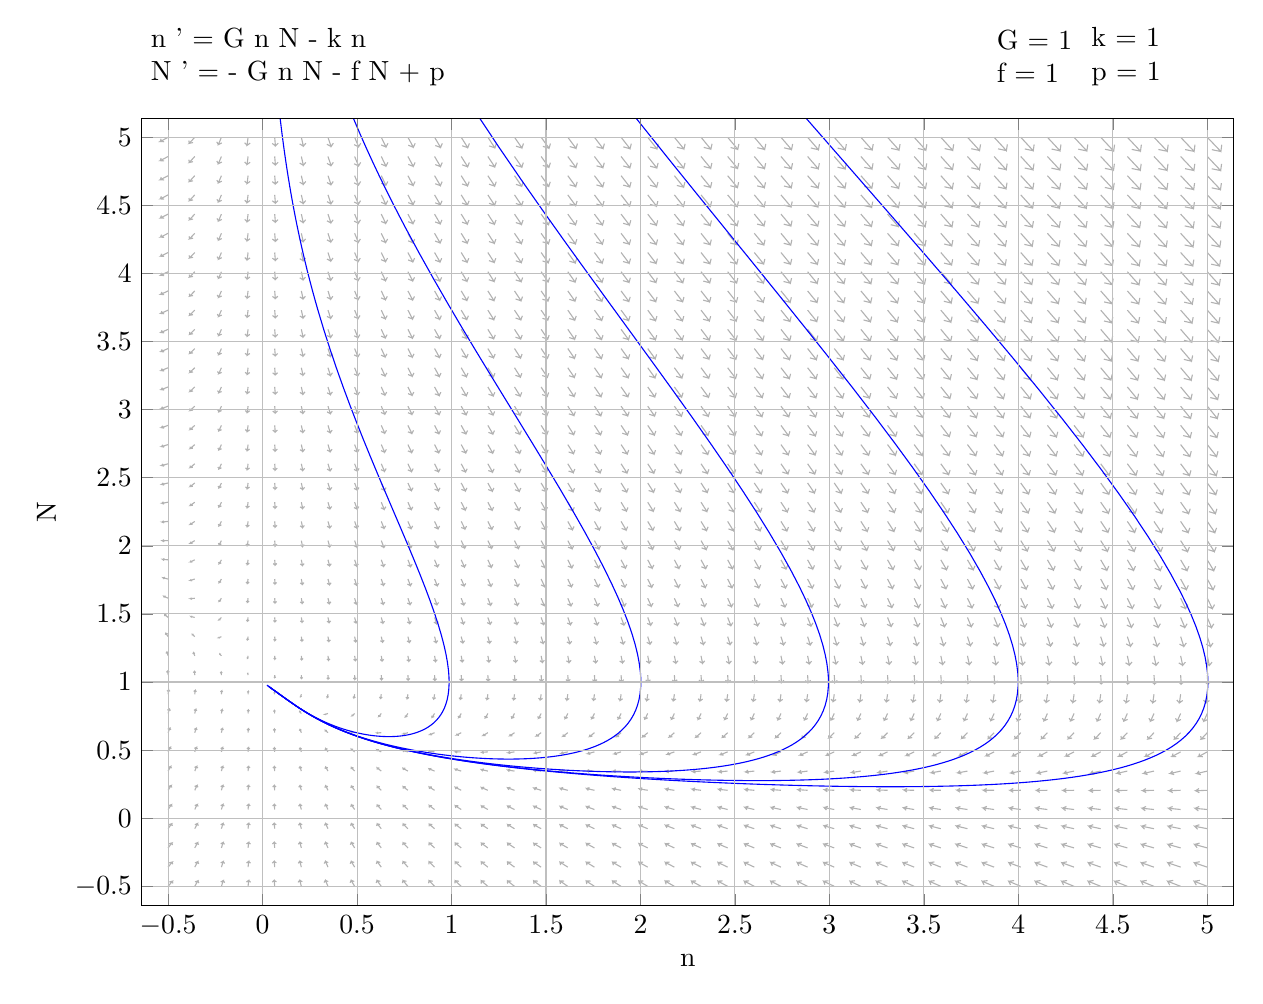
\begin{tikzpicture}

\begin{axis}[%
width=5.4625in,
height=0.614583in,
at={(0.552083in,5.21875in)},
scale only axis,
every outer x axis line/.append style={black},
every x tick label/.append style={font=\color{black}},
xmin=0,
xmax=1,
xtick={-1},
xticklabels={\empty},
every outer y axis line/.append style={black},
every y tick label/.append style={font=\color{black}},
ymin=0,
ymax=1,
ytick={-1},
yticklabels={\empty},
hide axis,
axis x line*=bottom,
axis y line*=left
]
\node[right, align=left, inner sep=0mm, text=black]
at (axis cs:0.00806451612903225,0.495614035087719,0) {n ' = G n N - k n\\N ' = - G n N - f N + p};
\node[right, align=left, inner sep=0mm, text=black]
at (axis cs:0.869047619047619,0.5,0) {k = 1\\p = 1};
\node[right, align=left, inner sep=0mm, text=black]
at (axis cs:0.782380952380952,0.5,0) {G = 1\\f = 1};
\node[right, align=left, inner sep=0mm, text=black]
at (axis cs:0.7,0.5,0) { \\ };
\end{axis}

\begin{axis}[%
width=5.4625in,
height=3.9375in,
at={(0.552083in,1.28125in)},
scale only axis,
unbounded coords=jump,
separate axis lines,
every outer x axis line/.append style={black},
every x tick label/.append style={font=\color{black}},
xmin=-0.641025641025641,
xmax=5.14102564102564,
xlabel={n},
xmajorgrids,
every outer y axis line/.append style={black},
every y tick label/.append style={font=\color{black}},
ymin=-0.641025641025641,
ymax=5.14102564102564,
ylabel={N},
ymajorgrids,
every outer z axis line/.append style={black},
every z tick label/.append style={font=\color{black}},
zmin=-50,
zmax=50,
view={0}{90}
]
\addplot [color=white!70!black,solid,forget plot]
  table[row sep=crcr]{%
-0.5	-0.5\\
-0.47741325856428	-0.462355430940466\\
-0.493600423259879	-0.468002116299396\\
-0.47741325856428	-0.462355430940466\\
-0.474778138730112	-0.479295487017256\\
nan	0\\
-0.5	-0.358974358974359\\
-0.478580477021227	-0.321793300218753\\
-0.49430159860376	-0.327592737100742\\
-0.478580477021227	-0.321793300218753\\
-0.475711069225957	-0.338302498590128\\
nan	0\\
-0.5	-0.217948717948718\\
-0.47984373710355	-0.18124310235834\\
-0.495067019870079	-0.187215721311341\\
-0.47984373710355	-0.18124310235834\\
-0.47671421207489	-0.197293852759566\\
nan	0\\
-0.5	-0.0769230769230769\\
-0.481221179799735	-0.0407067808225658\\
-0.495908899884942	-0.0468769646026529\\
-0.481221179799735	-0.0407067808225658\\
-0.477800751834687	-0.0562663747027854\\
nan	0\\
-0.5	0.0641025641025641\\
-0.482736187458047	0.0998126421003031\\
-0.496842850720067	0.0934155718364697\\
-0.482736187458047	0.0998126421003031\\
-0.478987811721198	0.084783665565493\\
nan	0\\
-0.5	0.205128205128205\\
-0.484419374789796	0.240310262054473\\
-0.497889076584424	0.233650801279144\\
-0.484419374789796	0.240310262054473\\
-0.48029804812129	0.225860488674042\\
nan	0\\
-0.5	0.346153846153846\\
-0.486311457725772	0.380777806023952\\
-0.499074010375567	0.373812753631477\\
-0.486311457725772	0.380777806023952\\
-0.481762030440514	0.366968482494363\\
nan	0\\
-0.5	0.487179487179487\\
-0.488467347428049	0.521200812266744\\
-0.500432474471448	0.513877577883555\\
-0.488467347428049	0.521200812266744\\
-0.48342181192782	0.508111251597579\\
nan	0\\
-0.5	0.628205128205128\\
-0.490961747586587	0.661553162971859\\
-0.502010232002294	0.653808315645193\\
-0.490961747586587	0.661553162971859\\
-0.485336214618928	0.649289189438486\\
nan	0\\
-0.5	0.769230769230769\\
-0.493895827344398	0.801786356727313\\
-0.503865976015215	0.79354572364225\\
-0.493895827344398	0.801786356727313\\
-0.487588182266943	0.790493637314449\\
nan	0\\
-0.5	0.91025641025641\\
-0.497401571904985	0.941808751410161\\
-0.506069185621927	0.932992656087789\\
-0.497401571904985	0.941808751410161\\
-0.490293015045052	0.931693442040282\\
nan	0\\
-0.5	1.05128205128205\\
-0.501630623050966	1.08144857772491\\
-0.508683067746391	1.07199096402931\\
-0.501630623050966	1.08144857772491\\
-0.49359980452496	1.0728062755548\\
nan	0\\
-0.5	1.19230769230769\\
-0.506689888496183	1.22040522399166\\
-0.511707304868321	1.21030349236243\\
-0.506689888496183	1.22040522399166\\
-0.497658539026336	1.21364843661052\\
nan	0\\
-0.5	1.33333333333333\\
-0.512460578630736	1.35825449059481\\
-0.514952694356883	1.34766299875868\\
-0.512460578630736	1.35825449059481\\
-0.502492115726147	1.35389328807405\\
nan	0\\
-0.5	1.47435897435897\\
-0.51835011850026	1.49469288945386\\
-0.517928561723902	1.48400518530033\\
-0.51835011850026	1.49469288945386\\
-0.507761604176461	1.49318024455046\\
nan	0\\
-0.5	1.61538461538462\\
-0.523417875734299	1.63002078771855\\
-0.520051556097494	1.6197754670848\\
-0.523417875734299	1.63002078771855\\
-0.512733469930525	1.63148440495195\\
nan	0\\
-0.5	1.75641025641026\\
-0.527093804141437	1.76513537977784\\
-0.521146943740901	1.7557443917322\\
-0.527093804141437	1.76513537977784\\
-0.516784382057111	1.76929129380292\\
nan	0\\
-0.5	1.8974358974359\\
-0.529513760220849	1.90080889860399\\
-0.521502882446618	1.89241855819835\\
-0.529513760220849	1.90080889860399\\
-0.51981638186257	1.90717543830878\\
nan	0\\
-0.5	2.03846153846154\\
-0.53110524725551	2.03730949226689\\
-0.521485661530195	2.02987879431141\\
-0.53110524725551	2.03730949226689\\
-0.522061684627519	2.04543141793916\\
nan	0\\
-0.5	2.17948717948718\\
-0.53222198507941	2.17458383393162\\
-0.521329553166696	2.16799934132843\\
-0.53222198507941	2.17458383393162\\
-0.523781225944477	2.18411033386814\\
nan	0\\
-0.5	2.32051282051282\\
-0.533077258989841	2.31248435959296\\
-0.521146966062922	2.30662358312146\\
-0.533077258989841	2.31248435959296\\
-0.525161196522855	2.32316221261638\\
nan	0\\
-0.5	2.46153846153846\\
-0.533786583466576	2.45086901412796\\
-0.520983246573979	2.44562320248447\\
-0.533786583466576	2.45086901412796\\
-0.526317970279228	2.46251649421776\\
nan	0\\
-0.5	2.6025641025641\\
-0.534411018026092	2.58962555978629\\
-0.520853076923812	2.58490436811311\\
-0.534411018026092	2.58962555978629\\
-0.527322348312717	2.60210987712616\\
nan	0\\
-0.5	2.74358974358974\\
-0.534983180003229	2.72867044623543\\
-0.520758401663681	2.72440044044091\\
-0.534983180003229	2.72867044623543\\
-0.52821805034084	2.74189203044253\\
nan	0\\
-0.5	2.88461538461538\\
-0.535520934840264	2.86794229275159\\
-0.520696381422236	2.86406398660066\\
-0.535520934840264	2.86794229275159\\
-0.529032927354134	2.88182445402079\\
nan	0\\
-0.5	3.02564102564103\\
-0.536034378342134	3.00739577078425\\
-0.5206627511253	3.00386075265575\\
-0.536034378342134	3.00739577078425\\
-0.529785378553688	3.02187794182682\\
nan	0\\
-0.5	3.16666666666667\\
-0.536529416414568	3.14699698090498\\
-0.520653170049775	3.14376553252984\\
-0.536529416414568	3.14699698090498\\
-0.53048801293062	3.16203024073713\\
nan	0\\
-0.5	3.30769230769231\\
-0.537009636153727	3.28672018053853\\
-0.520663713519164	3.28375940964623\\
-0.537009636153727	3.28672018053853\\
-0.531149777096054	3.30226422772309\\
nan	0\\
-0.5	3.44871794871795\\
-0.537477307706865	3.42654551012698\\
-0.520691005747062	3.42382791477755\\
-0.537477307706865	3.42654551012698\\
-0.531777225042548	3.44256656863098\\
nan	0\\
-0.5	3.58974358974359\\
-0.537933934213731	3.56645741230546\\
-0.520732209590079	3.56395978198346\\
-0.537933934213731	3.56645741230546\\
-0.532375298309145	3.58292674909033\\
nan	0\\
-0.5	3.73076923076923\\
-0.538380560973622	3.70644352310989\\
-0.520784965766701	3.70414609516429\\
-0.538380560973622	3.70644352310989\\
-0.53294781959637	3.7233363756511\\
nan	0\\
-0.5	3.87179487179487\\
-0.53881795315921	3.84649388446789\\
-0.520847320379701	3.84437969237618\\
-0.53881795315921	3.84649388446789\\
-0.533497814043194	3.86378866895578\\
nan	0\\
-0.5	4.01282051282051\\
-0.539246700079255	3.98660037702288\\
-0.520917656106071	3.98465474274236\\
-0.539246700079255	3.98660037702288\\
-0.534027724004886	4.00427809278199\\
nan	0\\
-0.5	4.15384615384615\\
-0.539667277511346	4.12675630578963\\
-0.52099463224381	4.12496644082875\\
-0.539667277511346	4.12675630578963\\
-0.534539556272074	4.14480007958442\\
nan	0\\
-0.5	4.29487179487179\\
-0.540080085627603	4.26695609320899\\
-0.521077134523621	4.26531078230093\\
-0.540080085627603	4.26695609320899\\
-0.535034985355024	4.28535082511473\\
nan	0\\
-0.5	4.43589743589744\\
-0.540485472461071	4.40719504870489\\
-0.521164233924612	4.40568439674738\\
-0.540485472461071	4.40719504870489\\
-0.535515427520887	4.42592713297792\\
nan	0\\
-0.5	4.57692307692308\\
-0.540883748669413	4.54746919347307\\
-0.521255153206088	4.54608442134072\\
-0.540883748669413	4.54746919347307\\
-0.535982094931091	4.56652629567543\\
nan	0\\
-0.5	4.71794871794872\\
-0.541275196985568	4.68777512566961\\
-0.521349239820121	4.68650840410695\\
-0.541275196985568	4.68777512566961\\
-0.536436035959674	4.70714600259974\\
nan	0\\
-0.5	4.85897435897436\\
-0.541660078382675	4.82810991552141\\
-0.521445944004636	4.82695422896163\\
-0.541660078382675	4.82810991552141\\
-0.536878165731109	4.84778426815297\\
nan	0\\
-0.5	5\\
-0.542038636182895	4.96847102286283\\
-0.521544801043734	4.96742005695826\\
-0.542038636182895	4.96847102286283\\
-0.537309289612319	4.9884393750497\\
nan	0\\
-0.358974358974359	-0.5\\
-0.342519100308186	-0.459645437080576\\
-0.357544318637894	-0.46763799128986\\
-0.342519100308186	-0.459645437080576\\
-0.337367037178182	-0.475865620622946\\
nan	0\\
-0.358974358974359	-0.358974358974359\\
-0.343304032104451	-0.319460637177059\\
-0.357883560614749	-0.327397171998772\\
-0.343304032104451	-0.319460637177059\\
-0.338126699716099	-0.335232335433726\\
nan	0\\
-0.358974358974359	-0.217948717948718\\
-0.344153738330218	-0.179314814359819\\
-0.358258400420685	-0.187199830275453\\
-0.344153738330218	-0.179314814359819\\
-0.338941448626236	-0.194610140597524\\
nan	0\\
-0.358974358974359	-0.0769230769230769\\
-0.345081272461228	-0.0392132706731508\\
-0.358676649977649	-0.0470529409198459\\
-0.345081272461228	-0.0392132706731508\\
-0.339821746852686	-0.0539994841764113\\
nan	0\\
-0.358974358974359	0.0641025641025641\\
-0.346103993604765	0.100837256649634\\
-0.359148776352411	0.0930344402279114\\
-0.346103993604765	0.100837256649634\\
-0.340781430078876	0.0865992575431145\\
nan	0\\
-0.358974358974359	0.205128205128205\\
-0.347245612295426	0.240827915641733\\
-0.359689163927488	0.233050189157408\\
-0.347245612295426	0.240827915641733\\
-0.341839308670724	0.227185815817941\\
nan	0\\
-0.358974358974359	0.346153846153846\\
-0.348539550039079	0.38074655308635\\
-0.360318169452789	0.372977443240419\\
-0.348539550039079	0.38074655308635\\
-0.343021815986537	0.367760038772779\\
nan	0\\
-0.358974358974359	0.487179487179487\\
-0.350034705958455	0.520575476660329\\
-0.361065599233437	0.512791593070053\\
-0.350034705958455	0.520575476660329\\
-0.344367604493016	0.5083217665621\\
nan	0\\
-0.358974358974359	0.628205128205128\\
-0.351805855519915	0.660286829625634\\
-0.361976831911374	0.652454445063093\\
-0.351805855519915	0.660286829625634\\
-0.345935981201121	0.648870193335871\\
nan	0\\
-0.358974358974359	0.769230769230769\\
-0.35397338862406	0.799831944945694\\
-0.363123973657881	0.791901834818792\\
-0.35397338862406	0.799831944945694\\
-0.347823385800418	0.789401349643642\\
nan	0\\
-0.358974358974359	0.91025641025641\\
-0.356742310013594	0.93911361467773\\
-0.364626225807153	0.931014465591526\\
-0.356742310013594	0.93911361467773\\
-0.350197623596493	0.929898441111143\\
nan	0\\
-0.358974358974359	1.05128205128205\\
-0.360477195943091	1.07790373472816\\
-0.366681765713999	1.06954152045215\\
-0.360477195943091	1.07790373472816\\
-0.353370923990944	1.07029293893651\\
nan	0\\
-0.358974358974359	1.19230769230769\\
-0.365789650357942	1.21557704431735\\
-0.369562400945282	1.20689241586856\\
-0.365789650357942	1.21557704431735\\
-0.357927724940452	1.21030006156035\\
nan	0\\
-0.358974358974359	1.33333333333333\\
-0.373080150594776	1.3504617945867\\
-0.373130528421992	1.34179680830558\\
-0.373080150594776	1.3504617945867\\
-0.36456629779531	1.34884970411579\\
nan	0\\
-0.358974358974359	1.47435897435897\\
-0.37973881763296	1.48105330755586\\
-0.375183063334601	1.47385389293214\\
-0.37973881763296	1.48105330755586\\
-0.371835896736158	1.48423612226144\\
nan	0\\
-0.358974358974359	1.61538461538462\\
-0.382181607180201	1.61165487906582\\
-0.374286998638749	1.60697198791\\
-0.382181607180201	1.61165487906582\\
-0.376151866798147	1.61857561201292\\
nan	0\\
-0.358974358974359	1.75641025641026\\
-0.382470337734511	1.74551563187619\\
-0.372697887972949	1.74291002454637\\
-0.382470337734511	1.74551563187619\\
-0.378145200239981	1.75465801392645\\
nan	0\\
-0.358974358974359	1.8974358974359\\
-0.382420071674796	1.88169377605132\\
-0.37145082751852	1.88055498429158\\
-0.382420071674796	1.88169377605132\\
-0.379321888210809	1.8922778406418\\
nan	0\\
-0.358974358974359	2.03846153846154\\
-0.382428839451426	2.01916433362459\\
-0.370568194099068	2.01908987495641\\
-0.382428839451426	2.01916433362459\\
-0.380216796517544	2.03081711519494\\
nan	0\\
-0.358974358974359	2.17948717948718\\
-0.382532430044687	2.15739234264482\\
-0.369941299512999	2.15813127592995\\
-0.382532430044687	2.15739234264482\\
-0.380988717934178	2.16991031146511\\
nan	0\\
-0.358974358974359	2.32051282051282\\
-0.382709316741962	2.29610301304447\\
-0.369486377544595	2.29749221584308\\
-0.382709316741962	2.29610301304447\\
-0.381691281278768	2.30935969472688\\
nan	0\\
-0.358974358974359	2.46153846153846\\
-0.382936322562438	2.43514426856362\\
-0.369149185242304	2.43707203555905\\
-0.382936322562438	2.43514426856362\\
-0.382346281729724	2.44905301735309\\
nan	0\\
-0.358974358974359	2.6025641025641\\
-0.383196256216588	2.5744251785107\\
-0.368894956030569	2.57681138141617\\
-0.383196256216588	2.5744251785107\\
-0.382964418057269	2.58892233003728\\
nan	0\\
-0.358974358974359	2.74358974358974\\
-0.38347727947324	2.71388767399341\\
-0.368700885924492	2.71667256474759\\
-0.38347727947324	2.71388767399341\\
-0.383551920722659	2.72892402499703\\
nan	0\\
-0.358974358974359	2.88461538461538\\
-0.383771358469904	2.8534926199424\\
-0.368551567452995	2.85663019947041\\
-0.383771358469904	2.8534926199424\\
-0.384112949789485	2.86902869921818\\
nan	0\\
-0.358974358974359	3.02564102564103\\
-0.384073026994315	2.99321245728613\\
-0.368436284499604	2.99666636078761\\
-0.384073026994315	2.99321245728613\\
-0.384650568677052	3.00921569479759\\
nan	0\\
-0.358974358974359	3.16666666666667\\
-0.384378538976109	3.13302706567534\\
-0.368347384727752	3.1367679009723\\
-0.384378538976109	3.13302706567534\\
-0.385167185223417	3.14946999097317\\
nan	0\\
-0.358974358974359	3.30769230769231\\
-0.384685308825017	3.27292130884666\\
-0.368279274158407	3.27692487103769\\
-0.384685308825017	3.27292130884666\\
-0.385664773581233	3.28978034596302\\
nan	0\\
-0.358974358974359	3.44871794871795\\
-0.384991543134934	3.41288350995078\\
-0.36822777819497	3.41712954554079\\
-0.384991543134934	3.41288350995078\\
-0.386144997578553	3.43013813762108\\
nan	0\\
-0.358974358974359	3.58974358974359\\
-0.385295996246869	3.55290446657365\\
-0.368189724272631	3.5573757942065\\
-0.385295996246869	3.55290446657365\\
-0.386609285857602	3.57053661284276\\
nan	0\\
-0.358974358974359	3.73076923076923\\
-0.385597805914266	3.69297679250745\\
-0.368162662266849	3.69765866225101\\
-0.385597805914266	3.69297679250745\\
-0.387058881397738	3.71097038572096\\
nan	0\\
-0.358974358974359	3.87179487179487\\
-0.385896381251242	3.83309446477185\\
-0.368144672812422	3.83797408130954\\
-0.385896381251242	3.83309446477185\\
-0.387494876323931	3.85143509244798\\
nan	0\\
-0.358974358974359	4.01282051282051\\
-0.38619132525564	3.97325250378605\\
-0.368134233112641	3.97831866492607\\
-0.38619132525564	3.97325250378605\\
-0.387918237629871	3.99192714806671\\
nan	0\\
-0.358974358974359	4.15384615384615\\
-0.386482380526784	4.11344674240244\\
-0.368130121200127	4.11868956044744\\
-0.386482380526784	4.11344674240244\\
-0.388329826921986	4.13244357122366\\
nan	0\\
-0.358974358974359	4.29487179487179\\
-0.386769390768791	4.25367365575014\\
-0.368131346450048	4.25908433953803\\
-0.386769390768791	4.25367365575014\\
-0.388730416010874	4.27298185543525\\
nan	0\\
-0.358974358974359	4.43589743589744\\
-0.387052273186627	4.39393023363134\\
-0.368137098356422	4.3995009157581\\
-0.387052273186627	4.39393023363134\\
-0.389120699489471	4.41353987286424\\
nan	0\\
-0.358974358974359	4.57692307692308\\
-0.387330998497141	4.53421388329468\\
-0.368146708233207	4.5399374815025\\
-0.387330998497141	4.53421388329468\\
-0.389501305047406	4.55411580126389\\
nan	0\\
-0.358974358974359	4.71794871794872\\
-0.387605576328458	4.67452235428701\\
-0.368159620206801	4.680392459047\\
-0.387605576328458	4.67452235428701\\
-0.389872802037656	4.69470806772405\\
nan	0\\
-0.358974358974359	4.85897435897436\\
-0.387876044474972	4.81485367961379\\
-0.368175368984646	4.82086446204681\\
-0.387876044474972	4.81485367961379\\
-0.390235708664931	4.83531530479711\\
nan	0\\
-0.358974358974359	5\\
-0.388142460939523	4.95520612912493\\
-0.368193562631205	4.96135226489616\\
-0.388142460939523	4.95520612912493\\
-0.390590498068742	4.97593631587874\\
nan	0\\
-0.217948717948718	-0.5\\
-0.207971312840272	-0.457547119440535\\
-0.221577754512672	-0.467788632331263\\
-0.207971312840272	-0.457547119440535\\
-0.20035131423294	-0.472777334885486\\
nan	0\\
-0.217948717948718	-0.358974358974359\\
-0.208392296912818	-0.31765158832412\\
-0.221589915886148	-0.327659314260217\\
-0.208392296912818	-0.31765158832412\\
-0.200928530561029	-0.332437524778167\\
nan	0\\
-0.217948717948718	-0.217948717948718\\
-0.208848190817872	-0.177821873553207\\
-0.221610060056004	-0.187584795089149\\
-0.208848190817872	-0.177821873553207\\
-0.201546637858248	-0.192135058654571\\
nan	0\\
-0.217948717948718	-0.0769230769230769\\
-0.209346510060823	-0.0380685665050631\\
-0.221640800031695	-0.0475743676584934\\
-0.209346510060823	-0.0380685665050631\\
-0.202213544822688	-0.051875471602441\\
nan	0\\
-0.217948717948718	0.0641025641025641\\
-0.209897545518434	0.101594687772679\\
-0.221685928165048	0.0923598437792152\\
-0.209897545518434	0.101594687772679\\
-0.20293986632999	0.0883342575640732\\
nan	0\\
-0.217948717948718	0.205128205128205\\
-0.210515911816959	0.241149812074151\\
-0.221751155392973	0.232201531523307\\
-0.210515911816959	0.241149812074151\\
-0.20374035192	0.228485128457427\\
nan	0\\
-0.217948717948718	0.346153846153846\\
-0.211223332212663	0.38057199668542\\
-0.221845485566373	0.371927897959962\\
-0.211223332212663	0.38057199668542\\
-0.204636410300586	0.368565205091934\\
nan	0\\
-0.217948717948718	0.487179487179487\\
-0.212054043767027	0.519825579779852\\
-0.221983969171625	0.511505420545165\\
-0.212054043767027	0.519825579779852\\
-0.205660922871443	0.50855808345432\\
nan	0\\
-0.217948717948718	0.628205128205128\\
-0.21306637728898	0.658855928087258\\
-0.222193779457434	0.650881273287554\\
-0.21306637728898	0.658855928087258\\
-0.206868379516369	0.648440102957685\\
nan	0\\
-0.217948717948718	0.769230769230769\\
-0.214371106802684	0.797571061446413\\
-0.222529463200405	0.789963376568228\\
-0.214371106802684	0.797571061446413\\
-0.208359317092583	0.788174570995211\\
nan	0\\
-0.217948717948718	0.91025641025641\\
-0.216215410222723	0.935789926589767\\
-0.223118781623861	0.928563198621259\\
-0.216215410222723	0.935789926589767\\
-0.210352023457182	0.927696544758261\\
nan	0\\
-0.217948717948718	1.05128205128205\\
-0.21931529979849	1.07302678012696\\
-0.224341507454786	1.06616171601105\\
-0.21931529979849	1.07302678012696\\
-0.213469143032331	1.06684500693593\\
nan	0\\
-0.217948717948718	1.19230769230769\\
-0.226725807557914	1.20645429556016\\
-0.227629331488273	1.20001604218212\\
-0.226725807557914	1.20645429556016\\
-0.220556029862038	1.20440458698672\\
nan	0\\
-0.217948717948718	1.33333333333333\\
-0.232580786600388	1.32472623412647\\
-0.226039391203171	1.32365034672561\\
-0.232580786600388	1.32472623412647\\
-0.230342940806603	1.33096638105145\\
nan	0\\
-0.217948717948718	1.47435897435897\\
-0.230292085104026	1.45608922106551\\
-0.222021636634066	1.45848430526472\\
-0.230292085104026	1.45608922106551\\
-0.231156513280801	1.46465598884237\\
nan	0\\
-0.217948717948718	1.61538461538462\\
-0.229653687529216	1.59240500598761\\
-0.220397294305815	1.59637264641159\\
-0.229653687529216	1.59240500598761\\
-0.231887099004318	1.60222513120184\\
nan	0\\
-0.217948717948718	1.75641025641026\\
-0.229545261645738	1.73013015289747\\
-0.219496272658435	1.73511504802705\\
-0.229545261645738	1.73013015289747\\
-0.232636324414829	1.74091331987556\\
nan	0\\
-0.217948717948718	1.8974358974359\\
-0.229631040971957	1.86853441930109\\
-0.218900974531284	1.87428428198573\\
-0.229631040971957	1.86853441930109\\
-0.233351713598686	1.88012544349735\\
nan	0\\
-0.217948717948718	2.03846153846154\\
-0.229799950194796	2.00734882635582\\
-0.218466402494543	2.01371983192602\\
-0.229799950194796	2.00734882635582\\
-0.234022758547402	2.01964544804906\\
nan	0\\
-0.217948717948718	2.17948717948718\\
-0.230007051694772	2.14644241066647\\
-0.218128359365779	2.15334125787617\\
-0.230007051694772	2.14644241066647\\
-0.234650743776132	2.1593704247492\\
nan	0\\
-0.217948717948718	2.32051282051282\\
-0.230231600169577	2.28574054914286\\
-0.21785366766083	2.29310150999863\\
-0.230231600169577	2.28574054914286\\
-0.235239803345809	2.29924295110906\\
nan	0\\
-0.217948717948718	2.46153846153846\\
-0.230463155925092	2.42519622369995\\
-0.217623265072552	2.43297028555741\\
-0.230463155925092	2.42519622369995\\
-0.235794383991807	2.4392275045456\\
nan	0\\
-0.217948717948718	2.6025641025641\\
-0.230696165908253	2.56477766741252\\
-0.217425322732497	2.57292673596811\\
-0.230696165908253	2.56477766741252\\
-0.236318540308288	2.57930045994788\\
nan	0\\
-0.217948717948718	2.74358974358974\\
-0.230927581464551	2.70446228740231\\
-0.217252058362942	2.71295580837958\\
-0.230927581464551	2.70446228740231\\
-0.236815786456661	2.7194452401375\\
nan	0\\
-0.217948717948718	2.88461538461538\\
-0.231155713401891	2.84423337090682\\
-0.217098111338799	2.8530462261561\\
-0.231155713401891	2.84423337090682\\
-0.237289118193079	2.85964972388269\\
nan	0\\
-0.217948717948718	3.02564102564103\\
-0.231379642630545	2.98407816415355\\
-0.216959649854129	2.99318929142934\\
-0.231379642630545	2.98407816415355\\
-0.237741080597865	2.99990475377025\\
nan	0\\
-0.217948717948718	3.16666666666667\\
-0.231598899985046	3.12398668572955\\
-0.216833850139869	3.1333781345016\\
-0.231598899985046	3.12398668572955\\
-0.238173840608427	3.14020322551977\\
nan	0\\
-0.217948717948718	3.30769230769231\\
-0.231813284660589	3.2639509589876\\
-0.216718577470851	3.27360722192105\\
-0.231813284660589	3.2639509589876\\
-0.238589251823204	3.28053950527698\\
nan	0\\
-0.217948717948718	3.44871794871795\\
-0.232022757662824	3.40396449628551\\
-0.216612182640481	3.41387202208671\\
-0.232022757662824	3.40396449628551\\
-0.238988908856703	3.42090904194377\\
nan	0\\
-0.217948717948718	3.58974358974359\\
-0.232227377551363	3.54402194123145\\
-0.216513367542535	3.55416877088443\\
-0.232227377551363	3.54402194123145\\
-0.239374191798604	3.56130810068575\\
nan	0\\
-0.217948717948718	3.73076923076923\\
-0.232427260857527	3.68411881372502\\
-0.216421093723832	3.69449430311108\\
-0.232427260857527	3.68411881372502\\
-0.239746302245936	3.70173357456549\\
nan	0\\
-0.217948717948718	3.87179487179487\\
-0.232622557314291	3.82425132397648\\
-0.216334518550021	3.8348459284806\\
-0.232622557314291	3.82425132397648\\
-0.240106292459217	3.84218284816339\\
nan	0\\
-0.217948717948718	4.01282051282051\\
-0.232813434193207	3.96441623406593\\
-0.216252949631215	3.97522133863118\\
-0.232813434193207	3.96441623406593\\
-0.240455089008507	3.98265369675343\\
nan	0\\
-0.217948717948718	4.15384615384615\\
-0.233000066352863	4.10461075304063\\
-0.216175811630238	4.11561853618125\\
-0.233000066352863	4.10461075304063\\
-0.240793512033001	4.12314421038332\\
nan	0\\
-0.217948717948718	4.29487179487179\\
-0.233182629928088	4.24483245616364\\
-0.216102621657238	4.25603577978124\\
-0.233182629928088	4.24483245616364\\
-0.241122291011317	4.26365273577093\\
nan	0\\
-0.217948717948718	4.43589743589744\\
-0.233361298370019	4.38507922187444\\
-0.216032970737879	4.39647154097601\\
-0.233361298370019	4.38507922187444\\
-0.241442077749379	4.40417783118666\\
nan	0\\
-0.217948717948718	4.57692307692308\\
-0.233536240018783	4.52534918195248\\
-0.215966509655115	4.53692446992615\\
-0.233536240018783	4.52534918195248\\
-0.241753457140411	4.54471823096118\\
nan	0\\
-0.217948717948718	4.71794871794872\\
-0.233707616681586	4.66564068166785\\
-0.21590293799151	4.6773933678689\\
-0.233707616681586	4.66564068166785\\
-0.242056956131942	4.68527281723533\\
nan	0\\
-0.217948717948718	4.85897435897436\\
-0.233875582872	4.8059522475872\\
-0.215841995548225	4.81787716477252\\
-0.233875582872	4.8059522475872\\
-0.242353051241806	4.82584059723417\\
nan	0\\
-0.217948717948718	5\\
-0.234040285483192	4.94628256131874\\
-0.215783455552535	4.9583749010395\\
-0.234040285483192	4.94628256131874\\
-0.242642174893164	4.96642068480674\\
nan	0\\
-0.0769230769230769	-0.5\\
-0.0734613971088257	-0.456152055686151\\
-0.0854618871315633	-0.468441019026743\\
-0.0734613971088257	-0.456152055686151\\
-0.0635379149746389	-0.470171858933869\\
nan	0\\
-0.0769230769230769	-0.358974358974359\\
-0.073585538776434	-0.316467976918058\\
-0.0852133957345021	-0.328385506998288\\
-0.073585538776434	-0.316467976918058\\
-0.0639602047063517	-0.330054276071609\\
nan	0\\
-0.0769230769230769	-0.217948717948718\\
-0.0737194147305438	-0.176874396364451\\
-0.0849490937843705	-0.188395777291598\\
-0.0737194147305438	-0.176874396364451\\
-0.0644119329922369	-0.189997608387864\\
nan	0\\
-0.0769230769230769	-0.0769230769230769\\
-0.073865139890078	-0.0373883195678771\\
-0.0846662103387777	-0.0484842625161873\\
-0.073865139890078	-0.0373883195678771\\
-0.0648988316611778	-0.0500132310326868\\
nan	0\\
-0.0769230769230769	0.0641025641025641\\
-0.0740256571619847	0.101967474405058\\
-0.0843611106659357	0.0913323562545826\\
-0.0740256571619847	0.101967474405058\\
-0.065428655514689	0.0898836463740364\\
nan	0\\
-0.0769230769230769	0.205128205128205\\
-0.0742052494734534	0.24116133679902\\
-0.0840288806260443	0.231030854160182\\
-0.0742052494734534	0.24116133679902\\
-0.0660123147906366	0.22967194043537\\
nan	0\\
-0.0769230769230769	0.346153846153846\\
-0.0744105269529802	0.380147169278684\\
-0.0836626227252187	0.370577309833757\\
-0.0744105269529802	0.380147169278684\\
-0.0666659611627997	0.369321034848708\\
nan	0\\
-0.0769230769230769	0.487179487179487\\
-0.0746525438096462	0.518853424111846\\
-0.083252187976765	0.509918876310496\\
-0.0746525438096462	0.518853424111846\\
-0.0674152195105859	0.50878360975378\\
nan	0\\
-0.0769230769230769	0.628205128205128\\
-0.074952069533262	0.657158547103789\\
-0.0827817264748717	0.648965273281645\\
-0.074952069533262	0.657158547103789\\
-0.0683050170255412	0.647979769586737\\
nan	0\\
-0.0769230769230769	0.769230769230769\\
-0.0753560902581004	0.794824884758719\\
-0.0822247151395808	0.787538396766578\\
-0.0753560902581004	0.794824884758719\\
-0.0694276573756059	0.78675490343409\\
nan	0\\
-0.0769230769230769	0.91025641025641\\
-0.0760158471320466	0.931252299705969\\
-0.0815369884317455	0.925180340318859\\
-0.0760158471320466	0.931252299705969\\
-0.0710390437069659	0.924726725423344\\
nan	0\\
-0.0769230769230769	1.05128205128205\\
-0.0785103834794031	1.0631868504545\\
-0.0810103913056167	1.05921858406368\\
-0.0785103834794031	1.0631868504545\\
-0.0750579917193937	1.06001223734185\\
nan	0\\
-0.0769230769230769	1.19230769230769\\
-0.0795522939332646	1.17442901663842\\
-0.0742938599128893	1.17913531508665\\
-0.0795522939332646	1.17442901663842\\
-0.0832331977475273	1.18044992359175\\
nan	0\\
-0.0769230769230769	1.33333333333333\\
-0.0795510392907683	1.30968167202411\\
-0.0728497352531553	1.31612017982495\\
-0.0795510392907683	1.30968167202411\\
-0.0846755659077664	1.3174341610088\\
nan	0\\
-0.0769230769230769	1.47435897435897\\
-0.0797004977563991	1.44688502773746\\
-0.0719987848510247	1.45443285651559\\
-0.0797004977563991	1.44688502773746\\
-0.0857357581617801	1.45582156693225\\
nan	0\\
-0.0769230769230769	1.61538461538462\\
-0.0798583531057507	1.58493112498937\\
-0.0713643976521384	1.59333335306228\\
-0.0798583531057507	1.58493112498937\\
-0.0865911428497588	1.59480099115362\\
nan	0\\
-0.0769230769230769	1.75641025641026\\
-0.0800081124403116	1.7234683517347\\
-0.0708471256162519	1.73257966425806\\
-0.0800081124403116	1.7234683517347\\
-0.0873180779540305	1.73412218201668\\
nan	0\\
-0.0769230769230769	1.8974358974359\\
-0.0801476892135667	1.86233368935942\\
-0.0704047535073012	1.87205819870974\\
-0.0801476892135667	1.86233368935942\\
-0.0879558575455383	1.87367050485499\\
nan	0\\
-0.0769230769230769	2.03846153846154\\
-0.0802776900865569	2.00143654873128\\
-0.0700150587049478	2.01170539235949\\
-0.0802776900865569	2.00143654873128\\
-0.088527553570078	2.01338269894123\\
nan	0\\
-0.0769230769230769	2.17948717948718\\
-0.0803992087825427	2.14072075244575\\
-0.0696647624643447	2.15148164759331\\
-0.0803992087825427	2.14072075244575\\
-0.0890479759850612	2.15321971352304\\
nan	0\\
-0.0769230769230769	2.32051282051282\\
-0.0805133159669199	2.2801487737869\\
-0.069345232572286	2.29136042804371\\
-0.0805133159669199	2.2801487737869\\
-0.089527255935248	2.29315554756563\\
nan	0\\
-0.0769230769230769	2.46153846153846\\
-0.0806209459096795	2.4196941545848\\
-0.0690505084752836	2.43132297942425\\
-0.0806209459096795	2.4196941545848\\
-0.0899726619521138	2.43317191391755\\
nan	0\\
-0.0769230769230769	2.6025641025641\\
-0.0807228873935976	2.55933745865146\\
-0.0687762832742807	2.57135549920762\\
-0.0807228873935976	2.55933745865146\\
-0.090389605230602	2.57325540444288\\
nan	0\\
-0.0769230769230769	2.74358974358974\\
-0.0808198011343381	2.6990639389993\\
-0.0685193327233497	2.71144749932362\\
-0.0808198011343381	2.6990639389993\\
-0.0907822350185697	2.71339586142925\\
nan	0\\
-0.0769230769230769	2.88461538461538\\
-0.0809122414200623	2.83886211018057\\
-0.0682771734622638	2.85159080138677\\
-0.0809122414200623	2.83886211018057\\
-0.0911538106796695	2.85358538363526\\
nan	0\\
-0.0769230769230769	3.02564102564103\\
-0.0810006757303271	2.97872283177026\\
-0.0680478476204608	2.99177889022968\\
-0.0810006757303271	2.97872283177026\\
-0.0915069445558434	2.9938176896333\\
nan	0\\
-0.0769230769230769	3.16666666666667\\
-0.0810855010054632	3.11863869648529\\
-0.0678297812354022	3.1320064815191\\
-0.0810855010054632	3.11863869648529\\
-0.0918437663260924	3.1340876935603\\
nan	0\\
-0.0769230769230769	3.30769230769231\\
-0.0811670567147782	3.25860360810163\\
-0.0676216878795984	3.27226922303091\\
-0.0811670567147782	3.25860360810163\\
-0.0921660376749372	3.27439121292676\\
nan	0\\
-0.0769230769230769	3.44871794871795\\
-0.0812456352441685	3.39861248210592\\
-0.0674225010948348	3.41256348250926\\
-0.0812456352441685	3.39861248210592\\
-0.0924752344008472	3.4147247616698\\
nan	0\\
-0.0769230769230769	3.58974358974359\\
-0.0813214901445636	3.53866102827028\\
-0.0672313258097911	3.5528861934069\\
-0.0813214901445636	3.53866102827028\\
-0.0927726065464442	3.55508540001765\\
nan	0\\
-0.0769230769230769	3.73076923076923\\
-0.0813948427044952	3.67874558942484\\
-0.067047402633973	3.69323474038281\\
-0.0813948427044952	3.67874558942484\\
-0.0930592233061664	3.69547062327351\\
nan	0\\
-0.0769230769230769	3.87179487179487\\
-0.0814658872169272	3.81886301971028\\
-0.0668700811076234	3.83360687276219\\
-0.0814658872169272	3.81886301971028\\
-0.0933360071499208	3.83587827790912\\
nan	0\\
-0.0769230769230769	4.01282051282051\\
-0.0815347952278994	3.95901059115318\\
-0.0666987993196194	3.97400063807717\\
-0.0815347952278994	3.95901059115318\\
-0.0936037601532859	3.97630649722959\\
nan	0\\
-0.0769230769230769	4.15384615384615\\
-0.0816017189879944	4.09918592094139\\
-0.0665330681423272	4.11441433029659\\
-0.0816017189879944	4.09918592094139\\
-0.0938631845947111	4.11675365132905\\
nan	0\\
-0.0769230769230769	4.29487179487179\\
-0.0816667942761073	4.2393869140811\\
-0.0663724588725237	4.25484644898005\\
-0.0816667942761073	4.2393869140811\\
-0.0941148992678727	4.25721830765656\\
nan	0\\
-0.0769230769230769	4.43589743589744\\
-0.0817301427257435	4.37961171765577\\
-0.0662165934245259	4.3952956666776\\
-0.0817301427257435	4.37961171765577\\
-0.0943594525453612	4.39769919957893\\
nan	0\\
-0.0769230769230769	4.57692307692308\\
-0.0817918737543558	4.51985868395432\\
-0.066065136462784	4.53576080263713\\
-0.0817918737543558	4.51985868395432\\
-0.0945973329471603	4.53819520105277\\
nan	0\\
-0.0769230769230769	4.71794871794872\\
-0.081852086173738	4.66012634046338\\
-0.0659177890272043	4.67624080139631\\
-0.081852086173738	4.66012634046338\\
-0.0948289777698751	4.67870530602164\\
nan	0\\
-0.0769230769230769	4.85897435897436\\
-0.0819108695424166	4.80041336523102\\
-0.0657742833207789	4.81673471519918\\
-0.0819108695424166	4.80041336523102\\
-0.0950547801924504	4.81922861150885\\
nan	0\\
-0.0769230769230769	5\\
-0.08196830530796	4.94071856647762\\
-0.0656343784119012	4.95724168943812\\
-0.08196830530796	4.94071856647762\\
-0.0952750951730889	4.95976430363056\\
nan	0\\
0.0641025641025641	-0.5\\
0.0613049102589753	-0.455424048758818\\
0.0510002186017565	-0.46949624759207\\
0.0613049102589753	-0.455424048758818\\
0.0732881942223473	-0.468097420670276\\
nan	0\\
0.0641025641025641	-0.358974358974359\\
0.0613876533767019	-0.315904605421435\\
0.0514346882062296	-0.329504259168778\\
0.0613876533767019	-0.315904605421435\\
0.0729695649826915	-0.328146803805847\\
nan	0\\
0.0641025641025641	-0.217948717948718\\
0.0614756383395834	-0.176498594593895\\
0.051901185229772	-0.189590363041087\\
0.0614756383395834	-0.176498594593895\\
0.0726262469071832	-0.188276900159597\\
nan	0\\
0.0641025641025641	-0.0769230769230769\\
0.061569742043645	-0.0372301369425869\\
0.0524063536661982	-0.0497712244514637\\
0.061569742043645	-0.0372301369425869\\
0.0722528236564432	-0.0485048134220041\\
nan	0\\
0.0641025641025641	0.0641025641025641\\
0.061671077338187	0.101867217437506\\
0.0529593600337648	0.0899299497459289\\
0.061671077338187	0.101867217437506\\
0.0718416867012355	0.0911456931281175\\
nan	0\\
0.0641025641025641	0.205128205128205\\
0.0617810626838032	0.24074453012055\\
0.0535734318613453	0.229479257268156\\
0.0617810626838032	0.24074453012055\\
0.0713815943575176	0.230640007977536\\
nan	0\\
0.0641025641025641	0.346153846153846\\
0.0619014655060741	0.37932569676683\\
0.0542688324317751	0.368823866933812\\
0.0619014655060741	0.37932569676683\\
0.0708547577382671	0.369924416232057\\
nan	0\\
0.0641025641025641	0.487179487179487\\
0.062034197423716	0.517481059024611\\
0.0550793144660894	0.507873495801362\\
0.062034197423716	0.517481059024611\\
0.0702301003886515	0.508907679140786\\
nan	0\\
0.0641025641025641	0.628205128205128\\
0.0621794720386779	0.65495600194898\\
0.0560686812218809	0.646449966809853\\
0.0621794720386779	0.65495600194898\\
0.0694441180938067	0.647411512841796\\
nan	0\\
0.0641025641025641	0.769230769230769\\
0.0623195567833497	0.791102325679799\\
0.0573865698668566	0.784095106915286\\
0.0623195567833497	0.791102325679799\\
0.0683223480913715	0.784986610574894\\
nan	0\\
0.0641025641025641	0.91025641025641\\
0.061888891195453	0.922336739549502\\
0.0595329107443134	0.918159222534797\\
0.061888891195453	0.922336739549502\\
0.0655730753908593	0.919266058988352\\
nan	0\\
0.0641025641025641	1.05128205128205\\
0.0646294821208688	1.03226031082125\\
0.069226841830577	1.03809856246407\\
0.0646294821208688	1.03226031082125\\
0.0597159716001777	1.03783510345492\\
nan	0\\
0.0641025641025641	1.19230769230769\\
0.0652478854560205	1.16733968680234\\
0.0711462904263211	1.17511641879231\\
0.0652478854560205	1.16733968680234\\
0.0586622876736461	1.17454375811558\\
nan	0\\
0.0641025641025641	1.33333333333333\\
0.0655792324005715	1.30439063469239\\
0.0723719065714057	1.31344261135917\\
0.0655792324005715	1.30439063469239\\
0.0579005572509329	1.31270427721017\\
nan	0\\
0.0641025641025641	1.47435897435897\\
0.0658157580187484	1.44230835736485\\
0.0733144540924254	1.45235184094213\\
0.0658157580187484	1.44230835736485\\
0.0572891455953608	1.45149524398404\\
nan	0\\
0.0641025641025641	1.61538461538462\\
0.066003813530191	1.58073434456611\\
0.0740960064065281	1.59160473816857\\
0.066003813530191	1.58073434456611\\
0.0567708709972778	1.59065411345476\\
nan	0\\
0.0641025641025641	1.75641025641026\\
0.0661619988440437	1.71950099716211\\
0.0747714832336361	1.73108863362192\\
0.0661619988440437	1.71950099716211\\
0.0563168536095636	1.73005891625118\\
nan	0\\
0.0641025641025641	1.8974358974359\\
0.0662997250796713	1.85851476012714\\
0.0753708611137284	1.87074039156404\\
0.0662997250796713	1.85851476012714\\
0.0559102924593499	1.86964181107549\\
nan	0\\
0.0641025641025641	2.03846153846154\\
0.0664224510323396	1.99771745023563\\
0.0759125070098844	2.01052064843585\\
0.0664224510323396	1.99771745023563\\
0.0555404628969295	2.00936070497096\\
nan	0\\
0.0641025641025641	2.17948717948718\\
0.0665336438267342	2.13707012325633\\
0.0764085839671946	2.15040301005663\\
0.0665336438267342	2.13707012325633\\
0.0552000558517717	2.14918747019454\\
nan	0\\
0.0641025641025641	2.32051282051282\\
0.066635653125042	2.27654528114985\\
0.0768676112590411	2.29036881521436\\
0.066635653125042	2.27654528114985\\
0.0548838415775561	2.28910227070312\\
nan	0\\
0.0641025641025641	2.46153846153846\\
0.0667301507384555	2.41612270094758\\
0.0772958148954082	2.43040432578382\\
0.0667301507384555	2.41612270094758\\
0.0545879345999679	2.42909053246587\\
nan	0\\
0.0641025641025641	2.6025641025641\\
0.0668183721416841	2.5557870248983\\
0.077697899146399	2.57049910020782\\
0.0668183721416841	2.5557870248983\\
0.0543093603134972	2.56914119618826\\
nan	0\\
0.0641025641025641	2.74358974358974\\
0.0669012584955121	2.69552628311791\\
0.0780775152955863	2.7106449948577\\
0.0669012584955121	2.69552628311791\\
0.0540457850596692	2.70924564766122\\
nan	0\\
0.0641025641025641	2.88461538461538\\
0.066979544798923	2.83533094387\\
0.0784375607763605	2.85083552126771\\
0.066979544798923	2.83533094387\\
0.0537953404036701	2.84939703091953\\
nan	0\\
0.0641025641025641	3.02564102564103\\
0.0670538170648277	2.97519327880253\\
0.0787803778857715	2.99106541609465\\
0.0670538170648277	2.97519327880253\\
0.0535565044665258	2.98958978961352\\
nan	0\\
0.0641025641025641	3.16666666666667\\
0.0671245507842793	3.11510692466633\\
0.07910789027985	3.13133034393686\\
0.0671245507842793	3.11510692466633\\
0.0533280192796795	3.129819350596\\
nan	0\\
0.0641025641025641	3.30769230769231\\
0.0671921376131549	3.25506657222858\\
0.0794216994259102	3.27162668624534\\
0.0671921376131549	3.25506657222858\\
0.0531088316940451	3.27008189949005\\
nan	0\\
0.0641025641025641	3.44871794871795\\
0.0672569043825221	3.39506774016574\\
0.0797231544365864	3.41195138780139\\
0.0672569043825221	3.39506774016574\\
0.052898050160483	3.41037421766141\\
nan	0\\
0.0641025641025641	3.58974358974359\\
0.0673191269535084	3.53510660729725\\
0.0800134037098096	3.55230184274389\\
0.0673191269535084	3.53510660729725\\
0.0526949124866407	3.55069356131842\\
nan	0\\
0.0641025641025641	3.73076923076923\\
0.0673790405183356	3.67517988583348\\
0.0802934338275419	3.69267580841815\\
0.0673790405183356	3.67517988583348\\
0.0524987613596664	3.69103757021026\\
nan	0\\
0.0641025641025641	3.87179487179487\\
0.0674368473950041	3.81528472406532\\
0.0805640993396595	3.8330713392073\\
0.0674368473950041	3.81528472406532\\
0.0523090254748847	3.83140419756108\\
nan	0\\
0.0641025641025641	4.01282051282051\\
0.0674927230183202	3.95541863058309\\
0.0808261459029479	3.97348673498326\\
0.0674927230183202	3.95541863058309\\
0.0521252047842387	3.97179165552538\\
nan	0\\
0.0641025641025641	4.15384615384615\\
0.0675468206093936	4.09557941450135\\
0.0810802284935454	4.1139205004315\\
0.0675468206093936	4.09557941450135\\
0.051946858821144	4.11219837217809\\
nan	0\\
0.0641025641025641	4.29487179487179\\
0.0675992748611281	4.23576513776147\\
0.0813269259111401	4.25437131258421\\
0.0675992748611281	4.23576513776147\\
0.0517735973559776	4.25262295720493\\
nan	0\\
0.0641025641025641	4.43589743589744\\
0.067650204880298	4.37597407667115\\
0.0815667524535505	4.39483799463347\\
0.067650204880298	4.37597407667115\\
0.0516050728404052	4.3930641742446\\
nan	0\\
0.0641025641025641	4.57692307692308\\
0.0676997165605356	4.51620469059487\\
0.0818001674051971	4.53531949460782\\
0.0676997165605356	4.51620469059487\\
0.0514409742410913	4.53352091837884\\
nan	0\\
0.0641025641025641	4.71794871794872\\
0.0677479045144221	4.65645559624248\\
0.0820275828174247	4.67581486785731\\
0.0677479045144221	4.65645559624248\\
0.0512810219643048	4.67399219765139\\
nan	0\\
0.0641025641025641	4.85897435897436\\
0.0677948536602368	4.7967255463851\\
0.0822493699402491	4.8163232625513\\
0.0677948536602368	4.7967255463851\\
0.051124963645621	4.81447711777246\\
nan	0\\
0.0641025641025641	5\\
0.0678406405354735	4.93701341210548\\
0.0824658645792316	4.95684390758206\\
0.0678406405354735	4.93701341210548\\
0.0509725706319698	4.95497486936561\\
nan	0\\
0.205128205128205	-0.5\\
0.196533234534984	-0.455234528160305\\
0.187920357753026	-0.470812912360519\\
0.196533234534984	-0.455234528160305\\
0.210303093672874	-0.466515427063908\\
nan	0\\
0.205128205128205	-0.358974358974359\\
0.196739726100316	-0.315864699064521\\
0.188478854831223	-0.330894716794445\\
0.196739726100316	-0.315864699064521\\
0.210033684786142	-0.3267004772805\\
nan	0\\
0.205128205128205	-0.217948717948718\\
0.196953286348723	-0.1766331086961\\
0.189076859669413	-0.191071521166756\\
0.196953286348723	-0.1766331086961\\
0.209734664295722	-0.186984061777015\\
nan	0\\
0.205128205128205	-0.0769230769230769\\
0.197172930646065	-0.0375728799310608\\
0.189721963742703	-0.0513667576492007\\
0.197172930646065	-0.0375728799310608\\
0.209397062238711	-0.0473891204081305\\
nan	0\\
0.205128205128205	0.0641025641025641\\
0.197395898016455	0.101267951196201\\
0.190424243376571	0.088185258290172\\
0.197395898016455	0.101267951196201\\
0.209006936923389	0.0920514118460472\\
nan	0\\
0.205128205128205	0.205128205128205\\
0.197615205027273	0.239815241884524\\
0.191197345868473	0.227530880832395\\
0.197615205027273	0.239815241884524\\
0.208540864246632	0.231287380882861\\
nan	0\\
0.205128205128205	0.346153846153846\\
0.197812716103801	0.37794394919372\\
0.192059837051154	0.366578046025657\\
0.197812716103801	0.37794394919372\\
0.207954888571091	0.370235790537859\\
nan	0\\
0.205128205128205	0.487179487179487\\
0.197935184742764	0.515412092192343\\
0.193034939605183	0.505144055592126\\
0.197935184742764	0.515412092192343\\
0.20715124211161	0.508740565784846\\
nan	0\\
0.205128205128205	0.628205128205128\\
0.197777826164998	0.651618619816377\\
0.194129566951148	0.642756977592201\\
0.197777826164998	0.651618619816377\\
0.205836312756773	0.646432167073804\\
nan	0\\
0.205128205128205	0.769230769230769\\
0.195792495217665	0.783623322009518\\
0.19499506999614	0.776971628698259\\
0.195792495217665	0.783623322009518\\
0.202191346385514	0.781639483653529\\
nan	0\\
0.205128205128205	0.91025641025641\\
0.20179106831315	0.89267685024853\\
0.207187099359636	0.89711643404713\\
0.20179106831315	0.89267685024853\\
0.198397319355696	0.898785002454658\\
nan	0\\
0.205128205128205	1.05128205128205\\
0.206110134377257	1.02636559658736\\
0.212044669276214	1.03408601530803\\
0.206110134377257	1.02636559658736\\
0.199586441928868	1.0335950506835\\
nan	0\\
0.205128205128205	1.19230769230769\\
0.207773747254896	1.16300831325459\\
0.214304929380164	1.17245951250219\\
0.207773747254896	1.16300831325459\\
0.199655239853613	1.17113674143885\\
nan	0\\
0.205128205128205	1.33333333333333\\
0.208806174253724	1.30069135734436\\
0.215863277513312	1.31140344242243\\
0.208806174253724	1.30069135734436\\
0.199542289518824	1.30956445785967\\
nan	0\\
0.205128205128205	1.47435897435897\\
0.209563483602633	1.43895166680805\\
0.217084726948034	1.45068267869194\\
0.209563483602633	1.43895166680805\\
0.199381073172574	1.44846503945472\\
nan	0\\
0.205128205128205	1.61538461538462\\
0.210167589322821	1.57758923392499\\
0.218104619429342	1.59018769441153\\
0.210167589322821	1.57758923392499\\
0.199206928699531	1.58766800231423\\
nan	0\\
0.205128205128205	1.75641025641026\\
0.210674066317121	1.71649650543834\\
0.218988745703426	1.72985709602714\\
0.210674066317121	1.71649650543834\\
0.199031870217466	1.72708416543268\\
nan	0\\
0.205128205128205	1.8974358974359\\
0.211112773685795	1.85560803791017\\
0.21977436799995	1.86965253790729\\
0.211112773685795	1.85560803791017\\
0.198860438237086	1.86666025362849\\
nan	0\\
0.205128205128205	2.03846153846154\\
0.211501577778837	1.99488065232736\\
0.220484787517192	2.00954826133027\\
0.211501577778837	1.99488065232736\\
0.198694344450102	2.00636157500495\\
nan	0\\
0.205128205128205	2.17948717948718\\
0.211852015885168	2.13428416912651\\
0.221135625248247	2.14952602492395\\
0.211852015885168	2.13428416912651\\
0.198534120067912	2.14616411954547\\
nan	0\\
0.205128205128205	2.32051282051282\\
0.2121719741738	2.27379656100532\\
0.221737908336996	2.28957238111897\\
0.2121719741738	2.27379656100532\\
0.198379778583247	2.28605049659617\\
nan	0\\
0.205128205128205	2.46153846153846\\
0.21246708583125	2.41340119797967\\
0.222299737510034	2.42967709722307\\
0.21246708583125	2.41340119797967\\
0.198231105730639	2.42600765687155\\
nan	0\\
0.205128205128205	2.6025641025641\\
0.212741518464413	2.55308517919208\\
0.222827255306555	2.56983218453774\\
0.212741518464413	2.55308517919208\\
0.198087793620546	2.56602552786964\\
nan	0\\
0.205128205128205	2.74358974358974\\
0.212998444923501	2.69283827079214\\
0.223325241184313	2.71003127258024\\
0.212998444923501	2.69283827079214\\
0.197949504785511	2.7060961526826\\
nan	0\\
0.205128205128205	2.88461538461538\\
0.213240338849669	2.83265220151692\\
0.223797494507846	2.85026918987683\\
0.213240338849669	2.83265220151692\\
0.197815902958615	2.8462131230161\\
nan	0\\
0.205128205128205	3.02564102564103\\
0.213469167818913	2.97252017939087\\
0.224247090574239	2.99054167393859\\
0.213469167818913	2.97252017939087\\
0.197686667449162	2.98637119259324\\
nan	0\\
0.205128205128205	3.16666666666667\\
0.213686523916381	3.11243655049928\\
0.224676557321774	3.13084516504654\\
0.213686523916381	3.11243655049928\\
0.197561499238082	3.12656600565245\\
nan	0\\
0.205128205128205	3.30769230769231\\
0.213893714603291	3.25239655208697\\
0.225088000662099	3.27117665613734\\
0.213893714603291	3.25239655208697\\
0.197440122859432	3.2667939013998\\
nan	0\\
0.205128205128205	3.44871794871795\\
0.214091827552483	3.39239613006907\\
0.22548319548742	3.4115335812698\\
0.214091827552483	3.39239613006907\\
0.197322286162979	3.40705177005766\\
nan	0\\
0.205128205128205	3.58974358974359\\
0.214281777930436	3.53243180161675\\
0.225863653121476	3.55191373125536\\
0.214281777930436	3.53243180161675\\
0.197207759058057	3.54733694485425\\
nan	0\\
0.205128205128205	3.73076923076923\\
0.214464343546706	3.67250054997066\\
0.226230672220798	3.69231518881486\\
0.214464343546706	3.67250054997066\\
0.197096331821514	3.68764711960561\\
nan	0\\
0.205128205128205	3.87179487179487\\
0.214640191432819	3.81259974273848\\
0.226585377805533	3.83273627803155\\
0.214640191432819	3.81259974273848\\
0.196987813277337	3.82798028487924\\
nan	0\\
0.205128205128205	4.01282051282051\\
0.214809898248329	3.95272706759779\\
0.226928751617974	3.97317552444463\\
0.214809898248329	3.95272706759779\\
0.19688202900661	3.96833467788457\\
nan	0\\
0.205128205128205	4.15384615384615\\
0.214973966163116	4.09288048109645\\
0.227261656040069	4.11363162318009\\
0.214973966163116	4.09288048109645\\
0.196778819665216	4.10870874266263\\
nan	0\\
0.205128205128205	4.29487179487179\\
0.215132835372202	4.233058167445\\
0.227584853155702	4.25410341323404\\
0.215132835372202	4.233058167445\\
0.196678039442304	4.24910109811204\\
nan	0\\
0.205128205128205	4.43589743589744\\
0.2152868940681	4.37325850502738\\
0.227899020103646	4.39458985652337\\
0.2152868940681	4.37325850502738\\
0.196579554668617	4.38951051205342\\
nan	0\\
0.205128205128205	4.57692307692308\\
0.215436486468703	4.5134800389417\\
0.228204761561897	4.53509002067124\\
0.215436486468703	4.5134800389417\\
0.196483242571211	4.52993588000099\\
nan	0\\
0.205128205128205	4.71794871794872\\
0.215581919340505	4.65372145830125\\
0.228502619988682	4.67560306474857\\
0.215581919340505	4.65372145830125\\
0.196388990164948	4.67037620764242\\
nan	0\\
0.205128205128205	4.85897435897436\\
0.21572346734482	4.79398157732917\\
0.228793084091133	4.81612822737688\\
0.21572346734482	4.79398157732917\\
0.196296693268538	4.81083059626857\\
nan	0\\
0.205128205128205	5\\
0.215861377454171	4.93425931950346\\
0.229076595880516	4.95666481673391\\
0.215861377454171	4.93425931950346\\
0.196206255632246	4.95129823057093\\
nan	0\\
0.346153846153846	-0.5\\
0.332319770879617	-0.455423535227484\\
0.325325877268757	-0.472254993477796\\
0.332319770879617	-0.455423535227484\\
0.347614109655015	-0.465337955840681\\
nan	0\\
0.346153846153846	-0.358974358974359\\
0.332590161148765	-0.316207519880771\\
0.325967556876893	-0.332428492860118\\
0.332590161148765	-0.316207519880771\\
0.347350976423687	-0.325646650357577\\
nan	0\\
0.346153846153846	-0.217948717948718\\
0.332858328335445	-0.177160246325717\\
0.326649865775215	-0.192720667267218\\
0.332858328335445	-0.177160246325717\\
0.347044101586716	-0.186072908358017\\
nan	0\\
0.346153846153846	-0.0769230769230769\\
0.333116324656546	-0.0383278743953561\\
0.327378780473806	-0.0531658155279973\\
0.333116324656546	-0.0383278743953561\\
0.346676381737667	-0.0466470547793474\\
nan	0\\
0.346153846153846	0.0641025641025641\\
0.33334838611828	0.100219029012616\\
0.328160907901437	0.0861827245307088\\
0.33334838611828	0.100219029012616\\
0.346219140356463	0.0925854545484918\\
nan	0\\
0.346153846153846	0.205128205128205\\
0.333520946567122	0.238363145259586\\
0.329002081410294	0.225234438323491\\
0.333520946567122	0.238363145259586\\
0.345619551475985	0.231550888116853\\
nan	0\\
0.346153846153846	0.346153846153846\\
0.333553911732256	0.375883103187795\\
0.329901577800245	0.363814342472213\\
0.333553911732256	0.375883103187795\\
0.34476620631722	0.370114309683008\\
nan	0\\
0.346153846153846	0.487179487179487\\
0.333217565818127	0.512261497385965\\
0.330827947367224	0.501502824240092\\
0.333217565818127	0.512261497385965\\
0.343368952470462	0.507970964407951\\
nan	0\\
0.346153846153846	0.628205128205128\\
0.331629988279183	0.645622628261717\\
0.331632770627434	0.636766413776074\\
0.331629988279183	0.645622628261717\\
0.340341520655729	0.644028342713406\\
nan	0\\
0.346153846153846	0.769230769230769\\
0.330451468756665	0.762251934832022\\
0.336906890575506	0.760419990802351\\
0.330451468756665	0.762251934832022\\
0.333417473376133	0.768271179500941\\
nan	0\\
0.346153846153846	0.91025641025641\\
0.342926141847054	0.886842745681742\\
0.349747869282759	0.893059918977445\\
0.342926141847054	0.886842745681742\\
0.338041036995425	0.894673771130841\\
nan	0\\
0.346153846153846	1.05128205128205\\
0.347388047530586	1.02241545241497\\
0.354234436834334	1.03138398241928\\
0.347388047530586	1.02241545241497\\
0.339801137400794	1.03076688173091\\
nan	0\\
0.346153846153846	1.19230769230769\\
0.349742388926342	1.15969182577545\\
0.356819792727654	1.17037372142825\\
0.349742388926342	1.15969182577545\\
0.340511859461533	1.168579450042\\
nan	0\\
0.346153846153846	1.33333333333333\\
0.351324074406179	1.29771620537282\\
0.358677287920608	1.30969390082406\\
0.351324074406179	1.29771620537282\\
0.34086872394035	1.30710878669789\\
nan	0\\
0.346153846153846	1.47435897435897\\
0.352518544735461	1.43618989607824\\
0.360151404731161	1.44923179420786\\
0.352518544735461	1.43618989607824\\
0.341066865590793	1.44604944491706\\
nan	0\\
0.346153846153846	1.61538461538462\\
0.353483109319381	1.57497187265243\\
0.361387516052766	1.58892801126347\\
0.353483109319381	1.57497187265243\\
0.341181144686675	1.5852633796807\\
nan	0\\
0.346153846153846	1.75641025641026\\
0.354296055076341	1.71398183439793\\
0.362460497902673	1.72874591323225\\
0.354296055076341	1.71398183439793\\
0.341246286896512	1.72467480877101\\
nan	0\\
0.346153846153846	1.8974358974359\\
0.355001640217445	1.85316883888278\\
0.363414066636644	1.86866090496462\\
0.355001640217445	1.85316883888278\\
0.341280537360086	1.86423700793282\\
nan	0\\
0.346153846153846	2.03846153846154\\
0.355627209980303	1.99249818063688\\
0.364276040288531	2.00865552894089\\
0.355627209980303	1.99249818063688\\
0.341294361376201	2.00391884702766\\
nan	0\\
0.346153846153846	2.17948717948718\\
0.356190802417997	2.13194497843887\\
0.365065265800829	2.1487168778194\\
0.356190802417997	2.13194497843887\\
0.341294165276675	2.14369839968733\\
nan	0\\
0.346153846153846	2.32051282051282\\
0.356704928549266	2.27149069335309\\
0.365795135620574	2.28883510209986\\
0.356704928549266	2.27149069335309\\
0.341284072040706	2.28355956090215\\
nan	0\\
0.346153846153846	2.46153846153846\\
0.357178617173238	2.41112108763691\\
0.366475529342808	2.42900249256223\\
0.357178617173238	2.41112108763691\\
0.341266842392034	2.42349010705253\\
nan	0\\
0.346153846153846	2.6025641025641\\
0.357618596938296	2.55082495613508\\
0.367113958310216	2.5692128877599\\
0.357618596938296	2.55082495613508\\
0.341244385095705	2.56348051236768\\
nan	0\\
0.346153846153846	2.74358974358974\\
0.358030017249753	2.69059330034968\\
0.367716276730998	2.70946127609567\\
0.358030017249753	2.69059330034968\\
0.341218055110964	2.70352319054772\\
nan	0\\
0.346153846153846	2.88461538461538\\
0.358416907746482	2.83041877000303\\
0.368287142921779	2.8497435197849\\
0.358416907746482	2.83041877000303\\
0.341188835615603	2.84361198898858\\
nan	0\\
0.346153846153846	3.02564102564103\\
0.358782482175832	2.9702952733984\\
0.368830329429893	2.99005615807668\\
0.358782482175832	2.9702952733984\\
0.341157453308579	2.98374184006569\\
nan	0\\
0.346153846153846	3.16666666666667\\
0.359129345776459	3.11021769822299\\
0.369348938000593	3.13039626366175\\
0.359129345776459	3.11021769822299\\
0.341124453778757	3.12390851385044\\
nan	0\\
0.346153846153846	3.30769230769231\\
0.35945964068956	3.25018170686572\\
0.369845552535492	3.27076133574763\\
0.35945964068956	3.25018170686572\\
0.3410902521222	3.26410843847977\\
nan	0\\
0.346153846153846	3.44871794871795\\
0.359775150344755	3.39018358335539\\
0.370322350428122	3.41114921901188\\
0.359775150344755	3.39018358335539\\
0.341055167746842	3.40433856691643\\
nan	0\\
0.346153846153846	3.58974358974359\\
0.36007737595897	3.53022011689132\\
0.370781185230499	3.55155804119828\\
0.36007737595897	3.53022011689132\\
0.341019448804366	3.54459627629572\\
nan	0\\
0.346153846153846	3.73076923076923\\
0.360367593632268	3.67028851184305\\
0.371223649120286	3.69198616439051\\
0.360367593632268	3.67028851184305\\
0.340983289657196	3.6848792906513\\
nan	0\\
0.346153846153846	3.87179487179487\\
0.360646897661433	3.81038631724239\\
0.371651120847278	3.83243214648503\\
0.360646897661433	3.81038631724239\\
0.340946843571036	3.82518562073124\\
nan	0\\
0.346153846153846	4.01282051282051\\
0.360916233881279	3.95051137086175\\
0.37206480305274	3.97289471038123\\
0.360916233881279	3.95051137086175\\
0.340910232073357	3.96551351651752\\
nan	0\\
0.346153846153846	4.15384615384615\\
0.361176425669574	4.09066175436537\\
0.372465751685052	4.11337271908854\\
0.361176425669574	4.09066175436537\\
0.340873551944659	4.10586142933067\\
nan	0\\
0.346153846153846	4.29487179487179\\
0.361428194473137	4.23083575697635\\
0.372854899451211	4.25386515542481\\
0.361428194473137	4.23083575697635\\
0.340836880503488	4.24622798126516\\
nan	0\\
0.346153846153846	4.43589743589744\\
0.36167217618616	4.37103184577066\\
0.37323307470816	4.39437110531677\\
0.36167217618616	4.37103184577066\\
0.340800279644771	4.38661194030061\\
nan	0\\
0.346153846153846	4.57692307692308\\
0.361908934349166	4.51124864118416\\
0.373601016825298	4.53488974395467\\
0.361908934349166	4.51124864118416\\
0.340763798955842	4.52701219985701\\
nan	0\\
0.346153846153846	4.71794871794872\\
0.362138970883008	4.65148489666103\\
0.373959388786181	4.67542032422963\\
0.362138970883008	4.65148489666103\\
0.340727478142338	4.66742776186505\\
nan	0\\
0.346153846153846	4.85897435897436\\
0.362362734891671	4.79173948162222\\
0.374308787608358	4.81596216701232\\
0.362362734891671	4.79173948162222\\
0.340691348932289	4.80785772264341\\
nan	0\\
0.346153846153846	5\\
0.36258062993739	4.93201136711811\\
0.374649753022799	4.95651465292856\\
0.36258062993739	4.93201136711811\\
0.340655436581855	4.94830126103679\\
nan	0\\
0.487179487179487	-0.5\\
0.468673930849358	-0.455846391914077\\
0.463187195726916	-0.473718863422386\\
0.468673930849358	-0.455846391914077\\
0.485263999769877	-0.464466085257321\\
nan	0\\
0.487179487179487	-0.358974358974359\\
0.468973139916364	-0.316794211839437\\
0.463890007311571	-0.333999842795695\\
0.468973139916364	-0.316794211839437\\
0.484980080879031	-0.324896669164133\\
nan	0\\
0.487179487179487	-0.217948717948718\\
0.469254772956918	-0.177948303052037\\
0.464632083499519	-0.194429606076684\\
0.469254772956918	-0.177948303052037\\
0.484632290947859	-0.185467248965399\\
nan	0\\
0.487179487179487	-0.0769230769230769\\
0.469501080147312	-0.0393730770239072\\
0.465417102282172	-0.055057678751702\\
0.469501080147312	-0.0393730770239072\\
0.484192102231757	-0.0462184752356142\\
nan	0\\
0.487179487179487	0.0641025641025641\\
0.469678238111484	0.0988274649209814\\
0.466247387627281	0.0840346824084554\\
0.469678238111484	0.0988274649209814\\
0.483609838036489	0.092785306942457\\
nan	0\\
0.487179487179487	0.205128205128205\\
0.469716427010391	0.236466837723679\\
0.467120686912252	0.222699482902763\\
0.469716427010391	0.236466837723679\\
0.482790003209989	0.231431012987311\\
nan	0\\
0.487179487179487	0.346153846153846\\
0.469454791123142	0.37315245438828\\
0.468022547881437	0.360621697903863\\
0.469454791123142	0.37315245438828\\
0.481521851998654	0.369484045932036\\
nan	0\\
0.487179487179487	0.487179487179487\\
0.46847466982762	0.507804009470099\\
0.468929984460527	0.496940448444948\\
0.46847466982762	0.507804009470099\\
0.479242245605833	0.506292857120882\\
nan	0\\
0.487179487179487	0.628205128205128\\
0.466158213927708	0.63583535443082\\
0.470557039346819	0.628290968250167\\
0.466158213927708	0.63583535443082\\
0.474372152459664	0.638801604876057\\
nan	0\\
0.487179487179487	0.769230769230769\\
0.47365910970173	0.751915198075045\\
0.482044115733988	0.753729775052323\\
0.47365910970173	0.751915198075045\\
0.473386330156126	0.760489963791201\\
nan	0\\
0.487179487179487	0.91025641025641\\
0.483811989550565	0.883012594852495\\
0.49163319269022	0.890343865066439\\
0.483811989550565	0.883012594852495\\
0.478011284988263	0.8920276138809\\
nan	0\\
0.487179487179487	1.05128205128205\\
0.488596523329406	1.01932415705889\\
0.496160886040219	1.02926578436332\\
0.488596523329406	1.01932415705889\\
0.480181938928641	1.02855726628836\\
nan	0\\
0.487179487179487	1.19230769230769\\
0.49146466397011	1.15694370700402\\
0.49902010725884	1.16862419679278\\
0.49146466397011	1.15694370700402\\
0.481338114607006	1.16648160839747\\
nan	0\\
0.487179487179487	1.33333333333333\\
0.49348286112037	1.29518133316483\\
0.501129848980232	1.3082027767006\\
0.49348286112037	1.29518133316483\\
0.48205384889598	1.30505108973016\\
nan	0\\
0.487179487179487	1.47435897435897\\
0.495038477633449	1.43380077042302\\
0.502820331481248	1.4479329792173\\
0.495038477633449	1.43380077042302\\
0.482541229513273	1.44400348399032\\
nan	0\\
0.487179487179487	1.61538461538462\\
0.496307375764379	1.57268771549081\\
0.504243234162362	1.58777875760518\\
0.496307375764379	1.57268771549081\\
0.482894784215461	1.58321481331273\\
nan	0\\
0.487179487179487	1.75641025641026\\
0.497382399499136	1.71177592811806\\
0.505480107876291	1.72771695468563\\
0.497382399499136	1.71177592811806\\
0.483162943730191	1.7226154985258\\
nan	0\\
0.487179487179487	1.8974358974359\\
0.498317985732812	1.8510226951934\\
0.506579736727439	1.86773128050448\\
0.498317985732812	1.8510226951934\\
0.48337313560619	1.86216203122782\\
nan	0\\
0.487179487179487	2.03846153846154\\
0.49914858938972	1.99039847695456\\
0.507573624103395	2.00780967095921\\
0.49914858938972	1.99039847695456\\
0.483542093349906	2.00182511985409\\
nan	0\\
0.487179487179487	2.17948717948718\\
0.499897321144616	2.1298818065042\\
0.508483314200821	2.14794287689038\\
0.499897321144616	2.1298818065042\\
0.483680627709333	2.14158395990781\\
nan	0\\
0.487179487179487	2.32051282051282\\
0.50058040321808	2.26945649451193\\
0.509324209906725	2.28812362132184\\
0.50058040321808	2.26945649451193\\
0.483796046906279	2.28142316330255\\
nan	0\\
0.487179487179487	2.46153846153846\\
0.501209645869393	2.4091099738025\\
0.510107720196412	2.42834605979576\\
0.501209645869393	2.4091099738025\\
0.48389347632843	2.42133098045081\\
nan	0\\
0.487179487179487	2.6025641025641\\
0.50179390851279	2.54883225958204\\
0.510842542858314	2.56860541780999\\
0.50179390851279	2.54883225958204\\
0.483976621367283	2.56129820714333\\
nan	0\\
0.487179487179487	2.74358974358974\\
0.502340004954612	2.68861526543459\\
0.511535469160863	2.70889773832492\\
0.502340004954612	2.68861526543459\\
0.484048230083286	2.70131747943735\\
nan	0\\
0.487179487179487	2.88461538461538\\
0.502853287556209	2.82845233621931\\
0.51219190954221	2.84921970083231\\
0.502853287556209	2.82845233621931\\
0.484110385344174	2.84138280064395\\
nan	0\\
0.487179487179487	3.02564102564103\\
0.503338037424091	2.96833791907739\\
0.51281624899162	2.98956848860763\\
0.503338037424091	2.96833791907739\\
0.4841646957098	2.98148921348533\\
nan	0\\
0.487179487179487	3.16666666666667\\
0.503797732850231	3.10826732560511\\
0.513412094414398	3.12994168934126\\
0.503797732850231	3.10826732560511\\
0.484212423883618	3.12163256650589\\
nan	0\\
0.487179487179487	3.30769230769231\\
0.504235238779077	3.24823655606356\\
0.513982451206386	3.27033721945208\\
0.504235238779077	3.24823655606356\\
0.484254575392014	3.26180934365229\\
nan	0\\
0.487179487179487	3.44871794871795\\
0.50465294356156	3.38824216691612\\
0.514529852097395	3.41075326555219\\
0.50465294356156	3.38824216691612\\
0.484291961196481	3.40201653736115\\
nan	0\\
0.487179487179487	3.58974358974359\\
0.505052859629392	3.52828116931789\\
0.515056453000846	3.55118823855807\\
0.505052859629392	3.52828116931789\\
0.484325242787995	3.54225155233312\\
nan	0\\
0.487179487179487	3.73076923076923\\
0.505436698919454	3.66835095015787\\
0.515564105550305	3.69164073727627\\
0.505436698919454	3.66835095015787\\
0.484354965244624	3.68251213140629\\
nan	0\\
0.487179487179487	3.87179487179487\\
0.505805930273978	3.80844920982362\\
0.516054412838445	3.83210951918862\\
0.505805930273978	3.80844920982362\\
0.484381581852817	3.82279629764137\\
nan	0\\
0.487179487179487	4.01282051282051\\
0.506161823743961	3.94857391256019\\
0.516528772839699	3.97259347677941\\
0.506161823743961	3.94857391256019\\
0.484405472709539	3.96310230849717\\
nan	0\\
0.487179487179487	4.15384615384615\\
0.506505485222643	4.08872324644784\\
0.516988412659275	4.11309161817812\\
0.506505485222643	4.08872324644784\\
0.484426958960119	4.10342861915655\\
nan	0\\
0.487179487179487	4.29487179487179\\
0.506837883834893	4.22889559081921\\
0.517434415851418	4.25360305119883\\
0.506837883834893	4.22889559081921\\
0.484446313825124	4.24377385287113\\
nan	0\\
0.487179487179487	4.43589743589744\\
0.507159873827631	4.36908948949695\\
0.517867744433311	4.39412697007913\\
0.507159873827631	4.36908948949695\\
0.484463771233065	4.38413677675506\\
nan	0\\
0.487179487179487	4.57692307692308\\
0.507472212235343	4.50930362863282\\
0.51828925679115	4.53466264438386\\
0.507472212235343	4.50930362863282\\
0.484479532646023	4.52451628185593\\
nan	0\\
0.487179487179487	4.71794871794872\\
0.507775573263357	4.64953681821968\\
0.518699722370454	4.67520940965936\\
0.507775573263357	4.64953681821968\\
0.484493772505937	4.66491136661743\\
nan	0\\
0.487179487179487	4.85897435897436\\
0.50807056009511	4.78978797656102\\
0.519099833823758	4.81576665951393\\
0.50807056009511	4.78978797656102\\
0.484506642617088	4.80532112305611\\
nan	0\\
0.487179487179487	5\\
0.508357714658528	4.93005611714159\\
0.519490217129419	4.95633383886887\\
0.508357714658528	4.93005611714159\\
0.484518275700213	4.94574472512935\\
nan	0\\
0.628205128205128	-0.5\\
0.605554323988735	-0.456393349705855\\
0.601447902680117	-0.475138045848197\\
0.605554323988735	-0.456393349705855\\
0.623251227827189	-0.46381264374\\
nan	0\\
0.628205128205128	-0.358974358974359\\
0.605865854916531	-0.317512943013235\\
0.602202282912829	-0.335536186123722\\
0.605865854916531	-0.317512943013235\\
0.622932990893391	-0.324366549479423\\
nan	0\\
0.628205128205128	-0.217948717948718\\
0.606143379139589	-0.17888212341655\\
0.602995255226209	-0.196117539042585\\
0.606143379139589	-0.17888212341655\\
0.622528552492293	-0.185086664509816\\
nan	0\\
0.628205128205128	-0.0769230769230769\\
0.606359566153488	-0.0405881114698383\\
0.60382949340567	-0.05694999161872\\
0.606359566153488	-0.0405881114698383\\
0.62199697613229	-0.0460272105928998\\
nan	0\\
0.628205128205128	0.0641025641025641\\
0.606463899769593	0.0972219249483089\\
0.604706428088818	0.0818508095857018\\
0.606463899769593	0.0972219249483089\\
0.62126610851169	0.0927214238034692\\
nan	0\\
0.628205128205128	0.205128205128205\\
0.606356811006094	0.23426888363067\\
0.605626136540188	0.220064600780172\\
0.606356811006094	0.23426888363067\\
0.62019647579142	0.230988759379689\\
nan	0\\
0.628205128205128	0.346153846153846\\
0.605831849052493	0.369923776586117\\
0.606601350190216	0.357199477668277\\
0.605831849052493	0.369923776586117\\
0.618486315406352	0.368386117244595\\
nan	0\\
0.628205128205128	0.487179487179487\\
0.604546256608738	0.502364620071456\\
0.607847634864663	0.491894362304768\\
0.604546256608738	0.502364620071456\\
0.615440201310647	0.503723798102963\\
nan	0\\
0.628205128205128	0.628205128205128\\
0.604436634326082	0.625880131266925\\
0.612148431724347	0.620635506878624\\
0.604436634326082	0.625880131266925\\
0.610985933255245	0.632519753818147\\
nan	0\\
0.628205128205128	0.769230769230769\\
0.615426943738945	0.746977604446124\\
0.624823690274961	0.750459007764972\\
0.615426943738945	0.746977604446124\\
0.613697107882639	0.756848099998063\\
nan	0\\
0.628205128205128	0.91025641025641\\
0.624670840548586	0.880034644377002\\
0.633286568315401	0.888217602226689\\
0.624670840548586	0.880034644377002\\
0.618175685375697	0.88998474605496\\
nan	0\\
0.628205128205128	1.05128205128205\\
0.629768816017259	1.01673731543243\\
0.637935893636025	1.02749165814035\\
0.629768816017259	1.01673731543243\\
0.620663525711214	1.02670981423428\\
nan	0\\
0.628205128205128	1.19230769230769\\
0.63304855913447	1.1545684692705\\
0.641030335614966	1.16710109391399\\
0.63304855913447	1.1545684692705\\
0.622160724096368	1.16467937844932\\
nan	0\\
0.628205128205128	1.33333333333333\\
0.635426923221205	1.292950234672\\
0.643356159381715	1.30687061302442\\
0.635426923221205	1.292950234672\\
0.62316461005105	1.30325971551638\\
nan	0\\
0.628205128205128	1.47435897435897\\
0.637287029291911	1.43167454018331\\
0.645233567509791	1.44675034570771\\
0.637287029291911	1.43167454018331\\
0.623891350421961	1.44220939516432\\
nan	0\\
0.628205128205128	1.61538461538462\\
0.638815964307903	1.57064045192062\\
0.64681875434307	1.58671640998551\\
0.638815964307903	1.57064045192062\\
0.624446672611071	1.58141099193412\\
nan	0\\
0.628205128205128	1.75641025641026\\
0.640116795285693	1.70978953243357\\
0.648198476155694	1.72675366639672\\
0.640116795285693	1.70978953243357\\
0.624888114167353	1.72079783285644\\
nan	0\\
0.628205128205128	1.8974358974359\\
0.641251612948464	1.84908402744835\\
0.64942563502235	1.86685120963045\\
0.641251612948464	1.84908402744835\\
0.625249700028577	1.86032796725878\\
nan	0\\
0.628205128205128	2.03846153846154\\
0.642260442114151	1.98849771282727\\
0.650534804350012	2.00700068899481\\
0.642260442114151	1.98849771282727\\
0.625552891532878	1.99997303204029\\
nan	0\\
0.628205128205128	2.17948717948718\\
0.643170477733158	2.12801142310261\\
0.651549811970892	2.14719548739999\\
0.643170477733158	2.12801142310261\\
0.625811933778607	2.13971281263597\\
nan	0\\
0.628205128205128	2.32051282051282\\
0.644000988693212	2.26761061527603\\
0.652487781855984	2.28743024196909\\
0.644000988693212	2.26761061527603\\
0.626036679237589	2.27953231172505\\
nan	0\\
0.628205128205128	2.46153846153846\\
0.644766101607469	2.40728392998407\\
0.653361442475365	2.42770053280097\\
0.644766101607469	2.40728392998407\\
0.626234176698169	2.4194200460998\\
nan	0\\
0.628205128205128	2.6025641025641\\
0.645476469784238	2.54702228785656\\
0.654180520987391	2.5680026676636\\
0.645476469784238	2.54702228785656\\
0.626409613633618	2.55936699687404\\
nan	0\\
0.628205128205128	2.74358974358974\\
0.646140320199237	2.68681829402136\\
0.6549526249931	2.7083335268904\\
0.646140320199237	2.68681829402136\\
0.626566900208908	2.69936593089335\\
nan	0\\
0.628205128205128	2.88461538461538\\
0.646764135820056	2.82666583022592\\
0.655683822132945	2.84869044844649\\
0.646764135820056	2.82666583022592\\
0.626709044938211	2.83941094463902\\
nan	0\\
0.628205128205128	3.02564102564103\\
0.647353114995316	2.9665597664775\\
0.656379033749141	2.9890711409241\\
0.647353114995316	2.9665597664775\\
0.626838404167379	2.97949714752901\\
nan	0\\
0.628205128205128	3.16666666666667\\
0.647911489554009	3.106495751716\\
0.657042309887011	3.12947361653842\\
0.647911489554009	3.106495751716\\
0.626956852411679	3.11962043586398\\
nan	0\\
0.628205128205128	3.30769230769231\\
0.648442750522922	3.24647005840848\\
0.657677026148542	3.26989613877307\\
0.648442750522922	3.24647005840848\\
0.627065901506627	3.25977732761418\\
nan	0\\
0.628205128205128	3.44871794871795\\
0.648949811769901	3.38647946492532\\
0.658286027648628	3.4103371809543\\
0.648949811769901	3.38647946492532\\
0.627166785752311	3.39996483917191\\
nan	0\\
0.628205128205128	3.58974358974359\\
0.649435130921958	3.52652116500311\\
0.65887173629203	3.55079539310446\\
0.649435130921958	3.52652116500311\\
0.627260523921789	3.54018039174604\\
nan	0\\
0.628205128205128	3.73076923076923\\
0.649900800240732	3.66659269701861\\
0.659436232067706	3.6912695751527\\
0.649900800240732	3.66659269701861\\
0.627347965192396	3.6804217391349\\
nan	0\\
0.628205128205128	3.87179487179487\\
0.650348615965593	3.80669188800932\\
0.659981315583841	3.8317586550851\\
0.650348615965593	3.80669188800932\\
0.627429823691066	3.82068691120487\\
nan	0\\
0.628205128205128	4.01282051282051\\
0.650780131956469	3.94681680884341\\
0.660508556825343	3.97226167097437\\
0.650780131956469	3.94681680884341\\
0.62750670483679	3.9609741690987\\
nan	0\\
0.628205128205128	4.15384615384615\\
0.651196701709627	4.0869657379376\\
0.661019333635416	4.11277775608629\\
0.651196701709627	4.0869657379376\\
0.627579125681138	4.10128196933404\\
nan	0\\
0.628205128205128	4.29487179487179\\
0.651599511640554	4.22713713161133\\
0.661514862425043	4.25330612644833\\
0.651599511640554	4.22713713161133\\
0.62764753079481	4.24160893473061\\
nan	0\\
0.628205128205128	4.43589743589744\\
0.651989607722736	4.36732959965181\\
0.661996222928861	4.3938460704049\\
0.651989607722736	4.36732959965181\\
0.627712304806046	4.38195383064609\\
nan	0\\
0.628205128205128	4.57692307692308\\
0.652367917011578	4.5075418850134\\
0.662464378347062	4.53439693978792\\
0.652367917011578	4.5075418850134\\
0.627773782392224	4.52231554538469\\
nan	0\\
0.628205128205128	4.71794871794872\\
0.652735265187863	4.64777284682823\\
0.662920191873165	4.67495814241006\\
0.652735265187863	4.64777284682823\\
0.627832256312921	4.66269307391869\\
nan	0\\
0.628205128205128	4.85897435897436\\
0.653092390972442	4.78802144609194\\
0.663364440362852	4.81552913564849\\
0.653092390972442	4.78802144609194\\
0.627887983921643	4.80308550426484\\
nan	0\\
0.628205128205128	5\\
0.653439958058794	4.9282867335281\\
0.663797825720669	4.95610942093309\\
0.653439958058794	4.9282867335281\\
0.62794119248472	4.94349200600626\\
nan	0\\
0.769230769230769	-0.5\\
0.742898178316576	-0.456990101506817\\
0.740045480967538	-0.47647621878332\\
0.742898178316576	-0.456990101506817\\
0.761550430214129	-0.463309923326224\\
nan	0\\
0.769230769230769	-0.358974358974359\\
0.743216858796718	-0.318284676427512\\
0.740848611290222	-0.336995058800079\\
0.743216858796718	-0.318284676427512\\
0.761193452563645	-0.323988103583053\\
nan	0\\
0.769230769230769	-0.217948717948718\\
0.743487312352952	-0.179875500145209\\
0.74169204496542	-0.197733329705716\\
0.743487312352952	-0.179875500145209\\
0.760728653867174	-0.184861601266808\\
nan	0\\
0.769230769230769	-0.0769230769230769\\
0.743675102525974	-0.0418753054422152\\
0.742579859667197	-0.0587785535626724\\
0.743675102525974	-0.0418753054422152\\
0.760103745407628	-0.0460007202102749\\
nan	0\\
0.769230769230769	0.0641025641025641\\
0.74371932718491	0.0955200797179442\\
0.743518380894823	0.0797169645218653\\
0.74371932718491	0.0955200797179442\\
0.759227138702513	0.092472685544795\\
nan	0\\
0.769230769230769	0.205128205128205\\
0.743509988375723	0.231927599373947\\
0.744526374070801	0.217457585886463\\
0.743509988375723	0.231927599373947\\
0.757926071193672	0.230317976313986\\
nan	0\\
0.769230769230769	0.346153846153846\\
0.742870842700285	0.366466495421455\\
0.745700658342528	0.353782719008551\\
0.742870842700285	0.366466495421455\\
0.755856982976332	0.366962682273793\\
nan	0\\
0.769230769230769	0.487179487179487\\
0.741908053907551	0.496742437542614\\
0.747714130913735	0.487042873602871\\
0.741908053907551	0.496742437542614\\
0.752495606095298	0.50070423126448\\
nan	0\\
0.769230769230769	0.628205128205128\\
0.744895525381674	0.618722774567377\\
0.75456668694584	0.615483669696429\\
0.744895525381674	0.618722774567377\\
0.749825510126965	0.627651291620976\\
nan	0\\
0.769230769230769	0.769230769230769\\
0.756617558295185	0.743583906995081\\
0.766813237134782	0.748124662931892\\
0.756617558295185	0.743583906995081\\
0.753989806016938	0.754431268399684\\
nan	0\\
0.769230769230769	0.91025641025641\\
0.765532226132127	0.877550721998421\\
0.774818211126217	0.886437792701158\\
0.765532226132127	0.877550721998421\\
0.758465366997223	0.888287064250478\\
nan	0\\
0.769230769230769	1.05128205128205\\
0.770918529207649	1.01448888378608\\
0.779610493088579	1.02594877402909\\
0.770918529207649	1.01448888378608\\
0.761213909340591	1.02510489404065\\
nan	0\\
0.769230769230769	1.19230769230769\\
0.7745437457842	1.15246036815696\\
0.782911683855854	1.16574280954054\\
0.7745437457842	1.15246036815696\\
0.762988021780488	1.16308632126382\\
nan	0\\
0.769230769230769	1.33333333333333\\
0.77722866706705	1.29094447480104\\
0.785426512349238	1.3056606068198\\
0.77722866706705	1.29094447480104\\
0.764232083083094	1.30166165790166\\
nan	0\\
0.769230769230769	1.47435897435897\\
0.779351232386052	1.42974687866636\\
0.787468117362621	1.44566062316297\\
0.779351232386052	1.42974687866636\\
0.765162069516314	1.44060039158532\\
nan	0\\
0.769230769230769	1.61538461538462\\
0.78110618423704	1.568773611485\\
0.789196310710062	1.58572576640645\\
0.78110618423704	1.568773611485\\
0.765890808760256	1.57978805890332\\
nan	0\\
0.769230769230769	1.75641025641026\\
0.782604338743101	1.70797073429525\\
0.790702148418152	1.72584598330784\\
0.782604338743101	1.70797073429525\\
0.76648238736065	1.71915919855167\\
nan	0\\
0.769230769230769	1.8974358974359\\
0.783913869410235	1.84730359825172\\
0.792042014152439	1.86601406305184\\
0.783913869410235	1.84730359825172\\
0.766975864560351	1.85867251296211\\
nan	0\\
0.769230769230769	2.03846153846154\\
0.7850793554965	1.98674818846114\\
0.793253117116881	2.00622434002769\\
0.7850793554965	1.98674818846114\\
0.76739644211668	1.99830004689482\\
nan	0\\
0.769230769230769	2.17948717948718\\
0.786131395787691	2.12628694632539\\
0.794361266111062	2.14647217291316\\
0.786131395787691	2.12628694632539\\
0.767761149530167	2.1380218596347\\
nan	0\\
0.769230769230769	2.32051282051282\\
0.787091832737251	2.26590652053038\\
0.795385088680916	2.28675367640173\\
0.787091832737251	2.26590652053038\\
0.768081938689697	2.27782314464849\\
nan	0\\
0.769230769230769	2.46153846153846\\
0.787976769150164	2.40559645125269\\
0.796338471745789	2.42706555431827\\
0.787976769150164	2.40559645125269\\
0.768367466602902	2.41769255435857\\
nan	0\\
0.769230769230769	2.6025641025641\\
0.788798400353231	2.54534834916202\\
0.797232049367012	2.56740498296326\\
0.788798400353231	2.54534834916202\\
0.768624172665973	2.55762116740203\\
nan	0\\
0.769230769230769	2.74358974358974\\
0.789566175172258	2.6851553565167\\
0.798074150158072	2.70776952412399\\
0.789566175172258	2.6851553565167\\
0.768856956621551	2.69760182115324\\
nan	0\\
0.769230769230769	2.88461538461538\\
0.790287558614142	2.82501177874857\\
0.798871423265834	2.84815705785446\\
0.790287558614142	2.82501177874857\\
0.769069620332427	2.83762866316277\\
nan	0\\
0.769230769230769	3.02564102564103\\
0.790968548666937	2.96491282410226\\
0.799629265220777	2.98856572942293\\
0.790968548666937	2.96491282410226\\
0.769265164451396	2.97769683970485\\
nan	0\\
0.769230769230769	3.16666666666667\\
0.791614036032776	3.10485441449805\\
0.800352119034329	3.12899390684913\\
0.791614036032776	3.10485441449805\\
0.769445992950019	3.11780227344813\\
nan	0\\
0.769230769230769	3.30769230769231\\
0.792228060493473	3.24483304490758\\
0.801043688810843	3.26944014655868\\
0.792228060493473	3.24483304490758\\
0.769614057418481	3.25794150092732\\
nan	0\\
0.769230769230769	3.44871794871795\\
0.792813997443633	3.38484567670478\\
0.801707096983065	3.40990316536195\\
0.792813997443633	3.38484567670478\\
0.769770960976483	3.39811155125552\\
nan	0\\
0.769230769230769	3.58974358974359\\
0.793374696139394	3.52488965538409\\
0.802345001656682	3.55038181741909\\
0.793374696139394	3.52488965538409\\
0.769918034476931	3.53830985396478\\
nan	0\\
0.769230769230769	3.73076923076923\\
0.793912583864245	3.66496264611969\\
0.802959685636587	3.69087507517292\\
0.793912583864245	3.66496264611969\\
0.770056393311819	3.67853416785619\\
nan	0\\
0.769230769230769	3.87179487179487\\
0.794429745586109	3.80506258262528\\
0.803553124971904	3.83138201346499\\
0.794429745586109	3.80506258262528\\
0.77018698038711	3.81878252528732\\
nan	0\\
0.769230769230769	4.01282051282051\\
0.794927985693247	3.94518762608842\\
0.804127042437527	3.97190179622367\\
0.794927985693247	3.94518762608842\\
0.77031059907148	3.95905318799243\\
nan	0\\
0.769230769230769	4.15384615384615\\
0.795408876425913	4.0853361318452\\
0.804682949767608	4.11243366524428\\
0.795408876425913	4.0853361318452\\
0.770427938767132	4.0993446116467\\
nan	0\\
0.769230769230769	4.29487179487179\\
0.795873796294155	4.22550662207759\\
0.805222181373692	4.25297693068169\\
0.795873796294155	4.22550662207759\\
0.770539594976587	4.23965541715\\
nan	0\\
0.769230769230769	4.43589743589744\\
0.796323960862812	4.36569776325083\\
0.805745921534851	4.39353096295282\\
0.796323960862812	4.36569776325083\\
0.770646085211548	4.3799843671368\\
nan	0\\
0.769230769230769	4.57692307692308\\
0.796760447651028	4.50590834732071\\
0.806255226525541	4.53409518580649\\
0.796760447651028	4.50590834732071\\
0.770747861724359	4.52033034659636\\
nan	0\\
0.769230769230769	4.71794871794872\\
0.797184216445056	4.64613727596719\\
0.806751042776152	4.67466907036522\\
0.797184216445056	4.64613727596719\\
0.770845321785387	4.66069234675808\\
nan	0\\
0.769230769230769	4.85897435897436\\
0.797596126001275	4.78638354727894\\
0.807234221893977	4.81525212998019\\
0.797596126001275	4.78638354727894\\
0.770938816046269	4.80106945159494\\
nan	0\\
0.769230769230769	5\\
0.797996947882297	4.9266462444386\\
0.807705533177188	4.9558439157699\\
0.797996947882297	4.9266462444386\\
0.77102865539649	4.94146082644414\\
nan	0\\
0.91025641025641	-0.5\\
0.880639191143395	-0.457590366997795\\
0.878921948626748	-0.47771756167671\\
0.880639191143395	-0.457590366997795\\
0.900126765127851	-0.462908952120203\\
nan	0\\
0.91025641025641	-0.358974358974359\\
0.880965683256709	-0.319058640650025\\
0.879773971775536	-0.338356037897251\\
0.880965683256709	-0.319058640650025\\
0.899731830937703	-0.3237106743974\\
nan	0\\
0.91025641025641	-0.217948717948718\\
0.881233445793529	-0.180870751339875\\
0.880670843480183	-0.199249882438248\\
0.881233445793529	-0.180870751339875\\
0.899209826784604	-0.184738400206808\\
nan	0\\
0.91025641025641	-0.0769230769230769\\
0.881404384033139	-0.0431656257181831\\
0.881620629098897	-0.0605058676354691\\
0.881404384033139	-0.0431656257181831\\
0.898499354701344	-0.0460798545238334\\
nan	0\\
0.91025641025641	0.0641025641025641\\
0.881415469795969	0.0938115706852951\\
0.882640500288419	0.0776886335953655\\
0.881415469795969	0.0938115706852951\\
0.897495003579784	0.092109103825586\\
nan	0\\
0.91025641025641	0.205128205128205\\
0.881169471128469	0.229576563777315\\
0.883783463204573	0.214970321400597\\
0.881169471128469	0.229576563777315\\
0.896007642529129	0.229513790964568\\
nan	0\\
0.91025641025641	0.346153846153846\\
0.880596750493056	0.363035524908962\\
0.885274228733283	0.350556106341588\\
0.880596750493056	0.363035524908962\\
0.893715068110841	0.365385936223266\\
nan	0\\
0.91025641025641	0.487179487179487\\
0.880439672799196	0.4916100023932\\
0.888277065232932	0.482826663464783\\
0.880439672799196	0.4916100023932\\
0.890492322839789	0.49773503219339\\
nan	0\\
0.91025641025641	0.628205128205128\\
0.885839419521673	0.613773133195815\\
0.896772515494422	0.611998484014925\\
0.885839419521673	0.613773133195815\\
0.889556517989766	0.624206979382294\\
nan	0\\
0.91025641025641	0.769230769230769\\
0.897586159190585	0.740916029759723\\
0.908465919378094	0.746242888834581\\
0.897586159190585	0.740916029759723\\
0.894308549642571	0.752578014367493\\
nan	0\\
0.91025641025641	0.91025641025641\\
0.906401983655353	0.875395952365565\\
0.916273426108382	0.884890483082554\\
0.906401983655353	0.875395952365565\\
0.898843197162959	0.886817696383083\\
nan	0\\
0.91025641025641	1.05128205128205\\
0.912052637982996	1.01248606228601\\
0.921212766914032	1.02457391591647\\
0.912052637982996	1.01248606228601\\
0.901814772416009	1.02367580205317\\
nan	0\\
0.91025641025641	1.19230769230769\\
0.915977081443929	1.15055484992217\\
0.924699090684054	1.16451087043471\\
0.915977081443929	1.15055484992217\\
0.903822669491293	1.16165053484095\\
nan	0\\
0.91025641025641	1.33333333333333\\
0.918929255666967	1.28911403701472\\
0.927382226123453	1.30454803726294\\
0.918929255666967	1.28911403701472\\
0.905272577964147	1.30021161455767\\
nan	0\\
0.91025641025641	1.47435897435897\\
0.921282381556029	1.42797602467032\\
0.929570327588306	1.44464740240182\\
0.921282381556029	1.42797602467032\\
0.90637885274398	1.43913441675201\\
nan	0\\
0.91025641025641	1.61538461538462\\
0.923236941858082	1.56705041760726\\
0.931426331821918	1.58479580984089\\
0.923236941858082	1.56705041760726\\
0.907259232933242	1.57830554404005\\
nan	0\\
0.91025641025641	1.75641025641026\\
0.924909977884481	1.70628589008354\\
0.933044999177739	1.72498659188857\\
0.924909977884481	1.70628589008354\\
0.90798281601438	1.71765980807454\\
nan	0\\
0.91025641025641	1.8974358974359\\
0.926374709689982	1.84564977965818\\
0.93448574930434	1.86521518984989\\
0.926374709689982	1.84564977965818\\
0.90859269041548	1.8571560401331\\
nan	0\\
0.91025641025641	2.03846153846154\\
0.927679570748554	1.98511958283901\\
0.935788111506544	2.0054779596488\\
0.927679570748554	1.98511958283901\\
0.909117133695278	1.99676637940273\\
nan	0\\
0.91025641025641	2.17948717948718\\
0.928858079139782	2.12467889422549\\
0.936979649790193	2.14577179702484\\
0.928858079139782	2.12467889422549\\
0.909575507159347	2.13647096258315\\
nan	0\\
0.91025641025641	2.32051282051282\\
0.929934305591074	2.26431524850893\\
0.938080329991648	2.28609399394376\\
0.929934305591074	2.26431524850893\\
0.909981543989702	2.27625504627643\\
nan	0\\
0.91025641025641	2.46153846153846\\
0.930926075940461	2.40401887297069\\
0.939105073377189	2.42644216596203\\
0.930926075940461	2.40401887297069\\
0.910345279093302	2.41610733312001\\
nan	0\\
0.91025641025641	2.6025641025641\\
0.931846937088722	2.54378191666561\\
0.940065325513653	2.56681420414323\\
0.931846937088722	2.54378191666561\\
0.910674232564405	2.55601894072708\\
nan	0\\
0.91025641025641	2.74358974358974\\
0.93270741315396	2.68359794815037\\
0.940970061144538	2.70720823750657\\
0.93270741315396	2.68359794815037\\
0.910974163424852	2.6959827360578\\
nan	0\\
0.91025641025641	2.88461538461538\\
0.933515836128892	2.82346161386069\\
0.941826451055822	2.84762260155522\\
0.933515836128892	2.82346161386069\\
0.911249565678473	2.83599288861898\\
nan	0\\
0.91025641025641	3.02564102564103\\
0.934278911728806	2.96336839747047\\
0.942640318329726	2.98805581128974\\
0.934278911728806	2.96336839747047\\
0.911504004244449	2.97604456055354\\
nan	0\\
0.91025641025641	3.16666666666667\\
0.935002114968064	3.10331444539512\\
0.943416458872455	3.1285065379545\\
0.935002114968064	3.10331444539512\\
0.911740348236681	3.11613368559867\\
nan	0\\
0.91025641025641	3.30769230769231\\
0.935689973073405	3.24329643714205\\
0.944158871865872	3.26897358901137\\
0.935689973073405	3.24329643714205\\
0.911960936590742	3.25625680760288\\
nan	0\\
0.91025641025641	3.44871794871795\\
0.936346271942698	3.38331148697112\\
0.944870928873518	3.40945589091674\\
0.936346271942698	3.38331148697112\\
0.912167698000105	3.3964109600736\\
nan	0\\
0.91025641025641	3.58974358974359\\
0.936974209541313	3.52335706796721\\
0.945555500199936	3.54995247432135\\
0.936974209541313	3.52335706796721\\
0.912362239311748	3.5365935746789\\
nan	0\\
0.91025641025641	3.73076923076923\\
0.93757651172336	3.66343095250562\\
0.946215050849177	3.69046246135144\\
0.93757651172336	3.66343095250562\\
0.912545911717373	3.67680241061797\\
nan	0\\
0.91025641025641	3.87179487179487\\
0.938155520959479	3.80353116493501\\
0.946851714463523	3.83098505466874\\
0.938155520959479	3.80353116493501\\
0.912719861033593	3.8170354993172\\
nan	0\\
0.91025641025641	4.01282051282051\\
0.938713265207243	3.94365594351748\\
0.947467351047751	3.9715195280461\\
0.938713265207243	3.94365594351748\\
0.912885066396235	3.95729110057068\\
nan	0\\
0.91025641025641	4.15384615384615\\
0.93925151201023	4.08380370948585\\
0.948063592574161	4.11206521823239\\
0.93925151201023	4.08380370948585\\
0.913042370394007	4.09756766735548\\
nan	0\\
0.91025641025641	4.29487179487179\\
0.939771811459575	4.22397304164464\\
0.948641879405415	4.25262151791358\\
0.939771811459575	4.22397304164464\\
0.913192502791837	4.23786381731199\\
nan	0\\
0.91025641025641	4.43589743589744\\
0.940275530653355	4.36416265533988\\
0.94920348967366	4.39318786960639\\
0.940275530653355	4.36416265533988\\
0.913336099394884	4.37817830940791\\
nan	0\\
0.91025641025641	4.57692307692308\\
0.940763881591395	4.50437138490835\\
0.949749563194583	4.53376376034651\\
0.940763881591395	4.50437138490835\\
0.913473717187217	4.51851002467902\\
nan	0\\
0.91025641025641	4.71794871794872\\
0.941237943948194	4.64459816892458\\
0.950281121096694	4.67434871705477\\
0.941237943948194	4.64459816892458\\
0.913605846584623	4.65885795020887\\
nan	0\\
0.91025641025641	4.85897435897436\\
0.941698683810722	4.78484203771746\\
0.950799082058652	4.81494230248311\\
0.941698683810722	4.78484203771746\\
0.913732921430205	4.79922116570595\\
nan	0\\
0.91025641025641	5\\
0.942146969208622	4.92510210274252\\
0.95130427583733	4.95554411165781\\
0.942146969208622	4.92510210274252\\
0.913855327208588	4.93959883218171\\
nan	0\\
1.05128205128205	-0.5\\
1.018716181083	-0.458167418768696\\
1.01802779683489	-0.478858660687851\\
1.018716181083	-0.458167418768696\\
1.03894408745054	-0.462575725588324\\
nan	0\\
1.05128205128205	-0.358974358974359\\
1.01905359738569	-0.319804848279337\\
1.01892975588084	-0.339612814961933\\
1.01905359738569	-0.319804848279337\\
1.03851451122836	-0.323498588013754\\
nan	0\\
1.05128205128205	-0.217948717948718\\
1.01932578133619	-0.181832800027875\\
1.01988368283974	-0.200656642890593\\
1.01932578133619	-0.181832800027875\\
1.03794164180016	-0.184678507917663\\
nan	0\\
1.05128205128205	-0.0769230769230769\\
1.01949441485431	-0.044415511447318\\
1.02090381441369	-0.0621146901969816\\
1.01949441485431	-0.044415511447318\\
1.03715759715157	-0.0462208719831097\\
nan	0\\
1.05128205128205	0.0641025641025641\\
1.01950216054179	0.0921555114249065\\
1.02202289093328	0.0757946545431384\\
1.01950216054179	0.0921555114249065\\
1.03604936459445	0.0916845999132692\\
nan	0\\
1.05128205128205	0.205128205128205\\
1.01928439726157	0.227307538874898\\
1.02333886003104	0.212654325245769\\
1.01928439726157	0.227307538874898\\
1.03442852690439	0.228653152256011\\
nan	0\\
1.05128205128205	0.346153846153846\\
1.01892729849528	0.359801331547407\\
1.02522185298292	0.347618397732645\\
1.01892729849528	0.359801331547407\\
1.0320455956797	0.363795774126033\\
nan	0\\
1.05128205128205	0.487179487179487\\
1.01977024540082	0.48721791621105\\
1.0292141799073	0.479328436031274\\
1.01977024540082	0.48721791621105\\
1.02923339442308	0.495084338971888\\
nan	0\\
1.05128205128205	0.628205128205128\\
1.02679613058508	0.610123851189197\\
1.03866222604815	0.609426754119733\\
1.02679613058508	0.610123851189197\\
1.02962158754019	0.62166971446822\\
nan	0\\
1.05128205128205	0.769230769230769\\
1.03845661447761	0.738679118956771\\
1.04994215808744	0.74463825483786\\
1.03845661447761	0.738679118956771\\
1.03466633295044	0.751050973240081\\
nan	0\\
1.05128205128205	0.91025641025641\\
1.04728087656482	0.873479062158684\\
1.05767556600442	0.883511972908695\\
1.04728087656482	0.873479062158684\\
1.03928689195556	0.885512560267309\\
nan	0\\
1.05128205128205	1.05128205128205\\
1.05317522844699	1.0106710923415\\
1.06276001503264	1.0233276743149\\
1.05317522844699	1.0106710923415\\
1.04245453556237	1.02238108573243\\
nan	0\\
1.05128205128205	1.19230769230769\\
1.05736471424675	1.1488092342284\\
1.06641452987717	1.16337943739336\\
1.05736471424675	1.1488092342284\\
1.04466530083752	1.16033810591101\\
nan	0\\
1.05128205128205	1.33333333333333\\
1.06055423117725	1.28742473531563\\
1.06924972671312	1.30351535969474\\
1.06055423117725	1.28742473531563\\
1.04629542770427	1.29887926974714\\
nan	0\\
1.05128205128205	1.47435897435897\\
1.06311307544674	1.42633297119077\\
1.07157026898939	1.4436985281824\\
1.06311307544674	1.42633297119077\\
1.04755726740528	1.43778301610006\\
nan	0\\
1.05128205128205	1.61538461538462\\
1.06524635759876	1.56544519066053\\
1.07354192188477	1.58391809465693\\
1.06524635759876	1.56544519066053\\
1.04857220952273	1.57693594149858\\
nan	0\\
1.05128205128205	1.75641025641026\\
1.06707634169951	1.70471154143488\\
1.07526273331812	1.72416972853186\\
1.06707634169951	1.70471154143488\\
1.04941337583043	1.71627258332313\\
nan	0\\
1.05128205128205	1.8974358974359\\
1.06868057322495	1.84410063748689\\
1.07679483162934	1.86445084595732\\
1.06868057322495	1.84410063748689\\
1.05012720165483	1.85575158498586\\
nan	0\\
1.05128205128205	2.03846153846154\\
1.07011083496494	1.98359102702432\\
1.07817982771938	2.00475937637621\\
1.07011083496494	1.98359102702432\\
1.05074457200077	1.99534498453476\\
nan	0\\
1.05128205128205	2.17948717948718\\
1.07140320601439	2.12316714988378\\
1.07944686699554	2.14509344744789\\
1.07140320601439	2.12316714988378\\
1.05128685219384	2.13503287008172\\
nan	0\\
1.05128205128205	2.32051282051282\\
1.07258372518089	2.26281721405891\\
1.08061712462471	2.28545131446979\\
1.07258372518089	2.26281721405891\\
1.05176932139776	2.27480047752037\\
nan	0\\
1.05128205128205	2.46153846153846\\
1.07367174772636	2.40253198297598\\
1.08170645843369	2.4258313506558\\
1.07367174772636	2.40253198297598\\
1.05220321915245	2.41463650243365\\
nan	0\\
1.05128205128205	2.6025641025641\\
1.07468202474341	2.54230403432156\\
1.08272704976564	2.56623204815966\\
1.07468202474341	2.54230403432156\\
1.05259701564437	2.55453206142899\\
nan	0\\
1.05128205128205	2.74358974358974\\
1.07562604112291	2.68212728143414\\
1.08368845970955	2.70665201754104\\
1.07562604112291	2.68212728143414\\
1.05295722863175	2.69448002262061\\
nan	0\\
1.05128205128205	2.88461538461538\\
1.0765129052208	2.82199665005163\\
1.08459833268011	2.84708998390544\\
1.0765129052208	2.82199665005163\\
1.05328896539823	2.83447455693607\\
nan	0\\
1.05128205128205	3.02564102564103\\
1.07734995760019	2.96190785178079\\
1.0854628791698	2.98754478051839\\
1.07734995760019	2.96190785178079\\
1.05359629223969	2.97451082735933\\
nan	0\\
1.05128205128205	3.16666666666667\\
1.07814319813367	3.10185722041679\\
1.08628721564065	3.12801534100466\\
1.07814319813367	3.10185722041679\\
1.05388249251572	3.11458476757885\\
nan	0\\
1.05128205128205	3.30769230769231\\
1.07889759237166	3.24184159060627\\
1.08707560931629	3.26850069100449\\
1.07889759237166	3.24184159060627\\
1.05415025077327	3.25469292045968\\
nan	0\\
1.05128205128205	3.44871794871795\\
1.07961729566927	3.38185820592813\\
1.08783165805056	3.40899993986188\\
1.07961729566927	3.38185820592813\\
1.05440178665565	3.39483231766827\\
nan	0\\
1.05128205128205	3.58974358974359\\
1.08030582005372	3.52190464795635\\
1.08855842486903	3.54951227268544\\
1.08030582005372	3.52190464795635\\
1.05463895397541	3.53500038829961\\
nan	0\\
1.05128205128205	3.73076923076923\\
1.08096616043599	3.66197878063096\\
1.08925854022438	3.69003694296093\\
1.08096616043599	3.66197878063096\\
1.05486331515524	3.67519488838396\\
nan	0\\
1.05128205128205	3.87179487179487\\
1.08160089144121	3.80207870601949\\
1.08993428083731	3.83057326579189\\
1.08160089144121	3.80207870601949\\
1.05507619794962	3.81541384571232\\
nan	0\\
1.05128205128205	4.01282051282051\\
1.08221224266267	3.94220272870107\\
1.09058763127835	3.97112061178206\\
1.08221224266267	3.94220272870107\\
1.05527873921862	3.95565551609175\\
nan	0\\
1.05128205128205	4.15384615384615\\
1.08280215783917	4.08234932677758\\
1.09122033263918	4.11167840153743\\
1.08280215783917	4.08234932677758\\
1.05547191910489	4.09591834825887\\
nan	0\\
1.05128205128205	4.29487179487179\\
1.08337234189276	4.22251712804734\\
1.09183392141566	4.25224610074735\\
1.08337234189276	4.22251712804734\\
1.05565658800344	4.236200955442\\
nan	0\\
1.05128205128205	4.43589743589744\\
1.08392429868787	4.36270489024904\\
1.09242976087822	4.39282321579502\\
1.08392429868787	4.36270489024904\\
1.05583348805403	4.37650209209211\\
nan	0\\
1.05128205128205	4.57692307692308\\
1.08445936161826	4.50291148454967\\
1.09300906661075	4.53340928984574\\
1.08445936161826	4.50291148454967\\
1.05600327042405	4.51682063467764\\
nan	0\\
1.05128205128205	4.71794871794872\\
1.08497871859283	4.64313588164343\\
1.09357292747592	4.67400389936271\\
1.08497871859283	4.64313588164343\\
1.05616650932327	4.65715556570732\\
nan	0\\
1.05128205128205	4.85897435897436\\
1.08548343260482	4.78337713997084\\
1.09412232295887	4.81460665100259\\
1.08548343260482	4.78337713997084\\
1.05632371345711	4.7975059603412\\
nan	0\\
1.05128205128205	5\\
1.08597445878766	4.92363439567364\\
1.09465813761756	4.95521717884795\\
1.08597445878766	4.92363439567364\\
1.05647533545438	4.93787097509515\\
nan	0\\
1.19230769230769	-0.5\\
1.15707621837693	-0.458707197220936\\
1.15732245986139	-0.479902906537346\\
1.15707621837693	-0.458707197220936\\
1.17796886125093	-0.462287169571965\\
nan	0\\
1.19230769230769	-0.358974358974359\\
1.15742830229787	-0.320507253254462\\
1.15827534287084	-0.340767232472885\\
1.15742830229787	-0.320507253254462\\
1.17750889573079	-0.323327537467976\\
nan	0\\
1.19230769230769	-0.217948717948718\\
1.15771228688365	-0.18274245986524\\
1.15928934399	-0.201953188646293\\
1.15771228688365	-0.18274245986524\\
1.17689247303173	-0.184655485934274\\
nan	0\\
1.19230769230769	-0.0769230769230769\\
1.15789253728659	-0.0456005279983425\\
1.16038644656174	-0.063601081431038\\
1.15789253728659	-0.0456005279983425\\
1.17604772102411	-0.0463935039204877\\
nan	0\\
1.19230769230769	0.0641025641025641\\
1.15792359031117	0.0905857677172066\\
1.16161802000647	0.0740447811336836\\
1.15792359031117	0.0905857677172066\\
1.17485962181379	0.0912368321319441\\
nan	0\\
1.19230769230769	0.205128205128205\\
1.15778691820514	0.225172525574847\\
1.16313207032425	0.210529035915217\\
1.15778691820514	0.225172525574847\\
1.17315423054757	0.227789422966492\\
nan	0\\
1.19230769230769	0.346153846153846\\
1.1577423672375	0.35684482905032\\
1.16543921903444	0.344996202913829\\
1.1577423672375	0.35684482905032\\
1.17078471048267	0.362278865448927\\
nan	0\\
1.19230769230769	0.487179487179487\\
1.15958006185863	0.483537218629511\\
1.17030891813084	0.476447991582239\\
1.15958006185863	0.483537218629511\\
1.16848778385586	0.492811806806769\\
nan	0\\
1.19230769230769	0.628205128205128\\
1.16768771207481	0.607254866939103\\
1.18031127146118	0.607384950260689\\
1.16768771207481	0.607254866939103\\
1.16983614082817	0.619694940377132\\
nan	0\\
1.19230769230769	0.769230769230769\\
1.17928026806723	0.736732248544882\\
1.19131312551084	0.743224948690532\\
1.17928026806723	0.736732248544882\\
1.1750638651679	0.749738660810764\\
nan	0\\
1.19230769230769	0.91025641025641\\
1.18816837422195	0.871743584380287\\
1.1990383761167	0.882262602621688\\
1.18816837422195	0.871743584380287\\
1.17978196317864	0.88433226166456\\
nan	0\\
1.19230769230769	1.05128205128205\\
1.19428891605763	1.00900529287622\\
1.2042637385341	1.02218362633545\\
1.19428891605763	1.00900529287622\\
1.18312535933119	1.02119301446049\\
nan	0\\
1.19230769230769	1.19230769230769\\
1.19871711205688	1.14719364749242\\
1.20807279733594	1.1623302158743\\
1.19871711205688	1.14719364749242\\
1.18551577492831	1.15912550599971\\
nan	0\\
1.19230769230769	1.33333333333333\\
1.20212049985619	1.28585200648577\\
1.21104698930353	1.30254960642716\\
1.20212049985619	1.28585200648577\\
1.18730632587975	1.29764320265292\\
nan	0\\
1.19230769230769	1.47435897435897\\
1.20486525152808	1.42479657628513\\
1.21348858328042	1.44280468551238\\
1.20486525152808	1.42479657628513\\
1.1887073842435	1.43652590590219\\
nan	0\\
1.19230769230769	1.61538461538462\\
1.20716041516596	1.56393909548442\\
1.21556597828352	1.58308593216905\\
1.20716041516596	1.56393909548442\\
1.18984321833343	1.57565957073992\\
nan	0\\
1.19230769230769	1.75641025641026\\
1.20913278109689	1.70323046510881\\
1.21738020228549	1.72339067469655\\
1.20913278109689	1.70323046510881\\
1.19079030663477	1.71497813030195\\
nan	0\\
1.19230769230769	1.8974358974359\\
1.21086369500793	1.84264010697362\\
1.21899584181343	1.86371784478736\\
1.21086369500793	1.84264010697362\\
1.19159794658229	1.85443984343724\\
nan	0\\
1.19230769230769	2.03846153846154\\
1.21240791047379	1.98214730715987\\
1.22045640284938	2.0040666310919\\
1.21240791047379	1.98214730715987\\
1.19229928719854	1.99401652200885\\
nan	0\\
1.19230769230769	2.17948717948718\\
1.2138037935234	2.12173713477653\\
1.22179247433635	2.14443617349366\\
1.2138037935234	2.12173713477653\\
1.19291745198103	2.1336881228858\\
nan	0\\
1.19230769230769	2.32051282051282\\
1.21507914899651	2.2613983186357\\
1.22302633745915	2.28482553337104\\
1.21507914899651	2.2613983186357\\
1.19346908652059	2.27343980502663\\
nan	0\\
1.19230769230769	2.46153846153846\\
1.21625470949271	2.40112204806318\\
1.22417470770603	2.42523372640202\\
1.21625470949271	2.40112204806318\\
1.19396650096839	2.41326021780951\\
nan	0\\
1.19230769230769	2.6025641025641\\
1.21734631346317	2.54090124793528\\
1.22525044077373	2.5656597596128\\
1.21734631346317	2.54090124793528\\
1.19441901345932	2.55314044903506\\
nan	0\\
1.19230769230769	2.74358974358974\\
1.21836631512048	2.68073011503043\\
1.22626363541647	2.70610265930142\\
1.21836631512048	2.68073011503043\\
1.19483382113682	2.69307334789503\\
nan	0\\
1.19230769230769	2.88461538461538\\
1.21932452638047	2.82060380737514\\
1.2272223704687	2.84656148906541\\
1.21932452638047	2.82060380737514\\
1.19521658184858	2.83305307202902\\
nan	0\\
1.19230769230769	3.02564102564103\\
1.22022886381398	2.96051822790973\\
1.22813321179492	2.98703536010569\\
1.22022886381398	2.96051822790973\\
1.19557181292927	2.97307477435255\\
nan	0\\
1.19230769230769	3.16666666666667\\
1.2210858039518	3.10046986891459\\
1.22900156989658	3.12752343615124\\
1.2210858039518	3.10046986891459\\
1.19590317102055	3.11313438032919\\
nan	0\\
1.19230769230769	3.30769230769231\\
1.22190071070593	3.24045569707351\\
1.22983195784116	3.26802493485871\\
1.22190071070593	3.24045569707351\\
1.19621365253176	3.25322842565959\\
nan	0\\
1.19230769230769	3.44871794871795\\
1.22267807539765	3.38047306660144\\
1.23062818099979	3.40853912700888\\
1.22267807539765	3.38047306660144\\
1.19650573994153	3.3933539354639\\
nan	0\\
1.19230769230769	3.58974358974359\\
1.22342169577477	3.52051965229496\\
1.2313934790968	3.54906533439632\\
1.22342169577477	3.52051965229496\\
1.19678151037249	3.53350833266278\\
nan	0\\
1.19230769230769	3.73076923076923\\
1.22413481161136	3.66059339706605\\
1.23213063424606	3.68960292700292\\
1.22413481161136	3.66059339706605\\
1.19704271739446	3.67368936735108\\
nan	0\\
1.19230769230769	3.87179487179487\\
1.22482020886949	3.8006924702241\\
1.23284205429365	3.83015131983578\\
1.22482020886949	3.8006924702241\\
1.19729085350826	3.81389506155488\\
nan	0\\
1.19230769230769	4.01282051282051\\
1.22548030073642	3.94081523387976\\
1.23352983794299	3.97070996966917\\
1.22548030073642	3.94081523387976\\
1.19752719847261	3.9541236654548\\
nan	0\\
1.19230769230769	4.15384615384615\\
1.2261171914069	4.08096021558351\\
1.23419582624279	4.11127837183711\\
1.2261171914069	4.08096021558351\\
1.19775285711147	4.09437362228751\\
nan	0\\
1.19230769230769	4.29487179487179\\
1.22673272682053	4.22112608581813\\
1.23484164373009	4.25185605716244\\
1.22673272682053	4.22112608581813\\
1.19796878920326	4.23464353990602\\
nan	0\\
1.19230769230769	4.43589743589744\\
1.22732853541765	4.36131163931733\\
1.23546873162969	4.39244258906885\\
1.22732853541765	4.36131163931733\\
1.19817583333963	4.37493216751387\\
nan	0\\
1.19230769230769	4.57692307692308\\
1.22790606117292	4.50151577943437\\
1.23607837488553	4.53303756089729\\
1.22790606117292	4.50151577943437\\
1.19837472614117	4.51523837646468\\
nan	0\\
1.19230769230769	4.71794871794872\\
1.22846659059301	4.64173750496649\\
1.23667172435297	4.67364059343249\\
1.22846659059301	4.64173750496649\\
1.19856611786186	4.65556114428983\\
nan	0\\
1.19230769230769	4.85897435897436\\
1.22901127495172	4.78197589897471\\
1.23724981515842	4.81425133263561\\
1.22901127495172	4.78197589897471\\
1.1987505851586	4.7958995413136\\
nan	0\\
1.19230769230769	5\\
1.22954114873396	4.92223011923868\\
1.23781358199641	4.95486944757364\\
1.22954114873396	4.92223011923868\\
1.19892864161575	4.93625271936051\\
nan	0\\
1.33333333333333	-0.5\\
1.29567497834137	-0.459203448758704\\
1.29677334702863	-0.480857002879084\\
1.29567497834137	-0.459203448758704\\
1.31717162264928	-0.462027825383101\\
nan	0\\
1.33333333333333	-0.358974358974359\\
1.29604524332365	-0.321158607313599\\
1.29777773241137	-0.341825355314247\\
1.29604524332365	-0.321158607313599\\
1.31668560824175	-0.323181310309407\\
nan	0\\
1.33333333333333	-0.217948717948718\\
1.29634756295109	-0.183590883883107\\
1.29885383554936	-0.203144676698351\\
1.29634756295109	-0.183590883883107\\
1.31603275258217	-0.184651791507229\\
nan	0\\
1.33333333333333	-0.0769230769230769\\
1.29655120286588	-0.0467091840390976\\
1.30003236878512	-0.0649688845211547\\
1.29655120286588	-0.0467091840390976\\
1.31513931522711	-0.0465778192874281\\
nan	0\\
1.33333333333333	0.0641025641025641\\
1.29662686341802	0.0891182747640275\\
1.30138487672725	0.0724369440867602\\
1.29662686341802	0.0891182747640275\\
1.31389273205798	0.0907901790444167\\
nan	0\\
1.33333333333333	0.205128205128205\\
1.2966093334896	0.22319404376101\\
1.30311007378452	0.208593292210235\\
1.2966093334896	0.22319404376101\\
1.31214299310092	0.226955292132102\\
nan	0\\
1.33333333333333	0.346153846153846\\
1.29692741878104	0.354184562599206\\
1.30584151403539	0.342673869027524\\
1.29692741878104	0.354184562599206\\
1.30985687225807	0.360876826303672\\
nan	0\\
1.33333333333333	0.487179487179487\\
1.29966650351872	0.480446121216565\\
1.31144989395384	0.474049423551789\\
1.29966650351872	0.480446121216565\\
1.30808321097238	0.490882838459094\\
nan	0\\
1.33333333333333	0.628205128205128\\
1.30851841018055	0.604887657311561\\
1.32179225484977	0.605679167791434\\
1.30851841018055	0.604887657311561\\
1.31013351940299	0.618086629367828\\
nan	0\\
1.33333333333333	0.769230769230769\\
1.32008124732021	0.734996213696874\\
1.33261551200762	0.741953558853762\\
1.32008124732021	0.734996213696874\\
1.31549823424067	0.748579601860323\\
nan	0\\
1.33333333333333	0.91025641025641\\
1.32906364744833	0.870151860693657\\
1.34037069060452	0.881115804091231\\
1.32906364744833	0.870151860693657\\
1.32031841582314	0.883250647033735\\
nan	0\\
1.33333333333333	1.05128205128205\\
1.33539548442205	1.00746134064677\\
1.34573201675426	1.02112309160954\\
1.33539548442205	1.00746134064677\\
1.32382166143662	1.02009201606518\\
nan	0\\
1.33333333333333	1.19230769230769\\
1.34004145264954	1.14568626306007\\
1.34968437416658	1.16134972166341\\
1.34004145264954	1.14568626306007\\
1.32637365954277	1.15799566200531\\
nan	0\\
1.33333333333333	1.33333333333333\\
1.34363982049076	1.28437751933556\\
1.35278682784297	1.30164088532425\\
1.34363982049076	1.28437751933556\\
1.32830892084409	1.29648764174554\\
nan	0\\
1.33333333333333	1.47435897435897\\
1.34655435015821	1.4233508621495\\
1.35534007316311	1.44195855001856\\
1.34655435015821	1.4233508621495\\
1.32983601705838	1.43534804160612\\
nan	0\\
1.33333333333333	1.61538461538462\\
1.34899757402156	1.56251780306184\\
1.35751500489579	1.58229390693073\\
1.34899757402156	1.56251780306184\\
1.3310815987344	1.57446178658662\\
nan	0\\
1.33333333333333	1.75641025641026\\
1.35110030220731	1.70182952575926\\
1.35941539420787	1.72264548717305\\
1.35110030220731	1.70182952575926\\
1.33212502888237	1.71376200273606\\
nan	0\\
1.33333333333333	1.8974358974359\\
1.35294728330452	1.84125594073272\\
1.36110808748896	1.86301341523647\\
1.35294728330452	1.84125594073272\\
1.33301810913737	1.85320644025088\\
nan	0\\
1.33333333333333	2.03846153846154\\
1.35459594840476	1.98077685127703\\
1.36263833567946	2.00339791120024\\
1.35459594840476	1.98077685127703\\
1.3337959920872	1.99276660366453\\
nan	0\\
1.33333333333333	2.17948717948718\\
1.35608673460766	2.12037780008975\\
1.36403805907472	2.14379896422756\\
1.35608673460766	2.12037780008975\\
1.334483369376	2.1324222635904\\
nan	0\\
1.33333333333333	2.32051282051282\\
1.35744905172672	2.26004792463814\\
1.36533056017737	2.28421632299889\\
1.35744905172672	2.26004792463814\\
1.33509811224003	2.2721584638022\\
nan	0\\
1.33333333333333	2.46153846153846\\
1.35870488735101	2.39977875767965\\
1.36653334711041	2.42464955734171\\
1.35870488735101	2.39977875767965\\
1.335653495181	2.41196378033287\\
nan	0\\
1.33333333333333	2.6025641025641\\
1.35987107262725	2.53956350948034\\
1.36765989911002	2.56509812222895\\
1.35987107262725	2.53956350948034\\
1.33615960256814	2.55182925258199\\
nan	0\\
1.33333333333333	2.74358974358974\\
1.36096075656949	2.67939661312927\\
1.36872081221376	2.70556140807645\\
1.36096075656949	2.67939661312927\\
1.33662424698352	2.69174769645838\\
nan	0\\
1.33333333333333	2.88461538461538\\
1.36198439505516	2.81927342242326\\
1.36972456708664	2.84603877651136\\
1.36198439505516	2.81927342242326\\
1.33705358599058	2.83171324565044\\
nan	0\\
1.33333333333333	3.02564102564103\\
1.36295043231381	2.95919000292849\\
1.3706780582978	2.98652958448737\\
1.36295043231381	2.95919000292849\\
1.33745254694154	2.97172103499713\\
nan	0\\
1.33333333333333	3.16666666666667\\
1.36386578180532	3.09914298254593\\
1.3715869682939	3.12703319990015\\
1.36386578180532	3.09914298254593\\
1.33782512623354	3.11176697566416\\
nan	0\\
1.33333333333333	3.30769230769231\\
1.36473617277923	3.23912944156877\\
1.37245603747634	3.26754901126731\\
1.36473617277923	3.23912944156877\\
1.33817460441458	3.25184759154436\\
nan	0\\
1.33333333333333	3.44871794871795\\
1.36556640478641	3.37914682983558\\
1.37328926307108	3.40807643336356\\
1.36556640478641	3.37914682983558\\
1.3385037036299	3.39195989763702\\
nan	0\\
1.33333333333333	3.58974358974359\\
1.3663605377809	3.51919290301525\\
1.37409004812871	3.54861491014564\\
1.3663605377809	3.51919290301525\\
1.33881470476454	3.53210130792186\\
nan	0\\
1.33333333333333	3.73076923076923\\
1.36712203629541	3.65926567274032\\
1.37486131491402	3.68916391588951\\
1.36712203629541	3.65926567274032\\
1.33910953589956	3.67226956440847\\
nan	0\\
1.33333333333333	3.87179487179487\\
1.3678538803074	3.79936336698321\\
1.3756055924181	3.82972295517023\\
1.3678538803074	3.79936336698321\\
1.33938984001227	3.81246268168319\\
nan	0\\
1.33333333333333	4.01282051282051\\
1.36855865156919	3.93948439815288\\
1.37632508476534	3.97029156211213\\
1.36855865156919	3.93948439815288\\
1.33965702743153	3.9526789029942\\
nan	0\\
1.33333333333333	4.15384615384615\\
1.36923860160804	4.07962733710758\\
1.37702172531027	4.11086929919783\\
1.36923860160804	4.07962733710758\\
1.33991231694099	4.09291666506047\\
nan	0\\
1.33333333333333	4.29487179487179\\
1.36989570585385	4.2197908917679\\
1.37769721987367	4.2514557558292\\
1.36989570585385	4.2197908917679\\
1.34015676832172	4.23317456956894\\
nan	0\\
1.33333333333333	4.43589743589744\\
1.37053170714277	4.35997388935354\\
1.37835308163592	4.39205054676907\\
1.37053170714277	4.35997388935354\\
1.34039130836397	4.37345135986435\\
nan	0\\
1.33333333333333	4.57692307692308\\
1.37114815099496	4.50017526150767\\
1.37899065955032	4.5326533105477\\
1.37114815099496	4.50017526150767\\
1.34061675184262	4.51374590171689\\
nan	0\\
1.33333333333333	4.71794871794872\\
1.37174641445824	4.64039403174653\\
1.37961116167132	4.67326370788841\\
1.37174641445824	4.64039403174653\\
1.34083381857022	4.65405716732596\\
nan	0\\
1.33333333333333	4.85897435897436\\
1.37232772987217	4.78062930479873\\
1.38021567445443	4.81388142018613\\
1.37232772987217	4.78062930479873\\
1.34104314736661	4.79438422191671\\
nan	0\\
1.33333333333333	5\\
1.37289320458646	4.92088025749375\\
1.38080517883708	4.95450614805891\\
1.37289320458646	4.92088025749375\\
1.34124530758396	4.93472621243234\\
nan	0\\
1.47435897435897	-0.5\\
1.43447592097279	-0.459654534400638\\
1.4363544705888	-0.481728937426994\\
1.43447592097279	-0.459654534400638\\
1.45652720338848	-0.4617874107339\\
nan	0\\
1.47435897435897	-0.358974358974359\\
1.4348673137955	-0.321756951545877\\
1.43741046010742	-0.34279508891529\\
1.4348673137955	-0.321756951545877\\
1.45601916382166	-0.323049258633553\\
nan	0\\
1.47435897435897	-0.217948717948718\\
1.43519328818986	-0.184375569118168\\
1.43854970683296	-0.204238935309612\\
1.43519328818986	-0.184375569118168\\
1.45533628124823	-0.184656092225055\\
nan	0\\
1.47435897435897	-0.0769230769230769\\
1.43542957074407	-0.0477381140888001\\
1.43981215111997	-0.0662259538428084\\
1.43542957074407	-0.0477381140888001\\
1.45440463253711	-0.0467612520353579\\
nan	0\\
1.47435897435897	0.0641025641025641\\
1.43556564074761	0.0877574866465296\\
1.44128991019503	0.0709626764804981\\
1.43556564074761	0.0877574866465296\\
1.45311737146701	0.0903593432861819\\
nan	0\\
1.47435897435897	0.205128205128205\\
1.4356920082435	0.221375923288366\\
1.44323016853811	0.20683486631145\\
1.4356920082435	0.221375923288366\\
1.45135402761819	0.226168349369185\\
nan	0\\
1.47435897435897	0.346153846153846\\
1.43638968257059	0.35180554124869\\
1.44636754633339	0.340617709773141\\
1.43638968257059	0.35180554124869\\
1.44919339388082	0.359602355667333\\
nan	0\\
1.47435897435897	0.487179487179487\\
1.43991435782569	0.477819537034573\\
1.4525877303219	0.472016367944726\\
1.43991435782569	0.477819537034573\\
1.44790775524945	0.489238676211368\\
nan	0\\
1.47435897435897	0.628205128205128\\
1.44930434119088	0.602865014958959\\
1.46315575945285	0.604203390640787\\
1.44930434119088	0.602865014958959\\
1.45048570282977	0.616730707224833\\
nan	0\\
1.47435897435897	0.769230769230769\\
1.46087190277649	0.733421616855252\\
1.47387031234512	0.740792594672287\\
1.46087190277649	0.733421616855252\\
1.45596573615736	0.747536130463528\\
nan	0\\
1.47435897435897	0.91025641025641\\
1.46996586164103	0.868677371998045\\
1.48167855502101	0.880052805296069\\
1.46996586164103	0.868677371998045\\
1.46088903589183	0.882249361655039\\
nan	0\\
1.47435897435897	1.05128205128205\\
1.47649620916658	1.00601913498711\\
1.48717076779803	1.02013231857749\\
1.47649620916658	1.00601913498711\\
1.46453930965056	1.01906370117369\\
nan	0\\
1.47435897435897	1.19230769230769\\
1.48134287680531	1.14427058939423\\
1.49125698179977	1.16042769587985\\
1.48134287680531	1.14427058939423\\
1.46723843034304	1.15693574465669\\
nan	0\\
1.47435897435897	1.33333333333333\\
1.4851206988341	1.2829871788323\\
1.49447872011682	1.30078145630139\\
1.4851206988341	1.2829871788323\\
1.46930564286631	1.29540059406383\\
nan	0\\
1.47435897435897	1.47435897435897\\
1.48819163784669	1.4219834064505\\
1.49713573077749	1.44115424269497\\
1.48819163784669	1.4219834064505\\
1.47094794682326	1.43423791095111\\
nan	0\\
1.47435897435897	1.61538461538462\\
1.49077139757569	1.56117009999811\\
1.4994012994573	1.58153756041824\\
1.49077139757569	1.56117009999811\\
1.47229404176405	1.57333134880988\\
nan	0\\
1.47435897435897	1.75641025641026\\
1.49299442538751	1.70049841019244\\
1.5013817516334	1.72193082681492\\
1.49299442538751	1.70049841019244\\
1.47342582852449	1.71261310130065\\
nan	0\\
1.47435897435897	1.8974358974359\\
1.49494856257683	1.83993851319524\\
1.50314603217164	1.8623351255219\\
1.49494856257683	1.83993851319524\\
1.47439734005131	1.85204033141297\\
nan	0\\
1.47435897435897	2.03846153846154\\
1.49669368421285	1.97947057050289\\
1.50474101324635	2.00275153835395\\
1.49669368421285	1.97947057050289\\
1.47524552926702	1.99158418342701\\
nan	0\\
1.47435897435897	2.17948717948718\\
1.49827212422954	2.11908048350978\\
1.50619985326272	2.14318077977065\\
1.49827212422954	2.11908048350978\\
1.47599650527402	2.13122420483536\\
nan	0\\
1.47435897435897	2.32051282051282\\
1.49971476613333	2.25875771397856\\
1.50754680523459	2.28362319388243\\
1.49971476613333	2.25875771397856\\
1.47666925196746	2.27094529799525\\
nan	0\\
1.47435897435897	2.46153846153846\\
1.50104475203613	2.39849407509935\\
1.50880011534276	2.42407883545037\\
1.50104475203613	2.39849407509935\\
1.4772779221232	2.41073594661179\\
nan	0\\
1.47435897435897	2.6025641025641\\
1.50227982760305	2.53828301469539\\
1.50997384359701	2.56454755436702\\
1.50227982760305	2.53828301469539\\
1.47783329966265	2.55058712774498\\
nan	0\\
1.47435897435897	2.74358974358974\\
1.50343387483069	2.6781191652769\\
1.51107904926739	2.70502906388868\\
1.50343387483069	2.6781191652769\\
1.47834376011096	2.69049161365282\\
nan	0\\
1.47435897435897	2.88461538461538\\
1.50451794394075	2.81799804754629\\
1.51212458733349	2.84552299106246\\
1.50451794394075	2.81799804754629\\
1.47881591879894	2.83044350627157\\
nan	0\\
1.47435897435897	3.02564102564103\\
1.50554096645294	2.95791586680798\\
1.51311765853301	2.98602891248139\\
1.50554096645294	2.95791586680798\\
1.47925507911649	2.9704379164344\\
nan	0\\
1.47435897435897	3.16666666666667\\
1.50651025950654	3.09786936821379\\
1.51406419857549	3.12654637903654\\
1.50651025950654	3.09786936821379\\
1.47966554934905	3.11047073646276\\
nan	0\\
1.47435897435897	3.30769230769231\\
1.50743188999683	3.23785573075846\\
1.51496915953893	3.26707493274808\\
1.50743188999683	3.23785573075846\\
1.48005087107201	3.25053847492915\\
nan	0\\
1.47435897435897	3.44871794871795\\
1.50831094240891	3.377872487683\\
1.51583671725267	3.40761411800597\\
1.50831094240891	3.377872487683\\
1.48041398673519	3.390638133981\\
nan	0\\
1.47435897435897	3.58974358974359\\
1.50915171912727	3.51791746541692\\
1.51667042677845	3.54816348890699\\
1.50915171912727	3.51791746541692\\
1.48075736461512	3.53076711652284\\
nan	0\\
1.47435897435897	3.73076923076923\\
1.50995789251646	3.65798873587604\\
1.51747334079251	3.68872261388337\\
1.50995789251646	3.65798873587604\\
1.48108309334592	3.67092315480463\\
nan	0\\
1.47435897435897	3.87179487179487\\
1.51073262197169	3.7980845786008\\
1.5182481009864	3.8292910784622\\
1.51073262197169	3.7980845786008\\
1.48139295438936	3.81110425465584\\
nan	0\\
1.47435897435897	4.01282051282051\\
1.51147864513488	3.93820345028948\\
1.51899700953487	3.96986848674277\\
1.51147864513488	3.93820345028948\\
1.48168847826935	3.95130865135481\\
nan	0\\
1.47435897435897	4.15384615384615\\
1.51219834978987	4.07834395998532\\
1.51972208562581	4.11045446200129\\
1.51219834978987	4.07834395998532\\
1.48197098869539	4.09153477428584\\
nan	0\\
1.47435897435897	4.29487179487179\\
1.51289383112259	4.21850484865283\\
1.52042511064825	4.25104864670942\\
1.51289383112259	4.21850484865283\\
1.48224163753876	4.23178121832761\\
nan	0\\
1.47435897435897	4.43589743589744\\
1.51356693776425	4.35868497220764\\
1.52110766466511	4.3916507021659\\
1.51356693776425	4.35868497220764\\
1.48250143282022	4.37204672046326\\
nan	0\\
1.47435897435897	4.57692307692308\\
1.51421930914362	4.49888328729656\\
1.52177115611486	4.53226030788067\\
1.51421930914362	4.49888328729656\\
1.48275126130159	4.51233014048835\\
nan	0\\
1.47435897435897	4.71794871794872\\
1.51485240603777	4.63909883929141\\
1.52241684619846	4.6728771608083\\
1.51485240603777	4.63909883929141\\
1.48299190686981	4.6526304449689\\
nan	0\\
1.47435897435897	4.85897435897436\\
1.51546753575012	4.77933075208213\\
1.52304586905584	4.81350097449759\\
1.51546753575012	4.77933075208213\\
1.48322406560972	4.79294669380201\\
nan	0\\
1.47435897435897	5\\
1.51606587300759	4.91957821934496\\
1.52365924857676	4.95413147820363\\
1.51606587300759	4.91957821934496\\
1.48344835824924	4.93327802887932\\
nan	0\\
1.61538461538462	-0.5\\
1.57344910883147	-0.46006142233034\\
1.57604511638	-0.482526872269524\\
1.57344910883147	-0.46006142233034\\
1.59601440521483	-0.461559118992952\\
nan	0\\
1.61538461538462	-0.358974358974359\\
1.57386393446505	-0.322303353274505\\
1.57715238731595	-0.343684825214354\\
1.57386393446505	-0.322303353274505\\
1.59548789016588	-0.322924484754568\\
nan	0\\
1.61538461538462	-0.217948717948718\\
1.57421765909248	-0.185097693178252\\
1.5783549897875	-0.205244739682426\\
1.57421765909248	-0.185097693178252\\
1.59478050217274	-0.184661261536358\\
nan	0\\
1.61538461538462	-0.0769230769230769\\
1.57449348452383	-0.0486887246620594\\
1.57970223571681	-0.0673818130555607\\
1.57449348452383	-0.0486887246620594\\
1.59381941184732	-0.0469362476251687\\
nan	0\\
1.61538461538462	0.0641025641025641\\
1.57470099021635	0.0865011157281436\\
1.58130643986044	0.0696106439484042\\
1.57470099021635	0.0865011157281436\\
1.59250571567323	0.0899524565325353\\
nan	0\\
1.61538461538462	0.205128205128205\\
1.57498561663018	0.219711561053386\\
1.58345947727521	0.205236804587222\\
1.57498561663018	0.219711561053386\\
1.5907511552378	0.225436303964442\\
nan	0\\
1.61538461538462	0.346153846153846\\
1.57605944111927	0.349678791746258\\
1.58697575700077	0.338790014502199\\
1.57605944111927	0.349678791746258\\
1.58873822979698	0.35845260163487\\
nan	0\\
1.61538461538462	0.487179487179487\\
1.5802599019069	0.475554879623765\\
1.59370346783914	0.470261083521052\\
1.5802599019069	0.475554879623765\\
1.58789116406128	0.487823440259912\\
nan	0\\
1.61538461538462	0.628205128205128\\
1.59005968221008	0.601092063459979\\
1.60443542834873	0.602894749589891\\
1.59005968221008	0.601092063459979\\
1.59087889597616	0.615557216177157\\
nan	0\\
1.61538461538462	0.769230769230769\\
1.60165893175558	0.731975342237665\\
1.61509049359256	0.739720549428337\\
1.60165893175558	0.731975342237665\\
1.59646278009601	0.746583391242856\\
nan	0\\
1.61538461538462	0.91025641025641\\
1.61087426110658	0.867300655227528\\
1.62296630614721	0.879059793166685\\
1.61087426110658	0.867300655227528\\
1.60148842863277	0.881314970305701\\
nan	0\\
1.61538461538462	1.05128205128205\\
1.61759203708623	1.00466340725033\\
1.62858447158368	1.01920085588525\\
1.61759203708623	1.00466340725033\\
1.60527514956781	1.01809714503444\\
nan	0\\
1.61538461538462	1.19230769230769\\
1.6226251964715	1.14293382508663\\
1.6327964889507	1.15955613052467\\
1.6226251964715	1.14293382508663\\
1.60810955534017	1.15593583998123\\
nan	0\\
1.61538461538462	1.33333333333333\\
1.62656948632442	1.28166988184946\\
1.63612988791345	1.29996513502957\\
1.62656948632442	1.28166988184946\\
1.61029816217151	1.29437269955967\\
nan	0\\
1.61538461538462	1.47435897435897\\
1.6297855824029	1.4206843276602\\
1.63888395397211	1.4403869634244\\
1.6297855824029	1.4206843276602\\
1.61204663062272	1.43318647991526\\
nan	0\\
1.61538461538462	1.61538461538462\\
1.63249213389288	1.55988701070008\\
1.64123427951153	1.5808131717325\\
1.63249213389288	1.55988701070008\\
1.61348547716926	1.57225941247837\\
nan	0\\
1.61538461538462	1.75641025641026\\
1.63482692703433	1.69922883296267\\
1.64328958940131	1.72124383790938\\
1.63482692703433	1.69922883296267\\
1.61469887767752	1.71152268208452\\
nan	0\\
1.61538461538462	1.8974358974359\\
1.63688064716554	1.83868007723471\\
1.64512079268156	1.8616808312403\\
1.63688064716554	1.83868007723471\\
1.61574288258096	1.85093281534983\\
nan	0\\
1.61538461538462	2.03846153846154\\
1.63871542302672	1.97822114624278\\
1.64677627878878	2.00212596581893\\
1.63871542302672	1.97822114624278\\
1.6166560826794	1.99046056199788\\
nan	0\\
1.61538461538462	2.17948717948718\\
1.640375341811	2.117838213572\\
1.64829036536188	2.14258058495315\\
1.640375341811	2.117838213572\\
1.61746588240429	2.13008522173996\\
nan	0\\
1.61538461538462	2.32051282051282\\
1.64189265166445	2.2575210005968\\
1.64968819575951	2.28304555564156\\
1.64189265166445	2.2575210005968\\
1.6181922858015	2.26979153750165\\
nan	0\\
1.61538461538462	2.46153846153846\\
1.64329156526236	2.3972615519203\\
1.65098870770358	2.42352136227518\\
1.64329156526236	2.3972615519203\\
1.6188502528945	2.40956788733631\\
nan	0\\
1.61538461538462	2.6025641025641\\
1.64459067715499	2.53705351524832\\
1.65220650545282	2.56400820688564\\
1.64459067715499	2.53705351524832\\
1.61945121179493	2.54940517600046\\
nan	0\\
1.61538461538462	2.74358974358974\\
1.64580455023589	2.67689169315604\\
1.65335308238893	2.70450609199897\\
1.64580455023589	2.67689169315604\\
1.62000405717208	2.68929612457333\\
nan	0\\
1.61538461538462	2.88461538461538\\
1.64694478714778	2.81677175007689\\
1.65443764425345	2.84501488337923\\
1.64694478714778	2.81677175007689\\
1.6205158269842	2.82923479749765\\
nan	0\\
1.61538461538462	3.02564102564103\\
1.64802077251511	2.95669001253531\\
1.65546767865239	2.98553435574965\\
1.64802077251511	2.95669001253531\\
1.62099217209953	2.9692162771844\\
nan	0\\
1.61538461538462	3.16666666666667\\
1.64904019894853	3.09664332796958\\
1.65644935855363	3.12606422546968\\
1.64904019894853	3.09664332796958\\
1.62143768920509	3.10923643368772\\
nan	0\\
1.61538461538462	3.30769230769231\\
1.65000944746167	3.23662896185797\\
1.65738783429714	3.26660417362753\\
1.65000944746167	3.23662896185797\\
1.62185616137997	3.24929175758901\\
nan	0\\
1.61538461538462	3.44871794871795\\
1.6509338676579	3.37664452077322\\
1.65828744896209	3.40715386222496\\
1.6509338676579	3.37664452077322\\
1.62225073498973	3.38937923608832\\
nan	0\\
1.61538461538462	3.58974358974359\\
1.65181798751358	3.51668789353213\\
1.65915189992776	3.54771294542781\\
1.65181798751358	3.51668789353213\\
1.62262405182203	3.52949625936333\\
nan	0\\
1.61538461538462	3.73076923076923\\
1.65266567280054	3.65675720531576\\
1.65998436193913	3.68828107730578\\
1.65266567280054	3.65675720531576\\
1.62297834921239	3.66964054859782\\
nan	0\\
1.61538461538462	3.87179487179487\\
1.65348024988379	3.79685078130692\\
1.66078758215602	3.8288579170781\\
1.65348024988379	3.79685078130692\\
1.62331553691205	3.80981009982851\\
nan	0\\
1.61538461538462	4.01282051282051\\
1.65426460147982	3.93696711745584\\
1.66156395449243	3.96944313258904\\
1.65426460147982	3.93696711745584\\
1.62363725681009	3.95000313954144\\
nan	0\\
1.61538461538462	4.15384615384615\\
1.65502124217453	4.07710485668147\\
1.66231557842873	4.11003640252835\\
1.65502124217453	4.07710485668147\\
1.62394492984639	4.0902180891334\\
nan	0\\
1.61538461538462	4.29487179487179\\
1.65575237859739	4.21726276928428\\
1.66304430603044	4.25063741776373\\
1.65575237859739	4.21726276928428\\
1.62423979323668	4.23045353615734\\
nan	0\\
1.61538461538462	4.43589743589744\\
1.6564599578277	4.35743973666801\\
1.66375177990213	4.39124588204761\\
1.6564599578277	4.35743973666801\\
1.62452293028742	4.37070821082607\\
nan	0\\
1.61538461538462	4.57692307692308\\
1.65714570667763	4.49763473769395\\
1.664439464097	4.53186151228594\\
1.65714570667763	4.49763473769395\\
1.62479529448244	4.51098096663944\\
nan	0\\
1.61538461538462	4.71794871794872\\
1.6578111638318	4.63784683715303\\
1.66510866949657	4.67248403850353\\
1.6578111638318	4.63784683715303\\
1.62505772909872	4.65127076427994\\
nan	0\\
1.61538461538462	4.85897435897436\\
1.65845770634166	4.7780751759587\\
1.66576057480846	4.81311320360266\\
1.65845770634166	4.7780751759587\\
1.62531098330063	4.79157665812414\\
nan	0\\
1.61538461538462	5\\
1.65908657161996	4.91831896275061\\
1.6663962440617	4.95374876298426\\
1.65908657161996	4.91831896275061\\
1.62555572543701	4.93189778486659\\
nan	0\\
1.75641025641026	-0.5\\
1.71257002776557	-0.460426460274506\\
1.7158287114276	-0.483258579353326\\
1.71257002776557	-0.460426460274506\\
1.73561548129035	-0.461338465030983\\
nan	0\\
1.75641025641026	-0.358974358974359\\
1.7130099915429	-0.322800498214511\\
1.71698660581314	-0.344502722659305\\
1.7130099915429	-0.322800498214511\\
1.73507353619307	-0.322802590225625\\
nan	0\\
1.75641025641026	-0.217948717948718\\
1.71339447813543	-0.185760422549679\\
1.71825213776812	-0.206170855738096\\
1.71339447813543	-0.185760422549679\\
1.73434628546764	-0.184662966600685\\
nan	0\\
1.75641025641026	-0.0769230769230769\\
1.71371475815786	-0.0495650126101473\\
1.71968389155534	-0.0684463064671261\\
1.71371475815786	-0.0495650126101473\\
1.73336292371181	-0.0470985573409263\\
nan	0\\
1.75641025641026	0.0641025641025641\\
1.71400091278374	0.0853432802534711\\
1.72141353683397	0.0683687295015699\\
1.71400091278374	0.0853432802534711\\
1.73203389490942	0.0895734013148281\\
nan	0\\
1.75641025641026	0.205128205128205\\
1.71445065240788	0.218189329802362\\
1.72377325244005	0.20378109139952\\
1.71445065240788	0.218189329802362\\
1.73030381477713	0.224760893400709\\
nan	0\\
1.75641025641026	0.346153846153846\\
1.71588598991847	0.347772032836429\\
1.72763872319536	0.337155510208707\\
1.71588598991847	0.347772032836429\\
1.72844781653665	0.357417643454602\\
nan	0\\
1.75641025641026	0.487179487179487\\
1.72066761873999	0.473573804299893\\
1.73479183076097	0.468719849746204\\
1.72066761873999	0.473573804299893\\
1.72798898932117	0.486591168581338\\
nan	0\\
1.75641025641026	0.628205128205128\\
1.73079493181885	0.5995079699478\\
1.7456538187606	0.601713286277146\\
1.73079493181885	0.5995079699478\\
1.73130523963194	0.614520948572851\\
nan	0\\
1.75641025641026	0.769230769230769\\
1.74244610127663	0.730633980345604\\
1.75628454503801	0.738721978227746\\
1.74244610127663	0.730633980345604\\
1.73698615059542	0.745704055794561\\
nan	0\\
1.75641025641026	0.91025641025641\\
1.75178818595744	0.866006953710749\\
1.7642371712297	0.878126273061244\\
1.75178818595744	0.866006953710749\\
1.74211244295687	0.880437308287651\\
nan	0\\
1.75641025641026	1.05128205128205\\
1.75868369210922	1.00338225460287\\
1.76997661056932	1.01832055253137\\
1.75868369210922	1.00338225460287\\
1.74602671222973	1.01718383468189\\
nan	0\\
1.75641025641026	1.19230769230769\\
1.76389131945104	1.14166581008855\\
1.77430747109359	1.15872864051449\\
1.76389131945104	1.14166581008855\\
1.74898652998402	1.1549881089941\\
nan	0\\
1.75641025641026	1.33333333333333\\
1.76799105201491	1.28041670524202\\
1.77774597035634	1.29918689257058\\
1.76799105201491	1.28041670524202\\
1.75128765631068	1.29339649476825\\
nan	0\\
1.75641025641026	1.47435897435897\\
1.77134270726209	1.41944561544617\\
1.78059131173474	1.43965273583297\\
1.77134270726209	1.41944561544617\\
1.75313463227834	1.43218651040706\\
nan	0\\
1.75641025641026	1.61538461538462\\
1.77416771001329	1.55866121660338\\
1.78302132362769	1.58011759963851\\
1.77416771001329	1.55866121660338\\
1.75465962423707	1.57123887283699\\
nan	0\\
1.75641025641026	1.75641025641026\\
1.77660694629336	1.69801401253324\\
1.78514700029768	1.72058205816712\\
1.77660694629336	1.69801401253324\\
1.75594887835917	1.71048371322557\\
nan	0\\
1.75641025641026	1.8974358974359\\
1.77875374167304	1.83747427733965\\
1.78704110111827	1.86104863468422\\
1.77875374167304	1.83747427733965\\
1.75706029107014	1.84987689205283\\
nan	0\\
1.75641025641026	2.03846153846154\\
1.78067232044804	1.97702256743102\\
1.78875344399433	2.00151977474962\\
1.78067232044804	1.97702256743102\\
1.75803395847907	1.98938874273073\\
nan	0\\
1.75641025641026	2.17948717948718\\
1.78240840267259	2.11664526231579\\
1.79031943808674	2.14199737403279\\
1.78240840267259	2.11664526231579\\
1.75889847950104	2.12899830090162\\
nan	0\\
1.75641025641026	2.32051282051282\\
1.78399550907309	2.2563322925436\\
1.79176506526655	2.28248276410008\\
1.78399550907309	2.2563322925436\\
1.75967480128194	2.26869013776866\\
nan	0\\
1.75641025641026	2.46153846153846\\
1.78545885166161	2.39607589536695\\
1.79310991462908	2.42297681403124\\
1.78545885166161	2.39607589536695\\
1.76037863154333	2.40845251640556\\
nan	0\\
1.75641025641026	2.6025641025641\\
1.78681781798536	2.53586988823869\\
1.79436910309418	2.56348004293009\\
1.78681781798536	2.53586988823869\\
1.76102199593148	2.54827626214254\\
nan	0\\
1.75641025641026	2.74358974358974\\
1.7880876073549	2.67570922009168\\
1.79555453294602	2.70399271487726\\
1.7880876073549	2.67570922009168\\
1.76161427119699	2.68815403940494\\
nan	0\\
1.75641025641026	2.88461538461538\\
1.78928033895187	2.81558968022254\\
1.7966757402876	2.8445149121758\\
1.78928033895187	2.81558968022254\\
1.76216288809118	2.82807987090499\\
nan	0\\
1.75641025641026	3.02564102564103\\
1.79040582119436	2.95550770119314\\
1.7977404828711	2.98504658972353\\
1.79040582119436	2.95550770119314\\
1.76267382064716	2.96804880733148\\
nan	0\\
1.75641025641026	3.16666666666667\\
1.79147209794441	3.09546022038421\\
1.79875515705478	3.12558761465249\\
1.79147209794441	3.09546022038421\\
1.76315193391355	3.10805669388541\\
};
\addplot [color=white!70!black,solid,forget plot]
  table[row sep=crcr]{%
1.76315193391355	3.10805669388541\\
nan	0\\
1.75641025641026	3.30769230769231\\
1.7924858441101	3.23544457962482\\
1.79972509981702	3.26613779497003\\
1.7924858441101	3.23544457962482\\
1.76360123578327	3.24810000112011\\
nan	0\\
1.75641025641026	3.44871794871795\\
1.79345265736414	3.37545845042757\\
1.80065481165057	3.40669690015315\\
1.79345265736414	3.37545845042757\\
1.76402506250538	3.38817569967621\\
nan	0\\
1.75641025641026	3.58974358974359\\
1.79437727677693	3.51549977698928\\
1.80154812385551	3.54726467590724\\
1.79437727677693	3.51549977698928\\
1.76442621747835	3.5282811657239\\
nan	0\\
1.75641025641026	3.73076923076923\\
1.79526374910077	3.65556673186059\\
1.80240832602078	3.68784085470581\\
1.79526374910077	3.65556673186059\\
1.76480707656646	3.66841410836055\\
nan	0\\
1.75641025641026	3.87179487179487\\
1.79611555694143	3.79565768087147\\
1.80323826451293	3.82842516328128\\
1.79611555694143	3.79565768087147\\
1.76516966905123	3.8085725130157\\
nan	0\\
1.75641025641026	4.01282051282051\\
1.7969357187648	3.9357711549642\\
1.80404041952251	3.96901732790973\\
1.7969357187648	3.9357711549642\\
1.76551574059436	3.94875459673246\\
nan	0\\
1.75641025641026	4.15384615384615\\
1.79772686780409	4.07590582727877\\
1.80481696602778	4.10961707809744\\
1.79772686780409	4.07590582727877\\
1.76584680274409	4.08895877240053\\
nan	0\\
1.75641025641026	4.29487179487179\\
1.79849131496082	4.21606049429857\\
1.80556982253896	4.25022414910818\\
1.79849131496082	4.21606049429857\\
1.76616417225234	4.2291836198329\\
nan	0\\
1.75641025641026	4.43589743589744\\
1.79923109942261	4.35623406018107\\
1.806300690448	4.39083828364907\\
1.79923109942261	4.35623406018107\\
1.76646900258981	4.36942786214289\\
nan	0\\
1.75641025641026	4.57692307692308\\
1.79994802975341	4.49642552361921\\
1.80701108607643	4.53145923294616\\
1.79994802975341	4.49642552361921\\
1.76676230942449	4.50969034627458\\
nan	0\\
1.75641025641026	4.71794871794872\\
1.80064371752035	4.63663396673712\\
1.80770236699022	4.67208675737812\\
1.80064371752035	4.63663396673712\\
1.76704499138442	4.64997002682308\\
nan	0\\
1.75641025641026	4.85897435897436\\
1.80131960502032	4.77685854563809\\
1.80837575377137	4.81272062679149\\
1.80131960502032	4.77685854563809\\
1.76731784710324	4.79026595248646\\
nan	0\\
1.75641025641026	5\\
1.80197698830181	4.9170984823068\\
1.80903234815764	4.95336062058765\\
1.80197698830181	4.9170984823068\\
1.76758158931104	4.93057725464187\\
nan	0\\
1.8974358974359	-0.5\\
1.85181854898771	-0.46075264165043\\
1.85569191393477	-0.483931186267349\\
1.85181854898771	-0.46075264165043\\
1.87531559310956	-0.461122512043254\\
nan	0\\
1.8974358974359	-0.358974358974359\\
1.85228484222696	-0.323251838751685\\
1.85689952873397	-0.345256358620721\\
1.85228484222696	-0.323251838751685\\
1.87476078884531	-0.322680831016254\\
nan	0\\
1.8974358974359	-0.217948717948718\\
1.85270220369931	-0.186367875556873\\
1.85822710122233	-0.207025551708573\\
1.85270220369931	-0.186367875556873\\
1.87401752241825	-0.184658704840281\\
nan	0\\
1.8974358974359	-0.0769230769230769\\
1.85307025821013	-0.0503722117493545\\
1.85974223368443	-0.0694288811079133\\
1.85307025821013	-0.0503722117493545\\
1.87301766627129	-0.0472460614950291\\
nan	0\\
1.8974358974359	0.0641025641025641\\
1.8534393776115	0.0842764588832091\\
1.86159485986365	0.067225160492915\\
1.8534393776115	0.0842764588832091\\
1.87168180725398	0.0892234204051162\\
nan	0\\
1.8974358974359	0.205128205128205\\
1.85405594410891	0.216795786297669\\
1.86415303481464	0.202450523615083\\
1.85405594410891	0.216795786297669\\
1.86998682539937	0.224140500278576\\
nan	0\\
1.8974358974359	0.346153846153846\\
1.85583282862873	0.346054633748106\\
1.86833855237231	0.335683630268035\\
1.85583282862873	0.346054633748106\\
1.86828894616944	0.356485164671621\\
nan	0\\
1.8974358974359	0.487179487179487\\
1.86111724556138	0.471817679021752\\
1.87585329316317	0.467346558500444\\
1.86111724556138	0.471817679021752\\
1.8681723890843	0.485505884437702\\
nan	0\\
1.8974358974359	0.628205128205128\\
1.87151751468195	0.598071686932477\\
1.88682638982629	0.600632123625784\\
1.87151751468195	0.598071686932477\\
1.87175966918997	0.61359131500276\\
nan	0\\
1.8974358974359	0.769230769230769\\
1.88323556905218	0.729380298135933\\
1.89745828534101	0.737785357368456\\
1.88323556905218	0.729380298135933\\
1.87753304979359	0.744885521560312\\
nan	0\\
1.8974358974359	0.91025641025641\\
1.89270706711169	0.864784781212198\\
1.90549362347	0.877244062344409\\
1.89270706711169	0.864784781212198\\
1.8827578089479	0.879608477506515\\
nan	0\\
1.8974358974359	1.05128205128205\\
1.89977174140015	1.00216619711478\\
1.91134995175269	1.01748491435603\\
1.89977174140015	1.00216619711478\\
1.88679202466906	1.0163169923739\\
nan	0\\
1.8974358974359	1.19230769230769\\
1.90514351667097	1.1404583293993\\
1.91579357162755	1.15794004308059\\
1.90514351667097	1.1404583293993\\
1.88986889017335	1.15408623346305\\
nan	0\\
1.8974358974359	1.33333333333333\\
1.90938921185348	1.27922035590239\\
1.91933146188594	1.29844257773607\\
1.90938921185348	1.27922035590239\\
1.89227497317047	1.29246592052728\\
nan	0\\
1.8974358974359	1.47435897435897\\
1.91286814410709	1.41826067227046\\
1.92226304562786	1.43894822456481\\
1.91286814410709	1.41826067227046\\
1.8942138945836	1.43123210122922\\
nan	0\\
1.8974358974359	1.61538461538462\\
1.91580438150605	1.55748665714997\\
1.92476832584367	1.5794481656379\\
1.91580438150605	1.55748665714997\\
1.89581934672634	1.57026392360283\\
nan	0\\
1.8974358974359	1.75641025641026\\
1.9183417138098	1.69684831186719\\
1.9269604550334	1.71994334932359\\
1.9183417138098	1.69684831186719\\
1.89717948276187	1.70949044113663\\
nan	0\\
1.8974358974359	1.8974358974359\\
1.92057593659849	1.83631581716127\\
1.92891394491837	1.86043685103431\\
1.92057593659849	1.83631581716127\\
1.89835390478105	1.84886683145301\\
nan	0\\
1.8974358974359	2.03846153846154\\
1.92257323617221	1.97586981663313\\
1.93067996500842	2.00093166786573\\
1.92257323617221	1.97586981663313\\
1.89938410409421	1.98836299849757\\
nan	0\\
1.8974358974359	2.17948717948718\\
1.92438086296773	2.11549684418773\\
1.93229495713304	2.14143018616052\\
1.92438086296773	2.11549684418773\\
1.90029978948332	2.1279577033946\\
nan	0\\
1.8974358974359	2.32051282051282\\
1.92603353150025	2.25518699963977\\
1.9337856964992	2.28193415441777\\
1.92603353150025	2.25518699963977\\
1.90112278606268	2.2676353373856\\
nan	0\\
1.8974358974359	2.46153846153846\\
1.92755739190839	2.39493268179808\\
1.93517238850174	2.42244478933832\\
1.92755739190839	2.39493268179808\\
1.90186949863155	2.40738404210207\\
nan	0\\
1.8974358974359	2.6025641025641\\
1.92897257656004	2.53472785342539\\
1.93647063510747	2.56296289794804\\
1.92897257656004	2.53472785342539\\
1.90255251053812	2.54719455838597\\
nan	0\\
1.8974358974359	2.74358974358974\\
1.93029488275066	2.67456759041467\\
1.93769272545	2.70348898269588\\
1.93029488275066	2.67456759041467\\
1.90318164886246	2.6870594900385\\
nan	0\\
1.8974358974359	2.88461538461538\\
1.93153691514159	2.81444779137155\\
1.93884850814084	2.84402332377112\\
1.93153691514159	2.81444779137155\\
1.90376471151892	2.82697281491828\\
nan	0\\
1.8974358974359	3.02564102564103\\
1.93270888053746	2.95436498229878\\
1.93994599644255	2.98456604107685\\
1.93270888053746	2.95436498229878\\
1.90430797477143	2.96692954952607\\
nan	0\\
1.8974358974359	3.16666666666667\\
1.93381915303452	3.09431618022158\\
1.94099179796621	3.12511714005477\\
1.93381915303452	3.09431618022158\\
1.90481655474366	3.10692551225545\\
nan	0\\
1.8974358974359	3.30769230769231\\
1.9348746838706	3.23429879482572\\
1.94199142615684	3.26567654529437\\
1.9348746838706	3.23429879482572\\
1.90529466972354	3.24695715207702\\
nan	0\\
1.8974358974359	3.44871794871795\\
1.93588130397046	3.37431055549925\\
1.94294953031477	3.4062441250985\\
1.93588130397046	3.37431055549925\\
1.90574583370542	3.38702142183122\\
nan	0\\
1.8974358974359	3.58974358974359\\
1.9368439508915	3.51434945589804\\
1.94387006831621	3.5468197094156\\
1.9368439508915	3.51434945589804\\
1.90617300139343	3.5271156826878\\
nan	0\\
1.8974358974359	3.73076923076923\\
1.93776684155591	3.654413710944\\
1.94475643827621	3.68740310292157\\
1.93776684155591	3.654413710944\\
1.9065786783636	3.66723763086157\\
nan	0\\
1.8974358974359	3.87179487179487\\
1.93865360547329	3.79450172286664\\
1.94561158029413	3.82799409455446\\
1.93865360547329	3.79450172286664\\
1.90696500583002	3.80738524053576\\
nan	0\\
1.8974358974359	4.01282051282051\\
1.93950738874168	3.93461205396818\\
1.94643805606303	3.96859246445033\\
1.93950738874168	3.93461205396818\\
1.90733382663686	3.94755671879744\\
nan	0\\
1.8974358974359	4.15384615384615\\
1.94033093614168	4.07474340448596\\
1.94723811186999	4.10919798897046\\
1.94033093614168	4.07474340448596\\
1.90768673718989	4.08775046961757\\
nan	0\\
1.8974358974359	4.29487179487179\\
1.94112665660201	4.21489459438541\\
1.94801372897378	4.24981044432286\\
1.94112665660201	4.21489459438541\\
1.90802512873058	4.2279650647398\\
nan	0\\
1.8974358974359	4.43589743589744\\
1.94189667589735	4.35506454823072\\
1.94876666427559	4.3904296091461\\
1.94189667589735	4.35506454823072\\
1.90835022044224	4.36819921991537\\
nan	0\\
1.8974358974359	4.57692307692308\\
1.94264287943842	4.49525228249742\\
1.94949848344408	4.53105526632575\\
1.94264287943842	4.49525228249742\\
1.90866308623125	4.50845177532449\\
nan	0\\
1.8974358974359	4.71794871794872\\
1.94336694729792	4.63545689484611\\
1.95021058811496	4.6716872042424\\
1.94336694729792	4.63545689484611\\
1.90896467656366	4.64872167931139\\
nan	0\\
1.8974358974359	4.85897435897436\\
1.94407038309615	4.77567755498795\\
1.95090423839468	4.81232521759894\\
1.94407038309615	4.77567755498795\\
1.90925583640147	4.78900797476881\\
nan	0\\
1.8974358974359	5\\
1.94475453798931	4.91591349685441\\
1.95158057160969	4.95296910793644\\
1.94475453798931	4.91591349685441\\
1.90953732003689	4.92930978765973\\
nan	0\\
2.03846153846154	-0.5\\
1.99117806660289	-0.46104317727369\\
1.99562390247891	-0.484551092056246\\
1.99117806660289	-0.46104317727369\\
2.01510231384206	-0.46090935612692\\
nan	0\\
2.03846153846154	-0.358974358974359\\
1.99167146038827	-0.323661092503969\\
1.99688016719265	-0.345952591963403\\
1.99167146038827	-0.323661092503969\\
2.01453680042785	-0.322557552926769\\
nan	0\\
2.03846153846154	-0.217948717948718\\
1.99212309190206	-0.186924506756665\\
1.99826857307189	-0.207816381754149\\
1.99212309190206	-0.186924506756665\\
2.01378067866792	-0.184647158474412\\
nan	0\\
2.03846153846154	-0.0769230769230769\\
1.99254100812274	-0.0511159864227026\\
1.99986539459929	-0.0703382461575138\\
1.99254100812274	-0.0511159864227026\\
2.01276893984948	-0.047377980988116\\
nan	0\\
2.03846153846154	0.0641025641025641\\
1.99299527728344	0.0832926402214152\\
2.00183763660716	0.0661690520912352\\
1.99299527728344	0.0832926402214152\\
2.01143267466658	0.0889021826802844\\
nan	0\\
2.03846153846154	0.205128205128205\\
1.99377701424994	0.215517424999678\\
2.00458506654555	0.201229527985337\\
1.99377701424994	0.215517424999678\\
2.00977967648129	0.223571790091135\\
nan	0\\
2.03846153846154	0.346153846153846\\
1.9958736237257	0.344499487645795\\
2.00906358777347	0.334348816514251\\
1.9958736237257	0.344499487645795\\
2.00823640851944	0.355642773882169\\
nan	0\\
2.03846153846154	0.487179487179487\\
2.00159686656531	0.470242604902635\\
2.01689048870339	0.466107501611633\\
2.00159686656531	0.470242604902635\\
2.00842204756496	0.484539837559748\\
nan	0\\
2.03846153846154	0.628205128205128\\
2.01223262096932	0.596754318225848\\
2.02796399871181	0.599632331846578\\
2.01223262096932	0.596754318225848\\
2.01223859372217	0.612746790592686\\
nan	0\\
2.03846153846154	0.769230769230769\\
2.02402856933641	0.728201196623482\\
2.03861585322577	0.736901826124385\\
2.02402856933641	0.728201196623482\\
2.01810106692213	0.74411831068695\\
nan	0\\
2.03846153846154	0.91025641025641\\
2.03363041509138	0.86362500112285\\
2.04673760438582	0.876406643020377\\
2.03363041509138	0.86362500112285\\
2.02342189981903	0.878822204705458\\
nan	0\\
2.03846153846154	1.05128205128205\\
2.04085663842402	1.00100754735263\\
2.05270673441763	1.01668867352207\\
2.04085663842402	1.00100754735263\\
2.02756948245292	1.01549112354083\\
nan	0\\
2.03846153846154	1.19230769230769\\
2.04638359723719	1.13930463491439\\
2.05725774395282	1.15718606682629\\
2.04638359723719	1.13930463491439\\
2.03075621525617	1.15322503743847\\
nan	0\\
2.03846153846154	1.33333333333333\\
2.05076701317592	1.27807478650272\\
2.06089000746926	1.2977287192305\\
2.05076701317592	1.27807478650272\\
2.03326073405395	1.29157598187331\\
nan	0\\
2.03846153846154	1.47435897435897\\
2.05436600275716	1.41712398989482\\
2.06390340958451	1.43827060130797\\
2.05436600275716	1.41712398989482\\
2.03528591735244	1.43031836916016\\
nan	0\\
2.03846153846154	1.61538461538462\\
2.05740717070619	1.55635824699973\\
2.06648007312902	1.57880256557636\\
2.05740717070619	1.55635824699973\\
2.03696688893658	1.56932974945403\\
nan	0\\
2.03846153846154	1.75641025641026\\
2.06003704656432	1.69572698370033\\
2.06873521231097	1.719325842539\\
2.06003704656432	1.69572698370033\\
2.038393575956	1.70853808848761\\
nan	0\\
2.03846153846154	1.8974358974359\\
2.06235375144996	1.83520022457335\\
2.07074500576907	1.85984397967922\\
2.06235375144996	1.83520022457335\\
2.03962716933779	1.84789787318501\\
nan	0\\
2.03846153846154	2.03846153846154\\
2.06442531926478	1.974758649293\\
2.07256190731594	2.00036046124437\\
2.06442531926478	1.974758649293\\
2.04071046273167	1.98737857084275\\
nan	0\\
2.03846153846154	2.17948717948718\\
2.06630044247894	2.11438890557281\\
2.07422333975231	2.14087811375148\\
2.06630044247894	2.11438890557281\\
2.04167420279513	2.12695866174277\\
nan	0\\
2.03846153846154	2.32051282051282\\
2.06801496115533	2.25408123050082\\
2.07575683185019	2.28139906317787\\
2.06801496115533	2.25408123050082\\
2.04254103684419	2.26662235183097\\
nan	0\\
2.03846153846154	2.46153846153846\\
2.06959591036552	2.39382815918522\\
2.07718317438263	2.42192484286719\\
2.06959591036552	2.39382815918522\\
2.04332802320601	2.4063576569152\\
nan	0\\
2.03846153846154	2.6025641025641\\
2.07106412532528	2.5336237796397\\
2.07851842999726	2.56245652323296\\
2.07106412532528	2.5336237796397\\
2.04404826853506	2.54615522980109\\
nan	0\\
2.03846153846154	2.74358974358974\\
2.07243596776756	2.67346327865981\\
2.07977525520824	2.70299482546529\\
2.07243596776756	2.67346327865981\\
2.04471202274327	2.68600761081228\\
nan	0\\
2.03846153846154	2.88461538461538\\
2.07372450068216	2.81334265119374\\
2.08096379537138	2.84354021177538\\
2.07372450068216	2.81334265119374\\
2.04532742866056	2.82590873066508\\
nan	0\\
2.03846153846154	3.02564102564103\\
2.07494030702501	2.9532585061222\\
2.08209230633568	2.98409295411871\\
2.07494030702501	2.9532585061222\\
2.04590104657626	2.96585356983698\\
nan	0\\
2.03846153846154	3.16666666666667\\
2.07609207271732	3.09320793143587\\
2.08316759624828	3.12465318556905\\
2.07609207271732	3.09320793143587\\
2.04643822863288	3.10583791844116\\
nan	0\\
2.03846153846154	3.30769230769231\\
2.07718700993118	3.23318839748751\\
2.08419534604148	3.26522093841636\\
2.07718700993118	3.23318839748751\\
2.04694339093909	3.24585820268154\\
nan	0\\
2.03846153846154	3.44871794871795\\
2.07823116984927	3.37319768553841\\
2.08518034622784	3.40579617233921\\
2.07823116984927	3.37319768553841\\
2.04742021463807	3.38591135664534\\
nan	0\\
2.03846153846154	3.58974358974359\\
2.07922967745582	3.51323383365606\\
2.08612667477941	3.54637879523089\\
2.07922967745582	3.51323383365606\\
2.04787179673565	3.52599472573375\\
nan	0\\
2.03846153846154	3.73076923076923\\
2.08018691035578	3.65329509486037\\
2.08703783276472	3.68696867860659\\
2.08018691035578	3.65329509486037\\
2.04830076481029	3.66610599265947\\
nan	0\\
2.03846153846154	3.87179487179487\\
2.08110663676691	3.79337990413936\\
2.08791684918918	3.82756566901236\\
2.08110663676691	3.79337990413936\\
2.04870936536142	3.80624311985967\\
nan	0\\
2.03846153846154	4.01282051282051\\
2.08199212329292	3.93348685203468\\
2.08876636303997	3.96816959647827\\
2.08199212329292	3.93348685203468\\
2.04909953264705	3.94640430406258\\
nan	0\\
2.03846153846154	4.15384615384615\\
2.08284622002781	4.07361466319162\\
2.08958868822156	4.10878028077955\\
2.08284622002781	4.07361466319162\\
2.04947294289429	4.08658793999641\\
nan	0\\
2.03846153846154	4.29487179487179\\
2.08367142844372	4.213762178728\\
2.09038586548502	4.24939753606668\\
2.08367142844372	4.213762178728\\
2.04983105741312	4.22679259107559\\
nan	0\\
2.03846153846154	4.43589743589744\\
2.08446995605372	4.35392834158683\\
2.09115970435372	4.39002117427806\\
2.08446995605372	4.35392834158683\\
2.05017515719842	4.36701696548197\\
nan	0\\
2.03846153846154	4.57692307692308\\
2.08524376080771	4.4941121842531\\
2.09191181727135	4.53065100764063\\
2.08524376080771	4.4941121842531\\
2.05050637093636	4.50725989646755\\
nan	0\\
2.03846153846154	4.71794871794872\\
2.08599458743996	4.63431281836691\\
2.09264364764188	4.67128685048606\\
2.08599458743996	4.63431281836691\\
2.05082569785098	4.64752032599685\\
nan	0\\
2.03846153846154	4.85897435897436\\
2.08672399744978	4.7745294258747\\
2.09335649302822	4.81192852055166\\
2.08672399744978	4.7745294258747\\
2.05113402647839	4.78779729105754\\
nan	0\\
2.03846153846154	5\\
2.08743339400268	4.91476125144018\\
2.09405152448029	4.95257583989341\\
2.08743339400268	4.91476125144018\\
2.05143215020038	4.92808991212284\\
nan	0\\
2.17948717948718	-0.5\\
2.13063480131213	-0.461301253367218\\
2.13561582810645	-0.485123971900814\\
2.13063480131213	-0.461301253367218\\
2.15496520142284	-0.460697782813291\\
nan	0\\
2.17948717948718	-0.358974358974359\\
2.13115573316011	-0.324031957045997\\
2.13691956657614	-0.346597539206273\\
2.13115573316011	-0.324031957045997\\
2.15439076754032	-0.322431816042737\\
nan	0\\
2.17948717948718	-0.217948717948718\\
2.13164247050187	-0.187434754942607\\
2.13836739244593	-0.208550121090768\\
2.13164247050187	-0.187434754942607\\
2.15362437394899	-0.184627766598113\\
nan	0\\
2.17948717948718	-0.0769230769230769\\
2.13211140221527	-0.0518019714957009\\
2.14004385904	-0.0711822474418921\\
2.13211140221527	-0.0518019714957009\\
2.15260441175368	-0.0474943588059354\\
nan	0\\
2.17948717948718	0.0641025641025641\\
2.1326514770779	0.0823839615619163\\
2.14213183843584	0.0651906167217902\\
2.1326514770779	0.0823839615619163\\
2.15127253716552	0.0886084679264311\\
nan	0\\
2.17948717948718	0.205128205128205\\
2.13359461620402	0.214341550849948\\
2.14505904875853	0.200104406312635\\
2.13359461620402	0.214341550849948\\
2.1496657216194	0.223050687954215\\
nan	0\\
2.17948717948718	0.346153846153846\\
2.13598920202473	0.343083400685909\\
2.14980620663045	0.333130039960678\\
2.13598920202473	0.343083400685909\\
2.14827098389648	0.354879028691902\\
nan	0\\
2.17948717948718	0.487179487179487\\
2.14209923356826	0.468815407860488\\
2.15790663717369	0.464977645176458\\
2.14209923356826	0.468815407860488\\
2.14872459751419	0.483671618135918\\
nan	0\\
2.17948717948718	0.628205128205128\\
2.15294387754305	0.595534792262535\\
2.16907445211194	0.59870006755928\\
2.15294387754305	0.595534792262535\\
2.15273928414064	0.611971718531345\\
nan	0\\
2.17948717948718	0.769230769230769\\
2.16482578869927	0.727086457671795\\
2.17976028382539	0.73606440344251\\
2.16482578869927	0.727086457671795\\
2.1586881280459	0.743395098836465\\
nan	0\\
2.17948717948718	0.91025641025641\\
2.17455780812361	0.862520212278455\\
2.18797066902717	0.875608728830949\\
2.17455780812361	0.862520212278455\\
2.16410257003819	0.878073414512733\\
nan	0\\
2.17948717948718	1.05128205128205\\
2.18193875202975	0.99989997499286\\
2.19404879933927	1.01592749101526\\
2.18193875202975	0.99989997499286\\
2.16835776119468	1.01470170474398\\
nan	0\\
2.17948717948718	1.19230769230769\\
2.18761302701514	1.13819910759207\\
2.19870241893566	1.15646314488875\\
2.18761302701514	1.13819910759207\\
2.17164812657785	1.15240022112476\\
nan	0\\
2.17948717948718	1.33333333333333\\
2.19212692921607	1.27697491983628\\
2.20242460767167	1.29704238131762\\
2.19212692921607	1.27697491983628\\
2.17424540092314	1.29072250645317\\
nan	0\\
2.17948717948718	1.47435897435897\\
2.19583962610694	1.41603091516009\\
2.20551590692073	1.43761744457469\\
2.19583962610694	1.41603091516009\\
2.17635187732129	1.42944122126481\\
nan	0\\
2.17948717948718	1.61538461538462\\
2.19898017072593	1.55527167034393\\
2.20816050961448	1.57817880166583\\
2.19898017072593	1.55527167034393\\
2.17810403709414	1.56843230604645\\
nan	0\\
2.17948717948718	1.75641025641026\\
2.20169769295219	1.69464598506767\\
2.21047560674834	1.7187278948367\\
2.20169769295219	1.69464598506767\\
2.17959347107704	1.70762263810419\\
nan	0\\
2.17948717948718	1.8974358974359\\
2.20409251512502	1.83412368086189\\
2.21253896857717	1.85926867974355\\
2.20409251512502	1.83412368086189\\
2.18088286029017	1.84696601192463\\
nan	0\\
2.17948717948718	2.03846153846154\\
2.20623441955118	1.97368543376623\\
2.21440427370581	1.99980507519082\\
2.20623441955118	1.97368543376623\\
2.18201622135815	1.98643145515882\\
nan	0\\
2.17948717948718	2.17948717948718\\
2.20817346371923	2.11331797296828\\
2.21610988007934	2.14034030598196\\
2.20817346371923	2.11331797296828\\
2.18302527681989	2.12599716386593\\
nan	0\\
2.17948717948718	2.32051282051282\\
2.20994655352432	2.25301164688991\\
2.21768403471891	2.28087684248607\\
2.20994655352432	2.25301164688991\\
2.18393344790745	2.2656471554675\\
nan	0\\
2.17948717948718	2.46153846153846\\
2.21158156229164	2.39275910619095\\
2.21914808628718	2.42141650849632\\
2.21158156229164	2.39275910619095\\
2.18475840861342	2.40536931709409\\
nan	0\\
2.17948717948718	2.6025641025641\\
2.21309999117495	2.53255454749112\\
2.22051853643687	2.56196061693496\\
2.21309999117495	2.53255454749112\\
2.18551375890038	2.54515421109107\\
nan	0\\
2.17948717948718	2.74358974358974\\
2.21451873679741	2.67239325505631\\
2.2218083917377	2.7025100909439\\
2.21451873679741	2.67239325505631\\
2.18621014747098	2.68499431228878\\
nan	0\\
2.17948717948718	2.88461538461538\\
2.21585129653503	2.81227130925921\\
2.22302808025972	2.84306556112802\\
2.21585129653503	2.81227130925921\\
2.18685604258163	2.8248835026041\\
nan	0\\
2.17948717948718	3.02564102564103\\
2.21710860987018	2.95218539291555\\
2.22418608893665	2.98362744032894\\
2.21710860987018	2.95218539291555\\
2.18745827257391	2.96481672513744\\
nan	0\\
2.17948717948718	3.16666666666667\\
2.2182996582898	3.09213265759954\\
2.2252894169158	3.12419598002034\\
2.2182996582898	3.09213265759954\\
2.18802241238224	3.10478974061903\\
nan	0\\
2.17948717948718	3.30769230769231\\
2.21943190129582	3.23211062819164\\
2.2263439046284	3.264771312494\\
2.21943190129582	3.23211062819164\\
2.18855306487806	3.24479895158968\\
nan	0\\
2.17948717948718	3.44871794871795\\
2.22051159884188	3.37211713268355\\
2.22735447704407	3.40535348233254\\
2.22051159884188	3.37211713268355\\
2.18905406902687	3.38484127265519\\
nan	0\\
2.17948717948718	3.58974358974359\\
2.22154405355881	3.51215024921703\\
2.22832532646896	3.54594246989291\\
2.22154405355881	3.51215024921703\\
2.18952865620568	3.52491403285709\\
nan	0\\
2.17948717948718	3.73076923076923\\
2.22253379534336	3.65220826522823\\
2.22926005197175	3.68653820885458\\
2.22253379534336	3.65220826522823\\
2.18997956920125	3.66501490092649\\
nan	0\\
2.17948717948718	3.87179487179487\\
2.22348472387151	3.7922896453197\\
2.230161767175	3.82714059935833\\
2.22348472387151	3.7922896453197\\
2.19040915393742	3.80514182716617\\
nan	0\\
2.17948717948718	4.01282051282051\\
2.22440021994794	3.93239300557239\\
2.23103318462174	3.96774951786201\\
2.22440021994794	3.93239300557239\\
2.19081943099768	3.94529299763163\\
nan	0\\
2.17948717948718	4.15384615384615\\
2.22528323346438	4.07251709270844\\
2.23187668255565	4.10836482454406\\
2.22528323346438	4.07251709270844\\
2.1912121519868	4.08546679755545\\
nan	0\\
2.17948717948718	4.29487179487179\\
2.22613635358442	4.21266076697546\\
2.23269435832933	4.24898636886867\\
2.22613635358442	4.21266076697546\\
2.19158884438116	4.22566178182005\\
nan	0\\
2.17948717948718	4.43589743589744\\
2.22696186526932	4.35282298793221\\
2.23348807152598	4.38961399376732\\
2.22696186526932	4.35282298793221\\
2.19195084754337	4.36587665087625\\
nan	0\\
2.17948717948718	4.57692307692308\\
2.22776179519672	4.4930028025296\\
2.23425947908222	4.53024753877503\\
2.22776179519672	4.4930028025296\\
2.19229934188549	4.50611023092026\\
nan	0\\
2.17948717948718	4.71794871794872\\
2.22853794936131	4.6331993350303\\
2.23501006412867	4.67088684237436\\
2.22853794936131	4.6331993350303\\
2.19263537266946	4.64636145743729\\
nan	0\\
2.17948717948718	4.85897435897436\\
2.22929194409382	4.77341177841856\\
2.23574115985078	4.81153174373696\\
2.22929194409382	4.77341177841856\\
2.19295986957288	4.78662936143364\\
nan	0\\
2.17948717948718	5\\
2.23002523182778	4.91363938702974\\
2.23645396936816	4.95218208400597\\
2.23002523182778	4.91363938702974\\
2.19327366288303	4.92691305783567\\
nan	0\\
2.32051282051282	-0.5\\
2.27017724626499	-0.46152990181796\\
2.27566039399383	-0.485654824834528\\
2.27017724626499	-0.46152990181796\\
2.29489544308485	-0.460487037710615\\
nan	0\\
2.32051282051282	-0.358974358974359\\
2.27072589429956	-0.324367955973207\\
2.27701037141325	-0.347196608426869\\
2.27072589429956	-0.324367955973207\\
2.29431357291382	-0.322303145320236\\
nan	0\\
2.32051282051282	-0.217948717948718\\
2.27124814479845	-0.187902852626436\\
2.27851608118219	-0.209232781151714\\
2.27124814479845	-0.187902852626436\\
2.29353901384333	-0.184600443294527\\
nan	0\\
2.32051282051282	-0.0769230769230769\\
2.27176855081089	-0.0524355254903373\\
2.28026994386328	-0.0719678583456427\\
2.27176855081089	-0.0524355254903373\\
2.29251371957965	-0.0475957234946756\\
nan	0\\
2.32051282051282	0.0641025641025641\\
2.27239401378164	0.081543036776113\\
2.28246953763261	0.0642811932912543\\
2.27239401378164	0.081543036776113\\
2.29118977396938	0.0883405966568424\\
nan	0\\
2.32051282051282	0.205128205128205\\
2.27349354026457	0.213256649583883\\
2.28556721322512	0.199063296185116\\
2.27349354026457	0.213256649583883\\
2.28963143545296	0.222572936309243\\
nan	0\\
2.32051282051282	0.346153846153846\\
2.27616542242304	0.341786845301976\\
2.29056139206294	0.332010096035092\\
2.27616542242304	0.341786845301976\\
2.28837789163701	0.354183795079983\\
nan	0\\
2.32051282051282	0.487179487179487\\
2.28261977567473	0.467510694016291\\
2.29890488741696	0.463938070755727\\
2.28261977567473	0.467510694016291\\
2.28907049083536	0.482884593174772\\
nan	0\\
2.32051282051282	0.628205128205128\\
2.29365382578896	0.594397283255505\\
2.31016348544352	0.597824888059426\\
2.29365382578896	0.594397283255505\\
2.29325956296871	0.611254385421358\\
nan	0\\
2.32051282051282	0.769230769230769\\
2.30562758101645	0.726027937837981\\
2.32089386071356	0.735267477381724\\
2.30562758101645	0.726027937837981\\
2.29929244501716	0.742710097129911\\
nan	0\\
2.32051282051282	0.91025641025641\\
2.31548888136273	0.861464325614072\\
2.32919408426834	0.874845966219251\\
2.31548888136273	0.861464325614072\\
2.30479804194717	0.877357935794296\\
nan	0\\
2.32051282051282	1.05128205128205\\
2.32301838669849	0.998838197721745\\
2.33537768023287	1.01519774533625\\
2.32301838669849	0.998838197721745\\
2.30915575345271	1.01394496224342\\
nan	0\\
2.32051282051282	1.19230769230769\\
2.32883301129768	1.13713701286025\\
2.34012962392408	1.1557682643907\\
2.32883301129768	1.13713701286025\\
2.31254428420036	1.15160816899827\\
nan	0\\
2.32051282051282	1.33333333333333\\
2.33347099571272	1.27591644653601\\
2.34393776485208	1.29638105637518\\
2.33347099571272	1.27591644653601\\
2.31522932145342	1.28990196877523\\
nan	0\\
2.32051282051282	1.47435897435897\\
2.33729177035634	1.4149774766374\\
2.34710345983368	1.43698666341476\\
2.33729177035634	1.4149774766374\\
2.31741271097289	1.42859718849299\\
nan	0\\
2.32051282051282	1.61538461538462\\
2.34052676152858	1.55422322795733\\
2.34981292608067	1.57757512943945\\
2.34052676152858	1.55422322795733\\
2.31923223236703	1.56756815893157\\
nan	0\\
2.32051282051282	1.75641025641026\\
2.34332757911022	1.69360183914227\\
2.352185255848	1.71814805397201\\
2.34332757911022	1.69360183914227\\
2.320781047214	1.70674067467331\\
nan	0\\
2.32051282051282	1.8974358974359\\
2.34579663840335	1.83308289354214\\
2.35429974400963	1.8587097491829\\
2.34579663840335	1.83308289354214\\
2.32212324206275	1.84606784023763\\
nan	0\\
2.32051282051282	2.03846153846154\\
2.34800538319801	1.97264703245498\\
2.35621124089409	1.99926452492824\\
2.34800538319801	1.97264703245498\\
2.32330398789081	1.98551824358565\\
nan	0\\
2.32051282051282	2.17948717948718\\
2.35000516821634	2.11228104052743\\
2.35795899864522	2.13981596914123\\
2.35000516821634	2.11228104052743\\
2.32435592916535	2.12506979528947\\
nan	0\\
2.32051282051282	2.32051282051282\\
2.35183391245812	2.25197535626841\\
2.35957195093563	2.28036686852806\\
2.35183391245812	2.25197535626841\\
2.32530321881343	2.26470632255541\\
nan	0\\
2.32051282051282	2.46153846153846\\
2.35352028618798	2.39172272867394\\
2.36107197970156	2.42091931495209\\
2.35352028618798	2.39172272867394\\
2.3261641132693	2.40441558211451\\
nan	0\\
2.32051282051282	2.6025641025641\\
2.355086423773	2.53151744902264\\
2.36247600618031	2.56147484590012\\
2.355086423773	2.53151744902264\\
2.32695267940958	2.54418804427003\\
nan	0\\
2.32051282051282	2.74358974358974\\
2.35654973049558	2.67135488770864\\
2.36379737147103	2.70203457196866\\
2.35654973049558	2.67135488770864\\
2.32767994353048	2.68401611697728\\
nan	0\\
2.32051282051282	2.88461538461538\\
2.35792411684233	2.8112312012526\\
2.36504677378418	2.84259928034381\\
2.35792411684233	2.8112312012526\\
2.32835468210278	2.82389363217906\\
nan	0\\
2.32051282051282	3.02564102564103\\
2.35922086137023	2.9511431387681\\
2.36623292083124	2.98316951504433\\
2.35922086137023	2.9511431387681\\
2.32898397739478	2.96381549461562\\
nan	0\\
2.32051282051282	3.16666666666667\\
2.36044922666528	3.09108790908193\\
2.36736299421572	3.12374563789547\\
2.36044922666528	3.09108790908193\\
2.32957361542335	3.10377743481924\\
nan	0\\
2.32051282051282	3.30769230769231\\
2.36161690744978	3.23106308631794\\
2.36844298671228	3.26432787446449\\
2.36161690744978	3.23106308631794\\
2.3301283760251	3.24377583099601\\
nan	0\\
2.32051282051282	3.44871794871795\\
2.36273036222066	3.3710665407582\\
2.36947795169824	3.40491634857309\\
2.36273036222066	3.3710665407582\\
2.33065224771837	3.38380757771917\\
nan	0\\
2.32051282051282	3.58974358974359\\
2.3637950625455	3.51109638686402\\
2.37047219065559	3.54551110823606\\
2.3637950625455	3.51109638686402\\
2.3311485892158	3.52386998721972\\
nan	0\\
2.32051282051282	3.73076923076923\\
2.36481568313904	3.65115094329335\\
2.37142939622014	3.68611214519267\\
2.36481568313904	3.65115094329335\\
2.3316202524822	3.66396071387956\\
nan	0\\
2.32051282051282	3.87179487179487\\
2.36579624867737	3.79122870152993\\
2.37235276279424	3.82671940965055\\
2.36579624867737	3.79122870152993\\
2.33206967766177	3.80407769556827\\
nan	0\\
2.32051282051282	4.01282051282051\\
2.36674024854965	3.93132830084247\\
2.37324507313311	3.96733282144509\\
2.36674024854965	3.93132830084247\\
2.33249896714409	3.94421910742668\\
nan	0\\
2.32051282051282	4.15384615384615\\
2.3676507275317	4.07144850799669\\
2.3741087668884	4.10795227850625\\
2.3676507275317	4.07144850799669\\
2.33290994396367	4.08438332499681\\
nan	0\\
2.32051282051282	4.29487179487179\\
2.36853035815596	4.21158820060333\\
2.37494599543013	4.24857766329466\\
2.36853035815596	4.21158820060333\\
2.3333041982959	4.22456889447309\\
nan	0\\
2.32051282051282	4.43589743589744\\
2.36938149901	4.3517463532952\\
2.37575866611141	4.38920884770016\\
2.36938149901	4.3517463532952\\
2.33368312481029	4.36477450845157\\
nan	0\\
2.32051282051282	4.57692307692308\\
2.37020624210377	4.49192202613781\\
2.3765484783228	4.52984569677113\\
2.37020624210377	4.49192202613781\\
2.33404795293017	4.50499898597565\\
nan	0\\
2.32051282051282	4.71794871794872\\
2.37100645166264	4.63211435482744\\
2.37731695309801	4.67048807155128\\
2.37100645166264	4.63211435482744\\
2.33439977153737	4.64524125597637\\
nan	0\\
2.32051282051282	4.85897435897436\\
2.37178379613404	4.772322542336\\
2.37806545760726	4.81113583123281\\
2.37178379613404	4.772322542336\\
2.33473954928808	4.7855003434222\\
nan	0\\
2.32051282051282	5\\
2.37253977477778	4.9125458517397\\
2.37879522556337	4.95178883478403\\
2.37253977477778	4.9125458517397\\
2.33506815143322	4.92577535765155\\
nan	0\\
2.46153846153846	-0.5\\
2.40979572875522	-0.461731937212395\\
2.41575153289329	-0.486148039244486\\
2.40979572875522	-0.461731937212395\\
2.43488556428709	-0.460276672852866\\
nan	0\\
2.46153846153846	-0.358974358974359\\
2.41037207261982	-0.32467236357312\\
2.4171464904451	-0.347754559423153\\
2.41037207261982	-0.32467236357312\\
2.43429748814572	-0.32217136496383\\
nan	0\\
2.46153846153846	-0.217948717948718\\
2.41092991996489	-0.188332732600236\\
2.41870848609984	-0.209869663598174\\
2.41092991996489	-0.188332732600236\\
2.43351647877408	-0.184565392811388\\
nan	0\\
2.46153846153846	-0.0769230769230769\\
2.41150174924597	-0.0530216116762182\\
2.420537396622	-0.0727012293233981\\
2.41150174924597	-0.0530216116762182\\
2.43248812924543	-0.0476828731771535\\
nan	0\\
2.46153846153846	0.0641025641025641\\
2.41221144630013	0.0807631013555788\\
2.42284441655838	0.0634331863700919\\
2.41221144630013	0.0807631013555788\\
2.43117468518488	0.088096693989257\\
nan	0\\
2.46153846153846	0.205128205128205\\
2.41346168028768	0.212252486220811\\
2.42610364438976	0.198096006580333\\
2.41346168028768	0.212252486220811\\
2.42966578493606	0.222134397205725\\
nan	0\\
2.46153846153846	0.346153846153846\\
2.41639169982996	0.340593491311071\\
2.4313258170532	0.330974907336777\\
2.41639169982996	0.340593491311071\\
2.42854563963181	0.35354828819103\\
nan	0\\
2.46153846153846	0.487179487179487\\
2.42315549870015	0.466308751136153\\
2.43988807156247	0.462974231239575\\
2.42315549870015	0.466308751136153\\
2.42945270354081	0.482165712658732\\
nan	0\\
2.46153846153846	0.628205128205128\\
2.43436425059324	0.593329605321771\\
2.45123539459765	0.596998709450474\\
2.43436425059324	0.593329605321771\\
2.43379763315597	0.610585814923083\\
nan	0\\
2.46153846153846	0.769230769230769\\
2.44643409485947	0.725019029264123\\
2.46201833985483	0.734506459584368\\
2.44643409485947	0.725019029264123\\
2.4399124698715	0.742058642923866\\
nan	0\\
2.46153846153846	0.91025641025641\\
2.456423317689	0.860452264115036\\
2.47040889737918	0.874114721995084\\
2.456423317689	0.860452264115036\\
2.4455068243085	0.876672293919813\\
nan	0\\
2.46153846153846	1.05128205128205\\
2.46409579701244	0.997817756529296\\
2.47669467005843	1.01449637882362\\
2.46409579701244	0.997817756529296\\
2.44996252268205	1.01321771108663\\
nan	0\\
2.46153846153846	1.19230769230769\\
2.47004455388537	1.13611431974095\\
2.48154106932298	1.1550988545977\\
2.47004455388537	1.13611431974095\\
2.45344438303961	1.15084580842425\\
nan	0\\
2.46153846153846	1.33333333333333\\
2.4748009091179	1.27489567368645\\
2.48543158975579	1.29574258347538\\
2.4748009091179	1.27489567368645\\
2.45621275993235	1.28911135968566\\
nan	0\\
2.46153846153846	1.47435897435897\\
2.47872473528639	1.41396025386478\\
2.48866853328556	1.43637643845002\\
2.47872473528639	1.41396025386478\\
2.45846917303846	1.42778330157605\\
nan	0\\
2.46153846153846	1.61538461538462\\
2.48204976680995	1.55320972128042\\
2.49144009875455	1.57699001582955\\
2.48204976680995	1.55320972128042\\
2.46035265170245	1.5667343631938\\
nan	0\\
2.46153846153846	1.75641025641026\\
2.48492998840973	1.69259153029062\\
2.49386721187826	1.71758502984432\\
2.48492998840973	1.69259153029062\\
2.46195784881844	1.70588926640869\\
nan	0\\
2.46153846153846	1.8974358974359\\
2.48746981309456	1.83207499971906\\
2.49603063205694	1.85816610692314\\
2.48746981309456	1.83207499971906\\
2.46335018319852	1.84520043114509\\
nan	0\\
2.46153846153846	2.03846153846154\\
2.48974226926762	1.9716407115847\\
2.49798633366808	1.99873791158004\\
2.48974226926762	1.9716407115847\\
2.46457592022966	1.98463600771546\\
nan	0\\
2.46153846153846	2.17948717948718\\
2.49179994871752	2.11127548488113\\
2.49977442621532	2.13930436505771\\
2.49179994871752	2.11127548488113\\
2.46566857891229	2.12417362146818\\
nan	0\\
2.46153846153846	2.32051282051282\\
2.49368173662065	2.25096983064296\\
2.50142450156346	2.27986854637446\\
2.49368173662065	2.25096983064296\\
2.46665300662853	2.26379690883337\\
nan	0\\
2.46153846153846	2.46153846153846\\
2.49541706333848	2.39071658178875\\
2.5029589527359	2.42043279616367\\
2.49541706333848	2.39071658178875\\
2.46754801286105	2.40349349526366\\
nan	0\\
2.46153846153846	2.6025641025641\\
2.49702866722621	2.53051011246655\\
2.50439510304427	2.56099886091775\\
2.49702866722621	2.53051011246655\\
2.4683681079955	2.54325375807388\\
nan	0\\
2.46153846153846	2.74358974358974\\
2.49853443877431	2.6703458695401\\
2.50574661411597	2.70156802606395\\
2.49853443877431	2.6703458695401\\
2.46912467709114	2.68307003744603\\
nan	0\\
2.46153846153846	2.88461538461538\\
2.49994868254386	2.81022007773184\\
2.50702444296313	2.84214122504826\\
2.49994868254386	2.81022007773184\\
2.46982678952135	2.82293611454556\\
nan	0\\
2.46153846153846	3.02564102564103\\
2.50128300054246	2.95012954587987\\
2.50823750878155	2.98271912455921\\
2.50128300054246	2.95012954587987\\
2.47048176890097	2.96284685505721\\
nan	0\\
2.46153846153846	3.16666666666667\\
2.50254692349814	3.09007153459295\\
2.50939316792866	3.12330218970498\\
2.50254692349814	3.09007153459295\\
2.4710956018918	3.10279795872514\\
nan	0\\
2.46153846153846	3.30769230769231\\
2.50374837050438	3.23004366265708\\
2.51049755907341	3.26389073340913\\
2.50374837050438	3.23004366265708\\
2.4716732365558	3.24278577892617\\
nan	0\\
2.46153846153846	3.44871794871795\\
2.50489398943614	3.37004383878451\\
2.5115558585502	3.40448495373896\\
2.50489398943614	3.37004383878451\\
2.47221880358348	3.38280718979013\\
nan	0\\
2.46153846153846	3.58974358974359\\
2.50598941299142	3.51007021048401\\
2.51257247237043	3.54508496212512\\
2.50598941299142	3.51007021048401\\
2.47273578274063	3.52285948639864\\
nan	0\\
2.46153846153846	3.73076923076923\\
2.50703945400381	3.65012112484583\\
2.51355118274506	3.68569080473919\\
2.50703945400381	3.65012112484583\\
2.47322712978336	3.66294030850651\\
nan	0\\
2.46153846153846	3.87179487179487\\
2.5080482563605	3.7901950978437\\
2.51449526140168	3.82630247873456\\
2.5080482563605	3.7901950978437\\
2.4736953744261	3.80304758132354\\
nan	0\\
2.46153846153846	4.01282051282051\\
2.50901941300037	3.9302907898739\\
2.51540755829845	3.96691994462336\\
2.50901941300037	3.9302907898739\\
2.47414269682514	3.94317946889241\\
nan	0\\
2.46153846153846	4.15384615384615\\
2.50995605917857	4.07040698596179\\
2.51629057185763	4.10754313573713\\
2.50995605917857	4.07040698596179\\
2.47457098791545	4.08333433691708\\
nan	0\\
2.46153846153846	4.29487179487179\\
2.5108609469217	4.21054257952966\\
2.51714650514226	4.24817196547811\\
2.5108609469217	4.21054257952966\\
2.4749818974712	4.22351072278649\\
nan	0\\
2.46153846153846	4.43589743589744\\
2.5117365050177	4.35069655892871\\
2.51797731121611	4.38880633288914\\
2.5117365050177	4.35069655892871\\
2.47537687273175	4.36370731114951\\
nan	0\\
2.46153846153846	4.57692307692308\\
2.51258488776543	4.49086799615\\
2.51878473009061	4.52944612693866\\
2.51258488776543	4.49086799615\\
2.47575718970407	4.50392291382518\\
nan	0\\
2.46153846153846	4.71794871794872\\
2.5134080149053	4.63105603727622\\
2.51957031906337	4.67009122981968\\
2.5134080149053	4.63105603727622\\
2.47612397872712	4.64415645313626\\
nan	0\\
2.46153846153846	4.85897435897436\\
2.51420760456846	4.77125989434145\\
2.52033547781769	4.81074151948882\\
2.51420760456846	4.77125989434145\\
2.47647824550123	4.78440694797382\\
nan	0\\
2.46153846153846	5\\
2.51498520065274	4.91147883834198\\
2.52108146933296	4.95139687161796\\
2.51498520065274	4.91147883834198\\
2.47682088850395	4.92467350206082\\
nan	0\\
2.6025641025641	-0.5\\
2.54948206400792	-0.461909932924383\\
2.55588415880587	-0.486607462686113\\
2.54948206400792	-0.461909932924383\\
2.57492919234368	-0.460066443408023\\
nan	0\\
2.6025641025641	-0.358974358974359\\
2.55008593367818	-0.324948175672176\\
2.55732283851841	-0.348275572884311\\
2.55008593367818	-0.324948175672176\\
2.5743359301695	-0.322036488441351\\
nan	0\\
2.6025641025641	-0.217948717948718\\
2.55067922023841	-0.188727991636074\\
2.55893950335796	-0.21046543011129\\
2.55067922023841	-0.188727991636074\\
2.57354986651428	-0.184522988948444\\
nan	0\\
2.6025641025641	-0.0769230769230769\\
2.55130205336705	-0.05356475401309\\
2.56084108739867	-0.0733877631853492\\
2.55130205336705	-0.05356475401309\\
2.57252024885366	-0.047756738586823\\
nan	0\\
2.6025641025641	0.0641025641025641\\
2.55209433987435	0.0800380536514789\\
2.56325139629404	0.0626399661143655\\
2.55209433987435	0.0800380536514789\\
2.5712191410685	0.0878748474592434\\
nan	0\\
2.6025641025641	0.205128205128205\\
2.55348931927475	0.211320065597257\\
2.5666637891443	0.197193811634204\\
2.55348931927475	0.211320065597257\\
2.56975971937882	0.221731203278878\\
nan	0\\
2.6025641025641	0.346153846153846\\
2.5566599867421	0.339489701840075\\
2.57209725756714	0.330012916178705\\
2.5566599867421	0.339489701840075\\
2.56876518541026	0.352964974089708\\
nan	0\\
2.6025641025641	0.487179487179487\\
2.56370436180507	0.465194062420005\\
2.58085864022265	0.462074754658091\\
2.56370436180507	0.465194062420005\\
2.56986592784291	0.481504625037608\\
nan	0\\
2.6025641025641	0.628205128205128\\
2.57507640542841	0.592322173816171\\
2.59229345316636	0.596215135848935\\
2.57507640542841	0.592322173816171\\
2.57435197597188	0.609958984416781\\
nan	0\\
2.6025641025641	0.769230769230769\\
2.58724535115658	0.724054287247325\\
2.6031350970747	0.733777543990476\\
2.58724535115658	0.724054287247325\\
2.58054685608297	0.74143691969424\\
nan	0\\
2.6025641025641	0.91025641025641\\
2.5973608400471	0.859479745004265\\
2.61161598511524	0.873411928950658\\
2.5973608400471	0.859479745004265\\
2.58622765248916	0.87601356020916\\
nan	0\\
2.6025641025641	1.05128205128205\\
2.60517119822925	0.996834848954912\\
2.61800087011149	1.01382078356934\\
2.60517119822925	0.996834848954912\\
2.59077726894792	1.01251723573677\\
nan	0\\
2.6025641025641	1.19230769230769\\
2.61124850023465	1.13512756459116\\
2.62293821286262	1.15445270232376\\
2.61124850023465	1.13512756459116\\
2.59434814900435	1.15011050348848\\
nan	0\\
2.6025641025641	1.33333333333333\\
2.61611809866317	1.27390940954926\\
2.62690788077947	1.29512508570925\\
2.61611809866317	1.27390940954926\\
2.59719591888743	1.28834808765972\\
nan	0\\
2.6025641025641	1.47435897435897\\
2.62014046028994	1.4129762770475\\
2.63021322730006	1.4357851756724\\
2.62014046028994	1.4129762770475\\
2.59952187864432	1.42699699680948\\
nan	0\\
2.6025641025641	1.61538461538462\\
2.62355157007311	1.55222836309613\\
2.63304439289253	1.57642210565993\\
2.62355157007311	1.55222836309613\\
2.60146626674828	1.56592837190542\\
nan	0\\
2.6025641025641	1.75641025641026\\
2.62650769466448	1.69161242300042\\
2.63552407538683	1.71703767104847\\
2.62650769466448	1.69161242300042\\
2.60312515868191	1.70506587499828\\
nan	0\\
2.6025641025641	1.8974358974359\\
2.62911516019999	1.83109749136239\\
2.6377344444276	1.85763677759341\\
2.62911516019999	1.83109749136239\\
2.60456524139085	1.84436124877547\\
nan	0\\
2.6025641025641	2.03846153846154\\
2.63144851116294	1.97066407146208\\
2.63973255533315	1.99822441371163\\
2.63144851116294	1.97066407146208\\
2.60583382183342	1.98378220941221\\
nan	0\\
2.6025641025641	2.17948717948718\\
2.63356152260296	2.11029899937689\\
2.64155934161887	2.13880480841969\\
2.63356152260296	2.11029899937689\\
2.60696525156373	2.12330609840026\\
nan	0\\
2.6025641025641	2.32051282051282\\
2.63549400381245	2.24999284403393\\
2.64324502755767	2.27938131228968\\
2.63549400381245	2.24999284403393\\
2.60798503931822	2.26291636166551\\
nan	0\\
2.6025641025641	2.46153846153846\\
2.63727611217383	2.38973851010822\\
2.64481249714848	2.41995649793973\\
2.63727611217383	2.38973851010822\\
2.60891252143335	2.40260049313486\\
nan	0\\
2.6025641025641	2.6025641025641\\
2.63893116376114	2.52953044457238\\
2.64627945989996	2.56053230726916\\
2.63893116376114	2.52953044457238\\
2.6097626309041	2.54234877667064\\
nan	0\\
2.6025641025641	2.74358974358974\\
2.64047751317491	2.66936416247144\\
2.64765988527124	2.70111018945963\\
2.64047751317491	2.66936416247144\\
2.61054709471209	2.68215348415423\\
nan	0\\
2.6025641025641	2.88461538461538\\
2.64192984191346	2.80923594987253\\
2.64896497879437	2.84169121513273\\
2.64192984191346	2.80923594987253\\
2.61127526142294	2.82200834545805\\
nan	0\\
2.6025641025641	3.02564102564103\\
2.64330006136288	2.94914266964028\\
2.65020386272343	2.9822761661402\\
2.64330006136288	2.94914266964028\\
2.61195468472306	2.96190818674081\\
nan	0\\
2.6025641025641	3.16666666666667\\
2.64459795871915	3.08908162940587\\
2.65138406118783	3.12286560462287\\
2.64459795871915	3.08908162940587\\
2.61259154255744	3.10184867654535\\
nan	0\\
2.6025641025641	3.30769230769231\\
2.64583166766968	3.22905048861947\\
2.65251185290621	3.26345992561771\\
2.64583166766968	3.22905048861947\\
2.61319094336979	3.24182614306493\\
nan	0\\
2.6025641025641	3.44871794871795\\
2.64700801720635	3.36904719104614\\
2.65359253223163	3.40405939700824\\
2.64700801720635	3.36904719104614\\
2.61375715339572	3.38183743968712\\
nan	0\\
2.6025641025641	3.58974358974359\\
2.6481327941207	3.50906991437309\\
2.65463060549634	3.54466418987339\\
2.6481327941207	3.50906991437309\\
2.6142937678111	3.52187984409509\\
nan	0\\
2.6025641025641	3.73076923076923\\
2.64921094332598	3.64911703167249\\
2.6556299408716	3.68527440159198\\
2.64921094332598	3.64911703167249\\
2.61480384132323	3.66195098121105\\
nan	0\\
2.6025641025641	3.87179487179487\\
2.65024672270152	3.78918708130434\\
2.65659388428293	3.82589007348585\\
2.65024672270152	3.78918708130434\\
2.61528998903766	3.80204876341715\\
nan	0\\
2.6025641025641	4.01282051282051\\
2.65124382419706	3.92927874297734\\
2.65752535016797	3.96651120433853\\
2.65124382419706	3.92927874297734\\
2.61575446524638	3.94217134352205\\
nan	0\\
2.6025641025641	4.15384615384615\\
2.65220546957626	4.06939081840315\\
2.65842689333336	4.10713776078909\\
2.65220546957626	4.06939081840315\\
2.61619922561186	4.08231707728301\\
nan	0\\
2.6025641025641	4.29487179487179\\
2.65313448686691	4.20952221544556\\
2.65930076643263	4.24776968534913\\
2.65313448686691	4.20952221544556\\
2.61662597671951	4.22248449319773\\
nan	0\\
2.6025641025641	4.43589743589744\\
2.65403337196911	4.34967193497634\\
2.66014896637788	4.38840690260392\\
2.65403337196911	4.34967193497634\\
2.61703621591733	4.36267226790142\\
nan	0\\
2.6025641025641	4.57692307692308\\
2.65490433872737	4.48983905986049\\
2.66097327214404	4.52904932402009\\
2.65490433872737	4.48983905986049\\
2.61743126361275	4.50287920593845\\
nan	0\\
2.6025641025641	4.71794871794872\\
2.65574935994957	4.63002274564053\\
2.66177527581098	4.66969685167935\\
2.65574935994957	4.63002274564053\\
2.61781228965688	4.64310422298662\\
nan	0\\
2.6025641025641	4.85897435897436\\
2.65657020125776	4.77022221259328\\
2.66255640824493	4.81034938118102\\
2.65657020125776	4.77022221259328\\
2.61818033505439	4.78334633183419\\
nan	0\\
2.6025641025641	5\\
2.6573684492157	4.91043673890804\\
2.66331796049321	4.95100680389853\\
2.6573684492157	4.91043673890804\\
2.61853632994723	4.92360463057273\\
nan	0\\
2.74358974358974	-0.5\\
2.6892292812676	-0.462066219438751\\
2.69605397482393	-0.487036469187662\\
2.6892292812676	-0.462066219438751\\
2.71502086510455	-0.459856238026589\\
nan	0\\
2.74358974358974	-0.358974358974359\\
2.68986039557384	-0.325198106871256\\
2.69753513695284	-0.348763319506163\\
2.68986039557384	-0.325198106871256\\
2.71442326300439	-0.321898645498211\\
nan	0\\
2.74358974358974	-0.217948717948718\\
2.69048878626948	-0.189091886838324\\
2.69920486568796	-0.211024175501509\\
2.69048878626948	-0.189091886838324\\
2.71363328124316	-0.184473696841375\\
nan	0\\
2.74358974358974	-0.0769230769230769\\
2.69116194237881	-0.0540690354072314\\
2.70117677236313	-0.0740321981647173\\
2.69116194237881	-0.0540690354072314\\
2.71260379312105	-0.0478182975592528\\
nan	0\\
2.74358974358974	0.0641025641025641\\
2.6920348604658	0.0793624398908817\\
2.70368635645591	0.0618957563734015\\
2.6920348604658	0.0793624398908817\\
2.71131629435007	0.0876731979353714\\
nan	0\\
2.74358974358974	0.205128205128205\\
2.69356858759044	0.210451529839617\\
2.70724410321238	0.196349243426368\\
2.69356858759044	0.210451529839617\\
2.70990576556809	0.221359821426018\\
nan	0\\
2.74358974358974	0.346153846153846\\
2.69696406842687	0.338464070151173\\
2.7128742149764	0.329114584161257\\
2.69696406842687	0.338464070151173\\
2.70902932697506	0.352427421742694\\
nan	0\\
2.74358974358974	0.487179487179487\\
2.70426491583121	0.464154249244232\\
2.72181867364258	0.461230613685175\\
2.70426491583121	0.464154249244232\\
2.71030605467495	0.480893027564443\\
nan	0\\
2.74358974358974	0.628205128205128\\
2.71579116705173	0.591367311020373\\
2.73334019430933	0.595469012041297\\
2.71579116705173	0.591367311020373\\
2.71492128571695	0.609368300310302\\
nan	0\\
2.74358974358974	0.769230769230769\\
2.72806129163275	0.723129165757205\\
2.74424522808824	0.733077533810026\\
2.72806129163275	0.723129165757205\\
2.72119442635146	0.740841759788523\\
nan	0\\
2.74358974358974	0.91025641025641\\
2.73830120513108	0.858543118305489\\
2.75281608965641	0.8727349712761\\
2.73830120513108	0.858543118305489\\
2.72695944368095	0.87537924050543\\
nan	0\\
2.74358974358974	1.05128205128205\\
2.74624477416419	0.995886203081514\\
2.75929722704199	1.01316871518529\\
2.74624477416419	0.995886203081514\\
2.73159930294172	1.01184119989806\\
nan	0\\
2.74358974358974	1.19230769230769\\
2.75244556957714	1.13417374676052\\
2.76432230816772	1.15382788692152\\
2.75244556957714	1.13417374676052\\
2.73525533539413	1.14939997392782\\
nan	0\\
2.74358974358974	1.33333333333333\\
2.7574237802113	1.27295487443364\\
2.76836818394976	1.29452692125894\\
2.7574237802113	1.27295487443364\\
2.73817895449991	1.28760990294816\\
nan	0\\
2.74358974358974	1.47435897435897\\
2.76154059640244	1.41202294898163\\
2.77173934690297	1.435211469798\\
2.76154059640244	1.41202294898163\\
2.74057133421429	1.42623604339166\\
nan	0\\
2.74358974358974	1.61538461538462\\
2.76503420196803	1.55127670768596\\
2.77462784137921	1.57587019459013\\
2.76503420196803	1.55127670768596\\
2.74257388752988	1.56514796540099\\
nan	0\\
2.74358974358974	1.75641025641026\\
2.76806306261925	1.69066219831737\\
2.77715808143362	1.71650494550261\\
2.76806306261925	1.69066219831737\\
2.74428405238718	1.70426828598786\\
nan	0\\
2.74358974358974	1.8974358974359\\
2.77073534191701	1.83014815664231\\
2.77941359761722	1.8571208784622\\
2.77073534191701	1.83014815664231\\
2.74576972722043	1.84354807929857\\
nan	0\\
2.74358974358974	2.03846153846154\\
2.77312703888572	1.96971499170829\\
2.78145248698524	1.99772327955826\\
2.77312703888572	1.96971499170829\\
2.74707921360861	1.98295463191027\\
nan	0\\
2.74358974358974	2.17948717948718\\
2.7752930633998	2.10934954246732\\
2.78331647671175	2.13831666352579\\
2.7752930633998	2.10934954246732\\
2.74824765820182	2.12246500362076\\
nan	0\\
2.74358974358974	2.32051282051282\\
2.77727411093302	2.24904242345673\\
2.78503639999406	2.27890463440938\\
2.77727411093302	2.24904242345673\\
2.74930120146601	2.26206245073774\\
nan	0\\
2.74358974358974	2.46153846153846\\
2.77910103601603	2.38878660076352\\
2.78663561348188	2.41948998210257\\
2.77910103601603	2.38878660076352\\
2.7502596830944	2.40173433588943\\
nan	0\\
2.74358974358974	2.6025641025641\\
2.7807977086923	2.52857658556466\\
2.78813219841139	2.56007483194013\\
2.7807977086923	2.52857658556466\\
2.75113843991167	2.54147084938886\\
nan	0\\
2.74358974358974	2.74358974358974\\
2.78238292858402	2.6684079539245\\
2.78954042050205	2.70066078707264\\
2.78238292858402	2.6684079539245\\
2.75194952566943	2.6812641945755\\
nan	0\\
2.74358974358974	2.88461538461538\\
2.78387173861359	2.80827704729765\\
2.79087172443587	2.84124904724893\\
2.78387173861359	2.80827704729765\\
2.752702555777	2.82110804973701\\
nan	0\\
2.74358974358974	3.02564102564103\\
2.78527634680209	2.94818077760407\\
2.79213542784763	2.98184050281825\\
2.78527634680209	2.94818077760407\\
2.75340530382915	2.96099720121207\\
nan	0\\
2.74358974358974	3.16666666666667\\
2.7866067862388	3.08811649533051\\
2.79333921627812	3.12243580739362\\
2.7866067862388	3.08811649533051\\
2.75406413061004	3.10092728606909\\
nan	0\\
2.74358974358974	3.30769230769231\\
2.78787139634689	3.22808189708125\\
2.79448950317251	3.26303543345385\\
2.78787139634689	3.22808189708125\\
2.75468429786698	3.24089460707528\\
nan	0\\
2.74358974358974	3.44871794871795\\
2.78907717974988	3.36807495870209\\
2.7955916964058	3.40363971474688\\
2.78907717974988	3.36807495870209\\
2.75527020139787	3.38089599666682\\
nan	0\\
2.74358974358974	3.58974358974359\\
2.79023007095627	3.50809388552898\\
2.79665039879997	3.54424887863499\\
2.79023007095627	3.50809388552898\\
2.75582554669266	3.52092871495173\\
nan	0\\
2.74358974358974	3.73076923076923\\
2.7913351414863	3.64813707445175\\
2.7976695611967	3.68486307082113\\
2.7913351414863	3.64813707445175\\
2.75635348303796	3.66099037187286\\
nan	0\\
2.74358974358974	3.87179487179487\\
2.79239675848217	3.78820308435604\\
2.79865260087415	3.82548237431079\\
2.79239675848217	3.78820308435604\\
2.75685670715473	3.80107886686458\\
nan	0\\
2.74358974358974	4.01282051282051\\
2.79341870879145	3.92829061265571\\
2.79960249427214	3.96610682400558\\
2.79341870879145	3.92829061265571\\
2.75733754418974	3.94119234140473\\
nan	0\\
2.74358974358974	4.15384615384615\\
2.79440429708818	4.06839847635403\\
2.80052185041168	4.10673641797628\\
2.79440429708818	4.06839847635403\\
2.75779801166562	4.08132914122706\\
nan	0\\
2.74358974358974	4.29487179487179\\
2.79535642423639	4.20852559654094\\
2.80141296962511	4.24737112620186\\
2.79535642423639	4.20852559654094\\
2.75823987045968	4.22148778587854\\
nan	0\\
2.74358974358974	4.43589743589744\\
2.79627765045033	4.34867098554524\\
2.8022778909802	4.38801089736605\\
2.79627765045033	4.34867098554524\\
2.75866466580411	4.36166694393575\\
nan	0\\
2.74358974358974	4.57692307692308\\
2.79717024663478	4.48883373617171\\
2.80311843090911	4.52865566415838\\
2.79717024663478	4.48883373617171\\
2.75907376053343	4.50186541263586\\
nan	0\\
2.74358974358974	4.71794871794872\\
2.79803623644773	4.62901301259907\\
2.80393621492774	4.66930534741846\\
2.79803623644773	4.62901301259907\\
2.75946836225292	4.64208210098947\\
nan	0\\
2.74358974358974	4.85897435897436\\
2.79887743101574	4.76920804261827\\
2.80473270387697	4.8099598593816\\
2.79887743101574	4.76920804261827\\
2.75984954569892	4.7823160156686\\
nan	0\\
2.74358974358974	5\\
2.79969545778225	4.90941811096491\\
2.80550921578327	4.95061910622356\\
2.79969545778225	4.90941811096491\\
2.76021827126572	4.92256624912731\\
nan	0\\
2.88461538461538	-0.5\\
2.82903140634083	-0.462202894773302\\
2.83625732351652	-0.48743802090995\\
2.82903140634083	-0.462202894773302\\
2.85515587612987	-0.459646031772673\\
nan	0\\
2.88461538461538	-0.358974358974359\\
2.82968940306424	-0.325424602192933\\
2.83777975833423	-0.349221024615146\\
2.82968940306424	-0.325424602192933\\
2.85455463672494	-0.321758033839576\\
nan	0\\
2.88461538461538	-0.217948717948718\\
2.83035243452903	-0.189427349798067\\
2.83950097751727	-0.21154949776485\\
2.83035243452903	-0.189427349798067\\
2.8537616615926	-0.184418022721674\\
nan	0\\
2.88461538461538	-0.0769230769230769\\
2.83107505158724	-0.0545381186379752\\
2.84154091192441	-0.0746386893805426\\
2.83107505158724	-0.0545381186379752\\
2.85273339106696	-0.0478685228664688\\
nan	0\\
2.88461538461538	0.0641025641025641\\
2.83202645698013	0.0787314110045711\\
2.84414592354521	0.0611955250251561\\
2.83202645698013	0.0787314110045711\\
2.85146034699621	0.0874899888427818\\
nan	0\\
2.88461538461538	0.205128205128205\\
2.83369305308756	0.209640033211961\\
2.84784179552496	0.195555901904877\\
2.83369305308756	0.209640033211961\\
2.85009770956684	0.221017067668792\\
nan	0\\
2.88461538461538	0.346153846153846\\
2.83729907140154	0.337507021856728\\
2.85365567143997	0.328271990842403\\
2.83729907140154	0.337507021856728\\
2.84933225929142	0.351930147449324\\
nan	0\\
2.88461538461538	0.487179487179487\\
2.84483608854285	0.463179311882389\\
2.86276992118888	0.460434540453384\\
2.84483608854285	0.463179311882389\\
2.85076983354033	0.480324188489653\\
nan	0\\
2.88461538461538	0.628205128205128\\
2.85650914277732	0.590458768476854\\
2.87437760526081	0.594756115935819\\
2.85650914277732	0.590458768476854\\
2.85550442539667	0.608809236854853\\
nan	0\\
2.88461538461538	0.769230769230769\\
2.86888180957232	0.722239825102164\\
2.88534961811739	0.73240371457998\\
2.86888180957232	0.722239825102164\\
2.86185414605309	0.74027050210151\\
nan	0\\
2.88461538461538	0.91025641025641\\
2.87924419819399	0.857639244989316\\
2.89400984543718	0.872081597964096\\
2.87924419819399	0.857639244989316\\
2.86770126280364	0.874767191174793\\
nan	0\\
2.88461538461538	1.05128205128205\\
2.88731668316815	0.9949689807855\\
2.90058456122645	1.01253822657266\\
2.88731668316815	0.9949689807855\\
2.87242802597818	1.01118757729628\\
nan	0\\
2.88461538461538	1.19230769230769\\
2.89363637923711	1.13325024751747\\
2.90569444204815	1.15322272960997\\
2.89363637923711	1.13325024751747\\
2.87616571965304	1.14871223229911\\
nan	0\\
2.88461538461538	1.33333333333333\\
2.89871899715336	1.27202963083494\\
2.90981383901656	1.29394664471895\\
2.89871899715336	1.27202963083494\\
2.87916198776737	1.28689483844997\\
nan	0\\
2.88461538461538	1.47435897435897\\
2.90292656117853	1.41109798347216\\
2.91324845593129	1.43465407487899\\
2.90292656117853	1.41109798347216\\
2.88161796048789	1.42549848659742\\
nan	0\\
2.88461538461538	1.61538461538462\\
2.90649940700929	1.55035259550407\\
2.91619220526125	1.57533320706671\\
2.90649940700929	1.55035259550407\\
2.88367619532098	1.56439119586975\\
nan	0\\
2.88461538461538	1.75641025641026\\
2.9095981248791	1.68973880335394\\
2.91877116606406	1.71598592433677\\
2.9095981248791	1.68973880335394\\
2.88543543953591	1.70349455420491\\
nan	0\\
2.88461538461538	1.8974358974359\\
2.9123326475372	1.82922503325496\\
2.92107018470589	1.8566176082397\\
2.9123326475372	1.82922503325496\\
2.88696475261542	1.84275897677879\\
nan	0\\
2.88461538461538	2.03846153846154\\
2.91478037293734	1.96879158765571\\
2.92314836414221	1.99723381997795\\
2.91478037293734	1.96879158765571\\
2.8883133887393	1.98215132581697\\
nan	0\\
2.88461538461538	2.17948717948718\\
2.91699730191712	2.1084252966201\\
2.92504819744337	2.13783934080566\\
2.91699730191712	2.1084252966201\\
2.88951725600983	2.12164838215479\\
nan	0\\
2.88461538461538	2.32051282051282\\
2.91902498172584	2.24811680991912\\
2.92680110524113	2.27843801237485\\
2.91902498172584	2.24811680991912\\
2.89060309994428	2.26123321381962\\
nan	0\\
2.88461538461538	2.46153846153846\\
2.9208949369171	2.38785914619729\\
2.92843090006188	2.41903282887507\\
2.9208949369171	2.38785914619729\\
2.89159124239129	2.40089305272422\\
nan	0\\
2.88461538461538	2.6025641025641\\
2.92263156992027	2.52764687338995\\
2.92995602162234	2.55962608846841\\
2.92263156992027	2.52764687338995\\
2.89249740703526	2.54061799581597\\
nan	0\\
2.88461538461538	2.74358974358974\\
2.92425410802089	2.66747562235246\\
2.93139102130856	2.70021953957502\\
2.92425410802089	2.66747562235246\\
2.89333396068992	2.68040017787227\\
nan	0\\
2.88461538461538	2.88461538461538\\
2.92577794145203	2.80734178471986\\
2.93274757437492	2.84081450389768\\
2.92577794145203	2.80734178471986\\
2.89411077442716	2.82023322547936\\
nan	0\\
2.88461538461538	3.02564102564103\\
2.92721556327264	2.94724231710454\\
2.93403518680958	2.9814119743298\\
2.92721556327264	2.94724231710454\\
2.89483583254134	2.96011188500117\\
nan	0\\
2.88461538461538	3.16666666666667\\
2.92857724283973	3.08717460917998\\
2.9352616997441	3.12201269098207\\
2.92857724283973	3.08717460917998\\
2.89551567100075	3.1000317618699\\
nan	0\\
2.88461538461538	3.30769230769231\\
2.92987151724815	3.22713639160599\\
2.9364336564799	3.26261719959007\\
2.92987151724815	3.22713639160599\\
2.89615569843674	3.23998913327369\\
nan	0\\
2.88461538461538	3.44871794871795\\
2.93110555593807	3.36712566967965\\
2.93755657430084	3.40322589622181\\
2.93110555593807	3.36712566967965\\
2.89676043478169	3.37998081056047\\
nan	0\\
2.88461538461538	3.58974358974359\\
2.93228543532927	3.50714067414354\\
2.93863514901512	3.54383906150202\\
2.93228543532927	3.50714067414354\\
2.89733369121509	3.52000403614508\\
nan	0\\
2.88461538461538	3.73076923076923\\
2.9334163485662	3.64717982378418\\
2.93967341112722	3.6844568868674\\
2.9334163485662	3.64717982378418\\
2.89787870763469	3.66005640489199\\
nan	0\\
2.88461538461538	3.87179487179487\\
2.93450276774807	3.78724169635915\\
2.94067484666719	3.82507949477304\\
2.93450276774807	3.78724169635915\\
2.89839825894933	3.8001358032067\\
nan	0\\
2.88461538461538	4.01282051282051\\
2.93554857087563	3.92732500555756\\
2.9416424918133	3.96570695430151\\
2.93554857087563	3.92732500555756\\
2.89889473818182	3.94024036117139\\
nan	0\\
2.88461538461538	4.15384615384615\\
2.93655714225756	4.06742858243237\\
2.94257900781836	4.10633929326705\\
2.93655714225756	4.06742858243237\\
2.89937022211146	4.08036841444596\\
nan	0\\
2.88461538461538	4.29487179487179\\
2.93753145271298	4.20755136021654\\
2.94348674094751	4.24697650763751\\
2.93753145271298	4.20755136021654\\
2.89982652361988	4.22051847358872\\
nan	0\\
2.88461538461538	4.43589743589744\\
2.93847412422322	4.34769236174764\\
2.94436777087832	4.38761856889454\\
2.93847412422322	4.34769236174764\\
2.90026523380342	4.36068919909062\\
nan	0\\
2.88461538461538	4.57692307692308\\
2.93938748249111	4.48785068893678\\
2.94522395012497	4.5282654298016\\
2.93938748249111	4.48785068893678\\
2.90068775613182	4.50087938086374\\
nan	0\\
2.88461538461538	4.71794871794872\\
2.94027360000658	4.62802551386382\\
2.94605693641045	4.66891702893709\\
2.94027360000658	4.62802551386382\\
2.901095334368	4.64108792124149\\
nan	0\\
2.88461538461538	4.85897435897436\\
2.94113433159293	4.76821607118331\\
2.94686821944743	4.80957329426501\\
2.94113433159293	4.76821607118331\\
2.9014890755519	4.78131382077624\\
nan	0\\
2.88461538461538	5\\
2.94197134394761	4.90842165159955\\
2.94765914324805	4.95023414595274\\
2.94197134394761	4.90842165159955\\
2.90186996904783	4.92155616628663\\
nan	0\\
3.02564102564103	-0.5\\
2.96888328816764	-0.462321840942807\\
2.97649106964536	-0.487814723028312\\
2.96888328816764	-0.462321840942807\\
2.99533014917395	-0.459435854291617\\
nan	0\\
3.02564102564103	-0.358974358974359\\
2.96956774738738	-0.325629855964238\\
2.97805360511095	-0.349651526430685\\
2.96956774738738	-0.325629855964238\\
2.99472585661601	-0.321614887303864\\
nan	0\\
3.02564102564103	-0.217948717948718\\
2.9702648655966	-0.189737009651328\\
2.97982478653558	-0.212044562151653\\
2.9702648655966	-0.189737009651328\\
2.99393064068427	-0.184356482129437\\
nan	0\\
3.02564102564103	-0.0769230769230769\\
2.97103596034167	-0.0549752782797523\\
2.98193053027065	-0.0752108841975887\\
2.97103596034167	-0.0549752782797523\\
2.99290442959231	-0.0479083515479108\\
nan	0\\
3.02564102564103	0.0641025641025641\\
2.97206361229678	0.0781406674132182\\
2.98462731047239	0.0605348830839592\\
2.97206361229678	0.0781406674132182\\
2.99164636212771	0.0873235897560846\\
nan	0\\
3.02564102564103	0.205128205128205\\
2.97385741048156	0.208879615193065\\
2.98845464251319	0.194808288383742\\
2.97385741048156	0.208879615193065\\
2.99033034754562	0.220700095963472\\
nan	0\\
3.02564102564103	0.346153846153846\\
2.97766111715229	0.336610484495319\\
2.99444093011354	0.327478515870693\\
2.97766111715229	0.336610484495319\\
2.98966924928428	0.351468470115061\\
nan	0\\
3.02564102564103	0.487179487179487\\
2.98541705424787	0.462261077782543\\
3.00371384801505	0.459680607753338\\
2.98541705424787	0.462261077782543\\
2.99125464331658	0.479792593449914\\
nan	0\\
3.02564102564103	0.628205128205128\\
2.99723074564721	0.589591389966897\\
3.01540726420491	0.594072941439913\\
2.99723074564721	0.589591389966897\\
2.9961003950858	0.60827808143682\\
nan	0\\
3.02564102564103	0.769230769230769\\
3.00970676962084	0.72138298914757\\
3.0264489914477	0.731753759167485\\
3.00970676962084	0.72138298914757\\
3.0025251014061	0.739720887177575\\
nan	0\\
3.02564102564103	0.91025641025641\\
3.02018962877746	0.856765403501917\\
3.03519779952515	0.871449856312373\\
3.02018962877746	0.856765403501917\\
3.00845229614791	0.874175554744157\\
nan	0\\
3.02564102564103	1.05128205128205\\
3.02838706273218	0.994080702383362\\
3.0418635888295	1.01192761632576\\
3.02838706273218	0.994080702383362\\
3.01326291438016	1.01055459778018\\
nan	0\\
3.02564102564103	1.19230769230769\\
3.03482146332259	1.13235476622788\\
3.04705556353808	1.15263575347222\\
3.03482146332259	1.13235476622788\\
3.01707910049817	1.14804553463143\\
nan	0\\
3.02564102564103	1.33333333333333\\
3.04000465192132	1.27113152800087\\
3.05124601537035	1.29338297617068\\
3.04000465192132	1.27113152800087\\
3.02014511270412	1.28620116303053\\
nan	0\\
3.02564102564103	1.47435897435897\\
3.04429958108959	1.4101993561846\\
3.05474191899862	1.43411188049905\\
3.04429958108959	1.4101993561846\\
3.02266210991143	1.42478260277477\\
nan	0\\
3.02564102564103	1.61538461538462\\
3.04794869523911	1.54945410883944\\
3.05773902099598	1.57481017820251\\
3.04794869523911	1.54945410883944\\
3.02477376772339	1.56365634340347\\
nan	0\\
3.02564102564103	1.75641025641026\\
3.051114641591	1.68884041071244\\
3.06036501823046	1.71547976840928\\
3.051114641591	1.68884041071244\\
3.02658009538155	1.70274296043429\\
nan	0\\
3.02564102564103	1.8974358974359\\
3.05390906018775	1.82832637084553\\
3.06270603147132	1.85612623745932\\
3.05390906018775	1.82832637084553\\
3.02815126817614	1.84199222018596\\
nan	0\\
3.02564102564103	2.03846153846154\\
3.05641069737001	1.96789217520865\\
3.06482213666454	1.99675540211676\\
3.05641069737001	1.96789217520865\\
3.02953745503809	1.98137056625227\\
nan	0\\
3.02564102564103	2.17948717948718\\
3.05867660500795	2.10752463519195\\
3.06675656727168	2.13737229332225\\
3.05867660500795	2.10752463519195\\
3.03077529512406	2.12085450363879\\
nan	0\\
3.02564102564103	2.32051282051282\\
3.06074915076324	2.24721442698178\\
3.06854131160934	2.27798097632164\\
3.06074915076324	2.24721442698178\\
3.03189211484382	2.26042691376054\\
nan	0\\
3.02564102564103	2.46153846153846\\
3.06266050446182	2.3869546141551\\
3.07020062266142	2.4185846380753\\
3.06266050446182	2.3869546141551\\
3.03290869896974	2.40007489866491\\
nan	0\\
3.02564102564103	2.6025641025641\\
3.06443558121097	2.52673981493523\\
3.0717532864472	2.55918574011638\\
3.06443558121097	2.52673981493523\\
3.03384114263277	2.53978846233141\\
nan	0\\
3.02564102564103	2.74358974358974\\
3.06609402010157	2.66656570952093\\
3.07321413028061	2.69978616835671\\
3.06609402010157	2.66656570952093\\
3.0347021132462	2.67955967112644\\
nan	0\\
3.02564102564103	2.88461538461538\\
3.06765154577909	2.80642873515054\\
3.07459505210388	2.84038736002451\\
3.06765154577909	2.80642873515054\\
3.03550172737146	2.81938209995548\\
nan	0\\
3.02564102564103	3.02564102564103\\
3.06912092573902	2.94632588927904\\
3.07590573980012	2.98099040521213\\
3.06912092573902	2.94632588927904\\
3.03624817161913	2.95925045516313\\
nan	0\\
3.02564102564103	3.16666666666667\\
3.07051265680575	3.08625459751945\\
3.07715418474314	3.12159612605479\\
3.07051265680575	3.08625459751945\\
3.03694815016953	3.09916031047243\\
nan	0\\
3.02564102564103	3.30769230769231\\
3.07183546637214	3.22621262183777\\
3.07834705561644	3.26220513777691\\
3.07183546637214	3.22621262183777\\
3.03760721268917	3.23910791741136\\
nan	0\\
3.02564102564103	3.44871794871795\\
3.07309668446328	3.3661979946447\\
3.07948997533492	3.40281789557224\\
3.07309668446328	3.3661979946447\\
3.03822999829829	3.37909006616111\\
nan	0\\
3.02564102564103	3.58974358974359\\
3.07430252410128	3.50620897009279\\
3.0805877294759	3.54343473060309\\
3.07430252410128	3.50620897009279\\
3.0388204196505	3.51910398137296\\
nan	0\\
3.02564102564103	3.73076923076923\\
3.07545829549844	3.64624398715224\\
3.08164442544547	3.68405587770169\\
3.07545829549844	3.64624398715224\\
3.03938180363697	3.65914724277298\\
nan	0\\
3.02564102564103	3.87179487179487\\
3.07656857177363	3.78630164097632\\
3.08266361563849	3.82468149675504\\
3.07656857177363	3.78630164097632\\
3.03991700022921	3.79921772368873\\
nan	0\\
3.02564102564103	4.01282051282051\\
3.07763731865685	3.92638066025157\\
3.08364839389434	3.96531168927621\\
3.07763731865685	3.92638066025157\\
3.04042846760987	3.9393135427683\\
nan	0\\
3.02564102564103	4.15384615384615\\
3.07866799709638	4.06647988897005\\
3.0846014718788	4.10594651129672\\
3.07866799709638	4.06647988897005\\
3.04091833944074	4.07943302556904\\
nan	0\\
3.02564102564103	4.29487179487179\\
3.07966364523223	4.20659827153858\\
3.08552524018817	4.24658598343635\\
3.07966364523223	4.20659827153858\\
3.04138847852157	4.21957467364074\\
nan	0\\
3.02564102564103	4.43589743589744\\
3.08062694448441	4.34673484045446\\
3.08642181769214	4.3872300987982\\
3.08062694448441	4.34673484045446\\
3.04184051997065	4.35973713937651\\
nan	0\\
3.02564102564103	4.57692307692308\\
3.08156027328573	4.48688870598866\\
3.08729309172592	4.52787882918016\\
3.08156027328573	4.48688870598866\\
3.04227590625872	4.49991920535781\\
nan	0\\
3.02564102564103	4.71794871794872\\
3.08246575111336	4.62705904746354\\
3.08814075109296	4.66853212997718\\
3.08246575111336	4.62705904746354\\
3.04269591585037	4.64011976724101\\
nan	0\\
3.02564102564103	4.85897435897436\\
3.08334527483499	4.76724510581426\\
3.08896631336683	4.80918994406078\\
3.08334527483499	4.76724510581426\\
3.04310168678678	4.78033781946379\\
nan	0\\
3.02564102564103	5\\
3.08420054891641	4.9074461771961\\
3.08977114763477	4.94985220485612\\
3.08420054891641	4.9074461771961\\
3.04349423623282	4.92057244321843\\
nan	0\\
3.16666666666667	-0.5\\
3.10878045978029	-0.462424742898319\\
3.11675250757078	-0.488168871750417\\
3.10878045978029	-0.462424742898319\\
3.13554013612163	-0.45922576830723\\
nan	0\\
3.16666666666667	-0.358974358974359\\
3.10949092188693	-0.325815833699913\\
3.11835401400224	-0.350057327477181\\
3.10949092188693	-0.325815833699913\\
3.13493327663946	-0.321469455087312\\
nan	0\\
3.16666666666667	-0.217948717948718\\
3.11022151083094	-0.190023219798412\\
3.12017368304408	-0.212512158202435\\
3.11022151083094	-0.190023219798412\\
3.13413643211924	-0.184289580284573\\
nan	0\\
3.16666666666667	-0.0769230769230769\\
3.11104002329821	-0.0553834368217573\\
3.12234310628342	-0.0757519896942673\\
3.11104002329821	-0.0553834368217573\\
3.13311292633408	-0.0479386680100391\\
nan	0\\
3.16666666666667	0.0641025641025641\\
3.11214164772704	0.077586400797799\\
3.12512819423512	0.0599099950543227\\
3.11214164772704	0.077586400797799\\
3.13187011258274	0.0871725045241343\\
nan	0\\
3.16666666666667	0.205128205128205\\
3.11405724492776	0.208165081765086\\
3.12908085229021	0.194101663339296\\
3.11405724492776	0.208165081765086\\
3.13059929060865	0.220406374208748\\
nan	0\\
3.16666666666667	0.346153846153846\\
3.11804707535074	0.3357676176684\\
3.13522950986688	0.326728588385051\\
3.11804707535074	0.3357676176684\\
3.13003639562415	0.351038384043016\\
nan	0\\
3.16666666666667	0.487179487179487\\
3.12600715295826	0.461392795590732\\
3.14465167996797	0.458963924640256\\
3.12600715295826	0.461392795590732\\
3.13175833417359	0.479293681494461\\
nan	0\\
3.16666666666667	0.628205128205128\\
3.13795624768	0.5887608683632\\
3.15643043833649	0.593416541569113\\
3.13795624768	0.5887608683632\\
3.13670830841552	0.607771751062444\\
nan	0\\
3.16666666666667	0.769230769230769\\
3.15053602064753	0.720555837383563\\
3.16754394741508	0.731125655432942\\
3.15053602064753	0.720555837383563\\
3.14320648149147	0.739190978442508\\
nan	0\\
3.16666666666667	0.91025641025641\\
3.16113732718744	0.855919217028188\\
3.17638042733826	0.870838040126847\\
3.16113732718744	0.855919217028188\\
3.14921183072415	0.873602709866462\\
nan	0\\
3.16666666666667	1.05128205128205\\
3.16945603308333	0.993219187187743\\
3.18313493918191	1.0113353880202\\
3.16945603308333	0.993219187187743\\
3.15410350713476	1.00994070481187\\
nan	0\\
3.16666666666667	1.19230769230769\\
3.17600128728826	1.13148526952069\\
3.18840650679853	1.15206565151219\\
3.17600128728826	1.13148526952069\\
3.15799529540503	1.14739834120139\\
nan	0\\
3.16666666666667	1.33333333333333\\
3.1812815305894	1.27025865745627\\
3.19266574038185	1.29283477620007\\
3.1812815305894	1.27025865745627\\
3.16112840244331	1.2855273442387\\
nan	0\\
3.16666666666667	1.47435897435897\\
3.18566072469729	1.40932526499951\\
3.19622093462797	1.433583892315\\
3.18566072469729	1.40932526499951\\
3.16370407994823	1.42408686329969\\
nan	0\\
3.16666666666667	1.61538461538462\\
3.18938338272951	1.54857953591034\\
3.19926963777922	1.57430023876833\\
3.18938338272951	1.54857953591034\\
3.16586709804209	1.56294188073691\\
nan	0\\
3.16666666666667	1.75641025641026\\
3.19261414730695	1.68796538553308\\
3.20194112083416	1.7149857169563\\
3.19261414730695	1.68796538553308\\
3.16771868539557	1.70201197663616\\
nan	0\\
3.16666666666667	1.8974358974359\\
3.1954663093065	1.82745060043443\\
3.20432274076492	1.85564610019483\\
3.1954663093065	1.82745060043443\\
3.16933009226419	1.84124627887491\\
nan	0\\
3.16666666666667	2.03846153846154\\
3.19801991728503	1.96701524221814\\
3.20647551616037	1.99628744374575\\
3.19801991728503	1.96701524221814\\
3.17075236803867	1.98061081843657\\
nan	0\\
3.16666666666667	2.17948717948718\\
3.20033303761854	2.10664609542541\\
3.20844339734842	2.13691501338191\\
3.20033303761854	2.10664609542541\\
3.17202285531753	2.12008182790597\\
nan	0\\
3.16666666666667	2.32051282051282\\
3.20244882966058	2.24633385512381\\
3.21025892210966	2.27753308548899\\
3.20244882966058	2.24633385512381\\
3.17316943941515	2.25964200399203\\
nan	0\\
3.16666666666667	2.46153846153846\\
3.20440008582586	2.38607162322007\\
3.2119467696577	2.41814502950539\\
3.20440008582586	2.38607162322007\\
3.17421335049851	2.39927831992579\\
nan	0\\
3.16666666666667	2.6025641025641\\
3.20621221582684	2.52585406257213\\
3.21352606107678	2.55875346185977\\
3.20621221582684	2.52585406257213\\
3.1751710410808	2.53898068727968\\
nan	0\\
3.16666666666667	2.74358974358974\\
3.20790525601126	2.66567689793173\\
3.21501189062239	2.69936039896528\\
3.20790525601126	2.66567689793173\\
3.17605546779338	2.67874110429299\\
nan	0\\
3.16666666666667	2.88461538461538\\
3.20949525360046	2.80553660809639\\
3.21641637165007	2.83996738778553\\
3.20949525360046	2.80553660809639\\
3.17687698339057	2.81855309431864\\
nan	0\\
3.16666666666667	3.02564102564103\\
3.21099524079579	2.94543022794969\\
3.21774936797988	2.98057561078937\\
3.21099524079579	2.94543022794969\\
3.17764396913422	2.95841132372481\\
nan	0\\
3.16666666666667	3.16666666666667\\
3.21241593381034	3.08535521615626\\
3.21901901629484	3.1211859680953\\
3.21241593381034	3.08535521615626\\
3.17836329103963	3.09831133452346\\
nan	0\\
3.16666666666667	3.30769230769231\\
3.21376624356561	3.22530936353749\\
3.22023210653463	3.26179914100867\\
3.21376624356561	3.22530936353749\\
3.17904063445722	3.2382493525592\\
nan	0\\
3.16666666666667	3.44871794871795\\
3.2150536549504	3.36529072752993\\
3.22139436376228	3.40241564095727\\
3.2150536549504	3.36529072752993\\
3.17968075316827	3.3782221468154\\
nan	0\\
3.16666666666667	3.58974358974359\\
3.21628451271506	3.50529758391032\\
3.22251066035886	3.5430358471724\\
3.21628451271506	3.50529758391032\\
3.18028765744222	3.5182269241482\\
nan	0\\
3.16666666666667	3.73076923076923\\
3.21746423995672	3.64532839029842\\
3.2235851780874	3.68366003576218\\
3.21746423995672	3.64532839029842\\
3.180864757852	3.65826124911715\\
nan	0\\
3.16666666666667	3.87179487179487\\
3.21859750719933	3.78538175791979\\
3.2246215335083	3.82428840221548\\
3.21859750719933	3.78538175791979\\
3.18141497657076	3.79832298194915\\
nan	0\\
3.16666666666667	4.01282051282051\\
3.21968836475903	3.925456429312\\
3.22562287620845	3.96492107888764\\
3.21968836475903	3.925456429312\\
3.18194083445419	3.93841022984146\\
nan	0\\
3.16666666666667	4.15384615384615\\
3.22074034747444	4.06555126040908\\
3.22659196659137	4.10555814864214\\
3.22074034747444	4.06555126040908\\
3.18244451987284	4.07852130823826\\
nan	0\\
3.16666666666667	4.29487179487179\\
3.22175655838871	4.20566520592111\\
3.22753123810977	4.24619965553683\\
3.22175655838871	4.20566520592111\\
3.18292794363442	4.21865470967581\\
nan	0\\
3.16666666666667	4.43589743589744\\
3.22273973622336	4.34579730724211\\
3.22844284752019	4.38684561322788\\
3.22273973622336	4.34579730724211\\
3.18339278319252	4.35880907844954\\
nan	0\\
3.16666666666667	4.57692307692308\\
3.22369231024338	4.48594668233182\\
3.22932871581818	4.52749601160337\\
3.22369231024338	4.48594668233182\\
3.18384051852255	4.49898318981502\\
nan	0\\
3.16666666666667	4.71794871794872\\
3.22461644522026	4.62611251716288\\
3.23019056185064	4.66815082203703\\
3.22461644522026	4.62611251716288\\
3.18427246145772	4.63917593276023\\
nan	0\\
3.16666666666667	4.85897435897436\\
3.22551407854988	4.76629405842669\\
3.23102993012184	4.80881000156179\\
3.22551407854988	4.76629405842669\\
3.184689779848	4.77938629562018\\
nan	0\\
3.16666666666667	5\\
3.2263869511032	4.90649060726386\\
3.23184821395627	4.94947349619383\\
3.2263869511032	4.90649060726386\\
3.1850935175882	4.91961335397557\\
nan	0\\
3.30769230769231	-0.5\\
3.24871902620379	-0.462513107891018\\
3.2570392876231	-0.488502495895843\\
3.24871902620379	-0.462513107891018\\
3.27578273367759	-0.459015855151582\\
nan	0\\
3.30769230769231	-0.358974358974359\\
3.24945500573223	-0.325984294546776\\
3.25867868021336	-0.350440639365071\\
3.24945500573223	-0.325984294546776\\
3.27517371242715	-0.321321988385031\\
nan	0\\
3.30769230769231	-0.217948717948718\\
3.25021840917981	-0.190288085274159\\
3.26054542056492	-0.212954749704652\\
3.25021840917981	-0.190288085274159\\
3.2743757369022	-0.184217800448402\\
nan	0\\
3.30769230769231	-0.0769230769230769\\
3.25108323561395	-0.0557652011462832\\
3.26277648829326	-0.07626483189891\\
3.25108323561395	-0.0557652011462832\\
3.27335542618166	-0.0479602958597326\\
nan	0\\
3.30769230769231	0.0641025641025641\\
3.2522565688211	0.077065237671046\\
3.26564662209034	0.0593175008827001\\
3.2522565688211	0.077065237671046\\
3.27212795887458	0.0870353703183027\\
nan	0\\
3.30769230769231	0.205128205128205\\
3.25428885101788	0.207491899009519\\
3.26971896454988	0.193431926676517\\
3.25428885101788	0.207491899009519\\
3.27090081149054	0.220133655013732\\
nan	0\\
3.30769230769231	0.346153846153846\\
3.25845438583286	0.334972594404642\\
3.27602107532799	0.326017489464541\\
3.25845438583286	0.334972594404642\\
3.27043044945339	0.350636450394265\\
nan	0\\
3.30769230769231	0.487179487179487\\
3.26660583924118	0.460568832612887\\
3.28558444341817	0.458280411870086\\
3.26660583924118	0.460568832612887\\
3.27227911613487	0.478823646095648\\
nan	0\\
3.30769230769231	0.628205128205128\\
3.2786858179865	0.587963566704695\\
3.29744815527335	0.592784412728374\\
3.2786858179865	0.587963566704695\\
3.27732737452314	0.607287657581276\\
nan	0\\
3.30769230769231	0.769230769230769\\
3.29136940413673	0.719755922019664\\
3.30863498700618	0.7305176502941\\
3.29136940413673	0.719755922019664\\
3.28389756340062	0.738679102071891\\
nan	0\\
3.30769230769231	0.91025641025641\\
3.30208714157344	0.855098596156411\\
3.3175581449341	0.870244648856693\\
3.30208714157344	0.855098596156411\\
3.2899792378841	0.873047231916129\\
nan	0\\
3.30769230769231	1.05128205128205\\
3.31052370002783	0.992382506069903\\
3.32439916863021	1.01076021771743\\
3.31052370002783	0.992382506069903\\
3.29494939602413	1.00934452154967\\
nan	0\\
3.30769230769231	1.19230769230769\\
3.31717625942174	1.13063995036468\\
3.32974800938866	1.15151126087994\\
3.31717625942174	1.13063995036468\\
3.29891413841716	1.14676928501522\\
nan	0\\
3.30769230769231	1.33333333333333\\
3.32255032230877	1.26940931696019\\
3.33407392201712	1.29230102552625\\
3.32255032230877	1.26940931696019\\
3.30211191383054	1.28487201821802\\
nan	0\\
3.30769230769231	1.47435897435897\\
3.3270109289104	1.40847409772203\\
3.33768656170421	1.43306921601763\\
3.3270109289104	1.40847409772203\\
3.30474412338574	1.42340990540859\\
nan	0\\
3.30769230769231	1.61538461538462\\
3.33080462369308	1.54772734151026\\
3.34078524736144	1.57380260267276\\
3.33080462369308	1.54772734151026\\
3.30695661042426	1.56224644467238\\
nan	0\\
3.30769230769231	1.75641025641026\\
3.33409798818903	1.68711225848075\\
3.34350078352239	1.71450307798378\\
3.33409798818903	1.68711225848075\\
3.30885178455763	1.70130023773542\\
nan	0\\
3.30769230769231	1.8974358974359\\
3.33700591234953	1.82659630930412\\
3.34592172798531	1.85517658690796\\
3.33700591234953	1.82659630930412\\
3.31050193391942	1.84051978457935\\
nan	0\\
3.30769230769231	2.03846153846154\\
3.33960970457512	1.96615942493717\\
3.34811001389137	1.99582940821518\\
3.33960970457512	1.96615942493717\\
3.31195895712918	1.97987070977378\\
nan	0\\
3.30769230769231	2.17948717948718\\
3.34196841218937	2.10578835621821\\
3.3501102866575	2.13646702932317\\
3.34196841218937	2.10578835621821\\
3.31326087502301	2.11932897707463\\
nan	0\\
3.30769230769231	2.32051282051282\\
3.34412595982767	2.24547381062824\\
3.35195561665821	2.27709392662746\\
3.34412595982767	2.24547381062824\\
3.31443611171592	2.25887710055977\\
nan	0\\
3.30769230769231	2.46153846153846\\
3.34611574162077	2.38520892265732\\
3.35367109616252	2.41771364280378\\
3.34611574162077	2.38520892265732\\
3.31550632672195	2.39850192583954\\
nan	0\\
3.30769230769231	2.6025641025641\\
3.34796364524801	2.52498839483354\\
3.35527617091394	2.55832894154164\\
3.34796364524801	2.52498839483354\\
3.31648831704866	2.53819327276379\\
nan	0\\
3.30769230769231	2.74358974358974\\
3.34969009091565	2.66480799222858\\
3.35678619378894	2.69894196344276\\
3.34969009091565	2.66480799222858\\
3.31739531810836	2.67794307183109\\
nan	0\\
3.30769230769231	2.88461538461538\\
3.35131143751742	2.80466423160894\\
3.3582134868215	2.83955435996715\\
3.35131143751742	2.80466423160894\\
3.31823791031827	2.81774479505459\\
nan	0\\
3.30769230769231	3.02564102564103\\
3.35284097299555	2.94455418224535\\
3.3595680842535	2.98016740158986\\
3.35284097299555	2.94455418224535\\
3.31902466255566	2.95759306893824\\
nan	0\\
3.30769230769231	3.16666666666667\\
3.35428962550815	3.08447533327414\\
3.36085826351153	3.12078206274586\\
3.35428962550815	3.08447533327414\\
3.31976259681527	3.09748340383794\\
nan	0\\
3.30769230769231	3.30769230769231\\
3.35566648326773	3.22442550217806\\
3.36209093197367	3.26139908772619\\
3.35566648326773	3.22442550217806\\
3.32045752921654	3.23741199993848\\
nan	0\\
3.30769230769231	3.44871794871795\\
3.35697918075491	3.36440276954718\\
3.36327191362882	3.40201904156406\\
3.35697918075491	3.36440276954718\\
3.32111432404343	3.37737560503276\\
nan	0\\
3.30769230769231	3.58974358974359\\
3.35823418995709	3.50440543117862\\
3.3644061649189	3.5426423493143\\
3.35823418995709	3.50440543117862\\
3.32173708563641	3.51737140818191\\
nan	0\\
3.30769230769231	3.73076923076923\\
3.35943704300192	3.64443196196243\\
3.36549793961074	3.68326932643187\\
3.35943704300192	3.64443196196243\\
3.32232930520734	3.65739695877707\\
nan	0\\
3.30769230769231	3.87179487179487\\
3.36059250448807	3.78448098800552\\
3.36655091639668	3.82390020234126\\
3.36059250448807	3.78448098800552\\
3.322893974502	3.79745010394338\\
nan	0\\
3.30769230769231	4.01282051282051\\
3.36170470642195	3.92455126466403\\
3.36756829884218	3.96453513879338\\
3.36170470642195	3.92455126466403\\
3.32343367476394	3.93752893942856\\
nan	0\\
3.30769230769231	4.15384615384615\\
3.36277725499976	4.06464165891548\\
3.36855289454019	4.10517424422155\\
3.36277725499976	4.06464165891548\\
3.32395064707486	4.07763177056782\\
nan	0\\
3.30769230769231	4.29487179487179\\
3.36381331594048	4.20475113498833\\
3.3695071784369	4.24581758501541\\
3.36381331594048	4.20475113498833\\
3.32444684849517	4.21775708089133\\
nan	0\\
3.30769230769231	4.43589743589744\\
3.36481568329861	4.34487874248518\\
3.37043334396978	4.38646519441043\\
3.36481568329861	4.34487874248518\\
3.32492399726365	4.35790350660728\\
nan	0\\
3.30769230769231	4.57692307692308\\
3.36578683542314	4.48502360644915\\
3.37133334472237	4.52711707952404\\
3.36578683542314	4.48502360644915\\
3.32538360948541	4.49806981565862\\
nan	0\\
3.30769230769231	4.71794871794872\\
3.36672898082078	4.62518491896883\\
3.37220892862721	4.66777322694491\\
3.36672898082078	4.62518491896883\\
3.32582702913726	4.63825489038068\\
nan	0\\
3.30769230769231	4.85897435897436\\
3.36764409601925	4.76536193201867\\
3.37306166626009	4.80843360718711\\
3.36764409601925	4.76536193201867\\
3.32625545278224	4.77845771302364\\
nan	0\\
3.30769230769231	5\\
3.3685339570393	4.90555395130438\\
3.37389297440911	4.94909817824981\\
3.3685339570393	4.90555395130438\\
3.3266699500613	4.91867735357632\\
nan	0\\
3.44871794871795	-0.5\\
3.38869557355282	-0.462588284128799\\
3.39734935713456	-0.488817392681441\\
3.38869557355282	-0.462588284128799\\
3.41605521507016	-0.458806205098877\\
nan	0\\
3.44871794871795	-0.358974358974359\\
3.38945656975532	-0.326136812940498\\
3.39902559693564	-0.350803421491313\\
3.38945656975532	-0.326136812940498\\
3.41544436995257	-0.321172732009999\\
nan	0\\
3.44871794871795	-0.217948717948718\\
3.39025210770268	-0.190533489113423\\
3.40093805279844	-0.213374518017829\\
3.39025210770268	-0.190533489113423\\
3.41464566721608	-0.184141597510194\\
nan	0\\
3.44871794871795	-0.0769230769230769\\
3.39116212473544	-0.0561228973053926\\
3.40322882702577	-0.076751907186326\\
3.39116212473544	-0.0561228973053926\\
3.41362891683461	-0.0479739951950699\\
nan	0\\
3.44871794871795	0.0641025641025641\\
3.39240494317671	0.076574187115185\\
3.40618093908593	0.0587544488260896\\
3.39240494317671	0.076574187115185\\
3.41241675059224	0.0869109515967079\\
nan	0\\
3.44871794871795	0.205128205128205\\
3.39454909326138	0.206856100025848\\
3.41036777617394	0.192795517692414\\
3.39454909326138	0.206856100025848\\
3.41123172362276	0.219879945420696\\
nan	0\\
3.44871794871795	0.346153846153846\\
3.39888092859061	0.33422042454015\\
3.41681539003224	0.325341195992425\\
3.39888092859061	0.33422042454015\\
3.41084867922539	0.350259706056093\\
nan	0\\
3.44871794871795	0.487179487179487\\
3.40721264921164	0.459784446557385\\
3.42651299921906	0.457626633867438\\
3.40721264921164	0.459784446557385\\
3.41281547890801	0.478379283620593\\
nan	0\\
3.44871794871795	0.628205128205128\\
3.41941955032106	0.587196384185692\\
3.43846125584499	0.592174407792301\\
3.41941955032106	0.587196384185692\\
3.41795688383527	0.606823606990745\\
nan	0\\
3.44871794871795	0.769230769230769\\
3.43220675965646	0.718981103388127\\
3.44972253283557	0.729928205875548\\
3.43220675965646	0.718981103388127\\
3.42459769991425	0.738183800406292\\
nan	0\\
3.44871794871795	0.91025641025641\\
3.44303893549631	0.854301693155428\\
3.45873131873804	0.869668354980312\\
3.44303893549631	0.854301693155428\\
3.43075396018755	0.872507861591134\\
nan	0\\
3.44871794871795	1.05128205128205\\
3.45159015722445	0.99156894320553\\
3.46565677169163	1.01020092775511\\
3.45159015722445	0.99156894320553\\
3.43580021765337	1.00876482350186\\
nan	0\\
3.44871794871795	1.19230769230769\\
3.45834674000488	1.12981719480316\\
3.47108072699493	1.15097154187625\\
3.45834674000488	1.12981719480316\\
3.43983547824267	1.14615714623279\\
nan	0\\
3.44871794871795	1.33333333333333\\
3.46381163482733	1.26858198102764\\
3.47547136707094	1.2917808082467\\
3.46381163482733	1.26858198102764\\
3.4430956909181	1.284233965192\\
nan	0\\
3.44871794871795	1.47435897435897\\
3.46835101998632	1.40764440554881\\
3.47913974080835	1.43256704400895\\
3.46835101998632	1.40764440554881\\
3.44578245640327	1.42275050837476\\
nan	0\\
3.44871794871795	1.61538461538462\\
3.47221343620362	1.54689614280209\\
3.48228690810355	1.57331655644826\\
3.47221343620362	1.54689614280209\\
3.44804267181229	1.56156881270543\\
nan	0\\
3.44871794871795	1.75641025641026\\
3.47556735184596	1.68627970340971\\
3.48504516915769	1.71403122009187\\
3.47556735184596	1.68627970340971\\
3.44997989265742	1.70060651852787\\
nan	0\\
3.44871794871795	1.8974358974359\\
3.47852920827087	1.8257622201932\\
3.48750424971567	1.85471713825424\\
3.47852920827087	1.8257622201932\\
3.45166741109432	1.83981150847778\\
nan	0\\
3.44871794871795	2.03846153846154\\
3.48118153467265	1.9653234884854\\
3.48972697138027	1.99538079996692\\
3.48118153467265	1.9653234884854\\
3.4531579463922	1.97914900698957\\
nan	0\\
3.44871794871795	2.17948717948718\\
3.48358432836913	2.1049502196591\\
3.49175865443079	2.13602790252032\\
3.48358432836913	2.1049502196591\\
3.45449017451675	2.11859471269473\\
nan	0\\
3.44871794871795	2.32051282051282\\
3.48578225489994	2.24463312803218\\
3.4936328861655	2.27666311232187\\
3.48578225489994	2.24463312803218\\
3.45569303992518	2.25813095923087\\
nan	0\\
3.44871794871795	2.46153846153846\\
3.48780929083472	2.38436537565347\\
3.49537515967093	2.41729013694816\\
3.48780929083472	2.38436537565347\\
3.45678861672844	2.39774446588978\\
nan	0\\
3.44871794871795	2.6025641025641\\
3.48969178644703	2.52414170034163\\
3.49700523568393	2.55791188044064\\
3.48969178644703	2.52414170034163\\
3.45779403457269	2.5374249615761\\
nan	0\\
3.44871794871795	2.74358974358974\\
3.49145053341894	2.66395790373065\\
3.49853871797341	2.69853060186362\\
3.49145053341894	2.66395790373065\\
3.45872279804387	2.67716430951313\\
nan	0\\
3.44871794871795	2.88461538461538\\
3.49310219223759	2.80381053735487\\
3.49998813099683	2.83914805241293\\
3.49310219223759	2.80381053735487\\
3.45958570736657	2.81695593065311\\
nan	0\\
3.44871794871795	3.02564102564103\\
3.49466029829808	2.94369670215105\\
3.50136367429654	2.97976558659308\\
3.49466029829808	2.94369670215105\\
3.46039151255155	2.95679441180301\\
nan	0\\
3.44871794871795	3.16666666666667\\
3.49613598482142	3.08361391541309\\
3.50267376180377	3.12038424981503\\
3.49613598482142	3.08361391541309\\
3.46114738617698	3.09667523176329\\
nan	0\\
3.44871794871795	3.30769230769231\\
3.49753851154396	3.22356001931296\\
3.50392541479099	3.26100484653327\\
3.49753851154396	3.22356001931296\\
3.46185927060132	3.23659456512026\\
nan	0\\
3.44871794871795	3.44871794871795\\
3.49887565766383	3.36353311590866\\
3.50512455318239	3.40162799298792\\
3.49887565766383	3.36353311590866\\
3.46253213677774	3.37654913851498\\
nan	0\\
3.44871794871795	3.58974358974359\\
3.50015401825317	3.50353151957189\\
3.50627621493553	3.54225415800721\\
3.50015401825317	3.50353151957189\\
3.46317017984968	3.5165361232396\\
nan	0\\
3.44871794871795	3.73076923076923\\
3.50137923090668	3.64355372121838\\
3.50738472363777	3.68288369463082\\
3.50137923090668	3.64355372121838\\
3.46377696886235	3.65655305353645\\
nan	0\\
3.44871794871795	3.87179487179487\\
3.50255615121893	3.78359836076076\\
3.50845381822716	3.82351686469624\\
3.50255615121893	3.78359836076076\\
3.46435556271011	3.79659776344575\\
nan	0\\
3.44871794871795	4.01282051282051\\
3.50368899020959	3.92366420544071\\
3.50948675460705	3.96415385802757\\
3.50368899020959	3.92366420544071\\
3.46490860091715	3.93666833728174\\
nan	0\\
3.44871794871795	4.15384615384615\\
3.50478142309126	4.06375013246683\\
3.5104863861241	4.10479480747396\\
3.50478142309126	4.06375013246683\\
3.46543837543444	4.0767630702873\\
nan	0\\
3.44871794871795	4.29487179487179\\
3.50583667620003	4.20385511487594\\
3.51145522795437	4.24543980074522\\
3.50583667620003	4.20385511487594\\
3.46594688795644	4.21688043700417\\
nan	0\\
3.44871794871795	4.43589743589744\\
3.50685759710392	4.3439782098566\\
3.51239550909834	4.38608888976534\\
3.50685759710392	4.3439782098566\\
3.46643589607792	4.35701906557235\\
nan	0\\
3.44871794871795	4.57692307692308\\
3.50784671162042	4.48411854898745\\
3.51330921473359	4.52674209809376\\
3.50784671162042	4.48411854898745\\
3.46690695076577	4.49717771664252\\
nan	0\\
3.44871794871795	4.71794871794872\\
3.50880627055059	4.62427532998934\\
3.51419812099064	4.66739942683531\\
3.50880627055059	4.62427532998934\\
3.46736142701095	4.63735526591899\\
nan	0\\
3.44871794871795	4.85897435897436\\
3.5097382882637	4.7644478096915\\
3.51506382372069	4.80806085936279\\
3.5097382882637	4.7644478096915\\
3.46780054907926	4.77755068958992\\
nan	0\\
3.44871794871795	5\\
3.51064457477038	4.90463529798431\\
3.51590776245857	4.94872636510213\\
3.51064457477038	4.90463529798431\\
3.46822541145073	4.91776305207591\\
nan	0\\
3.58974358974359	-0.5\\
3.52870709488636	-0.462651478146883\\
3.53768091288025	-0.489115158417127\\
3.52870709488636	-0.462651478146883\\
3.5563551738068	-0.45859691098851\\
nan	0\\
3.58974358974359	-0.358974358974359\\
3.52949259977113	-0.326274798783105\\
3.53939300671505	-0.351147414333597\\
3.52949259977113	-0.326274798783105\\
3.55574278681068	-0.321021919347366\\
nan	0\\
3.58974358974359	-0.217948717948718\\
3.53031958081213	-0.190761116869925\\
3.54134988322187	-0.213773399426428\\
3.53031958081213	-0.190761116869925\\
3.55494368376126	-0.184061394960697\\
nan	0\\
3.58974358974359	-0.0769230769230769\\
3.53127366308181	-0.0564586025914558\\
3.54369852249744	-0.0772154265563858\\
3.53127366308181	-0.0564586025914558\\
3.55393075966325	-0.0479804632254985\\
nan	0\\
3.58974358974359	0.0641025641025641\\
3.53258380307048	0.07611059365121\\
3.54672973168525	0.0582182381183394\\
3.53258380307048	0.07611059365121\\
3.55273374645958	0.0867981314548931\\
nan	0\\
3.58974358974359	0.205128205128205\\
3.53483529775478	0.206254204664381\\
3.55102628546738	0.192189331806327\\
3.53483529775478	0.206254204664381\\
3.55158928523547	0.21964347780073\\
nan	0\\
3.58974358974359	0.346153846153846\\
3.53932492766046	0.333506812009463\\
3.55761228482149	0.324696256731995\\
3.53932492766046	0.333506812009463\\
3.5512887677493	0.349905587773562\\
nan	0\\
3.58974358974359	0.487179487179487\\
3.54782717881203	0.459035611268298\\
3.5674380710693	0.456999671308766\\
3.54782717881203	0.459035611268298\\
3.5533661331137	0.477957876774544\\
nan	0\\
3.58974358974359	0.628205128205128\\
3.56015748317514	0.586456654182798\\
3.57947043365126	0.591584669747384\\
3.56015748317514	0.586456654182798\\
3.55859619664009	0.60637772303161\\
nan	0\\
3.58974358974359	0.769230769230769\\
3.57304792839385	0.718229498964779\\
3.59080694436527	0.729355964707141\\
3.57304792839385	0.718229498964779\\
3.56530630923227	0.737703795382011\\
nan	0\\
3.58974358974359	0.91025641025641\\
3.58399258589263	0.853526865126582\\
3.59990027333037	0.869107977702791\\
3.58399258589263	0.853526865126582\\
3.57153550076546	0.871983479628271\\
nan	0\\
3.58974358974359	1.05128205128205\\
3.59265548802107	0.990776964930769\\
3.60690819012564	1.00965646540552\\
3.59265548802107	0.990776964930769\\
3.57665564695	1.00820051626678\\
nan	0\\
3.58974358974359	1.19230769230769\\
3.5995130486949	1.12901555467312\\
3.61240524541815	1.15044556070132\\
3.5995130486949	1.12901555467312\\
3.58075917660086	1.14556083122566\\
nan	0\\
3.58974358974359	1.33333333333333\\
3.60506600700605	1.26777527661753\\
3.61685879600626	1.29127329794788\\
3.60506600700605	1.26777527661753\\
3.58407976764836	1.28361208931665\\
nan	0\\
3.58974358974359	1.47435897435897\\
3.60968173049134	1.40683488108914\\
3.62058131158447	1.43207664425703\\
3.60968173049134	1.40683488108914\\
3.58681926494955	1.42210757388316\\
nan	0\\
3.58974358974359	1.61538461538462\\
3.61361072299318	1.5460846891992\\
3.62377556456465	1.57284145036722\\
3.61361072299318	1.5460846891992\\
3.58912560147195	1.56090788374243\\
nan	0\\
3.58974358974359	1.75641025641026\\
3.61702329148303	1.68546651875106\\
3.626575315376	1.71356956548368\\
3.61702329148303	1.68546651875106\\
3.5911034465464	1.69992971461396\\
nan	0\\
3.58974358974359	1.8974358974359\\
3.62003738464423	1.82494717392365\\
3.6290714270521	1.85426723970249\\
3.62003738464423	1.82494717392365\\
3.59282706529598	1.83912034225217\\
nan	0\\
3.58974358974359	2.03846153846154\\
3.62273671633955	1.96450631051244\\
3.63132758534804	1.99494116054616\\
3.62273671633955	1.96450631051244\\
3.59434997137349	1.97844459724818\\
nan	0\\
3.58974358974359	2.17948717948718\\
3.62518220522734	2.10413059556878\\
3.63338976656181	2.13559722461524\\
3.62518220522734	2.10413059556878\\
3.59571147460262	2.11787791687336\\
nan	0\\
3.58974358974359	2.32051282051282\\
3.62741923517167	2.24381074542045\\
3.63529206031634	2.27624027930518\\
3.62741923517167	2.24381074542045\\
3.59694102277015	2.25740245659114\\
nan	0\\
3.58974358974359	2.46153846153846\\
3.62948234731735	2.38353994526304\\
3.63706034911408	2.41687418953911\\
3.62948234731735	2.38353994526304\\
3.59806109097637	2.39700481075222\\
nan	0\\
3.58974358974359	2.6025641025641\\
3.63139834028202	2.52331296432542\\
3.63871469968016	2.55750199343163\\
3.63139834028202	2.52331296432542\\
3.59908913056082	2.53667461816242\\
nan	0\\
3.58974358974359	2.74358974358974\\
3.63318836574219	2.66312563745453\\
3.64027095947641	2.69812606329474\\
3.63318836574219	2.66312563745453\\
3.6000389064088	2.67640367529544\\
nan	0\\
3.58974358974359	2.88461538461538\\
3.63486937643184	2.80297454808655\\
3.64174184955757	2.83874824571726\\
3.63486937643184	2.80297454808655\\
3.60092143129315	2.81618535237314\\
nan	0\\
3.58974358974359	3.02564102564103\\
3.6364551475123	2.94285682638022\\
3.64313772999689	2.97936997560064\\
3.6364551475123	2.94285682638022\\
3.60174563036649	2.95601419671629\\
nan	0\\
3.58974358974359	3.16666666666667\\
3.63795701088453	3.08277001570329\\
3.64446714728309	3.11999236627754\\
3.63795701088453	3.08277001570329\\
3.6025188218014	3.09588565570707\\
nan	0\\
3.58974358974359	3.30769230769231\\
3.63938439245971	3.2227119811378\\
3.6457372332835	3.26061627978318\\
3.63938439245971	3.2227119811378\\
3.60324707000625	3.23579587842512\\
nan	0\\
3.58974358974359	3.44871794871795\\
3.64074521163275	3.36268084468661\\
3.64695400107383	3.4012423813683\\
3.64074521163275	3.36268084468661\\
3.60393544905816	3.37574157042372\\
nan	0\\
3.58974358974359	3.58974358974359\\
3.64204618270937	3.50267493798818\\
3.64812256775849	3.54187118175625\\
3.64204618270937	3.50267493798818\\
3.60458824188078	3.51571988527335\\
nan	0\\
3.58974358974359	3.73076923076923\\
3.64329304544663	3.64269276685686\\
3.64924732471381	3.68250306995633\\
3.64329304544663	3.64269276685686\\
3.60520909275762	3.65572834210481\\
nan	0\\
3.58974358974359	3.87179487179487\\
3.64449074357977	3.78273298403637\\
3.65033206936854	3.82313833882296\\
3.64449074357977	3.78273298403637\\
3.60580112548929	3.79576476190487\\
nan	0\\
3.58974358974359	4.01282051282051\\
3.64564356465938	3.92279436780795\\
3.65138010843779	3.96377720504067\\
3.64564356465938	3.92279436780795\\
3.6063670359315	3.93582721758277\\
nan	0\\
3.58974358974359	4.15384615384615\\
3.64675525074355	4.06287580487427\\
3.65239433968653	4.10441982481583\\
3.64675525074355	4.06287580487427\\
3.60690916520059	4.07591399431585\\
nan	0\\
3.58974358974359	4.29487179487179\\
3.64782908687671	4.20297627643632\\
3.65337731734564	4.24506630625024\\
3.64782908687671	4.20297627643632\\
3.6074295581279	4.21602355768368\\
nan	0\\
3.58974358974359	4.43589743589744\\
3.64886797245358	4.3430948467035\\
3.65433130493907	4.38571671913918\\
3.64886797245358	4.3430948467035\\
3.6079300103421	4.35615452778418\\
nan	0\\
3.58974358974359	4.57692307692308\\
3.64987447926241	4.48323065329263\\
3.65525831831438	4.52637110276147\\
3.64987447926241	4.48323065329263\\
3.60841210649916	4.49630565800206\\
nan	0\\
3.58974358974359	4.71794871794872\\
3.65085089906299	4.62338289911773\\
3.65616016097492	4.66702947209688\\
3.65085089906299	4.62338289911773\\
3.60887725155942	4.63647581743718\\
nan	0\\
3.58974358974359	4.85897435897436\\
3.65179928287011	4.76355084547399\\
3.65703845330725	4.80769182280573\\
3.65179928287011	4.76355084547399\\
3.60932669655706	4.77666397624247\\
nan	0\\
3.58974358974359	5\\
3.65272147360918	4.90373380609117\\
3.65789465692671	4.94835813523022\\
3.65272147360918	4.90373380609117\\
3.6097615599723	4.91686919329742\\
nan	0\\
3.73076923076923	-0.5\\
3.66875092937974	-0.462703770642056\\
3.6780323624571	-0.489397214796813\\
3.66875092937974	-0.462703770642056\\
3.69668047713607	-0.458388064102065\\
nan	0\\
3.73076923076923	-0.358974358974359\\
3.66956043378314	-0.32639951583996\\
3.67977936209537	-0.351474168026802\\
3.66956043378314	-0.32639951583996\\
3.69606678366257	-0.320869769533757\\
nan	0\\
3.73076923076923	-0.217948717948718\\
3.67041816435205	-0.190972478928384\\
3.68177942452212	-0.21415311723878\\
3.67041816435205	-0.190972478928384\\
3.69526754403229	-0.183977584030189\\
nan	0\\
3.73076923076923	-0.0769230769230769\\
3.67141519720363	-0.0567741745123676\\
3.68418418167063	-0.0776573536269813\\
3.67141519720363	-0.0567741745123676\\
3.69425863287599	-0.0479803368441795\\
nan	0\\
3.73076923076923	0.0641025641025641\\
3.6727905674128	0.0756720954290206\\
3.68729178358811	0.0577065701919756\\
3.6727905674128	0.0756720954290206\\
3.69307654925134	0.0866959018701917\\
nan	0\\
3.73076923076923	0.205128205128205\\
3.67514516742948	0.205683150888163\\
3.69169364999142	0.191610651325238\\
3.67514516742948	0.205683150888163\\
3.6919711228714	0.219422682995113\\
nan	0\\
3.73076923076923	0.346153846153846\\
3.67978487921619	0.332828039289467\\
3.6984116363982	0.32407969346052\\
3.67978487921619	0.332828039289467\\
3.69174873296601	0.349571869237041\\
nan	0\\
3.73076923076923	0.487179487179487\\
3.6884490692349	0.458318882174372\\
3.70836026894648	0.456397023292324\\
3.6884490692349	0.458318882174372\\
3.69392996644392	0.47755710405949\\
nan	0\\
3.73076923076923	0.628205128205128\\
3.70089961454949	0.585742065545077\\
3.72047626508043	0.591013580288158\\
3.70089961454949	0.585742065545077\\
3.6992447337504	0.605948388398026\\
nan	0\\
3.73076923076923	0.769230769230769\\
3.71389275540014	0.717499442669841\\
3.7318885296511	0.728799721795846\\
3.71389275540014	0.717499442669841\\
3.70602286637063	0.737237959480392\\
nan	0\\
3.73076923076923	0.91025641025641\\
3.72494798136233	0.852772644021841\\
3.74106529774304	0.868562461540487\\
3.72494798136233	0.852772644021841\\
3.71232341462576	0.871473086243937\\
nan	0\\
3.73076923076923	1.05128205128205\\
3.73371976695209	0.990005194164928\\
3.74815382037651	1.00912588534578\\
3.73371976695209	0.990005194164928\\
3.71751539181795	1.00765061725435\\
nan	0\\
3.73076923076923	1.19230769230769\\
3.74067547052701	1.12823372504964\\
3.75372209041419	1.1499324751665\\
3.74067547052701	1.12823372504964\\
3.72168510678516	1.14497935528761\\
nan	0\\
3.73076923076923	1.33333333333333\\
3.74631391900474	1.26698796292611\\
3.75823685513589	1.29077774610715\\
3.74631391900474	1.26698796292611\\
3.72506416993228	1.2830054019894\\
nan	0\\
3.73076923076923	1.47435897435897\\
3.75100371311902	1.40604434002282\\
3.76201202699812	1.43159735091112\\
3.75100371311902	1.40604434002282\\
3.72785470983005	1.42148010973622\\
nan	0\\
3.73076923076923	1.61538461538462\\
3.75499728841444	1.54529184552186\\
3.76525206358657	1.57237669089199\\
3.75499728841444	1.54529184552186\\
3.73020567865519	1.56026266206938\\
nan	0\\
3.73076923076923	1.75641025641026\\
3.75846674561664	1.68467161189109\\
3.76809215229221	1.71311758395869\\
3.75846674561664	1.68467161189109\\
3.73222283003263	1.69926882653499\\
nan	0\\
3.73076923076923	1.8974358974359\\
3.76153149981967	1.82415011479084\\
3.77062426476581	1.85382641684697\\
3.76153149981967	1.82415011479084\\
3.73398137344328	1.83844528232174\\
nan	0\\
3.73076923076923	2.03846153846154\\
3.76427641601861	1.96370686743743\\
3.77291292819982	1.99451006505701\\
3.76427641601861	1.96370686743743\\
3.73553559268777	1.97775647243232\\
nan	0\\
3.73076923076923	2.17948717948718\\
3.7667633075992	2.10332848846259\\
3.77500475730635	2.13517461497746\\
3.7667633075992	2.10332848846259\\
3.73692541179406	2.11717757656248\\
nan	0\\
3.73076923076923	2.32051282051282\\
3.76903825576857	2.243005692011\\
3.77693433039422	2.27582508681138\\
3.76903825576857	2.243005692011\\
3.73818076614332	2.25669057431171\\
nan	0\\
3.73076923076923	2.46153846153846\\
3.77113634964147	2.38273168253557\\
3.77872790873052	2.4164654959545\\
3.77113634964147	2.38273168253557\\
3.73932451922908	2.39628193651838\\
nan	0\\
3.73076923076923	2.6025641025641\\
3.77308482292957	2.52250125722386\\
3.78040585661653	2.55709900886602\\
3.77308482292957	2.52250125722386\\
3.74037443394641	2.53594121278585\\
nan	0\\
3.73076923076923	2.74358974358974\\
3.77490517662649	2.66231028113854\\
3.78198425848211	2.69772810633822\\
3.77490517662649	2.66231028113854\\
3.74134452725651	2.67566013340959\\
nan	0\\
3.73076923076923	2.88461538461538\\
3.77661464701974	2.80215536704215\\
3.7834760265379	2.83835472637674\\
3.77661464701974	2.80215536704215\\
3.74224601775128	2.81543201825149\\
nan	0\\
3.73076923076923	3.02564102564103\\
3.77822724188717	2.9420336721121\\
3.78489167693402	2.97898038095026\\
3.77822724188717	2.9420336721121\\
3.74308800016956	2.95525137539129\\
nan	0\\
3.73076923076923	3.16666666666667\\
3.7797544858723	3.08194276390712\\
3.78623988503126	3.11960624851075\\
3.7797544858723	3.08194276390712\\
3.74387793365149	3.09511362095922\\
nan	0\\
3.73076923076923	3.30769230769231\\
3.78120596608561	3.22188052880866\\
3.78752789021161	3.26023324630285\\
3.78120596608561	3.22188052880866\\
3.74462200076979	3.23501487864466\\
nan	0\\
3.73076923076923	3.44871794871795\\
3.78258973791367	3.36184510738374\\
3.78876179610389	3.40086208657011\\
3.78258973791367	3.36184510738374\\
3.74532537543678	3.37495183299789\\
nan	0\\
3.73076923076923	3.58974358974359\\
3.78391263131378	3.50183484735052\\
3.78994679674868	3.54149332020458\\
3.78391263131378	3.50183484735052\\
3.74599242555214	3.51492161993231\\
nan	0\\
3.73076923076923	3.73076923076923\\
3.78518048513162	3.64184826839829\\
3.79108734941564	3.68212737070017\\
3.78518048513162	3.64184826839829\\
3.74662686823017	3.65492174351897\\
nan	0\\
3.73076923076923	3.87179487179487\\
3.78639832858769	3.78188403521586\\
3.79218730838691	3.82276456064418\\
3.78639832858769	3.78188403521586\\
3.7472318900974	3.79495001173495\\
nan	0\\
3.73076923076923	4.01282051282051\\
3.78757052345493	3.92194093635461\\
3.7932500297657	3.96340513246581\\
3.78757052345493	3.92194093635461\\
3.74781024153275	3.93500448612296\\
nan	0\\
3.73076923076923	4.15384615384615\\
3.78870087661816	4.06201786734083\\
3.79427845448982	4.10404926475466\\
3.78870087661816	4.06201786734083\\
3.74836431123715	4.07508344183019\\
nan	0\\
3.73076923076923	4.29487179487179\\
3.78979273005527	4.20211381695333\\
3.79527517474908	4.24469708515038\\
3.78979273005527	4.20211381695333\\
3.74889618578985	4.21518533550736\\
nan	0\\
3.73076923076923	4.43589743589744\\
3.79084903341926	4.342227855908\\
3.79624248762161	4.38534868056733\\
3.79084903341926	4.342227855908\\
3.74940769762689	4.35530877924232\\
nan	0\\
3.73076923076923	4.57692307692308\\
3.79187240307665	4.48235912740707\\
3.79718243876342	4.52600410533873\\
3.79187240307665	4.48235912740707\\
3.74990046400542	4.49545251918502\\
nan	0\\
3.73076923076923	4.71794871794872\\
3.79286517050422	4.62250683915804\\
3.79809685828139	4.66666338772899\\
3.79286517050422	4.62250683915804\\
3.75037591888605	4.6356154178615\\
nan	0\\
3.73076923076923	4.85897435897436\\
3.79382942225046	4.76267025656807\\
3.79898739040766	4.80732653516026\\
3.79382942225046	4.76267025656807\\
3.75083533920452	4.77579643941965\\
nan	0\\
3.73076923076923	5\\
3.79476703315617	4.90284869689199\\
3.79985551821709	4.94799353842113\\
3.79476703315617	4.90284869689199\\
3.75127986666309	4.91599463722766\\
nan	0\\
3.87179487179487	-0.5\\
3.80882471213829	-0.462746130710895\\
3.81840229271299	-0.489664831411773\\
3.80882471213829	-0.462746130710895\\
3.83702922735754	-0.458179751583481\\
nan	0\\
3.87179487179487	-0.358974358974359\\
3.80965771027302	-0.32651209828176\\
3.82018329355642	-0.351785066870003\\
3.80965771027302	-0.32651209828176\\
3.83641442390272	-0.320716486109077\\
nan	0\\
3.87179487179487	-0.217948717948718\\
3.81054550149075	-0.191168930528193\\
3.82222536572686	-0.21451520933038\\
3.81054550149075	-0.191168930528193\\
3.83561525943712	-0.18389052417832\\
nan	0\\
3.87179487179487	-0.0769230769230769\\
3.81158438998885	-0.0570712766303626\\
3.82468458445748	-0.0780794371696827\\
3.81158438998885	-0.0570712766303626\\
3.83461048460383	-0.0479741962666712\\
nan	0\\
3.87179487179487	0.0641025641025641\\
3.81302297881396	0.0752565875187\\
3.8278660408542	0.0572174072486315\\
3.81302297881396	0.0752565875187\\
3.83344305256227	0.0866033537390869\\
nan	0\\
3.87179487179487	0.205128205128205\\
3.81547671523937	0.205140236351567\\
3.83236915440018	0.191057087845684\\
3.81547671523937	0.205140236351567\\
3.83237517001186	0.219216166123432\\
nan	0\\
3.87179487179487	0.346153846153846\\
3.82025949714272	0.332180873517347\\
3.83921335269749	0.32348892164526\\
3.82025949714272	0.332180873517347\\
3.83222686637924	0.349256608971333\\
nan	0\\
3.87179487179487	0.487179487179487\\
3.82907799693986	0.457631291294677\\
3.84928010836756	0.455816531346367\\
3.82907799693986	0.457631291294677\\
3.83450601042516	0.477174968773874\\
nan	0\\
3.87179487179487	0.628205128205128\\
3.84164591289082	0.58505060105039\\
3.86147923235072	0.590459719470798\\
3.84164591289082	0.58505060105039\\
3.83990196877335	0.605534198922824\\
nan	0\\
3.87179487179487	0.769230769230769\\
3.85474109096928	0.716789452034192\\
3.8729675545161	0.728258401986767\\
3.85474109096928	0.716789452034192\\
3.84674689591781	0.736785292399563\\
nan	0\\
3.87179487179487	0.91025641025641\\
3.86590502072087	0.852037712033897\\
3.8822266505987	0.86803085873215\\
3.86590502072087	0.852037712033897\\
3.85311730148744	0.870975784269152\\
nan	0\\
3.87179487179487	1.05128205128205\\
3.87478306096984	0.989252389236068\\
3.88939401972885	1.00860833514361\\
3.87478306096984	0.989252389236068\\
3.85837918870585	1.00711424055612\\
nan	0\\
3.87179487179487	1.19230769230769\\
3.88183426083757	1.12747052545707\\
3.89503173583742	1.14943152277293\\
3.88183426083757	1.12747052545707\\
3.86261315241211	1.14441182825158\\
nan	0\\
3.87179487179487	1.33333333333333\\
3.88755580064076	1.26621891447301\\
3.89960612670208	1.29029347234258\\
3.88755580064076	1.26621891447301\\
3.86604891727192	1.28241300791964\\
nan	0\\
3.87179487179487	1.47435897435897\\
3.89231755204084	1.40527170568773\\
3.90343256513486	1.4311285563506\\
3.89231755204084	1.40527170568773\\
3.86888893079924	1.42086721622761\\
nan	0\\
3.87179487179487	1.61538461538462\\
3.89637385238666	1.54451657780083\\
3.90671716760507	1.57192173422391\\
3.89637385238666	1.54451657780083\\
3.87128314881318	1.55963224392802\\
nan	0\\
3.87179487179487	1.75641025641026\\
3.8998985542956	1.68389398597287\\
3.90959651715473	1.71267478772927\\
3.8998985542956	1.68389398597287\\
3.87333838193603	1.6986229464789\\
nan	0\\
3.87179487179487	1.8974358974359\\
3.90301250116599	1.8233700781957\\
3.9121636671647	1.85339423131054\\
3.90301250116599	1.8233700781957\\
3.8751307575446	1.83778541662498\\
nan	0\\
3.87179487179487	2.03846153846154\\
3.905801677893	1.96292422278221\\
3.91448396498339	1.99408711901054\\
3.905801677893	1.96292422278221\\
3.87671530714373	1.97708371596148\\
nan	0\\
3.87179487179487	2.17948717948718\\
3.9083287677967	2.10254298648247\\
3.91660464724732	2.13475971838434\\
3.9083287677967	2.10254298648247\\
3.87813255074497	2.11649277038343\\
nan	0\\
3.87179487179487	2.32051282051282\\
3.9106405298737	2.24221707760436\\
3.91856076817717	2.27541721499661\\
3.9106405298737	2.24221707760436\\
3.87941289672294	2.25599438595719\\
nan	0\\
3.87179487179487	2.46153846153846\\
3.91277258572882	2.38193971641686\\
3.92037895782903	2.41606376843683\\
3.91277258572882	2.38193971641686\\
3.88057958526823	2.39557491146986\\
nan	0\\
3.87179487179487	2.6025641025641\\
3.91475259181314	2.52170572498482\\
3.92207987020248	2.55670266826317\\
3.91475259181314	2.52170572498482\\
3.88165068141284	2.53522380825404\\
nan	0\\
3.87179487179487	2.74358974358974\\
3.91660238847999	2.66151099589492\\
3.92367982039816	2.69733649937465\\
3.91660238847999	2.66151099589492\\
3.88264044655075	2.67493274103209\\
nan	0\\
3.87179487179487	2.88461538461538\\
3.91833948746265	2.80135216891344\\
3.9251919066878	2.83796728754097\\
3.91833948746265	2.80135216891344\\
3.88356029883683	2.81469497970708\\
nan	0\\
3.87179487179487	3.02564102564103\\
3.91997812248691	2.94122642624352\\
3.92662679712867	2.97859661873578\\
3.91997812248691	2.94122642624352\\
3.88441949742992	2.95450499338976\\
nan	0\\
3.87179487179487	3.16666666666667\\
3.92153000540103	3.0811313579278\\
3.9279932925039	3.119225733951\\
3.92153000540103	3.0811313579278\\
3.88522563813447	3.09435816714792\\
nan	0\\
3.87179487179487	3.30769230769231\\
3.92300487987408	3.22106487018437\\
3.9292987368273	3.25985560345655\\
3.92300487987408	3.22106487018437\\
3.88598501807333	3.23425059941695\\
nan	0\\
3.87179487179487	3.44871794871795\\
3.92441093336228	3.36102512088874\\
3.93054932184936	3.40048698462936\\
3.92441093336228	3.36102512088874\\
3.88670290793476	3.37417895384565\\
nan	0\\
3.87179487179487	3.58974358974359\\
3.92575510813379	3.50101047275823\\
3.93175031647845	3.54112046693857\\
3.92575510813379	3.50101047275823\\
3.88738375798577	3.51414034876911\\
nan	0\\
3.87179487179487	3.73076923076923\\
3.92704333925642	3.64101945842427\\
3.93290624210419	3.68175650699315\\
3.92704333925642	3.64101945842427\\
3.88803135593171	3.65413227326237\\
nan	0\\
3.87179487179487	3.87179487179487\\
3.92828073895961	3.78105075371311\\
3.93402100833063	3.82239545592882\\
3.92828073895961	3.78105075371311\\
3.88864894928975	3.79415252234645\\
nan	0\\
3.87179487179487	4.01282051282051\\
3.92947174108595	3.92110315674451\\
3.93509801931763	3.96303758089008\\
3.92947174108595	3.92110315674451\\
3.88923934127963	3.93419914624454\\
nan	0\\
3.87179487179487	4.15384615384615\\
3.9306202154647	4.06117557125662\\
3.93614025801113	4.10368308195094\\
3.9306202154647	4.06117557125662\\
3.88980496671637	4.07427041011602\\
nan	0\\
3.87179487179487	4.29487179487179\\
3.93172955935231	4.20126699307105\\
3.93715035353526	4.24433210550064\\
3.93172955935231	4.20126699307105\\
3.89034795263489	4.21436476172192\\
nan	0\\
3.87179487179487	4.43589743589744\\
3.93280277119783	4.34137649894066\\
3.93813063561614	4.38498475487843\\
3.93280277119783	4.34137649894066\\
3.89087016713775	4.35448080517696\\
nan	0\\
3.87179487179487	4.57692307692308\\
3.93384251064794	4.48150323723989\\
3.93908317891282	4.52564109885812\\
3.93384251064794	4.48150323723989\\
3.89137325907123	4.49461727943158\\
nan	0\\
3.87179487179487	4.71794871794872\\
3.93485114773889	4.62164642010483\\
3.94000983941666	4.666301178444\\
3.93485114773889	4.62164642010483\\
3.89185869049471	4.63477304047199\\
nan	0\\
3.87179487179487	4.85897435897436\\
3.93583080351648	4.7618053167316\\
3.94091228456068	4.80696501233483\\
3.93583080351648	4.7618053167316\\
3.8923277634393	4.77494704647403\\
nan	0\\
3.87179487179487	5\\
3.9367833838054	4.90197924761326\\
3.94179201829892	4.94763260133191\\
3.9367833838054	4.90197924761326\\
3.89278164210556	4.91513834532665\\
nan	0\\
4.01282051282051	-0.5\\
3.94892633256104	-0.462779428538942\\
3.95878944377361	-0.489919145042128\\
3.94892633256104	-0.462779428538942\\
3.97739972950414	-0.45797205491239\\
nan	0\\
4.01282051282051	-0.358974358974359\\
3.94978232538432	-0.326613565424016\\
3.96060358322759	-0.352081350348168\\
3.94978232538432	-0.326613565424016\\
3.97678398000276	-0.32056225663007\\
nan	0\\
4.01282051282051	-0.217948717948718\\
3.95069949806909	-0.191351689571372\\
3.96268654540018	-0.214861051772432\\
3.95069949806909	-0.191351689571372\\
3.97598505958885	-0.183800544396719\\
nan	0\\
4.01282051282051	-0.0769230769230769\\
3.95177917325078	-0.0573514014106461\\
3.96519865624359	-0.0784832389568081\\
3.95177917325078	-0.0573514014106461\\
3.97498449399981	-0.0479625691719427\\
nan	0\\
4.01282051282051	0.0641025641025641\\
3.95327905252771	0.074862189887018\\
3.96845158416944	0.0567489370784809\\
3.95327905252771	0.074862189887018\\
3.97383139706166	0.0865196672248828\\
nan	0\\
4.01282051282051	0.205128205128205\\
3.95582821109123	0.204623068783908\\
3.97305218569609	0.190526534254876\\
3.95582821109123	0.204623068783908\\
3.97279961752394	0.219022685119518\\
nan	0\\
4.01282051282051	0.346153846153846\\
3.96074767137738	0.33156248990658\\
3.98001736287214	0.322921686419978\\
3.96074767137738	0.33156248990658\\
3.97272168474851	0.348958107141542\\
nan	0\\
4.01282051282051	0.487179487179487\\
3.96971366667186	0.456970264487134\\
3.99019802618955	0.455256319757677\\
3.96971366667186	0.456970264487134\\
3.97509341484337	0.476809742832003\\
nan	0\\
4.01282051282051	0.628205128205128\\
3.98239632523764	0.584380488715638\\
4.00247974138487	0.589921833666766\\
3.98239632523764	0.584380488715638\\
3.98056742164013	0.605133927458204\\
nan	0\\
4.01282051282051	0.769230769230769\\
3.99559279143272	0.716098201457543\\
4.01404424979236	0.727731041442562\\
3.99559279143272	0.716098201457543\\
3.98747796590575	0.73634490213646\\
nan	0\\
4.01282051282051	0.91025641025641\\
4.0068636117691	0.851320881232488\\
4.02338456434051	0.867512314676812\\
4.0068636117691	0.851320881232488\\
3.99391679982855	0.870490765202517\\
nan	0\\
4.01282051282051	1.05128205128205\\
4.01584543046527	0.988517426221745\\
4.03062911143692	1.00810304315103\\
4.01584543046527	0.988517426221745\\
3.99924679890677	1.00659058432865\\
nan	0\\
4.01282051282051	1.19230769230769\\
4.02298964933398	1.12672488410936\\
4.03633461042952	1.14894201069723\\
4.02298964933398	1.12672488410936\\
4.00354320633036	1.1438574424405\\
nan	0\\
4.01282051282051	1.33333333333333\\
4.02879203830123	1.26546710684976\\
4.04096713727791	1.28981985616501\\
4.02879203830123	1.26546710684976\\
4.00703402403612	1.28183409342465\\
nan	0\\
4.01282051282051	1.47435897435897\\
4.0336237723003	1.40451599604679\\
4.04484353903441	1.43066970441039\\
4.0336237723003	1.40451599604679\\
4.00992204987831	1.4202680746705\\
nan	0\\
4.01282051282051	1.61538461538462\\
4.03774106194696	1.54375794123805\\
4.04817156574567	1.57147608076363\\
4.03774106194696	1.54375794123805\\
4.01235822867238	1.55901580620041\\
nan	0\\
4.01282051282051	1.75641025641026\\
4.04131947254606	1.68313272867711\\
4.05108916656168	1.71224072692844\\
4.04131947254606	1.68313272867711\\
4.01445040269511	1.69799124706567\\
nan	0\\
4.01282051282051	1.8974358974359\\
4.04448124019913	1.82260618011166\\
4.0536904513166	1.85297027715358\\
4.04448124019913	1.82260618011166\\
4.01627559265448	1.83713991346428\\
nan	0\\
4.01282051282051	2.03846153846154\\
4.0473134405294	1.96215751721936\\
4.05604156752728	1.99367195551924\\
4.0473134405294	1.96215751721936\\
4.01788955690619	1.97642549166479\\
nan	0\\
4.01282051282051	2.17948717948718\\
4.04987960362878	2.1017732519435\\
4.05819035827222	2.13435220290867\\
4.04987960362878	2.1017732519435\\
4.01933339450038	2.11582265750454\\
nan	0\\
4.01282051282051	2.32051282051282\\
4.05222714801076	2.24144408356219\\
4.06017234169134	2.27501636344494\\
4.05222714801076	2.24144408356219\\
4.02063797321603	2.25531304584982\\
nan	0\\
4.01282051282051	2.46153846153846\\
4.05439221330113	2.38116324510562\\
4.06201450726515	2.41566873515563\\
4.05439221330113	2.38116324510562\\
4.02182689904873	2.39488288491532\\
nan	0\\
4.01282051282051	2.6025641025641\\
4.05640286714052	2.52092558075557\\
4.06373779129665	2.55631272587813\\
4.05640286714052	2.52092558075557\\
4.02291853039238	2.53452154871813\\
nan	0\\
4.01282051282051	2.74358974358974\\
4.05828127993207	2.66072700819729\\
4.06535873364672	2.69695102059292\\
4.05828127993207	2.66072700819729\\
4.02392736595049	2.67422063703713\\
nan	0\\
4.01282051282051	2.88461538461538\\
4.06004523127377	2.80056419209935\\
4.0668906138668	2.83758572946747\\
4.06004523127377	2.80056419209935\\
4.02486501760878	2.81397337024085\\
nan	0\\
4.01282051282051	3.02564102564103\\
4.06170917460383	2.94043433788215\\
4.06834424800855	2.97821850965564\\
4.06170917460383	2.94043433788215\\
4.02574090412911	2.95377417876398\\
nan	0\\
4.01282051282051	3.16666666666667\\
4.06328500379701	3.08033505651984\\
4.06972855904077	3.11885066230802\\
4.06328500379701	3.08033505651984\\
4.02656275396736	3.09361841681976\\
nan	0\\
4.01282051282051	3.30769230769231\\
4.06478261474165	3.22026427273469\\
4.07105099290471	3.25948320870226\\
4.06478261474165	3.22026427273469\\
4.0273369754259	3.23350215774169\\
nan	0\\
4.01282051282051	3.44871794871795\\
4.06621032329653	3.36022016056545\\
4.07231782719185	3.4001169496302\\
4.06621032329653	3.36022016056545\\
4.0280689331156	3.3734220443922\\
nan	0\\
4.01282051282051	3.58974358974359\\
4.06757518091712	3.50020109674202\\
4.07353440373853	3.54075251166664\\
4.06757518091712	3.50020109674202\\
4.02876315723775	3.51337517761834\\
nan	0\\
4.01282051282051	3.73076923076923\\
4.06888321621341	3.64020562598583\\
4.07470530639139	3.68139038326908\\
4.06888321621341	3.64020562598583\\
4.02942350399969	3.65335903157263\\
nan	0\\
4.01282051282051	3.87179487179487\\
4.07013962210873	3.78023243452219\\
4.07583449864044	3.82203094302605\\
4.07013962210873	3.78023243452219\\
4.0300532800041	3.79337138838194\\
nan	0\\
4.01282051282051	4.01282051282051\\
4.07134890250297	3.9202803293975\\
4.07692543145398	3.96267448184502\\
4.07134890250297	3.9202803293975\\
4.03065533974248	3.93341028700379\\
nan	0\\
4.01282051282051	4.15384615384615\\
4.07251498841027	4.06034822200215\\
4.07798112869435	4.10332122045279\\
4.07251498841027	4.06034822200215\\
4.03123216277234	4.07347398265791\\
nan	0\\
4.01282051282051	4.29487179487179\\
4.07364133081889	4.20043511471098\\
4.07900425545958	4.24397132325882\\
4.07364133081889	4.20043511471098\\
4.03178591537918	4.21356091425963\\
nan	0\\
4.01282051282051	4.43589743589744\\
4.07473097560723	4.34054008988426\\
4.07999717327451	4.38462490938489\\
4.07473097560723	4.34054008988426\\
4.03231850026792	4.35366967799153\\
nan	0\\
4.01282051282051	4.57692307692308\\
4.0757866244889	4.48066230069047\\
4.08096198504654	4.52528206147735\\
4.0757866244889	4.48066230069047\\
4.03283159693023	4.49379900564315\\
nan	0\\
4.01282051282051	4.71794871794872\\
4.07681068497788	4.62080096336048\\
4.08190057197773	4.66594283277629\\
4.07681068497788	4.62080096336048\\
4.03332669468361	4.63394774669761\\
nan	0\\
4.01282051282051	4.85897435897436\\
4.07780531164882	4.76095535058383\\
4.08281462409796	4.80660725280806\\
4.07780531164882	4.76095535058383\\
4.0338051199027	4.77411485339391\\
nan	0\\
4.01282051282051	5\\
4.0787724404399	4.9011247858294\\
4.08370566569673	4.94727533198543\\
4.0787724404399	4.9011247858294\\
4.03426805861143	4.91429936817574\\
nan	0\\
4.15384615384615	-0.5\\
4.0890538996121	-0.462804446643412\\
4.09919268754317	-0.490161176208902\\
4.0890538996121	-0.462804446643412\\
4.11779046422146	-0.457765049091874\\
nan	0\\
4.15384615384615	-0.358974358974359\\
4.08993239728106	-0.326704834782686\\
4.10103914320267	-0.352364131181463\\
4.08993239728106	-0.326704834782686\\
4.1171739052985	-0.320407252898913\\
nan	0\\
4.15384615384615	-0.217948717948718\\
4.09087828555393	-0.191521852367205\\
4.10316192964622	-0.215191879114715\\
4.09087828555393	-0.191521852367205\\
4.11637536243697	-0.183707944968602\\
nan	0\\
4.15384615384615	-0.0769230769230769\\
4.09199770861867	-0.0576158903176732\\
4.10572544553557	-0.0788701576061643\\
4.09199770861867	-0.0576158903176732\\
4.11537903883827	-0.0479459349924244\\
nan	0\\
4.15384615384615	0.0641025641025641\\
4.0935570347812	0.0744872195680907\\
4.1090476066343	0.0562995431621935\\
4.0935570347812	0.0744872195680907\\
4.11423993436707	0.0864441026946719\\
nan	0\\
4.15384615384615	0.205128205128205\\
4.0961981393771	0.204129523873962\\
4.11374221403137	0.19001712463297\\
4.0961981393771	0.204129523873962\\
4.11324287340425	0.2188411318675\\
nan	0\\
4.15384615384615	0.346153846153846\\
4.10124843567881	0.330970408992248\\
4.12082361041941	0.32237601059889\\
4.10124843567881	0.330970408992248\\
4.11323189183861	0.348674869682564\\
nan	0\\
4.15384615384615	0.487179487179487\\
4.11035580647005	0.456333555614584\\
4.13111439357411	0.454714748240029\\
4.11035580647005	0.456333555614584\\
4.11569142779166	0.476459921928081\\
nan	0\\
4.15384615384615	0.628205128205128\\
4.12315078331794	0.583730162861254\\
4.14347813581238	0.589398809832364\\
4.12315078331794	0.583730162861254\\
4.12124065314044	0.604746495096468\\
nan	0\\
4.15384615384615	0.769230769230769\\
4.13644771956096	0.715424500237676\\
4.15511881709479	0.727216772364306\\
4.13644771956096	0.715424500237676\\
4.12821568259825	0.735915989506902\\
nan	0\\
4.15384615384615	0.91025641025641\\
4.14782367024308	0.850621076588883\\
4.16453924874088	0.867006055788371\\
4.14782367024308	0.850621076588883\\
4.13472158190712	0.870017297589911\\
nan	0\\
4.15384615384615	1.05128205128205\\
4.15690693012001	0.987799284120581\\
4.17185938902822	1.00760930833749\\
4.15690693012001	0.987799284120581\\
4.14011800544749	1.00607892020056\\
nan	0\\
4.15384615384615	1.19230769230769\\
4.16414184348354	1.12599582460616\\
4.17763110351771	1.14846330732597\\
4.16414184348354	1.12599582460616\\
4.14447516966694	1.14331546250728\\
nan	0\\
4.15384615384615	1.33333333333333\\
4.17002298070004	1.26473160463814\\
4.18232036481768	1.28935632996017\\
};
\addplot [color=white!70!black,solid,forget plot]
  table[row sep=crcr]{%
4.18232036481768	1.28935632996017\\
4.17002298070004	1.26473160463814\\
4.14801950047008	1.28126791653322\\
nan	0\\
4.15384615384615	1.47435897435897\\
4.17492284764244	1.40377631260175\\
4.18624550494286	1.43022028457799\\
4.17492284764244	1.40377631260175\\
4.15095417406425	1.41968193767985\\
nan	0\\
4.15384615384615	1.61538461538462\\
4.17909950088421	1.5430150699376\\
4.18961588313455	1.57103927033122\\
4.17909950088421	1.5430150699376\\
4.15343111041104	1.55841259681219\\
nan	0\\
4.15384615384615	1.75641025641026\\
4.18273018159135	1.68238700263137\\
4.19257078671252	1.71181498570133\\
4.18273018159135	1.68238700263137\\
4.15555915982307	1.69737297182873\\
nan	0\\
4.15384615384615	1.8974358974359\\
4.185938485213	1.82185760806349\\
4.19520535814605	1.85255417771693\\
4.185938485213	1.82185760806349\\
4.15741621345985	1.8365080120335\\
nan	0\\
4.15384615384615	2.03846153846154\\
4.18881255077891	1.96140596003564\\
4.19758652630556	1.9932642327966\\
4.18881255077891	1.96140596003564\\
4.15905873709261	1.97578103433022\\
nan	0\\
4.15384615384615	2.17948717948718\\
4.19141673345727	2.10101851321405\\
4.19976272614221	2.13395175799877\\
4.19141673345727	2.10101851321405\\
4.16052839300565	2.11516646819321\\
nan	0\\
4.15384615384615	2.32051282051282\\
4.19379909415981	2.24068595504974\\
4.20176992843148	2.27462224976708\\
4.19379909415981	2.24068595504974\\
4.16185649569994	2.25464577961025\\
nan	0\\
4.15384615384615	2.46153846153846\\
4.1959962769756	2.38040152861385\\
4.20363547326792	2.41528013927359\\
4.1959962769756	2.38040152861385\\
4.16306700680561	2.39420507770887\\
nan	0\\
4.15384615384615	2.6025641025641\\
4.19803674991096	2.52016009772443\\
4.20538057230144	2.55592894819254\\
4.19803674991096	2.52016009772443\\
4.1641785698816	2.53383365016013\\
nan	0\\
4.15384615384615	2.74358974358974\\
4.19994300469352	2.65995760297287\\
4.20702198459353	2.69657145786977\\
4.19994300469352	2.65995760297287\\
4.16520591428509	2.67352303244609\\
nan	0\\
4.15384615384615	2.88461538461538\\
4.20173308168049	2.79979073202297\\
4.20857316647829	2.83720985975928\\
4.20173308168049	2.79979073202297\\
4.16616084018209	2.81326639584211\\
nan	0\\
4.15384615384615	3.02564102564103\\
4.20342164817813	2.93965671186646\\
4.21004507832218	2.97784587958182\\
4.20342164817813	2.93965671186646\\
4.1670529214349	2.95305813241583\\
nan	0\\
4.15384615384615	3.16666666666667\\
4.20502077523429	3.07955317299313\\
4.21144676223624	3.11848087644222\\
4.20502077523429	3.07955317299313\\
4.16789001539947	3.09289356574815\\
nan	0\\
4.15384615384615	3.30769230769231\\
4.20654050688957	3.21947805741222\\
4.21278576354656	3.2591159207571\\
4.20654050688957	3.21947805741222\\
4.16867863840652	3.2327687442354\\
nan	0\\
4.15384615384615	3.44871794871795\\
4.20798928396846	3.35942955427833\\
4.21406844354167	3.39975185514079\\
4.20798928396846	3.35942955427833\\
4.16942424632186	3.37268029007964\\
nan	0\\
4.15384615384615	3.58974358974359\\
4.20937426418649	3.49940605343084\\
4.21530021516257	3.54038934190974\\
4.20937426418649	3.49940605343084\\
4.1701314470062	3.51262528673958\\
nan	0\\
4.15384615384615	3.73076923076923\\
4.21070156718434	3.63940611090054\\
4.21648572315006	3.68102890019569\\
4.21070156718434	3.63940611090054\\
4.17080416321571	3.6526011935266\\
nan	0\\
4.15384615384615	3.87179487179487\\
4.21197646440997	3.7794284226351\\
4.21762898353077	3.82167093502399\\
4.21197646440997	3.7794284226351\\
4.17144575895088	3.79260577974208\\
nan	0\\
4.15384615384615	4.01282051282051\\
4.2132035279349	3.91947180401916\\
4.21873349290861	3.96231576018176\\
4.2132035279349	3.91947180401916\\
4.17205913850794	3.93263707313738\\
nan	0\\
4.15384615384615	4.15384615384615\\
4.21438674830962	4.05953517358216\\
4.21980231503658	4.10296361627722\\
4.21438674830962	4.05953517358216\\
4.17264682490458	4.07269331904549\\
nan	0\\
4.15384615384615	4.29487179487179\\
4.21552962880496	4.19961753980319\\
4.22083815008447	4.24361468506347\\
4.21552962880496	4.19961753980319\\
4.17321102255016	4.21277294758407\\
nan	0\\
4.15384615384615	4.43589743589744\\
4.21663526144833	4.33971799025585\\
4.22184339057807	4.38426910084887\\
4.21663526144833	4.33971799025585\\
4.17375366775728	4.35287454704779\\
nan	0\\
4.15384615384615	4.57692307692308\\
4.21770638888376	4.47983568255587\\
4.22282016696428	4.52492695962543\\
4.21770638888376	4.47983568255587\\
4.17427646978068	4.49299684210663\\
nan	0\\
4.15384615384615	4.71794871794872\\
4.21874545508966	4.61996983672273\\
4.2237703850231	4.6655883264014\\
4.21874545508966	4.61996983672273\\
4.17478094441011	4.63313867577965\\
nan	0\\
4.15384615384615	4.85897435897436\\
4.21975464726237	4.76011972866835\\
4.224695756814	4.80625324111421\\
4.21975464726237	4.76011972866835\\
4.175268441661	4.7732989944061\\
nan	0\\
4.15384615384615	5\\
4.22073593063829	4.90028468459691\\
4.22559782645142	4.94692172341587\\
4.22073593063829	4.90028468459691\\
4.17574016874988	4.91347683501981\\
nan	0\\
4.29487179487179	-0.5\\
4.22920571270331	-0.462821889797149\\
4.23961100980315	-0.490391843400124\\
4.22920571270331	-0.462821889797149\\
4.25820006490457	-0.457558802315884\\
nan	0\\
4.29487179487179	-0.358974358974359\\
4.23010623632502	-0.326786733594649\\
4.24148899754412	-0.352634410845256\\
4.23010623632502	-0.326786733594649\\
4.25758281023398	-0.320251631571868\\
nan	0\\
4.29487179487179	-0.217948717948718\\
4.23108019014099	-0.191680407501044\\
4.24365059394831	-0.215508801818048\\
4.23108019014099	-0.191680407501044\\
4.25678474917215	-0.183612999452645\\
nan	0\\
4.29487179487179	-0.0769230769230769\\
4.23223835510288	-0.0578659514326201\\
4.24626410566094	-0.079241449021986\\
4.23223835510288	-0.0578659514326201\\
4.25579266840617	-0.0479247291375283\\
nan	0\\
4.29487179487179	0.0641025641025641\\
4.23385536856461	0.0741301665285951\\
4.24965339585026	0.0558677792239889\\
4.23385536856461	0.0741301665285951\\
4.25466719706327	0.0863759923775827\\
nan	0\\
4.29487179487179	0.205128205128205\\
4.2365851647442	0.203657709500528\\
4.2544387776894	0.189527200656931\\
4.2365851647442	0.203657709500528\\
4.25370352987556	0.218670515720731\\
nan	0\\
4.29487179487179	0.346153846153846\\
4.24176094243166	0.330402444964842\\
4.26163204846095	0.321850152211511\\
4.24176094243166	0.330402444964842\\
4.25375634786645	0.348405578431576\\
nan	0\\
4.29487179487179	0.487179487179487\\
4.25100416401693	0.455719193708198\\
4.27202952664121	0.454190374035867\\
4.25100416401693	0.455719193708198\\
4.25629937990557	0.476124189463301\\
nan	0\\
4.29487179487179	0.628205128205128\\
4.2639092081315	0.583098232668801\\
4.28447470803767	0.588889654644625\\
4.2639092081315	0.583098232668801\\
4.2619212602695	0.604370948014773\\
nan	0\\
4.29487179487179	0.769230769230769\\
4.27730574470156	0.714767274374598\\
4.29619143346667	0.72671481028889\\
4.27730574470156	0.714767274374598\\
4.26895968603859	0.735497835374008\\
nan	0\\
4.29487179487179	0.91025641025641\\
4.28878511891326	0.849937321727471\\
4.30569089383306	0.866511379296519\\
4.28878511891326	0.849937321727471\\
4.27553134956859	0.869554717275786\\
nan	0\\
4.29487179487179	1.05128205128205\\
4.29796760962259	0.987097032321858\\
4.3130851199374	1.00712649169762\\
4.29796760962259	0.987097032321858\\
4.2809926104573	1.00557858432222\\
nan	0\\
4.29487179487179	1.19230769230769\\
4.30529103135457	1.12528245463494\\
4.31892156982792	1.14799483505746\\
4.30529103135457	1.12528245463494\\
4.28540895099155	1.14278521681607\\
nan	0\\
4.29487179487179	1.33333333333333\\
4.31124894370459	1.26401155110972\\
4.32366624461066	1.28890237298501\\
4.31124894370459	1.26401155110972\\
4.28900535349885	1.28071379856861\\
nan	0\\
4.29487179487179	1.47435897435897\\
4.31621520708194	1.40305183091126\\
4.32763896928083	1.42977982699811\\
4.31621520708194	1.40305183091126\\
4.29198539755697	1.41910812089304\\
nan	0\\
4.29487179487179	1.61538461538462\\
4.3204496978256	1.54228716809983\\
4.33105068876066	1.57061087802372\\
4.3204496978256	1.54228716809983\\
4.29450196511826	1.55782192654682\\
nan	0\\
4.29487179487179	1.75641025641026\\
4.32413129827449	1.68165603716787\\
4.33404200206428	1.71139717879126\\
4.32413129827449	1.68165603716787\\
4.29666489244308	1.69676742708991\\
nan	0\\
4.29487179487179	1.8974358974359\\
4.32738493189142	1.82112361336085\\
4.33670906180429	1.85214558283827\\
4.32738493189142	1.82112361336085\\
4.29855291976677	1.83588901432846\\
nan	0\\
4.29487179487179	2.03846153846154\\
4.33029977546002	1.96066882177135\\
4.3391195604561	1.99286363192547\\
4.33029977546002	1.96066882177135\\
4.30022320211101	1.97514964163135\\
nan	0\\
4.29487179487179	2.17948717948718\\
4.3329409888542	2.10027805770536\\
4.34132251110494	2.1335580927355\\
4.3329409888542	2.10027805770536\\
4.30171795021402	2.1145234957443\\
nan	0\\
4.29487179487179	2.32051282051282\\
4.33535725930874	2.23994199433051\\
4.34335432652323	2.27423460829444\\
4.33535725930874	2.23994199433051\\
4.30306891343208	2.25399187607597\\
nan	0\\
4.29487179487179	2.46153846153846\\
4.33758572264298	2.37965388232967\\
4.34524268911382	2.4148977380351\\
4.33758572264298	2.37965388232967\\
4.30430039950942	2.39354077414951\\
nan	0\\
4.29487179487179	2.6025641025641\\
4.33965523706256	2.51940860292128\\
4.34700907931604	2.55555111336182\\
4.33965523706256	2.51940860292128\\
4.30543132949463	2.53315939226643\\
nan	0\\
4.29487179487179	2.74358974358974\\
4.3415886074237	2.65920211761528\\
4.34867047015174	2.6961976085456\\
4.3415886074237	2.65920211761528\\
4.30647665716451	2.67283920226965\\
nan	0\\
4.29487179487179	2.88461538461538\\
4.3434041281684	2.79903113533504\\
4.3502404904995	2.8368394934433\\
4.3434041281684	2.79903113533504\\
4.30744836585933	2.812573326795\\
nan	0\\
4.29487179487179	3.02564102564103\\
4.34511667498104	2.93889290314143\\
4.35173024157316	2.97747855991862\\
4.34511667498104	2.93889290314143\\
4.30835618032337	2.952356119864\\
nan	0\\
4.29487179487179	3.16666666666667\\
4.34673849152357	3.07878506974509\\
4.35314888175844	3.1181162229845\\
4.34673849152357	3.07878506974509\\
4.30920808329765	3.09218287465861\\
nan	0\\
4.29487179487179	3.30769230769231\\
4.34827976616874	3.2187055933274\\
4.35450405337088	3.25875360046111\\
4.34827976616874	3.2187055933274\\
4.31001069618843	3.23204961481264\\
nan	0\\
4.29487179487179	3.44871794871795\\
4.3497490614786	3.35865267719837\\
4.35580219937645	3.39939157530594\\
4.3497490614786	3.35865267719837\\
4.31076956361666	3.37195294200254\\
nan	0\\
4.29487179487179	3.58974358974359\\
4.35115363867941	3.49862472347807\\
4.35704880210351	3.54003084430963\\
4.35115363867941	3.49862472347807\\
4.31148936897075	3.51188992240582\\
nan	0\\
4.29487179487179	3.73076923076923\\
4.3524997060839	3.63862029878983\\
4.35824856571512	3.68067195618668\\
4.3524997060839	3.63862029878983\\
4.31217409972542	3.65185800058063\\
nan	0\\
4.29487179487179	3.87179487179487\\
4.35379261162735	3.77863810818197\\
4.35940555750391	3.82131534145473\\
4.35379261162735	3.77863810818197\\
4.31282717569746	3.79185493307695\\
nan	0\\
4.29487179487179	4.01282051282051\\
4.35503699378224	3.91867697483661\\
4.36052331860508	3.96196133595939\\
4.35503699378224	3.91867697483661\\
4.31345154961313	3.93187873650417\\
nan	0\\
4.29487179487179	4.15384615384615\\
4.35623690108735	4.05873582395051\\
4.36160495169659	4.10261019947309\\
4.35623690108735	4.05873582395051\\
4.31404978674877	4.07192764636532\\
nan	0\\
4.29487179487179	4.29487179487179\\
4.35739588773538	4.19881366969427\\
4.36265319117068	4.24326213046342\\
4.35739588773538	4.19881366969427\\
4.31462412858192	4.21200008403163\\
nan	0\\
4.29487179487179	4.43589743589744\\
4.35851709070064	4.33890960449259\\
4.3636704598032	4.38391727787125\\
4.35851709070064	4.33890960449259\\
4.31517654410077	4.35209462995683\\
nan	0\\
4.29487179487179	4.57692307692308\\
4.35960329249054	4.47902279008958\\
4.36465891491329	4.52457575054432\\
4.35960329249054	4.47902279008958\\
4.31570877149654	4.49221000173494\\
nan	0\\
4.29487179487179	4.71794871794872\\
4.36065697259664	4.61915245001197\\
4.36562048626337	4.66523762482421\\
4.36065697259664	4.61915245001197\\
4.316222352295	4.63234503596178\\
nan	0\\
4.29487179487179	4.85897435897436\\
4.36168034998539	4.75929786314499\\
4.36655690740865	4.8059029506722\\
4.36168034998539	4.75929786314499\\
4.31671865949397	4.7724986731154\\
nan	0\\
4.29487179487179	5\\
4.36267541842615	4.89945835820709\\
4.36746974180807	4.94657175663355\\
4.36267541842615	4.89945835820709\\
4.31719892091161	4.91266994485637\\
nan	0\\
4.43589743589744	-0.5\\
4.36938023715937	-0.462832393768708\\
4.38004349522296	-0.490611975322613\\
4.36938023715937	-0.462832393768708\\
4.39862729833861	-0.457353375953578\\
nan	0\\
4.43589743589744	-0.358974358974359\\
4.37030231999673	-0.32686000896037\\
4.38195226726345	-0.352893092939743\\
4.37030231999673	-0.32686000896037\\
4.39800944227044	-0.320095534989391\\
nan	0\\
4.43589743589744	-0.217948717948718\\
4.37130370685547	-0.191828248023988\\
4.38415170808687	-0.2158128212619\\
4.37130370685547	-0.191828248023988\\
4.39721194304924	-0.183515956740914\\
nan	0\\
4.43589743589744	-0.0769230769230769\\
4.37249964205383	-0.0581026748695855\\
4.38681387969354	-0.0795982439465357\\
4.37249964205383	-0.0581026748695855\\
4.39622408072028	-0.0478993470247302\\
nan	0\\
4.43589743589744	0.0641025641025641\\
4.37417266538287	0.0737896727540703\\
4.39026831937436	0.0554523475299767\\
4.37417266538287	0.0737896727540703\\
4.39511187370012	0.0863147327872601\\
nan	0\\
4.43589743589744	0.205128205128205\\
4.37698810431043	0.203205935311363\\
4.39514147124074	0.189055283359664\\
4.37698810431043	0.203205935311363\\
4.39418033633232	0.218509949153167\\
nan	0\\
4.43589743589744	0.346153846153846\\
4.38228444275628	0.329856662927667\\
4.40244263650517	0.321342569610232\\
4.38228444275628	0.329856662927667\\
4.39429404489208	0.34814906618081\\
nan	0\\
4.43589743589744	0.487179487179487\\
4.39165850390388	0.455125440211901\\
4.41294369524384	0.453681921303787\\
4.39165850390388	0.455125440211901\\
4.39691667176005	0.475801387300566\\
nan	0\\
4.43589743589744	0.628205128205128\\
4.40467151340285	0.582483456559675\\
4.42546970806259	0.588393477429664\\
4.40467151340285	0.582483456559675\\
4.40260887223986	0.604006438676958\\
nan	0\\
4.43589743589744	0.769230769230769\\
4.41816674274208	0.71412555138957\\
4.43726225514899	0.726224443453092\\
4.41816674274208	0.71412555138957\\
4.40970964622839	0.735089790030768\\
nan	0\\
4.43589743589744	0.91025641025641\\
4.42974788680863	0.849268726890089\\
4.44683967237685	0.866027644627783\\
4.42974788680863	0.849268726890089\\
4.41634583069369	0.869102419172188\\
nan	0\\
4.43589743589744	1.05128205128205\\
4.43902751427414	0.986409819954538\\
4.454306548593	1.00665400894697\\
4.43902751427414	0.986409819954538\\
4.42187043292925	1.00508896975862\\
nan	0\\
4.43589743589744	1.19230769230769\\
4.44643738401304	1.12458395632328\\
4.46020633357446	1.1475360641475\\
4.44643738401304	1.12458395632328\\
4.42634446558225	1.1422660900897\\
nan	0\\
4.43589743589744	1.33333333333333\\
4.45247021440761	1.26330615939727\\
4.46500517433858	1.28845750620563\\
4.45247021440761	1.26330615939727\\
4.42999158737054	1.28017111695054\\
nan	0\\
4.43589743589744	1.47435897435897\\
4.45750124044652	1.40234179243923\\
4.46902439456173	1.42934789815242\\
4.45750124044652	1.40234179243923\\
4.43301580360186	1.41854599587788\\
nan	0\\
4.43589743589744	1.61538461538462\\
4.46179213306503	1.5415735024322\\
4.47247650215285	1.57019051060982\\
4.46179213306503	1.5415735024322\\
4.43557094567665	1.55724316202603\\
nan	0\\
4.43589743589744	1.75641025641026\\
4.46552338301815	1.68093912120571\\
4.47550338268307	1.71098694854725\\
4.46552338301815	1.68093912120571\\
4.4377678150808	1.6961739749869\\
nan	0\\
4.43589743589744	1.8974358974359\\
4.46882121227615	1.82040350437938\\
4.47820217762666	1.85174416639101\\
4.46882121227615	1.82040350437938\\
4.43968598109841	1.83528227820166\\
nan	0\\
4.43589743589744	2.03846153846154\\
4.47177581123484	1.95994542784305\\
4.48064132628824	1.99246985486295\\
4.47177581123484	1.95994542784305\\
4.441383270979	1.97453066719425\\
nan	0\\
4.43589743589744	2.17948717948718\\
4.47445312530439	2.0995512257896\\
4.4828704069067	2.13317093425061\\
4.47445312530439	2.0995512257896\\
4.44290243005791	2.11389308954713\\
nan	0\\
4.43589743589744	2.32051282051282\\
4.47690245291415	2.23921155494234\\
4.48492626420175	2.27385318886766\\
4.47690245291415	2.23921155494234\\
4.44427563141651	2.25335068035931\\
nan	0\\
4.43589743589744	2.46153846153846\\
4.47916140962965	2.37891967142069\\
4.48683691503943	2.41452130188907\\
4.47916140962965	2.37891967142069\\
4.44552751998054	2.39288931502296\\
nan	0\\
4.43589743589744	2.6025641025641\\
4.48125923428679	2.51867047182266\\
4.48862410245535	2.55517901064243\\
4.48125923428679	2.51867047182266\\
4.44667728708462	2.53249811144775\\
nan	0\\
4.43589743589744	2.74358974358974\\
4.48321903715568	2.65845993676993\\
4.49030500848316	2.69582927913044\\
4.48321903715568	2.65845993676993\\
4.44774010507326	2.67216847850131\\
nan	0\\
4.43589743589744	2.88461538461538\\
4.48505936048051	2.79828479486151\\
4.49189343054406	2.83647445293344\\
4.48505936048051	2.79828479486151\\
4.44872813566712	2.8118934906419\\
nan	0\\
4.43589743589744	3.02564102564103\\
4.48679528315612	2.93814231185287\\
4.49340060742555	2.97711638780399\\
4.48679528315612	2.93814231185287\\
4.44965125053147	2.95166746417465\\
nan	0\\
4.43589743589744	3.16666666666667\\
4.48843921716735	3.07803015348834\\
4.49483581108096	3.11775655275932\\
4.48843921716735	3.07803015348834\\
4.45051755449179	3.09148566212436\\
nan	0\\
4.43589743589744	3.30769230769231\\
4.49000149162342	3.21794629309789\\
4.49620677855423	3.25839611140771\\
4.49000149162342	3.21794629309789\\
4.45133377125702	3.23134408354472\\
nan	0\\
4.43589743589744	3.44871794871795\\
4.49149078778568	3.35788894726413\\
4.49752003258266	3.39903598567233\\
4.49149078778568	3.35788894726413\\
4.45210553185575	3.37123930972821\\
nan	0\\
4.43589743589744	3.58974358974359\\
4.49291446780355	3.49785652962544\\
4.49878112326125	3.53967690563742\\
4.49291446780355	3.49785652962544\\
4.45283759320218	3.51116838968436\\
nan	0\\
4.43589743589744	3.73076923076923\\
4.49427882644206	3.63784761673785\\
4.49999481278652	3.68031944858342\\
4.49427882644206	3.63784761673785\\
4.45353400577083	3.65112875331111\\
nan	0\\
4.43589743589744	3.87179487179487\\
4.49558928620668	3.77786092217786\\
4.50116521851816	3.82096406964027\\
4.49558928620668	3.77786092217786\\
4.45419824370966	3.79111814448565\\
nan	0\\
4.43589743589744	4.01282051282051\\
4.49685055030463	3.91789527642703\\
4.50229592508085	3.96161112594687\\
4.49685055030463	3.91789527642703\\
4.4548333068841	3.93113456874327\\
nan	0\\
4.43589743589744	4.15384615384615\\
4.49806672380637	4.05794961091486\\
4.50339007316652	4.10226089577148\\
4.49806672380637	4.05794961091486\\
4.45544180170087	4.07117625181701\\
nan	0\\
4.43589743589744	4.29487179487179\\
4.4992414105462	4.19802294512317\\
4.50445043058872	4.24291359370995\\
4.4992414105462	4.19802294512317\\
4.45602600571441	4.21124160638557\\
nan	0\\
4.43589743589744	4.43589743589744\\
4.5003777913143	4.33811437599407\\
4.50547944966508	4.3835693828193\\
4.5003777913143	4.33811437599407\\
4.4565879197134	4.35132920511087\\
nan	0\\
4.43589743589744	4.57692307692308\\
4.50147868747764	4.47822306910637\\
4.50647931395775	4.52422838434643\\
4.50147868747764	4.47822306910637\\
4.4571293100494	4.49143775855633\\
nan	0\\
4.43589743589744	4.71794871794872\\
4.50254661314603	4.61834825123483\\
4.50745197664992	4.66489068556114\\
4.50254661314603	4.61834825123483\\
4.45765174329298	4.63156609693685\\
nan	0\\
4.43589743589744	4.85897435897436\\
4.50358381825495	4.75848920400864\\
4.50839919228912	4.80555634608773\\
4.50358381825495	4.75848920400864\\
4.45815661480627	4.77171315490898\\
nan	0\\
4.43589743589744	5\\
4.50459232438686	4.89864525845708\\
4.50932254322576	4.94622540304231\\
4.50459232438686	4.89864525845708\\
4.4586451724543	4.9118779587976\\
nan	0\\
4.57692307692308	-0.5\\
4.50957608344473	-0.462836533010551\\
4.52048931474087	-0.490822321476971\\
4.50957608344473	-0.462836533010551\\
4.5390710482356	-0.4571488247378\\
nan	0\\
4.57692307692308	-0.358974358974359\\
4.51051927170363	-0.326925336762849\\
4.52242815771659	-0.353140994731163\\
4.51051927170363	-0.326925336762849\\
4.53845266882234	-0.31993909212144\\
nan	0\\
4.57692307692308	-0.217948717948718\\
4.51154747773546	-0.191966182154826\\
4.52466452354327	-0.216104842689897\\
4.51154747773546	-0.191966182154826\\
4.53765579144022	-0.18341704309609\\
nan	0\\
4.57692307692308	-0.0769230769230769\\
4.51278024650259	-0.0583270462549528\\
4.52737408796171	-0.0799415630605116\\
4.51278024650259	-0.0583270462549528\\
4.53667210329577	-0.0478701478502685\\
nan	0\\
4.57692307692308	0.0641025641025641\\
4.51450768179966	0.0734645141251054\\
4.53089181283105	0.055052080337488\\
4.51450768179966	0.0734645141251054\\
4.53557278784232	0.0862597778991979\\
nan	0\\
4.57692307692308	0.205128205128205\\
4.51740590495876	0.202772686801615\\
4.53584993612971	0.188600049308514\\
4.51740590495876	0.202772686801615\\
4.53467217696641	0.21835863529067\\
nan	0\\
4.57692307692308	0.346153846153846\\
4.52281827065774	0.329331343365465\\
4.54325533823444	0.320851892635646\\
4.52281827065774	0.329331343365465\\
4.53484408684025	0.347904295768313\\
nan	0\\
4.57692307692308	0.487179487179487\\
4.53231860553297	0.454550754116389\\
4.55385713021578	0.453188256187792\\
4.53231860553297	0.454550754116389\\
4.53754276368423	0.475490491882845\\
nan	0\\
4.57692307692308	0.628205128205128\\
4.54543760818732	0.581884721142984\\
4.56646335057358	0.587909476077687\\
4.54543760818732	0.581884721142984\\
4.54330314704251	0.603652210445567\\
nan	0\\
4.57692307692308	0.769230769230769\\
4.55903059595918	0.713498447572902\\
4.57833142066281	0.725745023829286\\
4.55903059595918	0.713498447572902\\
4.55046525983388	0.734691264311237\\
nan	0\\
4.57692307692308	0.91025641025641\\
4.57071190854533	0.84861447870923\\
4.58798574194545	0.865554266078948\\
4.57071190854533	0.84861447870923\\
4.55716477617186	0.868659850267819\\
nan	0\\
4.57692307692308	1.05128205128205\\
4.58008668550359	0.985736866784032\\
4.59552389905394	1.00619132427857\\
4.58008668550359	0.985736866784032\\
4.56275130680493	1.00460951998831\\
nan	0\\
4.57692307692308	1.19230769230769\\
4.58758105755632	1.12389957795749\\
4.6014856919539	1.14708650742086\\
4.58758105755632	1.12389957795749\\
4.5672816347788	1.14175751710424\\
nan	0\\
4.57692307692308	1.33333333333333\\
4.59368705458196	1.26261470488998\\
4.60633751839513	1.28802128783771\\
4.59368705458196	1.26261470488998\\
4.57097820417346	1.27963929900827\\
nan	0\\
4.57692307692308	1.47435897435897\\
4.59878130308211	1.40164549751333\\
4.61040220444581	1.42892409710678\\
4.59878130308211	1.40164549751333\\
4.57404546602299	1.41799498402726\\
nan	0\\
4.57692307692308	1.61538461538462\\
4.60312724436148	1.54087339557815\\
4.61389379908158	1.56977780337969\\
4.60312724436148	1.54087339557815\\
4.57663818917834	1.55667571966049\\
nan	0\\
4.57692307692308	1.75641025641026\\
4.60690694658664	1.68023559707554\\
4.61695545052125	1.71058396229185\\
4.60690694658664	1.68023559707554\\
4.57886812085389	1.69559202746006\\
nan	0\\
4.57692307692308	1.8974358974359\\
4.61024790238768	1.81969664072184\\
4.61968526892681	1.85134962410221\\
4.61024790238768	1.81969664072184\\
4.58081564056978	1.83468721136991\\
nan	0\\
4.57692307692308	2.03846153846154\\
4.61324129300374	1.95923515299332\\
4.6221524245466	1.99208262265395\\
4.61324129300374	1.95923515299332\\
4.58253923181249	1.97392351461362\\
nan	0\\
4.57692307692308	2.17948717948718\\
4.61595383130428	2.0988374055\\
4.62440704848671	2.13279002629146\\
4.61595383130428	2.0988374055\\
4.58408216149313	2.11327464910085\\
nan	0\\
4.57692307692308	2.32051282051282\\
4.61843541264664	2.23849403661647\\
4.62648640790366	2.27347775571627\\
4.61843541264664	2.23849403661647\\
4.58547701595548	2.25272158785448\\
nan	0\\
4.57692307692308	2.46153846153846\\
4.62072412104068	2.37819830594627\\
4.62841884670345	2.41415061365333\\
4.62072412104068	2.37819830594627\\
4.58674876890735	2.39225009159453\\
nan	0\\
4.57692307692308	2.6025641025641\\
4.62284956692778	2.51794512363578\\
4.63022636465845	2.55481243981545\\
4.62284956692778	2.51794512363578\\
4.58791687519429	2.5318491948131\\
nan	0\\
4.57692307692308	2.74358974358974\\
4.62483515871602	2.65773048777171\\
4.63192634813265	2.69546628496536\\
4.62483515871602	2.65773048777171\\
4.58899672022363	2.67151024406888\\
nan	0\\
4.57692307692308	2.88461538461538\\
4.62669968052637	2.79755114517961\\
4.63353275930432	2.83611456791117\\
4.62669968052637	2.79755114517961\\
4.59000063958644	2.81122626610952\\
nan	0\\
4.57692307692308	3.02564102564103\\
4.62845840959046	2.93740437904874\\
4.63505697143831	2.97675920619327\\
4.62845840959046	2.93740437904874\\
4.59093864814217	2.95099153985958\\
nan	0\\
4.57692307692308	3.16666666666667\\
4.63012392216899	3.07728787106607\\
4.63650836749536	3.11740172105773\\
4.63012392216899	3.07728787106607\\
4.59181896969507	3.09080129843477\\
nan	0\\
4.57692307692308	3.30769230769231\\
4.63170668471676	3.21719960876812\\
4.6378947771097	3.2580433203938\\
4.63170668471676	3.21719960876812\\
4.59264842764761	3.23065151649696\\
nan	0\\
4.57692307692308	3.44871794871795\\
4.63321549432922	3.35713782119686\\
4.63922280098765	3.39868496380472\\
4.63321549432922	3.35713782119686\\
4.5934327372271	3.37053875510165\\
nan	0\\
4.57692307692308	3.58974358974359\\
4.63465781163904	3.49710093280607\\
4.64049805545863	3.53932741356631\\
4.63465781163904	3.49710093280607\\
4.59417672698987	3.51046004620833\\
nan	0\\
4.57692307692308	3.73076923076923\\
4.6360400157705	3.63708752947581\\
4.64172535943963	3.67997127457569\\
4.6360400157705	3.63708752947581\\
4.59488450879292	3.65041280515198\\
nan	0\\
4.57692307692308	3.87179487179487\\
4.63736760199164	3.77709633278251\\
4.64290887922416	3.82061702575336\\
4.63736760199164	3.77709633278251\\
4.59555960971798	3.79039476321908\\
nan	0\\
4.57692307692308	4.01282051282051\\
4.6386453366735	3.91712618004744\\
4.64405224194164	3.96126504481697\\
4.6386453366735	3.91712618004744\\
4.5962050755551	3.93040391494175\\
nan	0\\
4.57692307692308	4.15384615384615\\
4.63987738004498	4.05717600853168\\
4.64515862543703	4.1019156279065\\
4.63987738004498	4.05717600853168\\
4.59682355277979	4.07043847634555\\
nan	0\\
4.57692307692308	4.29487179487179\\
4.64106738437504	4.19724484267723\\
4.64623083018809	4.24256900519859\\
4.64106738437504	4.19724484267723\\
4.59741735409081	4.21049685147261\\
nan	0\\
4.57692307692308	4.43589743589744\\
4.64221857320361	4.33733178363551\\
4.64727133738493	4.38322535338422\\
4.64221857320361	4.33733178363551\\
4.59798851125397	4.35057760524396\\
nan	0\\
4.57692307692308	4.57692307692308\\
4.64333380581096	4.47743600054897\\
4.64828235623812	4.52388480568317\\
4.64333380581096	4.47743600054897\\
4.59853881805107	4.49067944123923\\
nan	0\\
4.57692307692308	4.71794871794872\\
4.64441563008167	4.61755672320119\\
4.64926586282098	4.6645474599151\\
4.64441563008167	4.61755672320119\\
4.59906986544721	4.6308011833358\\
nan	0\\
4.57692307692308	4.85897435897436\\
4.64546632616522	4.75769323575375\\
4.65022363219773	4.80521338503047\\
4.64546632616522	4.75769323575375\\
4.59958307058743	4.77094176040939\\
nan	0\\
4.57692307692308	5\\
4.64648794277871	4.89784487135906\\
4.65115726518226	4.94588262641525\\
4.64648794277871	4.89784487135906\\
4.60007970086179	4.91110019348743\\
nan	0\\
4.71794871794872	-0.5\\
4.64979198949455	-0.462834827419014\\
4.66094771488556	-0.491023561306852\\
4.64979198949455	-0.462834827419014\\
4.67953030117605	-0.456945197079768\\
nan	0\\
4.71794871794872	-0.358974358974359\\
4.65075584278961	-0.326983329507202\\
4.66291594797056	-0.353378857137125\\
4.65075584278961	-0.326983329507202\\
4.67891146270413	-0.319782419557573\\
nan	0\\
4.71794871794872	-0.217948717948718\\
4.6518102733675	-0.192094942672777\\
4.66518836292288	-0.216385686400863\\
4.6518102733675	-0.192094942672777\\
4.67811525056085	-0.183316464110256\\
nan	0\\
4.71794871794872	-0.0769230769230769\\
4.65307897407924	-0.0585399585128598\\
4.66794411763753	-0.0802723300032946\\
4.65307897407924	-0.0585399585128598\\
4.67713567684264	-0.0478374580685554\\
nan	0\\
4.71794871794872	0.0641025641025641\\
4.65485929985501	0.0731535847001352\\
4.67152337013373	0.054665923997437\\
4.65485929985501	0.0731535847001352\\
4.67604888043252	0.0862106330442907\\
nan	0\\
4.71794871794872	0.205128205128205\\
4.6578376246609	0.20235660317612\\
4.67656385313527	0.188160310439792\\
4.6578376246609	0.20235660317612\\
4.67517805215923	0.218215857083699\\
nan	0\\
4.71794871794872	0.346153846153846\\
4.66336183028037	0.328824952466291\\
4.68407012000276	0.32037689865547\\
4.66336183028037	0.328824952466291\\
4.67540567315898	0.347670342489645\\
nan	0\\
4.71794871794872	0.487179487179487\\
4.67298426146785	0.453993763320242\\
4.69477002937693	0.4527083663578\\
4.67298426146785	0.453993763320242\\
4.6781771674473	0.475190594598231\\
nan	0\\
4.71794871794872	0.628205128205128\\
4.68620739883787	0.581301023784387\\
4.70745582067631	0.587436925332896\\
4.68620739883787	0.581301023784387\\
4.68400376846594	0.603307584888323\\
nan	0\\
4.71794871794872	0.769230769230769\\
4.69989719279565	0.712885157204065\\
4.71939905334825	0.725275959523809\\
4.69989719279565	0.712885157204065\\
4.69122624733489	0.734301722100344\\
nan	0\\
4.71794871794872	0.91025641025641\\
4.71167712374368	0.84797383147024\\
4.72912924670174	0.865090706554832\\
4.71167712374368	0.84797383147024\\
4.69798795730865	0.868226503657349\\
nan	0\\
4.71794871794872	1.05128205128205\\
4.72114516130841	0.985077455391837\\
4.73673737727306	1.00573794499883\\
4.72114516130841	0.985077455391837\\
4.70363507932795	1.00413972331898\\
nan	0\\
4.71794871794872	1.19230769230769\\
4.72872219484832	1.12322862683946\\
4.7427599181455	1.14664571570483\\
4.72872219484832	1.12322862683946\\
4.70822038541138	1.14125897725503\\
nan	0\\
4.71794871794872	1.33333333333333\\
4.73489970362777	1.26193651865254\\
4.74766361159425	1.28759330947654\\
4.73489970362777	1.26193651865254\\
4.71196520425386	1.27911781663702\\
nan	0\\
4.71794871794872	1.47435897435897\\
4.74005571986795	1.40096229921497\\
4.75177278807818	1.42850805223798\\
4.74005571986795	1.40096229921497\\
4.71507445050618	1.41745455127837\\
nan	0\\
4.71794871794872	1.61538461538462\\
4.74445543188877	1.54018622040251\\
4.75530301645228	1.56937241738215\\
4.74445543188877	1.54018622040251\\
4.71770381896123	1.55611906041213\\
nan	0\\
4.71794871794872	1.75641025641026\\
4.74828245585997	1.67954485513901\\
4.7583986848044	1.7101879099982\\
4.74828245585997	1.67954485513901\\
4.71996598416878	1.69502104104257\\
nan	0\\
4.71794871794872	1.8974358974359\\
4.75166552873439	1.8190024281222\\
4.76115885282711	1.85096167161273\\
4.75166552873439	1.8190024281222\\
4.72194211817027	1.83410326621989\\
nan	0\\
4.71794871794872	2.03846153846154\\
4.75469680107718	1.95853741643999\\
4.76365340664403	1.99170167382857\\
4.75469680107718	1.95853741643999\\
4.72369134563326	1.97332763226434\\
nan	0\\
4.71794871794872	2.17948717948718\\
4.75744373613694	2.09813602789297\\
4.76593301857902	2.13241512791829\\
4.75744373613694	2.09813602789297\\
4.72525744278192	2.11266761882418\\
nan	0\\
4.71794871794872	2.32051282051282\\
4.75995681271948	2.23778888082627\\
4.76803536920989	2.27310808642493\\
4.75995681271948	2.23778888082627\\
4.72667339936661	2.25210403903955\\
nan	0\\
4.71794871794872	2.46153846153846\\
4.76227457260036	2.37748923657114\\
4.7699891224467	2.41378546772425\\
4.76227457260036	2.37748923657114\\
4.72796450996304	2.39162254039842\\
nan	0\\
4.71794871794872	2.6025641025641\\
4.76442698929928	2.51723201715889\\
4.77181652924541	2.55445121061809\\
4.76442698929928	2.51723201715889\\
4.7291504865428	2.53121207494281\\
nan	0\\
4.71794871794872	2.74358974358974\\
4.76643776248744	2.65701323663681\\
4.77353517586406	2.69510844985737\\
4.76643776248744	2.65701323663681\\
4.73024692238759	2.67086392758801\\
nan	0\\
4.71794871794872	2.88461538461538\\
4.7683259125639	2.79682965872817\\
4.77515918565115	2.83575967514813\\
4.7683259125639	2.79682965872817\\
4.73126632270754	2.81057107784054\\
nan	0\\
4.71794871794872	3.02564102564103\\
4.77010691049222	2.93667858289673\\
4.77670006341524	2.9764068638559\\
4.77010691049222	2.93667858289673\\
4.7322188420431	2.95032776758414\\
nan	0\\
4.71794871794872	3.16666666666667\\
4.77179349298531	3.07655770576722\\
4.7781673006992	3.1170515877962\\
4.77179349298531	3.07655770576722\\
4.73311282024947	3.0901292002779\\
nan	0\\
4.71794871794872	3.30769230769231\\
4.77339626063991	3.2164650282138\\
4.77956881770218	3.25769509773015\\
4.77339626063991	3.2164650282138\\
4.73395517796292	3.22997132638455\\
nan	0\\
4.71794871794872	3.44871794871795\\
4.77492412367879	3.35639879098693\\
4.78091129139252	3.39833838973876\\
4.77492412367879	3.35639879098693\\
4.73475171252701	3.36985068687372\\
nan	0\\
4.71794871794872	3.58974358974359\\
4.77638463891288	3.49635742870642\\
4.78220040288292	3.53898225725861\\
4.77638463891288	3.49635742870642\\
4.73550732236434	3.50976429677653\\
nan	0\\
4.71794871794872	3.73076923076923\\
4.77778426784858	3.63633953601376\\
4.78344102656749	3.67962733191537\\
4.77778426784858	3.63633953601376\\
4.73622617918975	3.64970955696544\\
nan	0\\
4.71794871794872	3.87179487179487\\
4.7791285768091	3.77634384199679\\
4.78463737660051	3.82027411565131\\
4.7791285768091	3.77634384199679\\
4.73691186170146	3.78968418622112\\
nan	0\\
4.71794871794872	4.01282051282051\\
4.78042239384546	3.91636919039131\\
4.78579312168374	3.96092300609425\\
4.78042239384546	3.91636919039131\\
4.73756746046914	3.92968616814588\\
nan	0\\
4.71794871794872	4.15384615384615\\
4.78166993304806	4.05641452391894\\
4.78691147600006	4.10157431667194\\
4.78166993304806	4.05641452391894\\
4.73819566103645	4.06971370912227\\
nan	0\\
4.71794871794872	4.29487179487179\\
4.78287489398064	4.19647887165711\\
4.78799527197473	4.2422282926295\\
4.78287489398064	4.19647887165711\\
4.7387988103674	4.20976520461354\\
nan	0\\
4.71794871794872	4.43589743589744\\
4.78404054192603	4.33656133868169\\
4.78904701903677	4.38288512384074\\
4.78404054192603	4.33656133868169\\
4.7393789704289	4.34983921185209\\
nan	0\\
4.71794871794872	4.57692307692308\\
4.78516977318427	4.47666109744804\\
4.79006895148236	4.52354495509944\\
4.78516977318427	4.47666109744804\\
4.73993796174484	4.48993442748166\\
nan	0\\
4.71794871794872	4.71794871794872\\
4.78626516861816	4.61677738052742\\
4.79106306777265	4.66420789442117\\
4.78626516861816	4.61677738052742\\
4.740477399062	4.63004966908645\\
nan	0\\
4.71794871794872	4.85897435897436\\
4.78732903787825	4.75690947441819\\
4.79203116303843	4.80487401976743\\
4.78732903787825	4.75690947441819\\
4.74099872076035	4.77018385980266\\
nan	0\\
4.71794871794872	5\\
4.7883634561757	4.89705671422251\\
4.79297485615198	4.9455433845125\\
4.7883634561757	4.89705671422251\\
4.74150321326323	4.91033601539901\\
nan	0\\
4.85897435897436	-0.5\\
4.79002680561896	-0.462827748278926\\
4.80141800869531	-0.491216312134099\\
4.79002680561896	-0.462827748278926\\
4.82000413455585	-0.456742535456397\\
nan	0\\
4.85897435897436	-0.358974358974359\\
4.79101089719408	-0.327034543212631\\
4.80341498178773	-0.353607353386219\\
4.79101089719408	-0.327034543212631\\
4.8193848896686	-0.319625622496079\\
nan	0\\
4.85897435897436	-0.217948717948718\\
4.79209097718773	-0.192215195163267\\
4.80572261102736	-0.216656097445559\\
4.79209097718773	-0.192215195163267\\
4.81858937242008	-0.183214406552245\\
nan	0\\
4.85897435897436	-0.0769230769230769\\
4.79339474286731	-0.058742222174968\\
4.8085234140124	-0.0805913826261624\\
4.79339474286731	-0.058742222174968\\
4.81761384138645	-0.0478015745726389\\
nan	0\\
4.85897435897436	0.0641025641025641\\
4.79522651063128	0.0728558830693969\\
4.81216253539249	0.054292925293577\\
4.79522651063128	0.0728558830693969\\
4.81653919487591	0.0861668494651171\\
nan	0\\
4.85897435897436	0.205128205128205\\
4.79828241701889	0.201956458395661\\
4.81728293628866	0.187734996926556\\
4.79828241701889	0.201956458395661\\
4.81569706292239	0.218080967904292\\
nan	0\\
4.85897435897436	0.346153846153846\\
4.80391458557111	0.328336117216119\\
4.82488694982652	0.319916492546625\\
4.80391458557111	0.328336117216119\\
4.81597808535765	0.34744637924825\\
nan	0\\
4.85897435897436	0.487179487179487\\
4.81365527610708	0.453453240945408\\
4.83568256252578	0.452241344098812\\
4.81365527610708	0.453453240945408\\
4.81881943940874	0.474900885532451\\
nan	0\\
4.85897435897436	0.628205128205128\\
4.82698079048729	0.58073145806996\\
4.8484472785672	0.586975166988743\\
4.82698079048729	0.58073145806996\\
4.82471044349962	0.602971951232278\\
nan	0\\
4.85897435897436	0.769230769230769\\
4.84076642759467	0.712284943385425\\
4.86046526346992	0.724816708294107\\
4.84076642759467	0.712284943385425\\
4.83199235054724	0.733920673983949\\
nan	0\\
4.85897435897436	0.91025641025641\\
4.8526434765197	0.847346099607231\\
4.87027031891839	0.864636472188319\\
4.8526434765197	0.847346099607231\\
4.8388151635938	0.86780191341565\\
nan	0\\
4.85897435897436	1.05128205128205\\
4.86220297663334	0.984430924424922\\
4.87794717304993	1.00529341689681\\
4.86220297663334	0.984430924424922\\
4.84452160962136	1.00367910806732\\
nan	0\\
4.85897435897436	1.19230769230769\\
4.86986092700747	1.12257046309715\\
4.88402926390017	1.14621327386859\\
4.86986092700747	1.12257046309715\\
4.8491606492949	1.14076998985204\\
nan	0\\
4.85897435897436	1.33333333333333\\
4.87610838109926	1.26127098170513\\
4.88898376236884	1.28717319272481\\
4.87610838109926	1.26127098170513\\
4.85295258655474	1.27860618166236\\
nan	0\\
4.85897435897436	1.47435897435897\\
4.88132478865973	1.40029159805511\\
4.89313650383009	1.42809941836762\\
4.88132478865973	1.40029159805511\\
4.85610281567816	1.41692420352493\\
nan	0\\
4.85897435897436	1.61538461538462\\
4.8857770624816	1.53951139500117\\
4.89670455652529	1.56897403699301\\
4.8857770624816	1.53951139500117\\
4.85876794633356	1.55557268523939\\
nan	0\\
4.85897435897436	1.75641025641026\\
4.88965033878852	1.67886632908162\\
4.89983352667643	1.70979850223375\\
4.88965033878852	1.67886632908162\\
4.86106156301211	1.69446051232667\\
nan	0\\
4.85897435897436	1.8974358974359\\
4.89307457389943	1.81832031398064\\
4.90262340528572	1.85058004274849\\
4.89307457389943	1.81832031398064\\
4.86306561355809	1.83352993528595\\
nan	0\\
4.85897435897436	2.03846153846154\\
4.8961428673325	1.95785167761992\\
4.90514478003546	1.99132676296194\\
4.8961428673325	1.95785167761992\\
4.86483984961465	1.97274250878287\\
nan	0\\
4.85897435897436	2.17948717948718\\
4.89892341654768	2.09744656297361\\
4.90744885340407	2.13204601232101\\
4.89892341654768	2.09744656297361\\
4.86642854514729	2.11207148353435\\
nan	0\\
4.85897435897436	2.32051282051282\\
4.90146727104046	2.23709556687239\\
4.90957371083073	2.27274397098105\\
4.90146727104046	2.23709556687239\\
4.86786508401052	2.251497514948\\
nan	0\\
4.85897435897436	2.46153846153846\\
4.90381342024457	2.37679195079168\\
4.9115483295502	2.41342566933327\\
4.90381342024457	2.37679195079168\\
4.86917507417681	2.39100613869816\\
nan	0\\
4.85897435897436	2.6025641025641\\
4.90599219268685	2.5165306471333\\
4.9133952064308	2.55409514219066\\
4.90599219268685	2.5165306471333\\
4.8703784787154	2.53058622533442\\
nan	0\\
4.85897435897436	2.74358974358974\\
4.90802757279452	2.65630768452754\\
4.91513212341402	2.69475560570124\\
4.90802757279452	2.65630768452754\\
4.87149109388292	2.67022899879116\\
nan	0\\
4.85897435897436	2.88461538461538\\
4.90993881194561	2.79611984237405\\
4.91677336161457	2.83540961828926\\
4.90993881194561	2.79611984237405\\
4.8725255904939	2.80992739180364\\
nan	0\\
4.85897435897436	3.02564102564103\\
4.91174157047726	2.93596443534298\\
4.9183305546009	2.97605921530812\\
4.91174157047726	2.93596443534298\\
4.87349225945188	2.94967560955667\\
nan	0\\
4.85897435897436	3.16666666666667\\
4.91344874193577	3.07583917406914\\
4.91981330019673	3.11670601758875\\
4.91344874193577	3.07583917406914\\
4.87439955389797	3.08946882610804\\
nan	0\\
4.85897435897436	3.30769230769231\\
4.91507105802794	3.21574207196129\\
4.92122960724462	3.25735131744399\\
4.91507105802794	3.21574207196129\\
4.87525448937911	3.2293029679172\\
nan	0\\
4.85897435897436	3.44871794871795\\
4.91661753954233	3.35567138078378\\
4.92258622735548	3.39799614630602\\
4.91661753954233	3.35567138078378\\
4.8760629433884	3.36917455602204\\
nan	0\\
4.85897435897436	3.58974358974359\\
4.91809583728694	3.49562554472121\\
4.92388890504876	3.53864132780607\\
4.91809583728694	3.49562554472121\\
4.87682988253757	3.50908058864978\\
nan	0\\
4.85897435897436	3.73076923076923\\
4.91951249327941	3.63560316665543\\
4.92514256901635	3.67928751946584\\
4.91951249327941	3.63560316665543\\
4.87755953695945	3.64901845231331\\
nan	0\\
4.85897435897436	3.87179487179487\\
4.92087314328258	3.77560298273316\\
4.92635148025554	3.81993524552873\\
4.92087314328258	3.77560298273316\\
4.87825553572468	3.78898585337462\\
nan	0\\
4.85897435897436	4.01282051282051\\
4.92218267562357	3.91562384271074\\
4.92751934815625	3.96058492290598\\
4.92218267562357	3.91562384271074\\
4.87892101310137	3.92898076458137\\
nan	0\\
4.85897435897436	4.15384615384615\\
4.9234453570272	4.05566469442647\\
4.92864942246627	4.10123688176559\\
4.9234453570272	4.05566469442647\\
4.87955869275643	4.06900138273917\\
nan	0\\
4.85897435897436	4.29487179487179\\
4.92466493327362	4.19572457129235\\
4.9297445668787	4.241891381941\\
4.92466493327362	4.19572457129235\\
4.88017095508898	4.20904609479137\\
nan	0\\
4.85897435897436	4.43589743589744\\
4.92584471043607	4.33580258204464\\
4.93080731846076	4.38254862606591\\
4.92584471043607	4.33580258204464\\
4.88075989153436	4.34911345033505\\
nan	0\\
4.85897435897436	4.57692307692308\\
4.92698762098908	4.47589790221939\\
4.93183993606059	4.52320877013418\\
4.92698762098908	4.47589790221939\\
4.88132734870874	4.48920213912681\\
nan	0\\
4.85897435897436	4.71794871794872\\
4.92809627802027	4.61600976697074\\
4.93284444005099	4.66387193202561\\
4.92809627802027	4.61600976697074\\
4.881874964562	4.62931097250265\\
nan	0\\
4.85897435897436	4.85897435897436\\
4.92917302000689	4.75613746495271\\
4.93382264520254	4.80453819841734\\
4.92917302000689	4.75613746495271\\
4.88240419819172	4.76943886790108\\
nan	0\\
4.85897435897436	5\\
4.93021994804824	4.89628033305669\\
4.93477618806191	4.94520763040815\\
4.93021994804824	4.89628033305669\\
4.88291635459025	4.90958483587121\\
nan	0\\
5	-0.5\\
4.93027948155142	-0.462815723494091\\
4.94189956795952	-0.491401136058008\\
4.93027948155142	-0.462815723494091\\
4.96049170621247	-0.456540876833718\\
nan	0\\
5	-0.358974358974359\\
4.93128339831406	-0.327079483474846\\
4.94392465994496	-0.353827096546186\\
4.93128339831406	-0.327079483474846\\
4.95987209769472	-0.319468795703215\\
nan	0\\
5	-0.217948717948718\\
4.93238857207593	-0.192327545261703\\
4.9462667072814	-0.216916754048824\\
4.93238857207593	-0.192327545261703\\
4.95907729362491	-0.183111040086791\\
nan	0\\
5	-0.0769230769230769\\
4.93372656967988	-0.0589345744076156\\
4.94911147314705	-0.0808994827422842\\
4.93372656967988	-0.0589345744076156\\
4.95810572440478	-0.0477627675822239\\
nan	0\\
5	0.0641025641025641\\
4.93560840039169	0.0725705004894103\\
4.95280889617747	0.053932219671279\\
4.93560840039169	0.0725705004894103\\
4.95704286437089	0.0861280194754339\\
nan	0\\
5	0.205128205128205\\
4.93873951839316	0.201571144905873\\
4.9580069279308	0.187323142570864\\
4.93873951839316	0.201571144905873\\
4.95622839781963	0.217953383374281\\
nan	0\\
5	0.346153846153846\\
4.94447605182822	0.327863604403143\\
4.96570579671743	0.319469689885409\\
4.94447605182822	0.327863604403143\\
4.95656067584208	0.347231663971298\\
nan	0\\
5	0.487179487179487\\
4.95433146459307	0.452928085624292\\
4.97659487560395	0.451786372239119\\
4.95433146459307	0.452928085624292\\
4.95946917482635	0.474620639942582\\
nan	0\\
5	0.628205128205128\\
4.96775768816114	0.580175201603798\\
4.98943786336313	0.586523601624483\\
4.96775768816114	0.580175201603798\\
4.96542290006247	0.602644757543911\\
nan	0\\
5	0.769230769230769\\
4.98163820031101	0.711697130205253\\
5.00153014997408	0.724366771990659\\
4.98163820031101	0.711697130205253\\
4.97276333046132	0.733547671835157\\
nan	0\\
5	0.91025641025641\\
4.99361091504018	0.846730651227347\\
5.01140908028539	0.864191107696111\\
4.99361091504018	0.846730651227347\\
4.97964620077086	0.867385650176021\\
nan	0\\
5	1.05128205128205\\
5.00326016369758	0.983796662742222\\
5.01915346172326	1.00485732022856\\
5.00326016369758	0.983796662742222\\
4.98541076745335	1.00322723837978\\
nan	0\\
5	1.19230769230769\\
5.01099737468894	1.12192449429846\\
5.02529396178457	1.14578879737346\\
5.01099737468894	1.12192449429846\\
4.99010236277995	1.14029011002899\\
nan	0\\
5	1.33333333333333\\
5.01731328888144	1.26061752003128\\
5.03029825554252	1.28676058624225\\
5.01731328888144	1.26061752003128\\
4.9939403488915	1.27810394180153\\
nan	0\\
5	1.47435897435897\\
5.02258878325637	1.39963283731628\\
5.03449368254014	1.42769787424318\\
5.02258878325637	1.39963283731628\\
4.99713061401879	1.41640348261499\\
nan	0\\
5	1.61538461538462\\
5.02709247329496	1.53884837832635\\
5.03809879057104	1.56858236776757\\
5.02709247329496	1.53884837832635\\
4.99983067204191	1.55503613112009\\
nan	0\\
5	1.75641025641026\\
5.03101098866428	1.67819949177898\\
5.04126038322282	1.70941546833443\\
5.03101098866428	1.67819949177898\\
5.00215500090718	1.69390997400229\\
nan	0\\
5	1.8974358974359\\
5.0344754813578	1.81764978343641\\
5.04407936545033	1.85020448797571\\
5.0344754813578	1.81764978343641\\
5.00418630845059	1.83296674729681\\
nan	0\\
5	2.03846153846154\\
5.0375799805234	1.95717743244055\\
5.04662701287163	1.9909576593777\\
5.0375799805234	1.95717743244055\\
5.00598495986113	1.972167669116\\
nan	0\\
5	2.17948717948718\\
5.04039340250177	2.09676851610312\\
5.04895504759725	2.13168246574378\\
5.04039340250177	2.09676851610312\\
5.00759571590522	2.1114857644929\\
nan	0\\
5	2.32051282051282\\
5.04296735538113	2.23641360842704\\
5.05110195178823	2.27238521089806\\
5.04296735538113	2.23641360842704\\
5.00905234574534	2.25090153320749\\
nan	0\\
5	2.46153846153846\\
5.04534126667044	2.37610596960152\\
5.05309700965355	2.41307103385021\\
5.04534126667044	2.37610596960152\\
5.01038076368508	2.39040040051499\\
nan	0\\
5	2.6025641025641\\
5.04754581225162	2.51584054101715\\
5.05496295896287	2.55374406254414\\
5.04754581225162	2.51584054101715\\
5.01160117818939	2.52997115641833\\
nan	0\\
5	2.74358974358974\\
5.04960525513873	2.65561336462311\\
5.05671777333877	2.69440759209778\\
5.04960525513873	2.65561336462311\\
5.01272958385545	2.66960496452841\\
nan	0\\
5	2.88461538461538\\
5.05153907266507	2.79542123437053\\
5.05837588842676	2.83506424761025\\
5.05153907266507	2.79542123437053\\
5.01377881330434	2.80929471127771\\
nan	0\\
5	3.02564102564103\\
5.05336311040966	2.93526147914973\\
5.05994906390958	2.97571612069954\\
5.05336311040966	2.93526147914973\\
5.01475929066394	2.94903456549471\\
nan	0\\
5	3.16666666666667\\
5.05509041532165	3.07513182274761\\
5.06144700170492	3.11636487975374\\
5.05509041532165	3.07513182274761\\
5.01567957974539	3.08881967209292\\
nan	0\\
5	3.30769230769231\\
5.05673184734396	3.21503029036384\\
5.06287779747289	3.25701185739837\\
5.05673184734396	3.21503029036384\\
5.01654678880865	3.22864593372639\\
nan	0\\
5	3.44871794871795\\
5.05829653540289	3.35495514413277\\
5.06424827592832	3.39765811935905\\
5.05829653540289	3.35495514413277\\
5.01736687363573	3.3685098516576\\
nan	0\\
5	3.58974358974359\\
5.05979222223616	3.49490483724623\\
5.06556424368966	3.53830451855448\\
5.05979222223616	3.49490483724623\\
5.01814486744097	3.5084084074364\\
nan	0\\
5	3.73076923076923\\
5.06122552859953	3.63487798034292\\
5.06683068262625	3.6789517376207\\
5.06122552859953	3.63487798034292\\
5.01888505741309	3.64833897332093\\
nan	0\\
5	3.87179487179487\\
5.06260215816428	3.77487331620838\\
5.06805189961162	3.8196003224254\\
5.06260215816428	3.77487331620838\\
5.01959112181838	3.78829924334326\\
nan	0\\
5	4.01282051282051\\
5.06392705820328	3.91488970025379\\
5.06923164388398	3.96025070857462\\
5.06392705820328	3.91488970025379\\
5.02026623760061	3.92828717947299\\
nan	0\\
5	4.15384615384615\\
5.06520454691289	4.05492608511489\\
5.07037320002184	4.10090324246249\\
5.06520454691289	4.05492608511489\\
5.02091316565621	4.06830096900605\\
nan	0\\
5	4.29487179487179\\
5.06643841526786	4.19498150825895\\
5.07147946234071	4.24155819805977\\
5.06643841526786	4.19498150825895\\
5.02153431903429	4.20833899042584\\
nan	0\\
5	4.43589743589744\\
5.06763200922932	4.3350550818376\\
5.07255299497548	4.38221579036288\\
5.06763200922932	4.3350550818376\\
5.02213181794556	4.34839978574822\\
nan	0\\
5	4.57692307692308\\
5.06878829664538	4.47514598425207\\
5.07359608081952	4.52287618621471\\
5.06878829664538	4.47514598425207\\
5.02270753448401	4.48848203789203\\
nan	0\\
5	4.71794871794872\\
5.06990992211461	4.61525345304933\\
5.07461076170507	4.6635395130478\\
5.06990992211461	4.61525345304933\\
5.02326312925538	4.62858455199049\\
nan	0\\
5	4.85897435897436\\
5.07099925230208	4.75537677887112\\
5.07559887163727	4.80420586597761\\
5.07099925230208	4.75537677887112\\
5.02380008158565	4.76870623982657\\
nan	0\\
5	5\\
5.07205841362123	4.89551530024921\\
5.07656206447256	4.94487531357976\\
5.07205841362123	4.89551530024921\\
5.02431971459717	4.90884610676914\\
nan	0\\
};
\addplot3 [color=blue,solid]
 table[row sep=crcr] {%
5.5393491112662e-05	12.6770355360502	-2.43734592874601\\
6.19544943906416e-05	12.5648319201204	-2.42769116570255\\
6.92047569785795e-05	12.4537056410583	-2.4180364026591\\
7.72294985629243e-05	12.3436462539391	-2.40838163961564\\
8.61130299218405e-05	12.234643413693	-2.39872687657218\\
9.59387529252087e-05	12.126686875105	-2.38907211352873\\
0.000106789160534626	12.019766492815	-2.37941735048527\\
0.000118745836803404	11.913872221318	-2.36976258744181\\
0.000131889456876573	11.8089941149636	-2.36010782439835\\
0.000145633921651813	11.7097303949912	-2.35088335569339\\
0.000160649925232618	11.6113767239925	-2.34165888698842\\
0.000177062701572806	11.5139246076677	-2.33243441828345\\
0.000194997916159424	11.4173656276999	-2.32320994957848\\
0.000214581666012754	11.3216914417544	-2.31398548087352\\
0.000235940479686309	11.2268937834787	-2.30476101216855\\
0.000259201317266833	11.1329644625032	-2.29553654346358\\
0.000284491570374304	11.0398953644404	-2.28631207475861\\
0.000311152866868678	10.9502242448848	-2.27734340516029\\
0.000340024185481201	10.8613513137595	-2.26837473556196\\
0.000371288726599955	10.7732692404147	-2.25940606596364\\
0.000405131489781865	10.6859707558727	-2.25043739636532\\
0.000441739273752709	10.5994486528282	-2.24146872676699\\
0.00048130067640711	10.5136957856477	-2.23250005716867\\
0.000524006094808541	10.4287050703702	-2.22353138757034\\
0.000570047725189323	10.3444694847068	-2.21456271797202\\
0.000619154485317811	10.2617436369969	-2.20567622383277\\
0.000671980009755869	10.1797455234322	-2.19678972969353\\
0.00072879412864914	10.098468402004	-2.18790323555428\\
0.000789869878100894	10.017905584452	-2.17901674141504\\
0.000855483500172028	9.93805043626387	-2.17013024727579\\
0.000925914442881068	9.85889637667567	-2.16124375313655\\
0.00100144536020417	9.78043687867164	-2.1523572589973\\
0.00108236211207512	9.70266546898429	-2.14347076485805\\
0.00116994507852483	9.62473157428804	-2.13448652812225\\
0.00126370855152423	9.54748775776953	-2.12550229138644\\
0.00136405716779947	9.47092738655042	-2.11651805465064\\
0.00147140018300769	9.39504387853689	-2.10753381791483\\
0.00158615147173708	9.31983070241956	-2.09854958117902\\
0.00170872952750683	9.24528137767358	-2.08956534444322\\
0.00183955746276714	9.17138947455854	-2.08058110770741\\
0.00197906300889926	9.09814861411854	-2.07159687097161\\
0.0021325705490687	9.02325202540613	-2.06232663929887\\
0.00229636169688043	8.94903483851577	-2.05305640762614\\
0.00247105851107132	8.87549006641316	-2.0437861759534\\
0.00265728880044843	8.80261077471431	-2.03451594428067\\
0.00285568612388898	8.73039008168557	-2.02524571260793\\
0.00306688979034039	8.65882115824362	-2.0159754809352\\
0.00329154485882025	8.58789722795545	-2.00670524926246\\
0.00353030213841632	8.5176115670384	-1.99743501758973\\
0.00379750471993788	8.44433126722892	-1.98767987600503\\
0.00408197219207864	8.37174249456215	-1.97792473442033\\
0.00438468625418862	8.29983738543829	-1.96816959283563\\
0.00470663409636896	8.22860813717068	-1.95841445125094\\
0.00504880839947194	8.15804700798583	-1.94865930966624\\
0.00541220733510094	8.08814631702337	-1.93890416808154\\
0.0057978345656105	8.01889844433609	-1.92914902649684\\
0.00620669924410626	7.95029583088994	-1.91939388491214\\
0.00667206805459656	7.8774470614705	-1.90893423019101\\
0.00716680650365233	7.80532208426435	-1.89847457546987\\
0.007692501065839	7.73391147456878	-1.88801492074873\\
0.00825073857546278	7.66320588833861	-1.87755526602759\\
0.00884310622657074	7.59319606218624	-1.86709561130646\\
0.00947119157295079	7.5238728133816	-1.85663595658532\\
0.0101365825281317	7.45522703985218	-1.84617630186418\\
0.0108408673653829	7.38724972018302	-1.83571664714304\\
0.011656939535503	7.31371108741749	-1.82428526570002\\
0.0125238169866758	7.24094823833771	-1.812853884257\\
0.0134441167134945	7.16894915865675	-1.80142250281398\\
0.0144204356196615	7.09770196019336	-1.78999112137096\\
0.0154553505179887	7.02719488087195	-1.77855973992794\\
0.0165514181303969	6.95741628472256	-1.76712835848492\\
0.0177111750879165	6.88835466188091	-1.7556969770419\\
0.0189371379306868	6.81999862858839	-1.74426559559888\\
0.0203895565978041	6.74438070610096	-1.73148234921502\\
0.0219320063139453	6.66961479936347	-1.71869910283115\\
0.0235688935768006	6.59568453299829	-1.70591585644728\\
0.0253045359453137	6.5225737712728	-1.69313261006342\\
0.0271431620396814	6.45026661809934	-1.68034936367955\\
0.029088911541354	6.37874741703524	-1.66756611729568\\
0.0311458351930347	6.30800075128281	-1.65478287091182\\
0.0333178947986803	6.23801144368934	-1.64199962452795\\
0.0359856106449766	6.15778637986796	-1.62717726009202\\
0.0388204592522263	6.07853529764054	-1.61235489565609\\
0.0418301184352419	6.00023372445156	-1.59753253122016\\
0.0450219335938318	5.92285776463029	-1.58271016678423\\
0.0484029177128011	5.84638409939083	-1.5678878023483\\
0.0519797513619509	5.77078998683206	-1.55306543791237\\
0.0557587826960788	5.69605326193765	-1.53824307347644\\
0.0597460274549787	5.62215233657608	-1.52342070904051\\
0.0649038690648608	5.53303701357799	-1.50532561478943\\
0.070392852959355	5.4450961243193	-1.48723052053836\\
0.0762263592651839	5.35828927851396	-1.46913542628728\\
0.0824164697363148	5.2725778617865	-1.45104033203621\\
0.0889739677539602	5.18792503567196	-1.43294523778513\\
0.0959083383265773	5.10429573761591	-1.41485014353406\\
0.103227768089869	5.02165668097448	-1.39675504928298\\
0.110939145306782	4.93997635501435	-1.37865995503191\\
0.11865257370089	4.86306120640843	-1.36142937277726\\
0.12673455858252	4.78695968712453	-1.3441987905226\\
0.135191000389677	4.71164569331899	-1.32696820826795\\
0.144026482167265	4.63709477914049	-1.3097376260133\\
0.153244269567091	4.56328415673005	-1.29250704375865\\
0.162846310847861	4.490192696221	-1.275276461504\\
0.172833236875184	4.41780092573901	-1.25804587924935\\
0.183204361121568	4.34609103140208	-1.24081529699469\\
0.195421072468947	4.26562055344609	-1.22128664000764\\
0.208126319602033	4.18598153512687	-1.20175798302058\\
0.221315210877344	4.10715332829988	-1.18222932603353\\
0.234980396595098	4.02911822905312	-1.16270066904647\\
0.249112068999217	3.95186147770709	-1.14317201205942\\
0.263697962277323	3.87537125881485	-1.12364335507236\\
0.278723352560744	3.79963870116195	-1.10411469808531\\
0.294171057924509	3.72465787776649	-1.08458604109825\\
0.325445981971618	3.5805654197134	-1.04649850398198\\
0.358092621353675	3.43931774732725	-1.00841096686572\\
0.391913660162306	3.30095449246979	-0.97032342974945\\
0.426693956172647	3.16553876643938	-0.932235892633183\\
0.462200540843347	3.03315715997089	-0.894148355516916\\
0.498182619316569	2.90391974323579	-0.856060818400649\\
0.534371570417984	2.77796006584206	-0.817973281284382\\
0.570480946656779	2.65543515683426	-0.779885744168115\\
0.612845092397029	2.51470395398899	-0.734687760752388\\
0.654254745251422	2.37927479583714	-0.689489777336662\\
0.694276473582518	2.24938889650838	-0.644291793920935\\
0.732525649293486	2.12524672106763	-0.599093810505208\\
0.768666447828105	2.00700798551511	-0.553895827089482\\
0.802411848170766	1.89479165678634	-0.508697843673755\\
0.833523632846468	1.78867595275211	-0.463499860258028\\
0.861812387920823	1.6886983422185	-0.418301876842302\\
0.887451325416312	1.59369995554883	-0.372537118796462\\
0.910023097124714	1.50487180839837	-0.326772360750622\\
0.929524730936099	1.42207799940795	-0.281007602704782\\
0.945988572580472	1.34515319424132	-0.235242844658942\\
0.959482285627776	1.27390262558509	-0.189478086613102\\
0.970108851487891	1.20810209314878	-0.143713328567262\\
0.978006569410632	1.14749796366477	-0.0979485705214224\\
0.983349056485753	1.09180717088836	-0.0521838124755824\\
0.98391382178413	1.0842520106202	-0.0456608359161346\\
0.984430695465912	1.07679019179116	-0.0391378593566868\\
0.984900199359295	1.06942089704529	-0.032614882797239\\
0.985322857466629	1.06214330876707	-0.0260919062377912\\
0.985699195964413	1.05495660908135	-0.0195689296783434\\
0.986029743203298	1.04785997985339	-0.0130459531188956\\
0.986315029708085	1.04085260268881	-0.0065229765594478\\
0.986555588177726	1.03393365893366	0\\
0.986555588177726	1.03393365893366	0\\
0.986751952632343	1.02710233036844	0.0065229765594478\\
0.986904658117804	1.02035779959923	0.0130459531188956\\
0.987014240740761	1.01369925011189	0.0195689296783434\\
0.987081236925819	1.00712586685383	0.0260919062377912\\
0.987106183415537	1.00063683623402	0.032614882797239\\
0.987089617270427	0.994231346123002	0.0391378593566868\\
0.987032075868955	0.987908585852868	0.0456608359161346\\
0.986934096907542	0.981667746217272	0.0521838124755824\\
0.985201403970161	0.940809513721881	0.0971503258507599\\
0.981749244469036	0.903542705200719	0.142116839225937\\
0.976749318190249	0.869614559971355	0.187083352601115\\
0.970364686628236	0.838783848832175	0.232049865976292\\
0.96274977298579	0.810820874062394	0.27701637935147\\
0.954050362174057	0.785507469422042	0.321982892726647\\
0.944403600812542	0.762637000151976	0.366949406101825\\
0.933937997229103	0.742014362973873	0.411915919477002\\
0.923139950002422	0.724012826249893	0.455455199575631\\
0.911789236499516	0.707790501226626	0.49899447967426\\
0.899974460316214	0.693207264676941	0.542533759772889\\
0.887777374330012	0.680131641175513	0.586073039871518\\
0.875272880700069	0.668440803098823	0.629612319970147\\
0.862529030867212	0.658020570625161	0.673151600068776\\
0.849607025553932	0.648765411734621	0.716690880167405\\
0.836561214764383	0.640578442209105	0.760230160266034\\
0.822403175901227	0.632838932527712	0.807208626873274\\
0.808212090582332	0.626136902856669	0.854187093480514\\
0.794032943803076	0.62038204643417	0.901165560087754\\
0.779906228909668	0.61549021560673	0.948144026694994\\
0.765867947599148	0.61138342182919	0.995122493302234\\
0.751949609919383	0.607989835664713	1.04210095990947\\
0.738178234269073	0.605243786784789	1.08907942651671\\
0.724576347397746	0.603085763969229	1.13605789312395\\
0.709523685698565	0.60129501552461	1.18882847843627\\
0.694730442184941	0.600110012023888	1.24159906374859\\
0.680212288069118	0.59947158741186	1.29436964906091\\
0.665982462065137	0.5993247337795	1.34714023437323\\
0.652051770388827	0.599618601363958	1.39991081968555\\
0.638428586757814	0.600306498548561	1.45268140499787\\
0.625118852391517	0.60134589186281	1.50545199031019\\
0.612126076011146	0.602698405982384	1.55822257562251\\
0.597674939724015	0.604581918247756	1.61850024218122\\
0.583637913231136	0.606785641934921	1.67877790873994\\
0.570010660806813	0.609272246895168	1.73905557529865\\
0.556788093344476	0.612006937319339	1.79933324185736\\
0.543964368356683	0.61495745173783	1.85961090841608\\
0.531532889975119	0.618094063020591	1.91988857497479\\
0.519486308950596	0.621389578377124	1.9801662415335\\
0.507816522653053	0.624819339356487	2.04044390809222\\
0.49489340245938	0.628887268581745	2.10952933843458\\
0.482437648201085	0.633077843447537	2.17861476877693\\
0.470432927842876	0.637369651326596	2.24770019911929\\
0.458863357429874	0.641742540692039	2.31678562946165\\
0.447713501087616	0.646177621117367	2.38587105980401\\
0.436968371022054	0.650657263276466	2.45495649014636\\
0.426613427519556	0.655165098943608	2.52404192048872\\
0.416634578946903	0.659686020993445	2.59312735083108\\
0.405642632973368	0.664866807245862	2.67230086969927\\
0.39510327103069	0.670036017623734	2.75147438856746\\
0.384994835816664	0.675183694017503	2.83064790743565\\
0.375296808799438	0.680300212305447	2.90982142630384\\
0.365989810217506	0.685376282353684	2.98899494517203\\
0.357055599079714	0.690402948016168	3.06816846404023\\
0.348477073165257	0.695371587134694	3.14734198290842\\
0.340238269023678	0.700273911538895	3.22651550177661\\
0.331167676567896	0.705818747535108	3.31751830734568\\
0.322500752264648	0.711265060919134	3.40852111291474\\
0.314214918340636	0.7166110819114	3.49952391848381\\
0.30628902755413	0.721854718241623	3.59052672405288\\
0.298703363194974	0.726993555148811	3.68152952962194\\
0.291439639084579	0.732024855381262	3.77253233519101\\
0.284480999575928	0.736945559196563	3.86353514076008\\
0.277812019553572	0.741752284361594	3.95453794632914\\
0.270429612320265	0.747175476441816	4.0599457362887\\
0.263392299971393	0.752447878712264	4.16535352624826\\
0.256678828306543	0.757573663068685	4.27076131620782\\
0.250269426100964	0.762556191414467	4.37616910616737\\
0.244145805105562	0.767398015660635	4.48157689612693\\
0.238291160046904	0.772100877725858	4.58698468608649\\
0.232690168627216	0.776665709536441	4.69239247604605\\
0.227328991524384	0.781092633026331	4.7978002660056\\
0.22132945439036	0.786110917305017	4.92140966192702\\
0.215619978261702	0.790951426067312	5.04501905784845\\
0.210181440425247	0.795622660124208	5.16862845376987\\
0.204996138120568	0.800131923091995	5.29223784969129\\
0.200047788539977	0.804485321392259	5.41584724561271\\
0.19532152882852	0.808687764251887	5.53945664153413\\
0.190803916083981	0.812742963703064	5.66306603745555\\
0.186482927356882	0.816653434583271	5.78667543337697\\
0.182301382569877	0.820465643271859	5.91167543337697\\
0.17829715001009	0.824143219319965	6.03667543337697\\
0.174459728081579	0.827692613699835	6.16167543337697\\
0.170779311577892	0.83111965756556	6.28667543337697\\
0.167246791682065	0.83442956225308	6.41167543337697\\
0.163853755966624	0.837626919280181	6.53667543337697\\
0.160592488393584	0.840715700346496	6.66167543337697\\
0.157455969314451	0.843699257333506	6.78667543337697\\
0.154437486254025	0.846581701597681	6.91167543337697\\
0.151530572409138	0.849368296960765	7.03667543337697\\
0.148729359190615	0.852063420032206	7.16167543337697\\
0.146028325021487	0.854671128613018	7.28667543337697\\
0.143422295336995	0.857195161695783	7.41167543337697\\
0.140906442584589	0.859638939464651	7.53667543337697\\
0.138476286223926	0.862005563295337	7.66167543337697\\
0.136127692726873	0.864297815755124	7.78667543337697\\
0.133856727814125	0.866518673044586	7.91167543337697\\
0.131659636125428	0.86867144742582	8.03667543337697\\
0.129532951160605	0.870759055853134	8.16167543337697\\
0.127473390939783	0.872784241148927	8.28667543337697\\
0.125477858003384	0.87474957200369	8.41167543337697\\
0.123543439412132	0.876657442976004	8.53667543337697\\
0.121667406747051	0.878510074492544	8.66167543337697\\
0.119847216109463	0.880309512848073	8.78667543337697\\
0.118080446091537	0.882057826558089	8.91167543337697\\
0.116364791393675	0.883757157714368	9.03667543337697\\
0.114698098697705	0.885409457219022	9.16167543337697\\
0.113078318722702	0.887016575763306	9.28667543337697\\
0.111503506224982	0.888580263827624	9.41167543337697\\
0.109971819998106	0.890102171681524	9.53667543337697\\
0.108481522872882	0.891583849383702	9.66167543337697\\
0.107030981717359	0.893026746782	9.78667543337697\\
0.10561863874016	0.894432291685786	9.91167543337697\\
0.104243009739245	0.895801908182217	10.036675433377\\
0.10290269632636	0.897136920102968	10.161675433377\\
0.101596361888916	0.89843859091343	10.286675433377\\
0.100322731589996	0.899708123712714	10.411675433377\\
0.0990805923683494	0.900946661233648	10.536675433377\\
0.0978687929383955	0.90215528584278	10.661675433377\\
0.0966862437902219	0.903335019540375	10.786675433377\\
0.0955319026671585	0.904486856706398	10.911675433377\\
0.0944047742962159	0.905611770471523	11.036675433377\\
0.0933039147578181	0.906710677293651	11.161675433377\\
0.0922284185098073	0.90778445577239	11.286675433377\\
0.0911774183874435	0.908833946649054	11.411675433377\\
0.0901500856034052	0.909859952806664	11.536675433377\\
0.0891456297477885	0.910863239269944	11.661675433377\\
0.0881632987881081	0.911844533205329	11.786675433377\\
0.0872023711222885	0.912804538580305	11.911675433377\\
0.0862621557369628	0.913743938252488	12.036675433377\\
0.0853419938620536	0.914663380876904	12.161675433377\\
0.0844412515225266	0.91556349050475	12.286675433377\\
0.0835593195383907	0.916444866583386	12.411675433377\\
0.0826956135246977	0.917308083956344	12.536675433377\\
0.0818495738915427	0.918153692863322	12.661675433377\\
0.0810206658440636	0.918982218940186	12.786675433377\\
0.0802083747422377	0.919794170331551	12.911675433377\\
0.0794122063442597	0.920590038275188	13.036675433377\\
0.0786316874787073	0.921370292216809	13.161675433377\\
0.0778663615472651	0.922135385099448	13.286675433377\\
0.0771157885247257	0.922885753363462	13.411675433377\\
0.0763795449589886	0.923621816946529	13.536675433377\\
0.0756572239710612	0.924343979283647	13.661675433377\\
0.0749484352550581	0.92505262730714	13.786675433377\\
0.0742528022232994	0.925748135212213	13.911675433377\\
0.0735699622319698	0.926430864536193	14.036675433377\\
0.0728995668773873	0.927101162310461	14.161675433377\\
0.0722412791646382	0.927759364183568	14.286675433377\\
0.0715947735075775	0.928405794421238	14.411675433377\\
0.0709597357288285	0.92904076590637	14.536675433377\\
0.0703358630597829	0.929664580139035	14.661675433377\\
0.0697228641406009	0.930277527236476	14.786675433377\\
0.0691204571884427	0.930879888100304	14.911675433377\\
0.0685283701818405	0.931471934344433	15.036675433377\\
0.0679463410029692	0.932053927581222	15.161675433377\\
0.0673741155918444	0.932626121374745	15.286675433377\\
0.0668114479463225	0.933188761240791	15.411675433377\\
0.0662581001221008	0.933742084646864	15.536675433377\\
0.0657138422327172	0.934286321012181	15.661675433377\\
0.0651784524495506	0.934821691707673	15.786675433377\\
0.0646517157858036	0.935348411395552	15.911675433377\\
0.0641334242405033	0.935866687926674	16.036675433377\\
0.0636233768725067	0.936376722056004	16.161675433377\\
0.063121378561151	0.936878708721543	16.286675433377\\
0.0626272400062541	0.937372837044333	16.411675433377\\
0.0621407777281146	0.937859290328454	16.536675433377\\
0.0616618140675117	0.938338246061026	16.661675433377\\
0.0611901771857051	0.938809875912206	16.786675433377\\
0.0607257002340855	0.939274346611047	16.911675433377\\
0.0602682214648788	0.939731819850032	17.036675433377\\
0.0598175842722843	0.940182452166384	17.161675433377\\
0.0593736363389361	0.94062639581019	17.286675433377\\
0.058936229635903	0.941063798744397	17.411675433377\\
0.0585052204226891	0.941494804644814	17.536675433377\\
0.0580804692472331	0.941919552900112	17.661675433377\\
0.0576618409459086	0.942338178611822	17.786675433377\\
0.0572492040628059	0.942750813191818	17.911675433377\\
0.0568424309345684	0.94315758428309	18.036675433377\\
0.0564413977144351	0.943558615707141	18.161675433377\\
0.056045983771258	0.943954028070337	18.286675433377\\
0.0556560716895016	0.944343938763909	18.411675433377\\
0.0552715472692432	0.944728461963954	18.536675433377\\
0.0548922995261728	0.945107708631432	18.661675433377\\
0.0545182206915932	0.945481786512171	18.786675433377\\
0.054149205797799	0.945850800557654	18.911675433377\\
0.0537851527432686	0.946214852861902	19.036675433377\\
0.053425962307217	0.946574042636397	19.161675433377\\
0.0530715377180948	0.946928466643559	19.286675433377\\
0.0527217846535888	0.947278219196751	19.411675433377\\
0.0523766112406214	0.947623392160273	19.536675433377\\
0.052035928055351	0.947964074949367	19.661675433377\\
0.0516996481231716	0.948300354530215	19.786675433377\\
0.05136768661725	0.948632315723675	19.911675433377\\
0.0510399609089017	0.94896004115567	20.036675433377\\
0.0507163905766033	0.949283611244295	20.161675433377\\
0.0503968970907412	0.949603104515801	20.286675433377\\
0.0500814038136112	0.949918597604597	20.411675433377\\
0.0497698359994188	0.950230165253244	20.536675433377\\
0.049462120794279	0.950537880312459	20.661675433377\\
0.0491581872362164	0.950841813741114	20.786675433377\\
0.0488579660323972	0.951142034829844	20.911675433377\\
0.0485613895983269	0.951438611162124	21.036675433377\\
0.0482683920635056	0.951731608607192	21.161675433377\\
0.0479789090374797	0.952021091554264	21.286675433377\\
0.0476928776098418	0.952307122912532	21.411675433377\\
0.0474102363502307	0.952589764111167	21.536675433377\\
0.0471309253083312	0.952869075099317	21.661675433377\\
0.0468548860138746	0.953145114346109	21.786675433377\\
0.0465820613096071	0.953417939007985	21.911675433377\\
0.0463123953820171	0.953687604898082	22.036675433377\\
0.0460458337649029	0.953954166482137	22.161675433377\\
0.0457823231632886	0.95421767705467	22.286675433377\\
0.0455218114534241	0.954478188738983	22.411675433377\\
0.0452642476827853	0.954735752487163	22.536675433377\\
0.0450095820700738	0.954990418080077	22.661675433377\\
0.0447577660052171	0.955242234127377	22.786675433377\\
0.0445087519224651	0.955491248194515	22.911675433377\\
0.0442624933246599	0.95573750677851	23.036675433377\\
0.0440189447854806	0.955981055305513	23.161675433377\\
0.0437780618151985	0.956221938265083	23.286675433377\\
0.0435398008606771	0.956460199210193	23.411675433377\\
0.043304119305372	0.956695880757226	23.536675433377\\
0.0430709754693311	0.956929024585974	23.661675433377\\
0.0428403286091945	0.957159671439644	23.786675433377\\
0.0426121388206119	0.957387861222476	23.911675433377\\
0.0423863670575555	0.957613632980445	24.036675433377\\
0.0421629751337164	0.957837024899799	24.161675433377\\
0.0419419256189495	0.958058074410621	24.286675433377\\
0.0417231818392741	0.95827681818683	24.411675433377\\
0.0415067078768733	0.958493292146183	24.536675433377\\
0.0412924685700946	0.958707531450276	24.661675433377\\
0.0410804295134492	0.95891957050454	24.786675433377\\
0.0408705569817458	0.959129443034125	24.911675433377\\
0.0406628179455698	0.959337182068427	25.036675433377\\
0.0404571800721315	0.959542819940213	25.161675433377\\
0.0402536116445212	0.959746388366371	25.286675433377\\
0.0400520815617089	0.959947918447906	25.411675433377\\
0.039852559338545	0.960147440669948	25.536675433377\\
0.0396550151057598	0.960344984901743	25.661675433377\\
0.0394594196099635	0.960540580396662	25.786675433377\\
0.0392657441540623	0.960734255851783	25.911675433377\\
0.0390739606097528	0.960926039395403	26.036675433377\\
0.0388840414180135	0.961115958586534	26.161675433377\\
0.0386959595255196	0.961304040478492	26.286675433377\\
0.0385096883846425	0.961490311618899	26.411675433377\\
0.0383252019534504	0.961674798049678	26.536675433377\\
0.0381424746957079	0.961857525307056	26.661675433377\\
0.0379614815808761	0.962038518421564	26.786675433377\\
0.0377821980368774	0.962217801965276	26.911675433377\\
0.037604599960248	0.962395400041651	27.036675433377\\
0.0374286637163986	0.962571336285276	27.161675433377\\
0.0372543660890811	0.962745633912397	27.286675433377\\
0.0370816842803893	0.962918315720915	27.411675433377\\
0.0369105959107583	0.963089404090394	27.536675433377\\
0.036741079018965	0.963258920982053	27.661675433377\\
0.0365731120621276	0.963426887938771	27.786675433377\\
0.0364066738779355	0.963593326122858	27.911675433377\\
0.0362417436929505	0.963758256307749	28.036675433377\\
0.036078301122719	0.963921698877898	28.161675433377\\
0.0359163261312706	0.964083673869274	28.286675433377\\
0.0357557990311183	0.964244200969362	28.411675433377\\
0.035596700483258	0.964403299517166	28.536675433377\\
0.0354390114971694	0.964560988503205	28.661675433377\\
0.0352827134308152	0.964717286569516	28.786675433377\\
0.0351277879601953	0.964872212040097	28.911675433377\\
0.0349742170861768	0.965025782914081	29.036675433377\\
0.0348219831345108	0.965178016865716	29.161675433377\\
0.0346710687231147	0.965328931277086	29.286675433377\\
0.0345214567620728	0.965478543238104	29.411675433377\\
0.0343731304536355	0.965626869546521	29.536675433377\\
0.0342260732922201	0.965773926707918	29.661675433377\\
0.0340802690644104	0.965919730935712	29.786675433377\\
0.0339357018242308	0.966064298175877	29.911675433377\\
0.0337923558987979	0.966207644101297	30.036675433377\\
0.0336502158882779	0.966349784111806	30.161675433377\\
0.0335092666392625	0.966490733360811	30.286675433377\\
0.0333694932447695	0.966630506755296	30.411675433377\\
0.0332308810442423	0.966769118955815	30.536675433377\\
0.0330934156235501	0.966906584376501	30.661675433377\\
0.032957082814988	0.967042917185057	30.786675433377\\
0.0328218686770557	0.967178131322984	30.911675433377\\
0.0326877594991601	0.967312240500875	31.036675433377\\
0.0325547418015364	0.967445258198494	31.161675433377\\
0.0324228023134349	0.967577197686592	31.286675433377\\
0.0322919279731207	0.967708072026903	31.411675433377\\
0.0321621059278738	0.967837894072147	31.536675433377\\
0.0320333235339887	0.96796667646603	31.661675433377\\
0.031905568356775	0.968094431643241	31.786675433377\\
0.0317788281539124	0.968221171846102	31.911675433377\\
0.0316530908793825	0.96834690912063	32.036675433377\\
0.0315283446833713	0.96847165531664	32.161675433377\\
0.0314045778942815	0.968595422105728	32.286675433377\\
0.0312817790187325	0.968718220981276	32.411675433377\\
0.03115993674156	0.968840063258448	32.536675433377\\
0.0310390399258164	0.968960960074191	32.661675433377\\
0.0309190776127706	0.969080922387235	32.786675433377\\
0.0308000390081231	0.969199960991882	32.911675433377\\
0.0306819134853101	0.969318086514695	33.036675433377\\
0.0305646905853971	0.969435309414607	33.161675433377\\
0.0304483600021561	0.969551639997848	33.286675433377\\
0.0303329115820658	0.969667088417937	33.411675433377\\
0.0302183353243119	0.969781664675691	33.536675433377\\
0.0301046213807865	0.969895378619216	33.661675433377\\
0.0299917600560886	0.970008239943914	33.786675433377\\
0.0298797417960415	0.97012025820396	33.911675433377\\
0.0297685571904829	0.970231442809519	34.036675433377\\
0.0296581969731551	0.970341803026846	34.161675433377\\
0.0295486520092562	0.970451347990745	34.286675433377\\
0.0294399132954399	0.970560086704561	34.411675433377\\
0.0293319719598155	0.970668028040186	34.536675433377\\
0.0292248192619478	0.970775180738053	34.661675433377\\
0.0291184465928575	0.970881553407143	34.786675433377\\
0.0290128454654043	0.970987154534596	34.911675433377\\
0.0289080075166539	0.971091992483347	35.036675433377\\
0.0288039245077698	0.971196075492231	35.161675433377\\
0.0287005883135716	0.971299411686429	35.286675433377\\
0.0285979909225356	0.971402009077465	35.411675433377\\
0.0284961244367942	0.971503875563206	35.536675433377\\
0.0283949810721366	0.971605018927864	35.661675433377\\
0.028294553158008	0.971705446841992	35.786675433377\\
};
 \addplot3 [color=blue,solid]
 table[row sep=crcr] {%
0.000624903577321066	12.3564416971045	-1.72656331490224\\
0.000677016911172493	12.2762547947705	-1.71948236325538\\
0.000733042718074389	12.1966294068417	-1.71240141160851\\
0.000793268370440281	12.117561255945	-1.70532045996164\\
0.000857987771955421	12.0390460862171	-1.69823950831477\\
0.000927501357576797	11.9610796633044	-1.69115855666791\\
0.00100211609353312	11.8836577743629	-1.68407760502104\\
0.00108214547732485	11.8067762280583	-1.67699665337417\\
0.00116790953772415	11.7304308545662	-1.6699157017273\\
0.00125950328809751	11.654807014263	-1.66285251274524\\
0.00135753344708923	11.5797083569264	-1.65578932376319\\
0.00146243203612326	11.50513070848	-1.64872613478113\\
0.00157464087745238	11.4310699112794	-1.64166294579907\\
0.00169461159415824	11.3575218241126	-1.63459975681701\\
0.00182280561015133	11.2844823221997	-1.62753656783495\\
0.001959694150171	11.2119472971931	-1.62047337885289\\
0.00210575823978543	11.1399126571773	-1.61341018987083\\
0.00226398283295884	11.0672720228966	-1.60623778549004\\
0.00243279936069694	10.9951388104386	-1.59906538110925\\
0.00261287262928499	10.9235086525228	-1.59189297672846\\
0.0028048817728833	10.8523771938938	-1.58472057234767\\
0.00300952025352721	10.7817400913221	-1.57754816796688\\
0.0032274958611271	10.7115930136033	-1.57037576358609\\
0.00345953071346843	10.641931641559	-1.5632033592053\\
0.00370636125621165	10.5727516680361	-1.55603095482451\\
0.00397744305873882	10.5018493572672	-1.54862811470234\\
0.00426607009557371	10.4314504429375	-1.54122527458017\\
0.00457329023736353	10.3615500345694	-1.533822434458\\
0.0049001719395378	10.2921432493222	-1.52641959433583\\
0.00524780424230842	10.2232252119919	-1.51901675421366\\
0.0056172967706696	10.1547910550115	-1.51161391409149\\
0.0060097797343979	10.0868359184505	-1.50421107396932\\
0.00642640392805221	10.0193549500156	-1.49680823384715\\
0.0068897663087439	9.94920497411871	-1.489057433827\\
0.00738245981404352	9.87956370697383	-1.48130663380685\\
0.00790617152275763	9.81042530691546	-1.4735558337867\\
0.0084626171820651	9.74178393554312	-1.46580503376655\\
0.0090535412075171	9.67363375772127	-1.45805423374639\\
0.00968071668303708	9.6059689415794	-1.45030343372624\\
0.0103459453609208	9.53878365851192	-1.44255263370609\\
0.0110510576618363	9.47207208317825	-1.43480183368594\\
0.0118445548798066	9.40182989778005	-1.42658144998413\\
0.0126875981630384	9.33210672196246	-1.41836106628232\\
0.0135829517953166	9.26289513627378	-1.41014068258051\\
0.0145334170749618	9.19418772217414	-1.4019202988787\\
0.0155418323148299	9.12597706203557	-1.39369991517688\\
0.0166110728423127	9.05825573914196	-1.38547953147507\\
0.0177440509993372	8.99101633768905	-1.37725914777326\\
0.0189437161423662	8.92425144278447	-1.36903876407145\\
0.0203103353336477	8.85304134345052	-1.36020700888274\\
0.0217616857450484	8.78236063865309	-1.35137525369403\\
0.023302365979076	8.71219932910021	-1.34254349850533\\
0.0249370128386974	8.64254742453526	-1.33371174331662\\
0.026670301327339	8.57339494373703	-1.32487998812791\\
0.0285069446488868	8.50473191451968	-1.3160482329392\\
0.0304516942076865	8.43654837373273	-1.30721647775049\\
0.0325093396085428	8.36883436726109	-1.29838472256178\\
0.0348892783733368	8.2954643290178	-1.2887469125495\\
0.0374166875598583	8.22262772457295	-1.27910910253721\\
0.0400993435507142	8.15031024557159	-1.26947129252492\\
0.0429450269461586	8.0784976417201	-1.25983348251263\\
0.0459615225640927	8.00717572078625	-1.25019567250035\\
0.0491566194400651	7.93633034859915	-1.24055786248806\\
0.0525381108272718	7.86594744904929	-1.23092005247577\\
0.0561137941965558	7.79601300408848	-1.22128224246348\\
0.0603522240227414	7.71831596981413	-1.21050380772849\\
0.0648559020712821	7.64114120690952	-1.1997253729935\\
0.0696383501590092	7.56446674924427	-1.18894693825851\\
0.0747129144706534	7.48827089622317	-1.17816850352352\\
0.080092765558845	7.41253221278623	-1.16739006878853\\
0.0857908983441142	7.33722952940871	-1.15661163405354\\
0.0918201321148904	7.26234194210103	-1.14583319931855\\
0.098193110527503	7.18784881240886	-1.13505476458356\\
0.106080542256578	7.1013955064189	-1.122477536472\\
0.114475764893129	7.01541636725533	-1.10990030836045\\
0.123403328662978	6.92987456862098	-1.09732308024889\\
0.132886759933726	6.84473446020482	-1.08474585213734\\
0.142948561214753	6.75996156768199	-1.07216862402578\\
0.15361021115722	6.67552259271379	-1.05959139591422\\
0.164892164554066	6.59138541294764	-1.04701416780267\\
0.176813852340013	6.50751908201713	-1.03443693969111\\
0.188949299425454	6.42677532836492	-1.02229378884537\\
0.201719064681897	6.34622534334478	-1.01015063799963\\
0.215142304382094	6.26583997351485	-0.998007487153887\\
0.229236592122082	6.18559176779528	-0.985864336308145\\
0.244017918821186	6.10545497746822	-0.973721185462403\\
0.259500692722016	6.02540555617781	-0.961578034616661\\
0.27569773939047	5.94542115993017	-0.949434883770919\\
0.292620301715732	5.86548114709343	-0.937291732925177\\
0.313367260773821	5.7719218433342	-0.923075038814404\\
0.335137930341862	5.67836666359196	-0.908858344703631\\
0.357945872834456	5.58478753198611	-0.894641650592859\\
0.381799726621836	5.49116149949415	-0.880424956482086\\
0.406703206029871	5.39747074395171	-0.866208262371313\\
0.432655101340063	5.30370257005252	-0.85199156826054\\
0.459649278789549	5.20984940934842	-0.837774874149767\\
0.487674680571103	5.11590882024939	-0.823558180038995\\
0.517784969827946	5.01848171256693	-0.808827514099554\\
0.548965112331028	4.9209691128678	-0.794096848160114\\
0.581187365628268	4.82338436494334	-0.779366182220674\\
0.614417432436692	4.72574757573954	-0.764635516281234\\
0.648614460642439	4.62808561535705	-0.749904850341794\\
0.683731043300757	4.53043211705111	-0.735174184402353\\
0.719713218636004	4.43282747723163	-0.720443518462913\\
0.756500470041648	4.33531885546313	-0.705712852523473\\
0.828540615508334	4.15012036246164	-0.677668469462871\\
0.902747760237612	3.96588437006284	-0.649624086402269\\
0.978520015974092	3.78312616226306	-0.621579703341667\\
1.05523654447954	3.6023823051433	-0.593535320281066\\
1.13225755753287	3.42421064686913	-0.565490937220464\\
1.20892431693016	3.24919031769077	-0.537446554159862\\
1.28455913448465	3.07792172994305	-0.50940217109926\\
1.3584653720267	2.9110265780454	-0.481357788038658\\
1.43512622328268	2.73742269109465	-0.451258502614849\\
1.50835327424985	2.57012718569671	-0.421159217191041\\
1.57751172833067	2.40968956486565	-0.391059931767232\\
1.64207278227795	2.25655579376435	-0.360960646343424\\
1.7016136261949	2.11106829970453	-0.330861360919615\\
1.75581744353513	1.97346597214672	-0.300762075495807\\
1.80447341110259	1.84388416270026	-0.270662790071998\\
1.84747669905166	1.72235468512332	-0.24056350464819\\
1.8809169767992	1.62113458699339	-0.213834226353947\\
1.90995132741272	1.52610818887494	-0.187104948059703\\
1.93468280986944	1.43712524801457	-0.16037566976546\\
1.95524039654619	1.3540108222209	-0.133646391471217\\
1.97177897321937	1.27656526986459	-0.106917113176973\\
1.98447933906494	1.20456424987831	-0.08018783488273\\
1.99354820665846	1.13775872175676	-0.0534585565884867\\
1.99921820197508	1.07587494555666	-0.0267292782942433\\
1.99970031451436	1.06847118484596	-0.0233881185074629\\
2.00013330663059	1.06113963230199	-0.0200469587206825\\
2.00051762751857	1.05387976171696	-0.0167057989339021\\
2.00085372654296	1.04669104696976	-0.0133646391471217\\
2.00114205323818	1.03957296202596	-0.0100234793603413\\
2.00138305730846	1.03252498093779	-0.00668231957356083\\
2.00157718862784	1.02554657784413	-0.00334115978678042\\
2.00172489724017	1.01863722697056	0\\
2.00172489724017	1.01863722697056	0\\
2.00182663306544	1.01179640291182	0.00334115978678042\\
2.00188284573222	1.00502358080602	0.00668231957356083\\
2.00189398454335	0.998318236375237	0.0100234793603413\\
2.00186049822683	0.991679846163441	0.0133646391471217\\
2.00178283493579	0.985107887536495	0.0167057989339021\\
2.00166144224856	0.978601838682161	0.0200469587206825\\
2.00149676716857	0.972161178610095	0.0233881185074629\\
2.00128925612445	0.965785387151852	0.0267292782942433\\
1.99814156471786	0.917050927302332	0.0534585565884867\\
1.99250901764063	0.872169623270837	0.08018783488273\\
1.98460955190855	0.830887621495388	0.106917113176973\\
1.97465160447187	0.792961416694795	0.133646391471217\\
1.96283411221532	0.758157851868655	0.16037566976546\\
1.94934651195812	0.726254118297352	0.187104948059703\\
1.93436874045394	0.697037755542058	0.213834226353947\\
1.91807123439092	0.670306651444732	0.24056350464819\\
1.90129001874981	0.646748308390186	0.266288209003317\\
1.88356404658273	0.625159143383499	0.292012913358445\\
1.86501106271018	0.605395509298135	0.317737617713572\\
1.84574112895482	0.587322033840404	0.3434623220687\\
1.82585662414148	0.570811619549452	0.369187026423827\\
1.80545224409709	0.555745443797269	0.394911730778955\\
1.78461500165077	0.542012958788687	0.420636435134082\\
1.76342422663377	0.529511891561376	0.44636113948921\\
1.74068739715414	0.517514355241169	0.473593231345197\\
1.71771155872232	0.506688879801933	0.500825323201184\\
1.69456369196729	0.496943543383264	0.528057415057172\\
1.671305397636	0.488192402513253	0.555289506913159\\
1.64799289659327	0.480355492108485	0.582521598769146\\
1.62467702982185	0.473358825474036	0.609753690625134\\
1.6014032584224	0.46713439430348	0.636985782481121\\
1.5782116636135	0.46162016867888	0.664217874337108\\
1.55247298562386	0.45623521628037	0.694606229485428\\
1.52692275373161	0.451593281408462	0.724994584633747\\
1.50159604394603	0.447631584599435	0.755382939782067\\
1.47652428190568	0.444291726077294	0.785771294930387\\
1.45173524287842	0.441519685753764	0.816159650078706\\
1.4272530517614	0.439265823228298	0.846548005227026\\
1.40309818308107	0.437484877788069	0.876936360375345\\
1.37928746099318	0.436135968407975	0.907324715523665\\
1.35231414234521	0.435069293190141	0.942316604012284\\
1.32583094429162	0.434476526733984	0.977308492500904\\
1.29984859263444	0.434314079750437	1.01230038098952\\
1.27437564656956	0.434541500248992	1.04729226947814\\
1.24941849868668	0.4351214735377	1.08228415796676\\
1.22498137496937	0.436019822223174	1.11727604645538\\
1.201066334795	0.437205506210586	1.152267934944\\
1.17767327093483	0.438650622703666	1.18725982343262\\
1.15095959725983	0.44063718899971	1.22820648294096\\
1.12495100982485	0.442910408453765	1.2691531424493\\
1.0996377896537	0.445440700355386	1.31009980195763\\
1.07500947110925	0.4482005412395	1.35104646146597\\
1.05105484189351	0.451164464886406	1.3919931209743\\
1.02776194304763	0.454309062321775	1.43293978048264\\
1.00511806895185	0.45761298181665	1.47388643999098\\
0.983109767325529	0.461056928887445	1.51483309949931\\
0.958152236155439	0.465240203942595	1.56273200146948\\
0.934019652703767	0.4695696339677	1.61063090343965\\
0.910686173143747	0.474026441594705	1.65852980540981\\
0.888126529766151	0.478592936736354	1.70642870737998\\
0.866316030979289	0.483252516586197	1.75432760935015\\
0.845230561309008	0.487989665618584	1.80222651132032\\
0.824846581398692	0.492789955588667	1.85012541329048\\
0.80514112800926	0.497640045532402	1.89802431526065\\
0.783174382797012	0.50329425613819	1.95340228798927\\
0.762047246291527	0.508986902202125	2.00878026071789\\
0.741724251123141	0.514707311337104	2.06415823344651\\
0.722171502639576	0.520445122291809	2.11953620617513\\
0.703356678905941	0.526190284950707	2.17491417890376\\
0.685249030704727	0.531933060334054	2.23029215163238\\
0.667819381535814	0.537664020597888	2.285670124361\\
0.651040127616465	0.543374049034033	2.34104809708962\\
0.63262443271354	0.549864832511282	2.40434079995324\\
0.614982231896989	0.55631249375755	2.46763350281685\\
0.59807512174002	0.562712152316495	2.53092620568047\\
0.581866805401592	0.569058714749209	2.59421890854409\\
0.566323092626412	0.575346874634222	2.65751161140771\\
0.551411899744937	0.581571112567502	2.72080431427133\\
0.537103249673373	0.587725696162451	2.78409701713494\\
0.523369271913676	0.59380468004991	2.84738971999856\\
0.508403467605837	0.600625476315854	2.91942232969111\\
0.494107181857264	0.607341606090705	2.99145493938366\\
0.480443534969431	0.613952502390936	3.0634875490762\\
0.467377912830953	0.620457049624254	3.13552015876875\\
0.454877966917583	0.6268535835896	3.2075527684613\\
0.442913614292216	0.633139891477149	3.27958537815385\\
0.431457037604881	0.639313211868309	3.3516179878464\\
0.420482685092751	0.645370234735725	3.42365059753894\\
0.408520636535852	0.652135631941468	3.50582347575132\\
0.397117768414378	0.658750378290324	3.5879963539637\\
0.386240856449532	0.665217528959126	3.67016923217607\\
0.375858879330814	0.671539341969415	3.75234211038845\\
0.365943018716021	0.677717278187433	3.83451498860082\\
0.356466659231244	0.683752001324128	3.9166878668132\\
0.347405388470875	0.689643377935151	3.99886074502557\\
0.338736996997598	0.695390477420858	4.08103362323795\\
0.329237978418339	0.701814041121922	4.1754126461612\\
0.32019716388938	0.708054790555009	4.26979166908445\\
0.311585644664544	0.71411908499872	4.36417069200769\\
0.303376544354546	0.720012257102363	4.45854971493094\\
0.295545018926999	0.725738612885956	4.55292873785419\\
0.288068256706411	0.731301431740224	4.64730776077744\\
0.280925478374184	0.736702966426603	4.74168678370069\\
0.274097936968619	0.741944443077237	4.83606580662394\\
0.266546003364482	0.747830149648796	4.94559148469579\\
0.259366853535524	0.753514197001631	5.05511716276764\\
0.252535757993239	0.759005944956451	5.16464284083949\\
0.246029810877121	0.764313489781975	5.27416851891134\\
0.239827929954658	0.76944366419494	5.3836941969832\\
0.233910856621335	0.774402037360097	5.49321987505505\\
0.228261155900637	0.779192914890211	5.6027455531269\\
0.222863216444041	0.783819338846062	5.71227123119875\\
0.216991044092102	0.788904577500487	5.83727123119875\\
0.21140563180889	0.793793992242015	5.96227123119875\\
0.206087695330985	0.798498236787805	6.08727123119875\\
0.201019387237417	0.803026691160888	6.21227123119875\\
0.196184296949664	0.80738746169017	6.33727123119875\\
0.191567450731657	0.811587381010428	6.46227123119875\\
0.187155311689771	0.815632008062314	6.58727123119875\\
0.182935779772834	0.819525628092354	6.71227123119875\\
0.178897250422713	0.823274303530557	6.83727123119875\\
0.175028452453054	0.826886742405696	6.96227123119875\\
0.171319357320502	0.830369794343252	7.08727123119875\\
0.167760594906128	0.833729710637247	7.21227123119875\\
0.164343453515433	0.836972144250239	7.33727123119875\\
0.161059879878342	0.840102149813325	7.46227123119875\\
0.15790247914921	0.843124183626141	7.58727123119875\\
0.154864514906817	0.846042103656861	7.71227123119875\\
0.151939579959404	0.848860275746717	7.83727123119875\\
0.149121543151462	0.851583886954844	7.96227123119875\\
0.146404821073507	0.85421734978931	8.08727123119875\\
0.143784157168106	0.856764772040371	8.21227123119875\\
0.141254621729881	0.859229956780475	8.33727123119875\\
0.138811611905507	0.861616402364257	8.46227123119875\\
0.136450851693713	0.863927302428542	8.58727123119875\\
0.13416839194528	0.866165545892342	8.71227123119875\\
0.131960482548435	0.868334130969986	8.83727123119875\\
0.129823555294559	0.87043627812793	8.96227123119875\\
0.127754309509227	0.872474856758577	9.08727123119875\\
0.125749618492715	0.874452570432407	9.21227123119875\\
0.123806529520006	0.876371956897975	9.33727123119875\\
0.121922263840782	0.878235388081915	9.46227123119875\\
0.120094216679428	0.880045070088935	9.58727123119875\\
0.118319957235035	0.881803043201823	9.71227123119875\\
0.116597173803374	0.883511342175911	9.83727123119875\\
0.114923668533117	0.8851720367775	9.96227123119875\\
0.113297385675924	0.886787023899384	10.0872712311988\\
0.111716367873058	0.888358105047696	10.2122712311988\\
0.110178756155383	0.889886986341906	10.3372712311988\\
0.10868278994337	0.891375278514824	10.4622712311988\\
0.107226807047087	0.892824496912594	10.5872712311988\\
0.105809243666209	0.8942360614947	10.7122712311988\\
0.104428608467754	0.895611361584616	10.8372712311988\\
0.103083481223908	0.896951770232169	10.9622712311988\\
0.101772522564797	0.898258568295441	11.0872712311988\\
0.100494451761203	0.899532979097941	11.2122712311988\\
0.0992480467245734	0.900776168428595	11.3372712311988\\
0.0980321440070121	0.901989244541756	11.4622712311988\\
0.096845638801286	0.903173258157197	11.5872712311988\\
0.0956874849408217	0.904329202460113	11.7122712311988\\
0.0945566815484296	0.905458040754193	11.8372712311988\\
0.0934522728928774	0.906560711393445	11.9622712311988\\
0.0923733519330464	0.907638099867142	12.0872712311988\\
0.0913190481958496	0.908691055503935	12.2122712311988\\
0.0902885277762315	0.909720391471852	12.3372712311988\\
0.0892809933371679	0.910726884778295	12.4622712311988\\
0.0882956841096663	0.911711276270041	12.5872712311988\\
0.0873318758927656	0.912674270633245	12.7122712311988\\
0.0863888736461642	0.913616549068635	12.8372712311988\\
0.0854660116848786	0.914538770860583	12.9622712311988\\
0.0845626550495441	0.915441563030192	13.0872712311988\\
0.0836781924909231	0.916325529038498	13.2122712311988\\
0.0828120364699053	0.917191248786472	13.3372712311988\\
0.0819636231575078	0.918039278615021	13.4622712311988\\
0.0811324124348749	0.918870151304984	13.5872712311988\\
0.0803178878932783	0.919684376077136	13.7122712311988\\
0.0795195524646415	0.920482444901976	13.8372712311988\\
0.0787369286718255	0.921264832899086	13.9622712311988\\
0.0779695591993458	0.922031994460024	14.0872712311988\\
0.0772170026307077	0.922784368132629	14.2122712311988\\
0.0764788334484063	0.923522376621026	14.3372712311988\\
0.0757546420339264	0.924246426785622	14.4622712311988\\
0.0750440346677425	0.924956909643106	14.5872712311988\\
0.0743466335293186	0.925654200366451	14.7122712311988\\
0.0736620739888182	0.926338661707886	14.8372712311988\\
0.0729900048308641	0.927010644014422	14.9622712311988\\
0.072330088512918	0.927670483751616	15.0872712311988\\
0.0716819984685302	0.928318506429299	15.2122712311988\\
0.071045419107339	0.928955026601568	15.3372712311988\\
0.070420045815071	0.929580347866796	15.4622712311988\\
0.0698055849535411	0.930194762867621	15.5872712311988\\
0.0692017538606524	0.930798553290956	15.7122712311988\\
0.0686082791032976	0.931391991878322	15.8372712311988\\
0.0680248966578753	0.931975342333472	15.9622712311988\\
0.067451352037546	0.932548858746558	16.0872712311988\\
0.0668873985273804	0.93311278744332	16.2122712311988\\
0.0663327971843597	0.933667366985088	16.3372712311988\\
0.0657873168373749	0.934212828168779	16.4622712311988\\
0.0652507340872274	0.934749394026901	16.5872712311988\\
0.064722833306629	0.935277279827547	16.7122712311988\\
0.0642034054756864	0.935796694335877	16.8372712311988\\
0.0636922483221947	0.936307839706285	16.9622712311988\\
0.0631891663892368	0.936810911249575	17.0872712311988\\
0.062693969846438	0.93730609865277	17.2122712311988\\
0.0622064744899657	0.937793585979114	17.3372712311988\\
0.0617265017425297	0.93827355166807	17.4622712311988\\
0.0612538786533817	0.938746168535322	17.5872712311988\\
0.0607884378983157	0.939211603772772	17.7122712311988\\
0.0603300169819659	0.93967001978196	17.8372712311988\\
0.0598784583454662	0.940121574078357	17.9622712311988\\
0.0594336094046183	0.940566419192344	18.0872712311988\\
0.0589953217290248	0.941004703501517	18.2122712311988\\
0.0585634510420894	0.941436571230688	18.3372712311988\\
0.0581378572210169	0.941862162451887	18.4622712311988\\
0.0577184042968131	0.942281613084359	18.5872712311988\\
0.057304960454285	0.942695054894566	18.7122712311988\\
0.0568973974727145	0.943102616068665	18.8372712311988\\
0.0564955908083315	0.943504421134443	18.9622712311988\\
0.0560994196168577	0.943900590916357	19.0872712311988\\
0.0557087661742042	0.944291243119045	19.2122712311988\\
0.0553235158764713	0.944676492327335	19.3372712311988\\
0.0549435572399489	0.945056450006238	19.4622712311988\\
0.0545687819011162	0.945431224500949	19.5872712311988\\
0.0541990846166417	0.945800921036852	19.7122712311988\\
0.0538343628631662	0.946165642124575	19.8372712311988\\
0.0534745169006966	0.946525487498225	19.9622712311988\\
0.0531194497863436	0.94688055409339	20.0872712311988\\
0.0527690669575522	0.947230936465461	20.2122712311988\\
0.0524232762321022	0.947576726789633	20.3372712311988\\
0.0520819878081078	0.947918014860904	20.4622712311988\\
0.0517451142640174	0.948254888094077	20.5872712311988\\
0.0514125705586144	0.948587431523756	20.7122712311988\\
0.0510842737394754	0.948915728097676	20.8372712311988\\
0.0507601429919875	0.949239858628282	20.9622712311988\\
0.05044009964789	0.949559901781145	21.0872712311988\\
0.0501240668802421	0.949875934380568	21.2122712311988\\
0.0498119697034225	0.950188031409583	21.3372712311988\\
0.0495037349731299	0.950496266009956	21.4622712311988\\
0.0491992913863827	0.950800709482182	21.5872712311988\\
0.048898569481519	0.951101431285487	21.7122712311988\\
0.048601501422401	0.951398499254283	21.8372712311988\\
0.0483080210365821	0.951691979560217	21.9622712311988\\
0.0480180638206798	0.951981936705681	22.0872712311988\\
0.0477315667136475	0.952268433750751	22.2122712311988\\
0.0474484680967746	0.952551532313183	22.3372712311988\\
0.0471687077936862	0.952831292568417	22.4622712311988\\
0.0468922270703438	0.953107773249578	22.5872712311988\\
0.0466189686350444	0.95338103164747	22.7122712311988\\
0.0463488764763751	0.95365112377287	22.8372712311988\\
0.0460818958931563	0.953918104326665	22.9622712311988\\
0.0458179734978333	0.954182026696043	23.0872712311988\\
0.0455570570455797	0.954442943125474	23.2122712311988\\
0.0452990954342972	0.954700904716704	23.3372712311988\\
0.045044038704616	0.954955961428759	23.4622712311988\\
0.0447918380398942	0.955208162077943	23.5872712311988\\
0.0445424457662185	0.955457554337841	23.7122712311988\\
0.0442958152291202	0.955704184862685	23.8372712311988\\
0.0440519008172455	0.955948099263722	23.9622712311988\\
0.0438106579644887	0.956189342106922	24.0872712311988\\
0.0435720430195298	0.956427957043475	24.2122712311988\\
0.0433360132458349	0.956663986809784	24.3372712311988\\
0.0431025268216558	0.95689747322747	24.4622712311988\\
0.0428715428400304	0.957128457203373	24.5872712311988\\
0.0426430213087824	0.957356978729546	24.7122712311988\\
0.0424169230556049	0.95758307697821	24.8372712311988\\
0.0421932097469113	0.957806790282912	24.9622712311988\\
0.0419718438891592	0.958028156137144	25.0872712311988\\
0.0417527887280927	0.958247211295114	25.2122712311988\\
0.0415360082487417	0.958463991771744	25.3372712311988\\
0.0413214671754228	0.958678532842672	25.4622712311988\\
0.0411091309717384	0.958890869044248	25.5872712311988\\
0.0408989658405775	0.95910103417354	25.7122712311988\\
0.040690938650237	0.959309061362218	25.8372712311988\\
0.0404850169495431	0.959514983061442	25.9622712311988\\
0.0402811689686523	0.959718831041036	26.0872712311988\\
0.0400793635404001	0.959920636468148	26.2122712311988\\
0.0398795701003008	0.960120429907245	26.3372712311988\\
0.0396817586865477	0.960318241320117	26.4622712311988\\
0.039485899940013	0.960514100065876	26.5872712311988\\
0.0392919651042478	0.960708034900952	26.7122712311988\\
0.0390999259673994	0.960900074037188	26.8372712311988\\
0.0389097548744253	0.961090245129621	26.9622712311988\\
0.0387214247275541	0.961278575276014	27.0872712311988\\
0.0385349089242853	0.961465091078863	27.2122712311988\\
0.0383501813573894	0.96164981864539	27.3372712311988\\
0.038167216414908	0.961832783587547	27.4622712311988\\
0.0379859889801535	0.962014011022016	27.5872712311988\\
0.0378064744317091	0.962193525570206	27.7122712311988\\
0.0376286485973398	0.96237135140435	27.8372712311988\\
0.0374524877639232	0.962547512237567	27.9622712311988\\
0.0372779686776907	0.962722031323624	28.0872712311988\\
0.0371050684949075	0.962894931506252	28.2122712311988\\
0.0369337647818734	0.96306623521915	28.3372712311988\\
0.0367640355149217	0.963235964485983	28.4622712311988\\
0.0365958590804201	0.963404140920379	28.5872712311988\\
0.0364292142747704	0.963570785725935	28.7122712311988\\
0.0362640802675206	0.963735919733102	28.8372712311988\\
0.036100436609492	0.963899563391057	28.9622712311988\\
0.0359382632328777	0.964061736767606	29.0872712311988\\
0.0357775404116795	0.964222459588748	29.2122712311988\\
0.0356182487617073	0.96438175123867	29.3372712311988\\
0.03546036924058	0.964539630759753	29.4622712311988\\
0.0353038831477245	0.96469611685257	29.5872712311988\\
0.0351487721243765	0.964851227875883	29.7122712311988\\
0.0349950181238211	0.965004981876408	29.8372712311988\\
0.0348426034180829	0.965157396582119	29.9622712311988\\
0.0346915105979346	0.965308489402244	30.0872712311988\\
0.034541722540911	0.965458277459246	30.2122712311988\\
0.034393222411309	0.96560677758883	30.3372712311988\\
0.0342459936601878	0.965754006339935	30.4622712311988\\
0.0341000200253685	0.96589997997474	30.5872712311988\\
0.0339552855314344	0.966044714468661	30.7122712311988\\
0.0338117744655446	0.96618822553454	30.8372712311988\\
0.033669471382972	0.966330528617102	30.9622712311988\\
0.0335283611070569	0.966471638893009	31.0872712311988\\
0.0333884287031578	0.9666115712969	31.2122712311988\\
0.0332496594786519	0.966750340521399	31.3372712311988\\
0.0331120389829343	0.966887961017111	31.4622712311988\\
0.032975553007419	0.967024446992621	31.5872712311988\\
0.0328401875855383	0.967159812414497	31.7122712311988\\
0.0327059289729484	0.967294071027083	31.8372712311988\\
0.032572763652141	0.967427236347886	31.9622712311988\\
0.0324406783323616	0.967559321667663	32.0872712311988\\
0.0323096599282524	0.967690340071769	32.2122712311988\\
0.0321796955598518	0.967820304440167	32.3372712311988\\
0.0320507725525948	0.967949227447422	32.4622712311988\\
0.0319228784373127	0.968077121562702	32.5872712311988\\
0.0317960009502331	0.96820399904978	32.7122712311988\\
};
 \addplot3 [color=blue,solid]
 table[row sep=crcr] {%
0.00433347980154305	12.0705488268235	-1.30158990053971\\
0.00464356021716628	12.0010873948088	-1.29532634462831\\
0.00497361737203354	11.9320377660586	-1.28906278871691\\
0.00532486205850917	11.8633960335474	-1.28279923280551\\
0.00569853632429606	11.795158275772	-1.27653567689412\\
0.0060959134724357	11.7273205567517	-1.27027212098272\\
0.00651829806130813	11.6598789260282	-1.26400856507132\\
0.00696702590463196	11.5928294186655	-1.25774500915992\\
0.00744346407146438	11.5261680552501	-1.25148145324852\\
0.00796891514875278	11.4573687754165	-1.24497883553595\\
0.00852757140384117	11.3889788090288	-1.23847621782339\\
0.00912138515651331	11.3209933353376	-1.23197360011082\\
0.00975235537298748	11.2534075054721	-1.22547098239826\\
0.0104225276659166	11.1862164424406	-1.21896836468569\\
0.0111339942943881	11.1194152411298	-1.21246574697313\\
0.011888894163924	11.0529989683055	-1.20596312926057\\
0.0126894128264811	10.9869626626123	-1.199460511548\\
0.0135807101678462	10.918088118751	-1.19263873483413\\
0.0145276693195508	10.8496201017484	-1.18581695812026\\
0.0155334867317422	10.7815522726549	-1.17899518140639\\
0.0166014271696581	10.7138782454889	-1.17217340469252\\
0.0177348237136267	10.6465915872372	-1.16535162797865\\
0.0189370777590664	10.5796858178546	-1.15852985126478\\
0.020211659016486	10.5131544102639	-1.15170807455091\\
0.0215621055114845	10.4469907903565	-1.14488629783704\\
0.0230798538293887	10.3772777978564	-1.13765794819292\\
0.0246917989782048	10.3079617708208	-1.1304295985488\\
0.0264032421632987	10.2390338702006	-1.12320124890467\\
0.0282195795714281	10.1704851873418	-1.11597289926055\\
0.0301463023707429	10.1023067439849	-1.10874454961643\\
0.032188996710785	10.0344894922657	-1.10151619997231\\
0.0343533437224885	9.96702431471465	-1.09428785032819\\
0.0366451195181795	9.89990202425715	-1.08705950068407\\
0.0392494521000061	9.82833496526931	-1.07931263906709\\
0.0420152399710023	9.75713863233737	-1.07156577745011\\
0.0449513911841617	9.68630001013994	-1.06381891583313\\
0.0480669279541989	9.6158060007477	-1.05607205421615\\
0.0513709866575495	9.54564342362334	-1.04832519259917\\
0.0548728178323701	9.47579901562161	-1.04057833098219\\
0.0585817861785383	9.40625943098929	-1.03283146936521\\
0.0625073705576528	9.33701124136519	-1.02508460774823\\
0.0670414884817787	9.26189090629894	-1.01664549564979\\
0.0718583187330774	9.18708103839257	-1.00820638355135\\
0.0769731149176881	9.11256139854519	-0.999767271452914\\
0.0824011984369816	9.03831172154749	-0.991328159354475\\
0.0881579584875609	8.96431171608178	-0.982889047256036\\
0.0942588520612612	8.89054106472191	-0.974449935157597\\
0.10071940394515	8.81697942393336	-0.966010823059158\\
0.107555206721526	8.74360642407316	-0.957571710960719\\
0.115708421698404	8.66131014752985	-0.948083258969803\\
0.124381240244501	8.5791944448303	-0.938594806978887\\
0.133600986024957	8.49722537907464	-0.929106354987971\\
0.143394661557572	8.41536939659923	-0.919617902997055\\
0.153788948212812	8.33359332697657	-0.910129451006139\\
0.164810206213804	8.25186438301541	-0.900640999015223\\
0.176484474636339	8.17015016076064	-0.891152547024307\\
0.188837471408873	8.08841863949339	-0.881664095033391\\
0.204431559415271	7.99124102761239	-0.870390027198015\\
0.221067756502489	7.8939359227921	-0.859115959362638\\
0.238797983732647	7.79644114825607	-0.847841891527261\\
0.25767150189138	7.69869730163592	-0.836567823691885\\
0.277734911487837	7.60064775497142	-0.825293755856508\\
0.299032152754684	7.50223865471043	-0.814019688021131\\
0.321604505648101	7.40341892170891	-0.802745620185754\\
0.345490589847782	7.30414025123096	-0.791471552350378\\
0.366873096807617	7.21928827039824	-0.781880896920585\\
0.389260457702334	7.13403724121943	-0.772290241490791\\
0.412676437412239	7.04835761557509	-0.762699586060998\\
0.437142206438846	6.96222249459842	-0.753108930631205\\
0.46267634090488	6.87560762867527	-0.743518275201412\\
0.489294822554277	6.78849141744409	-0.733927619771619\\
0.517011038752182	6.70085490979602	-0.724336964341825\\
0.54583578248495	6.6126818038748	-0.714746308912032\\
0.625711497470273	6.38165528743925	-0.689896716731939\\
0.713129352385957	6.14679649652026	-0.665047124551846\\
0.808012687757684	5.90809098178358	-0.640197532371753\\
0.910084114264571	5.66572721045535	-0.61534794019166\\
1.01886551273917	5.42009656632203	-0.590498348011566\\
1.13367803416747	5.17179334973042	-0.565648755831473\\
1.2536420996889	4.92161477758767	-0.54079916365138\\
1.37767740059632	4.67056098336128	-0.515949571471287\\
1.49317257489247	4.44210264085138	-0.493318657395802\\
1.61001171068257	4.21482814695811	-0.470687743320318\\
1.72707282935527	3.98980288426583	-0.448056829244834\\
1.84326630192633	3.76806112768578	-0.42542591516935\\
1.95753484903865	3.55060604445618	-0.402795001093865\\
2.06885354096225	3.33840969414213	-0.380164087018381\\
2.17622979759427	3.13241302863571	-0.357533172942897\\
2.27870338845898	2.9335258921559	-0.334902258867412\\
2.37160521798287	2.75018965070578	-0.313198942204451\\
2.45870350358486	2.57459857623018	-0.291495625541489\\
2.53954018979282	2.40716901611405	-0.269792308878527\\
2.61376753669366	2.24820788132698	-0.248088992215566\\
2.68114811993342	2.09791264642312	-0.226385675552604\\
2.74155483071719	1.95637134954123	-0.204682358889642\\
2.79497087580913	1.82356259240465	-0.182979042226681\\
2.8414897775325	1.69935554032133	-0.161275725563719\\
2.87481638318117	1.60314379464452	-0.143356200501084\\
2.90367170611859	1.51252018162231	-0.125436675438448\\
2.92820807467517	1.42731252932089	-0.107517150375813\\
2.94859035601597	1.34733647449941	-0.0895976253131772\\
2.9649959561407	1.27239546260997	-0.0716781002505418\\
2.97761481988371	1.20228074779763	-0.0537585751879063\\
2.98664943091403	1.13677139290041	-0.0358390501252709\\
2.99231481173532	1.07563426944929	-0.0179195250626354\\
2.99279714034858	1.06828760774932	-0.015679584429806\\
2.99323050527653	1.0610052682263	-0.0134396437969766\\
2.99361531522857	1.05378680780683	-0.0111997031641472\\
2.99395197838698	1.04663178402148	-0.00895976253131772\\
2.99424090240686	1.03953975500475	-0.00671982189848829\\
2.9944824944162	1.03251027949509	-0.00447988126565886\\
2.99467716101585	1.02554291683491	-0.00223994063282943\\
2.99482530827951	1.01863722697056	0\\
2.99482530827951	1.01863722697056	0\\
2.99492734163787	1.01179277056597	0.00223994063282943\\
2.99498366573836	1.00500910914418	0.00447988126565886\\
2.99499468438674	0.998285805147132	0.00671982189848829\\
2.99496080045843	0.991622422021934	0.00895976253131772\\
2.99488241589858	0.985018524220923	0.0111997031641472\\
2.99475993172203	0.978473677201641	0.0134396437969766\\
2.99459374801329	0.971987447426839	0.015679584429806\\
2.99438426392661	0.965559402364476	0.0179195250626354\\
2.99119888643031	0.916176374973706	0.0358390501252709\\
2.98547085525936	0.87026959277933	0.0537585751879063\\
2.97739281037107	0.827629869026083	0.0716781002505418\\
2.96715008898163	0.788055593559151	0.0895976253131772\\
2.95492072556613	0.751352732824172	0.107517150375813\\
2.94087545185853	0.717334829867236	0.125436675438448\\
2.92517769685169	0.685823004334885	0.143356200501084\\
2.90798358679733	0.656645952474114	0.161275725563719\\
2.88911280693773	0.62919788377813	0.179501438578035\\
2.86898643869313	0.603841932658437	0.197727151592351\\
2.84773443555583	0.580433069223579	0.215952864606666\\
2.82547923979762	0.558834028215305	0.234178577620982\\
2.80233578246979	0.538915309008573	0.252404290635298\\
2.77841148340314	0.520555175611551	0.270630003649614\\
2.75380625120794	0.503639656665612	0.28885571666393\\
2.72861248327401	0.488062545445339	0.307081429678246\\
2.70194292231418	0.473210157108142	0.325990712376084\\
2.67481573966465	0.459593144808907	0.344899995073922\\
2.64730730253491	0.447120605933455	0.363809277771761\\
2.61948871488461	0.435707153762445	0.382718560469599\\
2.59142581742353	0.425272917471368	0.401627843167438\\
2.56317918761157	0.415743542130553	0.420537125865276\\
2.5348041396588	0.407050188705162	0.439446408563115\\
2.50635072452541	0.399129534055194	0.458355691260953\\
2.47517003334924	0.391276468567935	0.479053396141166\\
2.44400120288562	0.384211121686844	0.499751101021379\\
2.41288954607749	0.37787184633188	0.520448805901592\\
2.38187662943665	0.372201049902124	0.541146510781806\\
2.35100027304383	0.36714519427578	0.561844215662019\\
2.32029455054863	0.362654795810175	0.582541920542232\\
2.28978978916956	0.358684425341756	0.603239625422445\\
2.259512569694	0.355192708186095	0.623937330302658\\
2.22552460080479	0.351768265978425	0.647379740883739\\
2.19188625873526	0.348860991448718	0.67082215146482\\
2.15862067899657	0.34642773804099	0.694264562045901\\
2.12574841259766	0.344428365291512	0.717706972626982\\
2.09328742604525	0.342825738828808	0.741149383208062\\
2.06125310134387	0.341585730373655	0.764591793789143\\
2.02965823599582	0.340677217739088	0.788034204370224\\
1.9985130430012	0.340072084830392	0.811476614951305\\
1.96287337652036	0.339716061326065	0.838735557444957\\
1.92786045234387	0.339701169975268	0.86599449993861\\
1.8934788351131	0.339996949185229	0.893253442432262\\
1.85973152673871	0.340575122058578	0.920512384925914\\
1.82661996640063	0.341409596393341	0.947771327419567\\
1.79414403054812	0.342476464682941	0.975030269913219\\
1.76230203289971	0.343754004116202	1.00228921240687\\
1.73109072444324	0.345222676577342	1.02954815490052\\
1.69503293672082	0.347179490830189	1.06174386099776\\
1.65983748346569	0.349354240895083	1.09393956709499\\
1.62549138191223	0.351725929312167	1.12613527319223\\
1.59198113983131	0.354275006391959	1.15833097928946\\
1.55929275553023	0.356983370215358	1.1905266853867\\
1.52741171785273	0.35983436663364	1.22272239148393\\
1.49632300617903	0.362812789268463	1.25491809758117\\
1.4660110904258	0.365904879511859	1.2871138036784\\
1.43117030261277	0.369688614994656	1.32515998812152\\
1.39736290290068	0.373598091523672	1.36320617256463\\
1.36455968188814	0.377619696905875	1.40125235700775\\
1.33273204013675	0.381740559644453	1.43929854145086\\
1.30185198817112	0.385948548938816	1.47734472589398\\
1.27189214647884	0.390232274684591	1.5153909103371\\
1.24282574551053	0.394581087473627	1.55343709478021\\
1.21462662567977	0.398985078593991	1.59148327922333\\
1.18282783156697	0.404174742782593	1.63581538274929\\
1.15212883699277	0.409418018185258	1.68014748627526\\
1.12248846675532	0.414706799096948	1.72447958980123\\
1.09386715951361	0.420033107268273	1.76881169332719\\
1.06622696778743	0.425389091905494	1.81314379685316\\
1.03953155795741	0.43076702967052	1.85747590037913\\
1.01374621026501	0.436159324680908	1.9018080039051\\
0.988837818812496	0.441558508509867	1.94614010743106\\
0.96135555077037	0.447740250678484	1.99689514308748\\
0.934931163632741	0.453917574054915	2.0476501787439\\
0.909517969361923	0.460086078267878	2.09840521440032\\
0.885071555621242	0.466241065406352	2.14916025005674\\
0.861549785775035	0.472377540019581	2.19991528571317\\
0.838912798888648	0.478490209117071	2.25067032136959\\
0.817123009728439	0.484573482168588	2.30142535702601\\
0.796145108761774	0.490621471104166	2.35218039268243\\
0.77331262873277	0.4974259052311	2.40969138684544\\
0.75142864364132	0.504176752292888	2.46720238100846\\
0.730446374758104	0.510872119595177	2.52471337517147\\
0.710321617567345	0.517509570048684	2.58222436933449\\
0.691012741766811	0.524086122169194	2.63973536349751\\
0.672480691267811	0.530598250077562	2.69724635766052\\
0.654688984195197	0.537041883499713	2.75475735182354\\
0.637603712887366	0.543412407766639	2.81226834598655\\
0.619097498559578	0.55052229980573	2.8772871701465\\
0.601405239480677	0.557534560278814	2.94230599430644\\
0.584483255148493	0.564449399170532	3.00732481846638\\
0.568290482543754	0.571266333047718	3.07234364262632\\
0.552788476130087	0.577984185059395	3.13736246678626\\
0.537941407854022	0.584601084936775	3.20238129094621\\
0.523716067144986	0.591114468993261	3.26740011510615\\
0.510081860915307	0.597521080124444	3.33241893926609\\
0.495304300439268	0.604651748637991	3.40612093401054\\
0.481205949622846	0.611645258427515	3.47982292875498\\
0.467747744746968	0.618504038150348	3.55352492349943\\
0.454893127479543	0.625229700186691	3.62722691824388\\
0.442608044875458	0.631823040639618	3.70092891298832\\
0.430860949376581	0.638284039335076	3.77463090773277\\
0.419622798811756	0.644611859821881	3.84833290247722\\
0.408867056396811	0.650804849371724	3.92203489722166\\
0.397160781615155	0.657700390862895	4.00605882578966\\
0.386011095241697	0.664425588299911	4.09008275435766\\
0.375384038000179	0.670985376058506	4.17410668292566\\
0.365247957347495	0.677383731835133	4.25813061149366\\
0.35557350747369	0.683623676646955	4.34215454006166\\
0.346333649301961	0.689707274831852	4.42617846862966\\
0.337503650488659	0.695635634048417	4.51020239719765\\
0.329061085423284	0.701408905275958	4.59422632576565\\
0.319806219468482	0.707856351954741	4.69082020313144\\
0.311002859547597	0.714109167475557	4.78741408049722\\
0.302622005069773	0.720174981639299	4.88400795786301\\
0.294636725630809	0.726060290997383	4.98060183522879\\
0.287022161013156	0.73177045885175	5.07719571259458\\
0.279755521185919	0.737309715254862	5.17378958996036\\
0.272816086304852	0.742681157009708	5.27038346732615\\
0.266185206712366	0.747886747669796	5.36697734469193\\
0.258840187049311	0.753734979892656	5.47927881308386\\
0.251860672800384	0.75937495306022	5.59158028147578\\
0.24522209778898	0.764816927533591	5.7038817498677\\
0.238901726753412	0.770069820420886	5.81618321825963\\
0.232878655346916	0.775141205577235	5.92848468665155\\
0.227133810137649	0.780037313604783	6.04078615504347\\
0.221649948608689	0.784763031852685	6.1530876234354\\
0.216411659158034	0.789321904417112	6.26538909182732\\
0.210851763805695	0.79420661876634	6.39038909182732\\
0.20555799471992	0.798903229133607	6.51538909182732\\
0.20051274525577	0.8034219372441	6.64038909182732\\
0.195699697405905	0.807771796164984	6.76538909182732\\
0.191103821800587	0.811960710305402	6.89038909182732\\
0.186711377707676	0.815995435416477	7.01538909182732\\
0.182509913032636	0.819881578591311	7.14038909182732\\
0.178488264318528	0.823623598264984	7.26538909182732\\
0.174635753735783	0.827227417178249	7.39038909182732\\
0.170942049866681	0.830701167586035	7.51538909182732\\
0.167397922543775	0.834051352177011	7.64038909182732\\
0.163994737857637	0.837283928940974	7.76538909182732\\
0.160724458156859	0.840404311168847	7.89038909182732\\
0.157579642048052	0.843417367452677	8.01538909182732\\
0.154553444395849	0.846327421685638	8.14038909182732\\
0.151639616322899	0.849138253062028	8.26538909182732\\
0.148832219870388	0.851854048082947	8.39038909182732\\
0.146125582593843	0.854479669167908	8.51538909182732\\
0.143514525122584	0.857019291066239	8.64038909182732\\
0.140994166808128	0.859476808796027	8.76538909182732\\
0.138559925724185	0.861855837644116	8.89038909182732\\
0.13620751866666	0.864159713166109	9.01538909182732\\
0.133932961153651	0.866391491186363	9.14038909182732\\
0.131732567425453	0.868553947797995	9.26538909182732\\
0.129602837934853	0.870649937427958	9.39038909182732\\
0.127540444816023	0.872682489582889	9.51538909182732\\
0.125542304125955	0.874654318170262	9.64038909182732\\
0.123605492258956	0.876567983755241	9.76538909182732\\
0.121727245946645	0.878425893560679	9.89038909182732\\
0.119904962257955	0.880230301467115	10.0153890918273\\
0.118136198599127	0.881983308012778	10.1403890918273\\
0.116418672713719	0.883686860393584	10.2653890918273\\
0.114750213652783	0.885342891939187	10.3903890918273\\
0.113128757392392	0.886953356777874	10.5153890918273\\
0.111552370832393	0.88852005171338	10.6403890918273\\
0.110019212226993	0.890044684771569	10.7653890918273\\
0.108527531184763	0.891528875200435	10.8903890918273\\
0.107075668668632	0.892974153470102	11.0153890918273\\
0.105662056995892	0.894381961272826	11.1403890918273\\
0.104285219838197	0.895753651522993	11.2653890918273\\
0.102943748742182	0.89709054515086	11.3903890918273\\
0.101636302045079	0.898393943340969	11.5153890918273\\
0.100361613223166	0.899665062414527	11.6403890918273\\
0.0991184705566749	0.900905064837796	11.7653890918273\\
0.0979057171297859	0.902115059222095	11.8903890918273\\
0.0967222508306315	0.903296100323802	12.0153890918273\\
0.0955670243512949	0.90444918904435	12.1403890918273\\
0.0944390451878104	0.905575272430228	12.2653890918273\\
0.0933373634020614	0.906675268181876	12.3903890918273\\
0.092261071561323	0.907750068822538	12.5153890918273\\
0.0912093078000331	0.908800517726517	12.6403890918273\\
0.090181244622434	0.909827424247863	12.7653890918273\\
0.0891760889025722	0.910831563720371	12.8903890918273\\
0.0881930818842987	0.911813677457584	13.0153890918273\\
0.0872314991812687	0.912774472752794	13.1403890918273\\
0.0862906507769418	0.913714622879036	13.2653890918273\\
0.0853698741675946	0.914634778465822	13.3903890918273\\
0.0844685345761264	0.915535568798596	13.5153890918273\\
0.0835860261492042	0.916417592919742	13.6403890918273\\
0.0827217654280551	0.917281427605838	13.7653890918273\\
0.0818751913484664	0.918127627367651	13.8903890918273\\
0.0810457652407854	0.918956724450142	14.0153890918273\\
0.0802329708299194	0.91976922883246	14.1403890918273\\
0.0794363142353359	0.920565628227949	14.2653890918273\\
0.0786553198942084	0.921346393825767	14.3903890918273\\
0.0778895308111859	0.922111980598503	14.5153890918273\\
0.0771385090635409	0.922862823960187	14.6403890918273\\
0.0764018318094414	0.923599344291376	14.7653890918273\\
0.0756790912879506	0.924321946939153	14.8903890918273\\
0.0749698948190273	0.925031022217131	15.0153890918273\\
0.0742738648035257	0.925726945405451	15.1403890918273\\
0.0735906387231953	0.926410076750781	15.2653890918273\\
0.0729198665978681	0.927080764622323	15.3903890918273\\
0.0722612112037112	0.927739345498858	15.5153890918273\\
0.0716143483050926	0.928386142691981	15.6403890918273\\
0.0709789641163055	0.929021469080829	15.7653890918273\\
0.070354755301568	0.929645627112082	15.8903890918273\\
0.069741428975023	0.930258908799962	16.0153890918273\\
0.0691387027007386	0.930861595726234	16.1403890918273\\
0.0685463044927079	0.931453959040207	16.2653890918273\\
0.0679639711662151	0.932036261333222	16.3903890918273\\
0.0673914485124898	0.932608756539623	16.5153890918273\\
0.0668284914143858	0.933171689436203	16.6403890918273\\
0.0662748621780897	0.933725297382855	16.7653890918273\\
0.0657303305331205	0.934269810322574	16.8903890918273\\
0.0651946736323297	0.934805450781456	17.0153890918273\\
0.0646676760519016	0.9353324338687	17.1403890918273\\
0.0641491297913529	0.935850967276604	17.2653890918273\\
0.0636388331700981	0.936361252467195	17.3903890918273\\
0.063136590962783	0.936863484564745	17.5153890918273\\
0.0626422144613976	0.937357852151903	17.6403890918273\\
0.0621555203474348	0.93784453842418	17.7653890918273\\
0.0616763306918907	0.938323721189957	17.8903890918273\\
0.0612044729552639	0.938795572870481	18.0153890918273\\
0.0607397799875563	0.939260260499865	18.1403890918273\\
0.0602820900282726	0.939717945725092	18.2653890918273\\
0.0598312459479286	0.940168785595141	18.3903890918273\\
0.0593870953518217	0.940612932467485	18.5153890918273\\
0.0589494906153857	0.941050533920513	18.6403890918273\\
0.0585182881028935	0.941481733544651	18.7653890918273\\
0.0580933481674576	0.941906670942356	18.8903890918273\\
0.0576745351510297	0.94232548172812	19.0153890918273\\
0.0572617173844009	0.942738297528466	19.1403890918273\\
0.0568547671872018	0.943145245981954	19.2653890918273\\
0.0564535603344794	0.943546451283884	19.3903890918273\\
0.0560579761362069	0.943942034110571	19.5153890918273\\
0.0556678974582846	0.944332111579105	19.6403890918273\\
0.0552832101696152	0.944716797803897	19.7653890918273\\
0.0549038031421034	0.945096203896678	19.8903890918273\\
0.054529568250656	0.945470437966497	20.0153890918273\\
0.0541604003731821	0.945839605119724	20.1403890918273\\
0.0537961973905928	0.946203807460046	20.2653890918273\\
0.0534368598041206	0.94656314447531	20.3903890918273\\
0.0530822907964771	0.946917712977753	20.5153890918273\\
0.0527323962446988	0.947267607084073	20.6403890918273\\
0.0523870843213625	0.947612918615548	20.7653890918273\\
0.0520462654945849	0.947953737098033	20.8903890918273\\
0.0517098525280232	0.948290149761962	21.0153890918273\\
0.0513777604808744	0.948622241542346	21.1403890918273\\
0.0510499067078758	0.948950095078776	21.2653890918273\\
0.0507262105798915	0.949273790996365	21.3903890918273\\
0.050406593531243	0.949593407858932	21.5153890918273\\
0.0500909790677155	0.949909022158382	21.6403890918273\\
0.049779292474035	0.950220708607727	21.7653890918273\\
0.0494714608138692	0.950528540141078	21.8903890918273\\
0.049167412929827	0.950832587913651	22.0153890918273\\
0.0488670794434586	0.951132921301761	22.1403890918273\\
0.0485703927552556	0.951429607902828	22.2653890918273\\
0.0482772868374008	0.951722713743187	22.3903890918273\\
0.0479876972706614	0.952012303241386	22.5153890918273\\
0.0477015612494288	0.952298439202184	22.6403890918273\\
0.0474188173638515	0.952581183034597	22.7653890918273\\
0.0471394055998352	0.952860594751904	22.8903890918273\\
0.0468632673390426	0.953136732971638	23.0153890918273\\
0.0465903453588935	0.953409654915596	23.1403890918273\\
0.0463205838325648	0.953679416409829	23.2653890918273\\
0.046053928173069	0.953946072040781	23.3903890918273\\
0.0457903250622273	0.954209675126377	23.5153890918273\\
0.0455297224538521	0.954470277712492	23.6403890918273\\
0.0452720694092284	0.954727930737534	23.7653890918273\\
0.0450173160971137	0.954982684032444	23.8903890918273\\
0.0447654137937377	0.955234586320696	24.0153890918273\\
0.044516314882803	0.955483685218301	24.1403890918273\\
0.0442699728554844	0.955730027233797	24.2653890918273\\
0.0440263421916025	0.955973657887166	24.3903890918273\\
0.0437853783825502	0.956214621686919	24.5153890918273\\
0.043547037933292	0.956452962127978	24.6403890918273\\
0.0433112782365615	0.956688721817496	24.7653890918273\\
0.0430780575728612	0.956921942474859	24.8903890918273\\
0.0428473351104624	0.957152664931687	25.0153890918273\\
0.0426190709054057	0.957380929131834	25.1403890918273\\
0.0423932259015003	0.957606774131385	25.2653890918273\\
0.0421697618386961	0.957830238190317	25.3903890918273\\
0.0419486412713606	0.958051358754227	25.5153890918273\\
0.0417298275695167	0.958270172453051	25.6403890918273\\
0.041513284821535	0.958486715198376	25.7653890918273\\
0.0412989778341331	0.958701022183444	25.8903890918273\\
0.0410868721323763	0.958913127883149	26.0153890918273\\
0.0408769339596772	0.95912306605404	26.1403890918273\\
0.0406691302777957	0.959330869734317	26.2653890918273\\
0.0404634286954178	0.959536571315269	26.3903890918273\\
0.040259797482831	0.959740202526594	26.5153890918273\\
0.0400582055726689	0.959941794435644	26.6403890918273\\
0.0398586224838466	0.960141377523487	26.7653890918273\\
0.0396610183215606	0.960338981684914	26.8903890918273\\
0.0394653637772889	0.960534636228429	27.0153890918273\\
0.0392716301287907	0.960728369876262	27.1403890918273\\
0.0390797892401068	0.960920210764355	27.2653890918273\\
0.0388898135053333	0.961110186498603	27.3903890918273\\
0.0387016758604875	0.961298324142984	27.5153890918273\\
0.0385153497839316	0.96148465021913	27.6403890918273\\
0.0383308092363345	0.961669190766367	27.7653890918273\\
0.0381480286606712	0.961851971341713	27.8903890918273\\
0.0379669829822229	0.962033017019883	28.0153890918273\\
0.0377876476085771	0.962212352393284	28.1403890918273\\
0.0376099984296276	0.962390001572016	28.2653890918273\\
0.0374340117729039	0.962565988228546	28.3903890918273\\
0.0372596644132274	0.962740335588051	28.5153890918273\\
0.037086933572929	0.962913066428199	28.6403890918273\\
0.0369157968740318	0.963084203126963	28.7653890918273\\
0.0367462323382517	0.963253767662627	28.8903890918273\\
0.0365782183869966	0.963421781613779	29.0153890918273\\
0.0364117338413672	0.963588266159318	29.1403890918273\\
0.0362467579221565	0.963753242078449	29.2653890918273\\
0.0360832702140571	0.963916729786477	29.3903890918273\\
0.0359212506735702	0.964078749326901	29.5153890918273\\
0.0357606796290884	0.964239320371327	29.6403890918273\\
0.0356015377424958	0.964398462257871	29.7653890918273\\
0.0354438060091677	0.964556193991156	29.8903890918273\\
0.0352874657579705	0.964712534242315	30.0153890918273\\
0.0351324986512618	0.964867501348991	30.1403890918273\\
0.0349788866848907	0.965021113315332	30.2653890918273\\
};
 \addplot3 [color=blue,solid]
 table[row sep=crcr] {%
0.0144950383747703	12.3484954905898	-1.03967756190418\\
0.0154983906779783	12.2804631673132	-1.03376121004664\\
0.0165643973510863	12.212763586069	-1.0278448581891\\
0.0176967193029714	12.145390753389	-1.02192850633156\\
0.018899113497226	12.078338593466	-1.01601215447402\\
0.0201754329521587	12.0116009481537	-1.01009580261647\\
0.0215296267407934	11.945171576967	-1.00417945075893\\
0.02296573999087	11.8790441570817	-0.99826309890139\\
0.0244879138848438	11.8132122833346	-0.992346747043848\\
0.0261850159498318	11.7443396041113	-0.986129133675888\\
0.0279875302292984	11.675777888946	-0.979911520307928\\
0.0299015176014189	11.6075184959299	-0.973693906939968\\
0.0319331816812267	11.5395526563612	-0.967476293572008\\
0.0340888688206137	11.4718714747451	-0.961258680204048\\
0.0363750681083302	11.404465928794	-0.955041066836089\\
0.0387984113699845	11.3373268694273	-0.948823453468129\\
0.0413656731680435	11.2704450207715	-0.942605840100169\\
0.0442539128732056	11.1997714188365	-0.936010573620016\\
0.0473213810370199	11.1293641803127	-0.929415307139862\\
0.0505782262350339	11.0592102272502	-0.922820040659708\\
0.0540347961864851	10.9892963017418	-0.916224774179555\\
0.0577016377543009	10.9196089659228	-0.909629507699401\\
0.0615894969450983	10.850134601971	-0.903034241219247\\
0.0657093189091844	10.7808594121069	-0.896438974739094\\
0.070072247940556	10.7117694185935	-0.88984370825894\\
0.0750443934018141	10.6377188121025	-0.882756747441099\\
0.0803265055428818	10.563846065114	-0.875669786623257\\
0.0859358431027615	10.4901304735751	-0.868582825805416\\
0.0918898943266572	10.4165511281603	-0.861495864987574\\
0.0982063769659748	10.343086914271	-0.854408904169733\\
0.104903238278322	10.2697165120361	-0.847321943351891\\
0.111998655027509	10.1964183963115	-0.84023498253405\\
0.119511033483546	10.1231708366803	-0.833148021716208\\
0.128277382934027	10.0426398072297	-0.825353234444006\\
0.137598995272597	9.96211073151196	-0.817558447171804\\
0.147506181512914	9.88154897152118	-0.809763659899602\\
0.158029302785336	9.80091987258033	-0.8019688726274\\
0.169198770336919	9.72018876334108	-0.794174085355198\\
0.181045045531419	9.63932095578381	-0.786379298082995\\
0.193598639849288	9.55828174521763	-0.778584510810793\\
0.206890114887681	9.47703641028038	-0.770789723538591\\
0.223185603152561	9.38297400731535	-0.761794113070139\\
0.240557617872414	9.28853150304196	-0.752798502601687\\
0.259063334447687	9.19364548447597	-0.743802892133236\\
0.278758514675516	9.09825400779234	-0.734807281664784\\
0.299697506749732	9.00229659832532	-0.725811671196332\\
0.321933245260858	8.90571425056838	-0.71681606072788\\
0.34551725119611	8.80844942817426	-0.707820450259428\\
0.370499631939395	8.71044606395495	-0.698824839790976\\
0.396013423581552	8.6149994430424	-0.690133135807676\\
0.422929862506923	8.51875537743467	-0.681441431824376\\
0.451298252886297	8.42165932479472	-0.672749727841075\\
0.481164540767351	8.32366014600457	-0.664058023857775\\
0.512571314074651	8.22471010516533	-0.655366319874475\\
0.545557802609649	8.12476486959723	-0.646674615891174\\
0.580159878050688	8.02378350983953	-0.637982911907874\\
0.616410053952997	7.92172849965064	-0.629291207924574\\
0.658397663813308	7.80772218916826	-0.619691365972136\\
0.702469734642475	7.69231947954492	-0.610091524019699\\
0.748659321942415	7.5754807405285	-0.600491682067261\\
0.796989445382576	7.45717644014238	-0.590891840114824\\
0.847473088799936	7.33738714468547	-0.581291998162387\\
0.900113200199003	7.21610351873217	-0.571692156209949\\
0.954902691751818	7.09332632513242	-0.562092314257512\\
1.01182443979795	6.96906642501166	-0.552492472305074\\
1.13132218366019	6.71750616575382	-0.533393523470626\\
1.25881053673663	6.46045365751116	-0.514294574636177\\
1.39370672481704	6.19844438939035	-0.495195625801728\\
1.53525704002949	5.9321856650973	-0.47609667696728\\
1.68253684084041	5.66255660293711	-0.456997728132831\\
1.83445055205453	5.39060813581411	-0.437898779298382\\
1.98973166481496	5.11756301123182	-0.418799830463933\\
2.14694273660309	4.844815791293	-0.399700881629485\\
2.29582458670764	4.5888343698592	-0.381664720771995\\
2.44376929936578	4.33570446071903	-0.363628559914505\\
2.58944204018039	4.08672666513719	-0.345592399057016\\
2.73160474506625	3.84310541739194	-0.327556238199526\\
2.86911612025006	3.60594898477513	-0.309520077342036\\
3.00093164227043	3.37626946759213	-0.291483916484547\\
3.12610355797788	3.1549827991619	-0.273447755627057\\
3.24378088453484	2.94290874581696	-0.255411594769567\\
3.34608865405977	2.75416211320135	-0.238605644165258\\
3.44095484057762	2.57429762787397	-0.221799693560949\\
3.52811875360956	2.40355196320875	-0.204993742956639\\
3.60741706703408	2.242064823401	-0.18818779235233\\
3.678783819087	2.08987894346744	-0.171381841748021\\
3.74225041236147	1.94694008924618	-0.154575891143711\\
3.79794561380796	1.81309705739674	-0.137769940539402\\
3.8460955547343	1.68810167540004	-0.120963989935092\\
3.8793582807775	1.59430504371119	-0.107523546608971\\
3.90812020719635	1.50581737582312	-0.0940831032828497\\
3.93255713457387	1.42245207870894	-0.0806426599567283\\
3.95285097685601	1.34401658872257	-0.0672022166306069\\
3.96918976135166	1.27031237159873	-0.0537617733044855\\
3.98176762873264	1.20113492245294	-0.0403213299783642\\
3.99078483303371	1.13627376578153	-0.0268808866522428\\
3.99644774165256	1.07551245546163	-0.0134404433261214\\
3.9969301797348	1.06819464210996	-0.0117603879103562\\
3.9973637336988	1.06093718704461	-0.010080332494591\\
3.99774879178029	1.05373968276869	-0.00840027707882587\\
3.99808574130258	1.04660172273002	-0.00672022166306069\\
3.99837496867651	1.03952290132118	-0.00504016624729552\\
3.99861685940054	1.0325028138795	-0.00336011083153035\\
3.99881179806064	1.02554105668702	-0.00168005541576517\\
3.9989601683304	1.01863722697056	0\\
3.9989601683304	1.01863722697056	0\\
3.99906235293906	1.01179092293282	0.00168005541576517\\
3.99911873354094	1.00500174388348	0.00336011083153035\\
3.99912969064469	0.998269290310254	0.00504016624729552\\
3.99909560360143	0.991593163890153	0.00672022166306069\\
3.99901685060472	0.984972967489424	0.00840027707882587\\
3.99889380869057	0.978408305163574	0.010080332494591\\
3.99872685373743	0.97189878215737	0.0117603879103562\\
3.99851636046622	0.965444004904832	0.0134404433261214\\
3.99531160450391	0.915727804994084	0.0268808866522428\\
3.98953429980395	0.86929067037168	0.0403213299783642\\
3.98136370921477	0.825943916311153	0.0537617733044855\\
3.97097259634755	0.785505476776662	0.0672022166306069\\
3.95852722557629	0.747799904422993	0.0806426599567283\\
3.9441873620377	0.71265837059556	0.0940831032828497\\
3.92810627163132	0.679918665330407	0.107523546608971\\
3.91043072101942	0.649425197354201	0.120963989935092\\
3.89039285406294	0.61978110813623	0.135018460790281\\
3.86890665685638	0.592278712188869	0.149072931645469\\
3.84610607903474	0.566774394997747	0.163127402500657\\
3.8221178732542	0.543131866796319	0.177181873355846\\
3.79706159519219	0.521222162565867	0.191236344211034\\
3.77104960354737	0.500923642035497	0.205290815066222\\
3.74418706003962	0.482121989682141	0.219345285921411\\
3.71657192941005	0.464710214730559	0.233399756776599\\
3.68754208387651	0.448180900277021	0.247824294765084\\
3.65790188655588	0.432914383626594	0.262248832753568\\
3.6277312032722	0.418821467315689	0.276673370742053\\
3.59710489299742	0.405818087127301	0.291097908730538\\
3.56609280785144	0.393825312090997	0.305522446719023\\
3.53475979310207	0.382769344482926	0.319946984707507\\
3.50316568716509	0.372581519825812	0.334371522695992\\
3.47136532160418	0.363198306888958	0.348796060684477\\
3.43690091495343	0.353914390943134	0.364350281093379\\
3.40230984792896	0.345432332683293	0.379904501502282\\
3.36764152786749	0.33769231958796	0.395458721911184\\
3.33294178650209	0.330638265911396	0.411012942320087\\
3.29825287996218	0.324217812683596	0.426567162728989\\
3.26361348877354	0.318382327710293	0.442121383137892\\
3.22905871785833	0.313086905572953	0.457675603546794\\
3.19462009653502	0.308290367628777	0.473229823955697\\
3.15644200320805	0.303490108230106	0.490550303954785\\
3.11847607632487	0.29921566463694	0.507870783953874\\
3.08075116781887	0.295425536753846	0.525191263952963\\
3.04329358022657	0.292080976801214	0.542511743952052\\
3.00612706668768	0.289145989315262	0.559832223951141\\
2.96927283094505	0.28658733114803	0.577152703950229\\
2.93274952734469	0.284374511467386	0.594473183949318\\
2.89657326083578	0.282479791757019	0.611793663948407\\
2.85558863204262	0.280668174786727	0.631628909409056\\
2.81509338934663	0.279207658192201	0.651464154869706\\
2.77510044915561	0.27806886019362	0.671299400330356\\
2.73562098004372	0.27722444569551	0.691134645791005\\
2.69666440275151	0.27664912628674	0.710969891251655\\
2.65823839018593	0.276319660240529	0.730805136712304\\
2.62034886742032	0.276214852514437	0.750640382172954\\
2.58300001169439	0.276315554750375	0.770475627633603\\
2.53994414641491	0.276671591861371	0.793708751750759\\
2.49763420591196	0.277262272374484	0.816941875867915\\
2.45606849127841	0.278066855757807	0.840174999985071\\
2.41524429947315	0.279066074642787	0.863408124102227\\
2.37515792332111	0.280242134824215	0.886641248219383\\
2.33580465151327	0.281578715260232	0.909874372336539\\
2.29717876860664	0.283060968072328	0.933107496453695\\
2.25927355502426	0.28467551854534	0.95634062057085\\
2.21520671214692	0.286747123956892	0.983917185005881\\
2.17212881545166	0.288971950518842	1.01149374944091\\
2.13002308304084	0.291335872457442	1.03907031387594\\
2.08887254586783	0.293825700838128	1.06664687831097\\
2.04866004773704	0.296429183565518	1.09422344274601\\
2.00936824530386	0.299135005383414	1.12180000718104\\
1.97097960807472	0.301932787874801	1.14937657161607\\
1.93347641840705	0.30481308946185	1.1769531360511\\
1.89014965883294	0.308322176657622	1.2096366535805\\
1.84800936229194	0.311924959965388	1.24232017110989\\
1.80702361236866	0.315612497779998	1.27500368863929\\
1.7671612316234	0.319376251703979	1.30768720616868\\
1.72839178159217	0.323208086547528	1.34037072369808\\
1.69068556278668	0.327100270328517	1.37305424122747\\
1.65401361469433	0.331045474272487	1.40573775875687\\
1.61834771577822	0.335036772812657	1.43842127628627\\
1.57799673461355	0.339740523663554	1.47652795205117\\
1.53892994448161	0.34449260347869	1.51463462781607\\
1.50110324519882	0.349287810347803	1.55274130358097\\
1.46447416398601	0.354120871926197	1.59084797934587\\
1.42900185546843	0.35898644543475	1.62895465511077\\
1.39464710167575	0.363879117659904	1.66706133087567\\
1.36137231204204	0.368793404953673	1.70516800664057\\
1.32914152340576	0.373723753233639	1.74327468240547\\
1.29353560251882	0.37937270181218	1.78682991867242\\
1.25919450721667	0.385033119102405	1.83038515493937\\
1.2260675299292	0.390702084816569	1.87394039120633\\
1.19410623416523	0.396376278702512	1.91749562747328\\
1.16326445451248	0.40205198054366	1.96105086374023\\
1.13349829663759	0.407725070159023	2.00460610000718\\
1.10476613728609	0.413391027403194	2.04816133627413\\
1.07702862428243	0.419044932166354	2.09171657254108\\
1.04684996779794	0.425410898902488	2.14090751091041\\
1.01783594615262	0.431754603620592	2.19009844927974\\
0.989934368490137	0.438074425770152	2.23928938764907\\
0.963095671626107	0.444368158918188	2.28848032601839\\
0.93727292004809	0.450633010749257	2.33767126438772\\
0.912421805915598	0.456865603065452	2.38686220275705\\
0.888500649060091	0.463061971786404	2.43605314112638\\
0.86547039698498	0.469217566949279	2.48524407949571\\
0.840572203101122	0.476091403253885	2.54059939690125\\
0.816700562035108	0.482908487239543	2.59595471430679\\
0.793805165596031	0.489668184743782	2.65131003171234\\
0.771838470944398	0.496369175701672	2.70666534911788\\
0.750755700592132	0.503009454145817	2.76202066652343\\
0.730514842402566	0.509586328206364	2.81737598392897\\
0.711076649590452	0.516096420110994	2.87273130133451\\
0.69240464072195	0.522535666184929	2.92808661874006\\
0.672244566964139	0.529700851948074	2.99044326813513\\
0.652962053429359	0.536773029808046	3.05279991753019\\
0.634510674016454	0.543752741549187	3.11515656692526\\
0.616846749815334	0.550639775491949	3.17751321632033\\
0.599929349106975	0.557433166492899	3.2398698657154\\
0.583720287363418	0.564131195944719	3.30222651511047\\
0.568184127247767	0.570731391776203	3.36458316450554\\
0.553288178614193	0.577230528452257	3.42693981390061\\
0.537179051399885	0.584453887638465	3.497436465103\\
0.521802931871128	0.591547876975157	3.56793311630539\\
0.507118352532234	0.598514672481	3.63842976750779\\
0.493086463301007	0.605355623410481	3.70892641871018\\
0.479671031508736	0.612071252253905	3.77942306991257\\
0.4668384419002	0.618661254737399	3.84991972111497\\
0.454557696633667	0.625124499822909	3.92041637231736\\
0.44280041528089	0.631459029708202	3.99091302351975\\
0.430034885132672	0.638503532455651	4.07105923274164\\
0.417871143326204	0.645385477880792	4.15120544196353\\
0.406273070858249	0.652109186233278	4.23135165118541\\
0.395206962667105	0.65867804590033	4.3114978604073\\
0.384641527632604	0.665094513406739	4.39164406962918\\
0.374547888576114	0.671360113414866	4.47179027885107\\
0.364899582260539	0.677475438724641	4.55193648807296\\
0.355672559390316	0.683440150273567	4.63208269729484\\
0.345589416865178	0.690090040039746	4.72390364734021\\
0.335994848065741	0.696550995637906	4.81572459738559\\
0.32685795307653	0.702829853944193	4.90754554743096\\
0.318150004340607	0.708932369913314	4.99936649747633\\
0.309844446659575	0.714863216578538	5.0911874475217\\
0.301916897193573	0.720625985051698	5.18300839756707\\
0.294345145461281	0.72622318452319	5.27482934761245\\
0.287109153339916	0.73165624226197	5.36665029765782\\
0.27912755421965	0.73774380501028	5.47293120815684\\
0.271540949565359	0.743625636959073	5.57921211865587\\
0.264323168140472	0.749311190734322	5.6854930291549\\
0.257449962543441	0.754808644147198	5.79177393965392\\
0.250899009207752	0.760124900194066	5.89805485015295\\
0.244649908401914	0.76526558705649	6.00433576065197\\
0.238684184229468	0.770235058101229	6.110616671151\\
0.232985284628982	0.77503639188024	6.21689758165003\\
0.226617726394662	0.780461507328852	6.34159289145353\\
0.220570800432944	0.785674664719878	6.46628820125704\\
0.21482235498211	0.790687708887833	6.59098351106055\\
0.209351931084801	0.79551099147025	6.71567882086406\\
0.204140762588014	0.800153370907676	6.84037413066756\\
0.199171776143104	0.804622212443676	6.96506944047107\\
0.194429591205782	0.808923388124833	7.08976475027458\\
0.189900520036116	0.813061276800745	7.21446006007808\\
0.185561071767016	0.817051945653151	7.33946006007808\\
0.181409670859074	0.820894871250686	7.46446006007808\\
0.17743489937021	0.824597646363248	7.58946006007808\\
0.173626108012058	0.828167167416511	7.71446006007808\\
0.169973416149968	0.831609634491926	7.83946006007808\\
0.166467711803008	0.834930551326722	7.96446006007808\\
0.16310065164396	0.838134725313904	8.08946006007809\\
0.159864660999324	0.841226267502253	8.21446006007809\\
0.156752532937582	0.844209928478845	8.33946006007809\\
0.153757361657886	0.847091478019209	8.46446006007809\\
0.150872882054586	0.849875772290571	8.58946006007809\\
0.148093204197459	0.852567318918731	8.71446006007809\\
0.145412813331703	0.855170276988062	8.83946006007809\\
0.142826569877938	0.857688457041512	8.96446006007809\\
0.140329709432211	0.860125321080602	9.08946006007809\\
0.137917842765988	0.862483982565427	9.21446006007809\\
0.135586803151888	0.86476770346983	9.33946006007809\\
0.133332624865283	0.866980031082447	9.46446006007809\\
0.131151649226454	0.869124105124013	9.58946006007809\\
0.129040414439842	0.871202878241287	9.71446006007809\\
0.12699565559405	0.873219116007063	9.83946006007809\\
0.125014304661838	0.875175396920159	9.96446006007809\\
0.123093490500128	0.877074112405425	10.0894600600781\\
0.121230538849999	0.878917466813738	10.2144600600781\\
0.119422907991313	0.880707668614353	10.3394600600781\\
0.11766818207598	0.882446979531434	10.4644600600781\\
0.115964105827309	0.884137463691779	10.5894600600781\\
0.114308533983314	0.885781078820902	10.7144600600781\\
0.112699431296711	0.887379676243032	10.8394600600781\\
0.111134872534918	0.888935000881117	10.9644600600781\\
0.10961304248006	0.890448691256819	11.0894600600781\\
0.108132235928962	0.891922279490515	11.2144600600781\\
0.106690827823083	0.893357267893338	11.3394600600781\\
0.105287271430315	0.894755146428416	11.4644600600781\\
0.103920110223748	0.896117301215782	11.5894600600781\\
0.102587952577246	0.897445054805641	11.7144600600781\\
0.101289471765444	0.898739666178361	11.8394600600781\\
0.100023405963757	0.900002330744483	11.9644600600781\\
0.0987885582483693	0.901234180344714	12.0894600600781\\
0.0975837965962437	0.90243628324993	12.2144600600781\\
0.0964080387376004	0.903609676517948	12.3394600600781\\
0.0952602518759583	0.904755372035341	12.4644600600781\\
0.094139456963041	0.905874322917186	12.5894600600781\\
0.0930447150695502	0.906967442649813	12.7144600600781\\
0.091975127385166	0.908035605090802	12.8394600600781\\
0.0909298352185469	0.909079644468988	12.9644600600781\\
0.0899080199973295	0.910100355384456	13.0894600600781\\
0.0889089032681288	0.911098492808545	13.2144600600781\\
0.0879317384029424	0.912074786716185	13.3394600600781\\
0.0869758107614997	0.913029944045829	13.4644600600781\\
0.0860404393247386	0.913964636264479	13.5894600600781\\
0.0851249688915858	0.914879509201713	13.7144600600781\\
0.0842287700789572	0.915775183049691	13.8394600600781\\
0.0833512393217573	0.916652252363151	13.9644600600781\\
0.0824917988728798	0.917511286059411	14.0894600600781\\
0.0816498968032072	0.918352827418368	14.2144600600781\\
0.08082500216237	0.919177401256508	14.3394600600781\\
0.0800166052289179	0.919985514458448	14.4644600600781\\
0.0792242181812811	0.920777651327414	14.5894600600781\\
0.0784473703987936	0.921554279032238	14.7144600600781\\
0.0776856084616928	0.922315847607359	14.8394600600781\\
0.0769384961511199	0.923062789952821	14.9644600600781\\
0.0762056144491197	0.923795521834274	15.0894600600781\\
0.0754865615386405	0.924514441882973	15.2144600600781\\
0.0747809498305751	0.925219935428712	15.3394600600781\\
0.0740884061957281	0.925912374555785	15.4644600600781\\
0.0734085722640527	0.926592116338317	15.5894600600781\\
0.0727411014741143	0.927259506066316	15.7144600600781\\
0.0720856590730903	0.927914877245677	15.8394600600781\\
0.0714419221167706	0.928558551598181	15.9644600600781\\
0.0708095794695571	0.929190839061493	16.0894600600781\\
0.0701883318044641	0.929812037789164	16.2144600600781\\
0.0695778896991761	0.930422436371328	16.3394600600781\\
0.0689779738255282	0.931022313751279	16.4644600600781\\
0.0683883150947585	0.931611938540448	16.5894600600781\\
0.067808652738824	0.932191571038568	16.7144600600781\\
0.0672387343104	0.932761463233679	16.8394600600781\\
0.0666783156828809	0.933321858802126	16.9644600600781\\
0.0661271610503794	0.933872993108557	17.0894600600781\\
0.065585042927727	0.934415093205926	17.2144600600781\\
0.0650517408890714	0.934948379213564	17.3394600600781\\
0.0645270417158068	0.935473064208317	17.4644600600781\\
0.0640107394727732	0.935989353949528	17.5894600600781\\
0.0635026342229421	0.93649744820173	17.7144600600781\\
0.0630025320274168	0.936997540734652	17.8394600600781\\
0.0625102449454321	0.937489819323212	17.9644600600781\\
0.0620255910343546	0.93797446574752	18.0894600600781\\
0.0615483943496825	0.93845165579288	18.2144600600781\\
0.0610784840853984	0.938921560152406	18.3394600600781\\
0.0606156946876347	0.939384344327751	18.4644600600781\\
0.0601598658972764	0.939840168513271	18.5894600600781\\
0.0597108418666254	0.940289188493129	18.7144600600781\\
0.059268471159401	0.940731555641295	18.8394600600781\\
0.0588326067507396	0.941167416921544	18.9644600600781\\
0.0584031060271948	0.941596914887462	19.0894600600781\\
0.0579798307867375	0.94202018768244	19.2144600600781\\
0.0575626466386633	0.942437369655595	19.3394600600781\\
0.0571514230906444	0.942848591280023	19.4644600600781\\
0.0567460335737142	0.943253979100837	19.5894600600781\\
0.0563463548214861	0.943653656361023	19.7144600600781\\
0.055952266870154	0.944047743001435	19.8394600600781\\
0.0555636530584918	0.9444363556608	19.9644600600781\\
0.0551804000278535	0.944819607675712	20.0894600600781\\
0.0548023977221735	0.94519760908064	20.2144600600781\\
0.0544295389602479	0.945570467041471	20.3394600600781\\
0.0540617195025822	0.945938285790614	20.4644600600781\\
0.053698838066543	0.946301166601917	20.5894600600781\\
0.0533407958814078	0.946659208237483	20.7144600600781\\
0.0529874966883649	0.947012506947671	20.8394600600781\\
0.0526388467405136	0.947361156471092	20.9644600600781\\
0.0522947548028638	0.947705248034616	21.0894600600781\\
0.0519551321523367	0.948044870353366	21.2144600600781\\
0.051619892267266	0.948380109943367	21.3394600600781\\
0.0512889508790165	0.948711051070644	21.4644600600781\\
0.0509622259813769	0.949037775738173	21.5894600600781\\
0.050639637505986	0.949360364011139	21.7144600600781\\
0.0503211073223336	0.94967889401694	21.8394600600781\\
0.05000655923776	0.949993441945182	21.9644600600781\\
0.0496959189974559	0.950304082047683	22.0894600600781\\
0.049389114284463	0.950610886638471	22.2144600600781\\
0.0490860744905578	0.950913926323692	22.3394600600781\\
0.048786730756386	0.951213269961739	22.4644600600781\\
0.0484910159773601	0.951508984656007	22.5894600600781\\
0.048198864563133	0.951801135995675	22.7144600600781\\
0.0479102124375973	0.952089788055702	22.8394600600781\\
0.0476249970388859	0.952375003396831	22.9644600600781\\
0.0473431573193715	0.952656843065588	23.0894600600781\\
0.0470646337456671	0.95293536659428	23.2144600600781\\
0.0467893681270598	0.953210632172856	23.3394600600781\\
0.0465173036469483	0.953482696617561	23.4644600600781\\
0.0462483848665662	0.953751615366724	23.5894600600781\\
0.0459825575441788	0.954017442661649	23.7144600600781\\
0.0457197686350825	0.954280231546616	23.8394600600781\\
0.0454599662916053	0.954540033868884	23.9644600600781\\
0.0452030998631063	0.954796900278687	24.0894600600781\\
0.0449491198959761	0.955050880229238	24.2144600600781\\
0.0446979780034438	0.955302022107025	24.3394600600781\\
0.0444496268903894	0.955550373207038	24.4644600600781\\
0.0442040203556891	0.95579597973024	24.5894600600781\\
0.0439611131545337	0.956038886921279	24.7144600600781\\
0.0437208609984283	0.956279139068497	24.8394600600781\\
0.0434832205551924	0.956516779503921	24.9644600600781\\
0.04324814944896	0.956751850603267	25.0894600600781\\
0.0430156062601793	0.956984393785941	25.2144600600781\\
0.0427855504256107	0.957214449615079	25.3394600600781\\
0.0425579422580569	0.957442057777829	25.4644600600781\\
0.0423327429478252	0.957667257083825	25.5894600600781\\
0.0421099144566346	0.95789008557129	25.7144600600781\\
0.0418894195176157	0.958110580507035	25.8394600600781\\
0.0416712216353114	0.958328778386462	25.9644600600781\\
0.041455285085676	0.958544714933561	26.0894600600781\\
0.041241574916076	0.958758425100912	26.2144600600781\\
0.0410300568676193	0.958969943147368	26.3394600600781\\
0.0408206973909594	0.959179302622259	26.4644600600781\\
0.040613463647186	0.959386536364472	26.5894600600781\\
0.0404083234251825	0.959591676585103	26.7144600600781\\
0.0402052451416261	0.959794754867454	26.8394600600781\\
0.0400041978409881	0.959995802167032	26.9644600600781\\
0.0398051511955333	0.960194848811552	27.0894600600781\\
0.0396080755053207	0.960391924500936	27.2144600600781\\
0.039412941637259	0.960587058368261	27.3394600600781\\
0.0392197210378552	0.960780278967013	27.4644600600781\\
0.0390283857337333	0.960971614270561	27.5894600600781\\
0.0388389082666138	0.961161091737175	27.7144600600781\\
0.0386512616933138	0.961348738310031	27.8394600600781\\
0.0384654195857471	0.961534580417207	27.9644600600781\\
0.038281356030924	0.961718643971686	28.0894600600781\\
0.0380990456309513	0.961900954371353	28.2144600600781\\
};
 \addplot3 [color=blue,solid]
 table[row sep=crcr] {%
0.0593942438867991	12.2842189252026	-0.817930617467171\\
0.0635135180994839	12.2126676107594	-0.81196838463276\\
0.0678889707975746	12.1412609674276	-0.80600615179835\\
0.0725352693010754	12.0699819448719	-0.800043918963939\\
0.0774674024986295	11.9988131853086	-0.794081686129528\\
0.0827006808475189	11.9277370235056	-0.788119453295117\\
0.0882507363736646	11.8567354867826	-0.782157220460706\\
0.0941335226716263	11.7857902950108	-0.776194987626296\\
0.100365314904603	11.7148828606133	-0.770232754791885\\
0.10746104185004	11.6387995920515	-0.76383359433985\\
0.115001408051746	11.5627117374167	-0.757434433887815\\
0.123011496834948	11.4865914061794	-0.75103527343578\\
0.131516770268671	11.4104103469097	-0.744636112983746\\
0.140543069165748	11.3341399472776	-0.738236952531711\\
0.150116613082815	11.257751234053	-0.731837792079676\\
0.160264000320308	11.1812148731052	-0.725438631627641\\
0.171012207922472	11.1045011694037	-0.719039471175606\\
0.183604973959937	11.0195918613054	-0.711976834689966\\
0.197004705277321	10.9343845345035	-0.704914198204326\\
0.211256172837666	10.8488308358522	-0.697851561718686\\
0.226404228624569	10.7628823562959	-0.690788925233047\\
0.242493805642179	10.6764906308685	-0.683726288747407\\
0.259569917915197	10.5896071386937	-0.676663652261767\\
0.277677660488876	10.5021833029851	-0.669601015776127\\
0.296862209429022	10.414170491046	-0.662538379290487\\
0.320796108032869	10.3101227543438	-0.654254386168485\\
0.346355177342828	10.2051107691193	-0.645970393046484\\
0.373627539345814	10.0990409602377	-0.637686399924482\\
0.402698583231945	9.99182253012864	-0.629402406802481\\
0.433650965394536	9.88336745878665	-0.62111841368048\\
0.466564609430103	9.77359050377077	-0.612834420558478\\
0.501516706138362	9.66240920020472	-0.604550427436477\\
0.538581713522229	9.54974386077688	-0.596266434314475\\
0.575895679874478	9.44104293435716	-0.588380625003458\\
0.615261250832246	9.33085113422156	-0.580494815692441\\
0.656745484808209	9.21909699701939	-0.572609006381424\\
0.700409237039147	9.10571529701741	-0.564723197070407\\
0.746307159585949	8.99064704609984	-0.55683738775939\\
0.794487701333613	8.87383949376838	-0.548951578448373\\
0.844993107991243	8.75524612714221	-0.541065769137356\\
0.897859422092051	8.63482667095795	-0.533179959826339\\
0.965693802207773	8.48517865495642	-0.523545433635012\\
1.03714009811068	8.33270317565877	-0.513910907443685\\
1.11222692203117	8.17736409806728	-0.504276381252358\\
1.19095597561344	8.01915226947201	-0.494641855061031\\
1.27330204991549	7.85808551945083	-0.485007328869704\\
1.35921302540915	7.69420865986937	-0.475372802678377\\
1.44860987198003	7.52759348488107	-0.46573827648705\\
1.54138664892759	7.35833877092715	-0.456103750295723\\
1.70411136352809	7.0690956449069	-0.43995856864252\\
1.87514443028249	6.77357044823621	-0.423813386989317\\
2.05336157164288	6.47285499450347	-0.407668205336114\\
2.23748798080078	6.16819214024824	-0.391523023682911\\
2.4260983216872	5.86097578496127	-0.375377842029708\\
2.61761672897262	5.55275087108448	-0.359232660376505\\
2.81031680806694	5.24521338401094	-0.343087478723302\\
3.00232163511957	4.94021035208493	-0.326942297070099\\
3.17692390571239	4.6631459463721	-0.312073692350882\\
3.34797453388956	4.39114539396672	-0.297205087631665\\
3.5141237492908	4.12553613979761	-0.282336482912448\\
3.67416523614677	3.86750250017011	-0.267467878193231\\
3.82703613327905	3.6180856627661	-0.252599273474014\\
3.97181703410017	3.378183686644	-0.237730668754797\\
4.10773198661358	3.14855150223874	-0.22286206403558\\
4.23414849341367	2.9298009113618	-0.207993459316363\\
4.34168635825855	2.73850698260282	-0.194312244371762\\
4.44062220306199	2.55695316281023	-0.180631029427162\\
4.53087029109674	2.38520971983825	-0.166949814482562\\
4.61242575853852	2.22326625682542	-0.153268599537961\\
4.68536461446593	2.07103171219461	-0.139587384593361\\
4.74984374086053	1.928334359653	-0.12590616964876\\
4.80610089260679	1.79492180819209	-0.11222495470416\\
4.85445469749211	1.6704610020877	-0.0985437397595594\\
4.88769605077057	1.57705564429758	-0.0875944353418305\\
4.91627923681402	1.48896361663165	-0.0766451309241017\\
4.94040540761472	1.40597663120483	-0.0656958265063729\\
4.96027787293952	1.32788431951675	-0.0547465220886441\\
4.97610210032988	1.25447423245173	-0.0437972176709153\\
4.98808571510184	1.18553184027877	-0.0328479132531865\\
4.99643850034604	1.12084053265157	-0.0218986088354576\\
5.00137239692771	1.06018161860852	-0.0109493044177288\\
5.00175931440678	1.05287187774861	-0.00958064136551272\\
5.00209642083934	1.04562141646675	-0.00821197831329662\\
5.00238411073207	1.03842982730588	-0.00684331526108051\\
5.00262277728519	1.03129670413303	-0.00547465220886441\\
5.0028128123925	1.0242216421394	-0.00410598915664831\\
5.00295460664139	1.01720423784028	-0.00273732610443221\\
5.00304854931282	1.01024408907511	-0.0013686630522161\\
5.00309502838129	1.00334079500746	0\\
5.00309502838129	1.00334079500746	0\\
5.00309443054001	0.996493956099615	0.0013686630522161\\
5.00304714106276	0.98970317425083	0.00273732610443221\\
5.00295354371807	0.982968052883375	0.00410598915664831\\
5.00281402081173	0.976288196899687	0.00547465220886441\\
5.00262895318679	0.969663212682376	0.00684331526108051\\
5.00239872022356	0.963092708094223	0.00821197831329662\\
5.00212369983962	0.956576292478181	0.00958064136551272\\
5.00180426848981	0.950113576657374	0.0109493044177288\\
4.99769708146117	0.900296459561789	0.0218986088354576\\
4.99096178067446	0.853694666590813	0.0328479132531865\\
4.98177650877913	0.810123665265887	0.0437972176709153\\
4.97031278619045	0.769405612092807	0.0547465220886441\\
4.95673551108957	0.731369352561721	0.0656958265063729\\
4.94120295942351	0.69585042114713	0.0766451309241017\\
4.92386678490513	0.662691041307889	0.0875944353418305\\
4.90487201901316	0.631740125487207	0.0985437397595594\\
4.88344253402669	0.601658775456776	0.10996316486388\\
4.86049802559731	0.57367732419592	0.1213825899682\\
4.83616971432129	0.54765791542085	0.13280201507252\\
4.81058203674504	0.523469549039147	0.14422144017684\\
4.78385264536518	0.500988081149763	0.15564086528116\\
4.75609240862847	0.48009622404302	0.167060290385481\\
4.72740541093187	0.46068354620061	0.178479715489801\\
4.69788895262249	0.442646472295596	0.189899140594121\\
4.66692095824741	0.425513290639806	0.201584284817524\\
4.63526461183755	0.409627255991028	0.213269429040926\\
4.60299922835476	0.394902567184397	0.224954573264329\\
4.57019942713104	0.381258190755317	0.236639717487732\\
4.53693513186858	0.368617860939467	0.248324861711135\\
4.50327157063973	0.356910079672795	0.260010005934537\\
4.46926927588703	0.346068116591522	0.27169515015794\\
4.43498408442319	0.336030009032139	0.283380294381343\\
4.39810568639869	0.326130525340357	0.295862461524255\\
4.36101779456943	0.317020791937352	0.308344628667167\\
4.32377028868371	0.308643738093106	0.320826795810078\\
4.2864097180601	0.300945708549688	0.33330896295299\\
4.24897930158746	0.293876463521255	0.345791130095902\\
4.2115189277249	0.287389178694055	0.358273297238814\\
4.17406515450183	0.281440445226421	0.370755464381726\\
4.1366512095179	0.275990269748777	0.383237631524638\\
4.09557866388283	0.270527192693122	0.396967703861824\\
4.05462508515152	0.265579714178945	0.410697776199009\\
4.01382107322314	0.261108591276512	0.424427848536195\\
3.97319484499801	0.25707707584564	0.438157920873381\\
3.93277223437766	0.253450914535693	0.451887993210566\\
3.89257669226475	0.250198348785589	0.465618065547752\\
3.85262928656312	0.247290114823793	0.479348137884938\\
3.81294870217779	0.244699443668322	0.493078210222123\\
3.76844837264565	0.242123321039748	0.508594254248247\\
3.72432923104694	0.239890803647225	0.52411029827437\\
3.68060777652075	0.237974249981487	0.539626342300494\\
3.63729881636894	0.23634787188445	0.555142386326617\\
3.5944154660562	0.234987734549213	0.57065843035274\\
3.55196914920999	0.233871756520059	0.586174474378864\\
3.50996959762058	0.232979709692453	0.601690518404987\\
3.46842485124103	0.232293219313042	0.617206562431111\\
3.42090432700155	0.231733330970143	0.635169755121055\\
3.37400862475039	0.231404569454398	0.653132947811\\
3.32774214134459	0.231287330757206	0.671096140500944\\
3.28210815890064	0.231363377858193	0.689059333190888\\
3.23710884479451	0.231615840725216	0.707022525880833\\
3.19274525166162	0.232029216314363	0.724985718570777\\
3.1490173173969	0.232589368569949	0.742948911260721\\
3.10592386515472	0.233283528424521	0.760912103950666\\
3.05589277461142	0.234259261219033	0.782106026727552\\
3.00673536169375	0.23539001535846	0.803299949504438\\
2.95844374622872	0.236662160917093	0.824493872281324\\
2.9110095167116	0.238063013667599	0.84568779505821\\
2.86442373030599	0.239580835081014	0.866881717835096\\
2.81867691284375	0.241204832326751	0.888075640611982\\
2.77375905882506	0.242925158272593	0.909269563388868\\
2.72965963141839	0.244732911484697	0.930463486165754\\
2.67822345493754	0.246987535666882	0.955688642943538\\
2.62791002910404	0.249344428835918	0.980913799721322\\
2.57869790329503	0.25179465558353	1.00613895649911\\
2.5305657798254	0.254329810134961	1.03136411327689\\
2.48349251394782	0.256942016348966	1.05658927005467\\
2.4374571138527	0.259623927717817	1.08181442683246\\
2.3924387406682	0.262368727367304	1.10703958361024\\
2.34841670846025	0.265170128056729	1.13226474038803\\
2.29764158627817	0.268546688575584	1.16207934550933\\
2.2481935218282	0.271988352931584	1.19189395063063\\
2.20003716763273	0.27548982271903	1.22170855575193\\
2.15313811800703	0.279045910875593	1.25152316087324\\
2.10746290905927	0.282651541682313	1.28133776599454\\
2.06297901869048	0.286301750763605	1.31115237111584\\
2.01965486659461	0.289991685087251	1.34096697623714\\
1.97745981425844	0.293716602964407	1.37078158135845\\
1.92995674659748	0.298069567874775	1.40531583337651\\
1.88388006336934	0.302460613403888	1.43985008539458\\
1.83918332705046	0.306886883219347	1.47438433741264\\
1.79582178667347	0.311345275192824	1.50891858943071\\
1.7537523778273	0.315832441400059	1.54345284144878\\
1.71293372265709	0.320344788120864	1.57798709346684\\
1.67332612986424	0.324878475839119	1.61252134548491\\
1.6348915947064	0.329429419242774	1.64705559750297\\
1.59261613251522	0.334614643106863	1.68627682177376\\
1.55175077200066	0.339815952723788	1.72549804604454\\
1.51224284282725	0.345031775705676	1.76471927031533\\
1.47404190928866	0.350260056265644	1.80394049458611\\
1.43709977030776	0.355498255217791	1.8431617188569\\
1.40137045943653	0.360743349977208	1.88238294312769\\
1.36681024485613	0.36599183455997	1.92160416739847\\
1.33337762937688	0.371239719583139	1.96082539166926\\
1.29708519457619	0.377135243274955	2.00492217554797\\
1.26210939999299	0.383024892784867	2.04901895942669\\
1.22839553505422	0.388907655334639	2.09311574330541\\
1.19589146783197	0.3947819010096	2.13721252718413\\
1.16454764504353	0.400645382758636	2.18130931106284\\
1.13431709205133	0.406495236394192	2.22540609494156\\
1.10515541286299	0.412327980592277	2.26950287882028\\
1.07702079013132	0.418139516892457	2.31359966269899\\
1.0466424487229	0.424627239802006	2.36304889855468\\
1.01744741858654	0.431083621452573	2.41249813441037\\
0.989381841725955	0.437507991024569	2.46194737026605\\
0.962394626432867	0.443898987534573	2.51139660612174\\
0.936437447286971	0.450254559835335	2.56084584197742\\
0.911464745155947	0.45657196661577	2.61029507783311\\
0.887433727195458	0.462847776400963	2.65974431368879\\
0.864304366849147	0.469077867552168	2.70919354954448\\
0.839368957347662	0.476012427516816	2.76469723512468\\
0.815466207916169	0.482885379899421	2.82020092070487\\
0.792545143011251	0.489696567274242	2.87570460628507\\
0.770557612975701	0.496445096778808	2.93120829186527\\
0.749458294038517	0.503129340113913	2.98671197744547\\
0.729204688314909	0.509746933543623	3.04221566302567\\
0.709757123806294	0.516294777895269	3.09771934860586\\
0.691078754400297	0.522769038559453	3.15322303418606\\
0.67093131438317	0.529964632097896	3.21569415124531\\
0.651662957388877	0.537064480850581	3.27816526830457\\
0.633227001748242	0.544069378450143	3.34063638536382\\
0.615579539192573	0.550979340718535	3.40310750242307\\
0.598679434853665	0.557793605667027	3.46557861948232\\
0.582488327263797	0.564510633496205	3.52804973654158\\
0.566970628355732	0.571128106595973	3.59052085360083\\
0.552093523462719	0.57764292954555	3.65299197066008\\
0.53600978804673	0.584880541560133	3.7236011047337\\
0.520658928057348	0.591987141349841	3.79421023880732\\
0.50599939269516	0.598965050407925	3.86481937288093\\
0.491992259472771	0.605815750583753	3.93542850695455\\
0.478601234214806	0.612539884082814	4.00603764102817\\
0.46579265105791	0.619137253466717	4.07664677510178\\
0.453535472450746	0.625606821653193	4.1472559091754\\
0.441801289153997	0.631946711916092	4.21786504324902\\
0.429061691171798	0.638996085516447	4.29813738515711\\
0.416923197952976	0.645881872867112	4.37840972706519\\
0.405349680196649	0.652608488577794	4.45868206897328\\
0.394307426401771	0.659179407676469	4.53895441088136\\
0.383765142867136	0.665597165609372	4.61922675278945\\
0.373693953691377	0.671863358241003	4.69949909469754\\
0.364067400772963	0.677978641854126	4.77977143660562\\
0.354861443810204	0.683942733149768	4.86004377851371\\
0.344800914304317	0.690591731629262	4.95201571345452\\
0.335228159834024	0.697051156834056	5.04398764839534\\
0.326112299726336	0.703327913629374	5.13595958333615\\
0.317424626262504	0.709427819510333	5.22793151827697\\
0.309138604678022	0.715355604601932	5.31990345321778\\
0.301229873162628	0.721114911659058	5.4118753881586\\
0.293676242860305	0.726708296066486	5.50384732309941\\
0.286457697869277	0.732137225838876	5.59581925804023\\
0.278494504114789	0.738220424454483	5.70228833890137\\
0.270925566327851	0.744097531587065	5.80875741976251\\
0.263724741898547	0.749778051516922	5.91522650062365\\
0.256867811228023	0.755270209292792	6.02169558148479\\
0.250332477728486	0.760580950731855	6.12816466234593\\
0.244098367823201	0.765715942419732	6.23463374320707\\
0.238147030946494	0.770679571710484	6.34110282406821\\
0.23246193954375	0.775474946726614	6.44757190492935\\
0.226108781204435	0.780893900611012	6.57251010048353\\
0.220075642209619	0.786100742894227	6.69744829603771\\
0.214340399098206	0.791107357172205	6.82238649159188\\
0.208882619926127	0.795924130059788	6.94732468714606\\
0.203683564266341	0.800559951190707	7.07226288270024\\
0.198726183208837	0.805022213217588	7.19720107825441\\
0.193995119360633	0.80931681181195	7.32213927380859\\
0.189476706845772	0.813448145664202	7.44707746936277\\
0.185155731415519	0.817424692219506	7.57207746936277\\
0.181021676903653	0.821254119224623	7.69707746936277\\
0.177063210696696	0.824943981834592	7.82207746936277\\
0.173269761979829	0.828501144813319	7.94707746936277\\
0.169631521736897	0.831931782533583	8.07207746936277\\
0.166139442750408	0.83524137897703	8.19707746936277\\
0.162785239601531	0.838434727734177	8.32207746936277\\
0.159561388670099	0.841515932004408	8.44707746936277\\
0.156460732175262	0.844489723863638	8.57207746936277\\
0.153476412459099	0.847361839114816	8.69707746936277\\
0.150602206552741	0.85013710936295	8.82207746936277\\
0.147832263644533	0.85282002035761	8.94707746936277\\
0.145161105080032	0.855414711992929	9.07207746936277\\
0.142583624362009	0.857924978307597	9.19707746936277\\
0.140095087150448	0.860354267484871	9.32207746936277\\
0.137691131262545	0.862705681852565	9.44707746936277\\
0.135367615690242	0.864982468950753	9.57207746936277\\
0.133120599398229	0.867188156598164	9.69707746936277\\
0.130946445870356	0.869325868825257	9.82207746936277\\
0.128841714043311	0.871398543897479	9.94707746936277\\
0.12680315830661	0.873408934315264	10.0720774693628\\
0.124827728502605	0.875359606814033	10.1970774693628\\
0.122912569926482	0.877252942364194	10.3220774693628\\
0.121055023326257	0.879091136171142	10.4470774693628\\
0.119252561191376	0.88087638665139	10.5720774693628\\
0.117502781183733	0.882610943941605	10.6970774693628\\
0.115803440366936	0.884296862212615	10.8220774693628\\
0.114152405094316	0.885936089913875	10.9470774693628\\
0.112547651008929	0.887530469773461	11.0720774693628\\
0.110987263043552	0.889081738798076	11.1970774693628\\
0.109469435420685	0.890591528273048	11.3220774693628\\
0.10799247165255	0.892061363762326	11.4470774693628\\
0.106554754930942	0.89349274085781	11.5720774693628\\
0.105154746340721	0.894887142413779	11.6970774693628\\
0.103790996584609	0.896245948198859	11.8220774693628\\
0.102462120876823	0.897570474784527	11.9470774693628\\
0.101166798943069	0.898861975545112	12.0720774693628\\
0.0999037750205413	0.900121640657792	12.1970774693628\\
0.0986718578579273	0.901350597102597	12.3220774693628\\
0.0974699207154031	0.902549908662409	12.4470774693628\\
0.0962968863334567	0.903720607948734	12.5720774693628\\
0.0951517266626145	0.904863702361959	12.6970774693628\\
0.0940334670858899	0.905980140909354	12.8220774693628\\
0.0929411728851782	0.907070833183419	12.9470774693628\\
0.0918739492412569	0.90813664936189	13.0720774693628\\
0.0908309412337855	0.909178420207734	13.1970774693628\\
0.0898113338413057	0.910196937069154	13.3220774693628\\
0.088814351941241	0.911192951879587	13.4470774693628\\
0.0878392520728674	0.912167191654406	13.5720774693628\\
0.0868853226021126	0.913120360421939	13.6970774693628\\
0.0859518853363653	0.914053126941883	13.8220774693628\\
0.0850382877707817	0.914966134464485	13.9470774693628\\
0.0841439030882851	0.915860000730541	14.0720774693628\\
0.0832681301595663	0.916735317971393	14.1970774693628\\
0.0824103935430835	0.917592652908936	14.3220774693628\\
0.0815701434850621	0.918432546755609	14.4470774693628\\
0.0807468511098808	0.919255522329665	14.5720774693628\\
0.0799400086704211	0.920062084576771	14.6970774693628\\
0.0791491302120303	0.920852715977124	14.8220774693628\\
0.0783737469007791	0.921627881955878	14.9470774693628\\
0.0776134070234615	0.922388030883139	15.0720774693628\\
0.076867675987595	0.923133594073975	15.1970774693628\\
0.0761361363214201	0.923864985788407	15.3220774693628\\
0.0754183876739006	0.924582603231413	15.4470774693628\\
0.0747140438583024	0.925286830358597	15.5720774693628\\
0.0740227330837225	0.925978037928993	15.6970774693628\\
0.0733440982515297	0.926656581761476	15.8220774693628\\
0.0726777940205797	0.927322805941622	15.9470774693628\\
0.0720234868072148	0.927977042821716	16.0720774693628\\
0.0713808547852644	0.928619613020747	16.1970774693628\\
0.0707495878860446	0.929250825424408	16.3220774693628\\
0.0701293877983585	0.929870977185099	16.4470774693628\\
0.0695199660742865	0.930480355928938	16.5720774693628\\
0.0689210443181442	0.931079239671539	16.6970774693628\\
0.0683323543305296	0.931667896140927	16.8220774693628\\
0.0677536361991445	0.932246584786933	16.9470774693628\\
0.0671846382987941	0.932815556781196	17.0720774693628\\
0.0666251172913873	0.93337505501716	17.1970774693628\\
0.0660748381259366	0.93392531411008	17.3220774693628\\
0.065533574038558	0.934466560397015	17.4470774693628\\
0.0650011052970496	0.934999013307471	17.5720774693628\\
0.0644772193483667	0.9355228852545	17.6970774693628\\
0.0639617108942568	0.93603838136273	17.8220774693628\\
0.063454380611892	0.936545700784647	17.9470774693628\\
0.0629550351538684	0.937045036700594	18.0720774693628\\
0.0624634871482067	0.937536576318775	18.1970774693628\\
0.0619795551983516	0.938020500875248	18.3220774693628\\
0.0615030638831724	0.93849698563393	18.4470774693628\\
0.0610338429011244	0.938966200784874	18.5720774693628\\
0.0605717271835529	0.93942831134517	18.6970774693628\\
0.0601165569370112	0.939883477044312	18.8220774693628\\
0.0596681767637594	0.940331853217299	18.9470774693628\\
0.0592264356617654	0.940773590804628	19.0720774693628\\
0.0587911870247041	0.941208836352301	19.1970774693628\\
0.0583622886419579	0.941637732011818	19.3220774693628\\
0.0579396026986165	0.942060415540183	19.4470774693628\\
0.057522995177884	0.942477020913125	19.5720774693628\\
0.0571123359478532	0.94288767824356	19.6970774693628\\
0.0567074987863367	0.943292513730117	19.8220774693628\\
0.0563083607626255	0.943691650280398	19.9470774693628\\
0.0559148022374887	0.944085207510966	20.0720774693628\\
0.0555267068631742	0.944473301747356	20.1970774693628\\
0.0551439615834081	0.944856046024066	20.3220774693628\\
0.0547664566333948	0.945233550084563	20.4470774693628\\
0.054394085113781	0.945605920813074	20.5720774693628\\
0.0540267430572935	0.945973262169877	20.6970774693628\\
0.053664329443803	0.946335675166424	20.8220774693628\\
0.0533067457570956	0.946693258310418	20.9470774693628\\
0.0529538959848727	0.947046107605808	21.0720774693628\\
0.0526056866187515	0.947394316552794	21.1970774693628\\
0.0522620266542646	0.947737976147822	21.3220774693628\\
0.0519228275908598	0.948077174883588	21.4470774693628\\
0.0515880031225599	0.948411999060498	21.5720774693628\\
0.0512574691894222	0.948742532735919	21.6970774693628\\
0.0509311439868794	0.949068857711221	21.8220774693628\\
0.0506089476423573	0.949391053855843	21.9470774693628\\
0.0502908022152759	0.949709199107292	22.0720774693628\\
0.0499766316970485	0.950023369471137	22.1970774693628\\
0.0496663620110822	0.95033363902102	22.3220774693628\\
0.0493599210127777	0.950640079898644	22.4470774693628\\
0.0490572382612254	0.950942762542868	22.5720774693628\\
0.0487582450592202	0.951241755649947	22.6970774693628\\
0.0484628744591269	0.95153712616634	22.8220774693628\\
0.0481710610231939	0.951828939528643	22.9470774693628\\
0.0478827408235526	0.952117259663593	23.0720774693628\\
0.0475978514422177	0.952402148988064	23.1970774693628\\
0.0473163319710874	0.95268366840907	23.3220774693628\\
0.0470381230119429	0.952961877323764	23.4470774693628\\
0.0467631665054622	0.953236833790712	23.5720774693628\\
0.0464914057625665	0.953508594498643	23.6970774693628\\
0.0462227854681237	0.953777214762257	23.8220774693628\\
0.0459572515007468	0.954042748702513	23.9470774693628\\
0.0456947509327941	0.954305249246638	24.0720774693628\\
0.0454352320303689	0.954564768128118	24.1970774693628\\
0.0451786442533197	0.954821355886705	24.3220774693628\\
0.0449249382552404	0.955075061868412	24.4470774693628\\
0.0446740657536964	0.955325934355394	24.5720774693628\\
0.0444259795549688	0.955574020541244	24.6970774693628\\
0.0441806335563861	0.955819366528471	24.8220774693628\\
0.0439379826090813	0.956062017465786	24.9470774693628\\
0.0436979825179913	0.9563020175481	25.0720774693628\\
0.0434605900418571	0.956539410016519	25.1970774693628\\
0.0432257628932238	0.956774237158352	25.3220774693628\\
0.0429934597384409	0.957006540307104	25.4470774693628\\
0.0427636400979676	0.957236359942214	25.5720774693628\\
0.0425362643660513	0.957463735669387	25.6970774693628\\
0.0423112938121801	0.957688706219075	25.8220774693628\\
0.042088690475314	0.957911309552262	25.9470774693628\\
0.041868417163885	0.958131582860458	26.0720774693628\\
0.0416504374557972	0.958349562565705	26.1970774693628\\
0.0414347156984264	0.958565284320571	26.3220774693628\\
0.0412212170086207	0.958778783008155	26.4470774693628\\
0.0410099071952594	0.958990092819541	26.5720774693628\\
0.0408007527750163	0.959199247238037	26.6970774693628\\
0.0405937209732443	0.959406279038268	26.8220774693628\\
0.040388779641575	0.959611220368582	26.9470774693628\\
0.0401858972579189	0.959814102751048	27.0720774693628\\
0.0399850429264652	0.960014957081455	27.1970774693628\\
0.0397861863776818	0.960213813629315	27.3220774693628\\
0.0395892979683155	0.960410702037864	27.4470774693628\\
0.0393943486206211	0.96060565138483	27.5720774693628\\
0.0392013098350773	0.960798690169731	27.6970774693628\\
0.0390101536909023	0.960989846313338	27.8220774693628\\
0.0388208527812156	0.961179147222526	27.9470774693628\\
0.0386333802130388	0.961366619790264	28.0720774693628\\
0.0384477096072949	0.961552290395622	28.1970774693628\\
0.0382638150988084	0.961736184903769	28.3220774693628\\
0.0380816713363057	0.96191832866597	28.4470774693628\\
0.0379012534342748	0.962098746567733	28.5720774693628\\
0.0377225369832926	0.962277463018478	28.6970774693628\\
0.0375454980503	0.962454501951262	28.8220774693628\\
0.0373701131271126	0.962629886874265	28.9470774693628\\
0.0371963591304202	0.962803640870796	29.0720774693628\\
0.037024213401787	0.962975786599287	29.1970774693628\\
0.0368536537076517	0.963146346293298	29.3220774693628\\
0.0366846582393269	0.963315341761511	29.4470774693628\\
0.0365172055745327	0.963482794426207	29.5720774693628\\
0.0363512746858358	0.963648725314816	29.6970774693628\\
0.0361868449407716	0.963813155059804	29.8220774693628\\
0.0360238960606037	0.963976103939904	29.9470774693628\\
0.0358624081203236	0.964137591880124	30.0720774693628\\
0.0357023615486512	0.964297638451745	30.1970774693628\\
0.0355437371280344	0.964456262872315	30.3220774693628\\
0.0353865159946493	0.964613484005659	30.4470774693628\\
0.0352306796074124	0.96476932039286	30.5720774693628\\
0.035076209754921	0.964923790245319	30.6970774693628\\
0.0349230885554761	0.965076911444736	30.8220774693628\\
0.0347712984237886	0.965228701576398	30.9470774693628\\
0.0346208220709798	0.965379177929185	31.0720774693628\\
0.0344716425045812	0.965528357495565	31.1970774693628\\
0.0343237430285342	0.965676256971595	31.3220774693628\\
0.0341771072431907	0.965822892756923	31.4470774693628\\
0.0340317190201622	0.965968280979938	31.5720774693628\\
0.0338875625080595	0.966112437492029	31.6970774693628\\
0.0337446221324543	0.966255377867624	31.8220774693628\\
0.0336028825688028	0.966397117431266	31.9470774693628\\
0.033462328742445	0.966537671257616	32.0720774693628\\
0.0333229458286053	0.966677054171448	32.1970774693628\\
0.0331847192523923	0.966815280747655	32.3220774693628\\
0.0330476346887986	0.966952365311243	32.4470774693628\\
0.0329116780421447	0.967088321957892	32.5720774693628\\
0.0327768354508516	0.967223164549181	32.6970774693628\\
0.0326430932873657	0.967356906712663	32.8220774693628\\
0.0325104381359859	0.967489561864039	32.9470774693628\\
0.0323788567928633	0.967621143207159	33.0720774693628\\
0.0322483362660016	0.967751663734018	33.1970774693628\\
0.0321188637752567	0.967881136224761	33.3220774693628\\
0.031990426752337	0.968009573247678	33.4470774693628\\
0.0318630128238911	0.968136987176123	33.5720774693628\\
0.0317366098154977	0.968263390184514	33.6970774693628\\
0.0316112057515695	0.968388794248441	33.8220774693628\\
0.0314867888370788	0.968513211162931	33.9470774693628\\
0.0313633474575572	0.968636652542451	34.0720774693628\\
0.031240870179096	0.968759129820911	34.1970774693628\\
0.0311193457483459	0.968880654251661	34.3220774693628\\
0.030998763092517	0.969001236907489	34.4470774693628\\
0.0308791113053795	0.969120888694626	34.5720774693628\\
0.0307603796506151	0.969239620349389	34.6970774693628\\
0.0306425575617108	0.969357442438293	34.8220774693628\\
0.0305256346268067	0.969474365373197	34.9470774693628\\
0.0304096005886953	0.969590399411308	35.0720774693628\\
0.0302944453448219	0.969705554655181	35.1970774693628\\
0.0301801589472848	0.969819841052718	35.3220774693628\\
0.0300667316028348	0.969933268397167	35.4470774693628\\
0.0299541536612198	0.970045846338782	35.5720774693628\\
0.0298424156180136	0.970157584381988	35.6970774693628\\
0.0297315081145069	0.970268491885495	35.8220774693628\\
0.029621421925071	0.97037857807493	35.9470774693628\\
0.0295121479571585	0.970487852042843	36.0720774693628\\
0.0294036772513029	0.970596322748698	36.1970774693628\\
0.0292960009811187	0.970703999018882	36.3220774693628\\
0.0291891104533013	0.970810889546699	36.4470774693628\\
0.0290829970978701	0.970917002902131	36.5720774693628\\
0.0289776524705669	0.971022347529434	36.6970774693628\\
0.0288730682527477	0.971126931747253	36.8220774693628\\
0.0287692362407897	0.971230763759211	36.9470774693628\\
0.0286661483460909	0.97133385165391	37.0720774693628\\
0.0285637965950708	0.97143620340493	37.1970774693628\\
0.0284621731291698	0.971537826870831	37.3220774693628\\
0.0283612702048495	0.971638729795151	37.4470774693628\\
0.0282610801853831	0.971738919814617	37.5720774693628\\
0.0281615955428973	0.971838404457103	37.6970774693628\\
0.0280628088582684	0.971937191141732	37.8220774693628\\
0.0279647128121965	0.972035287187804	37.9470774693628\\
0.0278673001852056	0.972132699814795	38.0720774693628\\
0.0277705638576434	0.972229436142357	38.1970774693628\\
0.0276744968096818	0.972325503190318	38.3220774693628\\
0.0275790921213163	0.972420907878684	38.4470774693628\\
0.0274843429654255	0.972515657034575	38.5720774693628\\
0.0273902426095167	0.972609757390484	38.6970774693628\\
0.027296784415627	0.972703215584373	38.8220774693628\\
0.0272039618327674	0.972796038167233	38.9470774693628\\
0.0271117683969223	0.972888231603078	39.0720774693628\\
0.0270201977310498	0.97297980226895	39.1970774693628\\
0.0269292435450816	0.973070756454918	39.3220774693628\\
0.0268388996359231	0.973161100364077	39.4470774693628\\
0.026749159881558	0.973250840118442	39.5720774693628\\
0.0266600182425469	0.973339981757453	39.6970774693628\\
0.0265714687619343	0.973428531238066	39.8220774693628\\
0.026483505558823	0.973516494441177	39.9470774693628\\
0.0263961228283741	0.973603877171626	40.0720774693628\\
0.0263093148418067	0.973690685158193	40.1970774693628\\
0.0262230759463982	0.973776924053602	40.3220774693628\\
0.0261374005654844	0.973862599434516	40.4470774693628\\
0.0260522831934302	0.97394771680657	40.5720774693628\\
0.0259677183969207	0.974032281603079	40.6970774693628\\
0.0258837008148753	0.974116299185125	40.8220774693628\\
0.0258002251529592	0.974199774847041	40.9470774693628\\
0.0257172861835839	0.974282713816416	41.0720774693628\\
0.025634878745907	0.974365121254093	41.1970774693628\\
0.0255529977458322	0.974447002254168	41.3220774693628\\
0.0254716381560093	0.974528361843991	41.4470774693628\\
0.0253907950115268	0.974609204988473	41.5720774693628\\
0.0253104634110279	0.974689536588972	41.6970774693628\\
0.0252306385166308	0.974769361483369	41.8220774693628\\
0.0251513155492231	0.974848684450777	41.9470774693628\\
0.0250724897884614	0.974927510211539	42.0720774693628\\
0.0249941565727717	0.975005843427228	42.1970774693628\\
0.024916311299349	0.975083688700651	42.3220774693628\\
0.0248389494241576	0.975161050575842	42.4470774693628\\
0.0247620664582272	0.975237933541773	42.5720774693628\\
0.0246856579686209	0.975314342031379	42.6970774693628\\
0.0246097195783619	0.975390280421638	42.8220774693628\\
0.0245342469623828	0.975465753037617	42.9470774693628\\
0.0244592358475257	0.975540764152474	43.0720774693628\\
0.0243846820125419	0.975615317987458	43.1970774693628\\
0.0243105812880923	0.975689418711908	43.3220774693628\\
0.024236929556747	0.975763070443253	43.4470774693628\\
0.0241637227497891	0.975836277250211	43.5720774693628\\
0.0240909568480564	0.975909043151944	43.6970774693628\\
0.024018627881875	0.975981372118125	43.8220774693628\\
0.0239467319275593	0.976053268072441	43.9470774693628\\
0.023875265107412	0.976124734892588	44.0720774693628\\
0.0238042235897242	0.976195776410276	44.1970774693628\\
0.0237336035887754	0.976266396411225	44.3220774693628\\
0.0236634013648332	0.976336598635167	44.4470774693628\\
0.0235936132213852	0.976406386778615	44.5720774693628\\
0.0235242355058737	0.976475764494126	44.6970774693628\\
0.0234552646096347	0.976544735390365	44.8220774693628\\
0.0233866969648638	0.976613303035136	44.9470774693628\\
0.0233185290446161	0.976681470955384	45.0720774693628\\
0.0232507573628064	0.976749242637194	45.1970774693628\\
0.0231833784742089	0.976816621525791	45.3220774693628\\
0.0231163889744574	0.976883611025543	45.4470774693628\\
0.0230497854976393	0.976950214502361	45.5720774693628\\
0.022983564716939	0.977016435283061	45.6970774693628\\
0.0229177233445822	0.977082276655418	45.8220774693628\\
0.0228522581291968	0.977147741870803	45.9470774693628\\
0.0227871658558126	0.977212834144187	46.0720774693628\\
0.0227224433458616	0.977277556654138	46.1970774693628\\
0.0226580874571777	0.977341912542822	46.3220774693628\\
0.0225940950839971	0.977405904916003	46.4470774693628\\
};
 \end{axis}
\end{tikzpicture}%
\end{document}
\caption{Phase plane of the original system $n ' = G n N - k n \;\;\; N ' = - G n N - f N + p$, which an uncritical choice for the parameters $p < p_c$. ($f=k=G=p=1$)}
% This file was created by matlab2tikz.
% Minimal pgfplots version: 1.3
%
%The latest updates can be retrieved from
%  http://www.mathworks.com/matlabcentral/fileexchange/22022-matlab2tikz
%where you can also make suggestions and rate matlab2tikz.
%
\documentclass[tikz]{standalone}
\usepackage{pgfplots}
\usepackage{grffile}
\pgfplotsset{compat=newest}
\usetikzlibrary{plotmarks}
\usepackage{amsmath}

\begin{document}
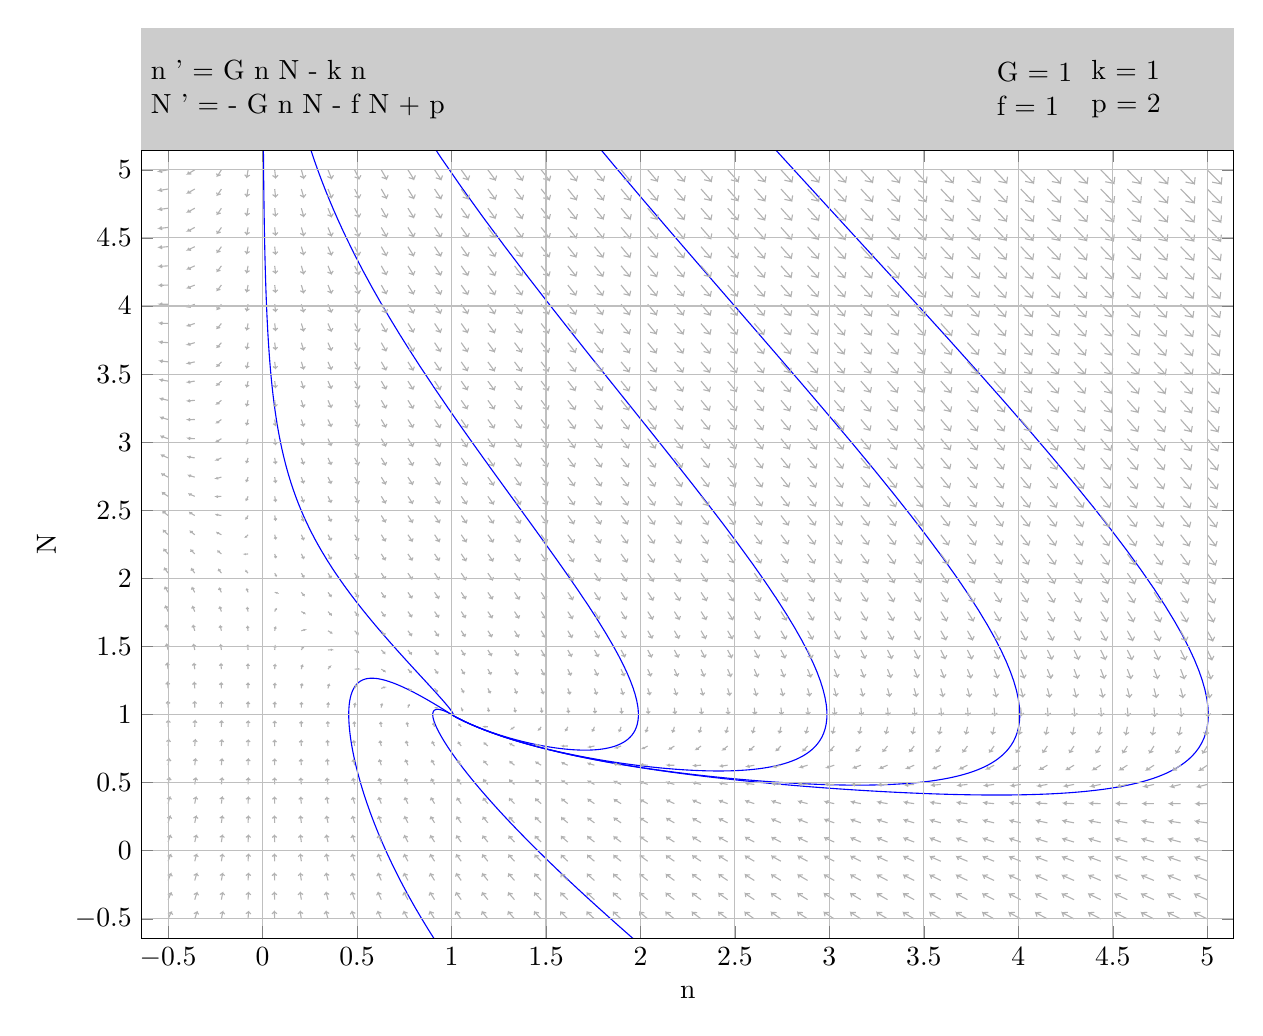
\begin{tikzpicture}

\begin{axis}[%
width=5.4625in,
height=0.614583in,
at={(0.552083in,5.21875in)},
scale only axis,
every outer x axis line/.append style={black},
every x tick label/.append style={font=\color{black}},
xmin=0,
xmax=1,
xtick={-1},
xticklabels={\empty},
every outer y axis line/.append style={black},
every y tick label/.append style={font=\color{black}},
ymin=0,
ymax=1,
ytick={-1},
yticklabels={\empty},
hide axis,
axis background/.style={fill=white!80!black},
axis x line*=bottom,
axis y line*=left
]
\node[right, align=left, inner sep=0mm, text=black]
at (axis cs:0.00806451612903225,0.495614035087719,0) {n ' = G n N - k n\\N ' = - G n N - f N + p};
\node[right, align=left, inner sep=0mm, text=black]
at (axis cs:0.869047619047619,0.5,0) {k = 1\\p = 2};
\node[right, align=left, inner sep=0mm, text=black]
at (axis cs:0.782380952380952,0.5,0) {G = 1\\f = 1};
\node[right, align=left, inner sep=0mm, text=black]
at (axis cs:0.7,0.5,0) { \\ };
\end{axis}

\begin{axis}[%
width=5.4625in,
height=3.9375in,
at={(0.552083in,1.28125in)},
scale only axis,
unbounded coords=jump,
separate axis lines,
every outer x axis line/.append style={black},
every x tick label/.append style={font=\color{black}},
xmin=-0.641025641025641,
xmax=5.14102564102564,
xlabel={n},
xmajorgrids,
every outer y axis line/.append style={black},
every y tick label/.append style={font=\color{black}},
ymin=-0.641025641025641,
ymax=5.14102564102564,
ylabel={N},
ymajorgrids,
every outer z axis line/.append style={black},
every z tick label/.append style={font=\color{black}},
zmin=-50,
zmax=50,
view={0}{90}
]
\addplot3 [color=blue,solid]
 table[row sep=crcr] {%
1.31832899202483e-06	12.1243668853552	-6.10362044133528\\
1.58703349163412e-06	11.944995644295	-6.08574486165555\\
1.89120267919303e-06	11.7688022812782	-6.06786928197581\\
2.26015335563121e-06	11.5957304408029	-6.04999370229607\\
2.71755736709851e-06	11.4257247571218	-6.03211812261633\\
3.281441604965e-06	11.2587308542417	-6.01424254293659\\
3.96418800582093e-06	11.0946953459238	-5.99636696325685\\
4.77253355147678e-06	10.9335658356836	-5.97849138357711\\
5.70757026896321e-06	10.7752909167908	-5.96061580389737\\
6.68509053515054e-06	10.6310372715596	-5.9440406963155\\
7.79776142265315e-06	10.4891548132063	-5.92746558873364\\
9.08648894897999e-06	10.3496045049574	-5.91089048115177\\
1.0587389805895e-05	10.2123479478841	-5.89431537356991\\
1.23317913594171e-05	10.0773473809026	-5.87774026598804\\
1.43462316498202e-05	9.94456568077369	-5.86116515840618\\
1.66524593916333e-05	9.81396636210293	-5.84459005082431\\
1.92674339736403e-05	9.68551357734075	-5.82801494324245\\
2.20383260202277e-05	9.56598780889681	-5.81234105946999\\
2.51466025405138e-05	9.44832050430173	-5.79666717569754\\
2.86517389528973e-05	9.33248268637739	-5.78099329192509\\
3.26093656913795e-05	9.21844582633287	-5.76531940815264\\
3.70712682055648e-05	9.10618184376444	-5.74964552438018\\
4.20853869606604e-05	8.99566310665562	-5.73397164060773\\
4.76958174374766e-05	8.88686243137712	-5.71829775683528\\
5.39428101324266e-05	8.77975308268687	-5.70262387306283\\
6.05933177596043e-05	8.67825881563576	-5.68754160321869\\
6.79453632848276e-05	8.57828303797706	-5.67245933337455\\
7.6085870666939e-05	8.47980291427028	-5.65737706353041\\
8.50988105593075e-05	8.38279594883738	-5.64229479368627\\
9.50652003098285e-05	8.28723998576272	-5.62721252384213\\
0.000106063103960924	8.19311320889308	-5.61213025399799\\
0.000118167632249542	8.10039414183765	-5.59704798415385\\
0.000131450942607158	8.00906164796807	-5.58196571430971\\
0.000145667228884875	7.92098140010143	-5.56720204736658\\
0.000161196423730633	7.83419047621957	-5.55243838042345\\
0.00017816476084985	7.74866982940405	-5.53767471348032\\
0.000196696227635576	7.66440068933203	-5.5229110465372\\
0.000216912565168495	7.58136456227632	-5.50814737959407\\
0.000238933268216918	7.49954323110529	-5.49338371265094\\
0.000262875585236792	7.41891875528294	-5.47862004570781\\
0.000288854518371693	7.33947347086889	-5.46385637876469\\
0.000316899683103717	7.26142691677659	-5.44913773007106\\
0.000347252956731271	7.1845179807311	-5.43441908137744\\
0.000380097338302613	7.10872981906924	-5.41970043268382\\
0.000415613959158328	7.03404583085422	-5.40498178399019\\
0.000453982082931337	6.96044965787572	-5.39026313529657\\
0.000495379105546889	6.88792518464984	-5.37554448660295\\
0.000539980555222567	6.81645653841912	-5.36082583790932\\
0.000587960092468285	6.74602808915251	-5.3461071892157\\
0.000640420163989324	6.6754321813923	-5.33113380466257\\
0.000696806788433233	6.60588076098866	-5.31616042010943\\
0.000757387871969513	6.53735797352776	-5.3011870355563\\
0.00082242927108558	6.46984819578727	-5.28621365100316\\
0.000892194792586772	6.40333603573636	-5.27124026645003\\
0.000966946193596348	6.33780633253566	-5.25626688189689\\
0.00104694318155548	6.27324415653732	-5.24129349734376\\
0.00113244341422327	6.20963480928498	-5.22632011279062\\
0.00122746007154908	6.14449159730713	-5.21075148461216\\
0.00132908086840646	6.08034665881703	-5.1951828564337\\
0.00143770638463373	6.01718406439352	-5.17961422825523\\
0.00155373390591094	5.95498812506442	-5.16404560007677\\
0.00167755742375987	5.8937433923066	-5.14847697189831\\
0.00180956763554402	5.83343465804591	-5.13290834371984\\
0.00195015194446863	5.77404695465724	-5.11733971554138\\
0.00209969445958067	5.71556555496445	-5.10177108736292\\
0.00226893865466355	5.65436901010245	-5.08521936769883\\
0.00244931970965511	5.59416313213843	-5.06866764803474\\
0.00264145323406602	5.53493085408755	-5.05211592837065\\
0.00284594806056321	5.47665538244491	-5.03556420870656\\
0.00306340624496991	5.41932019718548	-5.01901248904247\\
0.00329442306626558	5.36290905176419	-5.00246076937838\\
0.00353958702658598	5.30740597311583	-4.9859090497143\\
0.00379947985122312	5.25279526165514	-4.96935733005021\\
0.00409914625525197	5.19446938364262	-4.95137861150394\\
0.00441778640841195	5.13715846032978	-4.93339989295768\\
0.00475637278723727	5.08084308876923	-4.91542117441141\\
0.0051158626059272	5.02550420509032	-4.89744245586515\\
0.00549719781634609	4.97112308449918	-4.87946373731888\\
0.00590130510802332	4.91768134127864	-4.86148501877262\\
0.00632909590815335	4.86516092878833	-4.84350630022635\\
0.00678146638159572	4.8135441394646	-4.82552758168009\\
0.00731282666127423	4.75735102875201	-4.80559429314019\\
0.00787696755087658	4.70222369306849	-4.78566100460029\\
0.00847546214203873	4.64813886774216	-4.76572771606039\\
0.00910984818337781	4.59507374463868	-4.74579442752049\\
0.00978162808049216	4.54300597216125	-4.72586113898059\\
0.0104922688959613	4.49191365525061	-4.70592785044069\\
0.0112432023493459	4.44177535538504	-4.68599456190079\\
0.012035824817188	4.39257009058039	-4.66606127336089\\
0.0129854912788782	4.33794842621179	-4.64348789877104\\
0.0139928142215429	4.28446711997665	-4.62091452418119\\
0.0150603898849957	4.23209682033674	-4.59834114959135\\
0.0161907306744933	4.18080884527763	-4.5757677750015\\
0.0173862651607348	4.13057518230869	-4.55319440041166\\
0.0186493380798622	4.0813684884631	-4.53062102582181\\
0.0199822103334599	4.03316209029783	-4.50804765123197\\
0.0213870589885553	3.98592998389364	-4.48547427664212\\
0.0231145048828484	3.93218214989271	-4.45921716336485\\
0.0249462969332755	3.87967814590093	-4.43296005008758\\
0.0268868165061369	3.82837862946247	-4.40670293681031\\
0.0289402336577782	3.77824535380167	-4.38044582353304\\
0.0311105071345899	3.72924116782305	-4.35418871025577\\
0.033401384373008	3.68133001611129	-4.32793159697849\\
0.0358164014995134	3.63447693893127	-4.30167448370122\\
0.0383588833306323	3.58864807222803	-4.27541737042395\\
0.0415833034762917	3.53494657016423	-4.24390139474907\\
0.0450028181097616	3.48261608713717	-4.21238541907418\\
0.0486247600255952	3.4316006677304	-4.1808694433993\\
0.0524558814741937	3.38184639872451	-4.14935346772442\\
0.0565023541618064	3.33330140909703	-4.11783749204953\\
0.0607697692505307	3.28591587002255	-4.08632151637465\\
0.065263137358312	3.23964199487261	-4.05480554069977\\
0.0699868885589437	3.19443403921577	-4.02328956502488\\
0.074757449597025	3.15186822970086	-3.99294234277684\\
0.0797508748377081	3.1102093643886	-3.9625951205288\\
0.0849717085821018	3.06941910364036	-3.93224789828076\\
0.0904239688719805	3.02946061454996	-3.90190067603272\\
0.0961111474897835	2.99029857094371	-3.87155345378468\\
0.102036209958615	2.95189915338038	-3.84120623153664\\
0.108201595542246	2.91423004915122	-3.8108590092886\\
0.114609217245112	2.87726045227996	-3.78051178704055\\
0.122534803559731	2.83422792834621	-3.74447546814633\\
0.130807190121676	2.79209129865497	-3.7084391492521\\
0.139428662253288	2.75080426185314	-3.67240283035787\\
0.148400246356396	2.71032327486105	-3.63636651146365\\
0.157721709912322	2.67060755287242	-3.60033019256942\\
0.167391561481878	2.6316190693544	-3.56429387367519\\
0.177407050705367	2.59332255604754	-3.52825755478097\\
0.187764168302583	2.55568550296579	-3.49222123588674\\
0.20147473196144	2.50854825680279	-3.44621745575532\\
0.215722620749614	2.4623767969206	-3.40021367562389\\
0.230493083510215	2.41711826237871	-3.35420989549247\\
0.245768121510955	2.37272591837528	-3.30820611536105\\
0.261526488444154	2.32915915624708	-3.26220233522962\\
0.277743690426742	2.28638349346953	-3.2161985550982\\
0.294391986000251	2.2443705736567	-3.17019477496678\\
0.311440386130823	2.20309816656128	-3.12419099483536\\
0.340805357783479	2.13557573282343	-3.04713955702428\\
0.371031601592123	2.07002254346237	-2.97008811921321\\
0.401925559273477	2.00642291686946	-2.89303668140213\\
0.433290289382802	1.94477842784529	-2.81598524359106\\
0.464925467313904	1.88510790759963	-2.73893380577998\\
0.496627385299129	1.82744744375151	-2.66188236796891\\
0.528188952409367	1.77185038032913	-2.58483093015783\\
0.559399694554047	1.71838731776994	-2.50777949234676\\
0.58933787968748	1.66832385248644	-2.43257315880492\\
0.618595782871089	1.62039912745321	-2.35736682526308\\
0.647022090197248	1.57465909335513	-2.28216049172123\\
0.674485673026829	1.53113636492016	-2.20695415817939\\
0.700875587989203	1.48985022091932	-2.13174782463755\\
0.72610107698224	1.4508066041667	-2.05654149109571\\
0.750091567172308	1.41399812151946	-1.98133515755387\\
0.772796670994272	1.37940404387783	-1.90612882401203\\
0.804503743416373	1.33139649267725	-1.79286272101053\\
0.83321609966911	1.28812974896091	-1.67959661800902\\
0.8589804375034	1.24937249140385	-1.56633051500752\\
0.881883966146493	1.21486935208617	-1.45306441200602\\
0.902054406301979	1.18434091649296	-1.33979830900451\\
0.91965999014978	1.15748372351439	-1.22653220600301\\
0.934909461346158	1.13397026544562	-1.1132661030015\\
0.948052075023708	1.11344898798687	-1\\
0.960388969405012	1.09388426581846	-0.875\\
0.970693561147213	1.07720132552406	-0.75\\
0.979224575807999	1.06304328768415	-0.625\\
0.986220114923572	1.05108328697185	-0.5\\
0.991897656008655	1.04102447215298	-0.375\\
0.996454052556492	1.03260000608604	-0.25\\
1.00006553403884	1.02557306572218	-0.125\\
1.00288770590599	1.01973684210526	0\\
1.00288770590599	1.01973684210526	0\\
1.00450729885488	1.01617300543092	0.0898082466620046\\
1.00583319877818	1.01306905994306	0.179616493324009\\
1.0068980386443	1.01037923889832	0.269424739986014\\
1.00773312096139	1.00805970704373	0.359232986648019\\
1.00836841777728	1.00606856061665	0.449041233310023\\
1.00883257067958	1.00436582734483	0.538849479972028\\
1.00915289079559	1.00291346644638	0.628657726634033\\
1.00935535879233	1.00167536862979	0.718465973296037\\
1.00946235163819	1.00059388697638	0.810904177835926\\
1.00947915741713	0.999688176148131	0.903342382375816\\
1.00941814748886	0.998938958830586	0.995780586915705\\
1.00929126621889	0.998327696567781	1.08821879145559\\
1.00911003097851	0.997836589762233	1.18065699599548\\
1.00888553214483	0.997448577674947	1.27309520053537\\
1.00862843310076	0.997147338425412	1.36553340507526\\
1.00834897023503	0.996917288991602	1.45797160961515\\
1.00800185243819	0.996720706811963	1.56680831872373\\
1.00763971630944	0.996594662649635	1.67564502783231\\
1.00726663851813	0.996530110148907	1.78448173694088\\
1.00688694997725	0.996517932479422	1.89331844604946\\
1.00650523584337	0.996548942336182	2.00215515515804\\
1.00612633551672	0.996613881939543	2.11099186426662\\
1.00575534264113	0.996703423035219	2.2198285733752\\
1.00539760510403	0.996808166894282	2.32866528248377\\
1.00500655466998	0.996939466942569	2.45366528248377\\
1.00463468253775	0.997081604815716	2.57866528248377\\
1.00428093654481	0.997232783913105	2.70366528248377\\
1.00394483398557	0.997390692029029	2.82866528248377\\
1.00362646161139	0.99755250135269	2.95366528248377\\
1.00332647563057	0.9977148684682	3.07866528248377\\
1.00304610170836	0.997873934354582	3.20366528248377\\
1.00278713496695	0.998025324385765	3.32866528248377\\
1.00254910901061	0.998167675616683	3.45366528248377\\
1.00232901388384	0.998303151958023	3.57866528248377\\
1.00212542841041	0.998432125291588	3.70366528248377\\
1.00193716067879	0.998554758069919	3.82866528248377\\
1.00176324804214	0.998671003316301	3.95366528248377\\
1.00160295711829	0.998780604624757	4.07866528248377\\
1.0014557837898	0.998883096160052	4.20366528248377\\
1.00132145320389	0.998977802657694	4.32866528248377\\
1.00119913253601	0.999064883135039	4.45366528248377\\
1.00108741102507	0.999145436726683	4.57866528248377\\
1.00098538732475	0.999219978288818	4.70366528248377\\
1.00089225137243	0.999288938700016	4.82866528248377\\
1.00080728438913	0.999352664861223	4.95366528248377\\
1.00072985887959	0.999411419695763	5.07866528248377\\
1.0006594386322	0.999465382149333	5.20366528248377\\
1.00059557871901	0.999514647190009	5.32866528248377\\
1.00053772924387	0.999559516528298	5.45366528248377\\
1.00048525885675	0.999600506731809	5.57866528248377\\
1.00043769604632	0.999637946954679	5.70366528248377\\
1.0003946054808	0.999672132862553	5.82866528248377\\
1.00035558800797	0.999703326632581	5.95366528248377\\
1.00032028065517	0.999731756953423	6.07866528248377\\
1.00028835662929	0.999757619025242	6.20366528248377\\
1.00025952531678	0.999781074559712	6.32866528248377\\
1.00023349429668	0.999802324562731	6.45366528248377\\
1.00020998947938	0.999821600845745	6.57866528248377\\
1.00018878559698	0.999839076241724	6.70366528248377\\
1.00016967166702	0.999854910289446	6.82866528248377\\
1.00015245099244	0.999869249233494	6.95366528248377\\
1.00013694116157	0.999882226024259	7.07866528248377\\
1.00012297404815	0.999893960317936	7.20366528248377\\
1.00011039581131	0.999904558476525	7.32866528248377\\
1.0000990655281	0.99991412775178	7.45366528248377\\
1.00008886685945	0.9999227689103	7.57866528248377\\
1.00007969776887	0.999930564675056	7.70366528248377\\
1.00007146183915	0.999937592514811	7.82866528248377\\
1.00006406827243	0.999943924644124	7.95366528248377\\
1.0000574318901	0.999949628023346	8.07866528248377\\
1.00005147313288	0.999954764358624	8.20366528248377\\
1.00004611806079	0.999959390101897	8.32866528248377\\
1.00004130250672	0.999963557018041	8.45366528248377\\
1.00003697794056	0.999967307901303	8.57866528248377\\
1.00003309974401	0.99997068025617	8.70366528248377\\
1.00002962550106	0.99997370951932	8.82866528248377\\
1.00002651499798	0.999976429059616	8.95366528248377\\
1.00002373022334	0.999978870178114	9.07866528248377\\
1.00002123536798	0.999981062108054	9.20366528248377\\
1.00001899682505	0.999983032014869	9.32866528248377\\
1.00001698643825	0.9999848034867	9.45366528248377\\
1.00001518423912	0.999986394379302	9.57866528248377\\
1.00001357119935	0.999987821100717	9.70366528248377\\
1.00001212915079	0.999989099248382	9.82866528248377\\
1.00001084078541	0.999990243609133	9.95366528248377\\
1.00000968965533	0.999991268159205	10.0786652824838\\
1.00000866017278	0.999992186064229	10.2036652824838\\
1.00000773761014	0.999993009679232	10.3286652824838\\
1.00000690993008	0.999993749358943	10.4536652824838\\
1.00000616900639	0.99999441245139	10.5786652824838\\
1.00000550687439	0.999995005956131	10.7036652824838\\
1.00000491590427	0.99999553655609	10.8286652824838\\
1.0000043888011	0.999996010617563	10.9536652824838\\
1.00000391860481	0.999996434190215	11.0786652824838\\
1.00000349869022	0.999996813007078	11.2036652824838\\
1.00000312276703	0.999997152484555	11.3286652824838\\
1.0000027857875	0.999997457050626	11.4536652824838\\
1.00000248447442	0.999997729695869	11.5786652824838\\
1.00000221554193	0.999997973350644	11.7036652824838\\
1.0000019758342	0.999998190822033	11.8286652824838\\
1.00000176232537	0.999998384793835	11.9536652824838\\
1.0000015721196	0.999998557826568	12.0786652824838\\
1.00000140245104	0.999998712357466	12.2036652824838\\
1.00000125068385	0.999998850700486	12.3286652824838\\
1.00000111473259	0.999998974712783	12.4536652824838\\
1.00000099328554	0.999999085600513	12.5786652824838\\
1.00000088500267	0.999999184572765	12.7036652824838\\
1.00000078859428	0.999999272790768	12.8286652824838\\
1.00000070282102	0.999999351367891	12.9536652824838\\
1.00000062649386	0.999999421369641	13.0786652824838\\
1.00000055847414	0.999999483813664	13.2036652824838\\
1.00000049767348	0.999999539669745	13.3286652824838\\
1.00000044324046	0.999999589705255	13.4536652824838\\
1.00000039465337	0.999999634402996	13.5786652824838\\
1.00000035137085	0.999999674256106	13.7036652824838\\
1.00000031287097	0.999999709739192	13.8286652824838\\
1.00000027865125	0.999999741308329	13.9536652824838\\
1.00000024822867	0.999999769401057	14.0786652824838\\
1.00000022113962	0.999999794436388	14.2036652824838\\
1.00000019693996	0.999999816814799	14.3286652824838\\
1.00000017528538	0.999999836849627	14.4536652824838\\
1.00000015596953	0.999999854732898	14.5786652824838\\
1.0000001387754	0.999999870663855	14.7036652824838\\
1.00000012349349	0.999999884834582	14.8286652824838\\
1.00000010992177	0.999999897430004	14.9536652824838\\
1.00000009786573	0.999999908627887	15.0786652824838\\
1.00000008713832	0.999999918598838	15.2036652824838\\
1.00000007756003	0.999999927506307	15.3286652824838\\
1.00000006899272	0.999999935477009	15.4536652824838\\
1.00000006135516	0.999999942586904	15.5786652824838\\
1.00000005456093	0.999999948915861	15.7036652824838\\
1.00000004852651	0.999999954540994	15.8286652824838\\
1.00000004317125	0.999999959536655	15.9536652824838\\
1.00000003841738	0.999999963974438	16.0786652824838\\
1.00000003419001	0.999999967923176	16.2036652824838\\
1.00000003041715	0.999999971448946	16.3286652824838\\
1.00000002704377	0.999999974602583	16.4536652824838\\
1.000000024038	0.999999977413992	16.5786652824838\\
1.00000002136564	0.99999997991498	16.7036652824838\\
1.00000001899357	0.999999982136293	16.8286652824838\\
1.0000000168898	0.999999984107616	16.9536652824838\\
1.00000001502341	0.999999985857573	17.0786652824838\\
1.00000001336463	0.999999987413723	17.2036652824838\\
1.00000001188478	0.999999988802569	17.3286652824838\\
1.00000001056204	0.999999990044367	17.4536652824838\\
1.00000000938397	0.999999991150843	17.5786652824838\\
1.0000000083371	0.999999992134592	17.7036652824838\\
1.00000000740837	0.999999993007801	17.8286652824838\\
1.00000000658513	0.99999999378225	17.9536652824838\\
1.00000000585518	0.999999994469313	18.0786652824838\\
1.00000000520674	0.999999995079954	18.2036652824838\\
1.00000000462844	0.999999995624731	18.3286652824838\\
1.00000000411169	0.999999996111671	18.4536652824838\\
1.00000000365164	0.999999996545352	18.5786652824838\\
1.000000003243	0.999999996930739	18.7036652824838\\
1.00000000288065	0.999999997272639	18.8286652824838\\
1.00000000255962	0.999999997575702	18.9536652824838\\
1.0000000022751	0.999999997844422	19.0786652824838\\
1.00000000202246	0.999999998083139	19.2036652824838\\
1.00000000179722	0.999999998296034	19.3286652824838\\
1.000000001596	0.999999998486273	19.4536652824838\\
1.00000000141692	0.999999998655636	19.5786652824838\\
1.00000000125792	0.999999998806073	19.7036652824838\\
1.00000000111699	0.999999998939472	19.8286652824838\\
1.00000000099218	0.999999999057659	19.9536652824838\\
1.00000000088162	0.999999999162403	20.0786652824838\\
1.00000000078348	0.999999999255413	20.2036652824838\\
1.00000000069601	0.999999999338336	20.3286652824838\\
};
 \addplot3 [color=blue,solid]
 table[row sep=crcr] {%
0.000112261169607266	12.0941948852517	-2.31936719275377\\
0.000124085642560025	12.0029861161647	-2.31029164140616\\
0.000137029221612918	11.9126001477513	-2.30121609005855\\
0.000151207267973945	11.8230294198531	-2.29214053871094\\
0.000166736153948131	11.7342664381906	-2.28306498736333\\
0.000183733262937528	11.646303774364	-2.27398943601573\\
0.000202316989441213	11.5591340658526	-2.26491388466812\\
0.00022260673905529	11.4727500160155	-2.25583833332051\\
0.000244722928472889	11.3871443940908	-2.2467627819729\\
0.000267786472757775	11.3057022174625	-2.23805170675467\\
0.000292801770320649	11.2249642581421	-2.22934063153645\\
0.000319937858759879	11.144924221472	-2.22062955631822\\
0.000349366578794048	11.0655758628438	-2.21191848109999\\
0.000381262574261959	10.9869129876985	-2.20320740588176\\
0.000415803292122635	10.9089294515261	-2.19449633066353\\
0.000453168982455314	10.8316191598662	-2.1857852554453\\
0.000493542698459453	10.7549760683074	-2.17707418022707\\
0.0005360528239811	10.6807743205321	-2.16856805862851\\
0.00058184106349386	10.6071974279021	-2.16006193702995\\
0.000631156008801838	10.5342398208043	-2.15155581543139\\
0.000684251186662079	10.4618959695321	-2.14304969383283\\
0.000741385058784567	10.3901603842861	-2.13454357223427\\
0.000802821021832224	10.3190276151736	-2.12603745063571\\
0.000868827407420911	10.2484922522088	-2.11753132903716\\
0.000939677482119428	10.1785489253127	-2.1090252074386\\
0.0010152072003623	10.10958649512	-2.10056763472075\\
0.00109614884512377	10.0411988130867	-2.0921100620029\\
0.00118287344636957	9.97338062148866	-2.08365248928505\\
0.00127575970548348	9.906126695879	-2.07519491656721\\
0.00137519399526734	9.83943184508877	-2.06673734384936\\
0.00148157035994102	9.77329091122665	-2.05827977113151\\
0.00159529051514245	9.70769876967899	-2.04982219841366\\
0.00171676384792762	9.64265032910989	-2.04136462569582\\
0.00184807268814529	9.57734524553747	-2.03280234831718\\
0.00198828734838261	9.51258691079248	-2.02424007093855\\
0.00213797412606189	9.44837002058511	-2.01567779355991\\
0.00229771072013724	9.38468929941318	-2.00711551618127\\
0.00246808623109462	9.32153950056218	-1.99855323880264\\
0.00264970116095184	9.25891540610525	-1.989990961424\\
0.00284316741325856	9.19681182690318	-1.98142868404537\\
0.00304910829309625	9.13522360260441	-1.97286640666673\\
0.00327482898513027	9.0723529960039	-1.96405175484503\\
0.00351527536619222	9.01001743101872	-1.95523710302333\\
0.00377133334817564	8.94821119634666	-1.94642245120163\\
0.00404390542784378	8.88692860622396	-1.93760779937993\\
0.00433391068682955	8.82616400042532	-1.92879314755823\\
0.00464228479163554	8.76591174426389	-1.91997849573653\\
0.00496997999363405	8.70616622859124	-1.91116384391483\\
0.00531796512906704	8.64692186979743	-1.90234919209313\\
0.00570427922998943	8.58555465628472	-1.89313994427387\\
0.00611514721205252	8.52472190028098	-1.88393069645462\\
0.00655198681429412	8.46441705882852	-1.87472144863536\\
0.00701623929662734	8.40463361216847	-1.86551220081611\\
0.00750936943984054	8.34536506374069	-1.85630295299685\\
0.00803286554559741	8.28660494018385	-1.8470937051776\\
0.0085882394364369	8.22834679133536	-1.83788445735835\\
0.00917702645577329	8.17058419023143	-1.82867520953909\\
0.0098383306856951	8.10998164411449	-1.81892825696544\\
0.0105409797604125	8.0499191609357	-1.80918130439179\\
0.0112872860653547	7.99038878794282	-1.79943435181813\\
0.0120795935439366	7.93138259520479	-1.78968739924448\\
0.0129202776975591	7.87289267561172	-1.77994044667083\\
0.0138117455856092	7.81491114487492	-1.77019349409717\\
0.0147564358254596	7.75743014152687	-1.76044654152352\\
0.0157568185924691	7.70044182692122	-1.75069958894987\\
0.0168933996089949	7.6399163514103	-1.7402556618344\\
0.0181003890560253	7.57993749488428	-1.72981173471894\\
0.0193816196057739	7.52049501281529	-1.71936780760348\\
0.0207409603909009	7.46157869039084	-1.70892388048801\\
0.0221823170045135	7.4031783425138	-1.69847995337255\\
0.0237096315001655	7.34528381380238	-1.68803602625708\\
0.0253268823918573	7.28788497859018	-1.67759209914162\\
0.0270380846540364	7.23097174092616	-1.66714817202615\\
0.0290085776923177	7.16967279629663	-1.6558005882559\\
0.0311008144936208	7.10892153959017	-1.64445300448566\\
0.033321250359564	7.04870396038945	-1.63310542071541\\
0.0356763617908783	6.98900611169547	-1.62175783694516\\
0.038172646487408	6.92981410992754	-1.61041025317492\\
0.0408166233481102	6.87111413492329	-1.59906266940467\\
0.0436148324710549	6.81289242993866	-1.58771508563442\\
0.0465738351534251	6.75513530164792	-1.57636750186418\\
0.0500504105355233	6.69162622488114	-1.56378637042847\\
0.0537431368288692	6.62865154646937	-1.55120523899276\\
0.0576631446524082	6.56619074981022	-1.53862410755705\\
0.061821483549383	6.50422351572577	-1.52604297612135\\
0.0662291219873324	6.44272972246251	-1.51346184468564\\
0.0708969473580925	6.3816894456914	-1.50088071324993\\
0.0758357659777958	6.32108295850783	-1.48829958181423\\
0.0810563030868717	6.26089073143162	-1.47571845037852\\
0.0874609100518712	6.19174886820034	-1.4611639378306\\
0.0942757618502702	6.12310326423784	-1.44660942528267\\
0.101521324828836	6.05492035087344	-1.43205491273475\\
0.109217464694875	5.98716734742647	-1.41750040018683\\
0.117383446516234	5.91981226120624	-1.4029458876389\\
0.126037934721299	5.85282388751212	-1.38839137509098\\
0.135198993098996	5.78617180963346	-1.37383686254306\\
0.14488408479879	5.71982639884961	-1.35928234999514\\
0.157717294079608	5.63749698847511	-1.34113644933664\\
0.171428378461427	5.55553941827229	-1.32299054867814\\
0.18605777549335	5.47389076827985	-1.30484464801964\\
0.20164224628364	5.39249219354831	-1.28669874736114\\
0.21821487549972	5.31128892413995	-1.26855284670264\\
0.235805071368173	5.23023026512885	-1.25040694604414\\
0.254438565674743	5.14926959660091	-1.23226104538564\\
0.274137413764334	5.06836437365379	-1.21411514472714\\
0.29278931123708	4.99558365002181	-1.19778848032062\\
0.312337941374564	4.92278277061883	-1.18146181591411\\
0.332796831487053	4.84993400744282	-1.1651351515076\\
0.354175749707158	4.77701361883463	-1.14880848710108\\
0.376480704989834	4.70400184947807	-1.13248182269457\\
0.399713947112378	4.63088293039984	-1.11615515828805\\
0.423873966674433	4.55764507896955	-1.09982849388154\\
0.448955495097982	4.48428049889975	-1.08350182947503\\
0.490108336216074	4.3690031931486	-1.05790649373144\\
0.533453204397082	4.2534070882184	-1.03231115798786\\
0.578914455227355	4.13752046106247	-1.00671582224428\\
0.626389104214135	4.02140009812574	-0.981120486500692\\
0.675746826785556	3.90513129534474	-0.955525150757108\\
0.726829958290646	3.7888278581476	-0.929929815013524\\
0.779453493999323	3.67263210145404	-0.904334479269941\\
0.833405089102401	3.55671484967536	-0.878739143526357\\
0.907492036703761	3.4019402358099	-0.844397291336663\\
0.982941587289721	3.24852712631502	-0.810055439146968\\
1.05906875221526	3.09706848099064	-0.775713586957274\\
1.13519819625609	2.94815060393503	-0.741371734767579\\
1.21066423760865	2.80235314354479	-0.707029882577885\\
1.28481084789008	2.6602490925148	-0.67268803038819\\
1.35699165213829	2.52240478783833	-0.638346178198496\\
1.42656992881189	2.38937991080692	-0.604004326008802\\
1.49557629371593	2.25665750873438	-0.568287067516998\\
1.56068253851665	2.13007099141639	-0.532569809025194\\
1.62147139617637	2.0099591239746	-0.49685255053339\\
1.67762171747637	1.89656720583319	-0.461135292041586\\
1.72890847101686	1.79004707071886	-0.425418033549782\\
1.77520274321699	1.69045708666084	-0.389700775057978\\
1.81647173831485	1.59776215599087	-0.353983516566174\\
1.85277877836746	1.51183371534324	-0.31826625807437\\
1.88194479133373	1.43849244784379	-0.285358655694106\\
1.90713706892416	1.37055504587164	-0.252451053313841\\
1.92852734588281	1.30780344515218	-0.219543450933577\\
1.94630081404243	1.25000757456381	-0.186635848553312\\
1.9606561223244	1.19692535613792	-0.153728246173048\\
1.9718053767388	1.14830270505892	-0.120820643792784\\
1.97997414038435	1.10387352966425	-0.0879130414125193\\
1.98540143344845	1.06335973144432	-0.0550054390322549\\
1.98621175901112	1.05536319322888	-0.0481297591532231\\
1.98691424329341	1.04752373696045	-0.0412540792741912\\
1.98751090486901	1.03983900663286	-0.0343783993951593\\
1.98800374765961	1.03230666319522	-0.0275027195161275\\
1.98839476093487	1.02492438455189	-0.0206270396370956\\
1.98868591931243	1.01768986556249	-0.0137513597580637\\
1.98887918275793	1.01060081804189	-0.00687567987903187\\
1.98897649658497	1.00365497076023	0\\
1.98897649658497	1.00365497076023	0\\
1.9889797916201	0.996850069076906	0.00687567987903187\\
1.98889098021944	0.990183879045216	0.0137513597580637\\
1.98871195509188	0.983654188701979	0.0206270396370956\\
1.98844459039944	0.977258806763182	0.0275027195161275\\
1.98809074175729	0.970995562623988	0.0343783993951593\\
1.98765224623379	0.964862306358731	0.0412540792741912\\
1.98713092235041	0.958856908720916	0.0481297591532231\\
1.98652857008181	0.952977261143223	0.0550054390322549\\
1.98272446360842	0.927259229790391	0.0869326023462139\\
1.97738634679614	0.904002754789431	0.118859765660173\\
1.97067166419191	0.883021451021432	0.150786928974132\\
1.9627289037187	0.864138683663121	0.182714092288091\\
1.95369759667547	0.847187568186861	0.21464125560205\\
1.9437083177372	0.832010970360656	0.246568418916009\\
1.93288268495489	0.818461506248143	0.278495582229968\\
1.92133335975553	0.806401542208602	0.310422745543927\\
1.9094376638226	0.795924544041333	0.341647978510829\\
1.89703300221817	0.786644224207747	0.372873211477732\\
1.88419477970821	0.778464177771647	0.404098444444635\\
1.87099313518346	0.771293831127753	0.435323677411537\\
1.8574929416595	0.765048442001705	0.46654891037844\\
1.8437538062767	0.75964909945006	0.497774143345343\\
1.82983007030024	0.755022723860293	0.528999376312245\\
1.81577080912011	0.751102066950799	0.560224609279148\\
1.79996468015675	0.747481857366976	0.595094586407533\\
1.78409585699379	0.744589944266101	0.629964563535918\\
1.76820830807233	0.74235974517567	0.664834540664303\\
1.75234227216758	0.740729073385017	0.699704517792689\\
1.73653425838879	0.73964013794531	0.734574494921074\\
1.72081704617931	0.739039543669556	0.769444472049459\\
1.70521968531656	0.738878291132595	0.804314449177844\\
1.68976749591202	0.739111776671108	0.839184426306229\\
1.67230668280306	0.739810472915449	0.879051641101276\\
1.65508810169105	0.740921866984267	0.918918855896323\\
1.63813069139798	0.74240171939341	0.95878607069137\\
1.62145124810176	0.744208760310178	0.998653285486417\\
1.60506442533623	0.746304689553324	1.03852050028146\\
1.58898273399113	0.74865417659305	1.07838771507651\\
1.5732165423121	0.751224860551008	1.11825492987156\\
1.55777407590073	0.753987350200305	1.1581221446666\\
1.54025391789798	0.757401697231211	1.20442193840418\\
1.52318037063423	0.761007345043389	1.25072173214176\\
1.50655262240172	0.76477671206048	1.29702152587933\\
1.49036919968399	0.768683912769903	1.34332131961691\\
1.47462796715589	0.772704757722861	1.38962111335449\\
1.45932612768358	0.776816753534338	1.43592090709206\\
1.44446022232453	0.780999102883103	1.48222070082964\\
1.43002613032753	0.785232704511703	1.52852049456721\\
1.41378527248786	0.790195757430928	1.58233184666275\\
1.39810539049701	0.795188210372985	1.63614319875828\\
1.38297090892636	0.80019542035046	1.68995455085381\\
1.36836688413815	0.805203325751479	1.74376590294934\\
1.3542790042855	0.81019844633971	1.79757725504488\\
1.34069358931238	0.815167883254357	1.85138860714041\\
1.32759759095364	0.820099319010168	1.90519995923594\\
1.31497859273498	0.824981017497429	1.95901131133147\\
1.30098790165888	0.830541858220951	2.02112594576577\\
1.28758944446311	0.836017502508599	2.08324058020006\\
1.27475848293513	0.841403137007977	2.14535521463436\\
1.26247185463634	0.846693654307506	2.20746984906866\\
1.25070797290209	0.851883652936415	2.26958448350295\\
1.2394468268417	0.856967437364749	2.33169911793725\\
1.22866998133841	0.861939018003362	2.39381375237154\\
1.21836057704945	0.866792111203921	2.45592838680584\\
1.20708682679007	0.872208318437908	2.52718463229884\\
1.19637434585308	0.877465282791376	2.59844087779184\\
1.18619423186894	0.882565498260209	2.66969712328485\\
1.17651970422269	0.887510544369843	2.74095336877785\\
1.16732610405394	0.892301086175261	2.81220961427085\\
1.15859089425687	0.896936874260997	2.88346585976386\\
1.15029365948023	0.901416744741134	2.95472210525686\\
1.14241610612736	0.905738619259303	3.02597835074987\\
1.13387134824538	0.910502343888448	3.10772373076992\\
1.12582166234194	0.915066773924935	3.18946911078998\\
1.11823727672363	0.919439928292938	3.27121449081003\\
1.11109078888827	0.923628470555976	3.35295987083009\\
1.10435716552496	0.927637708916911	3.43470525085015\\
1.098013742514	0.93147159621795	3.5164506308702\\
1.09204022492698	0.935132729940647	3.59819601089026\\
1.08641868702669	0.938622352205899	3.67994139091032\\
1.08033442286411	0.9424472899744	3.77443898440136\\
1.07466370461137	0.946061228780177	3.8689365778924\\
1.06937766261442	0.949476438841087	3.96343417138344\\
1.06444987328953	0.952703484036451	4.05793176487448\\
1.05985635912327	0.95575122190706	4.15242935836552\\
1.05557558867257	0.958626803655171	4.24692695185656\\
1.05158847656464	0.961335674144507	4.3414245453476\\
1.04787838349705	0.96388157190026	4.43592213883864\\
1.04384988857866	0.966672746287972	4.54694523115198\\
1.04014915452366	0.969264809164166	4.65796832346532\\
1.03674921300078	0.971673091934695	4.76899141577867\\
1.03362552017189	0.97391091123992	4.88001450809201\\
1.03075595669206	0.9759895689547	4.99103760040535\\
1.02812082770954	0.977918352188403	5.1020606927187\\
1.02570286286572	0.979704533284895	5.21308378503204\\
1.0234872162952	0.98135336982255	5.32410687734538\\
1.02121508917225	0.983055472431459	5.44910687734538\\
1.01915597704013	0.984610430704467	5.57410687734538\\
1.01729032873663	0.986031544167888	5.69910687734538\\
1.01560028021668	0.987330543409298	5.82410687734538\\
1.01406965455231	0.988517590077533	5.94910687734538\\
1.01268396193264	0.989601276882693	6.07410687734538\\
1.01143039966394	0.990588627596138	6.19910687734538\\
1.01029785216955	0.991485097050489	6.32410687734538\\
1.00927498561901	0.992298004571689	6.44910687734538\\
1.00835075886574	0.993036534653515	6.57410687734538\\
1.00751623377161	0.99370732274822	6.69910687734538\\
1.00676310296495	0.994316417070624	6.82410687734538\\
1.00608368984054	0.994869278598118	6.94910687734538\\
1.00547094855965	0.995370781070664	7.07410687734538\\
1.00491846405	0.995825210990795	7.19910687734538\\
1.00442045200577	0.99623626762361	7.32410687734538\\
1.0039714989504	0.996607885769843	7.44910687734538\\
1.00356693278563	0.996944053660635	7.57410687734538\\
1.00320273558354	0.997247941067934	7.69910687734538\\
1.00287513106367	0.997522492149429	7.82410687734538\\
1.00258058459303	0.997770425448546	7.94910687734538\\
1.00231580318605	0.99799423389445	8.07410687734538\\
1.00207773550465	0.998196184802045	8.19910687734538\\
1.00186357185818	0.998378319871976	8.32410687734538\\
1.00167082390232	0.998542582802968	8.44910687734538\\
1.00149753082822	0.99869068251282	8.57410687734538\\
1.00134192572969	0.998824073503598	8.69910687734538\\
1.00120233536143	0.998944122522058	8.82410687734538\\
1.00107718013901	0.99905210855964	8.94910687734538\\
1.00096497413885	0.999149222852467	9.07410687734538\\
1.00086432509828	0.999236568881349	9.19910687734538\\
1.00077393441549	0.999315162371782	9.32410687734538\\
1.00069269530046	0.999385909502659	9.44910687734538\\
1.0006197945667	0.999449530680583	9.57410687734538\\
1.00055447159825	0.999506671452677	9.69910687734538\\
1.00049600222562	0.999557943094804	9.82410687734538\\
1.00044369872577	0.999603922611566	9.94910687734538\\
1.00039690982217	0.999645152736301	10.0741068773454\\
1.00035502068474	0.999682141931088	10.1991068773454\\
1.0003174529299	0.999715364386742	10.3241068773454\\
1.00028372720428	0.999745225564865	10.4491068773454\\
1.00025351015883	0.999772024640587	10.5741068773454\\
1.00022648038915	0.999796040634609	10.6991068773454\\
1.00020233067467	0.999817539185015	10.8241068773454\\
1.00018076797864	0.999836772547274	10.9491068773454\\
1.00016151344813	0.999853979594237	11.0741068773454\\
1.00014430241402	0.999869385816141	11.1991068773454\\
1.00012888439103	0.999883203320604	11.3241068773454\\
1.00011505611359	0.999895608156375	11.4491068773454\\
1.00010268231014	0.999906723007642	11.5741068773454\\
1.0000916292576	0.999916665986148	11.6991068773454\\
1.00008176874411	0.999925549987539	11.8241068773454\\
1.00007297806901	0.999933482691366	11.9491068773454\\
1.00006514004286	0.999940566561078	12.0741068773454\\
1.00005814298742	0.999946898844029	12.1991068773454\\
1.00005188073564	0.999952571571474	12.3241068773454\\
1.00004626852894	0.999957659477162	12.4491068773454\\
1.00004125194226	0.999962212349789	12.5741068773454\\
1.00003677604488	0.999966279369901	12.6991068773454\\
1.00003278804287	0.999969907689954	12.8241068773454\\
1.00002923727909	0.999973142434315	12.9491068773454\\
1.00002607523319	0.999976026699263	13.0741068773454\\
1.00002325552159	0.99997860155299	13.1991068773454\\
1.00002073389752	0.9999809060356	13.3241068773454\\
1.00001847548991	0.999982971325668	13.4491068773454\\
1.00001645855855	0.999984817455689	13.5741068773454\\
1.00001466077545	0.999986464635664	13.6991068773454\\
1.00001306063921	0.999987932289046	13.8241068773454\\
1.00001163747503	0.999989239052737	13.9491068773454\\
1.00001037143469	0.999990402777095	14.0741068773454\\
1.00000924349655	0.999991440525925	14.1991068773454\\
1.00000823546555	0.999992368576485	14.3241068773454\\
};
 \addplot3 [color=blue,solid]
 table[row sep=crcr] {%
0.000849624417880671	12.2885860794311	-1.63477401088859\\
0.000917488606130381	12.2184726601916	-1.62794321246344\\
0.000990280615805368	12.1488311501766	-1.62111241403829\\
0.0010683506979871	12.0796579527651	-1.61428161561314\\
0.00115205886953423	12.0109494835858	-1.60745081718799\\
0.00124177491308264	11.9427021705173	-1.60062001876284\\
0.00133787837704539	11.8749124536878	-1.59378922033769\\
0.00144075857561276	11.8075767854754	-1.58695842191254\\
0.00155081458875222	11.740691630508	-1.58012762348739\\
0.00166825657650571	11.6743657638436	-1.57330841050496\\
0.00179375687116559	11.6084817927084	-1.56648919752252\\
0.00192784724318212	11.5430361271652	-1.55966998454009\\
0.00207107417996609	11.478025183264	-1.55285077155766\\
0.00222399888588882	11.4134453830426	-1.54603155857522\\
0.00238719728228216	11.3492931545259	-1.53921234559279\\
0.00256126000743849	11.2855649317262	-1.53239313261036\\
0.00274679241661073	11.2222571546434	-1.52557391962792\\
0.00294734412498255	11.1584687527421	-1.51865706427437\\
0.0031611103462065	11.0951054470784	-1.51174020892082\\
0.00338891740390623	11.0321633897801	-1.50482335356726\\
0.00363161375888881	10.9696387315847	-1.49790649821371\\
0.00389007000914481	10.9075276218392	-1.49098964286016\\
0.00416517888984823	10.8458262085007	-1.4840727875066\\
0.00445785527335652	10.7845306381358	-1.47715593215305\\
0.00476903616921063	10.7236370559207	-1.47023907679949\\
0.00510936010376438	10.6614321062576	-1.46312610487254\\
0.00547149935622826	10.5996438217602	-1.4560131329456\\
0.00585676638797983	10.5382677818337	-1.44890016101865\\
0.00626650705338356	10.4772995544317	-1.4417871890917\\
0.00670210059979085	10.4167346960562	-1.43467421716475\\
0.00716495966754001	10.3565687517574	-1.4275612452378\\
0.00765653028995627	10.2967972551338	-1.42044827331085\\
0.00817829189335179	10.2374157283323	-1.41333530138391\\
0.00875472736096218	10.1760537655618	-1.40593611504257\\
0.00936746207278653	10.115103607642	-1.39853692870124\\
0.0100186192041982	10.0545598276862	-1.3911377423599\\
0.0107103721365009	9.99441697285337	-1.38373855601857\\
0.0114449444569287	9.93466956434845	-1.37633936967724\\
0.0122246099586464	9.87531209742239	-1.3689401833359\\
0.0130516926407488	9.81633904137202	-1.36154099699457\\
0.0139285667082615	9.75774483954016	-1.35414181065323\\
0.0149061425423174	9.69658631571116	-1.34636804500986\\
0.0159446249612745	9.63583290477112	-1.33859427936648\\
0.0170474997620718	9.57547751183393	-1.3308205137231\\
0.0182183268057175	9.51551299577135	-1.32304674807972\\
0.0194607400172885	9.45593216921294	-1.31527298243635\\
0.0207784473859308	9.39672779854609	-1.30749921679297\\
0.0221752309648592	9.33789260391605	-1.29972545114959\\
0.0236549468713574	9.27941925922586	-1.29195168550621\\
0.0253197744792912	9.21777477909482	-1.28370484141963\\
0.0270877940208835	9.15651971659225	-1.27545799733305\\
0.028964802279317	9.09564422865924	-1.26721115324647\\
0.0309566996300069	9.0351384017153	-1.25896430915989\\
0.0330694900406011	8.9749922516584	-1.25071746507331\\
0.0353092810709799	8.91519572386493	-1.24247062098672\\
0.0376822838732567	8.8557386931897	-1.23422377690014\\
0.0401948131917771	8.79661096396598	-1.22597693281356\\
0.043053782690676	8.73351040274623	-1.21712651800808\\
0.0460900013442707	8.67076340401705	-1.2082761032026\\
0.0493132446887988	8.60835551440485	-1.19942568839712\\
0.0527334124511546	8.54627219734442	-1.19057527359164\\
0.0563605285488899	8.48449883307893	-1.18172485878615\\
0.0602047410902133	8.42302071865994	-1.17287444398067\\
0.0642763223739909	8.3618230679474	-1.16402402917519\\
0.0685856688897456	8.30089101160963	-1.15517361436971\\
0.0735766559559888	8.23462321322556	-1.14550665542789\\
0.0788796208382027	8.1686329448873	-1.13583969648607\\
0.0845114149062947	8.10289768299966	-1.12617273754424\\
0.0904889541622001	8.03739489357868	-1.11650577860242\\
0.0968292192398831	7.97210203225158	-1.1068388196606\\
0.103549255405336	7.90699654425681	-1.09717186071878\\
0.110666172556579	7.84205586444404	-1.08750490177695\\
0.118197145223661	7.77725741727411	-1.07783794283513\\
0.12726037634922	7.70391526897884	-1.0668749362068\\
0.136906955486355	7.63069061655611	-1.05591192957846\\
0.147167707852813	7.55754499184427	-1.04494892295013\\
0.158073012880727	7.48444045521109	-1.0339859163218\\
0.169652804216608	7.41133959555377	-1.02302290969346\\
0.181936569721351	7.33820553029894	-1.01205990306513\\
0.194953351470233	7.26500190540268	-1.0010968964368\\
0.208731745752912	7.19169289535049	-0.990133889808462\\
0.226394321234485	7.10312204952187	-0.976916798394311\\
0.245260121052241	7.01427901941531	-0.963699706980161\\
0.26538887134533	6.92509185087146	-0.95048261556601\\
0.286836558999581	6.83549248807935	-0.937265524151859\\
0.309655431647513	6.74541677357641	-0.924048432737709\\
0.333893997668325	6.65480444824848	-0.910831341323558\\
0.359597026187904	6.56359915132978	-0.897614249909407\\
0.386805547078823	6.47174842040295	-0.884397158495256\\
0.409101264669172	6.39961773933283	-0.874087031547774\\
0.432358880721232	6.32703632644074	-0.863776904600292\\
0.456596454541564	6.25398087834098	-0.85346677765281\\
0.481829554286997	6.18043063623719	-0.843156650705328\\
0.508071256964627	6.10636738592235	-0.832846523757846\\
0.535332148431819	6.03177545777877	-0.822536396810364\\
0.563620323396205	5.95664172677809	-0.812226269862881\\
0.592941385415686	5.8809556124813	-0.801916142915399\\
0.672606713684706	5.68490931131212	-0.775558467407856\\
0.759005742561506	5.4851568752274	-0.749200791900312\\
0.851968550334103	5.28178941779197	-0.722843116392768\\
0.9511634000409	5.07506186860456	-0.696485440885225\\
1.05609673947069	4.86539297329781	-0.670127765377681\\
1.16611320116266	4.65336529353827	-0.643770089870138\\
1.28039560240638	4.43972520702638	-0.617412414362594\\
1.39796494524181	4.22538290749648	-0.59105473885505\\
1.51066127842128	4.02391010857254	-0.566248354138821\\
1.62431517256755	3.82365494795683	-0.541441969422591\\
1.73785966697535	3.62563105846555	-0.516635584706362\\
1.85027019724257	3.4308109544148	-0.491829199990132\\
1.96056459527024	3.24012603162054	-0.467022815273903\\
2.06780308926257	3.05446656739861	-0.442216430557673\\
2.17108830372691	2.87468172056472	-0.417410045841443\\
2.26956525947375	2.70157953143447	-0.392603661125214\\
2.35962519291677	2.54102899387938	-0.368592616686581\\
2.44404073565051	2.38779528862429	-0.344581572247947\\
2.52242431701726	2.2422262838226	-0.320570527809314\\
2.59449231708316	2.10456681903422	-0.29655948337068\\
2.66006506663817	1.9749587052255	-0.272548438932047\\
2.71906684719611	1.8534407247693	-0.248537394493414\\
2.77152589099464	1.73994863144494	-0.22452635005478\\
2.81757438099527	1.63431515043823	-0.200515305616147\\
2.85389072932686	1.54528033836979	-0.178779625179295\\
2.88528110088527	1.46230503593434	-0.157043944742443\\
2.91195647878371	1.38515387461295	-0.135308264305591\\
2.93413985303419	1.31357999373342	-0.113572583868739\\
2.95206622054751	1.2473250404703	-0.0918369034318876\\
2.96598258513329	1.1861191698449	-0.0701012229950357\\
2.97614795749994	1.12968104472523	-0.0483655425581838\\
2.98283335525468	1.07771783582605	-0.026629862121332\\
2.98356738940173	1.07013618068959	-0.0233011293561655\\
2.98422677380089	1.0626519313085	-0.019972396590999\\
2.98481242237911	1.05526409813129	-0.0166436638258325\\
2.98532524501278	1.04797169590799	-0.013314931060666\\
2.98576614752772	1.04077374369006	-0.00998619829549949\\
2.98613603169921	1.03366926483045	-0.006657465530333\\
2.98643579525197	1.02665728698355	-0.0033287327651665\\
2.98666633186019	1.01973684210526	0\\
2.98666633186019	1.01973684210526	0\\
2.98682853114139	1.01290696644814	0.0033287327651665\\
2.98692327788286	1.00616670134151	0.006657465530333\\
2.98695145170047	0.999515093538736	0.00998619829549949\\
2.98691392717683	0.992951195068158	0.013314931060666\\
2.98681157386132	0.986474063233115	0.0166436638258325\\
2.98664525627002	0.980082760611937	0.019972396590999\\
2.98641583388577	0.973776355057944	0.0233011293561655\\
2.98612416115814	0.967553919699447	0.026629862121332\\
2.98286813582683	0.929859064693117	0.0478135541435199\\
2.97734190138197	0.895292755425347	0.0689972461657079\\
2.96974378235759	0.863638728059106	0.0901809381878958\\
2.96026263717293	0.834690530302406	0.111364630210084\\
2.94907785813246	0.808251521408301	0.132548322232272\\
2.93635937142584	0.784134872174885	0.15373201425446\\
2.92226763712796	0.762163564945293	0.174915706276648\\
2.90695364919893	0.742170393607702	0.196099398298835\\
2.89129273692669	0.724755509496478	0.216359829548181\\
2.87474951535219	0.708886301251807	0.236620260797527\\
2.85742323297124	0.694450250625867	0.256880692046873\\
2.839407107884	0.681341115265118	0.277141123296219\\
2.82078832779496	0.669458928710307	0.297401554545564\\
2.80164805001295	0.658710000396465	0.31766198579491\\
2.7820614014511	0.649006915652904	0.337922417044256\\
2.76209747862691	0.640268535703226	0.358182848293602\\
2.74003327553738	0.631773325432365	0.380215083905579\\
2.71766774105252	0.624245349091737	0.402247319517555\\
2.69506351625901	0.617607500500807	0.424279555129532\\
2.67227870967076	0.61178749451646	0.446311790741508\\
2.6493668972289	0.606717867033002	0.468344026353485\\
2.62637712230177	0.602335974982157	0.490376261965461\\
2.60335389568495	0.59858399633307	0.512408497577438\\
2.58033719560124	0.595408930092308	0.534440733189415\\
2.55447544902146	0.59246422288368	0.559246390153896\\
2.52870915184939	0.590129797947496	0.584052047118377\\
2.50307440727948	0.588352331677027	0.608857704082858\\
2.47760414758649	0.58708205260669	0.63366336104734\\
2.45232813412546	0.58627274141205	0.658469018011821\\
2.42727295733172	0.585881730909822	0.683274674976302\\
2.4024620367209	0.585869906057868	0.708080331940783\\
2.37791562088891	0.586201703955198	0.732885988905265\\
2.34986443825773	0.586972311257862	0.761589837178711\\
2.32220972378414	0.588118303260807	0.790293685452157\\
2.29496645788816	0.589602981356041	0.818997533725603\\
2.26814768370099	0.591392129251217	0.847701381999049\\
2.24176450706494	0.593454012969634	0.876405230272495\\
2.21582609653345	0.595759380850238	0.905109078545941\\
2.19033968337113	0.59828146354762	0.933812926819387\\
2.16531056155369	0.600995974032018	0.962516775092833\\
2.13651764268427	0.604398731257036	0.996211037326979\\
2.10835836900384	0.608008959120421	1.02990529956113\\
2.08082918593087	0.61180256496082	1.06359956179527\\
2.05392584134068	0.615756945884348	1.09729382402942\\
2.02764338556537	0.619850988764588	1.13098808626357\\
2.00197617139391	0.62406507024259	1.16468234849771\\
1.97691785407204	0.628381056726871	1.19837661073186\\
1.95246139130236	0.632782304393415	1.23207087296601\\
1.92450331616439	0.638039096866583	1.27163211696082\\
1.89734495700941	0.64337649107482	1.31119336095563\\
1.87096684785139	0.648780194446943	1.35075460495044\\
1.84535006093166	0.654236473246888	1.39031584894526\\
1.82047620671889	0.65973215257371	1.42987709294007\\
1.79632743390911	0.665254616361582	1.46943833693488\\
1.77288642942569	0.670791807379797	1.5089995809297\\
1.75013641841936	0.676332227232766	1.54856082492451\\
1.72459296815889	0.682749347779244	1.59444455278105\\
1.69992408115834	0.689149277276338	1.64032828063759\\
1.67609887645182	0.695525057625248	1.68621200849413\\
1.65308806274712	0.701869510795879	1.73209573635067\\
1.63086393842582	0.708175238826838	1.77797946420721\\
1.60940039154318	0.714434623825439	1.82386319206375\\
1.58867289982824	0.720639827967697	1.86974691992029\\
1.56865853068375	0.726782793498333	1.91563064777682\\
1.54664085581967	0.733715019772277	1.96803865611946\\
1.52548475303185	0.740555366709314	2.02044666446209\\
1.5051535322991	0.747302074345787	2.07285467280472\\
1.4856127805273	0.753952624835156	2.12526268114736\\
1.46683036154944	0.760503742447995	2.17767068948999\\
1.44877641612563	0.766951393571998	2.23007869783262\\
1.43142336194303	0.773290786711974	2.28248670617525\\
1.41474589361593	0.77951637248985	2.33489471451789\\
1.39665471992621	0.786419945151287	2.39420500280505\\
1.3793556188139	0.79317499020803	2.45351529109221\\
1.36281050731785	0.799783602383134	2.51282557937937\\
1.34698391644625	0.806246788078583	2.57213586766654\\
1.33184299117655	0.812564465375288	2.6314461559537\\
1.31735749045554	0.818735464033089	2.69075644424086\\
1.30349978719927	0.824757525490751	2.75006673252803\\
1.29024486829313	0.830627302865967	2.80937702081519\\
1.27596345661814	0.83707383390899	2.87638360807663\\
1.26237937821023	0.843329970193834	2.94339019533807\\
1.24945561072648	0.849401149761233	3.01039678259952\\
1.2371578574683	0.855291499795963	3.07740336986096\\
1.2254545473815	0.861003836626845	3.1444099571224\\
1.21431683505625	0.866539665726742	3.21141654438385\\
1.20371860072708	0.871899181712561	3.27842313164529\\
1.19363645027289	0.877081268345251	3.34542971890673\\
1.18279767893165	0.882744364284601	3.42141586913728\\
1.17255416005172	0.888189927591524	3.49740201936783\\
1.16287099858579	0.893426668412491	3.57338816959838\\
1.15371601897262	0.898461791705075	3.64937431982893\\
1.14505976513694	0.903300997237951	3.72536047005948\\
1.13687550048955	0.907948479590897	3.80134662029003\\
1.12913920792724	0.912406928154792	3.87733277052058\\
1.12182958983284	0.91667752713162	3.95331892075113\\
1.11396660411769	0.921334756529863	4.04020258537289\\
1.10659736995573	0.925763873484821	4.12708624999464\\
1.09968947678354	0.929976808091292	4.21396991461639\\
1.09321317504799	0.933983776398436	4.30085357923815\\
1.08714137620622	0.937793280409772	4.3877372438599\\
1.08144965272567	0.941412108083176	4.47462090848166\\
1.07611623808405	0.944845333330885	4.56150457310341\\
1.07112202676938	0.948096316019494	4.64838823772516\\
1.06573187122467	0.951643864058625	4.74909278824593\\
1.06073762682948	0.954970731673627	4.8497973387667\\
1.05610949940016	0.958091730622488	4.95050188928747\\
1.05182027481964	0.961019722845279	5.05120643980824\\
1.04784531903743	0.96376562046415	5.15191099032901\\
1.04416257806962	0.966338385783334	5.25261554084978\\
1.04075257799885	0.968745031289144	5.35332009137055\\
1.03759842497437	0.970990619649976	5.45402464189132\\
1.03416885824491	0.97345260760057	5.57332067801825\\
1.0310426215481	0.97571856787291	5.69261671414518\\
1.02819279408341	0.977805395040563	5.8119127502721\\
1.02559491810342	0.979727788408471	5.93120878639903\\
1.02322699891372	0.981498252012944	6.05050482252595\\
1.02106950487296	0.983127094621669	6.16980085865288\\
1.01910536739286	0.984622429733702	6.28909689477981\\
1.01731998093816	0.985990175579474	6.40839293090673\\
1.01562415668484	0.987296197789315	6.53339293090673\\
1.01408942448817	0.988486172524376	6.65839293090673\\
1.01270108684152	0.989570522211222	6.78339293090673\\
1.01144560559235	0.990558590736686	6.90839293090673\\
1.01031060194222	0.991458643447875	7.03339293090673\\
1.00928485644678	0.992277867152169	7.15839293090673\\
1.00835830901577	0.993022370117217	7.28339293090673\\
1.00752205891305	0.993697182070942	7.40839293090673\\
1.00676741206226	0.994308251835718	7.53339293090673\\
1.00608636628381	0.994862311949146	7.65839293090673\\
1.00547225673636	0.995364452598063	7.78339293090673\\
1.00491885662406	0.995819355690469	7.90839293090673\\
1.00442037719648	0.996231294855534	8.03339293090673\\
1.00397146774869	0.996604135443591	8.15839293090673\\
1.00356721562118	0.996941334526138	8.28339293090673\\
1.00320314619993	0.997245940895841	8.40839293090673\\
1.00287518065135	0.997521022217734	8.53339293090673\\
1.00257994216693	0.997769487648879	8.65839293090673\\
1.00231446424193	0.997993723696253	8.78339293090673\\
1.00207594908848	0.998195959114035	8.90839293090673\\
1.00186176763555	0.998378264903606	9.03339293090673\\
1.00166945952894	0.998542554313553	9.15839293090673\\
1.00149673313127	0.99869058283966	9.28339293090673\\
1.00134146552202	0.998823948224918	9.40839293090673\\
1.00120180970498	0.99894412501847	9.53339293090673\\
1.00107635536227	0.999052351286547	9.65839293090673\\
1.00096381027094	0.999149705619622	9.78339293090673\\
1.00086294773116	0.999237205123434	9.90839293090673\\
1.00077260656627	0.99931580541899	10.0333929309067\\
1.00069169112276	0.99938640064256	10.1583929309067\\
1.00061917127028	0.999449823445681	10.2833929309067\\
1.00055408240163	0.999506844995157	10.4083929309067\\
1.00049561277666	0.999558139846477	10.5333929309067\\
1.00044318040053	0.999604226548451	10.6583929309067\\
1.0003962335532	0.999645578133156	10.7833929309067\\
1.00035424601698	0.999682643617799	10.9083929309067\\
1.00031671707652	0.999715848004721	11.0333929309067\\
1.00028317151883	0.999745592281392	11.1583929309067\\
1.0002531596333	0.999772253420415	11.2833929309067\\
1.00022625721163	0.999796184379522	11.4083929309067\\
};
 \addplot3 [color=blue,solid]
 table[row sep=crcr] {%
0.00512985282682513	12.3578418807491	-1.23589596986122\\
0.00549059344394429	12.2954792462487	-1.22989497727521\\
0.00587445119636238	12.23346445357	-1.2238939846892\\
0.00628283832822779	12.1717938708552	-1.2178929921032\\
0.00671720957072721	12.1104638369967	-1.21189199951719\\
0.00717906214208569	12.0494706616364	-1.20589100693118\\
0.00766993574756661	11.9888106251668	-1.19989001434517\\
0.00819141257947168	11.9284799787297	-1.19388902175917\\
0.00874511731714097	11.8684749442174	-1.18788802917316\\
0.00935250075276588	11.806849309743	-1.18169119381846\\
0.0099981697958142	11.7455623408098	-1.17549435846377\\
0.0106844065297278	11.6846094264773	-1.16929752310907\\
0.0114135584987035	11.6239859046829	-1.16310068775438\\
0.0121880387076935	11.5636870622414	-1.15690385239969\\
0.013010325622405	11.5037081348455	-1.15070701704499\\
0.0138829631693003	11.4440443070654	-1.1445101816903\\
0.0148085607355969	11.3846907123493	-1.1383133463356\\
0.0158318483138641	11.3231944208941	-1.13185892025393\\
0.0169189991974261	11.2620233280229	-1.12540449417225\\
0.0180737508305827	11.2011711930041	-1.11895006809057\\
0.0192999410698256	11.1406316907416	-1.1124956420089\\
0.0206015081838389	11.0803984117756	-1.10604121592722\\
0.021982490853499	11.020464862282	-1.09958678984554\\
0.0234470281718745	10.9608244640727	-1.09313236376387\\
0.0249993596442261	10.9014705545957	-1.08667793768219\\
0.0267285177059508	10.839451904796	-1.07990101332822\\
0.0285650534030905	10.7777330737099	-1.07312408897425\\
0.0305151569762183	10.716305120644	-1.06634716462027\\
0.0325851694772901	10.6551589726001	-1.0595702402663\\
0.0347815827696439	10.5942854242751	-1.05279331591232\\
0.0371110395280002	10.5336751380611	-1.04601639155835\\
0.039580333238462	10.4733186440452	-1.03923946720438\\
0.0421964081985145	10.4132063400098	-1.0324625428504\\
0.0451362896490161	10.3497713131763	-1.02528221153253\\
0.0482586360162392	10.2865866413004	-1.01810188021465\\
0.0515738188997957	10.2236388558194	-1.01092154889677\\
0.0550924238258588	10.1609142963114	-1.00374121757889\\
0.0588252502471624	10.0983991104957	-0.996560886261017\\
0.0627833115430019	10.0360792542329	-0.98938055494314\\
0.0669778350192336	9.97394049152429	-0.982200223625262\\
0.0714202619082748	9.91196839451264	-0.975019892307385\\
0.0764771988873157	9.84562577754863	-0.967313625182729\\
0.081849652749985	9.77943811300121	-0.959607358058073\\
0.0875552837489204	9.71338412858781	-0.951901090933417\\
0.0936120077131078	9.64744232405463	-0.944194823808761\\
0.100037996047882	9.58159097117664	-0.936488556684105\\
0.106851675734924	9.51580811375757	-0.928782289559449\\
0.114071729332267	9.45007156762993	-0.921076022434793\\
0.121717094974288	9.38435892065498	-0.913369755310137\\
0.130633529793677	9.31213479493085	-0.904899793557497\\
0.140116010415462	9.23987857353968	-0.896429831804857\\
0.15019565970852	9.16755462958332	-0.887959870052217\\
0.160903690303574	9.09512728419896	-0.879489908299577\\
0.172271404593197	9.02256080655912	-0.871019946546937\\
0.184330194731807	8.94981941387164	-0.862549984794297\\
0.197111542635672	8.87686727137968	-0.854080023041657\\
0.210647019982907	8.80366849236174	-0.845610061289017\\
0.227272086227304	8.71870913237525	-0.835820177620644\\
0.245001921449716	8.63331072585491	-0.826030293952271\\
0.26389581761092	8.54740749420263	-0.816240410283898\\
0.284011642430523	8.46093514587148	-0.806450526615525\\
0.305405839386963	8.37383087636571	-0.796660642947152\\
0.32813342771751	8.28603336824073	-0.786870759278779\\
0.352248002418263	8.19748279110311	-0.777080875610406\\
0.377801734244151	8.10812080161061	-0.767290991942033\\
0.403856774758077	8.02112035644248	-0.757849998724495\\
0.431350675239453	7.9332537301554	-0.748409005506956\\
0.460334184243763	7.84446479212803	-0.738968012289417\\
0.490854504779976	7.75470100756588	-0.729527019071879\\
0.522955294310546	7.66391343750131	-0.72008602585434\\
0.556676664751409	7.57205673879351	-0.710645032636802\\
0.592055182471988	7.47908916412853	-0.701204039419263\\
0.629123868295188	7.38497256201926	-0.691763046201724\\
0.672863178988841	7.27772166686377	-0.681146435402402\\
0.718816931134466	7.1689270434662	-0.670529824603081\\
0.767018962015679	7.05854777014401	-0.659913213803758\\
0.81749148870227	6.94655461973707	-0.649296603004436\\
0.87024510805021	6.83293005960771	-0.638679992205115\\
0.925278796701649	6.71766825164066	-0.628063381405793\\
0.982579911084915	6.6007750522431	-0.61744677060647\\
1.04212418741452	6.48226801234461	-0.606830159807148\\
1.16160659952365	6.25222010234434	-0.58661310525625\\
1.28871540657225	6.01675870166646	-0.566396050705351\\
1.42283695641644	5.77645315131444	-0.546178996154452\\
1.56319961700878	5.53203164443878	-0.525961941603553\\
1.70887377639826	5.28438122633701	-0.505744887052654\\
1.85877184273033	5.03454779445371	-0.485527832501756\\
2.01164824424687	4.78373609838049	-0.465310777950857\\
2.16609942928622	4.53330973985598	-0.445093723399958\\
2.31207454795692	4.29847517702936	-0.426004024479342\\
2.45690080799029	4.06646971041397	-0.406914325558726\\
2.5993133734105	3.83852639030818	-0.387824626638111\\
2.73814709336449	3.61577917378779	-0.368734927717495\\
2.87233650212194	3.39926292470597	-0.349645228796879\\
3.00091581907529	3.18991341369327	-0.330555529876264\\
3.12301894873977	2.98856731815766	-0.311465830955648\\
3.23787948075333	2.79596222228446	-0.292376132035032\\
3.33917688084947	2.62258199187452	-0.274345018140976\\
3.43316810688487	2.45779603861726	-0.25631390424692\\
3.51963089574332	2.30180359797129	-0.238282790352863\\
3.59843699482568	2.1547103006078	-0.220251676458807\\
3.66955216204995	2.01652817241049	-0.202220562564751\\
3.73303616585122	1.88717563447567	-0.184189448670694\\
3.78904278518172	1.76647750311217	-0.166158334776638\\
3.83781980951077	1.65416498984139	-0.148127220882582\\
3.8758121400856	1.55990770141927	-0.131883399045745\\
3.90839646948771	1.47196499814655	-0.115639577208908\\
3.93583167446783	1.39006339041828	-0.0993957553720711\\
3.95838229001588	1.31392396299268	-0.0831519335352342\\
3.97631850936097	1.24326237499111	-0.0669081116983972\\
3.9899161839714	1.17778885989811	-0.0506642898615603\\
3.99945682355463	1.11720822556136	-0.0344204680247233\\
4.00522759605733	1.06121985419174	-0.0181766461878864\\
4.00575063387815	1.05373750912462	-0.0159045654144006\\
4.00620601220011	1.04633861771552	-0.0136324846409148\\
4.0065944644919	1.03902241065045	-0.011360403867429\\
4.00691672064258	1.03178812227636	-0.0090883230939432\\
4.00717350696157	1.02463499060108	-0.0068162423204574\\
4.00736554617863	1.01756225729337	-0.0045441615469716\\
4.0074935574439	1.01056916768289	-0.0022720807734858\\
4.00755825632784	1.00365497076023	0\\
4.00755825632784	1.00365497076023	0\\
4.00756035495625	0.996818919039518	0.0022720807734858\\
4.00750056152117	0.990060269048869	0.0045441615469716\\
4.00737958001139	0.983378281601342	0.0068162423204574\\
4.00719811042049	0.976772221584398	0.0090883230939432\\
4.00695684874689	0.970241357959908	0.011360403867429\\
4.0066564869938	0.963784963764151	0.0136324846409148\\
4.00629771316927	0.957402316107814	0.0159045654144006\\
4.00588121128616	0.951092696175992	0.0181766461878864\\
4.00143031238692	0.909047396027282	0.034025829384593\\
3.9944316251306	0.87028099158965	0.0498750125812996\\
3.98509367344965	0.834573480868186	0.0657241957780062\\
3.97361548245878	0.801714530371632	0.0815733789747128\\
3.96018657845492	0.771503475112387	0.0974225621714194\\
3.9449869889173	0.743749318606506	0.113271745368126\\
3.92818724250737	0.718270732873699	0.129120928564833\\
3.90994836906885	0.69489605843733	0.144970111761539\\
3.89142893881064	0.674498118963191	0.160023221279967\\
3.87185853122682	0.655732590052563	0.175076330798395\\
3.85134211959464	0.638485823836785	0.190129440316823\\
3.8299787407177	0.62265023117678	0.205182549835252\\
3.80786149492591	0.608124281663054	0.22023565935368\\
3.78507754607545	0.5948125036157	0.235288768872108\\
3.76170812154886	0.582625484084396	0.250341878390536\\
3.73782851225495	0.571479868848403	0.265394987908964\\
3.71169457028652	0.56058215955091	0.281560766452099\\
3.68512676430684	0.550712138009464	0.297726544995234\\
3.65819290179164	0.541792489886574	0.313892323538369\\
3.63095631827074	0.533750515928596	0.330058102081504\\
3.603475877328	0.526518131965737	0.34622388062464\\
3.57580597060136	0.520031868912052	0.362389659167775\\
3.54799651778282	0.514232872765448	0.37855543771091\\
3.52009296661847	0.509066904607678	0.394721216254045\\
3.48904401083127	0.50401131623744	0.412674256177198\\
3.45797720635826	0.499615965645375	0.43062729610035\\
3.42693464659817	0.495827352839221	0.448580336023503\\
3.39595518101247	0.492595410872426	0.466533375946656\\
3.36507441512543	0.489873505844147	0.484486415869808\\
3.33432471052408	0.487618436899251	0.502439455792961\\
3.30373518485822	0.485790436228313	0.520392495716114\\
3.27333171184042	0.484353169067619	0.538345535639266\\
3.23879761383208	0.483145483845918	0.558889690344279\\
3.20456384395657	0.482364240621492	0.579433845049292\\
3.1706531155616	0.48197198765959	0.599977999754304\\
3.1370859062368	0.481933785084526	0.620522154459317\\
3.1038804578137	0.482217204879677	0.64106630916433\\
3.07105277636576	0.482792330887487	0.661610463869342\\
3.03861663220836	0.483631758809462	0.682154618574355\\
3.00658355989879	0.484710596206175	0.702698773279367\\
2.96966533491478	0.486245163674665	0.726711558519351\\
2.93331932957566	0.48804700696861	0.750724343759335\\
2.89755139794247	0.49009042910924	0.774737128999318\\
2.86236611334543	0.492351440822908	0.798749914239302\\
2.82776676838395	0.494807760541083	0.822762699479286\\
2.79375537492667	0.497438814400356	0.846775484719269\\
2.76033266411141	0.500225736242435	0.870788269959253\\
2.72749808634519	0.503151367614148	0.894801055199236\\
2.68946156285016	0.506765792672937	0.923170263798038\\
2.65223463584383	0.510533339684938	0.95153947239684\\
2.61580715424942	0.51443737856825	0.979908680995642\\
2.58016869658178	0.518462215094535	1.00827788959444\\
2.54530857094731	0.522593090889012	1.03664709819325\\
2.51121581504401	0.526816183430464	1.06501630679205\\
2.47787919616147	0.531118606051232	1.09338551539085\\
2.44528721118087	0.535488407937218	1.12175472398965\\
2.40786548083346	0.54070365693896	1.15514352225104\\
2.37143364135706	0.545986432525992	1.18853232051243\\
2.3359668846664	0.551327090134173	1.22192111877382\\
2.30144119201659	0.556716175843539	1.25530991703522\\
2.26783333400306	0.562144426378302	1.28869871529661\\
2.23512087056165	0.567602769106851	1.322087513558\\
2.20328215096852	0.573082322041756	1.35547631181939\\
2.17229631384021	0.578574393839759	1.38886511008078\\
2.13747144353761	0.584936711696052	1.42750780220104\\
2.10372391174411	0.591300308513079	1.4661504943213\\
2.07101796318785	0.597660494649042	1.50479318644156\\
2.03931956590918	0.604012148189458	1.54343587856182\\
2.00859641126067	0.610349714947153	1.58207857068208\\
1.97881791390709	0.616667208462265	1.62072126280234\\
1.94995521182545	0.622958210002246	1.6593639549226\\
1.92198116630496	0.629215868561859	1.69800664704286\\
1.89124399490104	0.63627773147075	1.74190797064794\\
1.86157532171476	0.643287594682308	1.78580929425301\\
1.83293364070706	0.650243931791722	1.82971061785809\\
1.80527980003224	0.657144372179597	1.87361194146316\\
1.77857700203799	0.663985701011948	1.91751326506824\\
1.75279080326541	0.670763859240206	1.96141458867331\\
1.72788911444894	0.677473943601216	2.00531591227839\\
1.70384220051642	0.684110206617235	2.04921723588346\\
1.67779623935278	0.691476184336773	2.09856346901688\\
1.65274718424477	0.69874415037923	2.14790970215029\\
1.62865196582284	0.705914707238727	2.1972559352837\\
1.60547020601574	0.712987380785282	2.24660216841711\\
1.58316421805053	0.719960620264808	2.29594840155052\\
1.56169900645256	0.726831798299112	2.34529463468393\\
1.5410422670455	0.7335972108859	2.39464086781735\\
1.52116438695133	0.740252077398774	2.44398710095076\\
1.49977478614694	0.747575492663843	2.49929313853037\\
1.47928140730043	0.75475886372413	2.55459917610999\\
1.4596420651798	0.761804687090573	2.60990521368961\\
1.44081740952586	0.768714243548287	2.66521125126923\\
1.42277092505214	0.775487598156551	2.72051728884885\\
1.40546893144497	0.782123600248822	2.77582332642847\\
1.38888058336342	0.788619883432722	2.83112936400808\\
1.37297787043934	0.79497286559005	2.8864354015877\\
1.35590872611981	0.801931362308134	2.94851758393055\\
1.33962514369161	0.808712124395296	3.0105997662734\\
1.32408706812954	0.815319797468558	3.07268194861625\\
1.30925730737479	0.821757699582967	3.1347641309591\\
1.29510153233495	0.82802782123159	3.19684631330194\\
1.28158827688397	0.834130825345522	3.25892849564479\\
1.26868893786219	0.840066047293877	3.32101067798764\\
1.25637777507634	0.845831494883794	3.38309286033049\\
1.24317165832971	0.852127616104844	3.45308140480129\\
1.23063968226068	0.8582157714969	3.52306994927208\\
1.21874446619895	0.864103184953886	3.59305849374288\\
1.20745145213956	0.869795629013446	3.66304703821367\\
1.1967289047429	0.875297424856937	3.73303558268447\\
1.18654791133469	0.880611442309435	3.80302412715526\\
1.17688238190599	0.885739099839729	3.87301267162606\\
1.16770904911321	0.890680364560326	3.94300121609685\\
1.15786207229864	0.896066474434668	4.02245265026516\\
1.14858123361213	0.901226109411488	4.10190408443348\\
1.13983196322284	0.906169420324589	4.18135551860179\\
1.13158243803921	0.910904949010154	4.2608069527701\\
1.12380358170903	0.915439628306747	4.34025838693841\\
1.11646906461936	0.919778782055312	4.41970982110673\\
1.10955530389662	0.923926125099174	4.49916125527504\\
1.1030414634065	0.927883763284037	4.57861268944335\\
1.09603357558933	0.932196076020666	4.669762648885\\
1.08948883099482	0.936278894205236	4.76091260832666\\
1.08337542919254	0.940145353631463	4.85206256776831\\
1.07766422741727	0.943806781216369	4.94321252720996\\
1.07232874056906	0.947272695000286	5.03436248665161\\
1.0673451412132	0.950550804146856	5.12551244609326\\
1.06269225958022	0.953647008943028	5.21666240553491\\
1.05835158356591	0.956565400799062	5.30781236497656\\
1.05365929201879	0.95975213933493	5.41408927451501\\
1.04933269755263	0.962723619653368	5.52036618405345\\
1.04534278530793	0.965495567879711	5.62664309359189\\
1.04166309928161	0.968081667190462	5.73292000313033\\
1.03826974232693	0.970493557813292	5.83919691266877\\
1.03514137615354	0.972740837027037	5.94547382220721\\
1.03225922132746	0.974831059161704	6.05175073174565\\
1.02960705727111	0.976769735598465	6.15802764128409\\
1.02675897008832	0.978866895482748	6.28302764128409\\
1.02417668978395	0.980785023832005	6.40802764128409\\
1.0218355991799	0.982540502171445	6.53302764128409\\
1.01971331779093	0.984147631016815	6.65802764128409\\
1.01778970182471	0.985618629874402	6.78302764128409\\
1.01604684418176	0.986963637241031	6.90802764128409\\
1.0144690744555	0.988190710604067	7.03302764128409\\
1.01304295893221	0.989305826441414	7.15802764128409\\
1.01175448281547	0.990317711003202	7.28302764128409\\
1.01058956967476	0.991237994840451	7.40802764128409\\
1.00953699150879	0.992074872488958	7.53302764128409\\
1.00858634784147	0.992835768302722	7.65802764128409\\
1.00772806572189	0.993527336453949	7.78302764128409\\
1.00695339972435	0.994155460933049	7.90802764128409\\
1.0062544319483	0.994725255548639	8.03302764128409\\
1.00562407201841	0.995241063927539	8.15802764128409\\
1.00505558218742	0.995707675869128	8.28302764128409\\
1.00454300548666	0.996130147443106	8.40802764128409\\
1.00408127976664	0.996512423472529	8.53302764128409\\
1.00366565809653	0.99685815468325	8.65802764128409\\
1.00329170876418	0.997170697703916	8.78302764128409\\
1.00295531527617	0.997453115065972	8.90802764128409\\
1.00265267635771	0.997708175203658	9.03302764128409\\
1.00238030595275	0.997938352454009	9.15802764128409\\
};
 \addplot3 [color=blue,solid]
 table[row sep=crcr] {%
0.0348736385462786	12.0731466117156	-0.924811536365273\\
0.0372636386230061	12.0102476839224	-0.918807317680598\\
0.0398020955208053	11.9475625198494	-0.912803098995923\\
0.0424976529789537	11.8850803072677	-0.906798880311248\\
0.0453591881225357	11.8227900135018	-0.900794661626573\\
0.0483958114624435	11.7606803854293	-0.894790442941897\\
0.0516168668953768	11.6987399494809	-0.888786224257222\\
0.0550319317038427	11.6369570116409	-0.882782005572547\\
0.0586508165561559	11.5753196574463	-0.876777786887872\\
0.0627067406084808	11.5103447711019	-0.870434360324081\\
0.0670149882231276	11.4455027733597	-0.864090933760291\\
0.0715900775638696	11.3807767100333	-0.857747507196501\\
0.0764468633712773	11.3161493057101	-0.851404080632711\\
0.081600536962718	11.2516029637506	-0.845060654068921\\
0.0870666262323561	11.1871197662892	-0.83871722750513\\
0.0928609956511529	11.1226814742339	-0.83237380094134\\
0.0989998462668668	11.0582695272661	-0.82603037437755\\
0.105974965939598	10.9892962951326	-0.819236980256656\\
0.113387388957499	10.9203055102522	-0.812443586135761\\
0.12126193743248	10.851269508393	-0.805650192014867\\
0.129623847171592	10.7821602307971	-0.798856797893972\\
0.138498767677023	10.7129492241813	-0.792063403773078\\
0.147912762146105	10.6436076407364	-0.785270009652184\\
0.157892307471307	10.5741062381275	-0.778476615531289\\
0.168464294240238	10.5044153794942	-0.771683221410395\\
0.180817293261795	10.4274579070942	-0.764206316636996\\
0.193962366309075	10.3501896013787	-0.756729411863597\\
0.207943798340097	10.2725625922387	-0.749252507090198\\
0.222806046202109	10.1945288642678	-0.7417756023168\\
0.238593738631583	10.1160402567622	-0.734298697543401\\
0.255351676254218	10.0370484637207	-0.726821792770002\\
0.273124831584942	9.9575050338443	-0.719344887996603\\
0.291958349027907	9.87736137053689	-0.711867983223205\\
0.315384423290455	9.78282464433163	-0.703125277864538\\
0.340403033653071	9.68731437284514	-0.694382572505872\\
0.367101492422776	9.59073785495669	-0.685639867147206\\
0.39556468681717	9.49300486129703	-0.676897161788539\\
0.425875078964433	9.39402763424844	-0.668154456429873\\
0.458112705903323	9.2937208879447	-0.659411751071207\\
0.492355179583181	9.1920018082711	-0.65066904571254\\
0.528677686863925	9.08879005286443	-0.641926340353874\\
0.565297000115061	8.98896751491673	-0.633594583670056\\
0.60394422429425	8.88764147310154	-0.625262826986238\\
0.644687660124454	8.78473927506024	-0.61693107030242\\
0.687589649253244	8.68019426343835	-0.608599313618602\\
0.732706574252796	8.57394577588554	-0.600267556934784\\
0.780088858619897	8.4659391450556	-0.591935800250966\\
0.82978096677594	8.35612569860649	-0.583604043567148\\
0.881821404066927	8.24446275920027	-0.57527228688333\\
0.948451118783817	8.10585085157081	-0.565119982646233\\
1.0186636601126	7.96438320738095	-0.554967678409136\\
1.09249282310385	7.82001868597232	-0.544815374172039\\
1.16994590140786	7.67274272181175	-0.534663069934942\\
1.25100368727462	7.52256732449127	-0.524510765697845\\
1.33562047155383	7.36953107872814	-0.514358461460748\\
1.4237240436949	7.21369914436485	-0.504206157223651\\
1.51521569174696	7.05516325636908	-0.494053852986554\\
1.67526286447265	6.78465404261035	-0.477098796902902\\
1.84364072354589	6.5076712653627	-0.46014374081925\\
2.01927119731365	6.22526176177711	-0.443188684735598\\
2.20092379334039	5.93862530815942	-0.426233628651946\\
2.38721559840799	5.6491146199704	-0.409278572568294\\
2.57661127851583	5.35823535182571	-0.392323516484642\\
2.76742307888075	5.06764609749593	-0.37536846040099\\
2.95781082393704	4.77915838990651	-0.358413404317338\\
3.13041931265809	4.51806221841917	-0.342869097262901\\
3.29978854451771	4.26157016037506	-0.327324790208464\\
3.46460212319956	4.01097755303745	-0.311780483154028\\
3.62368165593583	3.76744205124232	-0.296236176099591\\
3.77598675350722	3.5319836273983	-0.280691869045154\\
3.92061503024297	3.3054845714867	-0.265147561990717\\
4.05680210402083	3.08868949106151	-0.24960325493628\\
4.18392159626709	2.8822053112494	-0.234058947881843\\
4.2939907646261	2.6991630257409	-0.219550077164701\\
4.39557918754896	2.52565260725679	-0.205041206447559\\
4.48859266653955	2.36175310903419	-0.190532335730418\\
4.57302017372475	2.20746062958538	-0.176023465013276\\
4.64893385185452	2.06268831269775	-0.161514594296134\\
4.71648901430182	1.9272663474338	-0.147005723578992\\
4.77592414506264	1.80094196813116	-0.13249685286185\\
4.82756089875604	1.6833794544026	-0.117987982144709\\
4.86761093113624	1.58488259071922	-0.104946627045098\\
4.90190438309432	1.49289958880548	-0.091905271945487\\
4.93073003259135	1.40713185621562	-0.0788639168458762\\
4.95437834556742	1.3272792385524	-0.0658225617462654\\
4.97314147594162	1.25304001946707	-0.0527812066466546\\
4.98731326561206	1.1841109206594	-0.0397398515470438\\
4.99718924445587	1.12018710187768	-0.026698496447433\\
5.00306663032917	1.0609621609187	-0.0136571413478222\\
5.00355558438989	1.05354124850708	-0.0119499986793444\\
5.00398151266039	1.04619518563244	-0.0102428560108666\\
5.00434503598742	1.03892333128033	-0.00853571334238885\\
5.00464677212478	1.03172504756354	-0.00682857067391108\\
5.00488733573342	1.02459969972217	-0.00512142800543331\\
5.00506733838139	1.01754665612355	-0.00341428533695554\\
5.00518738854385	1.01056528826228	-0.00170714266847777\\
5.00524809160305	1.00365497076023	0\\
5.00524809160305	1.00365497076023	0\\
5.00525005001041	0.996815081203749	0.00170714266847777\\
5.00519386293322	0.99004500049731	0.00341428533695554\\
5.00508012603574	0.983344113082946	0.00512142800543331\\
5.00490943168596	0.976711806732692	0.00682857067391108\\
5.00468236895557	0.970147472548591	0.00853571334238885\\
5.00439952361996	0.963650504962693	0.0102428560108666\\
5.00406147815826	0.957220301737056	0.0119499986793444\\
5.00366881175332	0.950856263963742	0.0136571413478222\\
4.99907730343534	0.905405371177158	0.0263923549087537\\
4.99171443736863	0.863359091403345	0.0391275684696852\\
4.98179585799087	0.824493774662801	0.0518627820306166\\
4.96952772194525	0.788595355253654	0.0645979955915481\\
4.9551066980805	0.755459351751666	0.0773332091524796\\
4.93871996745083	0.724890867010228	0.0900684227134111\\
4.920545223316	0.696704588160363	0.102803636274343\\
4.90075067114128	0.670724786610724	0.115538849835274\\
4.88070166690247	0.648059527587087	0.127570779562542\\
4.85946184981412	0.627095933939321	0.13960270928981\\
4.83714001472929	0.607719106497898	0.151634639017078\\
4.81383911921055	0.589820053113942	0.163666568744346\\
4.78965628353002	0.573295688659229	0.175698498471614\\
4.76468279066935	0.558048835026187	0.187730428198882\\
4.73900408631975	0.543988221127901	0.19976235792615\\
4.71269977888194	0.531028482898103	0.211794287653418\\
4.68414011096582	0.518373292741276	0.224581712157963\\
4.65503402263823	0.506788195745679	0.237369136662507\\
4.62545231342825	0.496195745258846	0.250156561167052\\
4.59546142248599	0.486522935427902	0.262943985671597\\
4.56512342858263	0.477701201199561	0.275731410176141\\
4.53449605011038	0.469666418320123	0.288518834680686\\
4.50363264508248	0.462358903335481	0.301306259185231\\
4.47258221113324	0.455723413591114	0.314093683689775\\
4.43836514670628	0.449158418196086	0.328118414886517\\
4.40402719439907	0.443282270566786	0.342143146083258\\
4.36961370385432	0.438041720784588	0.35616787728\\
4.33516684330623	0.433386804573844	0.370192608476741\\
4.3007255995805	0.429270843301888	0.384217339673483\\
4.26632577809434	0.42565044397903	0.398242070870224\\
4.23200000285646	0.422485499258559	0.412266802066965\\
4.19777771646707	0.419739187436744	0.426291533263707\\
4.15925864142612	0.417097261977544	0.442141690112523\\
4.12093648896711	0.41490566994388	0.457991846961339\\
4.08283843859878	0.413127069576391	0.473842003810156\\
4.04498938667291	0.411726552514824	0.489692160658972\\
4.00741194638431	0.410671643798029	0.505542317507788\\
3.97012644777085	0.409932301863959	0.521392474356604\\
3.93315093771343	0.409480918549672	0.53724263120542\\
3.896501179936	0.409292319091332	0.553092788054236\\
3.85450255481773	0.409372367844738	0.571439733336594\\
3.81297365325488	0.409744741627864	0.589786678618952\\
3.77192668975747	0.410383401755718	0.608133623901309\\
3.73137237226733	0.411264049884837	0.626480569183667\\
3.6913199021581	0.412364128013284	0.644827514466024\\
3.6517769742352	0.413662818480649	0.663174459748382\\
3.61274977673582	0.415141043968051	0.681521405030739\\
3.57424299132898	0.416781467498134	0.699868350313097\\
3.52957252556471	0.418900095909108	0.721471841159839\\
3.48562799181478	0.421202167632646	0.74307533200658\\
3.44240751246272	0.423670184092433	0.764678822853322\\
3.39990848149269	0.426287754808412	0.786282313700064\\
3.35812756448946	0.429039597396791	0.807885804546806\\
3.31706069863848	0.431911537570035	0.829489295393548\\
3.27670309272579	0.434890509136871	0.851092786240289\\
3.2370492271381	0.437964554002287	0.872696277087031\\
3.19098026455666	0.441714442811635	0.898285767434918\\
3.14587438400616	0.445570365202561	0.923875257782805\\
3.10171552192714	0.44952149127633	0.949464748130692\\
3.05848774790607	0.453557469670843	0.975054238478579\\
3.01617526467537	0.457668427560627	1.00064372882647\\
2.97476240811341	0.461844970656843	1.02623321917435\\
2.9342336472445	0.466078183207279	1.05182270952224\\
2.8945735842389	0.470359627996358	1.07741219987013\\
2.84912981097348	0.475434425081068	1.10743403924894\\
2.80483039713622	0.480558671069772	1.13745587862774\\
2.76164606761065	0.48572655098977	1.16747771800655\\
2.71954859179158	0.490932119826471	1.19749955738536\\
2.67851078358506	0.496169302523386	1.22752139676417\\
2.63850650140843	0.501431893982133	1.25754323614298\\
2.59951064819028	0.506713559062435	1.28756507552179\\
2.56149917137046	0.512007832582121	1.31758691490059\\
2.51901529832683	0.518098513093033	1.35207583138069\\
2.47775851473743	0.524195654680744	1.38656474786078\\
2.43768988333294	0.530296725888364	1.42105366434087\\
2.39877229365944	0.536398579216091	1.45554258082096\\
2.36097046207846	0.542497451121208	1.49003149730105\\
2.32425093176693	0.548588962018084	1.52452041378114\\
2.28858207271722	0.554668116278171	1.55900933026124\\
2.2539340817371	0.560729302230011	1.59349824674133\\
2.21605909713424	0.567535585942578	1.63238083830846\\
2.17939795987787	0.574312564352937	1.67126342987559\\
2.14390669005562	0.581059536995131	1.71014602144272\\
2.10954365912562	0.587774885039257	1.74902861300985\\
2.07626958991649	0.594456071291463	1.78791120457699\\
2.04404755662729	0.601099640193951	1.82679379614412\\
2.01284298482759	0.607701217824978	1.86567638771125\\
1.98262365145741	0.614255511898852	1.90455897927838\\
1.94998683536463	0.621517531164111	1.94800062938407\\
1.91849181954116	0.628716069386429	1.99144227948976\\
1.88809302912385	0.635851503950777	2.03488392959545\\
1.85874754641461	0.642923129089664	2.07832557970114\\
1.83041511088036	0.649929155883138	2.12176722980683\\
1.80305811915309	0.656866712258781	2.16520887991252\\
1.7766416250298	0.663731842991715	2.20865053001821\\
1.75113333947253	0.670519509704599	2.2520921801239\\
1.72371996511076	0.677992941951626	2.30053522855982\\
1.69734817424477	0.685367208272764	2.34897827699574\\
1.6719728583183	0.692643654560706	2.39742132543166\\
1.64755173214892	0.699822447100783	2.44586437386758\\
1.624045333928	0.706902572570962	2.4943074223035\\
1.60141702522078	0.713881838041848	2.54275047073942\\
1.57963299096631	0.720756870976678	2.59119351917534\\
1.55866223947748	0.727523119231332	2.63963656761126\\
1.5361666711855	0.734947112733608	2.69373475877983\\
1.51460052237116	0.742234742150583	2.74783294994841\\
1.49392038711706	0.749388622241723	2.80193114111699\\
1.47408575559727	0.756410114501146	2.85602933228557\\
1.45505901407741	0.763299327157629	2.91012752345414\\
1.43680544491461	0.770055115174601	2.96422571462272\\
1.4192932265575	0.776675080250149	3.0183239057913\\
1.40249343354625	0.783155570817013	3.07242209695987\\
1.38448366131669	0.790247485044177	3.13302607405411\\
1.36728769974825	0.797166850398074	3.19363005114835\\
1.35086458621739	0.803918067429864	3.25423402824259\\
1.33517625718885	0.810504204619374	3.31483800533683\\
1.32018754821562	0.816926998375091	3.37544198243107\\
1.30586619393894	0.823186853034168	3.43604595952531\\
1.29218282808831	0.829282840862422	3.49664993661955\\
1.27911098348148	0.835212702054335	3.55725391371378\\
1.26509733519393	0.841687497232633	3.62546166666301\\
1.25178336147946	0.847958798023277	3.69366941961223\\
1.23913091257275	0.854033360248141	3.76187717256145\\
1.22710468978305	0.859916504052487	3.83008492551067\\
1.21567224549422	0.865612113904959	3.89829267845989\\
1.20480398316467	0.871122638597591	3.96650043140911\\
1.19447315732742	0.8764490912458	4.03470818435833\\
1.18465587359007	0.881591049288389	4.10291593730755\\
1.17412309207538	0.887195982284259	4.18019405309043\\
1.16418005794827	0.892576623131705	4.2574721688733\\
1.15479151737497	0.897742537485869	4.33475028465618\\
1.145924988628	0.902701712943121	4.41202840043905\\
1.13755076208613	0.907460559041059	4.48930651622193\\
1.1296419002344	0.912023907258507	4.5665846320048\\
1.12217423766409	0.916395011015513	4.64386274778767\\
1.11512638107277	0.920575545673355	4.72114086357055\\
1.10754973340228	0.925129782099384	4.8095553388015\\
1.10045826946089	0.9294534303095	4.89796981403245\\
1.09381955808044	0.933559033461697	4.9863842892634\\
1.08760384898994	0.937457368937669	5.07479876449434\\
1.08178407281563	0.941157448342802	5.16321323972529\\
1.07633584108092	0.94466651750618	5.25162771495624\\
1.07123744620642	0.947990056480582	5.34004219018719\\
1.06646986150993	0.951131779542481	5.42845666541814\\
1.06132316383216	0.954559601329995	5.53111856892408\\
1.05656276941898	0.957767509443624	5.63378047243003\\
1.05215903158184	0.960770751910174	5.73644237593597\\
1.04808488740448	0.963582583927192	5.83910427944192\\
1.04431585774293	0.966214267862966	5.94176618294786\\
1.04083004722551	0.968675073256523	6.0444280864538\\
1.0376081442528	0.970972276817636	6.14708998995975\\
1.03463342099769	0.973111162426814	6.24975189346569\\
1.03139528562757	0.975457980432923	6.37176709020826\\
1.0284508356525	0.977611949123174	6.49378228695082\\
1.025773422768	0.979590217740183	6.61579748369339\\
1.02333885034781	0.981407704299033	6.73781268043595\\
1.02112537344391	0.983077095587279	6.85982787717851\\
1.01911369878646	0.984608847164941	6.98184307392108\\
1.01728698478385	0.98601118336451	7.10385827066364\\
1.0156308415227	0.987290097290945	7.22587346740621\\
};
 \addplot3 [color=blue,solid]
 table[row sep=crcr] {%
6.5980851323223	-7.63986953472018	-1.09668512211397\\
6.26321016997936	-7.28633026412425	-1.09053024622744\\
5.95775733371814	-6.96232764338448	-1.0843753703409\\
5.6781871304919	-6.66432147668698	-1.07822049445436\\
5.42137070257416	-6.3891822078359	-1.07206561856783\\
5.18458982755871	-6.13419092025337	-1.06591074268129\\
4.96553691835956	-5.89703933697953	-1.05975586679476\\
4.76231502321102	-5.67582982067256	-1.05360099090822\\
4.57343782566762	-5.4690753736086	-1.04744611502169\\
4.33655715968795	-5.20799908404285	-1.03905512063327\\
4.12061003649498	-4.96805851351215	-1.03066412624485\\
3.92309000911792	-4.74674552546547	-1.02227313185644\\
3.74177990556135	-4.54184127237509	-1.01388213746802\\
3.57475182880522	-4.35141619573659	-1.0054911430796\\
3.42036715680484	-4.17383002606886	-0.997100148691184\\
3.27727654249089	-4.00773178291407	-0.988709154302767\\
3.1444199137694	-3.85205977483772	-0.98031815991435\\
2.978624818842	-3.65558652974144	-0.968923265615519\\
2.82765949798644	-3.47429065016966	-0.957528371316689\\
2.68975359513075	-3.30639784091216	-0.946133477017858\\
2.56334001269841	-3.1503371095536	-0.934738582719028\\
2.44705491160837	-3.00474076647357	-0.923343688420197\\
2.33973771127497	-2.86844442484652	-0.911948794121367\\
2.24043108960803	-2.74048700064183	-0.900553899822536\\
2.14838098301282	-2.62011071262377	-0.889159005523706\\
2.03420133552524	-2.46813550046307	-0.873749749565937\\
1.93044818359712	-2.32716472618142	-0.858340493608167\\
1.8358762320608	-2.1959442541694	-0.842931237650398\\
1.74938258331759	-2.07336248004732	-0.827521981692628\\
1.67000673733769	-1.95845033066519	-0.812112725734859\\
1.59693059166027	-1.85038126410273	-0.79670346977709\\
1.52947844139343	-1.74847126966935	-0.78129421381932\\
1.46711697921419	-1.6521788679042	-0.765884957861551\\
1.38818977671336	-1.52708664922246	-0.74453101668151\\
1.31690569717633	-1.41061292786194	-0.723177075501469\\
1.25232483270378	-1.30179717775916	-0.701823134321428\\
1.19361658817819	-1.19978861349175	-0.680469193141387\\
1.14005968126384	-1.1038461902784	-0.659115251961346\\
1.09104214240679	-1.01333860397894	-0.637761310781305\\
1.0460613148349	-0.927744291094266	-0.616407369601264\\
1.00472385455783	-0.846651428766381	-0.595053428421222\\
0.957329629589488	-0.750427953636402	-0.568185829405211\\
0.914463567391208	-0.660027146824444	-0.5413182303892\\
0.875596563563389	-0.574885564184828	-0.514450631373189\\
0.840258674080146	-0.494499809796471	-0.487583032357177\\
0.808039115289309	-0.418426535962887	-0.460715433341166\\
0.77858626391242	-0.346282443212189	-0.433847834325155\\
0.751607657044736	-0.277744280297084	-0.406980235309143\\
0.726869992155226	-0.212548844194877	-0.380112636293132\\
0.691990968516865	-0.116229233432517	-0.337877898927229\\
0.661380890381603	-0.0267197327722737	-0.295643161561325\\
0.634462149282431	0.0566624184891192	-0.253408424195421\\
0.610729946080161	0.134523027898932	-0.211173686829518\\
0.589752290963419	0.207390949848442	-0.168938949463614\\
0.571170003448652	0.27571808557293	-0.126704212097711\\
0.554696712380121	0.339879383151684	-0.0844694747318072\\
0.540118855929906	0.400172837507998	-0.0422347373659036\\
0.538421526305868	0.407449988024223	-0.0369553951951656\\
0.536750072975507	0.414671882072943	-0.0316760530244277\\
0.53510413269218	0.421839037608774	-0.0263967108536897\\
0.533483348839421	0.428951965143805	-0.0211173686829518\\
0.531887371430936	0.436011167747598	-0.0158380265122138\\
0.530315857110609	0.443017141047185	-0.0105586843414759\\
0.528768469152495	0.449970373227072	-0.00527934217073795\\
0.527244877460828	0.456871345029239	0\\
0.527244877460828	0.456871345029239	0\\
0.52574475779905	0.46372053057909	0.00527934217073795\\
0.524267791888397	0.47051839725402	0.0105586843414759\\
0.522813667662282	0.477265405397978	0.0158380265122138\\
0.521382078547267	0.483962009096084	0.0211173686829518\\
0.519972723463061	0.49060865617463	0.0263967108536897\\
0.518585306822521	0.497205788201081	0.0316760530244277\\
0.517219538531654	0.503753840484078	0.0369553951951656\\
0.515875133989611	0.510253242073431	0.0422347373659036\\
0.505852491977254	0.560551348107412	0.0844694747318072\\
0.497047643665991	0.607966623987666	0.126704212097711\\
0.489351007256812	0.652676602695599	0.168938949463614\\
0.4826628535951	0.694846646076201	0.211173686829518\\
0.47689330617063	0.734629944838042	0.253408424195421\\
0.471962341117566	0.772167518553268	0.295643161561325\\
0.467799787214466	0.80758821565761	0.337877898927229\\
0.464345325884276	0.841008713450374	0.380112636293132\\
0.460764376667456	0.882426829354541	0.436118485897441\\
0.458230050932734	0.920739304673095	0.492124335501749\\
0.456655967810322	0.956141837008469	0.548130185106058\\
0.4559624723491	0.988818905839319	0.604136034710367\\
0.456076635516617	1.01894377252052	0.660141884314675\\
0.45693225419909	1.04667848028317	0.716147733918984\\
0.458469851201405	1.07217385423458	0.772153583523292\\
0.460636675247117	1.09556950135829	0.828159433127601\\
0.463712056342407	1.11915158430346	0.890100336760457\\
0.467454916835167	1.14046712561917	0.952041240393312\\
0.471821795221649	1.15965255258246	1.01398214402617\\
0.476770594561513	1.17683890110611	1.07592304765902\\
0.482260582477827	1.19215181573869	1.13786395129188\\
0.488252391157068	1.20571154966456	1.19980485492474\\
0.49470801734912	1.21763296470383	1.26174575855759\\
0.501590822367278	1.22802553131241	1.32368666219045\\
0.509529966466351	1.2377176063615	1.39110855766043\\
0.517902864990273	1.24582834561475	1.45853045313042\\
0.526676439702293	1.25246271108317	1.5259523486004\\
0.535816919861215	1.25772312989332	1.59337424407039\\
0.545289842221401	1.26170949428726	1.66079613954038\\
0.555060051032763	1.26451916162257	1.72821803501036\\
0.565091698040773	1.26624695437235	1.79563993048035\\
0.575348242486457	1.26698516012521	1.86306182595033\\
0.586482704523044	1.26677846876336	1.93487678808901\\
0.597800984714572	1.26563231507738	2.00669175022768\\
0.609269503532966	1.26363024557763	2.07850671236636\\
0.62085429535088	1.2608539036663	2.15032167450503\\
0.632521008441696	1.25738302963735	2.22213663664371\\
0.644234904979525	1.25329546067659	2.29395159878238\\
0.655960861039208	1.24866713086159	2.36576656092105\\
0.667663366596315	1.24357207116174	2.43758152305973\\
0.680263605312686	1.23761055447488	2.51529574758143\\
0.692767045292647	1.23125085712514	2.59300997210313\\
0.705143162520747	1.22455845600811	2.67072419662483\\
0.71736244810777	1.21759618717132	2.74843842114652\\
0.729396408290738	1.21042424581428	2.82615264566822\\
0.74121756443291	1.20310018628846	2.90386687018992\\
0.752799453023783	1.19567892209732	2.98158109471162\\
0.76411662567909	1.18821272589626	3.05929531923332\\
0.776200315989103	1.18002555275205	3.14453403628846\\
0.787923691804621	1.1718815814874	3.2297727533436\\
0.799272736389478	1.16381892430217	3.31501147039874\\
0.810235207647934	1.15587280028227	3.40025018745388\\
0.820800638124677	1.14807553539958	3.48548890450902\\
0.830960335004819	1.14045656251202	3.57072762156415\\
0.840707380113901	1.13304242136351	3.65596633861929\\
0.850036629917888	1.12585675858399	3.74120505567443\\
0.860007393096523	1.11808644214446	3.83685858212747\\
0.869459792819274	1.11063497448551	3.93251210858051\\
0.878404506977638	1.10350816633077	4.02816563503355\\
0.886853080905972	1.0967102324856	4.12381916148658\\
0.894817927381489	1.09024379183712	4.21947268793962\\
0.902312326624264	1.08410986735424	4.31512621439266\\
0.909350426297227	1.0783078860876	4.4107797408457\\
0.91594724150617	1.07283567916964	4.50643326729873\\
0.923154253071571	1.06682192063199	4.61874752769318\\
0.929811429714384	1.06123262584921	4.73106178808763\\
0.935950970324165	1.05604700247709	4.84337604848208\\
0.94160414947187	1.05124479379123	4.95569030887652\\
0.94680131740985	1.04680627868703	5.06800456927097\\
0.951571900071861	1.04271227167967	5.18031882966542\\
0.955944399073054	1.03894412290418	5.29263309005987\\
0.959946391709982	1.03548371811535	5.40494735045431\\
0.964000028835093	1.0319682285126	5.52994735045431\\
0.967666945768694	1.02877727207453	5.65494735045431\\
0.970978548750416	1.02588534459254	5.77994735045431\\
0.973964874304894	1.02326820000341	5.90494735045431\\
0.976654589241762	1.02090285038936	6.02994735045431\\
0.979074990655659	1.01876756597799	6.15494735045431\\
0.981252005926223	1.01684187514236	6.27994735045431\\
0.983210192718095	1.0151065644009	6.40494735045431\\
0.984972126397691	1.01354284839204	6.52994735045431\\
0.986555486229456	1.01213480067613	6.65494735045431\\
0.98797596098006	1.01086890640126	6.77994735045431\\
0.989248576137821	1.00973227289907	6.90494735045431\\
0.990387693912706	1.00871262968476	7.02994735045431\\
0.991407013236331	1.00779832845706	7.15494735045431\\
0.992319569761957	1.0069783430983	7.27994735045431\\
0.993137735864496	1.00624226967433	7.40494735045431\\
0.993871975779874	1.00558103993434	7.52994735045431\\
0.994529601272142	1.00498798773808	7.65494735045431\\
0.995117550428356	1.00445697572376	7.77994735045431\\
0.995642483840535	1.00398212888805	7.90494735045431\\
0.996110784605662	1.00355783458607	8.02994735045431\\
0.996528558325677	1.00317874253139	8.15494735045431\\
0.996901633107488	1.00283976479604	8.27994735045431\\
0.99723555956296	1.00253607581051	8.40494735045431\\
0.997534832223551	1.00226369523119	8.52994735045431\\
0.997802379683475	1.00201993226863	8.65494735045431\\
0.998041112699159	1.00180217110021	8.77994735045431\\
0.998253831589318	1.00160790076571	8.90494735045431\\
0.998443226234947	1.00143471516734	9.02994735045431\\
0.998611876079325	1.0012803130697	9.15494735045431\\
0.998762250128014	1.00114249809979	9.27994735045431\\
0.998896706948859	1.00101917874704	9.40494735045431\\
0.999017111122451	1.00090867982338	9.52994735045431\\
0.999124625094173	1.00080992647485	9.65494735045431\\
0.99922043906313	1.0007218371363	9.77994735045431\\
0.999305700111581	1.00064337130586	9.90494735045431\\
0.999381512204932	1.00057352954491	10.0299473504543\\
0.999448936191741	1.00051135347815	10.1549473504543\\
0.999508989803714	1.00045592579353	10.2799473504543\\
0.999562647655709	1.00040637024228	10.4049473504543\\
0.999610669103969	1.00036199722774	10.5299473504543\\
0.999653513483053	1.0003223796782	10.6549473504543\\
0.999691660518867	1.00028707788126	10.7799473504543\\
0.999725573245602	1.00025566805982	10.9049473504543\\
0.999755698005728	1.00022774237213	11.0299473504543\\
0.999782464450002	1.00020290891174	11.1549473504543\\
0.999806285537459	1.00018079170752	11.2799473504543\\
0.999827557535421	1.00016103072367	11.4049473504543\\
0.999846586147586	1.00014334595126	11.5299473504543\\
0.999863552176574	1.00012756847116	11.6549473504543\\
0.999878647194282	1.00011352144976	11.7799473504543\\
0.999892056339252	1.00010103420825	11.9049473504543\\
0.999903958316665	1.00008994222251	12.0299473504543\\
0.99991452539835	1.00008008712323	12.1549473504543\\
0.999923923422774	1.00007131669579	12.2799473504543\\
0.99993231179505	1.00006348488038	12.4049473504543\\
0.999939812580064	1.00005647907634	12.5299473504543\\
0.999946496681568	1.00005023275701	12.6549473504543\\
0.999952440083439	1.00004467536712	12.7799473504543\\
0.999957716296871	1.00003973872146	12.9049473504543\\
0.999962396360367	1.0000353570049	13.0299473504543\\
0.999966548839749	1.00003146677236	13.1549473504543\\
0.999970239828147	1.00002800694886	13.2799473504543\\
0.999973532946011	1.00002491882944	13.4049473504543\\
0.999976476621608	1.00002215747184	13.5299473504543\\
0.999979098563727	1.00001969677948	13.6549473504543\\
0.999981428747746	1.00001750877654	13.7799473504543\\
0.999983496200609	1.00001556639781	13.9049473504543\\
0.999985329000825	1.00001384348871	14.0299473504543\\
0.999986954278469	1.00001231480533	14.1549473504543\\
0.999988398215179	1.00001095601435	14.2799473504543\\
0.999989686044163	1.00000974369313	14.4049473504543\\
0.999990836877593	1.00000866001349	14.5299473504543\\
0.999991861509155	1.00000769477559	14.6549473504543\\
0.99999277171062	1.00000683694416	14.7799473504543\\
0.999993578890591	1.00000607583316	14.9049473504543\\
0.999994294094503	1.00000540110581	15.0299473504543\\
0.999994928004627	1.00000480277457	15.1549473504543\\
0.999995490940063	1.00000427120115	15.2799473504543\\
0.999995992856746	1.00000379709649	15.4049473504543\\
0.999996441263301	1.00000337342492	15.5299473504543\\
0.999996840352015	1.00000299621287	15.6549473504543\\
0.999997194727798	1.00000266112671	15.7799473504543\\
0.999997508856708	1.00000236396654	15.9049473504543\\
0.999997787065951	1.00000210066617	16.0299473504543\\
0.999998033543878	1.00000186729313	16.1549473504543\\
0.99999825233999	1.00000166004869	16.2799473504543\\
0.999998447364932	1.00000147526784	16.4049473504543\\
};
 \addplot3 [color=blue,solid]
 table[row sep=crcr] {%
10.1079053200189	-9.16500062286372	-0.780528734993805\\
9.64949672513903	-8.70166394864892	-0.775855928034367\\
9.23100330668848	-8.27826542511471	-0.771183121074929\\
8.84759721109192	-7.88997709157712	-0.766510314115491\\
8.49501375657569	-7.53253415965201	-0.761837507156053\\
8.1695514331678	-7.20223501325507	-0.757164700196615\\
7.86807190269793	-6.89594120860178	-0.752491893237177\\
7.58799999879746	-6.61107747420746	-0.747819086277739\\
7.32732372689941	-6.34563171088726	-0.743146279318301\\
6.99895651701335	-6.01078036322035	-0.736758359330146\\
6.69902532076156	-5.704406317358	-0.730370439341992\\
6.42411603275594	-5.42309520498622	-0.723982519353838\\
6.17121060169249	-5.16382871354351	-0.717594599365683\\
5.93768703035138	-4.92398458622087	-0.711206679377529\\
5.72131937559691	-4.70133662196172	-0.704818759389374\\
5.5202777483775	-4.494054675462	-0.69843083940122\\
5.33312831372573	-4.30070465717009	-0.692042919413066\\
5.09899511583616	-4.0582200923828	-0.683374231900539\\
4.88498175358134	-3.83592744586415	-0.674705544388012\\
4.68869947354406	-3.63143734195071	-0.666036856875485\\
4.50803428727065	-3.44263517528549	-0.657368169362959\\
4.34114697127095	-3.267681110818	-0.648699481850432\\
4.1864730670183	-3.10501008380423	-0.640030794337905\\
4.04272288094959	-2.95333179980665	-0.631362106825379\\
3.90888148446521	-2.8116307346942	-0.622693419312852\\
3.74335096574654	-2.63566953098773	-0.611071794129394\\
3.5918793300343	-2.47388773060489	-0.599450168945936\\
3.45282680966672	-2.32464417303869	-0.587828543762478\\
3.32473970618052	-2.18648378295112	-0.576206918579019\\
3.2063503903109	-2.05813757017323	-0.564585293395561\\
3.0965773019915	-1.93852262970504	-0.552963668212103\\
2.99452495035445	-1.82674214171562	-0.541342043028645\\
2.89948391373036	-1.72208537154305	-0.529720417845187\\
2.78467297124258	-1.59486589844233	-0.514520989824205\\
2.67939097764084	-1.47736255226969	-0.499321561803223\\
2.58256247126831	-1.36849704692779	-0.484122133782241\\
2.49323099515779	-1.26731014314422	-0.468922705761259\\
2.41055909703163	-1.17296164847152	-0.453723277740277\\
2.33382832930179	-1.08473041728714	-0.438523849719295\\
2.2624392490698	-1.00201435079349	-0.423324421698313\\
2.19591141812677	-0.924330397017896	-0.408124993677331\\
2.10733713555042	-0.819909323727096	-0.386129809021903\\
2.02680303967707	-0.723873192646131	-0.364134624366476\\
1.95334362083636	-0.635248989835662	-0.342139439711048\\
1.8861051274144	-0.55317561963828	-0.320144255055621\\
1.82434556585373	-0.476903904678512	-0.298149070400194\\
1.76743470065334	-0.405796585862812	-0.276153885744766\\
1.71485405436865	-0.33932832237957	-0.254158701089339\\
1.66619690761156	-0.277085691699105	-0.232163516433912\\
1.6160647492868	-0.212138965011997	-0.207613770612567\\
1.56986083405365	-0.151479757973947	-0.183064024791222\\
1.52718782838458	-0.0947020189798368	-0.158514278969877\\
1.48768878360214	-0.0414402881047303	-0.133964533148533\\
1.45104713587898	0.0086303028961246	-0.109414787327188\\
1.41698670623782	0.0557940305872966	-0.0848650415058434\\
1.38527170055147	0.100294579853171	-0.0603152956844987\\
1.35570670954283	0.14233504389795	-0.035765549863154\\
1.35054079090598	0.149740055241968	-0.0312948561302598\\
1.34543887490969	0.157071075988308	-0.0268241623973655\\
1.34039994469924	0.164329167546943	-0.0223534686644713\\
1.33542300369828	0.171515370851206	-0.017882774931577\\
1.33050707560878	0.178630706357788	-0.0134120811986828\\
1.32565120441108	0.185676174046742	-0.0089413874657885\\
1.32085445436382	0.19265275342148	-0.00447069373289425\\
1.31611591000402	0.199561403508772	0\\
1.31611591000402	0.199561403508772	0\\
1.31143467335616	0.206403065661026	0.00447069373289425\\
1.30680986436291	0.213178663118819	0.0089413874657885\\
1.30224062191021	0.219889099979301	0.0134120811986828\\
1.29772610123458	0.226535263800423	0.017882774931577\\
1.29326547392316	0.233118025600937	0.0223534686644713\\
1.28885792791366	0.239638239860396	0.0268241623973655\\
1.28450266749437	0.246096744519156	0.0312948561302598\\
1.28019891330418	0.252494360978373	0.035765549863154\\
1.25541508620551	0.289645568587399	0.0625872154897848\\
1.23230379374831	0.324796961685431	0.0894088811164155\\
1.21073170596046	0.35809049000789	0.116230546743046\\
1.19057594729872	0.389657444690469	0.143052212369677\\
1.17172409664873	0.419618458269133	0.169873877996308\\
1.15407418732501	0.448083504680116	0.196695543622939\\
1.13753470707096	0.475151899259928	0.223517209249569\\
1.12202459805885	0.500912298745346	0.2503388748762\\
1.10440803556222	0.53065467444588	0.283025694266515\\
1.08809390599349	0.558704727209619	0.31571251365683\\
1.07297874767417	0.585178363801018	0.348399333047145\\
1.05896702921353	0.610183212766498	0.381086152437459\\
1.04597114950863	0.633818624434455	0.413772971827774\\
1.0339114377443	0.656175670915251	0.446459791218089\\
1.02271615339312	0.677337146101219	0.479146610608404\\
1.01232148621548	0.697377565666665	0.511833429998719\\
0.999573454633366	0.722539322245472	0.555535266007275\\
0.988031989720389	0.745963895513841	0.599237102015831\\
0.977592667602567	0.767778075972228	0.642938938024387\\
0.968159011207502	0.788099925046425	0.686640774032943\\
0.959642490264368	0.807038775087559	0.7303426100415\\
0.95196252130392	0.824695229372091	0.774044446050056\\
0.945046467658491	0.841161162101818	0.817746282058612\\
0.938829639461992	0.856519718403872	0.861448118067168\\
0.93208397328924	0.873931311376292	0.914970333930324\\
0.926211317108919	0.889914461923933	0.968492549793481\\
0.921133235377671	0.904575895033833	1.02201476565664\\
0.916776555156263	0.918015941031159	1.07553698151979\\
0.91307336610959	0.930328535579208	1.12905919738295\\
0.909961020506671	0.94160121967941	1.18258141324611\\
0.907382133220649	0.951915139671327	1.23610362910926\\
0.905284581728796	0.96134504723265	1.28962584497242\\
0.903384906236436	0.971317715855084	1.35205963043709\\
0.902018849833546	0.980268785608362	1.41449341590176\\
0.901133644054276	0.988279595687474	1.47692720136643\\
0.900679387141866	0.995427376432464	1.5393609868311\\
0.900609044048635	1.00178524932844	1.60179477229577\\
0.900878446435989	1.00742222700555	1.66422855776044\\
0.901446292674415	1.01240321323901	1.72666234322511\\
0.902274147843487	1.01678900294909	1.78909612868978\\
0.903481656712514	1.0210988456459	1.85968731928627\\
0.904942878869156	1.02477968269986	1.93027850988276\\
0.906624955930294	1.02788882866015	2.00086970047925\\
0.908496485813433	1.03048102677591	2.07146089107574\\
0.910527522736705	1.0326084489962	2.14205208167223\\
0.912689577218868	1.03432069597002	2.21264327226872\\
0.914955616079305	1.0356647970463	2.2832344628652\\
0.917300062438028	1.03668521027391	2.35382565346169\\
0.919990733773835	1.03749097700691	2.43283033891995\\
0.922733520906898	1.03797982131706	2.5118350243782\\
0.925510930073208	1.03818818797487	2.59083970983645\\
0.928306140317644	1.03815096625368	2.6698443952947\\
0.931103003493973	1.03790148992966	2.74884908075295\\
0.933886044264856	1.03747153728182	2.82785376621121\\
0.936640460101843	1.03689133109201	2.90685845166946\\
0.939352121285371	1.03618953864492	2.98586313712771\\
0.942337012425969	1.03528466298822	3.07469871720109\\
0.945248397043028	1.03427729792883	3.16353429727448\\
0.948081202078526	1.03318631327335	3.25236987734786\\
0.950830405361533	1.0320298940832	3.34120545742124\\
0.953491035608206	1.03082554067464	3.43004103749462\\
0.956058172421795	1.02959006861875	3.51887661756801\\
0.958526946292635	1.02833960874143	3.60771219764139\\
0.960892538598155	1.02708960712344	3.69654777771477\\
0.963468905362647	1.02567519659338	3.79814240561505\\
0.965912114800288	1.02428254160236	3.89973703351532\\
0.968226496256873	1.02291689078044	4.00133166141559\\
0.970415818766202	1.02158365448313	4.10292628931587\\
0.972483291050079	1.02028840479142	4.20452091721614\\
0.974431561518314	1.01903687551178	4.30611554511641\\
0.97626271826872	1.01783496217613	4.40771017301669\\
0.977978289087114	1.01668872204188	4.50930480091696\\
0.979853887923764	1.01541502135737	4.62883562177626\\
0.981586281605266	1.01421766004496	4.74836644263556\\
0.983185714338683	1.01309264647892	4.86789726349486\\
0.984661345453589	1.01203690871112	4.98742808435416\\
0.986021249402069	1.01104829447105	5.10695890521346\\
0.987272415758717	1.01012557116584	5.22648972607276\\
0.988420749220639	1.00926842588023	5.34602054693206\\
0.98947106960745	1.0084774653766	5.46555136779136\\
0.990472097076476	1.00771801719578	5.59055136779136\\
0.99138347223705	1.00702030500482	5.71555136779136\\
0.992212745407086	1.00637942796092	5.84055136779136\\
0.992966845121183	1.00579105691994	5.96555136779136\\
0.993652078130628	1.00525143443651	6.09055136779136\\
0.994274129403389	1.00475737476394	6.21555136779136\\
0.994838062124123	1.00430626385428	6.34055136779136\\
0.99534831769417	1.00389605935829	6.46555136779136\\
0.995809716181178	1.00352364257577	6.59055136779136\\
0.996227126282904	1.00318493166785	6.71555136779136\\
0.996604405053461	1.00287704547042	6.84055136779136\\
0.996945154940418	1.00259733897806	6.96555136779136\\
0.997252723784805	1.00234340334409	7.09055136779136\\
0.997530204821108	1.00211306588052	7.21555136779136\\
0.997780436677271	1.00190439005811	7.34055136779136\\
0.998006003374698	1.00171567550629	7.46555136779136\\
0.998209348739563	1.00154510506925	7.59055136779136\\
0.998392572663224	1.00139086868197	7.71555136779136\\
0.998557475865594	1.00125152507737	7.84055136779136\\
0.998705757140783	1.00112572811919	7.96555136779136\\
0.998839013357096	1.00101222680205	8.09055136779136\\
0.998958739457033	1.0009098652514	8.21555136779136\\
0.99906632845729	1.00081758272357	8.34055136779136\\
0.999163071448758	1.00073441360574	8.46555136779136\\
0.999250106811991	1.00065945034092	8.59055136779136\\
0.999328316072219	1.00059191815659	8.71555136779136\\
0.999398498388927	1.00053115029173	8.84055136779136\\
0.999461412649514	1.00047651775458	8.96555136779136\\
0.999517777469296	1.00042742932265	9.09055136779136\\
0.999568271191505	1.00038333154277	9.21555136779136\\
0.999613531887285	1.000343708731	9.34055136779136\\
0.999654157355696	1.00030808297271	9.46555136779136\\
0.999690652915743	1.00027603396891	9.59055136779136\\
0.999723382417048	1.00024723719057	9.71555136779136\\
0.999752689408781	1.00022139785526	9.84055136779136\\
0.999778901651108	1.00019823604773	9.96555136779136\\
0.999802331115188	1.00017748671985	10.0905513677914\\
0.999823273983175	1.00015889969062	10.2155513677914\\
0.999842010648218	1.00014223964618	10.3405513677914\\
0.99985880571446	1.00012728613984	10.4655513677914\\
0.999873876652442	1.00011385301674	10.5905513677914\\
0.999887371832999	1.00010180638914	10.7155513677914\\
0.999899435749753	1.00009101972584	10.8405513677914\\
0.999910206737383	1.00008137231502	10.9655513677914\\
0.999919816971625	1.00007274926428	11.0905513677914\\
0.999928392469275	1.00006504150057	11.2155513677914\\
0.999936053088185	1.00005814577025	11.3405513677914\\
0.999942912527266	1.00005196463907	11.4655513677914\\
0.999949062371857	1.00004641805629	11.5905513677914\\
0.999954562553819	1.00004145142467	11.7155513677914\\
0.999959472877459	1.00003701155605	11.8405513677914\\
0.999963850753508	1.00003304753079	11.9655513677914\\
0.999967751199124	1.00002951069777	12.0905513677914\\
0.999971226837888	1.00002635467434	12.2155513677914\\
0.99997432789981	1.00002353534638	12.3405513677914\\
0.999977102221326	1.00002101086827	12.4655513677914\\
0.999979587755419	1.00001874753562	12.5905513677914\\
0.999981808522763	1.00001672329265	12.7155513677914\\
0.999983788970547	1.00001491612913	12.8405513677914\\
0.999985552618508	1.00001330491621	12.9655513677914\\
0.999987122058926	1.00001186940643	13.0905513677914\\
0.999988518956628	1.00001059023371	13.2155513677914\\
0.999989764048983	1.00000944891336	13.3405513677914\\
0.999990877145908	1.00000842784209	13.4655513677914\\
0.999991873778943	1.00000751305325	13.5905513677914\\
0.999992763512585	1.00000669570609	13.7155513677914\\
0.999993556241751	1.0000059668033	13.8405513677914\\
0.999994261502908	1.00000531768905	13.9655513677914\\
0.999994888474066	1.00000474004901	14.0905513677914\\
0.999995445974783	1.00000422591032	14.2155513677914\\
0.999995942466162	1.00000376764164	14.3405513677914\\
0.999996386050852	1.00000335795306	14.4655513677914\\
0.999996783021059	1.0000029911288	14.5905513677914\\
0.99999713716381	1.0000026636484	14.7155513677914\\
0.999997452451476	1.00000237187012	14.8405513677914\\
0.999997732718202	1.00000211228417	14.9655513677914\\
0.999997981659902	1.00000188151276	15.0905513677914\\
0.999998202834264	1.00000167631008	15.2155513677914\\
0.999998399660749	1.00000149356229	15.3405513677914\\
0.999998575420588	1.00000133028752	15.4655513677914\\
};
 \addplot [color=white!70!black,solid,forget plot]
  table[row sep=crcr]{%
-0.5	-0.5\\
-0.483543566114948	-0.450630698344844\\
-0.500822821694253	-0.461327380370128\\
-0.483543566114948	-0.450630698344844\\
-0.476138170866675	-0.469555597312654\\
nan	0\\
-0.5	-0.358974358974359\\
-0.48470678497277	-0.309920650396452\\
-0.501558176625416	-0.320813459213017\\
-0.48470678497277	-0.309920650396452\\
-0.477031322336462	-0.328460066726632\\
nan	0\\
-0.5	-0.217948717948718\\
-0.485930672355479	-0.169224414842954\\
-0.502332546425276	-0.180324373863553\\
-0.485930672355479	-0.169224414842954\\
-0.477970394872394	-0.187359037685814\\
nan	0\\
-0.5	-0.0769230769230769\\
-0.487220788171187	-0.0285446321425688\\
-0.503149162914958	-0.0398633626195179\\
-0.487220788171187	-0.0285446321425688\\
-0.478959940524704	-0.0462529685339246\\
nan	0\\
-0.5	0.0641025641025641\\
-0.488583258466346	0.112115436031765\\
-0.504011498908743	0.100565759836418\\
-0.488583258466346	0.112115436031765\\
-0.480005062944142	0.0948573890695913\\
nan	0\\
-0.5	0.205128205128205\\
-0.490024797229719	0.252751753837932\\
-0.504923245238235	0.240958489917584\\
-0.490024797229719	0.252751753837932\\
-0.481111470883372	0.235970888532444\\
nan	0\\
-0.5	0.346153846153846\\
-0.49155270416853	0.39335932285912\\
-0.505888262094289	0.381309503805405\\
-0.49155270416853	0.39335932285912\\
-0.482285523741653	0.37708585588967\\
nan	0\\
-0.5	0.487179487179487\\
-0.493174822498783	0.533931953062824\\
-0.506910492219982	0.521612507673128\\
-0.493174822498783	0.533931953062824\\
-0.483534259278314	0.518199918922519\\
nan	0\\
-0.5	0.628205128205128\\
-0.494899433501127	0.674461989901806\\
-0.507993818874958	0.661860073017521\\
-0.494899433501127	0.674461989901806\\
-0.484865388026619	0.659309789768084\\
nan	0\\
-0.5	0.769230769230769\\
-0.496735055010106	0.814939999089286\\
-0.509141845971703	0.802043466379205\\
-0.496735055010106	0.814939999089286\\
-0.486287231042445	0.800410993884258\\
nan	0\\
-0.5	0.91025641025641\\
-0.498690099299407	0.955354420091118\\
-0.510357571968262	0.942152492315854\\
-0.498690099299407	0.955354420091118\\
-0.487808567050908	0.941497541965557\\
nan	0\\
-0.5	1.05128205128205\\
-0.500772333306754	1.09569121642043\\
-0.511642924599323	1.08217538355223\\
-0.500772333306754	1.09569121642043\\
-0.489438342030133	1.08256155020561\\
nan	0\\
-0.5	1.19230769230769\\
-0.502988074415479	1.23593357877369\\
-0.512998123707334	1.22209879423002\\
-0.502988074415479	1.23593357877369\\
-0.491185180474336	1.22359283143776\\
nan	0\\
-0.5	1.33333333333333\\
-0.505341055684454	1.37606177880896\\
-0.514420850348025	1.36190798124516\\
-0.505341055684454	1.37606177880896\\
-0.49305662761021	1.36457850908739\\
nan	0\\
-0.5	1.47435897435897\\
-0.507830918930859	1.51605332650436\\
-0.515905231287947	1.50158729112803\\
-0.507830918930859	1.51605332650436\\
-0.495058055215255	1.50550275059346\\
nan	0\\
-0.5	1.61538461538462\\
-0.510451362005171	1.65588364315465\\
-0.517440710346129	1.64112109432235\\
-0.510451362005171	1.65588364315465\\
-0.49719119646111	1.64634677532493\\
nan	0\\
-0.5	1.75641025641026\\
-0.513188098772088	1.79552749853086\\
-0.519010979670611	1.78049530120165\\
-0.513188098772088	1.79552749853086\\
-0.499452358610312	1.7870893505877\\
nan	0\\
-0.5	1.8974358974359\\
-0.516016993007109	1.9349614239097\\
-0.520593276723426	1.91969951771578\\
-0.516016993007109	1.9349614239097\\
-0.501830513486527	1.92770801421933\\
nan	0\\
-0.5	2.03846153846154\\
-0.518902962812481	2.07416713488511\\
-0.522158473074631	2.05872971525492\\
-0.518902962812481	2.07416713488511\\
-0.504305674862843	2.06818119666116\\
nan	0\\
-0.5	2.17948717948718\\
-0.521800406909745	2.21313563363048\\
-0.523672398372647	2.19759099566005\\
-0.521800406909745	2.21313563363048\\
-0.506848171300996	2.20849119911493\\
nan	0\\
-0.5	2.32051282051282\\
-0.524655796687319	2.35187116387242\\
-0.525098643521023	2.33629971169271\\
-0.524655796687319	2.35187116387242\\
-0.509419471841223	2.34862761003637\\
nan	0\\
-0.5	2.46153846153846\\
-0.527412558671598	2.49039378645593\\
-0.526402622299486	2.47488404931279\\
-0.527412558671598	2.49039378645593\\
-0.511974959840751	2.48859032864859\\
nan	0\\
-0.5	2.6025641025641\\
-0.53001750849287	2.62873936996989\\
-0.527556072796455	2.61338241262493\\
-0.53001750849287	2.62873936996989\\
-0.514468439093564	2.62839116687137\\
nan	0\\
-0.5	2.74358974358974\\
-0.532427284147238	2.76695646304878\\
-0.528540778767826	2.75183962617426\\
-0.532427284147238	2.76695646304878\\
-0.516857419038307	2.76805326824788\\
nan	0\\
-0.5	2.88461538461538\\
-0.534613002214184	2.90510063082378\\
-0.529350413102027	2.89030180640771\\
-0.534613002214184	2.90510063082378\\
-0.51910778999783	2.90760830751481\\
nan	0\\
-0.5	3.02564102564103\\
-0.53656196887675	3.04322779548047\\
-0.529990070673587	3.02881127230945\\
-0.53656196887675	3.04322779548047\\
-0.521196685753862	3.04709225674783\\
nan	0\\
-0.5	3.16666666666667\\
-0.538276392718362	3.18138835617373\\
-0.530473897279619	3.16740275114202\\
-0.538276392718362	3.18138835617373\\
-0.523113052526088	3.1865409475012\\
nan	0\\
-0.5	3.30769230769231\\
-0.539770017105321	3.3196233128239\\
-0.530821763256624	3.30610150700809\\
-0.539770017105321	3.3196233128239\\
-0.524856260690825	3.32598651556075\\
nan	0\\
-0.5	3.44871794871795\\
-0.541063963909127	3.45796271546189\\
-0.531055966422374	3.44492329446142\\
-0.541063963909127	3.45796271546189\\
-0.526433583050404	3.46545527641599\\
nan	0\\
-0.5	3.58974358974359\\
-0.542182868754584	3.59642602439778\\
-0.531198616791757	3.58387557681288\\
-0.542182868754584	3.59642602439778\\
-0.527857399464661	3.60496701119017\\
nan	0\\
-0.5	3.73076923076923\\
-0.543151902539637	3.73502364369567\\
-0.531269935009357	3.72295934418283\\
-0.543151902539637	3.73502364369567\\
-0.529142728546135	3.74453529545265\\
nan	0\\
-0.5	3.87179487179487\\
-0.543994820948862	3.87375892630152\\
-0.531287388290865	3.86217100471231\\
-0.543994820948862	3.87375892630152\\
-0.530305361037542	3.88416841518674\\
nan	0\\
-0.5	4.01282051282051\\
-0.544732905569693	4.01263016003085\\
-0.531265445701371	4.00150403947533\\
-0.544732905569693	4.01263016003085\\
-0.5313606220962	4.02387049226018\\
nan	0\\
-0.5	4.15384615384615\\
-0.54538455489555	4.15163227311954\\
-0.531215718245232	4.14095029861364\\
-0.54538455489555	4.15163227311954\\
-0.532322658608538	4.16364257606141\\
nan	0\\
-0.5	4.29487179487179\\
-0.545965287809817	4.29075816989271\\
-0.5311472952221	4.28050093543398\\
-0.545965287809817	4.29075816989271\\
-0.533204107711644	4.30348357933889\\
nan	0\\
-0.5	4.43589743589744\\
-0.546487973665353	4.42999970789512\\
-0.531067149565167	4.42014703287947\\
-0.546487973665353	4.42999970789512\\
-0.534016013566327	4.44339101971215\\
nan	0\\
-0.5	4.57692307692308\\
-0.546963162439171	4.56934837330386\\
-0.530980537802614	4.55987999377983\\
-0.546963162439171	4.56934837330386\\
-0.534767889612225	4.58336157499941\\
nan	0\\
-0.5	4.71794871794872\\
-0.547399437956712	4.70879572303294\\
-0.530891357840754	4.6996917620185\\
-0.547399437956712	4.70879572303294\\
-0.535467855298643	4.72339148099685\\
nan	0\\
-0.5	4.85897435897436\\
-0.547803752424155	4.84833365660752\\
-0.530802451105199	4.83957492921153\\
-0.547803752424155	4.84833365660752\\
-0.536122802288618	4.86347680542361\\
nan	0\\
-0.5	5\\
-0.548181723072246	4.98795456923194\\
-0.530715848458557	4.9795227676943\\
-0.548181723072246	4.98795456923194\\
-0.536738563842588	5.00361362923042\\
nan	0\\
-0.358974358974359	-0.5\\
-0.34719409103211	-0.449232654820307\\
-0.363420007709708	-0.461517791388653\\
-0.34719409103211	-0.449232654820307\\
-0.338036335119861	-0.467407925359777\\
nan	0\\
-0.358974358974359	-0.358974358974359\\
-0.347994275091519	-0.308779689795663\\
-0.363836967551045	-0.321093069578562\\
-0.347994275091519	-0.308779689795663\\
-0.338739632961697	-0.326583111519981\\
nan	0\\
-0.358974358974359	-0.217948717948718\\
-0.348838755355491	-0.168345226253069\\
-0.364280309365064	-0.180692372857046\\
-0.348838755355491	-0.168345226253069\\
-0.339478563517239	-0.18576017466648\\
nan	0\\
-0.358974358974359	-0.0769230769230769\\
-0.34973242312332	-0.0279313863657838\\
-0.364752926517955	-0.040318409570212\\
-0.34973242312332	-0.0279313863657838\\
-0.340257081239308	-0.0449393774957315\\
nan	0\\
-0.358974358974359	0.0641025641025641\\
-0.350680929074869	0.112459265444111\\
-0.365258133380103	0.100025612516519\\
-0.350680929074869	0.112459265444111\\
-0.341079782709329	0.0958788975667744\\
nan	0\\
-0.358974358974359	0.205128205128205\\
-0.351690826254552	0.252823596809524\\
-0.365799733990824	0.24033586248508\\
-0.351690826254552	0.252823596809524\\
-0.341952038150164	0.236694096125176\\
nan	0\\
-0.358974358974359	0.346153846153846\\
-0.352769740907803	0.393157738481581\\
-0.366382099409703	0.3806077252999\\
-0.352769740907803	0.393157738481581\\
-0.342880153245836	0.377505416266622\\
nan	0\\
-0.358974358974359	0.487179487179487\\
-0.353926574374544	0.533456855278507\\
-0.367010251779243	0.520835590998755\\
-0.353926574374544	0.533456855278507\\
-0.343871567729733	0.518311698698847\\
nan	0\\
-0.358974358974359	0.628205128205128\\
-0.355171737003357	0.67371483302557\\
-0.367689949799768	0.661012577072188\\
-0.355171737003357	0.67371483302557\\
-0.344935097389547	0.659111266086687\\
nan	0\\
-0.358974358974359	0.769230769230769\\
-0.356517409629634	0.813923847787201\\
-0.368427764072159	0.801130161556452\\
-0.356517409629634	0.813923847787201\\
-0.346081224793943	0.79990168688409\\
nan	0\\
-0.358974358974359	0.91025641025641\\
-0.357977816551838	0.954073770446624\\
-0.369231119326148	0.94117769799519\\
-0.357977816551838	0.954073770446624\\
-0.347322439231041	0.94067942678393\\
nan	0\\
-0.358974358974359	1.05128205128205\\
-0.359569470609171	1.0941513429755\\
-0.370108260042091	1.08114177755876\\
-0.359569470609171	1.0941513429755\\
-0.348673614195365	1.08143933337617\\
nan	0\\
-0.358974358974359	1.19230769230769\\
-0.361311306038099	1.23413904474863\\
-0.371068060029211	1.22100540225041\\
-0.361311306038099	1.23413904474863\\
-0.350152383808742	1.22217387578228\\
nan	0\\
-0.358974358974359	1.33333333333333\\
-0.36322453152695	1.37401355633671\\
-0.372119535512017	1.36074694629755\\
-0.36322453152695	1.37401355633671\\
-0.351779424010329	1.36287203257384\\
nan	0\\
-0.358974358974359	1.47435897435897\\
-0.365331888620874	1.5137437477869\\
-0.373270823083902	1.5003389333469\\
-0.365331888620874	1.5137437477869\\
-0.353578436369937	1.50351769817015\\
nan	0\\
-0.358974358974359	1.61538461538462\\
-0.367655758383676	1.65328822530565\\
-0.374527241041141	1.63974679247701\\
-0.367655758383676	1.65328822530565\\
-0.355575436080622	1.64408749218167\\
nan	0\\
-0.358974358974359	1.75641025641026\\
-0.370214211928125	1.79259278547087\\
-0.375887888307147	1.77892806351424\\
-0.370214211928125	1.79259278547087\\
-0.357796623776843	1.78454798999112\\
nan	0\\
-0.358974358974359	1.8974358974359\\
-0.373013749142274	1.9315888629056\\
-0.377340173459326	1.91783312572271\\
-0.373013749142274	1.9315888629056\\
-0.360263690724474	1.92485282080667\\
nan	0\\
-0.358974358974359	2.03846153846154\\
-0.376037547082978	2.07019545708683\\
-0.378852070306715	2.05640948447209\\
-0.376037547082978	2.07019545708683\\
-0.36298511099407	2.0649410785264\\
nan	0\\
-0.358974358974359	2.17948717948718\\
-0.379229632838095	2.20832892814098\\
-0.380363487842424	2.1946125850789\\
-0.379229632838095	2.20832892814098\\
-0.365942613515525	2.20474022201077\\
nan	0\\
-0.358974358974359	2.32051282051282\\
-0.382480082665644	2.34592573537739\\
-0.381781594274402	2.3324254299952\\
-0.382480082665644	2.34592573537739\\
-0.369075136842115	2.34417829184084\\
nan	0\\
-0.358974358974359	2.46153846153846\\
-0.38562377612002	2.48297821818948\\
-0.382988890139077	2.46988393690776\\
-0.38562377612002	2.48297821818948\\
-0.372269011813567	2.48320864548059\\
nan	0\\
-0.358974358974359	2.6025641025641\\
-0.388467857106971	2.61956921091599\\
-0.383871084755159	2.60709430387727\\
-0.388467857106971	2.61956921091599\\
-0.375368530579215	2.62184105294358\\
nan	0\\
-0.358974358974359	2.74358974358974\\
-0.390847626073185	2.75587702197763\\
-0.384357465540509	2.74422252168656\\
-0.390847626073185	2.75587702197763\\
-0.378213826346566	2.76015915523597\\
nan	0\\
-0.358974358974359	2.88461538461538\\
-0.392681065828791	2.89213306121703\\
-0.384448472922873	2.88145108152293\\
-0.392681065828791	2.89213306121703\\
-0.38068963462205	2.89830443495014\\
nan	0\\
-0.358974358974359	3.02564102564103\\
-0.39398438094589	3.02855325170014\\
-0.384209430869209	3.01892707838952\\
-0.39398438094589	3.02855325170014\\
-0.382753317839652	3.03643208937529\\
nan	0\\
-0.358974358974359	3.16666666666667\\
-0.394843405093675	3.16528708796977\\
-0.383737796583656	3.15673370004901\\
-0.394843405093675	3.16528708796977\\
-0.384427585932105	3.17466822310867\\
nan	0\\
-0.358974358974359	3.30769230769231\\
-0.395369256059796	3.30240638216323\\
-0.383129305551896	3.2948934355506\\
-0.395369256059796	3.30240638216323\\
-0.385772268316434	3.31309088409331\\
nan	0\\
-0.358974358974359	3.44871794871795\\
-0.395665472249846	3.43992250982132\\
-0.382459278543043	3.43338836317144\\
-0.395665472249846	3.43992250982132\\
-0.386856997991357	3.45173391980918\\
nan	0\\
-0.358974358974359	3.58974358974359\\
-0.395813762450961	3.57781116626956\\
-0.381778835539472	3.57218104244262\\
-0.395813762450961	3.57781116626956\\
-0.387745047276489	3.59060074418092\\
nan	0\\
-0.358974358974359	3.73076923076923\\
-0.395872601937984	3.71603220616505\\
-0.38111887289785	3.7112287528054\\
-0.395872601937984	3.71603220616505\\
-0.388487385199942	3.72967787428721\\
nan	0\\
-0.358974358974359	3.87179487179487\\
-0.395881343494491	3.85454179803642\\
-0.380495979698838	3.85049097403392\\
-0.395881343494491	3.85454179803642\\
-0.389122516578065	3.86894446629399\\
nan	0\\
-0.358974358974359	4.01282051282051\\
-0.395865385073414	3.99329854429819\\
-0.379917585113116	3.98993237833012\\
-0.395865385073414	3.99329854429819\\
-0.389678569374279	4.00837789137965\\
nan	0\\
-0.358974358974359	4.15384615384615\\
-0.395840584087135	4.13226592451185\\
-0.379385659219725	4.12952343703394\\
-0.395840584087135	4.13226592451185\\
-0.390175773886879	4.14795654959033\\
nan	0\\
-0.358974358974359	4.29487179487179\\
-0.395816517436479	4.27141282182101\\
-0.378899126635147	4.26923997412072\\
-0.395816517436479	4.27141282182101\\
-0.390628613160539	4.28766105335178\\
nan	0\\
-0.358974358974359	4.43589743589744\\
-0.395798723680405	4.41071318220988\\
-0.378455350846702	4.40906236713963\\
-0.395798723680405	4.41071318220988\\
-0.39104747769048	4.42747454949266\\
nan	0\\
-0.358974358974359	4.57692307692308\\
-0.395790187816913	4.5501453580952\\
-0.378051009457177	4.54897471653292\\
-0.395790187816913	4.5501453580952\\
-0.391439868871117	4.5673826309542\\
nan	0\\
-0.358974358974359	4.71794871794872\\
-0.395792304263314	4.68969139836242\\
-0.377682590780052	4.68896410791607\\
-0.395792304263314	4.68969139836242\\
-0.391811250573203	4.70737308056055\\
nan	0\\
-0.358974358974359	4.85897435897436\\
-0.39580549409716	4.82933639523411\\
-0.377346662625257	4.82902000057548\\
-0.39580549409716	4.82933639523411\\
-0.392165644495382	4.84743556813688\\
nan	0\\
-0.358974358974359	5\\
-0.395829597786567	4.96906792456833\\
-0.377040007284986	4.96913373749478\\
-0.395829597786567	4.96906792456833\\
-0.392506045000823	4.98756135690088\\
nan	0\\
-0.217948717948718	-0.5\\
-0.210858003071211	-0.448140457856665\\
-0.225950103070297	-0.461925641780289\\
-0.210858003071211	-0.448140457856665\\
-0.200020331998629	-0.465470999219042\\
nan	0\\
-0.217948717948718	-0.358974358974359\\
-0.211315212420817	-0.307894157695141\\
-0.226075314398992	-0.321559841696931\\
-0.211315212420817	-0.307894157695141\\
-0.200535213759383	-0.324876594460882\\
nan	0\\
-0.217948717948718	-0.217948717948718\\
-0.211800019916924	-0.167674069335818\\
-0.226213291479687	-0.18121928941174\\
-0.211800019916924	-0.167674069335818\\
-0.201075967173238	-0.184293638427636\\
nan	0\\
-0.217948717948718	-0.0769230769230769\\
-0.212315969543365	-0.0274826928105457\\
-0.226365890093104	-0.0409066209429668\\
-0.212315969543365	-0.0274826928105457\\
-0.201645698036838	-0.0437229951456433\\
nan	0\\
-0.217948717948718	0.0641025641025641\\
-0.212867294596029	0.11267704051912\\
-0.226535340705975	0.0993750534323254\\
-0.212867294596029	0.11267704051912\\
-0.202248102497697	0.096834341755981\\
nan	0\\
-0.217948717948718	0.205128205128205\\
-0.213459098992888	0.252801654230337\\
-0.22672434695517	0.239622024238655\\
-0.213459098992888	0.252801654230337\\
-0.202887622404104	0.23737721476074\\
nan	0\\
-0.217948717948718	0.346153846153846\\
-0.214097599260177	0.392886971554242\\
-0.226936216216838	0.379829813606259\\
-0.214097599260177	0.392886971554242\\
-0.20356965351664	0.377904254261988\\
nan	0\\
-0.217948717948718	0.487179487179487\\
-0.214790451968622	0.532927898802938\\
-0.227175034668513	0.519992941810927\\
-0.214790451968622	0.532927898802938\\
-0.204300828856788	0.518413808820879\\
nan	0\\
-0.217948717948718	0.628205128205128\\
-0.215547203292244	0.672918116099194\\
-0.227445904662703	0.660104598395093\\
-0.215547203292244	0.672918116099194\\
-0.20508941071567	0.658903841066856\\
nan	0\\
-0.217948717948718	0.769230769230769\\
-0.216379915697626	0.812849623976829\\
-0.227755270059468	0.800156168115784\\
-0.216379915697626	0.812849623976829\\
-0.205945842686438	0.799371766990238\\
nan	0\\
-0.217948717948718	0.91025641025641\\
-0.21730405516971	0.952712058988245\\
-0.228111366186371	0.940136530063447\\
-0.21730405516971	0.952712058988245\\
-0.206883541820453	0.939814198673943\\
nan	0\\
-0.217948717948718	1.05128205128205\\
-0.218339766110122	1.09249162664414\\
-0.228524845502224	1.08003099199516\\
-0.218339766110122	1.09249162664414\\
-0.207920057821178	1.08022651607587\\
nan	0\\
-0.217948717948718	1.19230769230769\\
-0.219513726366092	1.2321693772914\\
-0.229009645086807	1.21981961969195\\
-0.219513726366092	1.2321693772914\\
-0.209078802594953	1.22060212390063\\
nan	0\\
-0.217948717948718	1.33333333333333\\
-0.220861863503102	1.37171831004992\\
-0.229584164015934	1.35947453064635\\
-0.220861863503102	1.37171831004992\\
-0.210391675657639	1.36093110342354\\
nan	0\\
-0.217948717948718	1.47435897435897\\
-0.222433297494494	1.51109830408773\\
-0.230272756062949	1.49895536028266\\
-0.222433297494494	1.51109830408773\\
-0.211903091198573	1.50119765005554\\
nan	0\\
-0.217948717948718	1.61538461538462\\
-0.224295796484826	1.65024687763809\\
-0.231107238487362	1.63820142932802\\
-0.224295796484826	1.65024687763809\\
-0.213676107360625	1.64137496859607\\
nan	0\\
-0.217948717948718	1.75641025641026\\
-0.226542121447725	1.78906176262632\\
-0.23212697695204	1.77711795988675\\
-0.226542121447725	1.78906176262632\\
-0.215801223844006	1.78141466163626\\
nan	0\\
-0.217948717948718	1.8974358974359\\
-0.229292329954489	1.92736778121583\\
-0.233372217297741	1.91555231308041\\
-0.229292329954489	1.92736778121583\\
-0.218406275407774	1.92122411908329\\
nan	0\\
-0.217948717948718	2.03846153846154\\
-0.232670692342109	2.06485845551113\\
-0.234853329286488	2.0532588867979\\
-0.232670692342109	2.06485845551113\\
-0.221654870761695	2.0606198739946\\
nan	0\\
-0.217948717948718	2.17948717948718\\
-0.236687193137658	2.20102923728111\\
-0.23645116502946	2.1898820011457\\
-0.236687193137658	2.20102923728111\\
-0.225680136132492	2.19925123874017\\
nan	0\\
-0.217948717948718	2.32051282051282\\
-0.24090162093501	2.3352860481916\\
-0.237709056958818	2.3251158541414\\
-0.24090162093501	2.3352860481916\\
-0.230322443119426	2.33659230563454\\
nan	0\\
-0.217948717948718	2.46153846153846\\
-0.24412469081201	2.46769751397688\\
-0.237811662062628	2.45930580502953\\
-0.24412469081201	2.46769751397688\\
-0.234732135843417	2.47239379146118\\
nan	0\\
-0.217948717948718	2.6025641025641\\
-0.245336961032237	2.5997930567933\\
-0.23642772666448	2.59377730975366\\
-0.245336961032237	2.5997930567933\\
-0.237813249549882	2.60747143129542\\
nan	0\\
-0.217948717948718	2.74358974358974\\
-0.244951709599796	2.73324171132207\\
-0.234263804037555	2.7295953730896\\
-0.244951709599796	2.73324171132207\\
-0.23943782017139	2.74309686891514\\
nan	0\\
-0.217948717948718	2.88461538461538\\
-0.243951789647206	2.86841419108415\\
-0.232100569754852	2.8667737812189\\
-0.243951789647206	2.86841419108415\\
-0.240201166520467	2.87977531706815\\
nan	0\\
-0.217948717948718	3.02564102564103\\
-0.24290382077017	3.00494111161042\\
-0.230242311416084	3.00491231011424\\
-0.24290382077017	3.00494111161042\\
-0.240592268431385	3.01738986152497\\
nan	0\\
-0.217948717948718	3.16666666666667\\
-0.241994784531345	3.14240298862175\\
-0.228715045045328	3.14367057538957\\
-0.241994784531345	3.14240298862175\\
-0.240846884067785	3.15569360868088\\
nan	0\\
-0.217948717948718	3.30769230769231\\
-0.241253975506407	3.28050284054167\\
-0.227465031451441	3.28283336629744\\
-0.241253975506407	3.28050284054167\\
-0.241059765026759	3.29448599507628\\
nan	0\\
-0.217948717948718	3.44871794871795\\
-0.240663324675524	3.41904974818565\\
-0.226431892524407	3.42227155666364\\
-0.240663324675524	3.41904974818565\\
-0.241265992790558	3.43362886002704\\
nan	0\\
-0.217948717948718	3.58974358974359\\
-0.240195815109207	3.55792130050296\\
-0.225566113650903	3.56190621298503\\
-0.240195815109207	3.55792130050296\\
-0.241477258271218	3.57302976156527\\
nan	0\\
-0.217948717948718	3.73076923076923\\
-0.2398266645763	3.69703695349174\\
-0.224830211268653	3.70168715001809\\
-0.2398266645763	3.69703695349174\\
-0.241696349907398	3.71262612333188\\
nan	0\\
-0.217948717948718	3.87179487179487\\
-0.239535676129116	3.83634192104377\\
-0.22419635098722	3.841581066724\\
-0.239535676129116	3.83634192104377\\
-0.241922826362773	3.8523745458142\\
nan	0\\
-0.217948717948718	4.01282051282051\\
-0.239307014885801	3.97579768271055\\
-0.223643818277186	3.98156495750927\\
-0.239307014885801	3.97579768271055\\
-0.242155233332167	3.99224410597781\\
nan	0\\
-0.217948717948718	4.15384615384615\\
-0.239128399989443	4.11537631530446\\
-0.223157035741803	4.12162234635679\\
-0.239128399989443	4.11537631530446\\
-0.242391955012648	4.13221218737715\\
nan	0\\
-0.217948717948718	4.29487179487179\\
-0.238990300038956	4.25505701823183\\
-0.222724131251894	4.26174105570126\\
-0.238990300038956	4.25505701823183\\
-0.242631519571876	4.27226184674638\\
nan	0\\
-0.217948717948718	4.43589743589744\\
-0.238885274241099	4.3948239196241\\
-0.222335928285052	4.40191183543301\\
-0.238885274241099	4.3948239196241\\
-0.242872686421718	4.4123801135792\\
nan	0\\
-0.217948717948718	4.57692307692308\\
-0.238807466960065	4.53466464992539\\
-0.221985235507239	4.54212749077186\\
-0.238807466960065	4.53466464992539\\
-0.243114449006083	4.55255686527753\\
nan	0\\
-0.217948717948718	4.71794871794872\\
-0.238752229073959	4.67456938846241\\
-0.221666343364811	4.68238230952699\\
-0.238752229073959	4.67456938846241\\
-0.243356008107963	4.69278406508962\\
nan	0\\
-0.217948717948718	4.85897435897436\\
-0.238715836184659	4.81453020970686\\
-0.221374663397002	4.82267167492812\\
-0.238715836184659	4.81453020970686\\
-0.243596738030752	4.83305523404609\\
nan	0\\
-0.217948717948718	5\\
-0.238695278588509	4.95454062448046\\
-0.221106466516686	4.96299179697637\\
-0.238695278588509	4.95454062448046\\
-0.243836154276457	4.97336507729627\\
nan	0\\
-0.0769230769230769	-0.5\\
-0.0744551001974048	-0.447349829852329\\
-0.0883580357520243	-0.462527886715212\\
-0.0744551001974048	-0.447349829852329\\
-0.0620329506781886	-0.463761875078048\\
nan	0\\
-0.0769230769230769	-0.358974358974359\\
-0.0746045110405747	-0.30726596514195\\
-0.0882271792634275	-0.322198841821047\\
-0.0746045110405747	-0.30726596514195\\
-0.0623729823472232	-0.323358124762299\\
nan	0\\
-0.0769230769230769	-0.217948717948718\\
-0.0747638342644015	-0.16721787990489\\
-0.088094316572961	-0.18189732065337\\
-0.0747638342644015	-0.16721787990489\\
-0.0627288975510472	-0.182976941982708\\
nan	0\\
-0.0769230769230769	-0.0769230769230769\\
-0.0749345217698245	-0.027209198091767\\
-0.0879595580236277	-0.0416262229528469\\
-0.0749345217698245	-0.027209198091767\\
-0.0631026186079728	-0.0426205005294731\\
nan	0\\
-0.0769230769230769	0.0641025641025641\\
-0.0751183573095078	0.112755827109469\\
-0.0878230889453048	0.09861102811079\\
-0.0751183573095078	0.112755827109469\\
-0.0634964574418522	0.0977086683040054\\
nan	0\\
-0.0769230769230769	0.205128205128205\\
-0.0753175623955722	0.252672151458828\\
-0.0876852033364793	0.238810346191517\\
-0.0753175623955722	0.252672151458828\\
-0.063913230171168	0.238007588927765\\
nan	0\\
-0.0769230769230769	0.346153846153846\\
-0.0755349468822377	0.392533720459535\\
-0.0875463544709116	0.378966790678038\\
-0.0755349468822377	0.392533720459535\\
-0.0643564173180673	0.378272725657618\\
nan	0\\
-0.0769230769230769	0.487179487179487\\
-0.0757741283577583	0.532333165796511\\
-0.0874072325816097	0.519074299352733\\
-0.0757741283577583	0.532333165796511\\
-0.064830393273098	0.518499825070074\\
nan	0\\
-0.0769230769230769	0.628205128205128\\
-0.076039860860761	0.672061374058058\\
-0.0872688871426882	0.659125304317758\\
-0.076039860860761	0.672061374058058\\
-0.0653407642162233	0.6586836962866\\
nan	0\\
-0.0769230769230769	0.769230769230769\\
-0.0763385436289655	0.811706855269531\\
-0.0871329251268894	0.79911016278143\\
-0.0763385436289655	0.811706855269531\\
-0.0658948821075085	0.798817896134374\\
nan	0\\
-0.0769230769230769	0.91025641025641\\
-0.0766790389815815	0.95125478442764\\
-0.0870018439068375	0.939016281661645\\
-0.0766790389815815	0.95125478442764\\
-0.0665026568212228	0.938894262690897\\
nan	0\\
-0.0769230769230769	1.05128205128205\\
-0.07707404792026	1.09068548154682\\
-0.086879614187298	1.0788267097181\\
-0.07707404792026	1.09068548154682\\
-0.0671778990549121	1.07890219521669\\
nan	0\\
-0.0769230769230769	1.19230769230769\\
-0.0775425534680074	1.22997186623946\\
-0.0867727539874711	1.2185177449237\\
-0.0775425534680074	1.22997186623946\\
-0.0679406670215854	1.21882748319616\\
nan	0\\
-0.0769230769230769	1.33333333333333\\
-0.0781144620537837	1.36907488725454\\
-0.0866924349948721	1.3580545747955\\
-0.0781144620537837	1.36907488725454\\
-0.0688216580342712	1.35865026736085\\
nan	0\\
-0.0769230769230769	1.47435897435897\\
-0.0788401993105663	1.50793452319933\\
-0.0866589498044078	1.49738257795035\\
-0.0788401993105663	1.50793452319933\\
-0.0698711753842311	1.49834113914409\\
nan	0\\
-0.0769230769230769	1.61538461538462\\
-0.07981284807412	1.64644965525833\\
-0.0867121766972354	1.63640770050845\\
-0.07981284807412	1.64644965525833\\
-0.0711796567603788	1.63785258608398\\
nan	0\\
-0.0769230769230769	1.75641025641026\\
-0.0812272470626569	1.78442383833566\\
-0.0869393915021334	1.77494372122314\\
-0.0812272470626569	1.78442383833566\\
-0.0729326005394324	1.77709580629293\\
nan	0\\
-0.0769230769230769	1.8974358974359\\
-0.0835713195983019	1.92136957106671\\
-0.0875602652034368	1.91252740830866\\
-0.0835713195983019	1.92136957106671\\
-0.0755934283880319	1.91585152964627\\
nan	0\\
-0.0769230769230769	2.03846153846154\\
-0.0883339009891228	2.05536646300383\\
-0.0891368849048816	2.04744227962463\\
-0.0883339009891228	2.05536646300383\\
-0.0806844226337365	2.05314769165765\\
nan	0\\
-0.0769230769230769	2.17948717948718\\
-0.094359459833717	2.17721286867275\\
-0.0885599672569171	2.17353606618942\\
-0.094359459833717	2.17721286867275\\
-0.0896971226641328	2.18225425764474\\
nan	0\\
-0.0769230769230769	2.32051282051282\\
-0.0896117767394131	2.30277327902202\\
-0.0813702814218122	2.30492296651518\\
-0.0896117767394131	2.30277327902202\\
-0.0902400521672122	2.31126731642334\\
nan	0\\
-0.0769230769230769	2.46153846153846\\
-0.0868343932852323	2.43754264297745\\
-0.0778620437363338	2.44226355945522\\
-0.0868343932852323	2.43754264297745\\
-0.0898599530168376	2.4472192176363\\
nan	0\\
-0.0769230769230769	2.6025641025641\\
-0.0854892089924915	2.57460424748953\\
-0.0759294056030248	2.58085067099455\\
-0.0854892089924915	2.57460424748953\\
-0.0899093331403095	2.58513373702926\\
nan	0\\
-0.0769230769230769	2.74358974358974\\
-0.084727536642712	2.71260144764413\\
-0.074639124740419	2.71994682149791\\
-0.084727536642712	2.71260144764413\\
-0.090133272713224	2.72384905135773\\
nan	0\\
-0.0769230769230769	2.88461538461538\\
-0.0842503192386704	2.8511194197441\\
-0.0736781553261713	2.85933639862659\\
-0.0842503192386704	2.8511194197441\\
-0.0904261377618134	2.86300001978438\\
nan	0\\
-0.0769230769230769	3.02564102564103\\
-0.0839317684132414	2.98997654489361\\
-0.0729130407793373	2.99892371624529\\
-0.0839317684132414	2.98997654489361\\
-0.0907452811530468	3.00242806199037\\
nan	0\\
-0.0769230769230769	3.16666666666667\\
-0.0837103404509198	3.12907566866631\\
-0.0722764118924768	3.13865615218445\\
-0.0837103404509198	3.12907566866631\\
-0.091071910892657	3.14204978394838\\
nan	0\\
-0.0769230769230769	3.30769230769231\\
-0.0835524561382109	3.26835799101585\\
-0.0717300632045553	3.278500941215\\
-0.0835524561382109	3.26835799101585\\
-0.0913972215427861	3.28181563082257\\
nan	0\\
-0.0769230769230769	3.44871794871795\\
-0.0834382616846292	3.40778485073961\\
-0.0712504317615788	3.41843598394272\\
-0.0834382616846292	3.40778485073961\\
-0.0917169807507483	3.4216935763235\\
nan	0\\
-0.0769230769230769	3.58974358974359\\
-0.0833552775626706	3.54732927661518\\
-0.0708220390886901	3.5584455203938\\
-0.0833552775626706	3.54732927661518\\
-0.0920291956528948	3.5616616207136\\
nan	0\\
-0.0769230769230769	3.73076923076923\\
-0.0832952734609629	3.68697159822714\\
-0.0704342063640747	3.6985178388553\\
-0.0832952734609629	3.68697159822714\\
-0.0923330226351195	3.70170393712424\\
nan	0\\
-0.0769230769230769	3.87179487179487\\
-0.0832526075939181	3.82669696576513\\
-0.0700792718852299	3.83864395490634\\
-0.0832526075939181	3.82669696576513\\
-0.0926282249001016	3.84180872024176\\
nan	0\\
-0.0769230769230769	4.01282051282051\\
-0.0832232879492607	3.9664938547216\\
-0.0697515601166762	3.97881679939472\\
-0.0832232879492607	3.9664938547216\\
-0.0929148891661349	3.98196690490782\\
nan	0\\
-0.0769230769230769	4.15384615384615\\
-0.0832044140799374	4.10635311680648\\
-0.06944675367296	4.11903069362917\\
-0.0832044140799374	4.10635311680648\\
-0.0931932721927985	4.1221713622076\\
nan	0\\
-0.0769230769230769	4.29487179487179\\
-0.0831938308693878	4.24626735183269\\
-0.0691614939257171	4.25928099625784\\
-0.0831938308693878	4.24626735183269\\
-0.0934637154452719	4.262416373231\\
nan	0\\
-0.0769230769230769	4.43589743589744\\
-0.0831899059661497	4.38623047736204\\
-0.0688931176193784	4.39956385766189\\
-0.0831899059661497	4.38623047736204\\
-0.0937265968870773	4.40269727218343\\
nan	0\\
-0.0769230769230769	4.57692307692308\\
-0.0831913822672892	4.52623742510751\\
-0.0686394777101341	4.53987604431613\\
-0.0831913822672892	4.52623742510751\\
-0.093982303617917	4.54301019698823\\
nan	0\\
-0.0769230769230769	4.71794871794872\\
-0.0831972775156675	4.6662839213449\\
-0.0683988181869367	4.6802148101779\\
-0.0831972775156675	4.6662839213449\\
-0.094231216488844	4.6833519104742\\
nan	0\\
-0.0769230769230769	4.85897435897436\\
-0.08320681435939	4.80636632462383\\
-0.0681696845408641	4.82057780056991\\
-0.08320681435939	4.80636632462383\\
-0.094473701716128	4.82371966928807\\
nan	0\\
-0.0769230769230769	5\\
-0.0832193706236221	4.94648150354537\\
-0.0679508583998001	4.96096297905662\\
-0.0832193706236221	4.94648150354537\\
-0.094710106627117	4.96411112590689\\
nan	0\\
0.0641025641025641	-0.5\\
0.0620837715569129	-0.446838462964519\\
0.0493990250617381	-0.463291622211576\\
0.0620837715569129	-0.446838462964519\\
0.0759797935794785	-0.462282225938751\\
nan	0\\
0.0641025641025641	-0.358974358974359\\
0.0621974730752123	-0.30688270016609\\
0.0497460856813505	-0.322986470565408\\
0.0621974730752123	-0.30688270016609\\
0.0757919150854851	-0.322033925051733\\
nan	0\\
0.0641025641025641	-0.217948717948718\\
0.0623194041870436	-0.166972868490081\\
0.0501103897970406	-0.182711413306552\\
0.0623194041870436	-0.166972868490081\\
0.075598314526359	-0.181819833348792\\
nan	0\\
0.0641025641025641	-0.0769230769230769\\
0.0624509213453129	-0.0271142503436875\\
0.0504942075276409	-0.0424698090068172\\
0.0624509213453129	-0.0271142503436875\\
0.0753986208173356	-0.0416439876281916\\
nan	0\\
0.0641025641025641	0.0641025641025641\\
0.0625937361327606	0.112686824730238\\
0.0509003193667831	0.097734339549485\\
0.0625937361327606	0.112686824730238\\
0.0751924496806201	0.0984887535343868\\
nan	0\\
0.0641025641025641	0.205128205128205\\
0.0627500470991367	0.252422670667409\\
0.051332185815364	0.237896201754791\\
0.0627500470991367	0.252422670667409\\
0.0749794185849658	0.238572460256504\\
nan	0\\
0.0641025641025641	0.346153846153846\\
0.0629227373283859	0.392083808456852\\
0.0517941947848878	0.378009863072406\\
0.0629227373283859	0.392083808456852\\
0.0747591759363909	0.378599776459495\\
nan	0\\
0.0641025641025641	0.487179487179487\\
0.0631156804611171	0.531658332899502\\
0.0522920341235475	0.518067958273136\\
0.0631156804611171	0.531658332899502\\
0.0745314569835549	0.518561400093859\\
nan	0\\
0.0641025641025641	0.628205128205128\\
0.0633342335281374	0.671130962573618\\
0.0528332741083429	0.658061129619465\\
0.0633342335281374	0.671130962573618\\
0.0742961912925879	0.658445294906678\\
nan	0\\
0.0641025641025641	0.769230769230769\\
0.0635860684422136	0.810481555970765\\
0.0534283204553197	0.797977196033679\\
0.0635860684422136	0.810481555970765\\
0.0740537138253178	0.798235443863854\\
nan	0\\
0.0641025641025641	0.91025641025641\\
0.0638826566435911	0.949682676115148\\
0.0540920624165984	0.937799819492784\\
0.0638826566435911	0.949682676115148\\
0.0738051953459675	0.93790977322227\\
nan	0\\
0.0641025641025641	1.05128205128205\\
0.0642421138371787	1.08869533513222\\
0.0548469279542518	1.07750623741082\\
0.0642421138371787	1.08869533513222\\
0.0735535698793368	1.07743646254352\\
nan	0\\
0.0641025641025641	1.19230769230769\\
0.0646951674478684	1.22746092275114\\
0.0557290788334145	1.21706310445443\\
0.0646951674478684	1.22746092275114\\
0.0733056940551397	1.21676680278178\\
nan	0\\
0.0641025641025641	1.33333333333333\\
0.065299282266337	1.36588406738796\\
0.0568025833035491	1.35641802671251\\
0.065299282266337	1.36588406738796\\
0.0730779503308612	1.35581966763063\\
nan	0\\
0.0641025641025641	1.47435897435897\\
0.0661783063817137	1.50378963380876\\
0.0581979188355236	1.49547937154361\\
0.0661783063817137	1.50378963380876\\
0.072913248560414	1.49444150040403\\
nan	0\\
0.0641025641025641	1.61538461538462\\
0.0676668743536829	1.64078032592384\\
0.0602486536435418	1.63405269032485\\
0.0676668743536829	1.64078032592384\\
0.0729465089131527	1.63227053519929\\
nan	0\\
0.0641025641025641	1.75641025641026\\
0.0711308315468401	1.7753984908275\\
0.0642752927092455	1.7714590873634\\
0.0711308315468401	1.7753984908275\\
0.0737694099178692	1.76794495364126\\
nan	0\\
0.0641025641025641	1.8974358974359\\
0.0786522680947322	1.89261370982706\\
0.0754929037992899	1.89769779210776\\
0.0786522680947322	1.89261370982706\\
0.0730818099948735	1.89042294011167\\
nan	0\\
0.0641025641025641	2.03846153846154\\
0.0721981379642372	2.01789278413151\\
0.0749116543882424	2.02608730389594\\
0.0721981379642372	2.01789278413151\\
0.0646272772232281	2.0220395169651\\
nan	0\\
0.0641025641025641	2.17948717948718\\
0.0703056521319568	2.15329936002396\\
0.0749916805889437	2.16270647787027\\
0.0703056521319568	2.15329936002396\\
0.0618977708573343	2.15960493385558\\
nan	0\\
0.0641025641025641	2.32051282051282\\
0.0695145076726957	2.29051068674054\\
0.075391458044727	2.30086431276476\\
0.0695145076726957	2.29051068674054\\
0.0603903911585855	2.29815834097969\\
nan	0\\
0.0641025641025641	2.46153846153846\\
0.0690965165283482	2.42852580760802\\
0.0758514942832246	2.4396780918936\\
0.0690965165283482	2.42852580760802\\
0.0593451673180014	2.4371811156807\\
nan	0\\
0.0641025641025641	2.6025641025641\\
0.0688487908341199	2.56701676283544\\
0.0763117577468181	2.57886752143693\\
0.0688487908341199	2.56701676283544\\
0.0585380878824881	2.57649440807115\\
nan	0\\
0.0641025641025641	2.74358974358974\\
0.0686926699895761	2.70582937251335\\
0.07675573099257	2.71830501030802\\
0.0686926699895761	2.70582937251335\\
0.057875545454375	2.71600995736452\\
nan	0\\
0.0641025641025641	2.88461538461538\\
0.0685912272910621	2.8448769745915\\
0.0771792308404842	2.85792066339579\\
0.0685912272910621	2.8448769745915\\
0.0573100258285412	2.85567633180154\\
nan	0\\
0.0641025641025641	3.02564102564103\\
0.0685248310556188	2.98410530311993\\
0.0775820815999763	2.99767158661452\\
0.0685248310556188	2.98410530311993\\
0.0568142203394284	2.99546045313799\\
nan	0\\
0.0641025641025641	3.16666666666667\\
0.0684820894427142	3.12347780908149\\
0.0779654462369623	3.13752934769208\\
0.0684820894427142	3.12347780908149\\
0.056371017444376	3.13533958502201\\
nan	0\\
0.0641025641025641	3.30769230769231\\
0.0684559480677124	3.26296854309035\\
0.0783308740286572	3.27747401846222\\
0.0684559480677124	3.26296854309035\\
0.0559689917276786	3.27529732647965\\
nan	0\\
0.0641025641025641	3.44871794871795\\
0.0684418137532825	3.40255832861151\\
0.0786799438846766	3.41749102705612\\
0.0684418137532825	3.40255832861151\\
0.0556001338314574	3.41532140223076\\
nan	0\\
0.0641025641025641	3.58974358974359\\
0.0684365741775741	3.54223254068368\\
0.079014133420049	3.5575693579204\\
0.0684365741775741	3.54223254068368\\
0.0552586088900932	3.5554023528829\\
nan	0\\
0.0641025641025641	3.73076923076923\\
0.0684380509487536	3.68197973795084\\
0.0793347780994934	3.69770045750791\\
0.0684380509487536	3.68197973795084\\
0.0549400316903002	3.69553271408481\\
nan	0\\
0.0641025641025641	3.87179487179487\\
0.0684446778737488	3.82179077945492\\
0.0796430668273802	3.8378775355997\\
0.0684446778737488	3.82179077945492\\
0.0546410206574066	3.83570647871411\\
nan	0\\
0.0641025641025641	4.01282051282051\\
0.0684553032255716	3.96165823194574\\
0.0799400517073623	3.97809510098892\\
0.0684553032255716	3.96165823194574\\
0.0543589112699764	3.97591873142742\\
nan	0\\
0.0641025641025641	4.15384615384615\\
0.0684690636618584	4.10157595912172\\
0.0802266624751777	4.11834864242888\\
0.0684690636618584	4.10157595912172\\
0.0540915651129625	4.11616539264923\\
nan	0\\
0.0641025641025641	4.29487179487179\\
0.0684853012676139	4.24153882907422\\
0.0805037215674927	4.25863440310475\\
0.0684853012676139	4.24153882907422\\
0.0538372386687052	4.25644303452223\\
nan	0\\
0.0641025641025641	4.43589743589744\\
0.0685035074739773	4.38154250097439\\
0.0807719581933159	4.39894921729415\\
0.0685035074739773	4.38154250097439\\
0.0535944907317907	4.39674874560845\\
nan	0\\
0.0641025641025641	4.57692307692308\\
0.0685232842404392	4.5215832663369\\
0.0810320208456201	4.53929038954722\\
0.0685232842404392	4.5215832663369\\
0.0533621155525332	4.53708002947829\\
nan	0\\
0.0641025641025641	4.71794871794872\\
0.0685443166229091	4.66165792876675\\
0.0812844881622986	4.67965560365142\\
0.0685443166229091	4.66165792876675\\
0.0531390935713126	4.67743472739125\\
nan	0\\
0.0641025641025641	4.85897435897436\\
0.0685663530282512	4.80176371140786\\
0.0815298782421696	4.82004285290923\\
0.0685663530282512	4.80176371140786\\
0.0529245544589206	4.81781095844639\\
nan	0\\
0.0641025641025641	5\\
0.0685891907665111	4.94189818470189\\
0.0817686565918556	4.96045038595731\\
0.0685891907665111	4.94189818470189\\
0.0527177489427985	4.95820707262533\\
nan	0\\
0.205128205128205	-0.5\\
0.198811534768572	-0.446571496541435\\
0.187349410011821	-0.464179215168913\\
0.198811534768572	-0.446571496541435\\
0.214063661741103	-0.461020879989096\\
nan	0\\
0.205128205128205	-0.358974358974359\\
0.199140207618923	-0.306720607124492\\
0.187873168909241	-0.323893732056772\\
0.199140207618923	-0.306720607124492\\
0.214000044834174	-0.320899733302131\\
nan	0\\
0.205128205128205	-0.217948717948718\\
0.199494384305314	-0.166925574890877\\
0.188428744787721	-0.183640973013952\\
0.199494384305314	-0.166925574890877\\
0.213940316316642	-0.180824062602506\\
nan	0\\
0.205128205128205	-0.0769230769230769\\
0.199878725955173	-0.02719363582855\\
0.189021209433451	-0.0434248379501661\\
0.199878725955173	-0.02719363582855\\
0.213885929980714	-0.04080009836365\\
nan	0\\
0.205128205128205	0.0641025641025641\\
0.200299270929894	0.11246632459216\\
0.189657011066988	0.0967499628957032\\
0.200299270929894	0.11246632459216\\
0.213838891311786	0.099164429994859\\
nan	0\\
0.205128205128205	0.205128205128205\\
0.20076401985686	0.252043196795161\\
0.190344527521525	0.236877652977238\\
0.20076401985686	0.252043196795161\\
0.213802023355003	0.23905974561291\\
nan	0\\
0.205128205128205	0.346153846153846\\
0.201283858834186	0.3915227858737\\
0.191094927792428	0.376951017384239\\
0.201283858834186	0.3915227858737\\
0.213779397652355	0.378873190531249\\
nan	0\\
0.205128205128205	0.487179487179487\\
0.201874079220116	0.530886465782503\\
0.191923572341789	0.516960840724576\\
0.201874079220116	0.530886465782503\\
0.213777061643297	0.51858790367862\\
nan	0\\
0.205128205128205	0.628205128205128\\
0.20255700967299	0.670108964481708\\
0.19285240924041	0.656895014734931\\
0.20255700967299	0.670108964481708\\
0.2138043273787	0.658180612462538\\
nan	0\\
0.205128205128205	0.769230769230769\\
0.203366865368766	0.809154470444725\\
0.193914341993109	0.796737025140678\\
0.203366865368766	0.809154470444725\\
0.213876192600087	0.797617695020398\\
nan	0\\
0.205128205128205	0.91025641025641\\
0.204359397513418	0.947969169503195\\
0.195161849986158	0.936463139825463\\
0.204359397513418	0.947969169503195\\
0.21401822960955	0.936847543632856\\
nan	0\\
0.205128205128205	1.05128205128205\\
0.205633074666779	1.08646514725143\\
0.196685839812862	1.07603643584526\\
0.205633074666779	1.08646514725143\\
0.214277387797552	1.07578400107597\\
nan	0\\
0.205128205128205	1.19230769230769\\
0.207381907526808	1.22447929404775\\
0.198662896372212	1.21539123912538\\
0.207381907526808	1.22447929404775\\
0.214748697242242	1.21426438792608\\
nan	0\\
0.205128205128205	1.33333333333333\\
0.210050766923102	1.36163806365399\\
0.201497815804468	1.35437728500652\\
0.210050766923102	1.36163806365399\\
0.215650180964798	1.35191600410907\\
nan	0\\
0.205128205128205	1.47435897435897\\
0.214865843480279	1.49669632720039\\
0.206360213764304	1.49242953093598\\
0.214865843480279	1.49669632720039\\
0.21752889018501	1.48756071175994\\
nan	0\\
0.205128205128205	1.61538461538462\\
0.22366324493824	1.62320408530447\\
0.216147865515265	1.62549200428102\\
0.22366324493824	1.62320408530447\\
0.220057600475194	1.61622448437601\\
nan	0\\
0.205128205128205	1.75641025641026\\
0.223186428034057	1.74282833028403\\
0.221164442693857	1.75141746384836\\
0.223186428034057	1.74282833028403\\
0.214373479630745	1.74238835239544\\
nan	0\\
0.205128205128205	1.8974358974359\\
0.21985531956408	1.87450367638575\\
0.221170240495855	1.88506512130976\\
0.21985531956408	1.87450367638575\\
0.209704129970781	1.87770156409182\\
nan	0\\
0.205128205128205	2.03846153846154\\
0.218256118619158	2.01032161278417\\
0.221352725991214	2.02204556886012\\
0.218256118619158	2.01032161278417\\
0.20728276315253	2.01548161211464\\
nan	0\\
0.205128205128205	2.17948717948718\\
0.217438566100366	2.14760735881742\\
0.221715412976157	2.16024889526139\\
0.217438566100366	2.14760735881742\\
0.205775502641279	2.15409371477531\\
nan	0\\
0.205128205128205	2.32051282051282\\
0.216988926843372	2.28563596527514\\
0.222149924138243	2.29906420227523\\
0.216988926843372	2.28563596527514\\
0.204711496519402	2.29313384141765\\
nan	0\\
0.205128205128205	2.46153846153846\\
0.216735350257157	2.42412069105697\\
0.222607649338843	2.43824780848366\\
0.216735350257157	2.42412069105697\\
0.203898764098099	2.43244423591918\\
nan	0\\
0.205128205128205	2.6025641025641\\
0.216596428897195	2.56291845299471\\
0.223067374158847	2.57767920380777\\
0.216596428897195	2.56291845299471\\
0.203244549374148	2.57194509192328\\
nan	0\\
0.205128205128205	2.74358974358974\\
0.216529191588046	2.70194680223735\\
0.223519630988192	2.71728993125803\\
0.216529191588046	2.70194680223735\\
0.202698160311995	2.71158943802811\\
nan	0\\
0.205128205128205	2.88461538461538\\
0.216509018920785	2.84115345031056\\
0.223960258359218	2.85703723405015\\
0.216509018920785	2.84115345031056\\
0.202229291206804	2.85134682715386\\
nan	0\\
0.205128205128205	3.02564102564103\\
0.216520892809586	2.98050290862492\\
0.224387615759198	2.9968925156501\\
0.216520892809586	2.98050290862492\\
0.201818557251146	2.99119617180941\\
nan	0\\
0.205128205128205	3.16666666666667\\
0.216555191522513	3.11996984726685\\
0.224801300454175	3.13683563968537\\
0.216555191522513	3.11996984726685\\
0.201452890754267	3.13112214648822\\
nan	0\\
0.205128205128205	3.30769230769231\\
0.216605504480166	3.2595354724947\\
0.225201523473979	3.27685184789198\\
0.216605504480166	3.2595354724947\\
0.201123105875177	3.27111319821599\\
nan	0\\
0.205128205128205	3.44871794871795\\
0.21666742254613	3.39918540484088\\
0.225588793290021	3.41692997235848\\
0.21666742254613	3.39918540484088\\
0.200822521351484	3.41116036364952\\
nan	0\\
0.205128205128205	3.58974358974359\\
0.216737832673078	3.538908364182\\
0.225963750800013	3.5570613387367\\
0.216737832673078	3.538908364182\\
0.20054613801922	3.55125652496426\\
nan	0\\
0.205128205128205	3.73076923076923\\
0.216814488452004	3.67869531687392\\
0.226327081928691	3.69723906187347\\
0.216814488452004	3.67869531687392\\
0.200290124981037	3.69139592021157\\
nan	0\\
0.205128205128205	3.87179487179487\\
0.216895738914474	3.81853890136706\\
0.226679471385547	3.83745757594197\\
0.216895738914474	3.81853890136706\\
0.20005148617164	3.83157380904883\\
nan	0\\
0.205128205128205	4.01282051282051\\
0.216980351837398	3.9584330289587\\
0.227021578790094	3.97771231079454\\
0.216980351837398	3.9584330289587\\
0.199827836859187	3.97178623743995\\
nan	0\\
0.205128205128205	4.15384615384615\\
0.217067395470327	4.09837259871995\\
0.227354027149241	4.11799946284334\\
0.217067395470327	4.09837259871995\\
0.19961724958614	4.11202986767228\\
nan	0\\
0.205128205128205	4.29487179487179\\
0.217156157483603	4.23835328917846\\
0.227677398200317	4.25831582897531\\
0.217156157483603	4.23835328917846\\
0.19941814535365	4.25230185279761\\
nan	0\\
0.205128205128205	4.43589743589744\\
0.217246088263351	4.37837140299188\\
0.227992231549196	4.39865868364733\\
0.217246088263351	4.37837140299188\\
0.199229215096418	4.39259974207976\\
nan	0\\
0.205128205128205	4.57692307692308\\
0.21733676050734	4.51842374906472\\
0.228299025858188	4.53902568626701\\
0.21733676050734	4.51842374906472\\
0.199049361929011	4.53292140857745\\
nan	0\\
0.205128205128205	4.71794871794872\\
0.217427839962961	4.65850755166972\\
0.228598241082285	4.6794148102621\\
0.217427839962961	4.65850755166972\\
0.198877657942784	4.67326499284473\\
nan	0\\
0.205128205128205	4.85897435897436\\
0.217519063923513	4.79862037940203\\
0.228890301178003	4.81982428797256\\
0.217519063923513	4.79862037940203\\
0.198713311391838	4.8136288585749\\
nan	0\\
0.205128205128205	5\\
0.217610225217315	4.9387600889378\\
0.229175596956132	4.96025256727874\\
0.217610225217315	4.9387600889378\\
0.198555641425033	4.95401155723418\\
nan	0\\
0.346153846153846	-0.5\\
0.335763265156714	-0.446507749681433\\
0.325507376876212	-0.465153070026286\\
0.335763265156714	-0.446507749681433\\
0.352253502035496	-0.45995777952772\\
nan	0\\
0.346153846153846	-0.358974358974359\\
0.336260423544067	-0.30674870251435\\
0.326172036211998	-0.324889755104798\\
0.336260423544067	-0.30674870251435\\
0.352284864442003	-0.319943043799908\\
nan	0\\
0.346153846153846	-0.217948717948718\\
0.336797996996794	-0.167055087037083\\
0.326881344016001	-0.184662138599836\\
0.336797996996794	-0.167055087037083\\
0.352328159471819	-0.17998421402131\\
nan	0\\
0.346153846153846	-0.0769230769230769\\
0.33738402418283	-0.0274362243723457\\
0.327643257636452	-0.044474735630319\\
0.33738402418283	-0.0274362243723457\\
0.352386683911818	-0.0400898246448112\\
nan	0\\
0.346153846153846	0.0641025641025641\\
0.338029184473467	0.112096189645259\\
0.328468176591907	0.0956669365623561\\
0.338029184473467	0.112096189645259\\
0.352464989363255	0.0997292674025456\\
nan	0\\
0.346153846153846	0.205128205128205\\
0.338748066473029	0.25152714018938\\
0.32937006661198	0.235756014750824\\
0.338748066473029	0.25152714018938\\
0.352569534142568	0.239458904591232\\
nan	0\\
0.346153846153846	0.346153846153846\\
0.339561279613617	0.390836797148732\\
0.330368311826964	0.375783770215209\\
0.339561279613617	0.390836797148732\\
0.352709787324407	0.379080053485324\\
nan	0\\
0.346153846153846	0.487179487179487\\
0.340499162901572	0.529998005361983\\
0.33149093833163	0.515738779094166\\
0.340499162901572	0.529998005361983\\
0.352900197422878	0.518566120720303\\
nan	0\\
0.346153846153846	0.628205128205128\\
0.341608741801553	0.668971753832398\\
0.332780616700424	0.655605490056144\\
0.341608741801553	0.668971753832398\\
0.353163929514059	0.657878042232291\\
nan	0\\
0.346153846153846	0.769230769230769\\
0.342967897185384	0.807698153072199\\
0.334306835915565	0.795361450677654\\
0.342967897185384	0.807698153072199\\
0.35354052783628	0.796954425161885\\
nan	0\\
0.346153846153846	0.91025641025641\\
0.344717420565554	0.946075848339062\\
0.336193488721379	0.934970910517193\\
0.344717420565554	0.946075848339062\\
0.354103207762705	0.935689123311339\\
nan	0\\
0.346153846153846	1.05128205128205\\
0.347144082155263	1.08390482621763\\
0.338691317620943	1.07436555273731\\
0.347144082155263	1.08390482621763\\
0.355002705088734	1.0738704347366\\
nan	0\\
0.346153846153846	1.19230769230769\\
0.350934455816062	1.22067264297017\\
0.342409035251777	1.21335831018698\\
0.350934455816062	1.22067264297017\\
0.356591510583018	1.21096800535588\\
nan	0\\
0.346153846153846	1.33333333333333\\
0.357965652453986	1.35433210008914\\
0.349172418874993	1.35098542163743\\
0.357965652453986	1.35433210008914\\
0.359671802252895	1.34507951848736\\
nan	0\\
0.346153846153846	1.47435897435897\\
0.367460973195221	1.47634252072018\\
0.360572948492506	1.48107423857216\\
0.367460973195221	1.47634252072018\\
0.361564721673111	1.47042067505148\\
nan	0\\
0.346153846153846	1.61538461538462\\
0.365791339406713	1.59929278063574\\
0.363923050118072	1.60902970437362\\
0.365791339406713	1.59929278063574\\
0.355877132743634	1.59921095774718\\
nan	0\\
0.346153846153846	1.75641025641026\\
0.363586468861487	1.73214903573051\\
0.364421987219131	1.74378555761134\\
0.363586468861487	1.73214903573051\\
0.352291376879257	1.73506924625752\\
nan	0\\
0.346153846153846	1.8974358974359\\
0.362556210099718	1.8681719973166\\
0.364951475945782	1.88105175833885\\
0.362556210099718	1.8681719973166\\
0.350319525886131	1.87285057636592\\
nan	0\\
0.346153846153846	2.03846153846154\\
0.362083056341933	2.00548872889525\\
0.365547495677079	2.01936287431216\\
0.362083056341933	2.00548872889525\\
0.349061090893935	2.01139826921812\\
nan	0\\
0.346153846153846	2.17948717948718\\
0.361884669793192	2.14350387034114\\
0.366161249987899	2.15823156899479\\
0.361884669793192	2.14350387034114\\
0.348169595414878	2.15036615717511\\
nan	0\\
0.346153846153846	2.32051282051282\\
0.361835003109109	2.2819611951611\\
0.366768562360461	2.29744697200543\\
0.361835003109109	2.2819611951611\\
0.3474927496846	2.2896063935278\\
nan	0\\
0.346153846153846	2.46153846153846\\
0.361871766554039	2.42072701909586\\
0.367359251044633	2.43689993192869\\
0.361871766554039	2.42072701909586\\
0.34695352982333	2.42904097172859\\
nan	0\\
0.346153846153846	2.6025641025641\\
0.361961330836538	2.55972230629963\\
0.367929534497848	2.57652671634965\\
0.361961330836538	2.55972230629963\\
0.346508636365613	2.5686229740083\\
nan	0\\
0.346153846153846	2.74358974358974\\
0.362084243948601	2.69889612755446\\
0.368478528618996	2.71628681181373\\
0.362084243948601	2.69889612755446\\
0.346131720601353	2.70832161291636\\
nan	0\\
0.346153846153846	2.88461538461538\\
0.362228636779385	2.83821355135844\\
0.369006657905959	2.85615279899191\\
0.362228636779385	2.83821355135844\\
0.345805741277488	2.84811540367914\\
nan	0\\
0.346153846153846	3.02564102564103\\
0.362386957995264	2.97764946292561\\
0.369514915121692	2.99610520970059\\
0.362386957995264	2.97764946292561\\
0.345519133763985	2.98798865377988\\
nan	0\\
0.346153846153846	3.16666666666667\\
0.362554242256887	3.11718512970621\\
0.370004507666088	3.13612968982011\\
0.362554242256887	3.11718512970621\\
0.345263739185861	3.12792949176859\\
nan	0\\
0.346153846153846	3.30769230769231\\
0.362727138312418	3.25680616250914\\
0.370476686960639	3.27621532910373\\
0.362727138312418	3.25680616250914\\
0.345033614369054	3.26792868302445\\
nan	0\\
0.346153846153846	3.44871794871795\\
0.362903337366358	3.39650123934747\\
0.370932667345224	3.41635362496174\\
0.362903337366358	3.39650123934747\\
0.344824312659985	3.40797887935549\\
nan	0\\
0.346153846153846	3.58974358974359\\
0.363081223379091	3.53626127138176\\
0.371373589801974	3.55653781119662\\
0.363081223379091	3.53626127138176\\
0.34463243062106	3.548074122584\\
nan	0\\
0.346153846153846	3.73076923076923\\
0.363259651871738	3.6760788378402\\
0.37180050838863	3.69676240714838\\
0.363259651871738	3.6760788378402\\
0.344455311924112	3.68820950428943\\
nan	0\\
0.346153846153846	3.87179487179487\\
0.36343780595511	3.81594779136559\\
0.372214388122051	3.83702290544469\\
0.36343780595511	3.81594779136559\\
0.34429084790741	3.82838092554406\\
nan	0\\
0.346153846153846	4.01282051282051\\
0.363615100278614	3.95586297513409\\
0.372616108462788	3.97731554997121\\
0.363615100278614	3.95586297513409\\
0.344137339619579	3.96858492290883\\
nan	0\\
0.346153846153846	4.15384615384615\\
0.363791115557679	4.09582001548232\\
0.373006469327487	4.11763717434243\\
0.363791115557679	4.09582001548232\\
0.343993400145572	4.10881853964052\\
nan	0\\
0.346153846153846	4.29487179487179\\
0.363965553098211	4.23581516687511\\
0.373386198014073	4.25798508201021\\
0.363965553098211	4.23581516687511\\
0.34385788401573	4.24907922853802\\
nan	0\\
0.346153846153846	4.43589743589744\\
0.364138202684634	4.37584519398244\\
0.373755956204146	4.39835695568964\\
0.364138202684634	4.37584519398244\\
0.343729835246649	4.38936477742424\\
nan	0\\
0.346153846153846	4.57692307692308\\
0.364308919572002	4.51590728059659\\
0.374116346628178	4.53875078784907\\
0.364308919572002	4.51590728059659\\
0.343608448464933	4.52967325113999\\
nan	0\\
0.346153846153846	4.71794871794872\\
0.3644776077878	4.65599895830963\\
0.374467919207385	4.67916482660985\\
0.3644776077878	4.65599895830963\\
0.343493039387843	4.67000294579287\\
nan	0\\
0.346153846153846	4.85897435897436\\
0.364644207874605	4.79611804997234\\
0.374811176608881	4.81959753310314\\
0.364644207874605	4.79611804997234\\
0.343383022107873	4.81035235224276\\
nan	0\\
0.346153846153846	5\\
0.364808687801874	4.93626262436924\\
0.375146579215156	4.96004754747047\\
0.364808687801874	4.93626262436924\\
0.343277891399775	4.95072012664646\\
nan	0\\
0.487179487179487	-0.5\\
0.472957496708182	-0.446605158581414\\
0.463875383494927	-0.466179108624816\\
0.472957496708182	-0.446605158581414\\
0.49057280420422	-0.459068113389163\\
nan	0\\
0.487179487179487	-0.358974358974359\\
0.473581746014995	-0.306932954358717\\
0.464650717210432	-0.325944811034532\\
0.473581746014995	-0.306932954358717\\
0.490671419518253	-0.319145940452286\\
nan	0\\
0.487179487179487	-0.217948717948718\\
0.474257812315426	-0.167335841888378\\
0.465481095759559	-0.185750123422495\\
0.474257812315426	-0.167335841888378\\
0.490787533789729	-0.179289285990465\\
nan	0\\
0.487179487179487	-0.0769230769230769\\
0.474996658568554	-0.0278253616188658\\
0.466377078325781	-0.0456003833628624\\
0.474996658568554	-0.0278253616188658\\
0.490925935977887	-0.0395089690573959\\
nan	0\\
0.487179487179487	0.0641025641025641\\
0.475813175828682	0.111583752254379\\
0.46735277219597	0.0944978179711329\\
0.475813175828682	0.111583752254379\\
0.491093366271877	0.100180973646536\\
nan	0\\
0.487179487179487	0.205128205128205\\
0.476728284934136	0.250872176925346\\
0.468427652658456	0.234536184824866\\
0.476728284934136	0.250872176925346\\
0.491299638557026	0.239761785947542\\
nan	0\\
0.487179487179487	0.346153846153846\\
0.477772627276018	0.390013694496335\\
0.469629723161437	0.374504025017721\\
0.477772627276018	0.390013694496335\\
0.491559647332681	0.379207454969456\\
nan	0\\
0.487179487179487	0.487179487179487\\
0.47899350147735	0.528971098395661\\
0.471001394383948	0.514387118605275\\
0.47899350147735	0.528971098395661\\
0.491897199992035	0.518480111456343\\
nan	0\\
0.487179487179487	0.628205128205128\\
0.480469070217288	0.667688198607032\\
0.472611427705472	0.654165673245911\\
0.480469070217288	0.667688198607032\\
0.492352962906424	0.65752088172701\\
nan	0\\
0.487179487179487	0.769230769230769\\
0.482340900062702	0.80607194131296\\
0.47458218317719	0.793809942909107\\
0.482340900062702	0.80607194131296\\
0.493002769218285	0.796229236467499\\
nan	0\\
0.487179487179487	0.91025641025641\\
0.484900559581176	0.943943415205887\\
0.4771624866233	0.933267581821466\\
0.484900559581176	0.943943415205887\\
0.494005989098038	0.934407045620622\\
nan	0\\
0.487179487179487	1.05128205128205\\
0.488871760193203	1.08085229552171\\
0.480971517229173	1.07240429050324\\
0.488871760193203	1.08085229552171\\
0.495756639349004	1.07155815399639\\
nan	0\\
0.487179487179487	1.19230769230769\\
0.496506392969914	1.21488862211609\\
0.488063088780685	1.21044606962118\\
0.496506392969914	1.21488862211609\\
0.499353553684886	1.20578261672597\\
nan	0\\
0.487179487179487	1.33333333333333\\
0.508391212781923	1.33556614655464\\
0.501469491795865	1.34019923398886\\
0.508391212781923	1.33556614655464\\
0.502585898406519	1.32959337118764\\
nan	0\\
0.487179487179487	1.47435897435897\\
0.507264455122508	1.4576167393453\\
0.50542452349302	1.46766065183516\\
0.507264455122508	1.4576167393453\\
0.497053405986184	1.45761816786365\\
nan	0\\
0.487179487179487	1.61538461538462\\
0.505706699284522	1.59051914650681\\
0.506364902872464	1.60261059019641\\
0.505706699284522	1.59051914650681\\
0.493932168433559	1.59334698414389\\
nan	0\\
0.487179487179487	1.75641025641026\\
0.505172651297785	1.72652330584088\\
0.50724643970464	1.73998768204127\\
0.505172651297785	1.72652330584088\\
0.492302964419952	1.73099109998212\\
nan	0\\
0.487179487179487	1.8974358974359\\
0.505074923020042	1.86379786014162\\
0.508115801591445	1.87836313029004\\
0.505074923020042	1.86379786014162\\
0.491296782944307	1.86941541236977\\
nan	0\\
0.487179487179487	2.03846153846154\\
0.505176330612557	2.00176622027247\\
0.508951107129902	2.01727402658746\\
0.505176330612557	2.00176622027247\\
0.490603448035369	2.00827560487093\\
nan	0\\
0.487179487179487	2.17948717948718\\
0.505376797634949	2.14017765758797\\
0.509744984973114	2.1565198417716\\
0.505376797634949	2.14017765758797\\
0.490090224023507	2.14742118654386\\
nan	0\\
0.487179487179487	2.32051282051282\\
0.505629024868405	2.27890001552617\\
0.510497364808393	2.29599624144439\\
0.505629024868405	2.27890001552617\\
0.489690962315066	2.28677147259993\\
nan	0\\
0.487179487179487	2.46153846153846\\
0.505908578326676	2.41785454257466\\
0.511210830723471	2.4356419910506\\
0.505908578326676	2.41785454257466\\
0.489368871241569	2.426277445477\\
nan	0\\
0.487179487179487	2.6025641025641\\
0.506201988305103	2.55699019460421\\
0.511888714957392	2.57541799227358\\
0.506201988305103	2.55699019460421\\
0.489101760977444	2.56590674171077\\
nan	0\\
0.487179487179487	2.74358974358974\\
0.506501475703247	2.6962718088458\\
0.512534362832105	2.71529768639992\\
0.506501475703247	2.6962718088458\\
0.488875395460133	2.70563669213804\\
nan	0\\
0.487179487179487	2.88461538461538\\
0.506802402249054	2.83567402178882\\
0.513150868434825	2.85526215940418\\
0.506802402249054	2.83567402178882\\
0.488680187021542	2.8454507018694\\
nan	0\\
0.487179487179487	3.02564102564103\\
0.507101948730784	2.97517786853374\\
0.513740999542216	2.99529743105375\\
0.507101948730784	2.97517786853374\\
0.488509420988574	2.9853362002781\\
nan	0\\
0.487179487179487	3.16666666666667\\
0.507398390193824	3.1147687536663\\
0.514307197539613	3.13539285332\\
0.507398390193824	3.1147687536663\\
0.488358241039432	3.12528340181283\\
nan	0\\
0.487179487179487	3.30769230769231\\
0.507690679833215	3.25443517588965\\
0.514851604987762	3.27554011359388\\
0.507690679833215	3.25443517588965\\
0.488223039086431	3.26528451726701\\
nan	0\\
0.487179487179487	3.44871794871795\\
0.507978200902531	3.39416789161794\\
0.51537610106062	3.4157325871787\\
0.507978200902531	3.39416789161794\\
0.488101072510616	3.40533323031718\\
nan	0\\
0.487179487179487	3.58974358974359\\
0.508260614080542	3.53395934669848\\
0.515882336771502	3.55596490133728\\
0.508260614080542	3.53395934669848\\
0.487990215248949	3.54542433788675\\
nan	0\\
0.487179487179487	3.73076923076923\\
0.508537761078264	3.67380327859147\\
0.516371766953071	3.69623263271949\\
0.508537761078264	3.67380327859147\\
0.487888790864191	3.6855534957701\\
nan	0\\
0.487179487179487	3.87179487179487\\
0.508809602424188	3.81369443065826\\
0.516845678134931	3.83653209181042\\
0.508809602424188	3.81369443065826\\
0.487795457566625	3.82571703418807\\
nan	0\\
0.487179487179487	4.01282051282051\\
0.509076176580572	3.95362834236786\\
0.51730521237341	3.97686016585393\\
0.509076176580572	3.95362834236786\\
0.487709127147083	3.96591182115338\\
nan	0\\
0.487179487179487	4.15384615384615\\
0.509337572681938	4.09360119223615\\
0.517751387433703	4.11721420209477\\
0.509337572681938	4.09360119223615\\
0.487628906628703	4.10613515934354\\
nan	0\\
0.487179487179487	4.29487179487179\\
0.509593912147209	4.23360967821826\\
0.518185113820277	4.25759191945625\\
0.509593912147209	4.23360967821826\\
0.487554055493509	4.24638470697239\\
nan	0\\
0.487179487179487	4.43589743589744\\
0.509845336172193	4.3736509252309\\
0.518607209141015	4.39799134067904\\
0.509845336172193	4.3736509252309\\
0.487483953807747	4.38665841618268\\
nan	0\\
0.487179487179487	4.57692307692308\\
0.510091997176731	4.51372241267488\\
0.519018410239608	4.53841073944865\\
0.510091997176731	4.51372241267488\\
0.487418078115508	4.52695448445003\\
nan	0\\
0.487179487179487	4.71794871794872\\
0.510334052945201	4.65382191693514\\
0.51941938346888	4.67884859868065\\
0.510334052945201	4.65382191693514\\
0.487355982962093	4.66727131579779\\
nan	0\\
0.487179487179487	4.85897435897436\\
0.510571662620867	4.79394746525744\\
0.519810733417682	4.81930357723286\\
0.510571662620867	4.79394746525744\\
0.487297286559224	4.80760748951217\\
nan	0\\
0.487179487179487	5\\
0.510804983987403	4.93409729837792\\
0.520193010350548	4.95977448306652\\
0.510804983987403	4.93409729837792\\
0.487241659539508	4.94796173466256\\
nan	0\\
0.628205128205128	-0.5\\
0.610399247659968	-0.446824615242685\\
0.602447165634188	-0.46722870080617\\
0.610399247659968	-0.446824615242685\\
0.629034858012845	-0.45832576053359\\
nan	0\\
0.628205128205128	-0.358974358974359\\
0.611115989047879	-0.307239737467122\\
0.603309075418244	-0.327032408708605\\
0.611115989047879	-0.307239737467122\\
0.629176386171863	-0.318487839129981\\
nan	0\\
0.628205128205128	-0.217948717948718\\
0.611891895144659	-0.167740406443381\\
0.604233787186465	-0.186881208160099\\
0.611891895144659	-0.167740406443381\\
0.629337942939134	-0.178724591629865\\
nan	0\\
0.628205128205128	-0.0769230769230769\\
0.612739925393898	-0.0283406978294884\\
0.60523389146387	-0.0467817122603726\\
0.612739925393898	-0.0283406978294884\\
0.629525081010664	-0.0390491108547573\\
nan	0\\
0.628205128205128	0.0641025641025641\\
0.61367798036626	0.110941142806971\\
0.606326480041819	0.0932577822359321\\
0.61367798036626	0.110941142806971\\
0.629745769394022	0.100521356155366\\
nan	0\\
0.628205128205128	0.205128205128205\\
0.614731782707789	0.250080749552506\\
0.607535650250916	0.233226649850881\\
0.614731782707789	0.250080749552506\\
0.630011922463066	0.23996332259955\\
nan	0\\
0.628205128205128	0.346153846153846\\
0.615940191452397	0.389044315254332\\
0.608897055203095	0.373110940336004\\
0.615940191452397	0.389044315254332\\
0.630342289753338	0.379243408712369\\
nan	0\\
0.628205128205128	0.487179487179487\\
0.617365869173019	0.527782466676297\\
0.610466902008449	0.512891758069227\\
0.617365869173019	0.527782466676297\\
0.630768391756854	0.518311387585281\\
nan	0\\
0.628205128205128	0.628205128205128\\
0.619119215046014	0.666217622034075\\
0.612341865536511	0.652542395595613\\
0.619119215046014	0.666217622034075\\
0.631348112450985	0.65708535217517\\
nan	0\\
0.628205128205128	0.769230769230769\\
0.621420971201404	0.804213020991468\\
0.614710655362347	0.792022306212328\\
0.621420971201404	0.804213020991468\\
0.632201781242696	0.79541438471419\\
nan	0\\
0.628205128205128	0.91025641025641\\
0.62480724210111	0.941471393095366\\
0.618022862222576	0.931257426717675\\
0.62480724210111	0.941471393095366\\
0.633630353642054	0.932956369769684\\
nan	0\\
0.628205128205128	1.05128205128205\\
0.631073874361292	1.07695440208772\\
0.623795162813025	1.06996988338506\\
0.631073874361292	1.07695440208772\\
0.636631338215861	1.06853551030698\\
nan	0\\
0.628205128205128	1.19230769230769\\
0.646180784571667	1.20103872540001\\
0.638605329388625	1.20291332956395\\
0.646180784571667	1.20103872540001\\
0.642970845934785	1.19392550138068\\
nan	0\\
0.628205128205128	1.33333333333333\\
0.647750769245771	1.31737770799403\\
0.645875983268404	1.32705080585598\\
0.647750769245771	1.31737770799403\\
0.637898170598753	1.31727798533566\\
nan	0\\
0.628205128205128	1.47435897435897\\
0.646682769555423	1.44952168149043\\
0.647348800367471	1.46159227968857\\
0.646682769555423	1.44952168149043\\
0.634930153933199	1.45235345901342\\
nan	0\\
0.628205128205128	1.61538461538462\\
0.646655869333203	1.58530802461717\\
0.648639794686643	1.59894368712942\\
0.646655869333203	1.58530802461717\\
0.633601499302919	1.58971831656538\\
nan	0\\
0.628205128205128	1.75641025641026\\
0.646969101860764	1.72245856281198\\
0.649827833163643	1.73733506430537\\
0.646969101860764	1.72245856281198\\
0.632851986364503	1.72795307747755\\
nan	0\\
0.628205128205128	1.8974358974359\\
0.647403904673731	1.86033692063301\\
0.650919015933871	1.87626630779103\\
0.647403904673731	1.86033692063301\\
0.632369527532428	1.86666691955673\\
nan	0\\
0.628205128205128	2.03846153846154\\
0.647882134275344	1.99867620872773\\
0.651925364887732	2.01553105916543\\
0.647882134275344	1.99867620872773\\
0.632032700020827	2.00569255613032\\
nan	0\\
0.628205128205128	2.17948717948718\\
0.648371743248211	2.13733770146235\\
0.652859128241494	2.15502419863057\\
0.648371743248211	2.13733770146235\\
0.631784389229079	2.14494089110903\\
nan	0\\
0.628205128205128	2.32051282051282\\
0.648858482246275	2.27623926446543\\
0.653730865045778	2.29468466978994\\
0.648858482246275	2.27623926446543\\
0.631594087022084	2.28435799276936\\
nan	0\\
0.628205128205128	2.46153846153846\\
0.649335817799104	2.41532784498278\\
0.654549265059831	2.43447370234798\\
0.649335817799104	2.41532784498278\\
0.631443956781992	2.42390835755099\\
nan	0\\
0.628205128205128	2.6025641025641\\
0.64980083917391	2.55456697384279\\
0.655321408063604	2.57436504020138\\
0.64980083917391	2.55456697384279\\
0.631322843702948	2.56356718471699\\
nan	0\\
0.628205128205128	2.74358974358974\\
0.650252428494366	2.69393038324439\\
0.656053078493934	2.7143400164203\\
0.650252428494366	2.69393038324439\\
0.631223398321255	2.70331636627568\\
nan	0\\
0.628205128205128	2.88461538461538\\
0.650690381791605	2.83339845339321\\
0.656749038521206	2.85438484615648\\
0.650690381791605	2.83339845339321\\
0.631140572910118	2.84314221936324\\
nan	0\\
0.628205128205128	3.02564102564103\\
0.651114963634743	2.97295609797519\\
0.657413244922316	2.99448903513235\\
0.651114963634743	2.97295609797519\\
0.631070781089401	2.98303411741754\\
nan	0\\
0.628205128205128	3.16666666666667\\
0.651526672514851	3.11259143755291\\
0.658049016500373	3.13464439236447\\
0.651526672514851	3.11259143755291\\
0.631011401943496	3.12298362020961\\
nan	0\\
0.628205128205128	3.30769230769231\\
0.651926113978834	3.25229493071194\\
0.658659162491813	3.27484439024948\\
0.651926113978834	3.25229493071194\\
0.630960474001632	3.26298389736263\\
nan	0\\
0.628205128205128	3.44871794871795\\
0.652313931090345	3.39205878433497\\
0.659246081320526	3.41508373437116\\
0.652313931090345	3.39205878433497\\
0.630916499129034	3.40302933292856\\
nan	0\\
0.628205128205128	3.58974358974359\\
0.652690766348764	3.53187654110185\\
0.659811837066107	3.55535806523028\\
0.652690766348764	3.53187654110185\\
0.630878312745239	3.54311524615846\\
nan	0\\
0.628205128205128	3.73076923076923\\
0.653057241272117	3.67174278343594\\
0.660358219185343	3.69566374590267\\
0.653057241272117	3.67174278343594\\
0.630844995518697	3.68323768936918\\
nan	0\\
0.628205128205128	3.87179487179487\\
0.653413946051597	3.81165291624388\\
0.660886789585403	3.8359977073708\\
0.653413946051597	3.81165291624388\\
0.63081581180991	3.82339329844756\\
nan	0\\
0.628205128205128	4.01282051282051\\
0.653761434989799	3.95160300434968\\
0.661398920072105	3.9763573335871\\
0.653761434989799	3.95160300434968\\
0.630790165836691	3.96357918019477\\
nan	0\\
0.628205128205128	4.15384615384615\\
0.654100225251147	4.09158964875294\\
0.661895822410646	4.11674037454241\\
0.654100225251147	4.09158964875294\\
0.630767569864037	4.1037928260194\\
nan	0\\
0.628205128205128	4.29487179487179\\
0.654430797478046	4.23160989099635\\
0.662378572665031	4.25714487947722\\
0.654430797478046	4.23160989099635\\
0.630747620727311	4.24403204484076\\
nan	0\\
0.628205128205128	4.43589743589744\\
0.654753597417683	4.37166113824592\\
0.662848131066795	4.39756914484451\\
0.654753597417683	4.37166113824592\\
0.630729982241037	4.38429491023824\\
nan	0\\
0.628205128205128	4.57692307692308\\
0.655069038051926	4.51174110387589\\
0.663305358359685	4.53801167325174\\
0.655069038051926	4.51174110387589\\
0.630714371836089	4.52457971832834\\
nan	0\\
0.628205128205128	4.71794871794872\\
0.65537750192995	4.65184775982629\\
0.663751029343109	4.67847114069423\\
0.65537750192995	4.65184775982629\\
0.630700550281898	4.66488495383182\\
nan	0\\
0.628205128205128	4.85897435897436\\
0.655679343528116	4.79197929801489\\
0.664185844171088	4.81894637013347\\
0.655679343528116	4.79197929801489\\
0.630688313691352	4.80520926247198\\
nan	0\\
0.628205128205128	5\\
0.655974891537471	4.93213409879494\\
0.664610437839034	4.95943630998954\\
0.655974891537471	4.93213409879494\\
0.630677487236503	4.94555142832337\\
nan	0\\
0.769230769230769	-0.5\\
0.748083614568293	-0.44713211334381\\
0.741210789302988	-0.468279268006286\\
0.748083614568293	-0.44713211334381\\
0.767644732631083	-0.457705690675048\\
nan	0\\
0.769230769230769	-0.358974358974359\\
0.74886538004466	-0.307638208120319\\
0.742140959086983	-0.328130400673058\\
0.74886538004466	-0.307638208120319\\
0.767809034514003	-0.317947706080003\\
nan	0\\
0.769230769230769	-0.217948717948718\\
0.749709655025458	-0.168241796619616\\
0.743139258954776	-0.188034151569674\\
0.749709655025458	-0.168241796619616\\
0.767992719619327	-0.178273594467019\\
nan	0\\
0.769230769230769	-0.0769230769230769\\
0.75063016928646	-0.028960101352395\\
0.744219605377083	-0.0479991440096768\\
0.75063016928646	-0.028960101352395\\
0.768201093162423	-0.0386988440375224\\
nan	0\\
0.769230769230769	0.0641025641025641\\
0.751646044946286	0.110184177193271\\
0.745401058958955	0.0919635121949379\\
0.751646044946286	0.110184177193271\\
0.768441865504308	0.100755874337179\\
nan	0\\
0.769230769230769	0.205128205128205\\
0.752785115947097	0.249160115532876\\
0.746710834331031	0.231839129090557\\
0.752785115947097	0.249160115532876\\
0.768726789533366	0.240061955732393\\
nan	0\\
0.769230769230769	0.346153846153846\\
0.754090286733627	0.387923765513608\\
0.748189951642829	0.371607669081394\\
0.754090286733627	0.387923765513608\\
0.76907491132271	0.379177910329965\\
nan	0\\
0.769230769230769	0.487179487179487\\
0.755633012563281	0.52640901516519\\
0.749904957567102	0.511240717602607\\
0.755633012563281	0.52640901516519\\
0.769519721559953	0.518039595936351\\
nan	0\\
0.769230769230769	0.628205128205128\\
0.75754616570928	0.664507982594306\\
0.751975833168433	0.65069597539718\\
0.75754616570928	0.664507982594306\\
0.770127260363021	0.656538277157925\\
nan	0\\
0.769230769230769	0.769230769230769\\
0.76012258753839	0.802020223323333\\
0.754657678522963	0.789906341672469\\
0.76012258753839	0.802020223323333\\
0.771052405569245	0.794460432518659\\
nan	0\\
0.769230769230769	0.91025641025641\\
0.764232041021745	0.938463519435906\\
0.758679882189578	0.928751704629801\\
0.764232041021745	0.938463519435906\\
0.772783436779326	0.931251068734313\\
nan	0\\
0.769230769230769	1.05128205128205\\
0.774795571559877	1.07103709955038\\
0.768187368794061	1.06650178565216\\
0.774795571559877	1.07103709955038\\
0.778064892928228	1.06371938448761\\
nan	0\\
0.769230769230769	1.19230769230769\\
0.787072904837642	1.17910451195861\\
0.785021059242851	1.18752599996505\\
0.787072904837642	1.17910451195861\\
0.778419469068309	1.17860493216161\\
nan	0\\
0.769230769230769	1.33333333333333\\
0.786496960019199	1.30916066622953\\
0.787360269558621	1.32072901405778\\
0.786496960019199	1.30916066622953\\
0.77527393600672	1.31209591866356\\
nan	0\\
0.769230769230769	1.47435897435897\\
0.787130343483078	1.44451022486256\\
0.78922265858149	1.45793974327456\\
0.787130343483078	1.44451022486256\\
0.774298283833281	1.4489899561484\\
nan	0\\
0.769230769230769	1.61538461538462\\
0.787954577337084	1.58144771319192\\
0.790821660453364	1.59630973587631\\
0.787954577337084	1.58144771319192\\
0.773853209357016	1.58694783182315\\
nan	0\\
0.769230769230769	1.75641025641026\\
0.78878686031438	1.71918739151721\\
0.792225749212557	1.73524327375603\\
0.78878686031438	1.71918739151721\\
0.773614316766036	1.72546522821422\\
nan	0\\
0.769230769230769	1.8974358974359\\
0.789585709982551	1.85742389961525\\
0.793482227212178	1.87451623414939\\
0.789585709982551	1.85742389961525\\
0.773476228301855	1.8643387637735\\
nan	0\\
0.769230769230769	2.03846153846154\\
0.790342459486679	1.99600358361354\\
0.794623441121906	2.01401889263192\\
0.790342459486679	1.99600358361354\\
0.773394463697907	2.00346304750396\\
nan	0\\
0.769230769230769	2.17948717948718\\
0.791057612109631	2.13483705090238\\
0.795672091392173	2.15368880019753\\
0.791057612109631	2.13483705090238\\
0.773347027099772	2.1427753787581\\
nan	0\\
0.769230769230769	2.32051282051282\\
0.791734282029967	2.27386718961351\\
0.796644635915035	2.2934867570831\\
0.791734282029967	2.27386718961351\\
0.773321820465381	2.2822350006835\\
nan	0\\
0.769230769230769	2.46153846153846\\
0.792376123284888	2.41305503567773\\
0.797553373533836	2.43338640194948\\
0.792376123284888	2.41305503567773\\
0.773311660603469	2.42181372492242\\
nan	0\\
0.769230769230769	2.6025641025641\\
0.792986648808719	2.55237268019181\\
0.798407740528406	2.57336907679799\\
0.792986648808719	2.55237268019181\\
0.773312029342261	2.56149113700901\\
nan	0\\
0.769230769230769	2.74358974358974\\
0.793569024839749	2.69179936731593\\
0.799215142225509	2.71342104410032\\
0.793569024839749	2.69179936731593\\
0.773319954088601	2.70125191629583\\
nan	0\\
0.769230769230769	2.88461538461538\\
0.794126035405198	2.83131919233584\\
0.799981503622755	2.85353186656331\\
0.794126035405198	2.83131919233584\\
0.773333407482984	2.8410842334761\\
nan	0\\
0.769230769230769	3.02564102564103\\
0.794660106450067	2.97091966706785\\
0.800711644927571	2.99369340894463\\
0.794660106450067	2.97091966706785\\
0.773350965640984	2.98097874033498\\
nan	0\\
0.769230769230769	3.16666666666667\\
0.795173347829949	3.11059078523306\\
0.801409544608598	3.13389919431293\\
0.795173347829949	3.11059078523306\\
0.773371603891792	3.12092790501334\\
nan	0\\
0.769230769230769	3.30769230769231\\
0.795667597279704	3.25032439082612\\
0.802078528081571	3.27414397289821\\
0.795667597279704	3.25032439082612\\
0.773394569648476	3.26092555887374\\
nan	0\\
0.769230769230769	3.44871794871795\\
0.796144460662572	3.39011373789865\\
0.802721405937856	3.41442342400239\\
0.796144460662572	3.39011373789865\\
0.773419300528205	3.40096657828649\\
nan	0\\
0.769230769230769	3.58974358974359\\
0.796605346882598	3.52995317558524\\
0.803340577126638	3.5547339442457\\
0.796605346882598	3.52995317558524\\
0.773445370047462	3.54104665541979\\
nan	0\\
0.769230769230769	3.73076923076923\\
0.79705149744195	3.66983791757432\\
0.803938107277324	3.69507249358559\\
0.79705149744195	3.66983791757432\\
0.773472450679868	3.68116212948\\
nan	0\\
0.769230769230769	3.87179487179487\\
0.797484011195892	3.80976387001609\\
0.804515789051051	3.835436481041\\
0.797484011195892	3.80976387001609\\
0.773500288161659	3.82130986005844\\
nan	0\\
0.769230769230769	4.01282051282051\\
0.797903865004716	3.94972750080048\\
0.805075189277541	3.97582367834998\\
0.797903865004716	3.94972750080048\\
0.773528683267524	3.961487130463\\
nan	0\\
0.769230769230769	4.15384615384615\\
0.798311930959898	4.08972573871656\\
0.805617686223557	4.11623215368772\\
0.798311930959898	4.08972573871656\\
0.773557478658761	4.10169157282316\\
nan	0\\
0.769230769230769	4.29487179487179\\
0.798708990780853	4.22975589458393\\
0.806144499387795	4.25666022005781\\
0.798708990780853	4.22975589458393\\
0.77358654924386	4.24192110928276\\
nan	0\\
0.769230769230769	4.43589743589744\\
0.799095747885122	4.36981559880031\\
0.806656713563099	4.39710639459303\\
0.799095747885122	4.36981559880031\\
0.773615795014533	4.38217390526586\\
nan	0\\
0.769230769230769	4.57692307692308\\
0.799472837546818	4.50990275133235\\
0.807155298449686	4.53756936608858\\
0.799472837546818	4.50990275133235\\
0.773645135654321	4.52244833193055\\
nan	0\\
0.769230769230769	4.71794871794872\\
0.799840835482009	4.65001548126148\\
0.807641124778446	4.67804796883046\\
0.799840835482009	4.65001548126148\\
0.773674506434828	4.66274293570484\\
nan	0\\
0.769230769230769	4.85897435897436\\
0.800200265136161	4.7901521137547\\
0.808114977669458	4.81854116129695\\
0.800200265136161	4.7901521137547\\
0.773703855059629	4.80305641334425\\
nan	0\\
0.769230769230769	5\\
0.800551603896965	4.93031114286771\\
0.808577567780178	4.95904800867395\\
0.800551603896965	4.93031114286771\\
0.773733139214035	4.94338759134085\\
nan	0\\
0.91025641025641	-0.5\\
0.885999142720536	-0.447499528948179\\
0.880151205218343	-0.469313987147694\\
0.885999142720536	-0.447499528948179\\
0.906401440744254	-0.457185353379757\\
nan	0\\
0.91025641025641	-0.358974358974359\\
0.886825056081414	-0.30810160755004\\
0.881136274477833	-0.329221271521084\\
0.886825056081414	-0.30810160755004\\
0.906572650189993	-0.317505594433586\\
nan	0\\
0.91025641025641	-0.217948717948718\\
0.887713310597939	-0.168815121495169\\
0.882192841382093	-0.189190975345851\\
0.887713310597939	-0.168815121495169\\
0.906759639608867	-0.177919425516615\\
nan	0\\
0.91025641025641	-0.0769230769230769\\
0.888677106888085	-0.0296613632079417\\
0.883335469469799	-0.0492347031645636\\
0.888677106888085	-0.0296613632079417\\
0.906966326327366	-0.0384450514804009\\
nan	0\\
0.91025641025641	0.0641025641025641\\
0.889734742367797	0.10933100560201\\
0.88458413235952	0.0906320561800227\\
0.889734742367797	0.10933100560201\\
0.907198353109242	0.100892890124329\\
nan	0\\
0.91025641025641	0.205128205128205\\
0.89091275788084	0.248121911362322\\
0.885967427034982	0.230387886398194\\
0.89091275788084	0.248121911362322\\
0.90746428015204	0.240059712585979\\
nan	0\\
0.91025641025641	0.346153846153846\\
0.892252039825559	0.38665249215199\\
0.887528689455279	0.370001805744834\\
0.892252039825559	0.38665249215199\\
0.907778012454351	0.37900399096026\\
nan	0\\
0.91025641025641	0.487179487179487\\
0.893821070683408	0.524830303821019\\
0.889338968394926	0.509426223935309\\
0.893821070683408	0.524830303821019\\
0.908164376715692	0.51764389372181\\
nan	0\\
0.91025641025641	0.628205128205128\\
0.895749788857264	0.662495427549296\\
0.891529200440966	0.64858168239626\\
0.895749788857264	0.662495427549296\\
0.90867435011305	0.655834993095832\\
nan	0\\
0.91025641025641	0.769230769230769\\
0.898341754770052	0.799325063370021\\
0.894392577881147	0.787318111256656\\
0.898341754770052	0.799325063370021\\
0.909439724950772	0.793275438999835\\
nan	0\\
0.91025641025641	0.91025641025641\\
0.902693634752115	0.934435988277184\\
0.89891757289821	0.925291420994878\\
0.902693634752115	0.934435988277184\\
0.911007361908597	0.929072808747026\\
nan	0\\
0.91025641025641	1.05128205128205\\
0.924164667549733	1.04883341443464\\
0.920604349573591	1.05304506981219\\
0.924164667549733	1.04883341443464\\
0.919380031149882	1.04609094116553\\
nan	0\\
0.91025641025641	1.19230769230769\\
0.924613124722153	1.1695391564085\\
0.925998244357228	1.17995889579469\\
0.924613124722153	1.1695391564085\\
0.914613976407632	1.17278053856182\\
nan	0\\
0.91025641025641	1.33333333333333\\
0.926444468597186	1.3041492281556\\
0.928884077389388	1.31695147429411\\
0.926444468597186	1.3041492281556\\
0.914292024800519	1.30885744512372\\
nan	0\\
0.91025641025641	1.47435897435897\\
0.928023267584742	1.44076629055622\\
0.93109138133693	1.45528581002913\\
0.928023267584742	1.44076629055622\\
0.914295039435555	1.44640238136497\\
nan	0\\
0.91025641025641	1.61538461538462\\
0.92938272818939	1.57831053784199\\
0.932913352195153	1.59421434058802\\
0.92938272818939	1.57831053784199\\
0.91437631342384	1.58465118162153\\
nan	0\\
0.91025641025641	1.75641025641026\\
0.930579680454736	1.71640897620372\\
0.934483019446873	1.73349017781526\\
0.930579680454736	1.71640897620372\\
0.914482379343603	1.7233285427161\\
nan	0\\
0.91025641025641	1.8974358974359\\
0.931653506063457	1.85488279985907\\
0.935872651715551	1.87299800308388\\
0.931653506063457	1.85488279985907\\
0.914596102927135	1.86229945518035\\
nan	0\\
0.91025641025641	2.03846153846154\\
0.932630946072703	1.99363076534188\\
0.937126278607729	2.01267363123185\\
0.932630946072703	1.99363076534188\\
0.914710892047901	2.00148636332371\\
nan	0\\
0.91025641025641	2.17948717948718\\
0.933530748205403	2.13258931725744\\
0.93827291237814	2.15247726041361\\
0.933530748205403	2.13258931725744\\
0.914823981263271	2.14084009143911\\
nan	0\\
0.91025641025641	2.32051282051282\\
0.934366526970394	2.27171563228861\\
0.939332789012253	2.29238231793437\\
0.934366526970394	2.27171563228861\\
0.914934194900145	2.28032725957737\\
nan	0\\
0.91025641025641	2.46153846153846\\
0.935148482731099	2.41097932248683\\
0.9403206457516	2.43237008232099\\
0.935148482731099	2.41097932248683\\
0.915041076225785	2.41992404608365\\
nan	0\\
0.91025641025641	2.6025641025641\\
0.935884463836631	2.55035795262869\\
0.941247585246418	2.57242681100437\\
0.935884463836631	2.55035795262869\\
0.915144510278711	2.55961278421426\\
nan	0\\
0.91025641025641	2.74358974358974\\
0.936580646533802	2.68983443177143\\
0.942122203605163	2.71254208438627\\
0.936580646533802	2.68983443177143\\
0.915244547696007	2.69937996624758\\
nan	0\\
0.91025641025641	2.88461538461538\\
0.937241985316646	2.82939540506557\\
0.94295130768603	2.85270779269557\\
0.937241985316646	2.82939540506557\\
0.915341317911121	2.83921500516545\\
nan	0\\
0.91025641025641	3.02564102564103\\
0.937872520541086	2.96903021514839\\
0.943740390078843	2.99291748586735\\
0.937872520541086	2.96903021514839\\
0.915434984832524	2.97910943072501\\
nan	0\\
0.91025641025641	3.16666666666667\\
0.938475594337651	3.10873020530811\\
0.944493954452919	3.13316593973598\\
0.938475594337651	3.10873020530811\\
0.915525723773639	3.11905634769536\\
nan	0\\
0.91025641025641	3.30769230769231\\
0.939054005833659	3.2484882367849\\
0.945215744887336	3.27344885695144\\
0.939054005833659	3.2484882367849\\
0.915613709433633	3.25905005916281\\
nan	0\\
0.91025641025641	3.44871794871795\\
0.939610125127938	3.38829834520722\\
0.945908911544162	3.41376265497832\\
0.939610125127938	3.38829834520722\\
0.915699109788798	3.39908579754256\\
nan	0\\
0.91025641025641	3.58974358974359\\
0.940145978560364	3.52815549027919\\
0.946576132935278	3.5541043121945\\
0.940145978560364	3.52815549027919\\
0.915782083203078	3.53915952804252\\
nan	0\\
0.91025641025641	3.73076923076923\\
0.94066331357776	3.66805536966388\\
0.947219707857693	3.69447125382582\\
0.94066331357776	3.66805536966388\\
0.915862777305017	3.67926780216515\\
nan	0\\
0.91025641025641	3.87179487179487\\
0.941163648819549	3.807994278106\\
0.947841625672825	3.83486126585344\\
0.941163648819549	3.807994278106\\
0.915941328828389	3.81940764657188\\
nan	0\\
0.91025641025641	4.01282051282051\\
0.94164831331279	3.94796899909859\\
0.948443620826357	3.97527242897926\\
0.94164831331279	3.94796899909859\\
0.916017863965394	3.95957647745107\\
nan	0\\
0.91025641025641	4.15384615384615\\
0.942118477518284	4.08797672039306\\
0.949027215702995	4.11570306724446\\
0.942118477518284	4.08797672039306\\
0.916092498976448	4.09977203361352\\
nan	0\\
0.91025641025641	4.29487179487179\\
0.942575178193617	4.22801496726585\\
0.949593754713942	4.25615170753193\\
0.942575178193617	4.22801496726585\\
0.916165340910968	4.23999232356333\\
nan	0\\
0.91025641025641	4.43589743589744\\
0.943019338504858	4.36808154920449\\
0.95014443170356	4.39661704727449\\
0.943019338504858	4.36808154920449\\
0.916236488357087	4.38023558315026\\
nan	0\\
0.91025641025641	4.57692307692308\\
0.943451784444549	4.50817451687116\\
0.950680312201086	4.53709792843377\\
0.943451784444549	4.50817451687116\\
0.916306032175128	4.5205002413397\\
nan	0\\
0.91025641025641	4.71794871794872\\
0.943873258347497	4.64829212703283\\
0.951202351649143	4.67759331633037\\
0.943873258347497	4.64829212703283\\
0.916374056191199	4.66078489228483\\
nan	0\\
0.91025641025641	4.85897435897436\\
0.944284430103884	4.78843281373536\\
0.951711410459391	4.81810228226893\\
0.944284430103884	4.78843281373536\\
0.916440637839892	4.80108827234519\\
nan	0\\
0.91025641025641	5\\
0.944685906528779	4.92859516442104\\
0.952208266541809	4.95862398916282\\
0.944685906528779	4.92859516442104\\
0.916505848752328	4.94140924102663\\
nan	0\\
1.05128205128205	-0.5\\
1.02413058065192	-0.447904495376328\\
1.01925214568504	-0.470321014420963\\
1.02413058065192	-0.447904495376328\\
1.04529989799688	-0.456745279105896\\
nan	0\\
1.05128205128205	-0.358974358974359\\
1.02498538512488	-0.308607711691266\\
1.02028272315126	-0.330291872415488\\
1.02498538512488	-0.308607711691266\\
1.0454660467928	-0.3171435393369\\
nan	0\\
1.05128205128205	-0.217948717948718\\
1.02589957739859	-0.169438541931134\\
1.02138677555923	-0.190337213207275\\
1.02589957739859	-0.169438541931134\\
1.04564186356802	-0.177645976265544\\
nan	0\\
1.05128205128205	-0.0769230769230769\\
1.02688465720095	-0.0304235139880179\\
1.02257898469152	-0.0504727313888107\\
1.02688465720095	-0.0304235139880179\\
1.04582876615905	-0.0382740343482605\\
nan	0\\
1.05128205128205	0.0641025641025641\\
1.02795614657384	0.108400740634971\\
1.0238793738532	0.0892798114981953\\
1.02795614657384	0.108400740634971\\
1.0460284621194	0.100942763852303\\
nan	0\\
1.05128205128205	0.205128205128205\\
1.02913580771386	0.246981294861327\\
1.02531640835104	0.228888807049342\\
1.02913580771386	0.246981294861327\\
1.0462429532176	0.239961928833438\\
nan	0\\
1.05128205128205	0.346153846153846\\
1.03045567884443	0.385236909494453\\
1.02693282474057	0.368305397382867\\
1.03045567884443	0.385236909494453\\
1.04647435641087	0.378718583601675\\
nan	0\\
1.05128205128205	0.487179487179487\\
1.03196608660769	0.52303180209947\\
1.02879779728	0.507447116454883\\
1.03196608660769	0.52303180209947\\
1.04672395473999	0.517105098792067\\
nan	0\\
1.05128205128205	0.628205128205128\\
1.03375342875933	0.660107516042958\\
1.03103641855669	0.646154644060928\\
1.03375342875933	0.660107516042958\\
1.0469876124756	0.654918955322291\\
nan	0\\
1.05128205128205	0.769230769230769\\
1.03598459383175	0.795845857802834\\
1.03392005892383	0.78403696686864\\
1.03598459383175	0.795845857802834\\
1.04722760320986	0.791685695593789\\
nan	0\\
1.05128205128205	0.91025641025641\\
1.03893935082542	0.927630803930558\\
1.03829856254387	0.919332810714155\\
1.03893935082542	0.927630803930558\\
1.04698575938094	0.925504160942472\\
nan	0\\
1.05128205128205	1.05128205128205\\
1.05826109773643	1.03102579449982\\
1.06123144799568	1.03884743314808\\
1.05826109773643	1.03102579449982\\
1.05110331960456	1.03535790992089\\
nan	0\\
1.05128205128205	1.19230769230769\\
1.06398441867125	1.1643005212837\\
1.06717550121049	1.1758782644382\\
1.06398441867125	1.1643005212837\\
1.05317191569849	1.16952708074359\\
nan	0\\
1.05128205128205	1.33333333333333\\
1.06696362939979	1.30044026703758\\
1.07048242253841	1.31422858145574\\
1.06696362939979	1.30044026703758\\
1.05403588939053	1.30638779239687\\
nan	0\\
1.05128205128205	1.47435897435897\\
1.06912190012185	1.43771496052588\\
1.07293094892818	1.45316812688576\\
1.06912190012185	1.43771496052588\\
1.05460894201163	1.44424820246586\\
nan	0\\
1.05128205128205	1.61538461538462\\
1.07085993996365	1.57563195117136\\
1.07492473941249	1.59245222260574\\
1.07085993996365	1.57563195117136\\
1.05504840730586	1.58266327826494\\
nan	0\\
1.05128205128205	1.75641025641026\\
1.07233611123587	1.71397139889275\\
1.0766296076291	1.73196657113646\\
1.07233611123587	1.71397139889275\\
1.05541017887035	1.72143954115955\\
nan	0\\
1.05128205128205	1.8974358974359\\
1.07363086287691	1.8526136815683\\
1.07813177336535	1.87164754922729\\
1.07363086287691	1.8526136815683\\
1.05572066543155	1.86047314342986\\
nan	0\\
1.05128205128205	2.03846153846154\\
1.07479124967202	1.99148561539144\\
1.07948247092255	2.01145569190996\\
1.07479124967202	1.99148561539144\\
1.0559945093875	1.99970109271498\\
nan	0\\
1.05128205128205	2.17948717948718\\
1.07584742871021	2.13053877631909\\
1.08071491627378	2.15136464162656\\
1.07584742871021	2.13053877631909\\
1.05624071468974	2.13908195291248\\
nan	0\\
1.05128205128205	2.32051282051282\\
1.07682001342012	2.26973926377325\\
1.08185201396359	2.29135582132964\\
1.07682001342012	2.26973926377325\\
1.05646523559381	2.2785868402606\\
nan	0\\
1.05128205128205	2.46153846153846\\
1.07772378590107	2.40906231042036\\
1.08291030329489	2.43141558941055\\
1.07772378590107	2.40906231042036\\
1.05667222773584	2.41819472210104\\
nan	0\\
1.05128205128205	2.6025641025641\\
1.07856974755919	2.54848920629275\\
1.08390216274389	2.57153359924344\\
1.07856974755919	2.54848920629275\\
1.05686471460821	2.55788975110487\\
nan	0\\
1.05128205128205	2.74358974358974\\
1.07936633225377	2.68800543139392\\
1.08483712601121	2.7117017952956\\
1.07936633225377	2.68800543139392\\
1.0570449699133	2.69765965480974\\
nan	0\\
1.05128205128205	2.88461538461538\\
1.08012016387613	2.82759946464341\\
1.0857227100909	2.85191376878352\\
1.08012016387613	2.82759946464341\\
1.05721475010492	2.83749471248648\\
nan	0\\
1.05128205128205	3.02564102564103\\
1.08083655062961	2.96726199296869\\
1.08656495899343	2.99216432760728\\
1.08083655062961	2.96726199296869\\
1.05737544265726	2.9773870779335\\
nan	0\\
1.05128205128205	3.16666666666667\\
1.08151981942818	3.10698536818688\\
1.08736881360429	3.13244919976735\\
1.08151981942818	3.10698536818688\\
1.05752816436439	3.11733031569428\\
nan	0\\
1.05128205128205	3.30769230769231\\
1.08217354914011	3.24676322329909\\
1.088138370881	3.27276482308157\\
1.08217354914011	3.24676322329909\\
1.05767382868439	3.25731907415254\\
nan	0\\
1.05128205128205	3.44871794871795\\
1.08280073757024	3.38659019472171\\
1.08887707018284	3.41310819249263\\
1.08280073757024	3.38659019472171\\
1.05781319318473	3.39734884934854\\
nan	0\\
1.05128205128205	3.58974358974359\\
1.08340392372632	3.52646171691086\\
1.08958783020122	3.55347674687175\\
1.08340392372632	3.52646171691086\\
1.05794689378486	3.53741581064961\\
nan	0\\
1.05128205128205	3.73076923076923\\
1.08398527912032	3.66637386767442\\
1.09027315154254	3.69386828356243\\
1.08398527912032	3.66637386767442\\
1.05807546999514	3.6775166696433\\
nan	0\\
1.05128205128205	3.87179487179487\\
1.08454667713692	3.80632324973994\\
1.09093519489419	3.83428089282013\\
1.08454667713692	3.80632324973994\\
1.05819938386672	3.8176485798927\\
nan	0\\
1.05128205128205	4.01282051282051\\
1.08508974655342	3.94630689875056\\
1.0915758414895	3.97471290678938\\
1.08508974655342	3.94630689875056\\
1.05831903445452	3.9578090591537\\
nan	0\\
1.05128205128205	4.15384615384615\\
1.08561591340282	4.08632221085315\\
1.09219674051484	4.11516285928124\\
1.08561591340282	4.08632221085315\\
1.05843476901833	4.09799592822086\\
nan	0\\
1.05128205128205	4.29487179487179\\
1.08612643412517	4.22636688503236\\
1.09279934673209	4.25562945369497\\
1.08612643412517	4.22636688503236\\
1.05854689181238	4.23820726227341\\
nan	0\\
1.05128205128205	4.43589743589744\\
1.08662242211479	4.36643887669614\\
1.09338495066529	4.39611153716472\\
1.08662242211479	4.36643887669614\\
1.05865567106464	4.37844135174835\\
nan	0\\
1.05128205128205	4.57692307692308\\
1.08710486919521	4.5065363599534\\
1.09395470306368	4.53660807952259\\
1.08710486919521	4.5065363599534\\
1.05876134457884	4.51869667056601\\
nan	0\\
1.05128205128205	4.71794871794872\\
1.08757466315256	4.64665769668316\\
1.09450963490779	4.67711815603045\\
1.08757466315256	4.64665769668316\\
1.05886412427501	4.6589718500952\\
nan	0\\
1.05128205128205	4.85897435897436\\
1.08803260217238	4.78680141096545\\
1.09505067390751	4.8176409330907\\
1.08803260217238	4.78680141096545\\
1.05896419990305	4.79926565764554\\
nan	0\\
1.05128205128205	5\\
1.08847940681989	4.92696616778545\\
1.09557865821218	4.95817565633428\\
1.08847940681989	4.92696616778545\\
1.05906174210491	4.93957697856536\\
nan	0\\
1.19230769230769	-0.5\\
1.16246092161421	-0.448329784068271\\
1.15849739883932	-0.471292541521161\\
1.16246092161421	-0.448329784068271\\
1.18433250680519	-0.456369156174419\\
nan	0\\
1.19230769230769	-0.358974358974359\\
1.16333388579912	-0.309138706391748\\
1.15956711460604	-0.331332853793675\\
1.16333388579912	-0.309138706391748\\
1.18448494089734	-0.316845950539387\\
nan	0\\
1.19230769230769	-0.217948717948718\\
1.16426129389293	-0.170093657835247\\
1.16071144838899	-0.191461775472978\\
1.16426129389293	-0.170093657835247\\
1.18463897844573	-0.177438576265598\\
nan	0\\
1.19230769230769	-0.0769230769230769\\
1.16525203630066	-0.0312276947729585\\
1.16194488756524	-0.051700223419751\\
1.16525203630066	-0.0312276947729585\\
1.1847925786403	-0.0381723954162371\\
nan	0\\
1.19230769230769	0.0641025641025641\\
1.16631728984834	0.107412244913096\\
1.16328699038351	0.0879217400550975\\
1.16631728984834	0.107412244913096\\
1.18494183078878	0.100916941284776\\
nan	0\\
1.19230769230769	0.205128205128205\\
1.16747109871922	0.245755806711016\\
1.16476517640006	0.227358377839054\\
1.16747109871922	0.245755806711016\\
1.18507897719146	0.239776674633292\\
nan	0\\
1.19230769230769	0.346153846153846\\
1.16873053355398	0.38368939870482\\
1.16641979304235	0.3665344432511\\
1.16873053355398	0.38368939870482\\
1.18518756931784	0.378323022627955\\
nan	0\\
1.19230769230769	0.487179487179487\\
1.17011299589797	0.521008500255594\\
1.16831415155186	0.505311122230332\\
1.17011299589797	0.521008500255594\\
1.18522865808991	0.516408470435192\\
nan	0\\
1.19230769230769	0.628205128205128\\
1.17161681981307	0.657273617594121\\
1.17055695921421	0.643380352653768\\
1.17161681981307	0.657273617594121\\
1.18509120390871	0.653725788901078\\
nan	0\\
1.19230769230769	0.769230769230769\\
1.17307747649389	0.791149079728216\\
1.17336696361367	0.779766032625532\\
1.17307747649389	0.791149079728216\\
1.1843261188624	0.789381140532431\\
nan	0\\
1.19230769230769	0.91025641025641\\
1.17379240595797	0.911024325358473\\
1.17915501308737	0.906165129240422\\
1.17379240595797	0.911024325358473\\
1.1795389706384	0.915422772415286\\
nan	0\\
1.19230769230769	1.05128205128205\\
1.19750774991381	1.02536563514832\\
1.20242683666541	1.03444057438997\\
1.19750774991381	1.02536563514832\\
1.18946862859854	1.03184054558691\\
nan	0\\
1.19230769230769	1.19230769230769\\
1.20416706049859	1.16055519037722\\
1.20854737552394	1.17304578300408\\
1.20416706049859	1.16055519037722\\
1.1926711245587	1.16711609890863\\
nan	0\\
1.19230769230769	1.33333333333333\\
1.20776515375669	1.29743213254856\\
1.21210321551818	1.31206685814624\\
1.20776515375669	1.29743213254856\\
1.1941526151258	1.30433812742175\\
nan	0\\
1.19230769230769	1.47435897435897\\
1.21032419387201	1.43510593389756\\
1.21473250351807	1.45138597142707\\
1.21032419387201	1.43510593389756\\
1.19510598328736	1.44237772064491\\
nan	0\\
1.19230769230769	1.61538461538462\\
1.21235259365413	1.57327415731408\\
1.21686673776783	1.59091852007185\\
1.21235259365413	1.57327415731408\\
1.19581150873256	1.58089606939863\\
nan	0\\
1.19230769230769	1.75641025641026\\
1.21405498291913	1.71178610022396\\
1.21868683478227	1.73061016973271\\
1.21405498291913	1.71178610022396\\
1.19637475668913	1.71973652442699\\
nan	0\\
1.19230769230769	1.8974358974359\\
1.21553472224977	1.85055368953438\\
1.22028716524252	1.87042510939036\\
1.21553472224977	1.85055368953438\\
1.19684606129177	1.85881159441932\\
nan	0\\
1.19230769230769	2.03846153846154\\
1.2168516169091	1.98952030768525\\
1.22172374722275	2.01033865806849\\
1.2168516169091	1.98952030768525\\
1.19725313183461	1.99806669576779\\
nan	0\\
1.19230769230769	2.17948717948718\\
1.21804356057766	2.12864710871825\\
1.2230328177889	2.15033309701642\\
1.21804356057766	2.12864710871825\\
1.19761278240444	2.13746516288143\\
nan	0\\
1.19230769230769	2.32051282051282\\
1.21913617813345	2.26790613408781\\
1.22423930399197	2.29039526147175\\
1.21913617813345	2.26790613408781\\
1.19793596077947	2.27698101855888\\
nan	0\\
1.19230769230769	2.46153846153846\\
1.22014766724134	2.40727650699887\\
1.22536116339614	2.43051508709416\\
1.22014766724134	2.40727650699887\\
1.19823018612634	2.41659509962733\\
nan	0\\
1.19230769230769	2.6025641025641\\
1.22109145361407	2.54674217579831\\
1.2264118069136	2.57068469415465\\
1.22109145361407	2.54674217579831\\
1.19850084353071	2.55629281350146\\
nan	0\\
1.19230769230769	2.74358974358974\\
1.22197774973747	2.68629050080198\\
1.22740154320547	2.71089778799575\\
1.22197774973747	2.68629050080198\\
1.19875192181159	2.69606275928087\\
nan	0\\
1.19230769230769	2.88461538461538\\
1.22281452076729	2.82591132958747\\
1.22833848598639	2.85114925321074\\
1.22281452076729	2.82591132958747\\
1.19898645847243	2.83589583898094\\
nan	0\\
1.19230769230769	3.02564102564103\\
1.2236081100544	2.96559636962876\\
1.22922914873346	2.99143487086912\\
1.2236081100544	2.96559636962876\\
1.19920682072732	2.97578466199576\\
nan	0\\
1.19230769230769	3.16666666666667\\
1.22436365936457	3.10533874954297\\
1.23007884852843	3.1317511164443\\
1.22436365936457	3.10533874954297\\
1.19941488996658	3.11572313291586\\
nan	0\\
1.19230769230769	3.30769230769231\\
1.22508540005101	3.24513270420372\\
1.23089198860016	3.27209501218613\\
1.22508540005101	3.24513270420372\\
1.19961218685587	3.25570615831447\\
nan	0\\
1.19230769230769	3.44871794871795\\
1.22577686022523	3.38497334365021\\
1.2316722611169	3.41246401714992\\
1.22577686022523	3.38497334365021\\
1.19979995858303	3.39572943319115\\
nan	0\\
1.19230769230769	3.58974358974359\\
1.226441015579	3.52485648015853\\
1.23242279599387	3.55285594385188\\
1.226441015579	3.52485648015853\\
1.19997924120134	3.53578928221623\\
nan	0\\
1.19230769230769	3.73076923076923\\
1.2270804014068	3.66477849659978\\
1.23314627221943	3.69326889412539\\
1.2270804014068	3.66477849659978\\
1.2001509051347	3.67588253957584\\
nan	0\\
1.19230769230769	3.87179487179487\\
1.22769719729329	3.80473624469226\\
1.23384500257326	3.83370120906945\\
1.22769719729329	3.80473624469226\\
1.20031568902196	3.81600645657665\\
nan	0\\
1.19230769230769	4.01282051282051\\
1.2282932921485	3.94472696528371\\
1.23452099908046	3.97415142950496\\
1.2282932921485	3.94472696528371\\
1.20047422531206	3.95615862958455\\
nan	0\\
1.19230769230769	4.15384615384615\\
1.22887033485693	4.08474822512604\\
1.23517602427219	4.11461826437938\\
1.22887033485693	4.08474822512604\\
1.20062705991213	4.09633694310477\\
nan	0\\
1.19230769230769	4.29487179487179\\
1.22942977422377	4.22479786617393\\
1.23581163182341	4.25510056526231\\
1.22942977422377	4.22479786617393\\
1.20077466747448	4.23653952430427\\
nan	0\\
1.19230769230769	4.43589743589744\\
1.22997289084156	4.36487396451665\\
1.2364291991266	4.39559730556435\\
1.22997289084156	4.36487396451665\\
1.2009174634362	4.37676470629742\\
nan	0\\
1.19230769230769	4.57692307692308\\
1.23050082277634	4.5049747968068\\
1.23702995366482	4.53610756345884\\
1.23050082277634	4.5049747968068\\
1.20105581360668	4.51701099822452\\
nan	0\\
1.19230769230769	4.71794871794872\\
1.23101458646883	4.64509881258649\\
1.23761499456104	4.67663050773544\\
1.23101458646883	4.64509881258649\\
1.20119004187993	4.65727706065488\\
nan	0\\
1.19230769230769	4.85897435897436\\
1.23151509389012	4.78524461129812\\
1.23818531033445	4.8171653859966\\
1.23151509389012	4.78524461129812\\
1.20132043649634	4.79756168520539\\
nan	0\\
1.19230769230769	5\\
1.2320031667358	4.92541092305041\\
1.23874179364476	4.95771151474232\\
1.2320031667358	4.92541092305041\\
1.20144725516997	4.93786377752826\\
nan	0\\
1.33333333333333	-0.5\\
1.3009727994443	-0.448762488009026\\
1.29787158161326	-0.472223875078577\\
1.3009727994443	-0.448762488009026\\
1.32349033760875	-0.456043608134059\\
nan	0\\
1.33333333333333	-0.358974358974359\\
1.301856684104	-0.309680738483142\\
1.29897627375	-0.33233798693784\\
1.301856684104	-0.309680738483142\\
1.32362308399561	-0.316599662323174\\
nan	0\\
1.33333333333333	-0.217948717948718\\
1.30278882232116	-0.170765486464117\\
1.30015636775366	-0.192556583662542\\
1.30278882232116	-0.170765486464117\\
1.32374798349596	-0.177284328156453\\
nan	0\\
1.33333333333333	-0.0769230769230769\\
1.30377491157684	-0.0320576153283944\\
1.30142607270512	-0.0529068592459234\\
1.30377491157684	-0.0320576153283944\\
1.32385880350246	-0.038127648367675\\
nan	0\\
1.33333333333333	0.0641025641025641\\
1.30482076351113	0.10638318990056\\
1.30280437800829	0.0865708597056101\\
1.30482076351113	0.10638318990056\\
1.32394469090729	0.100827144616713\\
nan	0\\
1.33333333333333	0.205128205128205\\
1.30593077788898	0.244464131491879\\
1.30431756293136	0.225812714721687\\
1.30593077788898	0.244464131491879\\
1.3239855261132	0.239513992443866\\
nan	0\\
1.33333333333333	0.346153846153846\\
1.3071030495918	0.382027616565056\\
1.30600369211146	0.364707914506311\\
1.3071030495918	0.382027616565056\\
1.32394057731706	0.377823056377076\\
nan	0\\
1.33333333333333	0.487179487179487\\
1.30831268312855	0.518768058063022\\
1.3079217354691	0.503036324246766\\
1.30831268312855	0.518768058063022\\
1.32371602091087	0.515546649349156\\
nan	0\\
1.33333333333333	0.628205128205128\\
1.30944615238151	0.653945624920457\\
1.31017718248822	0.640251680667902\\
1.30944615238151	0.653945624920457\\
1.32304743084589	0.652195271143815\\
nan	0\\
1.33333333333333	0.769230769230769\\
1.31002807577564	0.784767607602562\\
1.31313544345	0.774280241701602\\
1.31002807577564	0.784767607602562\\
1.3209038626359	0.785932870480446\\
nan	0\\
1.33333333333333	0.91025641025641\\
1.31825163445935	0.894636079279784\\
1.3266812268657	0.895551753854275\\
1.31825163445935	0.894636079279784\\
1.31887106137739	0.903092603291268\\
nan	0\\
1.33333333333333	1.05128205128205\\
1.33782317954834	1.0215368201076\\
1.34391253347745	1.03158285101369\\
1.33782317954834	1.0215368201076\\
1.32903991789023	1.02933792790619\\
nan	0\\
1.33333333333333	1.19230769230769\\
1.34472654671887	1.15755839148182\\
1.34999590790967	1.17083148507596\\
1.34472654671887	1.15755839148182\\
1.33262125749674	1.1651348783832\\
nan	0\\
1.33333333333333	1.33333333333333\\
1.34871990273041	1.29486690984064\\
1.35372053778446	1.31025347923771\\
1.34871990273041	1.29486690984064\\
1.33448732603811	1.30256019453917\\
nan	0\\
1.33333333333333	1.47435897435897\\
1.35158156650845	1.43280725422375\\
1.35649502658972	1.4498348285581\\
1.35158156650845	1.43280725422375\\
1.33571916652211	1.44071071197054\\
nan	0\\
1.33333333333333	1.61538461538462\\
1.35384539419256	1.57115548415691\\
1.35874905874171	1.58955223874003\\
1.35384539419256	1.57115548415691\\
1.33663449312786	1.57929620831042\\
nan	0\\
1.33333333333333	1.75641025641026\\
1.35573835037287	1.70979642858647\\
1.36067030221696	1.72938183119349\\
1.35573835037287	1.70979642858647\\
1.33736338830506	1.71817932267372\\
nan	0\\
1.33333333333333	1.8974358974359\\
1.35737758502985	1.84866041542297\\
1.36235818002412	1.86930412295098\\
1.35737758502985	1.84866041542297\\
1.33797043901766	1.85728199710272\\
nan	0\\
1.33333333333333	2.03846153846154\\
1.35883149362556	1.98770131195386\\
1.36387210216481	2.00930391997922\\
1.35883149362556	1.98770131195386\\
1.33849198891097	1.9965548398331\\
nan	0\\
1.33333333333333	2.17948717948718\\
1.36014355504183	2.12688669015693\\
1.36525061086184	2.14936939238313\\
1.36014355504183	2.12688669015693\\
1.33895036619672	2.13596428152888\\
nan	0\\
1.33333333333333	2.32051282051282\\
1.36134318496105	2.26619274417654\\
1.36652024855681	2.28949122998435\\
1.36134318496105	2.26619274417654\\
1.33936021038867	2.27548630417049\\
nan	0\\
1.33333333333333	2.46153846153846\\
1.36245125292912	2.40560140547287\\
1.36770014106678	2.4296620021915\\
1.36245125292912	2.40560140547287\\
1.33973161303399	2.4151030423936\\
nan	0\\
1.33333333333333	2.6025641025641\\
1.36348312958579	2.54509859090692\\
1.36880456862435	2.56987569346719\\
1.36348312958579	2.54509859090692\\
1.34007181279576	2.55480079534096\\
nan	0\\
1.33333333333333	2.74358974358974\\
1.36445048257285	2.6846730823458\\
1.36984450311198	2.71012736802886\\
1.36445048257285	2.6846730823458\\
1.34038617249001	2.6945687934091\\
nan	0\\
1.33333333333333	2.88461538461538\\
1.36536239162966	2.82431577996567\\
1.37082857530319	2.85041292593466\\
1.36536239162966	2.82431577996567\\
1.34067877297833	2.8343983967865\\
nan	0\\
1.33333333333333	3.02564102564103\\
1.36622607127447	2.96401918747282\\
1.37176370943418	2.99072892340857\\
1.36622607127447	2.96401918747282\\
1.34095279035008	2.974282554438\\
nan	0\\
1.33333333333333	3.16666666666667\\
1.36704735625138	3.10377704699262\\
1.37265555429448	3.13107243862434\\
1.36704735625138	3.10377704699262\\
1.34121074445745	3.11421542716532\\
nan	0\\
1.33333333333333	3.30769230769231\\
1.36783103768756	3.24358407376737\\
1.37350878486253	3.27144097003341\\
1.36783103768756	3.24358407376737\\
1.34145466790006	3.2541921178563\\
nan	0\\
1.33333333333333	3.44871794871795\\
1.3685811020344	3.38343575930433\\
1.37432731877748	3.41183235830368\\
1.3685811020344	3.38343575930433\\
1.34168622407067	3.39420847395315\\
nan	0\\
1.33333333333333	3.58974358974359\\
1.36930090480559	3.52332822261907\\
1.37511447514505	3.55224472562449\\
1.36930090480559	3.52332822261907\\
1.34190679158279	3.53426093988836\\
nan	0\\
1.33333333333333	3.73076923076923\\
1.36999329944311	3.66325809599665\\
1.37587309330332	3.69267642795587\\
1.36999329944311	3.66325809599665\\
1.34211752591703	3.67434644490098\\
nan	0\\
1.33333333333333	3.87179487179487\\
1.37066073459521	3.80322243599459\\
1.37660562316672	3.83312601705015\\
1.37066073459521	3.80322243599459\\
1.34231940526658	3.81446231641921\\
nan	0\\
1.33333333333333	4.01282051282051\\
1.37130532870738	3.94321865321468\\
1.37731419499662	3.97359220993994\\
1.37130532870738	3.94321865321468\\
1.34251326519371	3.95460621225292\\
nan	0\\
1.33333333333333	4.15384615384615\\
1.37192892802408	4.08324445624113\\
1.37800067401811	4.11407386419532\\
1.37192892802408	4.08324445624113\\
1.3426998252156	4.09477606684995\\
nan	0\\
1.33333333333333	4.29487179487179\\
1.37253315226371	4.22329780641623\\
1.37866670369849	4.2545699576855\\
1.37253315226371	4.22329780641623\\
1.34287970947071	4.23497004822031\\
nan	0\\
1.33333333333333	4.43589743589744\\
1.37311943099974	4.36337688100923\\
1.37931374042187	4.39507957189229\\
1.37311943099974	4.36337688100923\\
1.34305346297777	4.37518652305909\\
nan	0\\
1.33333333333333	4.57692307692308\\
1.37368903294192	4.50348004295798\\
1.37994308155062	4.53560187804966\\
1.37368903294192	4.50348004295798\\
1.34322156456807	4.51542402824536\\
nan	0\\
1.33333333333333	4.71794871794872\\
1.37424308972789	4.64360581581103\\
1.38055588834394	4.67613612555097\\
1.37424308972789	4.64360581581103\\
1.3433844372751	4.6556812473537\\
nan	0\\
1.33333333333333	4.85897435897436\\
1.37478261542335	4.78375286282263\\
1.38115320483427	4.81668163219065\\
1.37478261542335	4.78375286282263\\
1.34354245675841	4.79595699114565\\
nan	0\\
1.33333333333333	5\\
1.37530852263349	4.92391996939347\\
1.38173597349508	4.95723777590047\\
1.37530852263349	4.92391996939347\\
1.34369595819181	4.93625018125039\\
nan	0\\
1.47435897435897	-0.5\\
1.43964937100523	-0.449193189293796\\
1.4373605493348	-0.473112633344093\\
1.43964937100523	-0.449193189293796\\
1.46276395468791	-0.455757831667221\\
nan	0\\
1.47435897435897	-0.358974358974359\\
1.44053954199398	-0.31022332816897\\
1.43849761400213	-0.333303495501836\\
1.44053954199398	-0.31022332816897\\
1.46287312940483	-0.316393779319338\\
nan	0\\
1.47435897435897	-0.217948717948718\\
1.44147116087123	-0.171442188834555\\
1.43971087263901	-0.193616100940741\\
1.44147116087123	-0.171442188834555\\
1.46296413719609	-0.177172194196866\\
nan	0\\
1.47435897435897	-0.0769230769230769\\
1.44244647399068	-0.0328996835578752\\
1.44101437575987	-0.0540848266595085\\
1.44244647399068	-0.0328996835578752\\
1.46302607244247	-0.0381285764753629\\
nan	0\\
1.47435897435897	0.0641025641025641\\
1.44346550848961	0.105329425107271\\
1.44242683299924	0.0852380003385171\\
1.44346550848961	0.105329425107271\\
1.46304026350159	0.1006847332732\\
nan	0\\
1.47435897435897	0.205128205128205\\
1.44452233827688	0.243124931022376\\
1.44397414762796	0.2242667542336\\
1.44452233827688	0.243124931022376\\
1.46297251057505	0.239185072274649\\
nan	0\\
1.47435897435897	0.346153846153846\\
1.445595135662	0.380273202644013\\
1.44569444814855	0.36284643602272\\
1.445595135662	0.380273202644013\\
1.46275412639364	0.377228355371206\\
nan	0\\
1.47435897435897	0.487179487179487\\
1.44661722873195	0.516332443344927\\
1.4476515133787	0.50065112008854\\
1.44661722873195	0.516332443344927\\
1.46222799146142	0.514521992902051\\
nan	0\\
1.47435897435897	0.628205128205128\\
1.44739117995259	0.650127074422731\\
1.45000103172011	0.636808541955854\\
1.44739117995259	0.650127074422731\\
1.46096200482891	0.650292439159046\\
nan	0\\
1.47435897435897	0.769230769230769\\
1.44781238162352	0.776771540500551\\
1.45389116662671	0.767872660935752\\
1.44781238162352	0.776771540500551\\
1.4576615522616	0.78114595730348\\
nan	0\\
1.47435897435897	0.91025641025641\\
1.46243367114865	0.887516856929892\\
1.47169615044338	0.891357397125266\\
1.46243367114865	0.887516856929892\\
1.46032637378012	0.897320048730428\\
nan	0\\
1.47435897435897	1.05128205128205\\
1.47847909193047	1.01851815981131\\
1.48543402952671	1.0293773566454\\
1.47847909193047	1.01851815981131\\
1.46905208379134	1.02731729785966\\
nan	0\\
1.47435897435897	1.19230769230769\\
1.4854854708089	1.15501941637899\\
1.49146959085609	1.16898752327008\\
1.4854854708089	1.15501941637899\\
1.47282545289175	1.16342427504512\\
nan	0\\
1.47435897435897	1.33333333333333\\
1.48976404502539	1.2926103639195\\
1.49532326617893	1.30867852241025\\
1.48976404502539	1.2926103639195\\
1.47496178147201	1.30097598707704\\
nan	0\\
1.47435897435897	1.47435897435897\\
1.49286874641703	1.43074029411782\\
1.4982204848599	1.44845334120468\\
1.49286874641703	1.43074029411782\\
1.47641114473932	1.43919845517565\\
nan	0\\
1.47435897435897	1.61538461538462\\
1.49533109990235	1.56922314340055\\
1.50057983023536	1.58831461638161\\
1.49533109990235	1.56922314340055\\
1.47749909424332	1.57782855360992\\
nan	0\\
1.47435897435897	1.75641025641026\\
1.49738916345264	1.70796369945612\\
1.50259174596307	1.72825521381578\\
1.49738916345264	1.70796369945612\\
1.478368467486	1.71674011926894\\
nan	0\\
1.47435897435897	1.8974358974359\\
1.49916892216193	1.8469037354263\\
1.50435897832345	1.86826587097992\\
1.49916892216193	1.8469037354263\\
1.47909289731864	1.85586089707844\\
nan	0\\
1.47435897435897	2.03846153846154\\
1.50074490230158	1.98600410426196\\
1.50594348246869	2.00833781650748\\
1.50074490230158	1.98600410426196\\
1.4797147653689	1.99514485253618\\
nan	0\\
1.47435897435897	2.17948717948718\\
1.50216482142213	2.12523686804317\\
1.50738564516418	2.14846342324216\\
1.50216482142213	2.12523686804317\\
1.48026048944218	2.13456049971059\\
nan	0\\
1.47435897435897	2.32051282051282\\
1.50346108929677	2.26458123363575\\
1.5087133515347	2.28863623843332\\
1.50346108929677	2.26458123363575\\
1.48074755809616	2.27408518096442\\
nan	0\\
1.47435897435897	2.46153846153846\\
1.50465674583124	2.40402122764054\\
1.50994672286404	2.42885084067799\\
1.50465674583124	2.40402122764054\\
1.48118810591508	2.41370195494185\\
nan	0\\
1.47435897435897	2.6025641025641\\
1.50576877462904	2.54354426847055\\
1.51110079307141	2.56910266876613\\
1.50576877462904	2.54354426847055\\
1.48159087602463	2.5533977686311\\
nan	0\\
1.47435897435897	2.74358974358974\\
1.5068100694751	2.68314024198403\\
1.51218711634169	2.70938786624478\\
1.5068100694751	2.68314024198403\\
1.48196236553884	2.69316231868671\\
nan	0\\
1.47435897435897	2.88461538461538\\
1.50779066114482	2.82280087802768\\
1.51321478175599	2.84970315170045\\
1.50779066114482	2.82280087802768\\
1.48230752846214	2.83298730830753\\
nan	0\\
1.47435897435897	3.02564102564103\\
1.50871851506056	2.96251931575555\\
1.51419108032145	2.99004571389659\\
1.50871851506056	2.96251931575555\\
1.48263022537872	2.9728659435458\\
nan	0\\
1.47435897435897	3.16666666666667\\
1.50960006826897	3.10228979210601\\
1.51512195873613	3.1304131279517\\
1.50960006826897	3.10228979210601\\
1.4829335214558	3.11279258099671\\
nan	0\\
1.47435897435897	3.30769230769231\\
1.5104406018094	3.24210741327445\\
1.51601233717874	3.27080328846241\\
1.5104406018094	3.24210741327445\\
1.48321988996981	3.2527624747372\\
nan	0\\
1.47435897435897	3.44871794871795\\
1.51124450562423	3.38196798367071\\
1.51686633750646	3.4112143560012\\
1.51124450562423	3.38196798367071\\
1.48349135498284	3.39277159036857\\
nan	0\\
1.47435897435897	3.58974358974359\\
1.51201547126883	3.52186787564073\\
1.51768745072159	3.55164471409905\\
1.51201547126883	3.52186787564073\\
1.48374959367016	3.53281646564413\\
nan	0\\
1.47435897435897	3.73076923076923\\
1.51275663487281	3.66180392869508\\
1.5184786622372	3.69209293444579\\
1.51275663487281	3.66180392869508\\
1.48399601120012	3.67289410418887\\
nan	0\\
1.47435897435897	3.87179487179487\\
1.51347068505171	3.80177337048557\\
1.51924254717121	3.83255774855155\\
1.51347068505171	3.80177337048557\\
1.48423179651656	3.81300189320518\\
nan	0\\
1.47435897435897	4.01282051282051\\
1.51415994563252	3.94177375407094\\
1.51998134393785	3.9730380245142\\
1.51415994563252	3.94177375407094\\
1.48445796456306	3.95313753887742\\
nan	0\\
1.47435897435897	4.15384615384615\\
1.51482643995815	4.08180290755994\\
1.52069701184995	4.1135327478456\\
1.51482643995815	4.08180290755994\\
1.48467538870685	4.09329901504601\\
nan	0\\
1.47435897435897	4.29487179487179\\
1.51547194150278	4.22185889328231\\
1.52139127675701	4.25404100554511\\
1.51547194150278	4.22185889328231\\
1.48488482596227	4.23348452197321\\
nan	0\\
1.47435897435897	4.43589743589744\\
1.5160980141673	4.36193997438112\\
1.52206566760388	4.3945619727881\\
1.5160980141673	4.36193997438112\\
1.48508693684573	4.37369245288393\\
nan	0\\
1.47435897435897	4.57692307692308\\
1.51670604469242	4.50204458724793\\
1.52272154601117	4.53509490173383\\
1.51670604469242	4.50204458724793\\
1.4852823011736	4.51392136656711\\
nan	0\\
1.47435897435897	4.71794871794872\\
1.51729726897905	4.64217131860361\\
1.5233601304293	4.67563911206217\\
1.51729726897905	4.64217131860361\\
1.48547143075675	4.65416996475213\\
nan	0\\
1.47435897435897	4.85897435897436\\
1.51787279364761	4.78231888630638\\
1.52398251602802	4.81619398292894\\
1.51787279364761	4.78231888630638\\
1.48565477969403	4.79443707328462\\
nan	0\\
1.47435897435897	5\\
1.51843361383911	4.92248612317516\\
1.52458969120128	4.95675894609265\\
1.51843361383911	4.92248612317516\\
1.48583275278886	4.93472162635258\\
nan	0\\
1.61538461538462	-0.5\\
1.57847482362634	-0.449615204901395\\
1.57695156237917	-0.473958091370547\\
1.57847482362634	-0.449615204901395\\
1.60214395992847	-0.455503195491406\\
nan	0\\
1.61538461538462	-0.358974358974359\\
1.57936853490876	-0.310758761571816\\
1.57811945970088	-0.334227460911543\\
1.57936853490876	-0.310758761571816\\
1.60222725840215	-0.316219420673614\\
nan	0\\
1.61538461538462	-0.217948717948718\\
1.58029676950716	-0.172114669649648\\
1.57936461119563	-0.194636845608732\\
1.58029676950716	-0.172114669649648\\
1.60228163534517	-0.177092922670006\\
nan	0\\
1.61538461538462	-0.0769230769230769\\
1.58125835061885	-0.0337429051786338\\
1.58070118711247	-0.0552285228934091\\
1.58125835061885	-0.0337429051786338\\
1.60229127298469	-0.0381653905105243\\
nan	0\\
1.61538461538462	0.0641025641025641\\
1.58224766093571	0.104264639357664\\
1.58214822845661	0.0839317781689075\\
1.58224766093571	0.104264639357664\\
1.60222926608416	0.100500255393361\\
nan	0\\
1.61538461538462	0.205128205128205\\
1.5832490149752	0.241755878713125\\
1.5837327767018	0.222733676535296\\
1.5832490149752	0.241755878713125\\
1.60204661349426	0.238801476740002\\
nan	0\\
1.61538461538462	0.346153846153846\\
1.58422308820979	0.378450106811224\\
1.5854974811979	0.360970846820305\\
1.58422308820979	0.378450106811224\\
1.60164561152658	0.376551610407716\\
nan	0\\
1.61538461538462	0.487179487179487\\
1.58507418525693	0.513737197386605\\
1.58752788674345	0.498192276792548\\
1.58507418525693	0.513737197386605\\
1.60080674184701	0.513347491856392\\
nan	0\\
1.61538461538462	0.628205128205128\\
1.58561953864421	0.645897998123067\\
1.59012584418685	0.633148867962586\\
1.58561953864421	0.645897998123067\\
1.59897227914582	0.648031406332786\\
nan	0\\
1.61538461538462	0.769230769230769\\
1.58730955055805	0.768339497331513\\
1.59595488798083	0.761588112694648\\
1.58730955055805	0.768339497331513\\
1.5955092520312	0.775625645107932\\
nan	0\\
1.61538461538462	0.91025641025641\\
1.60508970099271	0.883223505798759\\
1.6149364014247	0.888759648538078\\
1.60508970099271	0.883223505798759\\
1.60141994919587	0.89390710573403\\
nan	0\\
1.61538461538462	1.05128205128205\\
1.61928656633326	1.01597868555626\\
1.62694182248011	1.02754518301116\\
1.61928656633326	1.01597868555626\\
1.60929013961722	1.02559420753684\\
nan	0\\
1.61538461538462	1.19230769230769\\
1.62636062220791	1.15279406774383\\
1.63294622630189	1.16739215681881\\
1.62636062220791	1.15279406774383\\
1.61318941401996	1.16190415340717\\
nan	0\\
1.61538461538462	1.33333333333333\\
1.63086309074594	1.29058325852586\\
1.63690706683941	1.30727789980843\\
1.63086309074594	1.29058325852586\\
1.61553202943568	1.29953866212777\\
nan	0\\
1.61538461538462	1.47435897435897\\
1.63417169861325	1.42885409580518\\
1.63991179328311	1.44720233017848\\
1.63417169861325	1.42885409580518\\
1.61715935400621	1.43780878856416\\
nan	0\\
1.61538461538462	1.61538461538462\\
1.63680630582108	1.56744083202682\\
1.64236574452959	1.58717938964327\\
1.63680630582108	1.56744083202682\\
1.61839385285069	1.57646854442504\\
nan	0\\
1.61538461538462	1.75641025641026\\
1.63901044714762	1.70626018575916\\
1.6444602152815	1.72721166489524\\
1.63901044714762	1.70626018575916\\
1.61938517995595	1.71539874901374\\
nan	0\\
1.61538461538462	1.8974358974359\\
1.64091608118198	1.84526139182006\\
1.64630026784673	1.86729660995415\\
1.64091608118198	1.84526139182006\\
1.62021301503881	1.85453087705547\\
nan	0\\
1.61538461538462	2.03846153846154\\
1.64260232556441	1.98441014223147\\
1.64794986156799	2.00742998864544\\
1.64260232556441	1.98441014223147\\
1.62092416345295	1.99382113355554\\
nan	0\\
1.61538461538462	2.17948717948718\\
1.64412024816167	2.12368174771724\\
1.64945091627104	2.14760728544249\\
1.64412024816167	2.12368174771724\\
1.62154820038607	2.13323946905396\\
nan	0\\
1.61538461538462	2.32051282051282\\
1.64550470695473	2.26305766664398\\
1.65083246795091	2.28782423569716\\
1.64550470695473	2.26305766664398\\
1.62210489101649	2.2727641899121\\
nan	0\\
1.61538461538462	2.46153846153846\\
1.64678055848312	2.40252353090218\\
1.65211550821264	2.42807699586769\\
1.64678055848312	2.40252353090218\\
1.6226080428945	2.41237902431844\\
nan	0\\
1.61538461538462	2.6025641025641\\
1.64796615969173	2.54206793229635\\
1.65331573896653	2.56836216945345\\
1.64796615969173	2.54206793229635\\
1.62306765383265	2.5520713972999\\
nan	0\\
1.61538461538462	2.74358974358974\\
1.64907546201074	2.68168163326274\\
1.65444523560465	2.70867677801738\\
1.64907546201074	2.68168163326274\\
1.62349118044115	2.69183135470431\\
nan	0\\
1.61538461538462	2.88461538461538\\
1.6501193249644	2.8213570311144\\
1.65551350046571	2.84901821455964\\
1.6501193249644	2.8213570311144\\
1.62388432371522	2.83165085976975\\
nan	0\\
1.61538461538462	3.02564102564103\\
1.65110637370302	2.96108778185647\\
1.65652815715364	2.98938419457144\\
1.65110637370302	2.96108778185647\\
1.62425153526136	2.97152331541224\\
nan	0\\
1.61538461538462	3.16666666666667\\
1.65204357799832	3.10086852864207\\
1.65749542372036	3.12977271070288\\
1.65204357799832	3.10086852864207\\
1.62459635470806	3.11144322939602\\
nan	0\\
1.61538461538462	3.30769230769231\\
1.65293665462538	3.24069470117386\\
1.65842044448276	3.27018199293959\\
1.65293665462538	3.24069470117386\\
1.62492164122354	3.25140597331921\\
nan	0\\
1.61538461538462	3.44871794871795\\
1.65379035408277	3.38056236456102\\
1.65930752851256	3.41061047448263\\
1.65379035408277	3.38056236456102\\
1.62522973643409	3.39140760513356\\
nan	0\\
1.61538461538462	3.58974358974359\\
1.65460866940961	3.52046810347408\\
1.66016032476949	3.55105676286118\\
1.65460866940961	3.52046810347408\\
1.62552258163473	3.53144473584868\\
nan	0\\
1.61538461538462	3.73076923076923\\
1.65539499122266	3.66040893201179\\
1.66098195316061	3.69151961559853\\
1.65539499122266	3.66040893201179\\
1.62580180378188	3.67151442767951\\
nan	0\\
1.61538461538462	3.87179487179487\\
1.65615222480843	3.80038222263411\\
1.66177510427147	3.83199791973829\\
1.65615222480843	3.80038222263411\\
1.62606877969109	3.81161411502639\\
nan	0\\
1.61538461538462	4.01282051282051\\
1.65688287991823	3.94038564945829\\
1.6625421163987	3.97249067460036\\
1.65688287991823	3.94038564945829\\
1.62632468471759	3.95174154233355\\
nan	0\\
1.61538461538462	4.15384615384615\\
1.65758914058141	4.08041714252816\\
1.66328503585187	4.11299697722276\\
1.65758914058141	4.08041714252816\\
1.62657053019287	4.09189471462436\\
nan	0\\
1.61538461538462	4.29487179487179\\
1.6582729200604	4.22047485057409\\
1.66400566473209	4.25351601003235\\
1.6582729200604	4.22047485057409\\
1.62680719258324	4.23207185769445\\
nan	0\\
1.61538461538462	4.43589743589744\\
1.65893590459973	4.36055711041799\\
1.66470559920506	4.3940470303656\\
1.65893590459973	4.36055711041799\\
1.62703543646533	4.37227138575804\\
nan	0\\
1.61538461538462	4.57692307692308\\
1.65957958861307	4.50066242163383\\
1.66538626046685	4.53458936152772\\
1.65957958861307	4.50066242163383\\
1.62725593282222	4.51249187491349\\
nan	0\\
1.61538461538462	4.71794871794872\\
1.66020530325131	4.64078942540448\\
1.66604892002736	4.67514238513442\\
1.66020530325131	4.64078942540448\\
1.62746927375524	4.65273204120107\\
nan	0\\
1.61538461538462	4.85897435897436\\
1.66081423979759	4.78093688675856\\
1.66669472052764	4.81570553452655\\
1.66081423979759	4.78093688675856\\
1.62767598441975	4.79299072232006\\
nan	0\\
1.61538461538462	5\\
1.66140746897913	4.92110367955226\\
1.66732469301271	4.95627828908521\\
1.66140746897913	4.92110367955226\\
1.62787653278884	4.93326686228796\\
nan	0\\
1.75641025641026	-0.5\\
1.71743462575256	-0.450023948037459\\
1.71663330195924	-0.474760671290645\\
1.71743462575256	-0.450023948037459\\
1.74162132794051	-0.455272855961798\\
nan	0\\
1.75641025641026	-0.358974358974359\\
1.7183304635322	-0.311281529276926\\
1.71783119397126	-0.335109326405671\\
1.7183304635322	-0.311281529276926\\
1.74167760881997	-0.316069429966642\\
nan	0\\
1.75641025641026	-0.217948717948718\\
1.71925414651848	-0.172776138093348\\
1.71910783452217	-0.195616939522904\\
1.71925414651848	-0.172776138093348\\
1.74169412444985	-0.177038884577014\\
nan	0\\
1.75641025641026	-0.0769230769230769\\
1.72020133008201	-0.0345786443087562\\
1.7204778998269	-0.0563342056751152\\
1.72020133008201	-0.0345786443087562\\
1.74165011613406	-0.0382297425109897\\
nan	0\\
1.75641025641026	0.0641025641025641\\
1.72116135438856	0.103200261345507\\
1.72196160068433	0.0826587266672003\\
1.72116135438856	0.103200261345507\\
1.7415104493058	0.100283177678048\\
nan	0\\
1.75641025641026	0.205128205128205\\
1.722110420016	0.240372962845311\\
1.723589181505	0.221224576431614\\
1.722110420016	0.240372962845311\\
1.74121156036355	0.238374494628744\\
nan	0\\
1.75641025641026	0.346153846153846\\
1.72299719997764	0.376582825412572\\
1.72541387209275	0.359100867526801\\
1.72299719997764	0.376582825412572\\
1.74062836172211	0.375807395743107\\
nan	0\\
1.75641025641026	0.487179487179487\\
1.72372126423894	0.511028135117612\\
1.7275657999058	0.495701292693346\\
1.72372126423894	0.511028135117612\\
1.73949012387487	0.512045788779004\\
nan	0\\
1.75641025641026	0.628205128205128\\
1.72427161191994	0.641414895749222\\
1.73061076338101	0.629417304363415\\
1.72427161191994	0.641414895749222\\
1.73721564715306	0.645486626608572\\
nan	0\\
1.75641025641026	0.769230769230769\\
1.72833273903651	0.760896323684305\\
1.73883960563525	0.756377278004808\\
1.72833273903651	0.760896323684305\\
1.73467238286202	0.77041603669168\\
nan	0\\
1.75641025641026	0.91025641025641\\
1.7470521439068	0.880035269043483\\
1.75741486296107	0.886762083281497\\
1.7470521439068	0.880035269043483\\
1.74230429235461	0.891441139533224\\
nan	0\\
1.75641025641026	1.05128205128205\\
1.76017453491291	1.0137629104399\\
1.76842503657265	1.02595972231821\\
1.76017453491291	1.0137629104399\\
1.74966546615158	1.02407758306688\\
nan	0\\
1.75641025641026	1.19230769230769\\
1.76730834223311	1.15079950849479\\
1.77441596243948	1.16597648509438\\
1.76730834223311	1.15079950849479\\
1.75366187053303	1.16052744218295\\
nan	0\\
1.75641025641026	1.33333333333333\\
1.7719970623428	1.28873458935117\\
1.77847070655858	1.30601091402896\\
1.7719970623428	1.28873458935117\\
1.75617133456749	1.29821751106268\\
nan	0\\
1.75641025641026	1.47435897435897\\
1.77548224857597	1.42711355995281\\
1.7815720045278	1.44605518231609\\
1.77548224857597	1.42711355995281\\
1.75794929732471	1.43651918623323\\
nan	0\\
1.75641025641026	1.61538461538462\\
1.77826953862727	1.56578239378452\\
1.78411230936219	1.5861278808188\\
1.77826953862727	1.56578239378452\\
1.75931119856214	1.57519823971029\\
nan	0\\
1.75641025641026	1.75641025641026\\
1.78060501758996	1.704665256223\\
1.78628283928286	1.7262374465741\\
1.78060501758996	1.704665256223\\
1.76041033918924	1.71414006598425\\
nan	0\\
1.75641025641026	1.8974358974359\\
1.78262488120355	1.84371641814104\\
1.78819036358927	1.86638591812782\\
1.78262488120355	1.84371641814104\\
1.76133062394184	1.85327860573117\\
nan	0\\
1.75641025641026	2.03846153846154\\
1.78441182895681	1.98290502564208\\
1.78990048539771	2.00657237262456\\
1.78441182895681	1.98290502564208\\
1.76212222898798	1.99257158635128\\
nan	0\\
1.75641025641026	2.17948717948718\\
1.78601966718974	2.12220880328713\\
1.79145643800591	2.14679466884202\\
1.78601966718974	2.12220880328713\\
1.76281724990588	2.13198996345227\\
nan	0\\
1.75641025641026	2.32051282051282\\
1.78748531290434	2.26161093290406\\
1.79288826785831	2.28705026331021\\
1.78748531290434	2.26161093290406\\
1.76343732405392	2.27151273506316\\
nan	0\\
1.75641025641026	2.46153846153846\\
1.7888351804331	2.40109830350587\\
1.7942177427344	2.42733658192136\\
1.7888351804331	2.40109830350587\\
1.7639976637181	2.41112411990993\\
nan	0\\
1.75641025641026	2.6025641025641\\
1.7900888210778	2.54066044241577\\
1.79546116671462	2.56765118162715\\
1.7900888210778	2.54066044241577\\
1.76450933664045	2.55081189929338\\
nan	0\\
1.75641025641026	2.74358974358974\\
1.79126111592918	2.68028882109944\\
1.79663108869608	2.70799181272626\\
1.79126111592918	2.68028882109944\\
1.76498062745093	2.6905663829668\\
nan	0\\
1.75641025641026	2.88461538461538\\
1.79236365906659	2.81997638317649\\
1.79773738862942	2.84835643427224\\
1.79236365906659	2.81997638317649\\
1.76541788790997	2.83037973294407\\
nan	0\\
1.75641025641026	3.02564102564103\\
1.79340566429728	2.95971721186397\\
1.79878799537543	2.98874320796884\\
1.79340566429728	2.95971721186397\\
1.76582608848691	2.97024550402533\\
nan	0\\
1.75641025641026	3.16666666666667\\
1.79439457932309	3.09950628887189\\
1.79978937689793	3.12915048293853\\
1.79439457932309	3.09950628887189\\
1.76620918800054	3.11015832148211\\
};
\addplot [color=white!70!black,solid,forget plot]
  table[row sep=crcr]{%
1.76620918800054	3.11015832148211\\
nan	0\\
1.75641025641026	3.30769230769231\\
1.79533651360473	3.23933931543622\\
1.80074688451041	3.26957677741166\\
1.79533651360473	3.23933931543622\\
1.76657038838237	3.25011364881443\\
nan	0\\
1.75641025641026	3.44871794871795\\
1.79623654380978	3.37921257681158\\
1.80166500056651	3.41002076023337\\
1.79623654380978	3.37921257681158\\
1.76691231461333	3.39010761653361\\
nan	0\\
1.75641025641026	3.58974358974359\\
1.79709893658892	3.51912283790643\\
1.80254752049461	3.55048123350224\\
1.79709893658892	3.51912283790643\\
1.76723714457603	3.53013689341291\\
nan	0\\
1.75641025641026	3.73076923076923\\
1.79792731415914	3.65906726170133\\
1.80339768910145	3.69095711685892\\
1.79792731415914	3.65906726170133\\
1.7675467045675	3.67019858798448\\
nan	0\\
1.75641025641026	3.87179487179487\\
1.79872477946532	3.79904334463666\\
1.80421830433835	3.83144743354789\\
1.79872477946532	3.79904334463666\\
1.76784254075925	3.81029017202036\\
nan	0\\
1.75641025641026	4.01282051282051\\
1.79949401222361	3.9390488648403\\
1.80501179747466	3.9719512981877\\
1.79949401222361	3.9390488648403\\
1.76812597348455	3.95040942028103\\
nan	0\\
1.75641025641026	4.15384615384615\\
1.8002373436268	4.07908184020739\\
1.80578029587153	4.11246790610316\\
1.8002373436268	4.07908184020739\\
1.76839813905215	4.09055436249489\\
nan	0\\
1.75641025641026	4.29487179487179\\
1.80095681516937	4.21914049413493\\
1.80652567272585	4.25299652404577\\
1.80095681516937	4.21914049413493\\
1.76866002235742	4.23072324466621\\
nan	0\\
1.75641025641026	4.43589743589744\\
1.80165422548734	4.35922322727138\\
1.80724958692073	4.39353648212847\\
1.80165422548734	4.35922322727138\\
1.7689124826077	4.37091449758993\\
nan	0\\
1.75641025641026	4.57692307692308\\
1.80233116803609	4.49932859404163\\
1.8079535152687	4.53408716681252\\
1.80233116803609	4.49932859404163\\
1.76915627382798	4.51112671099961\\
nan	0\\
1.75641025641026	4.71794871794872\\
1.80298906168225	4.63945528299854\\
1.8086387788382	4.67464801480159\\
1.80298906168225	4.63945528299854\\
1.76939206136311	4.6513586121656\\
nan	0\\
1.75641025641026	4.85897435897436\\
1.80362917575605	4.77960210026756\\
1.80930656462901	4.81521850771605\\
1.80362917575605	4.77960210026756\\
1.76962043527561	4.79160904804315\\
nan	0\\
1.75641025641026	5\\
1.80425265073006	4.91976795551113\\
1.80995794355634	4.95579816743774\\
1.80425265073006	4.91976795551113\\
1.7698419213119	4.93187697027784\\
nan	0\\
1.8974358974359	-0.5\\
1.85651561139853	-0.450416410161931\\
1.85639579975022	-0.475521558622693\\
1.85651561139853	-0.450416410161931\\
1.88118759466926	-0.45506141560401\\
nan	0\\
1.8974358974359	-0.358974358974359\\
1.85741307611255	-0.311787840412613\\
1.85762329286912	-0.335949501311974\\
1.85741307611255	-0.311787840412613\\
1.88121655214999	-0.3159380906503\\
nan	0\\
1.8974358974359	-0.217948717948718\\
1.85833220548436	-0.173421683230078\\
1.85893155439016	-0.196555716633554\\
1.85833220548436	-0.173421683230078\\
1.88119507174948	-0.177003870657786\\
nan	0\\
1.8974358974359	-0.0769230769230769\\
1.85926590643442	-0.0354003164417446\\
1.86033621361453	-0.0573996423365126\\
1.85926590643442	-0.0354003164417446\\
1.8810975938552	-0.038314646835776\\
nan	0\\
1.8974358974359	0.0641025641025641\\
1.86019941936098	0.102145533835162\\
1.8618596203503	0.0814235233966522\\
1.86019941936098	0.102145533835162\\
1.8808811052166	0.100041762434113\\
nan	0\\
1.8974358974359	0.205128205128205\\
1.86110328963665	0.238990068892284\\
1.8635376060354	0.219748357813248\\
1.86110328963665	0.238990068892284\\
1.88046853791744	0.237914661712872\\
nan	0\\
1.8974358974359	0.346153846153846\\
1.86192200884498	0.374694817032556\\
1.86544093270258	0.357254053621214\\
1.86192200884498	0.374694817032556\\
1.87971141814193	0.375010997916672\\
nan	0\\
1.8974358974359	0.487179487179487\\
1.86258281079143	0.508256184846244\\
1.86776956236808	0.4932199038851\\
1.86258281079143	0.508256184846244\\
1.87830791120146	0.510646447207334\\
nan	0\\
1.8974358974359	0.628205128205128\\
1.86341913541773	0.636875756734456\\
1.87145650689085	0.625770377671116\\
1.86341913541773	0.636875756734456\\
1.87579182115551	0.642778758680199\\
nan	0\\
1.8974358974359	0.769230769230769\\
1.87009470459328	0.754944380177871\\
1.88186865970929	0.752394998683086\\
1.87009470459328	0.754944380177871\\
1.87472546518284	0.766065595104394\\
nan	0\\
1.8974358974359	0.91025641025641\\
1.88866803164558	0.877436155879151\\
1.89950345497699	0.88509026574475\\
1.88866803164558	0.877436155879151\\
1.88309332778836	0.889474198639907\\
nan	0\\
1.8974358974359	1.05128205128205\\
1.90111018540534	1.01178345561054\\
1.90988254793238	1.02455160630436\\
1.90111018540534	1.01178345561054\\
1.89013325009663	1.02271446231964\\
nan	0\\
1.8974358974359	1.19230769230769\\
1.90830371238995	1.14898329485573\\
1.91587446726672	1.16469756782983\\
1.90830371238995	1.14898329485573\\
1.89421226854074	1.15926366035281\\
nan	0\\
1.8974358974359	1.33333333333333\\
1.91315374662517	1.28702939923522\\
1.92001437539291	1.30485004176197\\
1.91315374662517	1.28702939923522\\
1.89686240834386	1.29699111716734\\
nan	0\\
1.8974358974359	1.47435897435897\\
1.91679547223551	1.42549337120335\\
1.92320400058453	1.44499294584994\\
1.91679547223551	1.42549337120335\\
1.89877119900672	1.43531315845014\\
nan	0\\
1.8974358974359	1.61538461538462\\
1.91972033163501	1.56422828755254\\
1.92582408333329	1.58514629445194\\
1.91972033163501	1.56422828755254\\
1.90024591941725	1.57400407735238\\
nan	0\\
1.8974358974359	1.75641025641026\\
1.92217540011249	1.70316309501494\\
1.92806533965834	1.72532211910269\\
1.92217540011249	1.70316309501494\\
1.90144175896068	1.71295236776439\\
nan	0\\
1.8974358974359	1.8974358974359\\
1.92430001399842	1.84225554990206\\
1.93003586591313	1.86552568330284\\
1.92430001399842	1.84225554990206\\
1.90244569214621	1.85209362502158\\
nan	0\\
1.8974358974359	2.03846153846154\\
1.92617976644207	1.98147732167803\\
1.93180265993609	2.00575855396463\\
1.92617976644207	1.98147732167803\\
1.90331055154434	1.99138661946154\\
nan	0\\
1.8974358974359	2.17948717948718\\
1.92787076543495	2.12080796718466\\
1.93341010811086	2.14602044787518\\
1.92787076543495	2.12080796718466\\
1.9040705019596	2.13080301387565\\
nan	0\\
1.8974358974359	2.32051282051282\\
1.92941170016147	2.26023201372145\\
1.93488916104164	2.28631020644026\\
1.92941170016147	2.26023201372145\\
1.90474875764596	2.27032230507747\\
nan	0\\
1.8974358974359	2.46153846153846\\
1.93083034741989	2.39973735281987\\
1.93626228960434	2.42662629793144\\
1.93083034741989	2.39973735281987\\
1.90536173524504	2.40992907293945\\
nan	0\\
1.8974358974359	2.6025641025641\\
1.93214731529531	2.53931427034568\\
1.93754634799209	2.56696707447606\\
1.93214731529531	2.53931427034568\\
1.90592143188288	2.54961136554635\\
nan	0\\
1.8974358974359	2.74358974358974\\
1.93337831469457	2.67895482034376\\
1.93875432032847	2.70733090163223\\
1.93337831469457	2.67895482034376\\
1.90643685870548	2.68935969300289\\
nan	0\\
1.8974358974359	2.88461538461538\\
1.93453559986056	2.81865240018853\\
1.93989643523987	2.84771622112275\\
1.93453559986056	2.81865240018853\\
1.90691494302645	2.82916636991042\\
nan	0\\
1.8974358974359	3.02564102564103\\
1.93562891654262	2.95840145112061\\
1.94098090444071	2.98812157825341\\
1.93562891654262	2.95840145112061\\
1.9073611171805	2.96902506870005\\
nan	0\\
1.8974358974359	3.16666666666667\\
1.93666614625641	3.09819724071069\\
1.94201442809925	3.12854563070261\\
1.93666614625641	3.09819724071069\\
1.90777971512127	3.10893050629235\\
nan	0\\
1.8974358974359	3.30769230769231\\
1.93765375622029	3.23803570092385\\
1.94300255027708	3.26898714765048\\
1.93765375622029	3.23803570092385\\
1.90817424689286	3.24887821825829\\
nan	0\\
1.8974358974359	3.44871794871795\\
1.93859712118291	3.3779133050954\\
1.94394991496445	3.40944500411892\\
1.93859712118291	3.3779133050954\\
1.90854759315317	3.38886439224541\\
nan	0\\
1.8974358974359	3.58974358974359\\
1.93950075850476	3.51782697283993\\
1.94486045441001	3.54991817317825\\
1.93950075850476	3.51782697283993\\
1.90890214595819	3.52888574264382\\
nan	0\\
1.8974358974359	3.73076923076923\\
1.94036850309823	3.65777399544727\\
1.94573753023002	3.69040571745944\\
1.94036850309823	3.65777399544727\\
1.90923991256904	3.66893941462827\\
nan	0\\
1.8974358974359	3.87179487179487\\
1.94120363978798	3.7977519765827\\
1.9465840408854	3.83090678073437\\
1.94120363978798	3.7977519765827\\
1.90956259327931	3.80902290955833\\
nan	0\\
1.8974358974359	4.01282051282051\\
1.94200900495432	3.93775878460447\\
1.94740250475281	3.97142057994889\\
1.94200900495432	3.93775878460447\\
1.90987164064478	3.94913402618968\\
nan	0\\
1.8974358974359	4.15384615384615\\
1.94278706564057	4.0777925138246\\
1.94819512518456	4.11194639788224\\
1.94278706564057	4.0777925138246\\
1.91016830517378	4.0892708137799\\
nan	0\\
1.8974358974359	4.29487179487179\\
1.94353998187248	4.21785145274147\\
1.94896384207409	4.25248357648971\\
1.94353998187248	4.21785145274147\\
1.91045367100892	4.22943153427142\\
nan	0\\
1.8974358974359	4.43589743589744\\
1.94426965629734	4.35793405776857\\
1.94971037317112	4.39303151092259\\
1.94426965629734	4.35793405776857\\
1.91072868410669	4.36961463149187\\
nan	0\\
1.8974358974359	4.57692307692308\\
1.9449777741237	4.49803893134069\\
1.95043624751295	4.53358964418736\\
1.9449777741237	4.49803893134069\\
1.91099417472176	4.50981870584346\\
nan	0\\
1.8974358974359	4.71794871794872\\
1.9456658355554	4.63816480353855\\
1.95114283272209	4.67415746239147\\
1.9456658355554	4.63816480353855\\
1.91125087551701	4.65004249333172\\
nan	0\\
1.8974358974359	4.85897435897436\\
1.94633518235568	4.77831051656583\\
1.95183135748188	4.81473449051833\\
1.94633518235568	4.77831051656583\\
1.91149943627761	4.79028484805844\\
nan	0\\
1.8974358974359	5\\
1.94698701977518	4.91847501155666\\
1.95250293018423	4.95532028867448\\
1.94698701977518	4.91847501155666\\
1.91174043596256	4.93054472750484\\
nan	0\\
2.03846153846154	-0.5\\
1.99570596317167	-0.450790752968263\\
1.9962303240007	-0.476242420900252\\
1.99570596317167	-0.450790752968263\\
2.02083494751656	-0.454864633255317\\
nan	0\\
2.03846153846154	-0.358974358974359\\
1.99660516253618	-0.312275219725494\\
1.99748729050157	-0.336749055481492\\
1.99660516253618	-0.312275219725494\\
2.02083686012601	-0.315820867518815\\
nan	0\\
2.03846153846154	-0.217948717948718\\
1.99752050192256	-0.174047892472268\\
1.99882760651514	-0.197453399249946\\
1.99752050192256	-0.174047892472268\\
2.02077801925337	-0.176982880980459\\
nan	0\\
2.03846153846154	-0.0769230769230769\\
1.9984426647521	-0.0362030639168447\\
2.00026832361337	-0.0584237862460734\\
1.9984426647521	-0.0362030639168447\\
2.02062833011649	-0.0384143493913553\\
nan	0\\
2.03846153846154	0.0641025641025641\\
1.99935395457413	0.101107698403886\\
2.00183494616502	0.0802292621416365\\
1.99935395457413	0.101107698403886\\
2.02033751331568	0.0997830540853424\\
nan	0\\
2.03846153846154	0.205128205128205\\
2.0002222390587	0.23761880888132\\
2.00357137794127	0.218311802904675\\
2.0002222390587	0.23761880888132\\
2.01981667981783	0.237431452606096\\
nan	0\\
2.03846153846154	0.346153846153846\\
2.00099703098063	0.372807285993207\\
2.00557302326506	0.355445127171171\\
2.00099703098063	0.372807285993207\\
2.01889974318474	0.374177380911627\\
nan	0\\
2.03846153846154	0.487179487179487\\
2.00166882497166	0.505471713603227\\
2.00813358241269	0.490785867303636\\
2.00166882497166	0.505471713603227\\
2.01727969562456	0.509182224048573\\
nan	0\\
2.03846153846154	0.628205128205128\\
2.00305351348856	0.632466991978714\\
2.01261045503706	0.622336426603394\\
2.00305351348856	0.632466991978714\\
2.01474138692385	0.640040439089883\\
nan	0\\
2.03846153846154	0.769230769230769\\
2.01203171665802	0.750281085673529\\
2.02469808408839	0.749358535289821\\
2.01203171665802	0.750281085673529\\
2.01522324230976	0.762573446191581\\
nan	0\\
2.03846153846154	0.91025641025641\\
2.030089117277	0.875209590580964\\
2.04136254855122	0.883630531187463\\
2.030089117277	0.875209590580964\\
2.0238391387135	0.887816741779733\\
nan	0\\
2.03846153846154	1.05128205128205\\
2.04207625444977	1.00998562617127\\
2.05131594593099	1.02327823270156\\
2.04207625444977	1.00998562617127\\
2.0306677333756	1.02147087470745\\
nan	0\\
2.03846153846154	1.19230769230769\\
2.04933156827943	1.14730987075966\\
2.05732001472107	1.16352672467854\\
2.04933156827943	1.14730987075966\\
2.03482110394706	1.1580917097696\\
nan	0\\
2.03846153846154	1.33333333333333\\
2.05432535436372	1.2854425683456\\
2.06153890084	1.30377575181747\\
2.05432535436372	1.2854425683456\\
2.03759351834614	1.29584384386638\\
nan	0\\
2.03846153846154	1.47435897435897\\
2.05810833782988	1.423974602088\\
2.06481039108712	1.44400161361138\\
2.05810833782988	1.423974602088\\
2.03961820495163	1.4341782139272\\
nan	0\\
2.03846153846154	1.61538461538462\\
2.0611587504951	1.56276348465587\\
2.06750486956722	1.58422412688288\\
2.0611587504951	1.56276348465587\\
2.04119430420284	1.5728755208661\\
nan	0\\
2.03846153846154	1.75641025641026\\
2.06372382468088	1.70174127948467\\
2.06981238304647	1.72445754411719\\
2.06372382468088	1.70174127948467\\
2.04247789458368	1.71182640100751\\
nan	0\\
2.03846153846154	1.8974358974359\\
2.06594532156212	1.84086819723212\\
2.07184211168289	1.8647094530684\\
2.06594532156212	1.84086819723212\\
2.043558261581	1.85096756151811\\
nan	0\\
2.03846153846154	2.03846153846154\\
2.06791124309662	1.98011778399582\\
2.07366227032252	2.0049833364943\\
2.06791124309662	1.98011778399582\\
2.04449039308966	1.99025848417676\\
nan	0\\
2.03846153846154	2.17948717948718\\
2.06967967737927	2.11947101168267\\
2.07531827765507	2.14528039675346\\
2.06967967737927	2.11947101168267\\
2.04531019375282	2.12967132729459\\
nan	0\\
2.03846153846154	2.32051282051282\\
2.0712908683246	2.25891347525045\\
2.07684190568127	2.28560061129492\\
2.0712908683246	2.25891347525045\\
2.04604223305009	2.26918594636339\\
nan	0\\
2.03846153846154	2.46153846153846\\
2.07277380389995	2.39843387803108\\
2.07825627014527	2.4259433194429\\
2.07277380389995	2.39843387803108\\
2.04670397839158	2.40878718672369\\
nan	0\\
2.03846153846154	2.6025641025641\\
2.07415004063138	2.53802312980985\\
2.07957873316899	2.56630754717859\\
2.07415004063138	2.53802312980985\\
2.04730824679187	2.54846329609367\\
nan	0\\
2.03846153846154	2.74358974358974\\
2.07543603956349	2.67767376978839\\
2.08082268268325	2.70669218720429\\
2.07543603956349	2.67767376978839\\
2.04786469578257	2.68820493665331\\
nan	0\\
2.03846153846154	2.88461538461538\\
2.07664465508743	2.81737957701808\\
2.08199867199899	2.84709609845375\\
2.07664465508743	2.81737957701808\\
2.04838076820034	2.8280045401408\\
nan	0\\
2.03846153846154	3.02564102564103\\
2.07778611872157	2.95713529637981\\
2.08311517695887	2.98751816022319\\
2.07778611872157	2.95713529637981\\
2.04886231232826	2.96785587009317\\
nan	0\\
2.03846153846154	3.16666666666667\\
2.07886870959978	3.09693643955002\\
2.08417911503747	3.12795730046957\\
2.07886870959978	3.09693643955002\\
2.04931400147915	3.10775371490045\\
nan	0\\
2.03846153846154	3.30769230769231\\
2.0798992238492	3.23677913666097\\
2.08519621099073	3.26841250931729\\
2.0798992238492	3.23677913666097\\
2.04973962547507	3.24769366662346\\
nan	0\\
2.03846153846154	3.44871794871795\\
2.08088331096535	3.37666002337931\\
2.08617126054887	3.40888284410685\\
2.08088331096535	3.37666002337931\\
2.05014229787955	3.38767195785495\\
nan	0\\
2.03846153846154	3.58974358974359\\
2.08182571989546	3.51657615340674\\
2.08710832454949	3.54936742966627\\
2.08182571989546	3.51657615340674\\
2.05052460638107	3.52768533894932\\
nan	0\\
2.03846153846154	3.73076923076923\\
2.08273048239059	3.65652492964346\\
2.08801087449332	3.68986545596346\\
2.08273048239059	3.65652492964346\\
2.05088872393043	3.66773098399893\\
nan	0\\
2.03846153846154	3.87179487179487\\
2.08360105186762	3.79650404931616\\
2.08888190346548	3.83037617441129\\
2.08360105186762	3.79650404931616\\
2.05123649222612	3.80780641770825\\
nan	0\\
2.03846153846154	4.01282051282051\\
2.08444041013004	3.93651145972862\\
2.08972401190246	3.97089889357331\\
2.08444041013004	3.93651145972862\\
2.05156948535651	3.94790945773906\\
nan	0\\
2.03846153846154	4.15384615384615\\
2.08525115047995	4.07654532220967\\
2.09053947478354	4.11143297470522\\
2.08525115047995	4.07654532220967\\
2.0518890589653	4.08803816869601\\
nan	0\\
2.03846153846154	4.29487179487179\\
2.08603554322567	4.21660398246747\\
2.09133029489751	4.2519778273798\\
2.08603554322567	4.21660398246747\\
2.05219638869535	4.22819082499773\\
nan	0\\
2.03846153846154	4.43589743589744\\
2.08679558788136	4.35668594600764\\
2.09209824552786	4.39253290532954\\
2.08679558788136	4.35668594600764\\
2.05249250058297	4.36836588061962\\
nan	0\\
2.03846153846154	4.57692307692308\\
2.08753305518022	4.49678985759488\\
2.09284490499667	4.53309770257301\\
2.08753305518022	4.49678985759488\\
2.05277829533257	4.50856194421367\\
nan	0\\
2.03846153846154	4.71794871794872\\
2.08824952120072	4.63691448397323\\
2.09357168487283	4.67367174985067\\
2.08824952120072	4.63691448397323\\
2.05305456788509	4.64877775848108\\
nan	0\\
2.03846153846154	4.85897435897436\\
2.08894639532171	4.77705869923478\\
2.09427985319855	4.81425461137169\\
2.08894639532171	4.77705869923478\\
2.05332202332876	4.78901218294161\\
nan	0\\
2.03846153846154	5\\
2.08962494330185	4.91722147235743\\
2.0949705537604	4.95484588186028\\
2.08962494330185	4.91722147235743\\
2.05358128993911	4.92926417944012\\
nan	0\\
2.17948717948718	-0.5\\
2.13499513786187	-0.45114599350947\\
2.13612924872683	-0.476925205862955\\
2.13499513786187	-0.45114599350947\\
2.1605562519721	-0.454679185050303\\
nan	0\\
2.17948717948718	-0.358974358974359\\
2.13589656588539	-0.312742183216453\\
2.13741570602645	-0.337509489344273\\
2.13589656588539	-0.312742183216453\\
2.1605317939054	-0.315714182543377\\
nan	0\\
2.17948717948718	-0.217948717948718\\
2.13680935222244	-0.174652524641877\\
2.13878865207515	-0.198310839450114\\
2.13680935222244	-0.174652524641877\\
2.16043674872857	-0.176971925817744\\
nan	0\\
2.17948717948718	-0.0769230769230769\\
2.13772253829324	-0.0369834452602966\\
2.14026702273572	-0.0594064950576168\\
2.13772253829324	-0.0369834452602966\\
2.16023683856711	-0.0385241744606446\\
nan	0\\
2.17948717948718	0.0641025641025641\\
2.13861676775955	0.100092238507041\\
2.14188047267672	0.07907773325379\\
2.13861676775955	0.100092238507041\\
2.15987530987896	0.0995129391176057\\
nan	0\\
2.17948717948718	0.205128205128205\\
2.13946045223351	0.236268543219292\\
2.14368338588684	0.216919759978549\\
2.13946045223351	0.236268543219292\\
2.15925355493239	0.236933123605382\\
nan	0\\
2.17948717948718	0.346153846153846\\
2.14021777284232	0.370938412839046\\
2.14580245316448	0.353685691172271\\
2.14021777284232	0.370938412839046\\
2.15819473650708	0.373320394494701\\
nan	0\\
2.17948717948718	0.487179487179487\\
2.14097639287634	0.502719722247156\\
2.14864457009267	0.488429955074145\\
2.14097639287634	0.502719722247156\\
2.15641468762651	0.507685348379565\\
nan	0\\
2.17948717948718	0.628205128205128\\
2.1431068728975	0.628323198165663\\
2.15399144738427	0.619192700530083\\
2.1431068728975	0.628323198165663\\
2.15405048236454	0.637382853824922\\
nan	0\\
2.17948717948718	0.769230769230769\\
2.15390676864268	0.746559503148979\\
2.16724870841648	0.746965780262392\\
2.15390676864268	0.746559503148979\\
2.15591307537558	0.759755985684641\\
nan	0\\
2.17948717948718	0.91025641025641\\
2.17139062928821	0.873243609346847\\
2.18307279457529	0.882323312069974\\
2.17139062928821	0.873243609346847\\
2.16456639412051	0.886371587169458\\
nan	0\\
2.17948717948718	1.05128205128205\\
2.18306279476618	1.00833260187192\\
2.19272747253501	1.02211134051471\\
2.18306279476618	1.00833260187192\\
2.17125274782995	1.02032353287521\\
nan	0\\
2.17948717948718	1.19230769230769\\
2.19038220808951	1.14575387597397\\
2.19875215359224	1.16244377802467\\
2.19038220808951	1.14575387597397\\
2.17547524542538	1.15699626372351\\
nan	0\\
2.17948717948718	1.33333333333333\\
2.19550674846166	1.28395536778846\\
2.20304536915553	1.30277364969554\\
2.19550674846166	1.28395536778846\\
2.1783563863831	1.2947638652083\\
nan	0\\
2.17948717948718	1.47435897435897\\
2.19941895837912	1.42254268684847\\
2.20639349658916	1.44307051782461\\
2.19941895837912	1.42254268684847\\
2.18048535283391	1.43310462837864\\
nan	0\\
2.17948717948718	1.61538461538462\\
2.20258513987377	1.56137614918656\\
2.2091578683073	1.58335317914263\\
2.20258513987377	1.56137614918656\\
2.18215363520828	1.57180419894933\\
nan	0\\
2.17948717948718	1.75641025641026\\
2.20525224947303	1.70038985299535\\
2.211527829331	1.72363724151629\\
2.20525224947303	1.70038985299535\\
2.18351762762355	1.71075470652336\\
nan	0\\
2.17948717948718	1.8974358974359\\
2.2075639929203	1.83954575504976\\
2.2136134844869	1.86393200112388\\
2.2075639929203	1.83954575504976\\
2.18466841329383	1.84989359440732\\
nan	0\\
2.17948717948718	2.03846153846154\\
2.20961042951443	1.9788188159675\\
2.21548413512976	2.00424244522252\\
2.20961042951443	1.9788188159675\\
2.18566277388274	1.9891808202089\\
nan	0\\
2.17948717948718	2.17948717948718\\
2.21145138442844	2.11819111589394\\
2.21718613884437	2.14457098620723\\
2.21145138442844	2.11819111589394\\
2.18653810704775	2.12858888373659\\
nan	0\\
2.17948717948718	2.32051282051282\\
2.21312848740734	2.25764910862545\\
2.21875202300314	2.2849185491717\\
2.21312848740734	2.25764910862545\\
2.18732016705945	2.26809789521162\\
nan	0\\
2.17948717948718	2.46153846153846\\
2.21467181774005	2.3971821634586\\
2.22020550078415	2.42528521244578\\
2.21467181774005	2.3971821634586\\
2.18802735174422	2.40769289331934\\
nan	0\\
2.17948717948718	2.6025641025641\\
2.21610379327611	2.53678170971674\\
2.22156440735127	2.56567058101818\\
2.21610379327611	2.53678170971674\\
2.18867321092759	2.54736227412372\\
nan	0\\
2.17948717948718	2.74358974358974\\
2.21744156036379	2.6764406953468\\
2.22284250816154	2.70607400503884\\
2.21744156036379	2.6764406953468\\
2.18926798404007	2.68709681460053\\
nan	0\\
2.17948717948718	2.88461538461538\\
2.21869852423336	2.81615322399252\\
2.22405066096522	2.84649470836592\\
2.21869852423336	2.81615322399252\\
2.18981958065379	2.82688903599283\\
nan	0\\
2.17948717948718	3.02564102564103\\
2.21988536392939	2.95591430074375\\
2.22519758982105	2.98693186432348\\
2.21988536392939	2.95591430074375\\
2.19033422737241	2.96673277210238\\
nan	0\\
2.17948717948718	3.16666666666667\\
2.22101072602006	3.0957196477942\\
2.22629041677831	3.12738464008916\\
2.22101072602006	3.0957196477942\\
2.19081690734208	3.10662286682272\\
nan	0\\
2.17948717948718	3.30769230769231\\
2.22208171134334	3.23556556708254\\
2.22733503693894	3.26785222222951\\
2.22208171134334	3.23556556708254\\
2.19127166663405	3.24655495630143\\
nan	0\\
2.17948717948718	3.44871794871795\\
2.22310422447004	3.37544883564295\\
2.22833638924393	3.40833383081116\\
2.22310422447004	3.37544883564295\\
2.19170183270643	3.38652530831973\\
nan	0\\
2.17948717948718	3.58974358974359\\
2.2240832297415	3.51536662439224\\
2.22929865600304	3.54882872656122\\
2.2240832297415	3.51536662439224\\
2.19211017332737	3.52653070143406\\
nan	0\\
2.17948717948718	3.73076923076923\\
2.22502294226841	3.65531643411434\\
2.23022541259776	3.68933621380611\\
2.22502294226841	3.65531643411434\\
2.19249901427032	3.6665683324155\\
nan	0\\
2.17948717948718	3.87179487179487\\
2.22592697272577	3.79529604431928\\
2.23111974162309	3.82985564087161\\
2.22592697272577	3.79529604431928\\
2.1928703278853	3.80663574425231\\
nan	0\\
2.17948717948718	4.01282051282051\\
2.22679843872252	3.93530347190666\\
2.23198432118038	3.97038639898965\\
2.22679843872252	3.93530347190666\\
2.19322580072345	3.94673076937198\\
nan	0\\
2.17948717948718	4.15384615384615\\
2.22764005159039	4.07533693740701\\
2.23282149406921	4.11092792036455\\
2.22764005159039	4.07533693740701\\
2.19356688584964	4.08685148431295\\
nan	0\\
2.17948717948718	4.29487179487179\\
2.22845418482591	4.21539483715653\\
2.23363332265311	4.25147967580579\\
2.22845418482591	4.21539483715653\\
2.19389484379547	4.22699617313643\\
nan	0\\
2.17948717948718	4.43589743589744\\
2.22924292865182	4.35547572017127\\
2.23442163283397	4.39204117218028\\
2.22924292865182	4.35547572017127\\
2.19421077497089	4.36716329759796\\
nan	0\\
2.17948717948718	4.57692307692308\\
2.23000813394636	4.49557826878184\\
2.23518804964391	4.53261194983901\\
2.23000813394636	4.49557826878184\\
2.1945156455733	4.50735147260942\\
nan	0\\
2.17948717948718	4.71794871794872\\
2.2307514479359	4.6357012823053\\
2.23593402631214	4.67319158011051\\
2.2307514479359	4.6357012823053\\
2.19481030849043	4.64755944588615\\
nan	0\\
2.17948717948718	4.85897435897436\\
2.23147434343961	4.77584366319083\\
2.23666086819976	4.81377966291399\\
2.23147434343961	4.77584366319083\\
2.19509552030799	4.78778608093778\\
nan	0\\
2.17948717948718	5\\
2.23217814301752	4.91600440519575\\
2.23736975265948	4.95437582451961\\
2.23217814301752	4.91600440519575\\
2.19537195525736	4.92803034275444\\
nan	0\\
2.32051282051282	-0.5\\
2.27437376324609	-0.451481764826328\\
2.27608592163269	-0.477571999695113\\
2.27437376324609	-0.451481764826328\\
2.30034503921953	-0.454502471061747\\
nan	0\\
2.32051282051282	-0.358974358974359\\
2.27527814397207	-0.313187982532088\\
2.27740195282373	-0.338232564599957\\
2.27527814397207	-0.313187982532088\\
2.30029514104486	-0.315615226329581\\
nan	0\\
2.32051282051282	-0.217948717948718\\
2.27618987880609	-0.17523423891282\\
2.27880814155913	-0.199129318050272\\
2.27618987880609	-0.17523423891282\\
2.30016538107708	-0.176967847196906\\
nan	0\\
2.32051282051282	-0.0769230769230769\\
2.27709696699686	-0.0377391554585965\\
2.28032574268553	-0.0603482952769299\\
2.27709696699686	-0.0377391554585965\\
2.29991770341777	-0.0386403685189514\\
nan	0\\
2.32051282051282	0.0641025641025641\\
2.27797969813699	0.0991031422901381\\
2.28198949030284	0.077969688239908\\
2.27797969813699	0.0991031422901381\\
2.29948977939663	0.0992362494278238\\
nan	0\\
2.32051282051282	0.205128205128205\\
2.27881026630903	0.234946534742466\\
2.2838664501666	0.215575397307239\\
2.27881026630903	0.234946534742466\\
2.29877561497373	0.236426674409136\\
nan	0\\
2.32051282051282	0.346153846153846\\
2.2795768263594	0.369103014146905\\
2.28612033260716	0.351984265210633\\
2.2795768263594	0.369103014146905\\
2.29759491660369	0.372452262287342\\
nan	0\\
2.32051282051282	0.487179487179487\\
2.28049269998904	0.500036780043895\\
2.28928441293007	0.486174562053628\\
2.28049269998904	0.500036780043895\\
2.29571305936228	0.506184622315517\\
nan	0\\
2.32051282051282	0.628205128205128\\
2.28348617819636	0.624515866644544\\
2.29551648628145	0.616365984533605\\
2.28348617819636	0.624515866644544\\
2.29367185550115	0.634879305691834\\
nan	0\\
2.32051282051282	0.769230769230769\\
2.29565318030824	0.743501270529161\\
2.30954344704502	0.745005210088498\\
2.29565318030824	0.743501270529161\\
2.29667869769421	0.757435030190788\\
nan	0\\
2.32051282051282	0.91025641025641\\
2.31261382584179	0.871472159389414\\
2.32467958695985	0.881132685981755\\
2.31261382584179	0.871472159389414\\
2.30528746152635	0.88508218331727\\
nan	0\\
2.32051282051282	1.05128205128205\\
2.32406367706028	1.00679825447899\\
2.3341193692968	1.02103110765677\\
2.32406367706028	1.00679825447899\\
2.31187747089527	1.01925567938305\\
nan	0\\
2.32051282051282	1.19230769230769\\
2.33144917235279	1.14429650351187\\
2.34017106399976	1.16143394811061\\
2.33144917235279	1.14429650351187\\
2.31616546960185	1.15596577219062\\
nan	0\\
2.32051282051282	1.33333333333333\\
2.33669444925352	1.2825534155172\\
2.34453494008535	1.30183279804722\\
2.33669444925352	1.2825534155172\\
2.31914498117728	1.29374198367686\\
nan	0\\
2.32051282051282	1.47435897435897\\
2.34072616090455	1.42118614806645\\
2.34795536536016	1.44219133105214\\
2.34072616090455	1.42118614806645\\
2.3213689522139	1.43208466085627\\
nan	0\\
2.32051282051282	1.61538461538462\\
2.34399998414553	1.56005677342939\\
2.35078579554452	1.58252691692413\\
2.34399998414553	1.56005677342939\\
2.32312187456691	1.57078333510778\\
nan	0\\
2.32051282051282	1.75641025641026\\
2.34676239264143	1.69910069800793\\
2.35321491060343	1.72285595856078\\
2.34676239264143	1.69910069800793\\
2.32456013140226	1.70973117249648\\
nan	0\\
2.32051282051282	1.8974358974359\\
2.34915870676744	1.83828112490505\\
2.35535363402376	1.86318902822796\\
2.34915870676744	1.83828112490505\\
2.32577624775834	1.84886608510065\\
nan	0\\
2.32051282051282	2.03846153846154\\
2.35128078193218	1.97757409117556\\
2.35727225532786	2.00353231571619\\
2.35128078193218	1.97757409117556\\
2.32682853168487	1.98814833500651\\
nan	0\\
2.32051282051282	2.17948717948718\\
2.35318999242248	2.11696255473427\\
2.35901799703781	2.14388923513756\\
2.35318999242248	2.11696255473427\\
2.32775568466135	2.12755064918273\\
nan	0\\
2.32051282051282	2.32051282051282\\
2.3549292198275	2.25643366819765\\
2.36062408811189	2.28426151372087\\
2.3549292198275	2.25643366819765\\
2.3285845119543	2.26705331406353\\
nan	0\\
2.32051282051282	2.46153846153846\\
2.35652953795914	2.39597735330527\\
2.36211479978354	2.42464986513681\\
2.35652953795914	2.39597735330527\\
2.32933424566694	2.40664150641365\\
nan	0\\
2.32051282051282	2.6025641025641\\
2.35801415466573	2.53558547662886\\
2.36350841090367	2.56505439794766\\
2.35801415466573	2.53558547662886\\
2.33001909793605	2.54630373087121\\
nan	0\\
2.32051282051282	2.74358974358974\\
2.35940084794844	2.67525133398583\\
2.36481904211873	2.70547486372591\\
2.35940084794844	2.67525133398583\\
2.33064983731677	2.6860308500081\\
nan	0\\
2.32051282051282	2.88461538461538\\
2.36070353271881	2.8149693077303\\
2.36605783827828	2.84591080884732\\
2.36070353271881	2.8149693077303\\
2.33123479983574	2.82581545274433\\
nan	0\\
2.32051282051282	3.02564102564103\\
2.36193330339742	2.9547346279874\\
2.36723375794544	2.98636166800464\\
2.36193330339742	2.9547346279874\\
2.33178055911863	2.96565142656234\\
nan	0\\
2.32051282051282	3.16666666666667\\
2.36309914845863	3.09454320008611\\
2.36835411672002	3.12682682204673\\
2.36309914845863	3.09454320008611\\
2.33229238342975	3.10553365807383\\
nan	0\\
2.32051282051282	3.30769230769231\\
2.36420845288034	3.23439147615717\\
2.36942497105387	3.2673056337096\\
2.36420845288034	3.23439147615717\\
2.3327745552863	3.24545781752583\\
nan	0\\
2.32051282051282	3.44871794871795\\
2.36526735951157	3.37427635732501\\
2.37045139566018	3.40779746949258\\
2.36526735951157	3.37427635732501\\
2.33323059996371	3.38542019999321\\
nan	0\\
2.32051282051282	3.58974358974359\\
2.36628103420797	3.51419511775273\\
2.37143768809714	3.54830171277377\\
2.36628103420797	3.51419511775273\\
2.33366345210171	3.5254176059262\\
nan	0\\
2.32051282051282	3.73076923076923\\
2.36725386384696	3.65414534469652\\
2.3723875223649	3.68881777135187\\
2.36725386384696	3.65414534469652\\
2.33407557932854	3.6654472496848\\
nan	0\\
2.32051282051282	3.87179487179487\\
2.36818960658458	3.79412489053896\\
2.37330406607703	3.82934508143367\\
2.36818960658458	3.79412489053896\\
2.33446907544907	3.80550668839779\\
nan	0\\
2.32051282051282	4.01282051282051\\
2.36909150751664	3.93413183394721\\
2.37419007113382	3.96988310936015\\
2.36909150751664	3.93413183394721\\
2.33484573169717	3.94559376585825\\
nan	0\\
2.32051282051282	4.15384615384615\\
2.36996238887014	4.07416444808995\\
2.375047944802	4.11043135190614\\
2.36996238887014	4.07416444808995\\
2.33520709192389	4.08570656772748\\
nan	0\\
2.32051282051282	4.29487179487179\\
2.37080472116628	4.21422117438797\\
2.3758798060912	4.25098933569648\\
2.37080472116628	4.21422117438797\\
2.33555449584928	4.22584338536976\\
nan	0\\
2.32051282051282	4.43589743589744\\
2.37162067997583	4.35430060065433\\
2.3766875309477	4.39155661609302\\
2.37162067997583	4.35430060065433\\
2.33588911332615	4.36600268636151\\
nan	0\\
2.32051282051282	4.57692307692308\\
2.37241219163134	4.49440144275286\\
2.37747278883834	4.53213277578356\\
2.37241219163134	4.49440144275286\\
2.33621197175323	4.50618309022429\\
nan	0\\
2.32051282051282	4.71794871794872\\
2.37318097037917	4.63452252910345\\
2.37823707263058	4.67271742322362\\
2.37318097037917	4.63452252910345\\
2.33652397820795	4.64638334829045\\
nan	0\\
2.32051282051282	4.85897435897436\\
2.37392854882718	4.77466278751024\\
2.3789817231989	4.81331019102806\\
2.37392854882718	4.77466278751024\\
2.33682593746684	4.78660232687089\\
nan	0\\
2.32051282051282	5\\
2.37465630309102	4.91482123389977\\
2.37970794984261	4.95391073437439\\
2.37465630309102	4.91482123389977\\
2.3371185667925	4.92683899308529\\
nan	0\\
2.46153846153846	-0.5\\
2.41383352401448	-0.451798136043474\\
2.41609453928254	-0.478184929611428\\
2.41383352401448	-0.451798136043474\\
2.4401954712608	-0.454332460849435\\
nan	0\\
2.46153846153846	-0.358974358974359\\
2.4147417030159	-0.313612406727255\\
2.41744024251089	-0.338920182032026\\
2.4147417030159	-0.313612406727255\\
2.44012121863445	-0.315521802770747\\
nan	0\\
2.46153846153846	-0.217948717948718\\
2.41565400709077	-0.175792375424898\\
2.41888025779412	-0.199910391793968\\
2.41565400709077	-0.175792375424898\\
2.43995842905603	-0.17696816457012\\
nan	0\\
2.46153846153846	-0.0769230769230769\\
2.41655798354241	-0.0384687843505634\\
2.4204385537981	-0.0612501916213292\\
2.41655798354241	-0.0384687843505634\\
2.43966570008436	-0.0387599526233057\\
nan	0\\
2.46153846153846	0.0641025641025641\\
2.41743483935316	0.098143159479315\\
2.42215577716457	0.0769050753199655\\
2.41743483935316	0.098143159479315\\
2.43917607485294	0.0989568864126139\\
nan	0\\
2.46153846153846	0.205128205128205\\
2.41826363668468	0.23365818038463\\
2.42411359032671	0.214280481594257\\
2.41826363668468	0.23365818038463\\
2.43837857795492	0.235917894021148\\
nan	0\\
2.46153846153846	0.346153846153846\\
2.41906489884961	0.367312551096268\\
2.42651729142066	0.35034654894133\\
2.41906489884961	0.367312551096268\\
2.43709664389187	0.371583330285754\\
nan	0\\
2.46153846153846	0.487179487179487\\
2.42019858729649	0.497449862186477\\
2.43003295581733	0.484033781123887\\
2.42019858729649	0.497449862186477\\
2.43516814332083	0.504703718244873\\
nan	0\\
2.46153846153846	0.628205128205128\\
2.42410047798259	0.62106447832432\\
2.43711703551955	0.613847177399593\\
2.42410047798259	0.62106447832432\\
2.43354671057915	0.632566169177531\\
nan	0\\
2.46153846153846	0.769230769230769\\
2.43726837400554	0.740915667109023\\
2.45162817579585	0.743342675862316\\
2.43726837400554	0.740915667109023\\
2.43747062473498	0.755477719628778\\
nan	0\\
2.46153846153846	0.91025641025641\\
2.45378315243833	0.869852634721355\\
2.46621068905213	0.880034940106839\\
2.45378315243833	0.869852634721355\\
2.44600880128461	0.883912594656904\\
nan	0\\
2.46153846153846	1.05128205128205\\
2.46507492484987	1.00536328547299\\
2.47549367730871	1.02002303104356\\
2.46507492484987	1.00536328547299\\
2.45253429440418	1.01825479938786\\
nan	0\\
2.46153846153846	1.19230769230769\\
2.47252801888878	1.14292336896472\\
2.48157723251943	1.16048605530519\\
2.47252801888878	1.14292336896472\\
2.45688507084794	1.15499127663003\\
nan	0\\
2.46153846153846	1.33333333333333\\
2.47788604915114	1.28122539781792\\
2.48600875674619	1.30094467537571\\
2.47788604915114	1.28122539781792\\
2.45995478898848	1.29277088156937\\
nan	0\\
2.46153846153846	1.47435897435897\\
2.48202922856807	1.41989576165444\\
2.48949780163532	1.4413574172232\\
2.48202922856807	1.41989576165444\\
2.46226619528305	1.4311120337084\\
nan	0\\
2.46153846153846	1.61538461538462\\
2.48540382936018	1.55879759090109\\
2.49239097513455	1.58174004020158\\
2.48540382936018	1.55879759090109\\
2.46409746289278	1.56980735629072\\
nan	0\\
2.46153846153846	1.75641025641026\\
2.48825576423706	1.69786709896105\\
2.49487636278978	1.72210937187046\\
2.48825576423706	1.69786709896105\\
2.46560478406518	1.70875072052116\\
nan	0\\
2.46153846153846	1.8974358974359\\
2.49073173690013	1.83706837445587\\
2.49706563503664	1.8624769501903\\
2.49073173690013	1.83706837445587\\
2.46688187354662	1.84788031250946\\
nan	0\\
2.46153846153846	2.03846153846154\\
2.49292520033624	1.97637827850159\\
2.49902999368689	2.00284994118902\\
2.49292520033624	1.97637827850159\\
2.46798836370692	1.98715657179013\\
nan	0\\
2.46153846153846	2.17948717948718\\
2.49489892957679	2.11578047048193\\
2.5008174664166	2.14323260019308\\
2.49489892957679	2.11578047048193\\
2.46896411191398	2.12655236617392\\
nan	0\\
2.46153846153846	2.32051282051282\\
2.4966969497778	2.25526267713903\\
2.50246193914944	2.283627342211\\
2.4966969497778	2.25526267713903\\
2.46983686746255	2.26604809809133\\
nan	0\\
2.46153846153846	2.46153846153846\\
2.49835124975188	2.39481528290163\\
2.50398820794706	2.42403543354604\\
2.49835124975188	2.39481528290163\\
2.47062661862865	2.40562903943933\\
nan	0\\
2.46153846153846	2.6025641025641\\
2.49988576802537	2.53443052576348\\
2.50541497027946	2.5644574254254\\
2.49988576802537	2.53443052576348\\
2.47134818187915	2.54528377218194\\
nan	0\\
2.46153846153846	2.74358974358974\\
2.50131886919982	2.67410200024377\\
2.50675668273791	2.7048934251629\\
2.50131886919982	2.67410200024377\\
2.47201281106492	2.68500322133222\\
nan	0\\
2.46153846153846	2.88461538461538\\
2.50266494303741	2.81382433004545\\
2.50802476223021	2.84534326679117\\
2.50266494303741	2.81382433004545\\
2.47262923494524	2.82478002604169\\
nan	0\\
2.46153846153846	3.02564102564103\\
2.50393547195309	2.95359294148705\\
2.5092283898672	2.9858066193369\\
2.50393547195309	2.95359294148705\\
2.47320434779021	2.96460811412959\\
nan	0\\
2.46153846153846	3.16666666666667\\
2.50513976446908	3.09340390044431\\
2.51037506514548	3.12628305604367\\
2.50513976446908	3.09340390044431\\
2.4737436820343	3.10448240457836\\
nan	0\\
2.46153846153846	3.30769230769231\\
2.50628547200945	3.23325379131505\\
2.51147099796246	3.26677209884598\\
2.50628547200945	3.23325379131505\\
2.47425173977384	3.24439859361048\\
nan	0\\
2.46153846153846	3.44871794871795\\
2.50737896119725	3.37313962491861\\
2.51252139224945	3.40727324697311\\
2.50737896119725	3.37313962491861\\
2.47473223034978	3.38435299714371\\
nan	0\\
2.46153846153846	3.58974358974359\\
2.50842558737678	3.51305876697707\\
2.51353065531692	3.54778599526661\\
2.50842558737678	3.51305876697707\\
2.47518824393366	3.52434243234745\\
nan	0\\
2.46153846153846	3.73076923076923\\
2.50942989911823	3.65300888163552\\
2.51450255512773	3.68830984577058\\
2.50942989911823	3.65300888163552\\
2.47562238056088	3.66436412698069\\
nan	0\\
2.46153846153846	3.87179487179487\\
2.51039579354046	3.79298788621911\\
2.5154403403338	3.82884431489234\\
2.51039579354046	3.79298788621911\\
2.47603684754592	3.80441564889134\\
nan	0\\
2.46153846153846	4.01282051282051\\
2.51132663596202	3.93299391454594\\
2.51634683320359	3.9693889376342\\
2.51132663596202	3.93299391454594\\
2.47643353406631	3.94449485042242\\
nan	0\\
2.46153846153846	4.15384615384615\\
2.51222535326234	4.07302528685961\\
2.51722450249181	4.10994326988654\\
2.51222535326234	4.07302528685961\\
2.47681406899854	4.0845998240246\\
nan	0\\
2.46153846153846	4.29487179487179\\
2.51309450758403	4.21308048495491\\
2.51807552124958	4.25050688944136\\
2.51309450758403	4.21308048495491\\
2.47717986629114	4.22472886641858\\
nan	0\\
2.46153846153846	4.43589743589744\\
2.51393635513891	4.35315813142714\\
2.51890181317635	4.39107939616834\\
2.51393635513891	4.35315813142714\\
2.4775321609412	4.36488044936812\\
nan	0\\
2.46153846153846	4.57692307692308\\
2.51475289358879	4.49325697223105\\
2.5197050901467	4.53166041165124\\
2.51475289358879	4.49325697223105\\
2.47787203780068	4.50505319562608\\
nan	0\\
2.46153846153846	4.71794871794872\\
2.51554590056507	4.63337586192128\\
2.52048688286394	4.67224957848616\\
2.51554590056507	4.63337586192128\\
2.47820045485023	4.64524585897286\\
nan	0\\
2.46153846153846	4.85897435897436\\
2.51631696524489	4.77351375108435\\
2.52124856610546	4.81284655937796\\
2.51631696524489	4.77351375108435\\
2.47851826216046	4.78545730752475\\
nan	0\\
2.46153846153846	5\\
2.51706751443463	4.91366967557549\\
2.52199137967191	4.95345103612688\\
2.51706751443463	4.91366967557549\\
2.47882621745965	4.9256865096788\\
nan	0\\
2.6025641025641	-0.5\\
2.55336704749998	-0.452095478402261\\
2.55615003361978	-0.478766098647613\\
2.55336704749998	-0.452095478402261\\
2.58010229441865	-0.454167571115553\\
nan	0\\
2.6025641025641	-0.358974358974359\\
2.55427991804647	-0.314015630421735\\
2.5575254912636	-0.339574295116931\\
2.55427991804647	-0.314015630421735\\
2.58000485553991	-0.315432202858113\\
nan	0\\
2.6025641025641	-0.217948717948718\\
2.55519443271744	-0.176326780922442\\
2.55899984941487	-0.200655779491991\\
2.55519443271744	-0.176326780922442\\
2.57981081792801	-0.176970944568658\\
nan	0\\
2.6025641025641	-0.0769230769230769\\
2.55609824838899	-0.0391716141185957\\
2.5606001389404	-0.0621135165037183\\
2.55609824838899	-0.0391716141185957\\
2.57947587034264	-0.0388805894161619\\
nan	0\\
2.6025641025641	0.0641025641025641\\
2.55697468326668	0.0972140372045365\\
2.56237364078042	0.0758832404495898\\
2.55697468326668	0.0972140372045365\\
2.5789293773314	0.0986779500982997\\
nan	0\\
2.6025641025641	0.205128205128205\\
2.55781248635231	0.232407277079331\\
2.56441820322807	0.213035651441045\\
2.55781248635231	0.232407277079331\\
2.57805773920363	0.235411459546942\\
nan	0\\
2.6025641025641	0.346153846153846\\
2.55867168855756	0.365575380835966\\
2.56698402908899	0.348775816929694\\
2.55867168855756	0.365575380835966\\
2.57669479643005	0.370722023932966\\
nan	0\\
2.6025641025641	0.487179487179487\\
2.56007181711363	0.494976716898847\\
2.57087019531893	0.482014476620422\\
2.56007181711363	0.494976716898847\\
2.57476881017861	0.503260619345656\\
nan	0\\
2.6025641025641	0.628205128205128\\
2.56487455397094	0.617955261159492\\
2.5787438853103	0.611607834124892\\
2.56487455397094	0.617955261159492\\
2.57361895178748	0.630452608421475\\
nan	0\\
2.6025641025641	0.769230769230769\\
2.57876888055653	0.738675984978019\\
2.59354614322199	0.74189361475195\\
2.57876888055653	0.738675984978019\\
2.57826875109561	0.753791225755738\\
nan	0\\
2.6025641025641	0.91025641025641\\
2.59491398717296	0.868355743057793\\
2.60768418858996	0.879013414369593\\
2.59491398717296	0.868355743057793\\
2.58673385499065	0.882838472065163\\
nan	0\\
2.6025641025641	1.05128205128205\\
2.60609385080403	1.00401298433498\\
2.61685219306882	1.01907614147909\\
2.60609385080403	1.00401298433498\\
2.59321765959529	1.01731126735912\\
nan	0\\
2.6025641025641	1.19230769230769\\
2.61361561027055	1.14162319144709\\
2.62297128317377	1.15959141863188\\
2.61361561027055	1.14162319144709\\
2.59762903274346	1.15406566477866\\
nan	0\\
2.6025641025641	1.33333333333333\\
2.61907985428472	1.27996223417704\\
2.62746790355761	1.30010250185408\\
2.61907985428472	1.27996223417704\\
2.60078235397946	1.29184462599377\\
nan	0\\
2.6025641025641	1.47435897435897\\
2.62332774135279	1.41866398957988\\
2.63102239591096	1.44056339471078\\
2.62332774135279	1.41866398957988\\
2.60317490352141	1.43018157531644\\
nan	0\\
2.6025641025641	1.61538461538462\\
2.6267972392233	1.55759216570415\\
2.63397541064566	1.58098818477309\\
2.6267972392233	1.55759216570415\\
2.60507918580543	1.56887161644349\\
nan	0\\
2.6025641025641	1.75641025641026\\
2.62973369530007	1.69668342939636\\
2.63651452423276	1.72139387568453\\
2.62973369530007	1.69668342939636\\
2.60665111072581	1.70780907931654\\
nan	0\\
2.6025641025641	1.8974358974359\\
2.6322850315355	1.83590248924882\\
2.63875210489085	1.86179274394779\\
2.6322850315355	1.83590248924882\\
2.60798540079731	1.84693227946209\\
nan	0\\
2.6025641025641	2.03846153846154\\
2.63454614456319	1.97522683874541\\
2.6407602068925	2.00219275916002\\
2.63454614456319	1.97522683874541\\
2.60914285703443	1.98620173816047\\
nan	0\\
2.6025641025641	2.17948717948718\\
2.63658109090196	2.11464070171869\\
2.64258761384273	2.1425988921337\\
2.63658109090196	2.11464070171869\\
2.61016437495848	2.12559039796477\\
nan	0\\
2.6025641025641	2.32051282051282\\
2.63843495032866	2.2541322804318\\
2.64426883101955	2.28301415439724\\
2.63843495032866	2.2541322804318\\
2.61107856097904	2.26507873051496\\
nan	0\\
2.6025641025641	2.46153846153846\\
2.64014056034226	2.39369235006139\\
2.64582915087808	2.42344029794905\\
2.64014056034226	2.39369235006139\\
2.61190609513954	2.40465206905998\\
nan	0\\
2.6025641025641	2.6025641025641\\
2.64172254012342	2.53331346668334\\
2.64728766782582	2.5638782668374\\
2.64172254012342	2.53331346668334\\
2.61266234988543	2.54429904805774\\
nan	0\\
2.6025641025641	2.74358974358974\\
2.64319980255136	2.67298948331777\\
2.64865915762317	2.70432848639618\\
2.64319980255136	2.67298948331777\\
2.61335902748719	2.68401063640255\\
nan	0\\
2.6025641025641	2.88461538461538\\
2.6445871824044	2.81271523423819\\
2.64995529604661	2.84479104931142\\
2.6445871824044	2.81271523423819\\
2.61400522085801	2.82377950939128\\
nan	0\\
2.6025641025641	3.02564102564103\\
2.64589652650373	2.9524863180435\\
2.65118547622122	2.98526583630767\\
2.64589652650373	2.9524863180435\\
2.61460812242246	2.96359962433785\\
nan	0\\
2.6025641025641	3.16666666666667\\
2.64713744449958	3.09229894232339\\
2.65235737300475	3.12575259511024\\
2.64713744449958	3.09229894232339\\
2.61517351083312	3.10346592414251\\
nan	0\\
2.6025641025641	3.30769230769231\\
2.64831783888525	3.23214980872529\\
2.65347734273066	3.26625099249568\\
2.64831783888525	3.23214980872529\\
2.61570609324715	3.24337412433511\\
nan	0\\
2.6025641025641	3.44871794871795\\
2.64944428740932	3.37203602565116\\
2.65455071272245	3.4067606487825\\
2.64944428740932	3.37203602565116\\
2.61620975118906	3.38332055635989\\
nan	0\\
2.6025641025641	3.58974358974359\\
2.6505223243863	3.51195504051084\\
2.65558199514783	3.54728116073621\\
2.6505223243863	3.51195504051084\\
2.61668772053146	3.52330204982511\\
nan	0\\
2.6025641025641	3.73076923076923\\
2.65155665124487	3.65190458621623\\
2.65657504777889	3.68781211675232\\
2.65155665124487	3.65190458621623\\
2.61714272550239	3.66331584241194\\
nan	0\\
2.6025641025641	3.87179487179487\\
2.65255129657968	3.79188263829363\\
2.65753319675032	3.8283531068479\\
2.65255129657968	3.79188263829363\\
2.6175770799997	3.80335950984011\\
nan	0\\
2.6025641025641	4.01282051282051\\
2.65350973953442	3.93188738007142\\
2.6584593316306	3.96890372913873\\
2.65350973953442	3.93188738007142\\
2.61799276525605	3.94343091065357\\
nan	0\\
2.6025641025641	4.15384615384615\\
2.6544350061329	4.07191717411344\\
2.65935597999544	4.10946359392545\\
2.6544350061329	4.07191717411344\\
2.61839149012908	4.08352814214105\\
nan	0\\
2.6025641025641	4.29487179487179\\
2.65532974536428	4.21197053855311\\
2.6602253666039	4.25003232614876\\
2.65532974536428	4.21197053855311\\
2.61877473844456	4.22364950474867\\
nan	0\\
2.6025641025641	4.43589743589744\\
2.65619628991585	4.35204612732151\\
2.66106946085431	4.39060956673222\\
2.65619628991585	4.35204612732151\\
2.61914380656634	4.36379347305635\\
nan	0\\
2.6025641025641	4.57692307692308\\
2.65703670512343	4.49214271350336\\
2.66189001521056	4.53119497316911\\
2.65703670512343	4.49214271350336\\
2.61949983350071	4.50395867188944\\
nan	0\\
2.6025641025641	4.71794871794872\\
2.65785282877873	4.63225917523048\\
2.6626885965939	4.67178821959961\\
2.65785282877873	4.63225917523048\\
2.61984382523478	4.64414385649229\\
nan	0\\
2.6025641025641	4.85897435897436\\
2.65864630376904	4.77239448365133\\
2.66346661223832	4.81238899654947\\
2.65864630376904	4.77239448365133\\
2.6201766745768	4.784347895947\\
nan	0\\
2.6025641025641	5\\
2.65941860504473	4.91254769261293\\
2.66422533114731	4.9529970104492\\
2.65941860504473	4.91254769261293\\
2.62049917745377	4.92456975920889\\
nan	0\\
2.74358974358974	-0.5\\
2.69296779518754	-0.452374366300727\\
2.69624797128338	-0.479317543511061\\
2.69296779518754	-0.452374366300727\\
2.72006078813302	-0.454006569309957\\
nan	0\\
2.74358974358974	-0.358974358974359\\
2.69388624925818	-0.314398098672769\\
2.69765323248225	-0.340196850346136\\
2.69388624925818	-0.314398098672769\\
2.71994136263305	-0.315345103180356\\
nan	0\\
2.74358974358974	-0.217948717948718\\
2.69480457191188	-0.176837672145217\\
2.69916236196436	-0.201367278805733\\
2.69480457191188	-0.176837672145217\\
2.71971788486611	-0.176974692966801\\
nan	0\\
2.74358974358974	-0.0769230769230769\\
2.69571105038988	-0.03984745335042\\
2.70080575245668	-0.0629398137221826\\
2.69571105038988	-0.03984745335042\\
2.719343564243	-0.0390004671222516\\
nan	0\\
2.74358974358974	0.0641025641025641\\
2.69659220361545	0.0963167273367687\\
2.70263792479919	0.0749030933729337\\
2.69659220361545	0.0963167273367687\\
2.71874500641629	0.098401863360081\\
nan	0\\
2.74358974358974	0.205128205128205\\
2.69744895335419	0.231196291019503\\
2.70477416895203	0.211840667693224\\
2.69744895335419	0.231196291019503\\
2.71780821189768	0.234911062811003\\
nan	0\\
2.74358974358974	0.346153846153846\\
2.69838656967083	0.363897148065944\\
2.70751169636848	0.347273364012586\\
2.69838656967083	0.363897148065944\\
2.71638334732453	0.369874950972044\\
nan	0\\
2.74358974358974	0.487179487179487\\
2.70008959901232	0.492627168836846\\
2.71177772197121	0.480117828195284\\
2.70008959901232	0.492627168836846\\
2.71450156279989	0.501867900483993\\
nan	0\\
2.74358974358974	0.628205128205128\\
2.70575202401115	0.615157638695269\\
2.72036521226219	0.609612455653578\\
2.70575202401115	0.615157638695269\\
2.71384146750726	0.628531315442875\\
nan	0\\
2.74358974358974	0.769230769230769\\
2.72017428577241	0.736697142481449\\
2.73533232980494	0.740603366051911\\
2.72017428577241	0.736697142481449\\
2.71906551643028	0.752311094960579\\
nan	0\\
2.74358974358974	0.91025641025641\\
2.73601647416986	0.866960362651702\\
2.749112466897	0.878055859578145\\
2.73601647416986	0.866960362651702\\
2.72746444309465	0.881842494288085\\
nan	0\\
2.74358974358974	1.05128205128205\\
2.74711857763954	1.00273584827924\\
2.7581964781753	1.01818191769253\\
2.74711857763954	1.00273584827924\\
2.7339233766739	1.01641750066764\\
nan	0\\
2.74358974358974	1.19230769230769\\
2.75470968081648	1.14038693867706\\
2.76435388805612	1.15874314907293\\
2.75470968081648	1.14038693867706\\
2.7383935112408	1.15318318045956\\
nan	0\\
2.74358974358974	1.33333333333333\\
2.76027465762374	1.27875651172679\\
2.76891338881518	1.29930078671726\\
2.76027465762374	1.27875651172679\\
2.74162497801191	1.29095832970026\\
nan	0\\
2.74358974358974	1.47435897435897\\
2.76462147498041	1.41748458277815\\
2.77253055345842	1.43980483310006\\
2.76462147498041	1.41748458277815\\
2.744093357668	1.42928896740473\\
nan	0\\
2.74358974358974	1.61538461538462\\
2.76818077043738	1.55643509775453\\
2.77554084179061	1.58026770975547\\
2.76818077043738	1.55643509775453\\
2.74606608297557	1.56797219633165\\
nan	0\\
2.74358974358974	1.75641025641026\\
2.77119736325497	1.69554492289203\\
2.77813141073496	1.7207064278638\\
2.77119736325497	1.69554492289203\\
2.74769874397584	1.70690261803119\\
nan	0\\
2.74358974358974	1.8974358974359\\
2.77382027393478	1.83477918807991\\
2.78041529217027	1.86113383347296\\
2.77382027393478	1.83477918807991\\
2.74908693749227	1.84601856830045\\
nan	0\\
2.74358974358974	2.03846153846154\\
2.77614572121716	1.97411587136132\\
2.78246534470399	2.00155856589824\\
2.77614572121716	1.97411587136132\\
2.75029251115388	1.98528057708453\\
nan	0\\
2.74358974358974	2.17948717948718\\
2.77823894568142	2.11353965303557\\
2.78433106666682	2.14198621149397\\
2.77823894568142	2.11353965303557\\
2.75135730344102	2.12466161044813\\
nan	0\\
2.74358974358974	2.32051282051282\\
2.7801460075871	2.25303913189707\\
2.78604755054183	2.28242030448113\\
2.7801460075871	2.25303913189707\\
2.75231070623395	2.26414217248246\\
nan	0\\
2.74358974358974	2.46153846153846\\
2.78190053708136	2.39260541550189\\
2.78764056054302	2.42286302768577\\
2.78190053708136	2.39260541550189\\
2.75317403752473	2.40370763093996\\
nan	0\\
2.74358974358974	2.6025641025641\\
2.78352779129709	2.53223133428755\\
2.78912956905403	2.56331567669735\\
2.78352779129709	2.53223133428755\\
2.75396318491575	2.54334665284368\\
nan	0\\
2.74358974358974	2.74358974358974\\
2.78504719842002	2.67191096654673\\
2.79052965623169	2.70377896336721\\
2.78504719842002	2.67191096654673\\
2.75469026771019	2.68305023595207\\
nan	0\\
2.74358974358974	2.88461538461538\\
2.78647401241544	2.81163933150403\\
2.79185274504557	2.84425321464386\\
2.78647401241544	2.81163933150403\\
2.75536471848989	2.82281108023101\\
nan	0\\
2.74358974358974	3.02564102564103\\
2.78782042398465	2.95141218001437\\
2.79310843127284	2.98473850380109\\
2.78782042398465	2.95141218001437\\
2.75599400845951	2.96262316360364\\
nan	0\\
2.74358974358974	3.16666666666667\\
2.78909632737192	3.09122584552956\\
2.79430455752155	3.12523473781624\\
2.78909632737192	3.09122584552956\\
2.75658414695299	3.10248144592515\\
nan	0\\
2.74358974358974	3.30769230769231\\
2.79030986265369	3.23107713424912\\
2.79544762029531	3.26574171604806\\
2.79030986265369	3.23107713424912\\
2.75714003357371	3.24238165651609\\
nan	0\\
2.74358974358974	3.44871794871795\\
2.79146780757679	3.37096324187594\\
2.79654306509118	3.4062591699253\\
2.79146780757679	3.37096324187594\\
2.75766571167018	3.38232013793178\\
nan	0\\
2.74358974358974	3.58974358974359\\
2.79257586614812	3.51088168909858\\
2.79759550454186	3.54678678993167\\
2.79257586614812	3.51088168909858\\
2.75816455421935	3.52229372865249\\
nan	0\\
2.74358974358974	3.73076923076923\\
2.79363888484463	3.65083027065513\\
2.79860888249669	3.68732424400308\\
2.79363888484463	3.65083027065513\\
2.75863940243964	3.66229967337564\\
nan	0\\
2.74358974358974	3.87179487179487\\
2.79466101710432	3.79080701449588\\
2.7995865993747	3.82787119006422\\
2.79466101710432	3.79080701449588\\
2.7590926707252	3.80233555330694\\
nan	0\\
2.74358974358974	4.01282051282051\\
2.79564585021849	3.93081014861327\\
2.80053160928168	3.96842728453263\\
2.79564585021849	3.93081014861327\\
2.75952642717806	3.94239923121825\\
nan	0\\
2.74358974358974	4.15384615384615\\
2.79659650445964	4.07083807379687\\
2.801446496211	4.10899218802913\\
2.79659650445964	4.07083807379687\\
2.75994245618635	4.08248880759418\\
nan	0\\
2.74358974358974	4.29487179487179\\
2.79751571141347	4.21088934103642\\
2.8023335345252	4.24956556914297\\
2.79751571141347	4.21088934103642\\
2.76034230760751	4.2226025852311\\
nan	0\\
2.74358974358974	4.43589743589744\\
2.79840587653039	4.35096263261878\\
2.80319473746786	4.39014710683754\\
2.79840587653039	4.35096263261878\\
2.76072733582853	4.36273904036722\\
nan	0\\
2.74358974358974	4.57692307692308\\
2.79926912955901	4.49105674619407\\
2.80403189645048	4.53073649190509\\
2.79926912955901	4.49105674619407\\
2.76109873108598	4.50289679892046\\
nan	0\\
2.74358974358974	4.71794871794872\\
2.80010736557128	4.63117058125235\\
2.80484661315091	4.67133342775665\\
2.80010736557128	4.63117058125235\\
2.76145754480273	4.64307461676588\\
nan	0\\
2.74358974358974	4.85897435897436\\
2.80092227860876	4.77130312757477\\
2.80564032595296	4.8119376307494\\
2.80092227860876	4.77130312757477\\
2.76180471025316	4.78327136323989\\
nan	0\\
2.74358974358974	5\\
2.80171538948733	4.91145345531489\\
2.80641433188934	4.95254883019482\\
2.80171538948733	4.91145345531489\\
2.76214105954678	4.92348600724602\\
nan	0\\
2.88461538461538	-0.5\\
2.83262996300483	-0.452635504754825\\
2.8363844656767	-0.479841208731017\\
2.83262996300483	-0.452635504754825\\
2.86006671329929	-0.453848497925738\\
nan	0\\
2.88461538461538	-0.358974358974359\\
2.83355485989418	-0.314760440461057\\
2.83781953768222	-0.340789747195348\\
2.83355485989418	-0.314760440461057\\
2.85992649693887	-0.315259484834747\\
nan	0\\
2.88461538461538	-0.217948717948718\\
2.83447850365175	-0.177325530046537\\
2.8393637709653	-0.202046706658099\\
2.83447850365175	-0.177325530046537\\
2.85967536491639	-0.176978266176284\\
nan	0\\
2.88461538461538	-0.0769230769230769\\
2.83539028533131	-0.0404965034528644\\
2.84105117174898	-0.0637307503149459\\
2.83539028533131	-0.0404965034528644\\
2.85926445848409	-0.0391182006729104\\
nan	0\\
2.88461538461538	0.0641025641025641\\
2.83628089585851	0.0954515631118168\\
2.84294399273326	0.0739632412198225\\
2.83628089585851	0.0954515631118168\\
2.85861849223789	0.0981304855982594\\
nan	0\\
2.88461538461538	0.205128205128205\\
2.83716555443976	0.230026610639716\\
2.84517590211457	0.210694631442356\\
2.83716555443976	0.230026610639716\\
2.85762510487033	0.234419546530169\\
nan	0\\
2.88461538461538	0.346153846153846\\
2.83819908854938	0.362281233728152\\
2.84809213047561	0.345838943439359\\
2.83819908854938	0.362281233728152\\
2.85615582426276	0.369047091472361\\
nan	0\\
2.88461538461538	0.487179487179487\\
2.84023027146052	0.490404805402074\\
2.85273947585133	0.478340931646582\\
2.84023027146052	0.490404805402074\\
2.85435213496263	0.500533488224014\\
nan	0\\
2.88461538461538	0.628205128205128\\
2.84669314570778	0.612635215862832\\
2.86196229546563	0.607825629838619\\
2.84669314570778	0.612635215862832\\
2.85417733929449	0.626786749292423\\
nan	0\\
2.88461538461538	0.769230769230769\\
2.86150224541418	0.734920598149871\\
2.87701372994477	0.739435364673839\\
2.86150224541418	0.734920598149871\\
2.85985864440432	0.750991934274441\\
nan	0\\
2.88461538461538	0.91025641025641\\
2.87709756680683	0.865650691258956\\
2.89050434189876	0.877152952506052\\
2.87709756680683	0.865650691258956\\
2.86820148240003	0.880911861410332\\
nan	0\\
2.88461538461538	1.05128205128205\\
2.88814775753934	1.00152269135987\\
2.8995278856427	1.01733359256752\\
2.88814775753934	1.00152269135987\\
2.87464820568161	1.01556740610554\\
nan	0\\
2.88461538461538	1.19230769230769\\
2.89580856353285	1.13920725152325\\
2.90572572005372	1.15793567848795\\
2.89580856353285	1.13920725152325\\
2.8791754996615	1.15233908902922\\
nan	0\\
2.88461538461538	1.33333333333333\\
2.90146959114609	1.27760209040512\\
2.91034613991893	1.29853501491626\\
2.90146959114609	1.27760209040512\\
2.88248051845483	1.29010791165091\\
nan	0\\
2.88461538461538	1.47435897435897\\
2.90591033533406	1.41635229598691\\
2.91402351971148	1.4390780371782\\
2.90591033533406	1.41635229598691\\
2.88502018052544	1.42843056181886\\
nan	0\\
2.88461538461538	1.61538461538462\\
2.90955495926737	1.55532180643109\\
2.91708878911015	1.57957554278015\\
2.90955495926737	1.55532180643109\\
2.88705738463339	1.56710575545415\\
nan	0\\
2.88461538461538	1.75641025641026\\
2.9126478136311	1.69444750201417\\
2.9197287735254	1.72004443558693\\
2.9126478136311	1.69444750201417\\
2.88874739632736	1.70602822107907\\
nan	0\\
2.88461538461538	1.8974358974359\\
2.91533892940329	1.83369478318259\\
2.92205714453025	1.86049800365556\\
2.91533892940329	1.83369478318259\\
2.89018658740359	1.8451362312616\\
nan	0\\
2.88461538461538	2.03846153846154\\
2.91772574985691	1.97304199706334\\
2.924147525634	2.00094545079318\\
2.91772574985691	1.97304199706334\\
2.8914377549349	1.98439026817242\\
nan	0\\
2.88461538461538	2.17948717948718\\
2.91987461886611	2.112474194275\\
2.92605009489394	2.14139289840133\\
2.91987461886611	2.112474194275\\
2.89254360228785	2.12376328127597\\
nan	0\\
2.88461538461538	2.32051282051282\\
2.92183251456747	2.25198030613502\\
2.9278005041763	2.28184434293639\\
2.92183251456747	2.25198030613502\\
2.8935342469874	2.26323577796034\\
nan	0\\
2.88461538461538	2.46153846153846\\
2.92363381183979	2.39155172470648\\
2.92942496788046	2.42230235256218\\
2.92363381183979	2.39155172470648\\
2.89443159946447	2.40279313894998\\
nan	0\\
2.88461538461538	2.6025641025641\\
2.92530436891792	2.5311815185829\\
2.93094331962246	2.5627685398529\\
2.92530436891792	2.5311815185829\\
2.89525202763186	2.54242404770163\\
nan	0\\
2.88461538461538	2.74358974358974\\
2.92686410063947	2.67086396359456\\
2.93237093083104	2.70324387659914\\
2.92686410063947	2.67086396359456\\
2.89600804083345	2.6821195185871\\
nan	0\\
2.88461538461538	2.88461538461538\\
2.92832865758207	2.81059424239179\\
2.93371996124797	2.84372890330054\\
2.92832865758207	2.81059424239179\\
2.89670939013617	2.8218722668172\\
nan	0\\
2.88461538461538	3.02564102564103\\
2.92971055630496	2.95036824116678\\
2.93500020091665	2.98422386943145\\
2.92971055630496	2.95036824116678\\
2.89736380867953	2.96167628358666\\
nan	0\\
2.88461538461538	3.16666666666667\\
2.93101996107401	3.09018240577537\\
2.93621965335925	3.12472882815742\\
2.93101996107401	3.09018240577537\\
2.8979775229136	3.1015265399281\\
nan	0\\
2.88461538461538	3.30769230769231\\
2.93226523762439	3.23003363614385\\
2.9373849496088	3.26524370086064\\
2.93226523762439	3.23003363614385\\
2.89855561383457	3.24141877435614\\
nan	0\\
2.88461538461538	3.44871794871795\\
2.93345335383563	3.36991920647799\\
2.93850164862954	3.40576832145504\\
2.93345335383563	3.36991920647799\\
2.89910227750956	3.38134933684492\\
nan	0\\
2.88461538461538	3.58974358974359\\
2.93459017516181	3.509836703526\\
2.93957445955228	3.54630246702788\\
2.93459017516181	3.509836703526\\
2.89962101644348	3.52131507175467\\
nan	0\\
2.88461538461538	3.73076923076923\\
2.93568068617306	3.64978397787635\\
2.94060740892898	3.68684587913364\\
2.93568068617306	3.64978397787635\\
2.90011478248254	3.6613132283548\\
nan	0\\
2.88461538461538	3.87179487179487\\
2.93672915923388	3.78975910491625\\
2.94160396856799	3.82739827863446\\
2.93672915923388	3.78975910491625\\
2.90058608512868	3.80134139132521\\
nan	0\\
2.88461538461538	4.01282051282051\\
2.93773928471032	3.92976035310896\\
2.94256715460973	3.96795937604616\\
2.93773928471032	3.92976035310896\\
2.90103707475395	3.94139742599869\\
nan	0\\
2.88461538461538	4.15384615384615\\
2.93871427274317	4.06978615791947\\
2.94349960528651	4.10852887872942\\
2.93871427274317	4.06978615791947\\
2.90146960732316	4.08147943466553\\
nan	0\\
2.88461538461538	4.29487179487179\\
2.93965693370727	4.20983510016843\\
2.94440364265554	4.24910649585241\\
2.93965693370727	4.20983510016843\\
2.90188529530386	4.22158572130647\\
nan	0\\
2.88461538461538	4.43589743589744\\
2.94056974248678	4.34990588790503\\
2.94528132212346	4.3896919417706\\
2.94056974248678	4.34990588790503\\
2.90228554812726	4.3617147628349\\
nan	0\\
2.88461538461538	4.57692307692308\\
2.94145489031541	4.48999734110915\\
2.94613447255888	4.53028493827833\\
2.94145489031541	4.48999734110915\\
2.90267160465192	4.50186518542832\\
nan	0\\
2.88461538461538	4.71794871794872\\
2.94231432695751	4.63010837869205\\
2.94696472906904	4.67088521605458\\
2.94231432695751	4.63010837869205\\
2.90304455944071	4.64203574488352\\
nan	0\\
2.88461538461538	4.85897435897436\\
2.94314979531052	4.77023800738102\\
2.94777356000031	4.81149251553281\\
2.94314979531052	4.77023800738102\\
2.90340538420364	4.78222531018524\\
nan	0\\
2.88461538461538	5\\
2.94396286000532	4.91038531216119\\
2.94856228934804	4.95210658736032\\
2.94396286000532	4.91038531216119\\
2.90375494542864	4.92243284966535\\
nan	0\\
3.02564102564103	-0.5\\
2.97234839157564	-0.452879676659702\\
2.97655610096018	-0.480338932178138\\
2.97234839157564	-0.452879676659702\\
3.00011626263033	-0.453692615145445\\
nan	0\\
3.02564102564103	-0.358974358974359\\
2.97328053881042	-0.315103404226616\\
2.97802094617267	-0.341354812358591\\
2.97328053881042	-0.315103404226616\\
2.99995642354654	-0.315174568943287\\
nan	0\\
3.02564102564103	-0.217948717948718\\
2.9742109092854	-0.177791018710467\\
2.97960051938253	-0.202695857570849\\
2.9742109092854	-0.177791018710467\\
2.99967936900165	-0.176980799393036\\
nan	0\\
3.02564102564103	-0.0769230769230769\\
2.97513042127999	-0.0411192526453684\\
2.98133264651887	-0.0644880510189402\\
2.97513042127999	-0.0411192526453684\\
2.99923455865773	-0.0392327488384216\\
nan	0\\
3.02564102564103	0.0641025641025641\\
2.976034786337	0.0946184059962301\\
2.98328769765479	0.0730620936021236\\
2.976034786337	0.0946184059962301\\
2.99854561860162	0.0978652132541371\\
nan	0\\
3.02564102564103	0.205128205128205\\
2.9769552833919	0.228898772557658\\
2.98561836420927	0.209596166766541\\
2.9769552833919	0.228898772557658\\
2.997503647924	0.233939037891103\\
nan	0\\
3.02564102564103	0.346153846153846\\
2.97809929474699	0.360729202335217\\
2.98871797496986	0.344471162757298\\
2.97809929474699	0.360729202335217\\
2.99600565306055	0.368242028204314\\
nan	0\\
3.02564102564103	0.487179487179487\\
2.9804742465602	0.488308656656508\\
2.99374198791519	0.476678211043195\\
2.9804742465602	0.488308656656508\\
2.9943065726537	0.499261600583608\\
nan	0\\
3.02564102564103	0.628205128205128\\
2.98767101585242	0.610351900341346\\
3.00352532575495	0.60621536625333\\
2.98767101585242	0.610351900341346\\
2.99459871182306	0.625200371147632\\
nan	0\\
3.02564102564103	0.769230769230769\\
3.00276738378763	0.733304936263295\\
3.01861093458552	0.738364275690189\\
3.00276738378763	0.733304936263295\\
3.00064801810178	0.749801096616885\\
nan	0\\
3.02564102564103	0.91025641025641\\
3.0181621844394	0.864414554319543\\
3.0318663007841	0.876297400800195\\
3.0181621844394	0.864414554319543\\
3.00894537281567	0.88003682140101\\
nan	0\\
3.02564102564103	1.05128205128205\\
3.02918040032527	1.00036604682015\\
3.04084758903547	1.01652569182978\\
3.02918040032527	1.00036604682015\\
3.01538958680452	1.01475600448766\\
nan	0\\
3.02564102564103	1.19230769230769\\
3.03691101239433	1.13807804418461\\
3.04708742839911	1.15716443530986\\
3.03691101239433	1.13807804418461\\
3.01997260433757	1.15152944193321\\
nan	0\\
3.02564102564103	1.33333333333333\\
3.04266402708851	1.27649382002564\\
3.05176700498119	1.29780142437982\\
3.04266402708851	1.27649382002564\\
3.02334724832734	1.28928992365608\\
nan	0\\
3.02564102564103	1.47435897435897\\
3.04719431511611	1.41526267836578\\
3.05550240227189	1.43837988953251\\
3.04719431511611	1.41526267836578\\
3.02595425427529	1.42760324479497\\
nan	0\\
3.02564102564103	1.61538461538462\\
3.05092031469	1.55424836866978\\
3.05862058965401	1.57890906494648\\
3.05092031469	1.55424836866978\\
3.0280524662966	1.56626942042199\\
nan	0\\
3.02564102564103	1.75641025641026\\
3.05408597846306	1.69338764835512\\
3.06130814463023	1.71940566897717\\
3.05408597846306	1.69338764835512\\
3.02979684060266	1.70518319256615\\
nan	0\\
3.02564102564103	1.8974358974359\\
3.05684228220032	1.83264607267741\\
3.06367936142216	1.85988333424478\\
3.05684228220032	1.83264607267741\\
3.03128444904291	1.84428270596513\\
nan	0\\
3.02564102564103	2.03846153846154\\
3.05928781416508	1.97200226659026\\
3.06580859557569	2.00035174528266\\
3.05928781416508	1.97200226659026\\
3.03257895964005	1.98352835102063\\
nan	0\\
3.02564102564103	2.17948717948718\\
3.0614899536804	2.11144158155247\\
3.06774667475226	2.14081749294272\\
3.0614899536804	2.11144158155247\\
3.03372387578491	2.12289302892304\\
nan	0\\
3.02564102564103	2.32051282051282\\
3.0634965432711	2.25095322900119\\
3.06952978585998	2.28128498586219\\
3.0634965432711	2.25095322900119\\
3.03474999010417	2.26235722704716\\
nan	0\\
3.02564102564103	2.46153846153846\\
3.06534266114052	2.39052884585918\\
3.07118457441049	2.42175713943784\\
3.06534266114052	2.39052884585918\\
3.03567976657085	2.40190632168809\\
nan	0\\
3.02564102564103	2.6025641025641\\
3.06705473451554	2.53016170861515\\
3.07273122034042	2.56223585401847\\
3.06705473451554	2.53016170861515\\
3.03653002336595	2.54152899958121\\
nan	0\\
3.02564102564103	2.74358974358974\\
3.06865313975684	2.66984626728225\\
3.07418537459897	2.70272233870345\\
3.06865313975684	2.66984626728225\\
3.03731363644523	2.68121628164555\\
nan	0\\
3.02564102564103	2.88461538461538\\
3.07015390415687	2.80957784969772\\
3.07555942433153	2.84321732980198\\
3.07015390415687	2.80957784969772\\
3.0380406568727	2.82096089054406\\
nan	0\\
3.02564102564103	3.02564102564103\\
3.07156985418199	2.94935246297976\\
3.07686334628502	2.98372123891338\\
3.07156985418199	2.94935246297976\\
3.03871906495439	2.9607568246429\\
nan	0\\
3.02564102564103	3.16666666666667\\
3.07291141117804	3.08916665387294\\
3.07810529871537	3.12423425409531\\
3.07291141117804	3.08916665387294\\
3.0393552923185	3.1005990613268\\
nan	0\\
3.02564102564103	3.30769230769231\\
3.0741871559185	3.22901740673133\\
3.0792920420755	3.26475640958899\\
3.0741871559185	3.22901740673133\\
3.03995459159501	3.24048334445026\\
nan	0\\
3.02564102564103	3.44871794871795\\
3.07540423760737	3.36890206668\\
3.08042924452695	3.40528763428297\\
3.07540423760737	3.36890206668\\
3.04052130350798	3.3804060282998\\
nan	0\\
3.02564102564103	3.58974358974359\\
3.07656867576894	3.50881828028542\\
3.08152170809511	3.54582778565485\\
3.07656867576894	3.50881828028542\\
3.04105905336602	3.52036396059089\\
nan	0\\
3.02564102564103	3.73076923076923\\
3.07768558683248	3.64876394880595\\
3.08257353896586	3.6863766736928\\
3.07768558683248	3.64876394880595\\
3.04157089798422	3.66035439309707\\
nan	0\\
3.02564102564103	3.87179487179487\\
3.07875935677712	3.78873719073197\\
3.08358827770201	3.82693407783486\\
3.07875935677712	3.78873719073197\\
3.04205943717056	3.80037491226682\\
nan	0\\
3.02564102564103	4.01282051282051\\
3.07979377448316	3.92873631134573\\
3.08456900019921	3.9674997589987\\
3.07979377448316	3.92873631134573\\
3.04252689946182	3.94042338457763\\
nan	0\\
3.02564102564103	4.15384615384615\\
3.08079213601683	4.06875977768969\\
3.08551839694321	4.10807346813058\\
3.08079213601683	4.06875977768969\\
3.04297520886497	4.08049791294268\\
nan	0\\
3.02564102564103	4.29487179487179\\
3.08175732711132	4.2088061977708\\
3.08643883594548	4.24865495226867\\
3.08175732711132	4.2088061977708\\
3.04340603739498	4.22059680153353\\
nan	0\\
3.02564102564103	4.43589743589744\\
3.0826918890815	4.34887430312987\\
3.08733241324125	4.38924395882026\\
3.0826918890815	4.34887430312987\\
3.04382084685746	4.36071852710002\\
nan	0\\
3.02564102564103	4.57692307692308\\
3.08359807200314	4.48896293411636\\
3.08820099379618	4.5298402385489\\
3.08359807200314	4.48896293411636\\
3.04422092239282	4.50086171536785\\
nan	0\\
3.02564102564103	4.71794871794872\\
3.08447787799496	4.62907102736194\\
3.08904624493548	4.67044354762646\\
3.08447787799496	4.62907102736194\\
3.04460739964209	4.64102512144949\\
nan	0\\
3.02564102564103	4.85897435897436\\
3.08533309673222	4.76919760505746\\
3.08986966388408	4.81105364900533\\
3.08533309673222	4.76919760505746\\
3.04498128692563	4.78120761345973\\
nan	0\\
3.02564102564103	5\\
3.08616533480575	4.90934176572149\\
3.09067260062596	4.95167031329622\\
3.08616533480575	4.90934176572149\\
3.0453434834867	4.92140815871386\\
nan	0\\
3.16666666666667	-0.5\\
3.11211848654586	-0.45310770480843\\
3.11675986678421	-0.480812438396102\\
3.11211848654586	-0.45310770480843\\
3.14020601437999	-0.453538348335699\\
nan	0\\
3.16666666666667	-0.358974358974359\\
3.11305862930473	-0.315427810253343\\
3.11825440333306	-0.341893784210132\\
3.11305862930473	-0.315427810253343\\
3.14002767769357	-0.315089765529164\\
nan	0\\
3.16666666666667	-0.217948717948718\\
3.11399701312501	-0.178234923782404\\
3.11986946064593	-0.203316475417713\\
3.11399701312501	-0.178234923782404\\
3.13972635772908	-0.176981648646884\\
nan	0\\
3.16666666666667	-0.0769230769230769\\
3.11492645693726	-0.0417163928590832\\
3.12164684884008	-0.0652134505106326\\
3.11492645693726	-0.0417163928590832\\
3.13925019087208	-0.03934334564593\\
nan	0\\
3.16666666666667	0.0641025641025641\\
3.11584842090297	0.0938167654827788\\
3.12366534428703	0.0721979436277903\\
3.11584842090297	0.0938167654827788\\
3.13852244497713	0.0976070665096385\\
nan	0\\
3.16666666666667	0.205128205128205\\
3.11681166072427	0.227812656049361\\
3.1260970497767	0.208543569287416\\
3.11681166072427	0.227812656049361\\
3.13743927523728	0.233471072258612\\
nan	0\\
3.16666666666667	0.346153846153846\\
3.11807793943746	0.359241212311557\\
3.1293827160668	0.343167820656943\\
3.11807793943746	0.359241212311557\\
3.13592639914565	0.367462184271544\\
nan	0\\
3.16666666666667	0.487179487179487\\
3.12080440803614	0.486334656099451\\
3.1347742933953	0.475122540765829\\
3.12080440803614	0.486334656099451\\
3.13435187785529	0.498053670081095\\
nan	0\\
3.16666666666667	0.628205128205128\\
3.12866794338026	0.608274763359805\\
3.14505015157751	0.604754191991799\\
3.12866794338026	0.608274763359805\\
3.13508496915485	0.623753553635005\\
nan	0\\
3.16666666666667	0.769230769230769\\
3.14398144234943	0.7318200484269\\
3.16013968984557	0.737371958588751\\
3.14398144234943	0.7318200484269\\
3.14143432944363	0.748714570747371\\
nan	0\\
3.16666666666667	0.91025641025641\\
3.15921390069738	0.863242345232123\\
3.17320324674424	0.875483373247087\\
3.15921390069738	0.863242345232123\\
3.14969621423209	0.87920975623173\\
nan	0\\
3.16666666666667	1.05128205128205\\
3.17021576421274	0.999259753040956\\
3.18215660950919	1.0157537168998\\
3.17021576421274	0.999259753040956\\
3.15614546038864	1.01397916812677\\
nan	0\\
3.16666666666667	1.19230769230769\\
3.17801608347607	1.13699421880503\\
3.18843962680891	1.15642561505818\\
3.17801608347607	1.13699421880503\\
3.16078289005758	1.15075090665348\\
nan	0\\
3.16666666666667	1.33333333333333\\
3.18385751053903	1.27542733292115\\
3.19317675748037	1.2970968440129\\
3.18385751053903	1.27542733292115\\
3.16422375727428	1.28850142207671\\
nan	0\\
3.16666666666667	1.47435897435897\\
3.18847346475713	1.41421191675243\\
3.19696818973162	1.43770773355701\\
3.18847346475713	1.41421191675243\\
3.16689466092835	1.42680433451178\\
nan	0\\
3.16666666666667	1.61538461538462\\
3.19227731542118	1.55321139571083\\
3.20013742571327	1.5782660238016\\
3.19227731542118	1.55321139571083\\
3.16905081587638	1.56546069942434\\
nan	0\\
3.16666666666667	1.75641025641026\\
3.19551269181975	1.6923623022568\\
3.20287087281219	1.71878819479111\\
3.19551269181975	1.6923623022568\\
3.17084689573546	1.70436518221457\\
nan	0\\
3.16666666666667	1.8974358974359\\
3.19833146486571	1.83163025666735\\
3.20528343559814	1.85928814844768\\
3.19833146486571	1.83163025666735\\
3.17238061521386	1.84345574934815\\
nan	0\\
3.16666666666667	2.03846153846154\\
3.20083330204564	1.97099408887304\\
3.20745017382907	1.99977598259433\\
3.20083330204564	1.97099408887304\\
3.17371644903482	1.98269266490484\\
nan	0\\
3.16666666666667	2.17948717948718\\
3.20308656044958	2.11043939459212\\
3.20942253853847	2.14025870350637\\
3.20308656044958	2.11043939459212\\
3.17489864609094	2.12204875661491\\
nan	0\\
3.16666666666667	2.32051282051282\\
3.20513990080693	2.24995562208186\\
3.21123723017259	2.28074109014621\\
3.20513990080693	2.24995562208186\\
3.17595863095711	2.26150447307608\\
nan	0\\
3.16666666666667	2.46153846153846\\
3.20702906852269	2.3895346200003\\
3.21292130835042	2.42122637292575\\
3.20702906852269	2.3895346200003\\
3.17691938758134	2.40104517199774\\
nan	0\\
3.16666666666667	2.6025641025641\\
3.20878103159195	2.52916984722695\\
3.21449528594865	2.56171671505941\\
3.20878103159195	2.52916984722695\\
3.17779815828008	2.54065953259677\\
nan	0\\
3.16666666666667	2.74358974358974\\
3.21041660568307	2.6688559081337\\
3.21597508284216	2.70221354352462\\
3.21041660568307	2.6688559081337\\
3.17860816511414	2.68033857401641\\
nan	0\\
3.16666666666667	2.88461538461538\\
3.21195217713186	2.80858826017167\\
3.21737330510323	2.84271777512108\\
3.21195217713186	2.80858826017167\\
3.17935974288137	2.82007501988849\\
nan	0\\
3.16666666666667	3.02564102564103\\
3.2134008680929	2.94836301901883\\
3.21870010932058	2.98322997136205\\
3.2134008680929	2.94836301901883\\
3.18006110600948	2.95986287064893\\
nan	0\\
3.16666666666667	3.16666666666667\\
3.21477334541984	3.08817682238517\\
3.21996380286426	3.12375044535791\\
3.21477334541984	3.08817682238517\\
3.18071888072352	3.09969710598132\\
nan	0\\
3.16666666666667	3.30769230769231\\
3.2160783954035	3.22802673100959\\
3.22117127095313	3.26427933619861\\
3.2160783954035	3.22802673100959\\
3.18133848261177	3.23957347183019\\
nan	0\\
3.16666666666667	3.44871794871795\\
3.21732334065859	3.36791015435607\\
3.22232828705148	3.40481666116261\\
3.21732334065859	3.36791015435607\\
3.18192438987055	3.37948832416665\\
nan	0\\
3.16666666666667	3.58974358974359\\
3.21851434813931	3.50782479337827\\
3.22343974278885	3.54536235265603\\
3.21851434813931	3.50782479337827\\
3.18248034460619	3.5194385119197\\
nan	0\\
3.16666666666667	3.73076923076923\\
3.21965666051341	3.64776859548519\\
3.2245098211804	3.68591628453209\\
3.21965666051341	3.64776859548519\\
3.18300950353838	3.65942128760872\\
nan	0\\
3.16666666666667	3.87179487179487\\
3.22075477257873	3.78773971848133\\
3.2255421291335	3.82647829095341\\
3.22075477257873	3.78773971848133\\
3.18351455247673	3.79943423799738\\
nan	0\\
3.16666666666667	4.01282051282051\\
3.22181256760712	3.92773650126871\\
3.22653980021293	3.96704817996937\\
3.22181256760712	3.92773650126871\\
3.18399779443703	3.93947522949914\\
nan	0\\
3.16666666666667	4.15384615384615\\
3.22283342402198	4.06775743974828\\
3.22750557533986	4.10762574331647\\
3.22283342402198	4.06775743974828\\
3.18446121829092	4.07954236463881\\
nan	0\\
3.16666666666667	4.29487179487179\\
3.22382029980696	4.20780116678852\\
3.22844186688569	4.24821076349857\\
3.22382029980696	4.20780116678852\\
3.18490655284405	4.21963394692843\\
nan	0\\
3.16666666666667	4.43589743589744\\
3.22477579998493	4.34786643542275\\
3.22935081010812	4.38880301889472\\
3.22477579998493	4.34786643542275\\
3.18533530987078	4.35974845223559\\
nan	0\\
3.16666666666667	4.57692307692308\\
3.22570223107552	4.48795210464194\\
3.23023430482314	4.52940228742849\\
3.22570223107552	4.48795210464194\\
3.18574881868258	4.49988450522407\\
nan	0\\
3.16666666666667	4.71794871794872\\
3.22660164542886	4.62805712729704\\
3.23109404946312	4.67000834918309\\
3.22660164542886	4.62805712729704\\
3.18614825413728	4.64004085980199\\
nan	0\\
3.16666666666667	4.85897435897436\\
3.22747587760997	4.76818053973238\\
3.23193156913748	4.8106209882408\\
3.22747587760997	4.76818053973238\\
3.18653465951649	4.78021638276915\\
nan	0\\
3.16666666666667	5\\
3.2283265744832	4.90832145285174\\
3.2327482389253	4.95123999395035\\
3.2283265744832	4.90832145285174\\
3.18690896535117	4.92041004004208\\
nan	0\\
3.30769230769231	-0.5\\
3.25193614849816	-0.453320424860713\\
3.25699310247158	-0.481263337201036\\
3.25193614849816	-0.453320424860713\\
3.28033289004123	-0.453385257603962\\
nan	0\\
3.30769230769231	-0.358974358974359\\
3.25288496481341	-0.315734515843046\\
3.25851720689425	-0.342408304502165\\
3.25288496481341	-0.315734515843046\\
3.28013712845991	-0.315004633062715\\
nan	0\\
3.30769230769231	-0.217948717948718\\
3.25383252608539	-0.178658106152243\\
3.26016780761835	-0.203910235092914\\
3.25383252608539	-0.178658106152243\\
3.27981311351659	-0.176980344289457\\
nan	0\\
3.30769230769231	-0.0769230769230769\\
3.25477387718971	-0.0422887552984547\\
3.26199082593434	-0.0659086594114902\\
3.25477387718971	-0.0422887552984547\\
3.27930798674665	-0.0394494441601926\\
nan	0\\
3.30769230769231	0.0641025641025641\\
3.25571684057778	0.0930458952641423\\
3.26407364792174	0.071369029137037\\
3.25571684057778	0.0930458952641423\\
3.27854531350253	0.0973567626943007\\
nan	0\\
3.30769230769231	0.205128205128205\\
3.25672874874078	0.226767645763287\\
3.26660795626747	0.207534923834881\\
3.25672874874078	0.226767645763287\\
3.27742767658501	0.233016703310645\\
nan	0\\
3.30769230769231	0.346153846153846\\
3.2581265744901	0.357816371613188\\
3.27008066308593	0.341926180674835\\
3.2581265744901	0.357816371613188\\
3.2759119258156	0.366709047275936\\
nan	0\\
3.30769230769231	0.487179487179487\\
3.26120615235453	0.484476803729616\\
3.27582766981833	0.473666069930132\\
3.26120615235453	0.484476803729616\\
3.27447632809339	0.496909147599023\\
nan	0\\
3.30769230769231	0.628205128205128\\
3.26967257569358	0.606375033488938\\
3.28653601897225	0.603419128904113\\
3.26967257569358	0.606375033488938\\
3.27562097161415	0.622428994903477\\
nan	0\\
3.30769230769231	0.769230769230769\\
3.28515375259762	0.730443488370138\\
3.30161213934118	0.736445033854654\\
3.28515375259762	0.730443488370138\\
3.28221849891087	0.747714311402\\
nan	0\\
3.30769230769231	0.91025641025641\\
3.30025537051058	0.86212633175138\\
3.31451897129135	0.874706121007456\\
3.30025537051058	0.86212633175138\\
3.29045393203884	0.878424589598322\\
nan	0\\
3.30769230769231	1.05128205128205\\
3.31125328410268	0.998198658746104\\
3.32345583931355	1.01501392060948\\
3.31125328410268	0.998198658746104\\
3.29691414304558	1.0132334324043\\
nan	0\\
3.30769230769231	1.19230769230769\\
3.31912305353603	1.13595145698517\\
3.32978288861354	1.15571601404285\\
3.31912305353603	1.13595145698517\\
3.30160477095228	1.15000064112099\\
nan	0\\
3.30769230769231	1.33333333333333\\
3.32504971254304	1.27439888895641\\
3.33457610218205	1.29641857348217\\
3.32504971254304	1.27439888895641\\
3.30510887999359	1.2877398710568\\
nan	0\\
3.30769230769231	1.47435897435897\\
3.32974787264471	1.41319671630114\\
3.33842176767345	1.43705928495659\\
3.32974787264471	1.41319671630114\\
3.30784063864453	1.42603150248039\\
nan	0\\
3.30769230769231	1.61538461538462\\
3.33362640921644	1.55220793783456\\
3.34164034814671	1.57764446648061\\
3.33362640921644	1.55220793783456\\
3.31005200937168	1.56467741571854\\
nan	0\\
3.30769230769231	1.75641025641026\\
3.33692870290355	1.69136878436759\\
3.34441815235084	1.7181903247832\\
3.33692870290355	1.69136878436759\\
3.31189741632951	1.70357212717758\\
nan	0\\
3.30769230769231	1.8974358974359\\
3.33980748177006	1.8306448709486\\
3.34687068616856	1.85871097241423\\
3.33980748177006	1.8306448709486\\
3.31347517292491	1.84265338537535\\
nan	0\\
3.30769230769231	2.03846153846154\\
3.34236343742992	1.97001517381158\\
3.34907368967112	1.99921686564097\\
3.34236343742992	1.97001517381158\\
3.31485050734614	1.98188130077217\\
nan	0\\
3.30769230769231	2.17948717948718\\
3.34466585516018	2.10946548645652\\
3.35107921417748	2.13971538123269\\
3.34466585516018	2.10946548645652\\
3.31606836766215	2.12122860749875\\
nan	0\\
3.30769230769231	2.32051282051282\\
3.34676417363685	2.24898545788506\\
3.35292445451043	2.28021163315952\\
3.34676417363685	2.24898545788506\\
3.31716077319655	2.26067570018725\\
nan	0\\
3.30769230769231	2.46153846153846\\
3.34869477368304	2.38856712059534\\
3.3546368691216	2.42070913937596\\
3.34869477368304	2.38856712059534\\
3.31815119865004	2.40020790638059\\
nan	0\\
3.30769230769231	2.6025641025641\\
3.35048513905918	2.52820409419823\\
3.35623729174059	2.56121030454971\\
3.35048513905918	2.52820409419823\\
3.31905728755765	2.53981388886627\\
nan	0\\
3.30769230769231	2.74358974358974\\
3.35215650495819	2.6678911204743\\
3.35774190155728	2.70171675672541\\
3.35215650495819	2.6678911204743\\
3.31989258999956	2.67948465809247\\
nan	0\\
3.30769230769231	2.88461538461538\\
3.3537256009575	2.80762377309828\\
3.35916351585722	2.84222957986971\\
3.3537256009575	2.80762377309828\\
3.32066771009867	2.81921293323711\\
nan	0\\
3.30769230769231	3.02564102564103\\
3.35520583214262	2.94739826562483\\
3.36051246481157	2.98274947474226\\
3.35520583214262	2.94739826562483\\
3.32139108480347	2.95899271251711\\
nan	0\\
3.30769230769231	3.16666666666667\\
3.3566081004637	3.08721131812208\\
3.36179719976843	3.1232768708783\\
3.3566081004637	3.08721131812208\\
3.32206952549614	3.0988189744926\\
nan	0\\
3.30769230769231	3.30769230769231\\
3.35794138914299	3.2270600607133\\
3.36302472645254	3.26381200516967\\
3.35794138914299	3.2270600607133\\
3.32270860296304	3.23868746444433\\
nan	0\\
3.30769230769231	3.44871794871795\\
3.35921318705539	3.36694196145664\\
3.36420092006179	3.4043549774758\\
3.35921318705539	3.36694196145664\\
3.32331292643114	3.37859453779426\\
nan	0\\
3.30769230769231	3.58974358974359\\
3.36042980257495	3.50685477093887\\
3.36533075881134	3.54490579030094\\
3.36042980257495	3.50685477093887\\
3.32388634940898	3.51853704285962\\
nan	0\\
3.30769230769231	3.73076923076923\\
3.36159659951337	3.64679647875449\\
3.36641849997074	3.68546437731418\\
3.36159659951337	3.64679647875449\\
3.32443212396337	3.65851223140365\\
nan	0\\
3.30769230769231	3.87179487179487\\
3.36271817713461	3.78676527869071\\
3.36746781457796	3.82603062398254\\
3.36271817713461	3.78676527869071\\
3.32495301802588	3.79851768926139\\
nan	0\\
3.30769230769231	4.01282051282051\\
3.36379850935629	3.92675954045122\\
3.36848189194942	3.966604382578\\
3.36379850935629	3.92675954045122\\
3.32545140576477	3.93855128174601\\
nan	0\\
3.30769230769231	4.15384615384615\\
3.36484105371385	4.06677778639643\\
3.36946352176982	4.10718548313673\\
3.36484105371385	4.06677778639643\\
3.32592933804496	4.07861111012596\\
nan	0\\
3.30769230769231	4.29487179487179\\
3.36584883761245	4.206818672202\\
3.37041515930386	4.24777374148298\\
3.36584883761245	4.206818672202\\
3.32638859796896	4.2186954765229\\
nan	0\\
3.30769230769231	4.43589743589744\\
3.3668245273027	4.34688097062486\\
3.37133897773773	4.38836896510923\\
3.3668245273027	4.34688097062486\\
3.32683074510144	4.35880285530403\\
nan	0\\
3.30769230769231	4.57692307692308\\
3.36777048356193	4.48696355776647\\
3.37223691059019	4.52897095748085\\
3.36777048356193	4.48696355776647\\
3.32725715101189	4.49893186954604\\
nan	0\\
3.30769230769231	4.71794871794872\\
3.36868880703524	4.62706540136558\\
3.37311068637814	4.66957952117626\\
3.36868880703524	4.62706540136558\\
3.32766902808658	4.63908127150479\\
nan	0\\
3.30769230769231	4.85897435897436\\
3.36958137545426	4.76718555075692\\
3.37396185718003	4.81019446016264\\
3.36958137545426	4.76718555075692\\
3.32806745307131	4.77924992628166\\
nan	0\\
3.30769230769231	5\\
3.37044987441688	4.90732312820906\\
3.37479182234724	4.95081558142749\\
3.37044987441688	4.90732312820906\\
3.32845338645177	4.9194367980652\\
nan	0\\
3.44871794871795	-0.5\\
3.39179771167373	-0.45351866640379\\
3.39725344938794	-0.481693125743708\\
3.39179771167373	-0.45351866640379\\
3.42049411618605	-0.453233007221597\\
nan	0\\
3.44871794871795	-0.358974358974359\\
3.39275581148512	-0.316024390144901\\
3.39880696044761	-0.342899915101945\\
3.39275581148512	-0.316024390144901\\
3.42028194486233	-0.314918846485531\\
nan	0\\
3.44871794871795	-0.217948717948718\\
3.39371359347144	-0.179061467460022\\
3.40049308742322	-0.204478731418257\\
3.39371359347144	-0.179061467460022\\
3.41993671266757	-0.176976553795004\\
nan	0\\
3.44871794871795	-0.0769230769230769\\
3.3946686085881	-0.0428372609888235\\
3.40236195664349	-0.0665753408015625\\
3.3946686085881	-0.0428372609888235\\
3.41940486461062	-0.0395506707366365\\
nan	0\\
3.44871794871795	0.0641025641025641\\
3.39563554970045	0.0923048693910296\\
3.40450969308358	0.0705735780501145\\
3.39563554970045	0.0923048693910296\\
3.41861084572781	0.0971147775588654\\
nan	0\\
3.44871794871795	0.205128205128205\\
3.39670114305598	0.225762764803202\\
3.40714754483582	0.20656819548521\\
3.39670114305598	0.225762764803202\\
3.41746482467332	0.232576598316195\\
nan	0\\
3.44871794871795	0.346153846153846\\
3.39823758155395	0.356453033244162\\
3.41080689493057	0.340743185326067\\
3.39823758155395	0.356453033244162\\
3.41595648847573	0.365983368908068\\
nan	0\\
3.44871794871795	0.487179487179487\\
3.40166722513562	0.482728033963241\\
3.41689530551438	0.472300789032533\\
3.40166722513562	0.482728033963241\\
3.41466957890626	0.495826150823697\\
nan	0\\
3.44871794871795	0.628205128205128\\
3.41067781276007	0.604628143542089\\
3.42798409971319	0.60219120495153\\
3.41067781276007	0.604628143542089\\
3.41619560738167	0.621211272930472\\
nan	0\\
3.44871794871795	0.769230769230769\\
3.42629172552551	0.729158137454443\\
3.44303775042732	0.735573371189232\\
3.42629172552551	0.729158137454443\\
3.42300143453916	0.746786482785451\\
nan	0\\
3.44871794871795	0.91025641025641\\
3.4412886046031	0.861060185206985\\
3.45581646409991	0.8739617166931\\
3.4412886046031	0.861060185206985\\
3.4312183515752	0.877676388750525\\
nan	0\\
3.44871794871795	1.05128205128205\\
3.45229252320081	0.997178408133401\\
3.46474606164312	1.01430314469871\\
3.45229252320081	0.997178408133401\\
3.43769424006879	1.01251585745728\\
nan	0\\
3.44871794871795	1.19230769230769\\
3.46023136307169	1.1349460643639\\
3.47111774575151	1.15503290633547\\
3.46023136307169	1.1349460643639\\
3.44243693177962	1.14927619915861\\
nan	0\\
3.44871794871795	1.33333333333333\\
3.46624039693099	1.27340525766049\\
3.47596568138529	1.2957642924156\\
3.46624039693099	1.27340525766049\\
3.44600164354886	1.28700306830909\\
nan	0\\
3.44871794871795	1.47435897435897\\
3.47101765155507	1.4122142081987\\
3.479863932244	1.43643256375606\\
3.47101765155507	1.4122142081987\\
3.44879154916386	1.4252827123375\\
nan	0\\
3.44871794871795	1.61538461538462\\
3.4749680134799	1.55123540972333\\
3.48313029546663	1.5770426876122\\
3.4749680134799	1.55123540972333\\
3.45105569263599	1.56391765523123\\
nan	0\\
3.44871794871795	1.75641025641026\\
3.47833468711556	1.69040473351555\\
3.48595104631995	1.71761057498336\\
3.47833468711556	1.69040473351555\\
3.4529482848726	1.70280220578456\\
nan	0\\
3.44871794871795	1.8974358974359\\
3.481271228211	1.82968773403846\\
3.48844228521244	1.85815050293096\\
3.481271228211	1.82968773403846\\
3.45456820351373	1.84187386318443\\
nan	0\\
3.44871794871795	2.03846153846154\\
3.48387930578491	1.96906348620285\\
3.49068041172949	1.9986732411472\\
3.48387930578491	1.96906348620285\\
3.45598138560015	1.98109256261372\\
nan	0\\
3.44871794871795	2.17948717948718\\
3.48622909025799	2.108517942814\\
3.49271805696427	2.13918649920097\\
3.48622909025799	2.108517942814\\
3.45723343862768	2.12043092843094\\
nan	0\\
3.44871794871795	2.32051282051282\\
3.48837076285586	2.24804092333413\\
3.49459289290916	2.27969569602222\\
3.48837076285586	2.24804092333413\\
3.45835694431982	2.25986928895326\\
nan	0\\
3.44871794871795	2.46153846153846\\
3.49034131163725	2.38762462043974\\
3.49633276303614	2.42020461349918\\
3.49034131163725	2.38762462043974\\
3.45937584248678	2.39939293203953\\
nan	0\\
3.44871794871795	2.6025641025641\\
3.49216871382115	2.5272627959512\\
3.49795881094342	2.56071587921087\\
3.49216871382115	2.5272627959512\\
3.46030815763696	2.53899049665927\\
nan	0\\
3.44871794871795	2.74358974358974\\
3.49387460639199	2.66695031446824\\
3.49948746637015	2.7012313076232\\
3.49387460639199	2.66695031446824\\
3.4611677518094	2.67865297878618\\
nan	0\\
3.44871794871795	2.88461538461538\\
3.49547604795151	2.8066828543019\\
3.50093175075981	2.84175213820434\\
3.49547604795151	2.8066828543019\\
3.46196548560307	2.81837308858756\\
nan	0\\
3.44871794871795	3.02564102564103\\
3.49698671500322	2.94645671759731\\
3.50230216212857	2.98227920158174\\
3.49698671500322	2.94645671759731\\
3.46271000810671	2.9581448184391\\
nan	0\\
3.44871794871795	3.16666666666667\\
3.49841773517453	3.08626869927036\\
3.50360729108664	3.1228130361034\\
3.49841773517453	3.08626869927036\\
3.46340830738848	3.0979631428751\\
nan	0\\
3.44871794871795	3.30769230769231\\
3.49977828083506	3.22611599270026\\
3.50485425994794	3.26335397022715\\
3.49977828083506	3.22611599270026\\
3.46406610245191	3.23782380416859\\
nan	0\\
3.44871794871795	3.44871794871795\\
3.5010760006256	3.36599611949582\\
3.50604904235884	3.40390218123937\\
3.5010760006256	3.36599611949582\\
3.46468812774777	3.37772315528555\\
nan	0\\
3.44871794871795	3.58974358974359\\
3.50231733887338	3.50590687569283\\
3.50719670033944	3.54445773744692\\
3.50231733887338	3.50590687569283\\
3.46527834331406	3.5176580423692\\
nan	0\\
3.44871794871795	3.73076923076923\\
3.50350777589394	3.64584628957383\\
3.50830156303999	3.68502062872645\\
3.50350777589394	3.64584628957383\\
3.46584009244229	3.65762571513845\\
nan	0\\
3.44871794871795	3.87179487179487\\
3.50465201144853	3.78581258796451\\
3.50936736358694	3.82559078879626\\
3.50465201144853	3.78581258796451\\
3.46637622167176	3.79762375743097\\
nan	0\\
3.44871794871795	4.01282051282051\\
3.50575410668167	3.92580416887532\\
3.51039734527885	3.96616811154981\\
3.50575410668167	3.92580416887532\\
3.46688917330626	3.93765003256795\\
nan	0\\
3.44871794871795	4.15384615384615\\
3.50681759527624	4.06581957899902\\
3.51139434502053	4.10675246309274\\
3.50681759527624	4.06581957899902\\
3.46738105759697	4.07770263981359\\
nan	0\\
3.44871794871795	4.29487179487179\\
3.50784557147255	4.2058574949943\\
3.51236085961554	4.2473436906462\\
3.50784557147255	4.2058574949943\\
3.4678537096768	4.2177798792689\\
nan	0\\
3.44871794871795	4.43589743589744\\
3.50884076047977	4.34591670776907\\
3.51329909898332	4.38794162914803\\
3.50884076047977	4.34591670776907\\
3.46830873491913	4.35788022326712\\
nan	0\\
3.44871794871795	4.57692307692308\\
3.50980557533161	4.48599610917263\\
3.51421102928513	4.52854610615118\\
3.50980557533161	4.48599610917263\\
3.4687475454099	4.49800229284434\\
nan	0\\
3.44871794871795	4.71794871794872\\
3.51074216319444	4.6260946806453\\
3.51509840817735	4.66915694545545\\
3.51074216319444	4.6260946806453\\
3.46917138952564	4.6381448382172\\
nan	0\\
3.44871794871795	4.85897435897436\\
3.51165244338732	4.76621148347489\\
3.51596281386138	4.80977396979207\\
3.51165244338732	4.76621148347489\\
3.46958137611164	4.77830672245739\\
nan	0\\
3.44871794871795	5\\
3.51253813882987	4.90634565038409\\
3.51680566920027	4.95039700279684\\
3.51253813882987	4.90634565038409\\
3.46997849439231	4.91848690774088\\
nan	0\\
3.58974358974359	-0.5\\
3.53169989060079	-0.453703239969436\\
3.53753881033599	-0.482103192764304\\
3.53169989060079	-0.453703239969436\\
3.56068719035127	-0.453081343192906\\
nan	0\\
3.58974358974359	-0.358974358974359\\
3.5326678173039	-0.316298296239132\\
3.539121533352	-0.343370058169622\\
3.5326678173039	-0.316298296239132\\
3.56045956471962	-0.314832171949778\\
nan	0\\
3.58974358974359	-0.217948717948718\\
3.5336367473886	-0.179445924702551\\
3.54084310178355	-0.205023473265149\\
3.5336367473886	-0.179445924702551\\
3.56009449840664	-0.176970052087653\\
nan	0\\
3.58974358974359	-0.0769230769230769\\
3.53460697645425	-0.0433628832219624\\
3.54275791201577	-0.0672150946546321\\
3.53460697645425	-0.0433628832219624\\
3.55953800886633	-0.0396467880099613\\
nan	0\\
3.58974358974359	0.0641025641025641\\
3.53560048039222	0.0915926418348779\\
3.54497089376455	0.0698098411773418\\
3.53560048039222	0.0915926418348779\\
3.55871593263071	0.0968813958530257\\
nan	0\\
3.58974358974359	0.205128205128205\\
3.5367239490146	0.224796781527667\\
3.54771269713343	0.205641298425582\\
3.5367239490146	0.224796781527667\\
3.55754698533317	0.232151118790075\\
nan	0\\
3.58974358974359	0.346153846153846\\
3.53840415486265	0.355149032853574\\
3.551557188652	0.339615618123421\\
3.53840415486265	0.355149032853574\\
3.55605478200186	0.36528533556389\\
nan	0\\
3.58974358974359	0.487179487179487\\
3.54217745946797	0.481080829762006\\
3.55797196290503	0.471018894418346\\
3.54217745946797	0.481080829762006\\
3.55492263419629	0.494801959556155\\
nan	0\\
3.58974358974359	0.628205128205128\\
3.55167936187431	0.603013359662087\\
3.56939657237086	0.60105483325768\\
3.55167936187431	0.603013359662087\\
3.55680068809933	0.620086947192318\\
nan	0\\
3.58974358974359	0.769230769230769\\
3.56740126938497	0.727950672568179\\
3.5844239896582	0.734749121477301\\
3.56740126938497	0.727950672568179\\
3.56378394132691	0.745920281656611\\
nan	0\\
3.58974358974359	0.91025641025641\\
3.58231515139914	0.860038651040103\\
3.59709812270655	0.873246869218882\\
3.58231515139914	0.860038651040103\\
3.5719892430984	0.876961088391107\\
nan	0\\
3.58974358974359	1.05128205128205\\
3.59333313958505	0.996195281036468\\
3.60602796719401	1.01361869957051\\
3.59333313958505	0.996195281036468\\
3.57848458207122	1.01182392464978\\
nan	0\\
3.58974358974359	1.19230769230769\\
3.60134057575149	1.13397485268795\\
3.61244468985406	1.15437395107585\\
3.60134057575149	1.13397485268795\\
3.58327827004418	1.1485754580719\\
nan	0\\
3.58974358974359	1.33333333333333\\
3.60742939650412	1.27244362720066\\
3.61734608100913	1.2951319907306\\
3.60742939650412	1.27244362720066\\
3.58690122794279	1.28628908735033\\
nan	0\\
3.58974358974359	1.47435897435897\\
3.61228292927573	1.41126187734053\\
3.6212954016707	1.4358258413291\\
3.61228292927573	1.41126187734053\\
3.58974685316148	1.42455617156303\\
nan	0\\
3.58974358974359	1.61538461538462\\
3.61630251659742	1.55029153126519\\
3.62460810957113	1.57645918821447\\
3.61630251659742	1.55029153126519\\
3.59206156751141	1.56317972478756\\
nan	0\\
3.58974358974359	1.75641025641026\\
3.61973125542651	1.68946805695173\\
3.62747050558627	1.71704763321002\\
3.61973125542651	1.68946805695173\\
3.593999405857	1.70205380036856\\
nan	0\\
3.58974358974359	1.8974358974359\\
3.62272350603631	1.8287569044051\\
3.62999927940619	1.85760558138752\\
3.62272350603631	1.8287569044051\\
3.59565978289079	1.84111562324116\\
nan	0\\
3.58974358974359	2.03846153846154\\
3.62538187477645	1.9681372082869\\
3.63227147181025	1.99814407859751\\
3.62538187477645	1.9681372082869\\
3.59710930672293	1.98032493608108\\
nan	0\\
3.58974358974359	2.17948717948718\\
3.62777737950039	2.10759504863166\\
3.63434027528723	2.13867113532752\\
3.62777737950039	2.10759504863166\\
3.59839420985947	2.11965424044912\\
nan	0\\
3.58974358974359	2.32051282051282\\
3.62996091261516	2.24712038976626\\
3.63624382344033	2.27919244970812\\
3.62996091261516	2.24712038976626\\
3.59954760806705	2.25908378827234\\
nan	0\\
3.58974358974359	2.46153846153846\\
3.63197004424978	2.38670556434215\\
3.638010332197	2.41971204712759\\
3.63197004424978	2.38670556434215\\
3.60059388359885	2.3985988198745\\
nan	0\\
3.58974358974359	2.6025641025641\\
3.63383322505259	2.52634446044964\\
3.6396612449885	2.56023276191123\\
3.63383322505259	2.52634446044964\\
3.60155142393127	2.53818794425673\\
nan	0\\
3.58974358974359	2.74358974358974\\
3.63557247780903	2.66603205287312\\
3.64121323406855	2.70075658210447\\
3.63557247780903	2.66603205287312\\
3.60243438871024	2.67784213807175\\
nan	0\\
3.58974358974359	2.88461538461538\\
3.6372051772817	2.80576411447371\\
3.64267951855569	2.84128489240074\\
3.6372051772817	2.80576411447371\\
3.60325388348485	2.81755409863168\\
nan	0\\
3.58974358974359	3.02564102564103\\
3.63874526094707	2.94553702786897\\
3.64407075902904	2.98181864500146\\
3.63874526094707	2.94553702786897\\
3.60401876014301	2.95731780939972\\
nan	0\\
3.58974358974359	3.16666666666667\\
3.64020407354478	3.0853476562332\\
3.64539568101279	3.12235848031354\\
3.64020407354478	3.0853476562332\\
3.60473617579606	3.09712823841294\\
nan	0\\
3.58974358974359	3.30769230769231\\
3.64159096950037	3.22519325080789\\
3.64666151979444	3.26290481281241\\
3.64159096950037	3.22519325080789\\
3.60541199135223	3.23698112293402\\
nan	0\\
3.58974358974359	3.44871794871795\\
3.64291375129465	3.36507138230177\\
3.64787434443338	3.40345789261439\\
3.64291375129465	3.36507138230177\\
3.60605106122529	3.37687281183886\\
nan	0\\
3.58974358974359	3.58974358974359\\
3.64417899421287	3.50497988849857\\
3.64903929818334	3.5440178499894\\
3.64417899421287	3.50497988849857\\
3.60665744756083	3.51680014775476\\
nan	0\\
3.58974358974359	3.73076923076923\\
3.64539229082963	3.64491683326879\\
3.65016077987893	3.68458472779043\\
3.64539229082963	3.64491683326879\\
3.60723458112871	3.65676037724741\\
nan	0\\
3.58974358974359	3.87179487179487\\
3.64655843776899	3.78488047386214\\
3.65124258284455	3.82515850524831\\
3.64655843776899	3.78488047386214\\
3.60778538387819	3.79675108123561\\
nan	0\\
3.58974358974359	4.01282051282051\\
3.64768158026873	3.92486923437683\\
3.65228800272211	3.96573911554122\\
3.64768158026873	3.92486923437683\\
3.60831236350027	3.93677012027865\\
nan	0\\
3.58974358974359	4.15384615384615\\
3.64876532543973	4.06488168394319\\
3.65329992220663	4.10632645883811\\
3.64876532543973	4.06488168394319\\
3.60881768725515	4.07681559099004\\
nan	0\\
3.58974358974359	4.29487179487179\\
3.64981283198334	4.20491651857608\\
3.65428087838534	4.24692041202473\\
3.64981283198334	4.20491651857608\\
3.60930324023748	4.21688579090486\\
nan	0\\
3.58974358974359	4.43589743589744\\
3.65082688198302	4.34497254593017\\
3.65523311680301	4.3875208359802\\
3.65082688198302	4.34497254593017\\
3.60977067181937	4.35697918986049\\
nan	0\\
3.58974358974359	4.57692307692308\\
3.65180993888959	4.48504867238461\\
3.65615863528041	4.52812758103265\\
3.65180993888959	4.48504867238461\\
3.61022143301117	4.49709440645965\\
nan	0\\
3.58974358974359	4.71794871794872\\
3.65276419475978	4.62514389201994\\
3.65705921973712	4.66874049105262\\
3.65276419475978	4.62514389201994\\
3.61065680677273	4.63723018854453\\
nan	0\\
3.58974358974359	4.85897435897436\\
3.65369160904749	4.76525727714829\\
3.65793647371283	4.80935940652208\\
3.65369160904749	4.76525727714829\\
3.6110779327998	4.77738539687013\\
nan	0\\
3.58974358974359	5\\
3.65459394069467	4.90538797013029\\
3.65879184287677	4.94998416682898\\
3.65459394069467	4.90538797013029\\
3.61148582794192	4.91755899135344\\
nan	0\\
3.73076923076923	-0.5\\
3.67163973371562	-0.453874928415227\\
3.67784731493551	-0.482494824154061\\
3.67163973371562	-0.453874928415227\\
3.7009098507279	-0.452930075627257\\
nan	0\\
3.73076923076923	-0.358974358974359\\
3.67261796725726	-0.316557078645651\\
3.67945902622867	-0.343820078622256\\
3.67261796725726	-0.316557078645651\\
3.70066766639303	-0.31474444686627\\
nan	0\\
3.73076923076923	-0.217948717948718\\
3.67359886385565	-0.179812391804629\\
3.6812158923937	-0.205545881376251\\
3.67359886385565	-0.179812391804629\\
3.70028405546575	-0.17696069791946\\
nan	0\\
3.73076923076923	-0.0769230769230769\\
3.67458566460096	-0.0438666193616258\\
3.68317662006108	-0.0678294481721295\\
3.67458566460096	-0.0438666193616258\\
3.6997048488418	-0.0397376650879928\\
nan	0\\
3.73076923076923	0.0641025641025641\\
3.67560795593356	0.0909080925179791\\
3.68545495628041	0.0690761152844361\\
3.67560795593356	0.0909080925179791\\
3.69885772048811	0.096656752702273\\
nan	0\\
3.73076923076923	0.205128205128205\\
3.67679274919732	0.223868293841566\\
3.68830067149055	0.20475214683458\\
3.67679274919732	0.223868293841566\\
3.69767071584723	0.231740387620536\\
nan	0\\
3.73076923076923	0.346153846153846\\
3.67862025571113	0.353901874588797\\
3.69232794111982	0.338540222293787\\
3.67862025571113	0.353901874588797\\
3.6962019553373	0.364614709822837\\
nan	0\\
3.73076923076923	0.487179487179487\\
3.68272848340883	0.479527636182392\\
3.69905367036622	0.469813004641419\\
3.68272848340883	0.479527636182392\\
3.69522774486767	0.493833378321622\\
nan	0\\
3.73076923076923	0.628205128205128\\
3.6926747617772	0.601513269554826\\
3.71077606713738	0.599997209901908\\
3.6926747617772	0.601513269554826\\
3.69743013781223	0.619044444397925\\
nan	0\\
3.73076923076923	0.769230769230769\\
3.70848712259011	0.726810535790098\\
3.72577681340401	0.733966078777518\\
3.70848712259011	0.726810535790098\\
3.70456669668368	0.745107132867081\\
nan	0\\
3.73076923076923	0.91025641025641\\
3.72333622080218	0.859057312147587\\
3.7383658983195	0.872558789088471\\
3.72333622080218	0.859057312147587\\
3.71276634926509	0.876275294071996\\
nan	0\\
3.73076923076923	1.05128205128205\\
3.7343748626115	0.995246071877694\\
3.74730216790991	1.01295827365957\\
3.7343748626115	0.995246071877694\\
3.71928417820773	1.01115545773843\\
nan	0\\
3.73076923076923	1.19230769230769\\
3.74245034903296	1.13303504891175\\
3.75376417440282	1.15373712149647\\
3.74245034903296	1.13303504891175\\
3.72412785270485	1.1478965623646\\
nan	0\\
3.73076923076923	1.33333333333333\\
3.74861659571355	1.27151153311384\\
3.75871783628512	1.29451991441577\\
3.74861659571355	1.27151153311384\\
3.72780693617538	1.28559623194361\\
nan	0\\
3.73076923076923	1.47435897435897\\
3.75354384209782	1.41033750495408\\
3.76271682605047	1.4352375986077\\
3.75354384209782	1.41033750495408\\
3.73070609134802	1.4238502929434\\
nan	0\\
3.73076923076923	1.61538461538462\\
3.75763027963866	1.54937428008305\\
3.76607454880322	1.57589264289088\\
3.75763027963866	1.54937428008305\\
3.73306938115244	1.56246211845616\\
nan	0\\
3.73076923076923	1.75641025641026\\
3.76111896233831	1.68855689009427\\
3.76897738444658	1.71650033288134\\
3.76111896233831	1.68855689009427\\
3.73505070128859	1.70132546709679\\
nan	0\\
3.73076923076923	1.8974358974359\\
3.7641650365308	1.82785064560751\\
3.77154260775943	1.85707517259642\\
3.7641650365308	1.82785064560751\\
3.73674998184524	1.84037726971563\\
nan	0\\
3.73076923076923	2.03846153846154\\
3.76687201116119	1.96723470902846\\
3.77384788440187	1.99762845295637\\
3.76687201116119	1.96723470902846\\
3.73823446968533	1.97957706276039\\
nan	0\\
3.73076923076923	2.17948717948718\\
3.76931171819974	2.10669526071155\\
3.77594695166449	2.13816845820186\\
3.76931171819974	2.10669526071155\\
3.73955099227668	2.11889721448661\\
nan	0\\
3.73076923076923	2.32051282051282\\
3.77153573323754	2.24622238807958\\
3.77787839060536	2.27870114342663\\
3.77153573323754	2.24622238807958\\
3.74073317438874	2.25831789219248\\
nan	0\\
3.73076923076923	2.46153846153846\\
3.77358218585902	2.38580854640405\\
3.77967077811569	2.41923075971682\\
3.77358218585902	2.38580854640405\\
3.74180582054848	2.39782428217193\\
nan	0\\
3.73076923076923	2.6025641025641\\
3.77547998205241	2.5254477362478\\
3.78134584824653	2.55976033396349\\
3.77547998205241	2.5254477362478\\
3.74278766508838	2.5374049583219\\
nan	0\\
3.73076923076923	2.74358974358974\\
3.77725151590685	2.66513503157684\\
3.78292050836879	2.70029201646511\\
3.77725151590685	2.66513503157684\\
3.74369315236234	2.6770508738963\\
nan	0\\
3.73076923076923	2.88461538461538\\
3.77891446664792	2.80486629097496\\
3.78440816929442	2.84082732803676\\
3.77891446664792	2.80486629097496\\
3.74453362247421	2.81675471009741\\
nan	0\\
3.73076923076923	3.02564102564103\\
3.78048302320281	2.94463797039822\\
3.78581964928344	2.98136733507945\\
3.78048302320281	2.94463797039822\\
3.74531812166203	2.95651043886267\\
nan	0\\
3.73076923076923	3.16666666666667\\
3.78196873959927	3.08444699546855\\
3.78716380474978	3.1219127740355\\
3.78196873959927	3.08444699546855\\
3.74605396915073	3.09631301962048\\
nan	0\\
3.73076923076923	3.30769230769231\\
3.78338114582956	3.22429067051935\\
3.7884479806047	3.26246414043632\\
3.78338114582956	3.22429067051935\\
3.74674716201822	3.23615818290616\\
nan	0\\
3.73076923076923	3.44871794871795\\
3.78472819278407	3.36416661141279\\
3.78967833850591	3.40302175310805\\
3.78472819278407	3.36416661141279\\
3.74740266985333	3.37604227210063\\
nan	0\\
3.73076923076923	3.58974358974359\\
3.78601658212287	3.50407269439149\\
3.7908601005548	3.54358580083553\\
3.78601658212287	3.50407269439149\\
3.74802465287875	3.51596212515871\\
nan	0\\
3.73076923076923	3.73076923076923\\
3.78725201478074	3.64400701615361\\
3.7919977332312	3.68415637654117\\
3.78725201478074	3.64400701615361\\
3.74861662592338	3.65591498453542\\
nan	0\\
3.73076923076923	3.87179487179487\\
3.7884393809032	3.78396786204095\\
3.79309508830149	3.82473350250062\\
3.7884393809032	3.78396786204095\\
3.74918158342453	3.79589842743364\\
nan	0\\
3.73076923076923	4.01282051282051\\
3.78958290693796	3.92395368025725\\
3.79415551222816	3.96531714906841\\
3.78958290693796	3.92395368025725\\
3.74972209594653	3.93591031098405\\
nan	0\\
3.73076923076923	4.15384615384615\\
3.79068627091997	4.06396306067559\\
3.79518193216739	4.10590724866445\\
3.79068627091997	4.06396306067559\\
3.75024038558211	4.07594872858908\\
nan	0\\
3.73076923076923	4.29487179487179\\
3.79175269382421	4.20399471721006\\
3.79617692432315	4.24650370627232\\
3.79175269382421	4.20399471721006\\
3.75073838549228	4.21601197474483\\
nan	0\\
3.73076923076923	4.43589743589744\\
3.79278501268707	4.34404747300312\\
3.79714276883529	4.38710640735088\\
3.79278501268707	4.34404747300312\\
3.75121778738814	4.35609851639196\\
nan	0\\
3.73076923076923	4.57692307692308\\
3.79378573968009	4.48412024787078\\
3.79808149426991	4.52771522381418\\
3.79378573968009	4.48412024787078\\
3.75168007974376	4.49620696935875\\
nan	0\\
3.73076923076923	4.71794871794872\\
3.79475711024546	4.62421204758055\\
3.79899491399463	4.66833001856006\\
3.79475711024546	4.62421204758055\\
3.75212657881055	4.63633607882194\\
nan	0\\
3.73076923076923	4.85897435897436\\
3.79570112263094	4.76432195463398\\
3.79988465615752	4.80895064890152\\
3.79570112263094	4.76432195463398\\
3.75255845398733	4.77648470297067\\
nan	0\\
3.73076923076923	5\\
3.79661957060104	4.9044491202956\\
3.80075218857759	4.94957696916487\\
3.79661957060104	4.9044491202956\\
3.7529767487254	4.91665179924897\\
nan	0\\
3.87179487179487	-0.5\\
3.81161458310508	-0.454034481486381\\
3.81817729008361	-0.482869209212916\\
3.81161458310508	-0.454034481486381\\
3.84116004934042	-0.452779064868018\\
nan	0\\
3.87179487179487	-0.358974358974359\\
3.81260354397154	-0.316801554869821\\
3.81981774129241	-0.344251228057014\\
3.81260354397154	-0.316801554869821\\
3.84090414334468	-0.31465556414535\\
nan	0\\
3.87179487179487	-0.217948717948718\\
3.81359712446167	-0.180161766490969\\
3.8216097107972	-0.206047288761593\\
3.81359712446167	-0.180161766490969\\
3.84050318652607	-0.176948415094994\\
nan	0\\
3.87179487179487	-0.0769230769230769\\
3.81460167816684	-0.0443494699561197\\
3.82361623451351	-0.0684198504532142\\
3.81460167816684	-0.0443494699561197\\
3.83990303799699	-0.0398232536391995\\
nan	0\\
3.87179487179487	0.0641025641025641\\
3.81565465474848	0.0902500624529363\\
3.82595984527481	0.0683707586862278\\
3.81565465474848	0.0902500624529363\\
3.83903359444999	0.0964408672094215\\
nan	0\\
3.87179487179487	0.205128205128205\\
3.81690356639938	0.222975794705632\\
3.82890906062367	0.203898691483531\\
3.81690356639938	0.222975794705632\\
3.83783285541239	0.231344344181277\\
nan	0\\
3.87179487179487	0.346153846153846\\
3.81888055149782	0.352708872976777\\
3.8331160908812	0.337513784855635\\
3.81888055149782	0.352708872976777\\
3.83639360429267	0.36397094500416\\
nan	0\\
3.87179487179487	0.487179487179487\\
3.8233134350149	0.478061124235439\\
3.8401374567849	0.46867627392366\\
3.8233134350149	0.478061124235439\\
3.83557827531288	0.492916992313647\\
nan	0\\
3.87179487179487	0.628205128205128\\
3.83366273311316	0.600113262622298\\
3.85212534111338	0.599007787626719\\
3.83366273311316	0.600113262622298\\
3.83807940832196	0.618073856967576\\
nan	0\\
3.87179487179487	0.769230769230769\\
3.8495531116968	0.725729225197898\\
3.86710102573444	0.733219248383242\\
3.8495531116968	0.725729225197898\\
3.845350253718	0.744340128432277\\
nan	0\\
3.87179487179487	0.91025641025641\\
3.86435277039604	0.858112415024829\\
3.87962139962358	0.871895088244595\\
3.86435277039604	0.858112415024829\\
3.85354940200779	0.875616138944013\\
nan	0\\
3.87179487179487	1.05128205128205\\
3.87541747595099	0.994327996536264\\
3.8885692083906	1.01231986399903\\
3.87541747595099	0.994327996536264\\
3.8600921810177	1.01050856192097\\
nan	0\\
3.87179487179487	1.19230769230769\\
3.88356041256721	1.13212422414507\\
3.89507661737617	1.15312064978694\\
3.88356041256721	1.13212422414507\\
3.86498488329485	1.14723787940077\\
nan	0\\
3.87179487179487	1.33333333333333\\
3.88980191791525	1.27060680181468\\
3.9000814369588	1.29392652280037\\
3.88980191791525	1.27060680181468\\
3.86871817119947	1.28492299974018\\
nan	0\\
3.87179487179487	1.47435897435897\\
3.89480053029518	1.40943912257521\\
3.90412879569103	1.43466649273542\\
3.89480053029518	1.40943912257521\\
3.87166886979915	1.42316366348526\\
nan	0\\
3.87179487179487	1.61538461538462\\
3.89895163821297	1.54848185308308\\
3.90753029886293	1.57534187337806\\
3.89895163821297	1.54848185308308\\
3.87407891771216	1.56176349016901\\
nan	0\\
3.87179487179487	1.75641025641026\\
3.90249831267242	1.68766956365647\\
3.9104724535976	1.71596763170199\\
3.90249831267242	1.68766956365647\\
3.87610210722071	1.70061591126322\\
nan	0\\
3.87179487179487	1.8974358974359\\
3.90559647112678	1.82696739763666\\
3.91307311627702	1.85655834740941\\
3.90559647112678	1.82696739763666\\
3.8778388663774	1.83965754774345\\
nan	0\\
3.87179487179487	2.03846153846154\\
3.90835049471155	1.96635451871762\\
3.91541056277253	1.99712553036997\\
3.90835049471155	1.96635451871762\\
3.87935705290057	1.97884771891163\\
nan	0\\
3.87179487179487	2.17948717948718\\
3.91083299985484	2.10581718487013\\
3.91753906009111	2.13767771527023\\
3.91083299985484	2.10581718487013\\
3.88070406278259	2.11815865124025\\
nan	0\\
3.87179487179487	2.32051282051282\\
3.91309622017939	2.24534558799355\\
3.91949762379385	2.27822109484546\\
3.91309622017939	2.24534558799355\\
3.88191400753422	2.2575704206532\\
nan	0\\
3.87179487179487	2.46153846153846\\
3.91517882428357	2.38493229098853\\
3.92131518117445	2.41876013027568\\
3.91517882428357	2.38493229098853\\
3.88301209589948	2.39706815403133\\
nan	0\\
3.87179487179487	2.6025641025641\\
3.91711015707096	2.52457139488309\\
3.92301374840839	2.55929802850642\\
3.91711015707096	2.52457139488309\\
3.88401739456788	2.53664038586837\\
nan	0\\
3.87179487179487	2.74358974358974\\
3.91891297072571	2.66425806319275\\
3.9246104611457	2.69983709204456\\
3.91891297072571	2.66425806319275\\
3.88494462094721	2.67627804257914\\
nan	0\\
3.87179487179487	2.88461538461538\\
3.92060523824885	2.80398823245962\\
3.9261189163516	2.84037896971984\\
3.92060523824885	2.80398823245962\\
3.88580534027371	2.81597378649285\\
nan	0\\
3.87179487179487	3.02564102564103\\
3.92220139129909	2.94375842567852\\
3.92755008543845	2.98092483554333\\
3.92220139129909	2.94375842567852\\
3.8866087854572	2.95572157579122\\
nan	0\\
3.87179487179487	3.16666666666667\\
3.92371318601465	3.08356562577082\\
3.92891295197268	3.12147551659452\\
3.92371318601465	3.08356562577082\\
3.88736243152476	3.09551635948463\\
nan	0\\
3.87179487179487	3.30769230769231\\
3.92515032199236	3.22340718592338\\
3.93021496737535	3.26203158500343\\
3.92515032199236	3.22340718592338\\
3.88807240649088	3.23535385990469\\
nan	0\\
3.87179487179487	3.44871794871795\\
3.92652089353614	3.36328076363691\\
3.93146238328402	3.40259342459654\\
3.92652089353614	3.36328076363691\\
3.8887437907435	3.3752304137259\\
nan	0\\
3.87179487179487	3.58974358974359\\
3.92783172445969	3.50318427067744\\
3.93266049842678	3.54316127956349\\
3.92783172445969	3.50318427067744\\
3.88938083889371	3.51514285323108\\
nan	0\\
3.87179487179487	3.73076923076923\\
3.9290886204635	3.6431158341026\\
3.93381384502957	3.68373529026975\\
3.9290886204635	3.6431158341026\\
3.88998714669626	3.65508841593543\\
nan	0\\
3.87179487179487	3.87179487179487\\
3.9302965621315	3.78307376525787\\
3.93492633166476	3.82431551980313\\
3.9302965621315	3.78307376525787\\
3.89056577839626	3.79506467463481\\
nan	0\\
3.87179487179487	4.01282051282051\\
3.93145985445898	3.92305653467465\\
3.93600135419621	3.96490197378443\\
3.93145985445898	3.92305653467465\\
3.89111936512328	3.93506948245238\\
nan	0\\
3.87179487179487	4.15384615384615\\
3.93258224409142	4.06306275144688\\
3.93704188300228	4.1054946152408\\
3.93258224409142	4.06306275144688\\
3.89165018180264	4.07510092909252\\
nan	0\\
3.87179487179487	4.29487179487179\\
3.93366701225523	4.20309114607799\\
3.93805053231558	4.24609337583122\\
3.93366701225523	4.20309114607799\\
3.89216020791867	4.21515730560104\\
nan	0\\
3.87179487179487	4.43589743589744\\
3.93471704916251	4.34314055606538\\
3.93902961591023	4.3866981643569\\
3.93471704916251	4.34314055606538\\
3.8926511759942	4.35523707567309\\
nan	0\\
3.87179487179487	4.57692307692308\\
3.93573491413573	4.48320991367737\\
3.9399811922449	4.5273088732363\\
3.93573491413573	4.48320991367737\\
3.89312461062204	4.49533885206587\\
nan	0\\
3.87179487179487	4.71794871794872\\
3.93672288460938	4.62329823550919\\
3.94090710137491	4.66792538344468\\
3.93672288460938	4.62329823550919\\
3.89358186015514	4.63546137703742\\
nan	0\\
3.87179487179487	4.85897435897436\\
3.93768299638325	4.76340461349872\\
3.94180899537564	4.80854756828851\\
3.93768299638325	4.76340461349872\\
3.89402412263782	4.77560350599432\\
nan	0\\
3.87179487179487	5\\
3.93861707693287	4.90352820715176\\
3.94268836360353	4.94917529629073\\
3.93861707693287	4.90352820715176\\
3.89445246717941	4.91576419372173\\
nan	0\\
4.01282051282051	-0.5\\
3.95162203957196	-0.45418261267973\\
3.95852723471646	-0.483227447187949\\
3.95162203957196	-0.45418261267973\\
3.98143592837659	-0.452628210563672\\
nan	0\\
4.01282051282051	-0.358974358974359\\
3.95262209322386	-0.317032509935951\\
3.96019615684325	-0.344664669546637\\
3.95262209322386	-0.317032509935951\\
3.98116708136246	-0.314565459748309\\
nan	0\\
4.01282051282051	-0.217948717948718\\
3.9536289822762	-0.180494921170803\\
3.96202299224501	-0.206528942840256\\
3.9536289822762	-0.180494921170803\\
3.98074989063397	-0.176933177568098\\
nan	0\\
4.01282051282051	-0.0769230769230769\\
3.95465230975036	-0.0448124235167084\\
3.96407510731981	-0.0689876703061579\\
3.95465230975036	-0.0448124235167084\\
3.980130434023	-0.03990356877108\\
nan	0\\
4.01282051282051	0.0641025641025641\\
3.95573757604666	0.0896173802114248\\
3.9664837530516	0.0676922011853034\\
3.95573757604666	0.0896173802114248\\
3.97924116110603	0.0962336695722298\\
nan	0\\
4.01282051282051	0.205128205128205\\
3.95705282508643	0.222117722281864\\
3.96953575211824	0.203078945202245\\
3.95705282508643	0.222117722281864\\
3.97803051069507	0.230962789069288\\
nan	0\\
4.01282051282051	0.346153846153846\\
3.95918034816082	0.351567258749646\\
3.97391904440978	0.336533193805984\\
3.95918034816082	0.351567258749646\\
3.97662575070768	0.363353276135829\\
nan	0\\
4.01282051282051	0.487179487179487\\
3.96392670404237	0.476674347753513\\
3.98122113153231	0.467602437386771\\
3.96392670404237	0.476674347753513\\
3.97596856181932	0.49204934177584\\
nan	0\\
4.01282051282051	0.628205128205128\\
3.97464274958201	0.598801058270089\\
3.99344709603732	0.598077838440976\\
3.97464274958201	0.598801058270089\\
3.9787450610698	0.617166720060226\\
nan	0\\
4.01282051282051	0.769230769230769\\
3.99060234925299	0.724699796031536\\
4.00840054162305	0.732504547099425\\
3.99060234925299	0.724699796031536\\
3.98613505502344	0.743613628883187\\
nan	0\\
4.01282051282051	0.91025641025641\\
4.00536556671696	0.857200739515817\\
4.02086596823318	0.871253704212108\\
4.00536556671696	0.857200739515817\\
3.99433813286288	0.874981177263882\\
nan	0\\
4.01282051282051	1.05128205128205\\
4.01646080518859	0.993438619676265\\
4.02982957537961	1.01170172225002\\
4.01646080518859	0.993438619676265\\
4.00090785957672	1.00988157606598\\
nan	0\\
4.01282051282051	1.19230769230769\\
4.02467055211497	1.13124023741324\\
4.03638240405025	1.15252298370519\\
4.02467055211497	1.13124023741324\\
4.00584867660302	1.14659796405796\\
nan	0\\
4.01282051282051	1.33333333333333\\
4.0309853158952	1.26972750531461\\
4.04143733197748	1.2933504544889\\
4.0309853158952	1.26972750531461\\
4.00963441796811	1.28426805295155\\
nan	0\\
4.01282051282051	1.47435897435897\\
4.0360531349922	1.40856497475922\\
4.04553184824063	1.43411133018207\\
4.0360531349922	1.40856497475922\\
4.01263484844075	1.42249501909623\\
nan	0\\
4.01282051282051	1.61538461538462\\
4.04026690435024	1.54761263502188\\
4.048975981982	1.57480582701313\\
4.04026690435024	1.54761263502188\\
4.01508999180064	1.56108263124827\\
nan	0\\
4.01282051282051	1.75641025641026\\
4.04386976737977	1.68680457657602\\
4.05195641097055	1.71544859416611\\
4.04386976737977	1.68680457657602\\
4.01715357105344	1.69992396688648\\
nan	0\\
4.01282051282051	1.8974358974359\\
4.04701840036816	1.82610575316719\\
4.05459157017104	1.85605426833471\\
4.04701840036816	1.82610575316719\\
4.01892649803669	1.83895532456089\\
nan	0\\
4.01282051282051	2.03846153846154\\
4.04981802978378	1.9654953078111\\
4.05696033235741	1.99663455624705\\
4.04981802978378	1.9654953078111\\
4.02047721703219	1.97813579776541\\
nan	0\\
4.01282051282051	2.17948717948718\\
4.05234202992341	2.10495955684092\\
4.05911748045411	2.13719822291052\\
4.05234202992341	2.10495955684092\\
4.02185366913098	2.11743746435907\\
nan	0\\
4.01282051282051	2.32051282051282\\
4.0546432697097	2.24448878062396\\
4.06110245261516	2.27775168181292\\
4.0546432697097	2.24448878062396\\
4.02309043267073	2.25684030336832\\
nan	0\\
4.01282051282051	2.46153846153846\\
4.05676093817956	2.38407563667479\\
4.06294451678776	2.41829959047366\\
4.05676093817956	2.38407563667479\\
4.02421310435593	2.39632937779413\\
nan	0\\
4.01282051282051	2.6025641025641\\
4.0587248041664	2.52371431598518\\
4.06466596340736	2.55884532479533\\
4.0587248041664	2.52371431598518\\
4.0252410701179	2.53589317912239\\
nan	0\\
4.01282051282051	2.74358974358974\\
4.06055796586024	2.66340006314766\\
4.06628415005884	2.69939133054022\\
4.06055796586024	2.66340006314766\\
4.0261893098378	2.67552260402036\\
nan	0\\
4.01282051282051	2.88461538461538\\
4.06227868023155	2.80312888580143\\
4.06781285471173	2.83993937729838\\
4.06227868023155	2.80312888580143\\
4.02706960530475	2.81521029359286\\
nan	0\\
4.01282051282051	3.02564102564103\\
4.06390161365427	2.94289736839206\\
4.06926319771638	2.98049074077519\\
4.06390161365427	2.94289736839206\\
4.0278913690919	2.95495019035831\\
nan	0\\
4.01282051282051	3.16666666666667\\
4.06543871776701	3.08270254655913\\
4.07064428630994	3.12104633382801\\
4.06543871776701	3.08270254655913\\
4.02866222625617	3.09473723135477\\
nan	0\\
4.01282051282051	3.30769230769231\\
4.06689985627269	3.22254181856127\\
4.07196367551979	3.26160680116363\\
4.06689985627269	3.22254181856127\\
4.02938843095428	3.23456712943754\\
nan	0\\
4.01282051282051	3.44871794871795\\
4.0682932622759	3.36241288039427\\
4.0732277045202	3.40217258825522\\
4.0682932622759	3.36241288039427\\
4.03007517035836	3.37443621352753\\
nan	0\\
4.01282051282051	3.58974358974359\\
4.06962587784247	3.50231367671704\\
4.07444174659252	3.5427439918805\\
4.06962587784247	3.50231367671704\\
4.03072679007924	3.51434130936952\\
nan	0\\
4.01282051282051	3.73076923076923\\
4.07090361011349	3.64224236273114\\
4.07561039793512	3.68332119746581\\
4.07090361011349	3.64224236273114\\
4.03134696391608	3.65427964881932\\
nan	0\\
4.01282051282051	3.87179487179487\\
4.07213152725709	3.78219727390812\\
4.07673762239781	3.82390430688329\\
4.07213152725709	3.78219727390812\\
4.03193882345443	3.794248799665\\
nan	0\\
4.01282051282051	4.01282051282051\\
4.07331401034981	3.92217690150665\\
4.07782686391949	3.96449335928313\\
4.07331401034981	3.92217690150665\\
4.03250505826255	3.93424661051848\\
nan	0\\
4.01282051282051	4.15384615384615\\
4.07445487250316	4.06217987246978\\
4.07888113494246	4.10508834680335\\
4.07445487250316	4.06217987246978\\
4.03304799425427	4.07427116696203\\
nan	0\\
4.01282051282051	4.29487179487179\\
4.07555745331956	4.20220493270853\\
4.07990308671066	4.24568922648227\\
4.07555745331956	4.20220493270853\\
4.03356965562903	4.21432075623274\\
nan	0\\
4.01282051282051	4.43589743589744\\
4.07662469453787	4.34225093305211\\
4.080895065734	4.38629592933504\\
4.07662469453787	4.34225093305211\\
4.03407181431133	4.35439383847636\\
nan	0\\
4.01282051282051	4.57692307692308\\
4.07765920117439	4.48231681733139\\
4.08185915956615	4.52690836729737\\
4.07765920117439	4.48231681733139\\
4.03455602977031	4.49448902312043\\
nan	0\\
4.01282051282051	4.71794871794872\\
4.07866329136232	4.62240161219212\\
4.08279723423893	4.66752643855455\\
4.07866329136232	4.62240161219212\\
4.03502368136063	4.63460504928365\\
nan	0\\
4.01282051282051	4.85897435897436\\
4.07963903729997	4.76250441832689\\
4.083710965118	4.808150031641\\
4.07963903729997	4.76250441832689\\
4.03547599479426	4.77474076940127\\
nan	0\\
4.01282051282051	5\\
4.08058829914114	4.90262440288274\\
4.08460186252426	4.94877902859808\\
4.08058829914114	4.90262440288274\\
4.03591406396564	4.91489513543776\\
nan	0\\
4.15384615384615	-0.5\\
4.09165993230791	-0.454319997758945\\
4.09889579820912	-0.483570553815822\\
4.09165993230791	-0.454319997758945\\
4.12173579932965	-0.452477443046701\\
nan	0\\
4.15384615384615	-0.358974358974359\\
4.09267139376236	-0.317250693117069\\
4.10059290532318	-0.345061482895204\\
4.09267139376236	-0.317250693117069\\
4.12145473825182	-0.314474102853308\\
nan	0\\
4.15384615384615	-0.217948717948718\\
4.09369213165677	-0.180812696842717\\
4.10245433303708	-0.206992008721864\\
4.09369213165677	-0.180812696842717\\
4.12102234359008	-0.176914997627171\\
nan	0\\
4.15384615384615	-0.0769230769230769\\
4.09473510882489	-0.0452564456616842\\
4.10455176451592	-0.0695341962954186\\
4.09473510882489	-0.0452564456616842\\
4.12038508014662	-0.0399786737847854\\
nan	0\\
4.15384615384615	0.0641025641025641\\
4.09585400772235	0.0890088815524888\\
4.10702507219701	0.0670389497865599\\
4.09585400772235	0.0890088815524888\\
4.11947823092197	0.0960350228484629\\
nan	0\\
4.15384615384615	0.205128205128205\\
4.09723731330385	0.221292497708386\\
4.11017889232149	0.202290999798755\\
4.09723731330385	0.221292497708386\\
4.11826103861158	0.230595420069909\\
nan	0\\
4.15384615384615	0.346153846153846\\
4.09951552175921	0.350474255894965\\
4.11473460895001	0.335595474950893\\
4.09951552175921	0.350474255894965\\
4.11689481382057	0.362760790994366\\
nan	0\\
4.15384615384615	0.487179487179487\\
4.1045637077208	0.475360826488315\\
4.1223031067312	0.466585813164329\\
4.1045637077208	0.475360826488315\\
4.11639377638561	0.491227036227004\\
nan	0\\
4.15384615384615	0.628205128205128\\
4.11561475617995	0.597566300573528\\
4.13474388238771	0.597200099446457\\
4.11561475617995	0.597566300573528\\
4.11942446857191	0.616315798279559\\
nan	0\\
4.15384615384615	0.769230769230769\\
4.13163738525477	0.723716502734847\\
4.14967858245617	0.731818590535778\\
4.13163738525477	0.723716502734847\\
4.12692144920821	0.74292297483147\\
nan	0\\
4.15384615384615	0.91025641025641\\
4.14637522960582	0.856319499537174\\
4.16210073455773	0.870632841692862\\
4.14637522960582	0.856319499537174\\
4.13513227919811	0.874368303813029\\
nan	0\\
4.15384615384615	1.05128205128205\\
4.15750470862289	0.992575797318362\\
4.17108370568079	1.01110231220165\\
4.15750470862289	0.992575797318362\\
4.14173057869894	1.00927303481329\\
nan	0\\
4.15384615384615	1.19230769230769\\
4.16578059742329	1.13038119063522\\
4.17768188976827	1.15194275203125\\
4.16578059742329	1.13038119063522\\
4.14671863893203	1.14597553024268\\
nan	0\\
4.15384615384615	1.33333333333333\\
4.17216676476124	1.26887192455802\\
4.18278593368055	1.29279049991938\\
};
\addplot [color=white!70!black,solid,forget plot]
  table[row sep=crcr]{%
4.18278593368055	1.29279049991938\\
4.17216676476124	1.26887192455802\\
4.15055522929289	1.28363019446184\\
nan	0\\
4.15384615384615	1.47435897435897\\
4.17730179600998	1.40771348859118\\
4.18692647480278	1.43357104486248\\
4.17730179600998	1.40771348859118\\
4.15360373191889	1.42184322378056\\
nan	0\\
4.15384615384615	1.61538461538462\\
4.18157636833172	1.54676517259509\\
4.19041216468343	1.57428355905334\\
4.18157636833172	1.54676517259509\\
4.15610244328867	1.56041845181056\\
nan	0\\
4.15384615384615	1.75641025641026\\
4.18523374853243	1.68596057354724\\
4.1934298908423	1.71494237707772\\
4.18523374853243	1.68596057354724\\
4.15820504941079	1.69924857973458\\
nan	0\\
4.15384615384615	1.8974358974359\\
4.18843136146185	1.82526443773416\\
4.19609866410257	1.8555621775486\\
4.18843136146185	1.82526443773416\\
4.1600129342517	1.83826957374076\\
nan	0\\
4.15384615384615	2.03846153846154\\
4.19127525499638	1.96465586918382\\
4.19849794197074	1.99615484525469\\
4.19127525499638	1.96465586918382\\
4.16159510733189	1.97744029467958\\
nan	0\\
4.15384615384615	2.17948717948718\\
4.19383953731048	2.10412122618745\\
4.20068301059612	2.13672935804345\\
4.19383953731048	2.10412122618745\\
4.16300003394625	2.11673266631129\\
nan	0\\
4.15384615384615	2.32051282051282\\
4.19617769197001	2.24365086375036\\
4.20269371972347	2.27729233531006\\
4.19617769197001	2.24365086375036\\
4.16426274134224	2.25612656624813\\
nan	0\\
4.15384615384615	2.46153846153846\\
4.19832941148838	2.38323752264776\\
4.20455966891839	2.41784861872552\\
4.19832941148838	2.38323752264776\\
4.16540919947304	2.39560698990441\\
nan	0\\
4.15384615384615	2.6025641025641\\
4.20032487489523	2.52287547460841\\
4.20630341556943	2.55840174325739\\
4.20032487489523	2.52287547460841\\
4.16645910159158	2.53516238273285\\
nan	0\\
4.15384615384615	2.74358974358974\\
4.20218751527598	2.66256003781617\\
4.20794253329042	2.6989542899057\\
4.20218751527598	2.66256003781617\\
4.16742768040364	2.67478360919079\\
nan	0\\
4.15384615384615	2.88461538461538\\
4.20393586453808	2.80228728491803\\
4.20949097625484	2.83950814250022\\
4.20393586453808	2.80228728491803\\
4.16832692640617	2.81446328715425\\
nan	0\\
4.15384615384615	3.02564102564103\\
4.20558481637318	2.94205385683272\\
4.21096000981715	2.98006467310696\\
4.20558481637318	2.94205385683272\\
4.16916642541299	2.95419534184345\\
nan	0\\
4.15384615384615	3.16666666666667\\
4.20714651181117	3.0818568378249\\
4.21235886163211	3.12062487596868\\
4.20714651181117	3.0818568378249\\
4.16995394721122	3.09397469698617\\
nan	0\\
4.15384615384615	3.30769230769231\\
4.20863097357287	3.22169366783734\\
4.2136951876186	3.26118946472551\\
4.20863097357287	3.22169366783734\\
4.17069586769112	3.23379705486215\\
nan	0\\
4.15384615384615	3.44871794871795\\
4.21004656929017	3.36156207853886\\
4.21497541220174	3.40175894345359\\
4.21004656929017	3.36156207853886\\
4.1713974771122	3.37365873573158\\
nan	0\\
4.15384615384615	3.58974358974359\\
4.21140035566339	3.50146004511524\\
4.21620498127531	3.54233365895806\\
4.21140035566339	3.50146004511524\\
4.17206320896113	3.51355655804944\\
nan	0\\
4.15384615384615	3.73076923076923\\
4.21269833818857	3.64138574891585\\
4.21738855334919	3.68291383955746\\
4.21269833818857	3.64138574891585\\
4.1726968124225	3.65348774738626\\
nan	0\\
4.15384615384615	3.87179487179487\\
4.21394566996755	3.78133754784431\\
4.21853014611877	3.82349962405982\\
4.21394566996755	3.78133754784431\\
4.17330148414349	3.79344986599913\\
nan	0\\
4.15384615384615	4.01282051282051\\
4.21514680586638	3.92131395244076\\
4.21963325035525	3.96409108355974\\
4.21514680586638	3.92131395244076\\
4.17387997016537	3.93344075754963\\
nan	0\\
4.15384615384615	4.15384615384615\\
4.21630562346895	4.06131360625683\\
4.22070091947944	4.10468823793933\\
4.21630562346895	4.06131360625683\\
4.17443464568478	4.07345850312793\\
nan	0\\
4.15384615384615	4.29487179487179\\
4.21742551900931	4.20133526954133\\
4.22173584079298	4.24529106843126\\
4.21742551900931	4.20133526954133\\
4.17496757812775	4.21350138584968\\
nan	0\\
4.15384615384615	4.43589743589744\\
4.21850948421876	4.3413778055283\\
4.22274039269926	4.3858995272322\\
4.21850948421876	4.3413778055283\\
4.17548057751469	4.35356786204589\\
nan	0\\
4.15384615384615	4.57692307692308\\
4.21956016845106	4.48144016880439\\
4.22371669109926	4.52651354489123\\
4.21956016845106	4.48144016880439\\
4.17597523703992	4.49365653758877\\
nan	0\\
4.15384615384615	4.71794871794872\\
4.22057992933355	4.62152139536067\\
4.22466662733435	4.66713303600893\\
4.22057992933355	4.62152139536067\\
4.17645296604032	4.63376614826523\\
nan	0\\
4.15384615384615	4.85897435897436\\
4.22157087438868	4.76162059402566\\
4.22559189946309	4.8077579036459\\
4.22157087438868	4.76162059402566\\
4.17691501698875	4.77389554337464\\
nan	0\\
4.15384615384615	5\\
4.22253489548629	4.90173693904258\\
4.22649403823361	4.94838804273984\\
4.22253489548629	4.90173693904258\\
4.1773625077549	4.91404367191977\\
nan	0\\
4.29487179487179	-0.5\\
4.2317262925435	-0.454447274439788\\
4.23928176185194	-0.483899467689925\\
4.2317262925435	-0.454447274439788\\
4.26205812463204	-0.452326716525778\\
nan	0\\
4.29487179487179	-0.358974358974359\\
4.23274943090798	-0.317456816265562\\
4.24100675441992	-0.345442670069156\\
4.23274943090798	-0.317456816265562\\
4.26176552577432	-0.314381488087246\\
nan	0\\
4.29487179487179	-0.217948717948718\\
4.23378448157608	-0.181115899258023\\
4.24290247089212	-0.207437573189159\\
4.23378448157608	-0.181115899258023\\
4.26131888023747	-0.176893916541304\\
nan	0\\
4.29487179487179	-0.0769230769230769\\
4.23484785429432	-0.045682471603327\\
4.24504488513762	-0.0700606383436218\\
4.23484785429432	-0.045682471603327\\
4.2606651877975	-0.0400486680548821\\
nan	0\\
4.29487179487179	0.0641025641025641\\
4.23600149680168	0.0884234236978343\\
4.2475823713239	0.0664095913017255\\
4.23600149680168	0.0884234236978343\\
4.25974280112153	0.095844740336781\\
nan	0\\
4.29487179487179	0.205128205128205\\
4.2374541462734	0.220498553043809\\
4.25083685387402	0.201533036519528\\
4.2374541462734	0.220498553043809\\
4.25852202783182	0.230241860818727\\
nan	0\\
4.29487179487179	0.346153846153846\\
4.23988245272713	0.349427136230587\\
4.25556093285134	0.334697813671399\\
4.23988245272713	0.349427136230587\\
4.25719757788971	0.362192484743731\\
nan	0\\
4.29487179487179	0.487179487179487\\
4.24522070139943	0.474114580046385\\
4.26338225622441	0.465621278818224\\
4.24522070139943	0.474114580046385\\
4.25684980265786	0.490446825554408\\
nan	0\\
4.29487179487179	0.628205128205128\\
4.25657898477221	0.596400219847582\\
4.27601805489147	0.596368489829949\\
4.25657898477221	0.596400219847582\\
4.2601156007127	0.615514894879742\\
nan	0\\
4.29487179487179	0.769230769230769\\
4.27266032339028	0.722774537336107\\
4.2909378228084	0.731158539034128\\
4.27266032339028	0.722774537336107\\
4.26770970686107	0.742264274774883\\
nan	0\\
4.29487179487179	0.91025641025641\\
4.28738226483955	0.855466266246511\\
4.3033266598517	0.870030926941419\\
4.28738226483955	0.855466266246511\\
4.27593158784675	0.873775691957543\\
nan	0\\
4.29487179487179	1.05128205128205\\
4.29854907034707	0.991737630936846\\
4.31233199279079	1.01052027590923\\
4.29854907034707	0.991737630936846\\
4.28255978261819	1.00868163817159\\
nan	0\\
4.29487179487179	1.19230769230769\\
4.30689041298814	1.12954539220998\\
4.31897540257766	1.15137873676838\\
4.30689041298814	1.12954539220998\\
4.28759425252881	1.14536942771021\\
nan	0\\
4.29487179487179	1.33333333333333\\
4.3133462565673	1.26803851946027\\
4.32412762152692	1.29224557904606\\
4.3133462565673	1.26803851946027\\
4.29148021459038	1.28300834819831\\
nan	0\\
4.29487179487179	1.47435897435897\\
4.31854665040595	1.40688324854572\\
4.32831312519902	1.43304468017324\\
4.31854665040595	1.40688324854572\\
4.29457526229239	1.42120725240616\\
nan	0\\
4.29487179487179	1.61538461538462\\
4.32288030042898	1.54593815291166\\
4.33183936438007	1.57377421804284\\
4.32288030042898	1.54593815291166\\
4.29711613314359	1.55976996526425\\
nan	0\\
4.29487179487179	1.75641025641026\\
4.32659064362853	1.68513632623911\\
4.33489347154429	1.71444821747964\\
4.32659064362853	1.68513632623911\\
4.29925650645872	1.69858879310127\\
nan	0\\
4.29487179487179	1.8974358974359\\
4.32983584467757	1.82444229307379\\
4.33759503082636	1.85508138683386\\
4.32983584467757	1.82444229307379\\
4.30109822864531	1.83759936193098\\
nan	0\\
4.29487179487179	2.03846153846154\\
4.33272275138115	1.96383510314575\\
4.34002407325729	1.99568577286783\\
4.33272275138115	1.96383510314575\\
4.3027108555994	1.97676029461315\\
nan	0\\
4.29487179487179	2.17948717948718\\
4.33532618401644	2.10330114266909\\
4.34223637647757	2.13627055100068\\
4.33532618401644	2.10330114266909\\
4.30414335806852	2.11604335642836\\
nan	0\\
4.29487179487179	2.32051282051282\\
4.33770022192707	2.24283082928678\\
4.344272191617	2.27684253341841\\
4.33770022192707	2.24283082928678\\
4.30543119600398	2.25542831989077\\
nan	0\\
4.29487179487179	2.46153846153846\\
4.33988504554472	2.38241697708777\\
4.34616144145552	2.41740673509121\\
4.33988504554472	2.38241697708777\\
4.30660069923017	2.39490010975474\\
nan	0\\
4.29487179487179	2.6025641025641\\
4.3419112314573	2.52205393039646\\
4.34792694352356	2.55796684119313\\
4.3419112314573	2.52205393039646\\
4.30767185743974	2.53444712290038\\
nan	0\\
4.29487179487179	2.74358974358974\\
4.34380253739567	2.66173707434667\\
4.34958648194927	2.69852556075056\\
4.34380253739567	2.66173707434667\\
4.30866014732774	2.67406018948863\\
nan	0\\
4.29487179487179	2.88461538461538\\
4.34557776185429	2.80146254116721\\
4.35115418262159	2.83908488594728\\
4.34557776185429	2.80146254116721\\
4.3095777608975	2.81373190245604\\
nan	0\\
4.29487179487179	3.02564102564103\\
4.3472520189926	2.94122702379888\\
4.35264145221689	2.97964628038173\\
4.3472520189926	2.94122702379888\\
4.31043445129582	2.95345616832133\\
nan	0\\
4.29487179487179	3.16666666666667\\
4.34883763356708	3.08102765146044\\
4.35405763576005	3.12021081569613\\
4.34883763356708	3.08102765146044\\
4.31123812815694	3.09322789634849\\
nan	0\\
4.29487179487179	3.30769230769231\\
4.3503447825929	3.22086190273303\\
4.35541048751639	3.26077927115109\\
4.3503447825929	3.22086190273303\\
4.31199528503675	3.23304277729054\\
nan	0\\
4.29487179487179	3.44871794871795\\
4.35178196425827	3.36072754241593\\
4.35670651501783	3.40135220665316\\
4.35178196425827	3.36072754241593\\
4.31271131186682	3.37289712195992\\
nan	0\\
4.29487179487179	3.58974358974359\\
4.35315634653348	3.50062257408616\\
4.35795123494933	3.54193001669881\\
4.35315634653348	3.50062257408616\\
4.31339072712062	3.51278774086797\\
nan	0\\
4.29487179487179	3.73076923076923\\
4.35447403039773	3.6405452034364\\
4.35914936657316	3.68251297051774\\
4.35447403039773	3.6405452034364\\
4.31403735290674	3.65271185275477\\
nan	0\\
4.29487179487179	3.87179487179487\\
4.35574025141821	3.78049380926887\\
4.36030498008579	3.82310124216327\\
4.35574025141821	3.78049380926887\\
4.31465444882278	3.79266701389006\\
nan	0\\
4.29487179487179	4.01282051282051\\
4.3569595361151	3.9204669200948\\
4.36142161192353	3.96369493322334\\
4.3569595361151	3.9204669200948\\
4.31524481556068	3.93265106260169\\
nan	0\\
4.29487179487179	4.15384615384615\\
4.35813582468602	4.06046319494892\\
4.36250235546606	4.10429409007165\\
4.35813582468602	4.06046319494892\\
4.31581087601744	4.07266207516454\\
nan	0\\
4.29487179487179	4.29487179487179\\
4.35927256836982	4.20048140744633\\
4.36354993317678	4.24489871704848\\
4.35927256836982	4.20048140744633\\
4.31635473946405	4.21269833029946\\
nan	0\\
4.29487179487179	4.43589743589744\\
4.36037280745867	4.34052043238349\\
4.36456675456109	4.38550878658439\\
4.36037280745867	4.34052043238349\\
4.31687825280412	4.35275828029096\\
nan	0\\
4.29487179487179	4.57692307692308\\
4.36143923437792	4.48057923436904\\
4.36555496316459	4.52612424701179\\
4.36143923437792	4.48057923436904\\
4.31738304188758	4.49284052725872\\
nan	0\\
4.29487179487179	4.71794871794872\\
4.36247424512447	4.62065685809768\\
4.36651647501143	4.66674502861616\\
4.36247424512447	4.62065685809768\\
4.31787054508591	4.63294380348982\\
nan	0\\
4.29487179487179	4.85897435897436\\
4.36347998154156	4.76075241997043\\
4.36745301029162	4.80737104833905\\
4.36347998154156	4.76075241997043\\
4.31834204078965	4.77306695500416\\
nan	0\\
4.29487179487179	5\\
4.36445836631633	4.90086510083014\\
4.36836611967543	4.94800221344223\\
4.36445836631633	4.90086510083014\\
4.3187986700905	4.91320892771997\\
nan	0\\
4.43589743589744	-0.5\\
4.37181933062591	-0.454565042890321\\
4.37968402292995	-0.484215056341108\\
4.37181933062591	-0.454565042890321\\
4.40240150148478	-0.452176003705342\\
nan	0\\
4.43589743589744	-0.358974358974359\\
4.37285437346006	-0.317651553297773\\
4.38143659077213	-0.345809160610092\\
4.37285437346006	-0.317651553297773\\
4.40209799361042	-0.314287629391405\\
nan	0\\
4.43589743589744	-0.217948717948718\\
4.37390413209502	-0.181405296759925\\
4.38336626793855	-0.207866649067167\\
4.37390413209502	-0.181405296759925\\
4.40163797853294	-0.176869997165959\\
nan	0\\
4.43589743589744	-0.0769230769230769\\
4.37498852997969	-0.0460914011777605\\
4.38555328281868	-0.0705681303807919\\
4.37498852997969	-0.0460914011777605\\
4.40096912069134	-0.040113677421919\\
nan	0\\
4.43589743589744	0.0641025641025641\\
4.37617782252503	0.087859895449701\\
4.38815437369996	0.0658027927024572\\
4.37617782252503	0.087859895449701\\
4.40003303937353	0.0956625993886626\\
nan	0\\
4.43589743589744	0.205128205128205\\
4.37770073238728	0.219734351487459\\
4.39150820685051	0.200803331702142\\
4.37770073238728	0.219734351487459\\
4.39881128003014	0.229901683457223\\
nan	0\\
4.43589743589744	0.346153846153846\\
4.3802779647837	0.348423256739922\\
4.3963964534713	0.333837565785664\\
4.3802779647837	0.348423256739922\\
4.39753115876434	0.361647301342534\\
nan	0\\
4.43589743589744	0.487179487179487\\
4.38589462151439	0.472930130248365\\
4.40445780506209	0.46470423373194\\
4.38589462151439	0.472930130248365\\
4.39733312659652	0.489705640923463\\
nan	0\\
4.43589743589744	0.628205128205128\\
4.3975358338802	0.595295354419565\\
4.41727175793176	0.595577886050926\\
4.3975358338802	0.595295354419565\\
4.40081687103898	0.614758687059542\\
nan	0\\
4.43589743589744	0.769230769230769\\
4.4136729107034	0.721869835002238\\
4.43218050181874	0.730521983972288\\
4.4136729107034	0.721869835002238\\
4.40850003470448	0.741634246569307\\
nan	0\\
4.43589743589744	0.91025641025641\\
4.4283870884937	0.854638907765345\\
4.44454456833759	0.869446571661731\\
4.4283870884937	0.854638907765345\\
4.41673581709206	0.873201745363598\\
nan	0\\
4.43589743589744	1.05128205128205\\
4.43959379498231	0.99092243038749\\
4.45357479248049	1.00995440642708\\
4.43959379498231	0.99092243038749\\
4.42339498203321	1.00810622688464\\
nan	0\\
4.43589743589744	1.19230769230769\\
4.44799989094621	1.12873132728844\\
4.46026324568639	1.15082985055641\\
4.44799989094621	1.12873132728844\\
4.42847506317677	1.14477862303202\\
nan	0\\
4.43589743589744	1.33333333333333\\
4.45452379621912	1.26722590421475\\
4.46546274540226	1.29171472303075\\
4.45452379621912	1.26722590421475\\
4.43240903084297	1.28240154286991\\
nan	0\\
4.43589743589744	1.47435897435897\\
4.45978783150703	1.40607297559736\\
4.46969221251455	1.43253137412824\\
4.45978783150703	1.40607297559736\\
4.43554921313375	1.42058617632345\\
nan	0\\
4.43589743589744	1.61538461538462\\
4.46417895252994	1.54513038548392\\
4.47325805501536	1.57327703361226\\
4.46417895252994	1.54513038548392\\
4.43813094006502	1.559136275296\\
nan	0\\
4.43589743589744	1.75641025641026\\
4.46794080931914	1.68433071748968\\
4.47634768202277	1.71396542252128\\
4.46794080931914	1.68433071748968\\
4.44030791256248	1.69794373581043\\
nan	0\\
4.43589743589744	1.8974358974359\\
4.47123229880237	1.82363826303527\\
4.47908124853105	1.85461126908169\\
4.47123229880237	1.82363826303527\\
4.44218243133073	1.83694383762922\\
nan	0\\
4.43589743589744	2.03846153846154\\
4.47416104928994	1.96303200471754\\
4.48153934870819	1.99522676818887\\
4.47416104928994	1.96303200471754\\
4.44382458183619	1.97609496149261\\
nan	0\\
4.43589743589744	2.17948717948718\\
4.47680257329054	2.10249834461988\\
4.48377824078943	2.13582127942835\\
4.47680257329054	2.10249834461988\\
4.44528382335579	2.1153687107318\\
nan	0\\
4.43589743589744	2.32051282051282\\
4.47921152861638	2.24202775256796\\
4.48583856778691	2.27640179613116\\
4.47921152861638	2.24202775256796\\
4.44659603381449	2.25474474977168\\
nan	0\\
4.43589743589744	2.46153846153846\\
4.48142856928796	2.38161310721435\\
4.48775056785183	2.41697349685922\\
4.48142856928796	2.38161310721435\\
4.44778789068978	2.39420793016395\\
nan	0\\
4.43589743589744	2.6025641025641\\
4.48348465777791	2.52124881826688\\
4.48953731228807	2.55754020902617\\
4.48348465777791	2.52124881826688\\
4.44887967013946	2.53374659808593\\
nan	0\\
4.43589743589744	2.74358974358974\\
4.48540386697296	2.66093033189429\\
4.49121679057416	2.6981047631718\\
4.48540386697296	2.66093033189429\\
4.44988708472644	2.67335154763404\\
nan	0\\
4.43589743589744	2.88461538461538\\
4.48720525420993	2.80065383505411\\
4.4928032961065	2.83866925450061\\
4.48720525420993	2.80065383505411\\
4.45082252132586	2.81301534534436\\
nan	0\\
4.43589743589744	3.02564102564103\\
4.48890414775306	2.94041606871444\\
4.49430837342802	2.97923523375633\\
4.48890414775306	2.94041606871444\\
4.45169589496473	2.95273187782851\\
nan	0\\
4.43589743589744	3.16666666666667\\
4.49051305081681	3.08021420374405\\
4.49574148207165	3.11980384635068\\
4.49051305081681	3.08021420374405\\
4.45251525061034	3.09249603889099\\
nan	0\\
4.43589743589744	3.30769230769231\\
4.49204229031276	3.22004575461466\\
4.49711047225758	3.26037593414179\\
4.49204229031276	3.22004575461466\\
4.45328719571875	3.23230350693412\\
nan	0\\
4.43589743589744	3.44871794871795\\
4.49350049128494	3.35990851695749\\
4.4984219326088	3.4009521103325\\
4.49350049128494	3.35990851695749\\
4.45401721672857	3.37215058263875\\
nan	0\\
4.43589743589744	3.58974358974359\\
4.49489492983586	3.49980052080685\\
4.49968144888852	3.54153281497248\\
4.49489492983586	3.49980052080685\\
4.45470991442015	3.51203406800327\\
nan	0\\
4.43589743589744	3.73076923076923\\
4.4962317997478	3.63971999456226\\
4.50089379964443	3.68211835638694\\
4.4962317997478	3.63971999456226\\
4.45536918154094	3.65195117446176\\
nan	0\\
4.43589743589744	3.87179487179487\\
4.49751641674848	3.77966533653194\\
4.5020631063089	3.82270894232358\\
4.49751641674848	3.77966533653194\\
4.45599833867743	3.79189945189806\\
nan	0\\
4.43589743589744	4.01282051282051\\
4.49875337701723	3.91963509200704\\
4.50319294988466	3.96330470353103\\
4.49875337701723	3.91963509200704\\
4.45660023947792	3.93187673297113\\
nan	0\\
4.43589743589744	4.15384615384615\\
4.4999466816283	4.05962793448117\\
4.50428646275029	4.10390571172338\\
4.4999466816283	4.05962793448117\\
4.4571773530678	4.07188108885795\\
nan	0\\
4.43589743589744	4.29487179487179\\
4.50109983530423	4.19964265005095\\
4.50534640168741	4.2445119933489\\
4.50109983530423	4.19964265005095\\
4.45773182927698	4.2119107936455\\
nan	0\\
4.43589743589744	4.43589743589744\\
4.50221592555909	4.33967812430741\\
4.5063752065581	4.38512354019983\\
4.50221592555909	4.33967812430741\\
4.45826555076308	4.35196429536901\\
nan	0\\
4.43589743589744	4.57692307692308\\
4.50329768670543	4.47973333121201\\
4.5073750478908	4.52574031762733\\
4.50329768670543	4.47973333121201\\
4.45878017503526	4.49204019222333\\
nan	0\\
4.43589743589744	4.71794871794872\\
4.50434755205725	4.61980732357743\\
4.50834786580213	4.66636227092877\\
4.50434755205725	4.61980732357743\\
4.45927716861648	4.63213721284886\\
nan	0\\
4.43589743589744	4.85897435897436\\
4.50536769683937	4.75989922486279\\
4.50929540208468	4.80698933033175\\
4.50536769683937	4.75989922486279\\
4.4597578350289	4.77225419986078\\
nan	0\\
4.43589743589744	5\\
4.50636007371465	4.90000822205708\\
4.51021922685521	4.94762141489426\\
4.50636007371465	4.90000822205708\\
4.46022333788375	4.91239009598565\\
nan	0\\
4.57692307692308	-0.5\\
4.51193741604853	-0.454673866784983\\
4.52010158100714	-0.484518121968124\\
4.51193741604853	-0.454673866784983\\
4.54276464761465	-0.452025291530852\\
nan	0\\
4.57692307692308	-0.358974358974359\\
4.51298455348042	-0.317835540498017\\
4.52188140589413	-0.346161816901583\\
4.51298455348042	-0.317835540498017\\
4.5424508151323	-0.314192555180256\\
nan	0\\
4.57692307692308	-0.217948717948718\\
4.51404935362721	-0.181681619354082\\
4.52384469596731	-0.20828017975644\\
4.51404935362721	-0.181681619354082\\
4.54197824526463	-0.176843318108505\\
nan	0\\
4.57692307692308	-0.0769230769230769\\
4.51515530279455	-0.0464840957949148\\
4.52607588975107	-0.0710577336654944\\
4.51515530279455	-0.0464840957949148\\
4.54129538031515	-0.0401738466012324\\
nan	0\\
4.57692307692308	0.0641025641025641\\
4.51638097202012	0.0873172241039181\\
4.52873993849067	0.0652172998777717\\
4.51638097202012	0.0873172241039181\\
4.54034726849134	0.0954883523292521\\
nan	0\\
4.57692307692308	0.205128205128205\\
4.51797474195061	0.218998401592315\\
4.53219169332632	0.200100258909965\\
4.51797474195061	0.218998401592315\\
4.53912679155838	0.229574426396199\\
nan	0\\
4.57692307692308	0.346153846153846\\
4.5206992694475	0.347460083895493\\
4.53723985225476	0.333012260704104\\
4.5206992694475	0.347460083895493\\
4.53789297112558	0.361124164441894\\
nan	0\\
4.57692307692308	0.487179487179487\\
4.52658295691232	0.471802484134183\\
4.54552924367687	0.463830555045084\\
4.52658295691232	0.471802484134183\\
4.53784074215422	0.489000615050465\\
nan	0\\
4.57692307692308	0.628205128205128\\
4.53848579080134	0.594245323688996\\
4.55850692776689	0.594823943513402\\
4.53848579080134	0.594245323688996\\
4.54152702550883	0.61404258657427\\
nan	0\\
4.57692307692308	0.769230769230769\\
4.5546766071867	0.720998927281317\\
4.57340850859498	0.729906862432059\\
4.5546766071867	0.720998927281317\\
4.54929258762025	0.741030097300246\\
nan	0\\
4.57692307692308	0.91025641025641\\
4.56939004537407	0.853835541307721\\
4.58575517207594	0.868878544105076\\
4.56939004537407	0.853835541307721\\
4.5575447376016	0.87264505987958\\
nan	0\\
4.57692307692308	1.05128205128205\\
4.58063880362422	0.990128683683788\\
4.59481242751344	1.00940362563855\\
4.58063880362422	0.990128683683788\\
4.56423574371431	1.00754576228798\\
nan	0\\
4.57692307692308	1.19230769230769\\
4.58910894555574	1.12793763329515\\
4.60154569971908	1.15029511815708\\
4.58910894555574	1.12793763329515\\
4.56936067021281	1.14420218384075\\
nan	0\\
4.57692307692308	1.33333333333333\\
4.59569939833677	1.26643282678371\\
4.60679162855007	1.29119705910202\\
4.59569939833677	1.26643282678371\\
4.57334137527525	1.28180889839517\\
nan	0\\
4.57692307692308	1.47435897435897\\
4.60102546829506	1.4052815097387\\
4.61106411703853	1.43203034696778\\
4.60102546829506	1.4052815097387\\
4.5765253847284	1.41997915128179\\
nan	0\\
4.57692307692308	1.61538461538462\\
4.60547255964388	1.54434078705943\\
4.61466867190893	1.57279130623719\\
4.60547255964388	1.54434078705943\\
4.57914675774634	1.55851656487679\\
nan	0\\
4.57692307692308	1.75641025641026\\
4.60928457464653	1.68354272792285\\
4.61779300745135	1.71349336089994\\
4.60928457464653	1.68354272792285\\
4.58135924320764	1.69731261203821\\
nan	0\\
4.57692307692308	1.8974358974359\\
4.61262113581397	1.82285138159711\\
4.6205578471064	1.85415125107147\\
4.61262113581397	1.82285138159711\\
4.583265589187	1.83630222162602\\
nan	0\\
4.57692307692308	2.03846153846154\\
4.61559063428055	1.96224565276442\\
4.62304433849758	1.99477730781292\\
4.61559063428055	1.96224565276442\\
4.58493639564902	1.97544352913419\\
nan	0\\
4.57692307692308	2.17948717948718\\
4.61826925656168	2.10171194899051\\
4.62530921029427	2.13538106304917\\
4.61826925656168	2.10171194899051\\
4.58642159504594	2.11470797322986\\
nan	0\\
4.57692307692308	2.32051282051282\\
4.62071222298936	2.24124078314113\\
4.6273934885124	2.27596968086921\\
4.62071222298936	2.24124078314113\\
4.58775746982655	2.25407510783607\\
nan	0\\
4.57692307692308	2.46153846153846\\
4.62296064792505	2.38082509070616\\
4.62932771933254	2.41654849470634\\
4.62296064792505	2.38082509070616\\
4.58897103391639	2.39352970920535\\
nan	0\\
4.57692307692308	2.6025641025641\\
4.62504586890569	2.52045934036399\\
4.63113522186093	2.55712146701968\\
4.62504586890569	2.52045934036399\\
4.59008284076088	2.53306007102837\\
nan	0\\
4.57692307692308	2.74358974358974\\
4.62699226515979	2.66013903403111\\
4.63283418607843	2.69769154395787\\
4.62699226515979	2.66013903403111\\
4.59110883129911	2.67265694983952\\
nan	0\\
4.57692307692308	2.88461538461538\\
4.62881914566113	2.79986040903787\\
4.6344390689341	2.83826091889564\\
4.62881914566113	2.79986040903787\\
4.59206158114534	2.81231288452661\\
nan	0\\
4.57692307692308	3.02564102564103\\
4.63054204685072	2.9396202507821\\
4.63596154958716	2.97883122572169\\
4.63054204685072	2.9396202507821\\
4.5929511621577	2.95202174075786\\
nan	0\\
4.57692307692308	3.16666666666667\\
4.6321736454869	3.07941576879891\\
4.63741119938469	3.11940368030019\\
4.6321736454869	3.07941576879891\\
4.59378575045081	3.09177839601828\\
nan	0\\
4.57692307692308	3.30769230769231\\
4.6337244142718	3.21924451096358\\
4.63879596224937	3.25997918431938\\
4.6337244142718	3.21924451096358\\
4.594572063885	3.23157851564502\\
nan	0\\
4.57692307692308	3.44871794871795\\
4.6352031016476	3.35910430165485\\
4.64012250599601	3.40055840195491\\
4.6352031016476	3.35910430165485\\
4.59531568246446	3.37141838959265\\
nan	0\\
4.57692307692308	3.58974358974359\\
4.63661708891517	3.49899319560768\\
4.64139648385152	3.54114181684648\\
4.63661708891517	3.49899319560768\\
4.59602128678356	3.51129481085043\\
nan	0\\
4.57692307692308	3.73076923076923\\
4.6379726601525	3.63890944243977\\
4.64262273226604	3.68172977474596\\
4.6379726601525	3.63890944243977\\
4.59669283810131	3.65120498313125\\
nan	0\\
4.57692307692308	3.87179487179487\\
4.63927520909033	3.77885145869712\\
4.64380542271459	3.82232251566826\\
4.63927520909033	3.77885145869712\\
4.59733371616572	3.79114644958463\\
nan	0\\
4.57692307692308	4.01282051282051\\
4.64052939969888	3.91881780536473\\
4.64494817973008	3.96292019829541\\
4.64052939969888	3.91881780536473\\
4.59794682600219	3.93111703690751\\
nan	0\\
4.57692307692308	4.15384615384615\\
4.64173929230156	4.05880716946049\\
4.64605417378443	4.10352291862081\\
4.64173929230156	4.05880716946049\\
4.5985346815916	4.07111481093157\\
nan	0\\
4.57692307692308	4.29487179487179\\
4.64290844367896	4.1988183487545\\
4.64712619518152	4.24413072427866\\
4.64290844367896	4.1988183487545\\
4.59909947212287	4.21113804090071\\
nan	0\\
4.57692307692308	4.43589743589744\\
4.6440399873118	4.33885023893062\\
4.64816671343689	4.38474362561785\\
4.6440399873118	4.33885023893062\\
4.59964311495348	4.35118517042348\\
nan	0\\
4.57692307692308	4.57692307692308\\
4.64513669828916	4.47890182269115\\
4.64917792543732	4.52536160430224\\
4.64513669828916	4.47890182269115\\
4.60016729832135	4.49125479361921\\
nan	0\\
4.57692307692308	4.71794871794872\\
4.64620104625492	4.61897216043098\\
4.6501617948348	4.66598462001926\\
4.64620104625492	4.61897216043098\\
4.60067351607593	4.63134563535334\\
nan	0\\
4.57692307692308	4.85897435897436\\
4.64723523893428	4.75906038219644\\
4.6511200845254	4.80661261573262\\
4.64723523893428	4.75906038219644\\
4.60116309613644	4.77145653472701\\
nan	0\\
4.57692307692308	5\\
4.64824125817613	4.89916568070734\\
4.65205438362338	4.9472455218084\\
4.64824125817613	4.89916568070734\\
4.60163722397705	4.91158643118187\\
nan	0\\
4.71794871794872	-0.5\\
4.65207906002293	-0.454774274721241\\
4.66053352608097	-0.484809406786317\\
4.65207906002293	-0.454774274721241\\
4.68314638872035	-0.451874577823421\\
nan	0\\
4.71794871794872	-0.358974358974359\\
4.65313844858018	-0.318009377392356\\
4.66234028399524	-0.346501439209092\\
4.65313844858018	-0.318009377392356\\
4.68282277478624	-0.314096304524821\\
nan	0\\
4.71794871794872	-0.217948717948718\\
4.65421856866804	-0.181945558672591\\
4.66433682363321	-0.208679043775599\\
4.65421856866804	-0.181945558672591\\
4.68233840327128	-0.17681396913526\\
nan	0\\
4.71794871794872	-0.0769230769230769\\
4.65534650335639	-0.0468613768257528\\
4.66661174270976	-0.0715304405030315\\
4.65534650335639	-0.0468613768257528\\
4.68164259275842	-0.0402293332068686\\
nan	0\\
4.71794871794872	0.0641025641025641\\
4.65660911844199	0.0867943799117469\\
4.66933804434171	0.0646519352923095\\
4.65660911844199	0.0867943799117469\\
4.6806839522463	0.0953217350456747\\
nan	0\\
4.71794871794872	0.205128205128205\\
4.65827407878426	0.218289266851362\\
4.67288620510281	0.199422288543301\\
4.65827407878426	0.218289266851362\\
4.67946673596439	0.22925960812553\\
nan	0\\
4.71794871794872	0.346153846153846\\
4.66114391643979	0.346535208312314\\
4.67809001635285	0.332219599287543\\
4.66114391643979	0.346535208312314\\
4.67828069743209	0.360622000042005\\
nan	0\\
4.71794871794872	0.487179487179487\\
4.66728364423109	0.470727105904335\\
4.68659626166517	0.462996551857475\\
4.66728364423109	0.470727105904335\\
4.67837007102759	0.488329088716287\\
nan	0\\
4.71794871794872	0.628205128205128\\
4.67942938163965	0.593244643620267\\
4.69972530367859	0.594102954918459\\
4.67942938163965	0.593244643620267\\
4.68224506138615	0.613362623072993\\
nan	0\\
4.71794871794872	0.769230769230769\\
4.6956726401662	0.720158829767825\\
4.71462344836669	0.729311392161078\\
4.6956726401662	0.720158829767825\\
4.69008747863522	0.740449431052338\\
nan	0\\
4.71794871794872	0.91025641025641\\
4.71039142313014	0.85305449473908\\
4.72695909045505	0.868325745689635\\
4.71039142313014	0.85305449473908\\
4.69835813269638	0.872104393098924\\
nan	0\\
4.71794871794872	1.05128205128205\\
4.72168403069141	0.989355032143083\\
4.73604519165334	1.00886696607045\\
4.72168403069141	0.989355032143083\\
4.70508168208386	1.0069993096991\\
nan	0\\
4.71794871794872	1.19230769230769\\
4.73021750887578	1.12716307961344\\
4.74282302477122	1.14977366115348\\
4.73021750887578	1.12716307961344\\
4.7102507184241	1.14363926568995\\
nan	0\\
4.71794871794872	1.33333333333333\\
4.73687308483768	1.2656581517413\\
4.748114570169	1.29069179794115\\
4.73687308483768	1.2656581517413\\
4.71427697937298	1.28122961449667\\
nan	0\\
4.71794871794872	1.47435897435897\\
4.74225968504383	1.40450779525389\\
4.75242918969156	1.43154089075919\\
4.74225968504383	1.40450779525389\\
4.71750360013902	1.41938540721164\\
nan	0\\
4.71794871794872	1.61538461538462\\
4.7467613412848	1.54356836876772\\
4.7560716159382	1.57231639858681\\
4.7467613412848	1.54356836876772\\
4.72016349262975	1.55791008691877\\
nan	0\\
4.71794871794872	1.75641025641026\\
4.75062224386792	1.68277142455092\\
4.75922989405699	1.71303145558852\\
4.75062224386792	1.68277142455092\\
4.72241047812732	1.69669469262892\\
nan	0\\
4.71794871794872	1.8974358974359\\
4.75400273490461	1.82208076261816\\
4.76202531352227	1.85370080730245\\
4.75400273490461	1.82208076261816\\
4.7243477461134	1.83567379882451\\
nan	0\\
4.71794871794872	2.03846153846154\\
4.75701195215917	1.96147520066876\\
4.76453956634423	1.99433691055921\\
4.75701195215917	1.96147520066876\\
4.72604639744784	1.97480529345398\\
nan	0\\
4.71794871794872	2.17948717948718\\
4.75972673936199	2.10094114277293\\
4.76682984211657	2.13494945914052\\
4.75972673936199	2.10094114277293\\
4.72755682375945	2.11406044843389\\
nan	0\\
4.71794871794872	2.32051282051282\\
4.76220286461174	2.24046913681391\\
4.76893754153756	2.27554577858934\\
4.76220286461174	2.24046913681391\\
4.72891569968811	2.25341870525782\\
nan	0\\
4.71794871794872	2.46153846153846\\
4.76448189032007	2.38005216827261\\
4.77089351192513	2.4161313493452\\
4.76448189032007	2.38005216827261\\
4.7301503652922	2.39286476315952\\
nan	0\\
4.71794871794872	2.6025641025641\\
4.76659551902622	2.51968475907619\\
4.77272131457495	2.55671026239194\\
4.76659551902622	2.51968475907619\\
4.73128164283099	2.53238686185319\\
nan	0\\
4.71794871794872	2.74358974358974\\
4.76856842808912	2.65936246214689\\
4.77443933540771	2.69728557411485\\
4.76856842808912	2.65936246214689\\
4.73232569468628	2.67197571904465\\
nan	0\\
4.71794871794872	2.88461538461538\\
4.77042017139664	2.79908156126533\\
4.77606219119978	2.83785957163233\\
4.77042017139664	2.79908156126533\\
4.73329527952475	2.81162384490836\\
nan	0\\
4.71794871794872	3.02564102564103\\
4.77216648802868	2.93883888300887\\
4.77760169266273	2.97843396831851\\
4.77216648802868	2.93883888300887\\
4.73420062134666	2.95132508327853\\
nan	0\\
4.71794871794872	3.16666666666667\\
4.77382022369204	3.07863167287628\\
4.77906752041664	3.11901004744923\\
4.77382022369204	3.07863167287628\\
4.73505002352145	3.09107429457757\\
nan	0\\
4.71794871794872	3.30769230769231\\
4.7753919930364	3.21845750988853\\
4.78046770996104	3.25958876800158\\
4.7753919930364	3.21845750988853\\
4.73585031105915	3.23086713045774\\
nan	0\\
4.71794871794872	3.44871794871795\\
4.77689066466341	3.35831424527606\\
4.78180900650947	3.4001708429873\\
4.77689066466341	3.35831424527606\\
4.73660715478853	3.37069986962995\\
nan	0\\
4.71794871794872	3.58974358974359\\
4.7783237223225	3.49819995687422\\
4.78309712922771	3.54075679782847\\
4.7783237223225	3.49819995687422\\
4.73732531279302	3.51056929564158\\
nan	0\\
4.71794871794872	3.73076923076923\\
4.77969753803598	3.63811291416095\\
4.78433697116187	3.68134701416525\\
4.77969753803598	3.63811291416095\\
4.73800881285773	3.65047260412162\\
nan	0\\
4.71794871794872	3.87179487179487\\
4.78101758151336	3.77805155076184\\
4.78553275270223	3.82194176296291\\
4.78101758151336	3.77805155076184\\
4.73866109218571	3.79040733118059\\
nan	0\\
4.71794871794872	4.01282051282051\\
4.78228858276215	3.91801444236288\\
4.78668814093253	3.96254122970353\\
4.78228858276215	3.91801444236288\\
4.73928510570371	3.93037129729681\\
nan	0\\
4.71794871794872	4.15384615384615\\
4.78351465982677	4.05800028865114\\
4.78780634356211	4.10314553367916\\
4.78351465982677	4.05800028865114\\
4.7398834109646	4.07036256274013\\
nan	0\\
4.71794871794872	4.29487179487179\\
4.78469942020686	4.19800789833026\\
4.7888901836648	4.24375474285726\\
4.78469942020686	4.19800789833026\\
4.74045823539403	4.21037939172819\\
nan	0\\
4.71794871794872	4.43589743589744\\
4.78584604217036	4.33803617653402\\
4.78994215974472	4.38436888539846\\
4.78584604217036	4.33803617653402\\
4.74101153006301	4.35042022328764\\
nan	0\\
4.71794871794872	4.57692307692308\\
4.78695734053906	4.47808411414452\\
4.79096449445659	4.52498795862567\\
4.78695734053906	4.47808411414452\\
4.74154501306732	4.49048364733051\\
nan	0\\
4.71794871794872	4.71794871794872\\
4.78803582035877	4.61815077864744\\
4.79195917446108	4.66561193604034\\
4.78803582035877	4.61815077864744\\
4.74206020481044	4.63056838483531\\
nan	0\\
4.71794871794872	4.85897435897436\\
4.78908372102657	4.75823530624424\\
4.79292798328574	4.80624077283274\\
4.78908372102657	4.75823530624424\\
4.74255845692068	4.77067327129381\\
nan	0\\
4.71794871794872	5\\
4.79010305283473	4.89833689500436\\
4.79387252861783	4.94687441022456\\
4.79010305283473	4.89833689500436\\
4.74304097612001	4.91079724278155\\
nan	0\\
4.85897435897436	-0.5\\
4.79224290024124	-0.454866761859484\\
4.80097902832605	-0.485089597984918\\
4.79224290024124	-0.454866761859484\\
4.82354564739631	-0.45172386861836\\
nan	0\\
4.85897435897436	-0.358974358974359\\
4.79331466638095	-0.318173628006525\\
4.80281239141702	-0.346828770445226\\
4.79331466638095	-0.318173628006525\\
4.82321275690093	-0.313998924148524\\
nan	0\\
4.85897435897436	-0.217948717948718\\
4.79441033569152	-0.182197768575301\\
4.80484180533302	-0.209064059208035\\
4.79441033569152	-0.182197768575301\\
4.82271728001973	-0.176782047566618\\
nan	0\\
4.85897435897436	-0.0769230769230769\\
4.79556060878596	-0.0472240250538379\\
4.80715997087517	-0.0719871781617104\\
4.79556060878596	-0.0472240250538379\\
4.82200949680979	-0.0402803030675087\\
nan	0\\
4.85897435897436	0.0641025641025641\\
4.79686060141084	0.0862903786831193\\
4.80994777503476	0.0641055949180739\\
4.79686060141084	0.0862903786831193\\
4.82104168232504	0.0951624736998316\\
nan	0\\
4.85897435897436	0.205128205128205\\
4.79859685464607	0.217605571755925\\
4.81359076428763	0.198767985685537\\
4.79859685464607	0.217605571755925\\
4.81982944760149	0.228956737849681\\
nan	0\\
4.85897435897436	0.346153846153846\\
4.8016097498532	0.345646352328003\\
4.81894600604601	0.331457448195466\\
4.8016097498532	0.345646352328003\\
4.81869225913309	0.360139752756046\\
nan	0\\
4.85897435897436	0.487179487179487\\
4.80799498325502	0.469699883288385\\
4.8276586969436	0.462198920525882\\
4.80799498325502	0.469699883288385\\
4.81891889499805	0.48768860838555\\
nan	0\\
4.85897435897436	0.628205128205128\\
4.82036713973939	0.592288576783277\\
4.84092844336534	0.59341173740109\\
4.82036713973939	0.592288576783277\\
4.82297016765442	0.612715347018575\\
nan	0\\
4.85897435897436	0.769230769230769\\
4.83666204710147	0.719346954999558\\
4.85582669422114	0.728734021300698\\
4.83666204710147	0.719346954999558\\
4.83088478710553	0.739890177237144\\
nan	0\\
4.85897435897436	0.91025641025641\\
4.85139146318154	0.852294275396766\\
4.86815686563429	0.867787191906454\\
4.85139146318154	0.852294275396766\\
4.83917579820447	0.871578639802865\\
nan	0\\
4.85897435897436	1.05128205128205\\
4.86272942145235	0.988600249785983\\
4.87727335308297	1.0083435558543\\
4.86272942145235	0.988600249785983\\
4.84593245233494	1.00646602461531\\
nan	0\\
4.85897435897436	1.19230769230769\\
4.87132552735824	1.12640655060352\\
4.88409546226912	1.14926468521074\\
4.87132552735824	1.12640655060352\\
4.85114489141703	1.1430891010188\\
nan	0\\
4.85897435897436	1.33333333333333\\
4.87804488306657	1.26490084582566\\
4.88943184771582	1.29019822310102\\
4.87804488306657	1.26490084582566\\
4.85521560396199	1.28066296105491\\
nan	0\\
4.85897435897436	1.47435897435897\\
4.88349060113519	1.40375086823694\\
4.89378775501745	1.43106236061376\\
4.88349060113519	1.40375086823694\\
4.85848370195643	1.41880423953334\\
nan	0\\
4.85897435897436	1.61538461538462\\
4.88804550273729	1.5428122251664\\
4.89746725716296	1.5718517281726\\
4.88804550273729	1.5428122251664\\
4.86118106205386	1.55731615629113\\
nan	0\\
4.85897435897436	1.75641025641026\\
4.89195409892637	1.68201595101607\\
4.90065875328931	1.71257917762233\\
4.89195409892637	1.68201595101607\\
4.86346160059222	1.69608930764632\\
nan	0\\
4.85897435897436	1.8974358974359\\
4.89537744596176	1.82132559102741\\
4.90348409646766	1.85325945469681\\
4.89537744596176	1.82132559102741\\
4.86542894326342	1.83505791120311\\
nan	0\\
4.85897435897436	2.03846153846154\\
4.89842541332204	1.96071986828457\\
4.90602551456198	1.99390513292458\\
4.89842541332204	1.96071986828457\\
4.86715467947349	1.97417960575074\\
nan	0\\
4.85897435897436	2.17948717948718\\
4.9011754864154	2.10018517558125\\
4.90834064915957	2.13452605861329\\
4.9011754864154	2.10018517558125\\
4.86868964720661	2.11342549489277\\
nan	0\\
4.85897435897436	2.32051282051282\\
4.90368396741086	2.23971208875611\\
4.91047126781909	2.27512971039225\\
4.90368396741086	2.23971208875611\\
4.87007090194073	2.252774906174\\
nan	0\\
4.85897435897436	2.46153846153846\\
4.90599285533025	2.37929363719479\\
4.9124485125094	2.41572170858686\\
4.90599285533025	2.37929363719479\\
4.87132610033756	2.39221246040892\\
nan	0\\
4.85897435897436	2.6025641025641\\
4.90813420833049	2.51892439095139\\
4.91429618142683	2.55630626677423\\
4.90813420833049	2.51892439095139\\
4.87247632562047	2.53172634209617\\
nan	0\\
4.85897435897436	2.74358974358974\\
4.91013299422955	2.65859994968741\\
4.91603285212857	2.69688654667191\\
4.91013299422955	2.65859994968741\\
4.87353795517741	2.67130722904431\\
nan	0\\
4.85897435897436	2.88461538461538\\
4.91200900554018	2.79831664009046\\
4.91767329770166	2.83746492508939\\
4.91200900554018	2.79831664009046\\
4.8745239254392	2.81094760180648\\
nan	0\\
4.85897435897436	3.02564102564103\\
4.91377817879462	2.93807132697229\\
4.91922945751572	2.97804319152797\\
4.91377817879462	2.93807132697229\\
4.87544460818135	2.95064128161784\\
nan	0\\
4.85897435897436	3.16666666666667\\
4.91545352434017	3.07786128933991\\
4.92071111906211	3.11862269387939\\
4.91545352434017	3.07786128933991\\
4.87630843039874	3.09038311119649\\
nan	0\\
4.85897435897436	3.30769230769231\\
4.91704579516858	3.21768413530437\\
4.9221264074073	3.25920444606931\\
4.91704579516858	3.21768413530437\\
4.87712232121333	3.2301687279722\\
nan	0\\
4.85897435897436	3.44871794871795\\
4.91856397700045	3.35753774121874\\
4.92348214346743	3.39978920797503\\
4.91856397700045	3.35753774121874\\
4.87789203971782	3.36999439896198\\
nan	0\\
4.85897435897436	3.58974358974359\\
4.92001565345067	3.49742020655697\\
4.92478411090443	3.54037754513203\\
4.92001565345067	3.49742020655697\\
4.87862241931112	3.50985689789388\\
nan	0\\
4.85897435897436	3.73076923076923\\
4.92140728227589	3.63732981941531\\
4.92603725812391	3.68096987364687\\
4.92140728227589	3.63732981941531\\
4.87931755244695	3.6497534119961\\
nan	0\\
4.85897435897436	3.87179487179487\\
4.92274440726111	3.7772650294384\\
4.9272458533642	3.82156649421703\\
4.92274440726111	3.7772650294384\\
4.87998093218597	3.78968147007366\\
nan	0\\
4.85897435897436	4.01282051282051\\
4.92403182280163	3.91722442610333\\
4.92841360533274	3.9621676180753\\
4.92403182280163	3.91722442610333\\
4.88061556197415	3.92963888616166\\
nan	0\\
4.85897435897436	4.15384615384615\\
4.925273703225	4.05720672098193\\
4.92954375816587	4.10277338690386\\
4.925273703225	4.05720672098193\\
4.88122404173376	4.06962371477854\\
nan	0\\
4.85897435897436	4.29487179487179\\
4.92647370548957	4.19721073303233\\
4.93063916699487	4.24338388821297\\
4.92647370548957	4.19721073303233\\
4.88180863607514	4.20963421495537\\
nan	0\\
4.85897435897436	4.43589743589744\\
4.92763505154016	4.33723537624764\\
4.93170235868287	4.38399916728403\\
4.92763505154016	4.33723537624764\\
4.88237132885797	4.34966882100113\\
nan	0\\
4.85897435897436	4.57692307692308\\
4.92876059494833	4.47727964917427\\
4.93273558109334	4.52461923649241\\
4.92876059494833	4.47727964917427\\
4.88291386721894	4.48972611850542\\
nan	0\\
4.85897435897436	4.71794871794872\\
4.92985287528777	4.61734262593687\\
4.93374084339671	4.66524408261878\\
4.92985287528777	4.61734262593687\\
4.88343779739078	4.62980482446207\\
nan	0\\
4.85897435897436	4.85897435897436\\
4.93091416284688	4.75742344849467\\
4.93471994930505	4.80587367260671\\
4.93091416284688	4.75742344849467\\
4.88394449406521	4.76990377067045\\
nan	0\\
4.85897435897436	5\\
4.93194649566164	4.89752131991607\\
4.93567452467644	4.94650795811307\\
4.93194649566164	4.89752131991607\\
4.88443518463448	4.91002188976943\\
nan	0\\
5	-0.5\\
4.93242768752804	-0.454951791685361\\
4.94143732919097	-0.485359332297742\\
4.93242768752804	-0.454951791685361\\
4.96396143334829	-0.451573176061764\\
nan	0\\
5	-0.358974358974359\\
4.93351193086441	-0.318328822370715\\
4.94329696745418	-0.347144500635706\\
4.93351193086441	-0.318328822370715\\
4.963619735756	-0.31390046606791\\
nan	0\\
5	-0.217948717948718\\
4.93462333494958	-0.182438866195015\\
4.94535887152628	-0.209435987983731\\
4.93462333494958	-0.182438866195015\\
4.96311379740313	-0.17674765545852\\
nan	0\\
5	-0.0769230769230769\\
4.93579622745889	-0.0475727809042842\\
4.94771978521653	-0.0724288128451993\\
4.93579622745889	-0.0475727809042842\\
4.96239493322592	-0.0403269265746448\\
nan	0\\
5	0.0641025641025641\\
4.93713390955811	0.0858042829948314\\
4.95056830696761	0.0635772447166798\\
4.93713390955811	0.0858042829948314\\
4.96141916641375	0.0950102899376226\\
nan	0\\
5	0.205128205128205\\
4.93894136633542	0.216946005192317\\
4.95430450641877	0.198136006756939\\
4.93894136633542	0.216946005192317\\
4.96021340645082	0.228665323589228\\
nan	0\\
5	0.346153846153846\\
4.94209486973064	0.344791372500449\\
4.9598070272248	0.330723832029128\\
4.94209486973064	0.344791372500449\\
4.9591257903981	0.359676397163809\\
nan	0\\
5	0.487179487179487\\
4.94871556862098	0.468717091883041\\
4.9687164968588	0.46143470262722\\
4.94871556862098	0.468717091883041\\
4.95948529921058	0.487076918316729\\
nan	0\\
5	0.628205128205128\\
4.96129958624254	0.59137301028424\\
4.98211773985	0.592747542221143\\
4.96129958624254	0.59137301028424\\
4.96370168088956	0.61209774909987\\
nan	0\\
5	0.769230769230769\\
4.97764570950697	0.718561044113228\\
4.99701942793426	0.728173389025232\\
4.97764570950697	0.718561044113228\\
4.97168456537549	0.739350534271749\\
nan	0\\
5	0.91025641025641\\
4.99239036926265	0.851553544568284\\
5.00934897490589	0.867261996590385\\
4.99239036926265	0.851553544568284\\
4.97999754206182	0.871066811959059\\
nan	0\\
5	1.05128205128205\\
5.00377493006821	0.987863226136073\\
5.01849715733424	1.00783260619692\\
5.00377493006821	0.987863226136073\\
4.98678774476126	1.00594514116281\\
nan	0\\
5	1.19230769230769\\
5.01243295914115	1.12566703131114\\
5.02536323664794	1.14876746939539\\
5.01243295914115	1.12566703131114\\
4.99204290614967	1.14255098982482\\
nan	0\\
5	1.33333333333333\\
5.01921482434341	1.26415996569705\\
5.03074371894946	1.28971568207379\\
5.01921482434341	1.26415996569705\\
4.99615703513132	1.28010826990208\\
nan	0\\
5	1.47435897435897\\
5.0247183310023	1.40300984595233\\
5.03514011380327	1.4305941672249\\
5.0247183310023	1.40300984595233\\
4.99946554959995	1.41823500172375\\
nan	0\\
5	1.61538461538462\\
5.02932523621133	1.54207152485629\\
5.03885593798001	1.57139676106762\\
5.02932523621133	1.54207152485629\\
5.00219939271585	1.55673414296196\\
nan	0\\
5	1.75641025641026\\
5.03328040162016	1.68127551919321\\
5.04207996543837	1.71213604076337\\
5.03328040162016	1.68127551919321\\
5.00451259682985	1.69549583995328\\
nan	0\\
5	1.8974358974359\\
5.03674559259215	1.82058511521459\\
5.04493461036983	1.85282674802902\\
5.03674559259215	1.82058511521459\\
5.00650921925918	1.83445395173295\\
nan	0\\
5	2.03846153846154\\
5.03983139651092	1.95997893496594\\
5.04750262843154	1.99348156514235\\
5.03983139651092	1.95997893496594\\
5.00826132668375	1.97356586688689\\
nan	0\\
5	2.17948717948718\\
5.04261592602994	2.09944335320485\\
5.04984210479154	2.13411048259704\\
5.04261592602994	2.09944335320485\\
5.00982019165038	2.11280251958206\\
nan	0\\
5	2.32051282051282\\
5.04515600463062	2.23896896749054\\
5.051995166497	2.27472112455488\\
5.04515600463062	2.23896896749054\\
5.01122323998586	2.25214312223957\\
nan	0\\
5	2.46153846153846\\
5.0474940572649	2.3785488456861\\
5.05399324404852	2.41531924475804\\
5.0474940572649	2.3785488456861\\
5.01249843612234	2.39157221612558\\
nan	0\\
5	2.6025641025641\\
5.0496624889302	2.5181776013739\\
5.05586036754869	2.55590917396351\\
5.0496624889302	2.5181776013739\\
5.01366711695359	2.53107792949841\\
nan	0\\
5	2.74358974358974\\
5.051686550718	2.65785087710459\\
5.05761530212389	2.69649417472964\\
5.051686550718	2.65785087710459\\
5.01474586888131	2.67065089937064\\
nan	0\\
5	2.88461538461538\\
5.05358626786779	2.79756503926281\\
5.0592729738456	2.83707670983553\\
5.05358626786779	2.79756503926281\\
5.01574780116931	2.81028357590163\\
nan	0\\
5	3.02564102564103\\
5.05537776949516	2.93731698821836\\
5.06084544800228	2.97765864181895\\
5.05537776949516	2.93731698821836\\
5.01668342929095	2.94996975707137\\
nan	0\\
5	3.16666666666667\\
5.05707422654026	3.07710403424964\\
5.06234261668244	3.11824138060982\\
5.05707422654026	3.07710403424964\\
5.01756130047393	3.08970426733968\\
nan	0\\
5	3.30769230769231\\
5.0586865269468	3.21692381268126\\
5.06377269261552	3.25882599292127\\
5.0586865269468	3.21692381268126\\
5.01838844511	3.22948272944788\\
nan	0\\
5	3.44871794871795\\
5.06022377069361	3.35677422340771\\
5.06514257081308	3.39941328367418\\
5.06022377069361	3.35677422340771\\
5.01917070815796	3.36930139832738\\
nan	0\\
5	3.58974358974359\\
5.06169363882943	3.49665338620295\\
5.06645809806576	3.5400038569725\\
5.06169363882943	3.49665338620295\\
5.01991299629544	3.50915703755778\\
nan	0\\
5	3.73076923076923\\
5.06310267276397	3.63655960664274\\
5.0677242769664	3.68059816207168\\
5.06310267276397	3.63655960664274\\
5.02061946490316	3.64904682568969\\
nan	0\\
5	3.87179487179487\\
5.06445648856448	3.77649134941738\\
5.06894542258951	3.82119652827175\\
5.06445648856448	3.77649134941738\\
5.02129366140077	3.78896828398951\\
nan	0\\
5	4.01282051282051\\
5.06575994345944	3.91644721695911\\
5.07012528438696	3.96179919158239\\
5.06575994345944	3.91644721695911\\
5.02193863645626	3.92891921985267\\
nan	0\\
5	4.15384615384615\\
5.0670172667039	4.05642593200342\\
5.07126714215341	4.10240631523221\\
5.0670172667039	4.05642593200342\\
5.02255703123204	4.06889768188027\\
nan	0\\
5	4.29487179487179\\
5.06823216352636	4.19642632313805\\
5.07237388240188	4.24301800553976\\
5.06823216352636	4.19642632313805\\
5.02315114653501	4.20890192377658\\
nan	0\\
5	4.43589743589744\\
5.06940789850115	4.3364473126719\\
5.07344805975719	4.38363432426485\\
5.06940789850115	4.3364473126719\\
5.02372299814442	4.34893037501427\\
nan	0\\
5	4.57692307692308\\
5.07054736302224	4.47648790634087\\
5.07449194676112	4.52425529827109\\
5.07054736302224	4.47648790634087\\
5.02427436147002	4.48898161675997\\
nan	0\\
5	4.71794871794872\\
5.07165313036634	4.61654718449235\\
5.07550757462053	4.66488092712084\\
5.07165313036634	4.61654718449235\\
5.02480680789235	4.62905436193767\\
nan	0\\
5	4.85897435897436\\
5.07272750097657	4.75662429447709\\
5.07649676680792	4.80551118907042\\
5.07272750097657	4.75662429447709\\
5.02532173455929	4.76914743858213\\
nan	0\\
5	5\\
5.07377253997204	4.89671844403914\\
5.07746116697064	4.94614604582041\\
5.07377253997204	4.89671844403914\\
5.02582038899021	4.90925977583439\\
nan	0\\
};
\end{axis}
\end{tikzpicture}%
\end{document}
\caption{Phase plane of the original system $n ' = G n N - k n \;\;\; N ' = - G n N - f N + p$, with $p < p_c$.($f=k=G=1\;\;p=2$)}

\end{figure}
\subsection{Nondimensionalization}
To reduce the amount of parameters and simplify the analysis the dimensions are non-dimensionalized. In a first step scaling parameters are introduced:
\begin{align}
\tau &= \frac{t}{\gamma} \;\; x = \frac{n}{\alpha} \;\; y = \frac{N}{\beta}. \\
\Rightarrow t &= n\tau \;\;  n = x\alpha \;\; N = y\beta \;\;  
\end{align}
Using the chain rule for the derivatives leads to $\dot{n} = \frac{dn}{dt} = \frac{dn}{d\tau} \cdot \frac{d\tau}{dn} = \frac{dn}{d\tau} \cdot \frac{1}{\gamma} = \frac{dx}{d\tau} \cdot  \frac{\alpha}{\gamma} = \hat{x} \frac{\alpha}{\gamma}$. 
Following a similar derivation for $\hat{y}$ and substituting leads to:
\begin{align}
\hat{x} &= Gxy\beta \gamma - kx\gamma \label{eq:DimOne} \\ 
\hat{y} &= -Gx\alpha y \gamma - fy \gamma + \frac{p\gamma}{\beta} \label{eq:DimTwo}.
\end{align}
Now the equations may be simplified by setting groups of coefficients to one. This choice determines the position of the constants. Several options exist: 
\subsection{The na\"{i}ve approach}
Ensuring the non-dimensionality of the system the last group in equation~\ref{eq:DimTwo} is set to one. Next the last group in~\ref{eq:DimOne} is set to one. Now the remaining options are only the first terms of the two equations. Somewhat arbitrarily the first group of the second equation is set to one. This leads to:
\begin{align}
\frac{p\gamma}{\beta} &= 1 \\
k\gamma &= 1 \\
G\alpha\gamma &= 1.
\end{align}
Solving for the scaling parameters and substituting the remaining system parameters with $c_1$ and $c_2$ leads to:
\begin{align}
\hat{x} &= c_1 xy - x. \\
\hat{y} &= -xy -c_2 y + 1.
\end{align}
Now the fixed points can be determined by solving for the zero vector $\ \begin{pmatrix} 0 & 0 \end{pmatrix}^T$:
\begin{align}
\mathbf{x}^{*}_1 &= \begin{pmatrix} 0 \\ \frac{1}{c_2} \end{pmatrix} \\
\mathbf{x}^{*}_2 &= \begin{pmatrix} -c_2 + c_1 \\ \frac{1}{c_1} \end{pmatrix} .
\end{align}
Above $c_1 = \frac{Gp}{k^2}$ and $c_2 = \frac{f}{k}$.
To learn more about the nature of these points the Jacobi-matrix is computed, which is done by computing the partial derivative with respect to $x$ in the first and to $y$ in the second column. 
\begin{equation}
J =
\begin{pmatrix}
yc_1 - 1 & xc_1 \\
-y 		 &	-x - c_2 . 
\end{pmatrix}
\label{eq:Jacobi}
\end{equation}
\begin{table}
\centering
\begin{tabular}{|c|c|c|}
\hline
$\mathbf{x}_1^* = \begin{pmatrix} 0 \\ \frac{1}{c_2} \end{pmatrix}$
& $\tau_1 = \frac{c_1}{c_2} - c_2 - 1$ & $\triangle_1 = c_2 - c_1$ \\
$\mathbf{x}_2^* = \begin{pmatrix} -c_2 + c_1 \\ \frac{1}{c_1} \end{pmatrix}$
& $\tau_2 = -c_1$ 						& $\triangle_2 = c_1 - c_2$ \\
\hline
\end{tabular}
\caption{Fixed points, Jacobi trance and determinant as found by using the na\"{i}ve approach.}
\label{tab:naive}
\end{table}
This matrix my now be evaluated at the fixed points, so $J(\mathbf{x}^*_1)$ and $J(\mathbf{x}^*_2)$. Are computed, from here the nature of the fixed points can be classified by looking at the trace $\tau$ and the determinant $\triangle$. The results may be found in table~\ref{tab:naive}.

\subsection{The smart approach}
In an attempt to simplify the expressions obtained above a second way to setting the scaling parameters will be considered. From the Jacobi matrix given in equation~\ref{eq:Jacobi} it follows that the factors before the $xy$ terms show up twice in the matrix. Coefficients that scale a single $x$ or $y$ terms appear once. While the constant disappears fully. However to keep the equations dimensionless the constant term has to remain one. Thus the remaining two groups before the high-frequent $xy$ terms will be set to one. Starting from equations~\ref{eq:DimOne} and \ref{eq:DimTwo}, a similar process as the one outlined above is followed, which leads to the system:
\begin{align}
\hat{x} &= xy - c_1 x \\
\hat{y} &= -xy - c_2 y + 1
\end{align}  
With the two constants $c_1 = \sqrt{\frac{k^2}{Gp}}$ and $c_2 = \sqrt{\frac{f^2}{Gp}}$. And the fixed points turn out to be $x_1^* = \begin{pmatrix} 0 & \frac{1}{c_2} \end{pmatrix}^T$ and $x_2^* = \begin{pmatrix} \frac{1- c_1c_2 }{c_1} & c_1 \end{pmatrix}^T$.
This new system leads indeed to a simpler Jacobi matrix, which is given by:
\begin{equation}
J = \begin{pmatrix}
y - c_1 & x \\
-y & -x - c_2 \\
\end{pmatrix}
\end{equation}
\begin{table}
\centering
\begin{tabular}{|c|c|c|}
\hline
$x_1^* = \begin{pmatrix} 0 \\ \frac{1}{c_2} \end{pmatrix}$ 
& $\tau_1 = \frac{1}{c_2} - c_1 - c_2$  & $\triangle_1 = c_1 c_2 - 1$ \\
$x_2^* = \begin{pmatrix} \frac{1- c_1c_2 }{c_1} \\ c_1 \end{pmatrix}$ 
& $\tau_2 = -\frac{1}{c_1}$  & $\triangle_2 = - c_1 c_2 + 1$ \\
\hline
\end{tabular}
\caption{Results obtained by using the smart method.}
\label{tab:smart}
\end{table}
Again the Jacobi matrix is evaluated at the fixed points, results are given in table~\ref{tab:smart}. Unfortunately, the obtained expressions are not simpler then those computed earlier. However the add another angle to the analysis of the results. 


\subsection{Interpretation}
\subsubsection{Fixed point position}
Due to the rescaling of the axes that has been performed naturally the position of the fixed points changes, however their properties will remain unchanged.
In stead of the original position at
\begin{align}
\mathbf{n}_1^* &= \begin{pmatrix}
0 \\ \frac{p}{f} 
\end{pmatrix} \\
\mathbf{n}_2^* &= \begin{pmatrix}
-\frac{f}{G} + \frac{p}{k} \\
\frac{k}{G}
\end{pmatrix}
\end{align}
The fixed points will appear at:
\begin{align}
\mathbf{x}_1^* &= \begin{pmatrix}
0 \\ \frac{p}{f\beta} 
\end{pmatrix} \\
\mathbf{x}_2^* &= \begin{pmatrix}
-\frac{f}{G\alpha} + \frac{p}{k} \\
\frac{k}{G\beta}
\end{pmatrix}
\end{align}
after the rescaling process. The new position depends on the scaling parameters $\alpha$ and $\beta$.


\subsubsection{Bifurcations}
Since the results from the smart approach do not turn out to be simpler then those found with the first one. The formulations from table~\ref{tab:naive} will be used during the subsequent analysis. Starting from the condition for $p_c$:
\begin{align}
p &= p_c \\
p &= \frac{fk}{G} \\
Gp &= fk \\
\frac{Gp}{k} &= f \\
\frac{Gp}{k^2} &= \frac{f}{k} \\
\Leftrightarrow c_1 &= c_2 .
\end{align}
Using the same procedure for $p > p_c$ yields $c_1 > c_2$ and $p < p_c$ leads to $c_1 < c_2$. Armed with these new inequalities it is now possible to proceed with evaluate the expressions given in table~\ref{tab:naive}. Results are shown in ~\ref{tab:analysis}.
\begin{table}
\centering
\begin{tabular}{|c|c|c|c|c|}
\hline
condition   & trace		   & determinant 		& fixed point classification & spiral $\tau^2 - 4\triangle < 0$ \\
\hline
$p = p_c  $ & $\tau_1 < 0$ & $\triangle_1 = 0 $ & $\mathbf{x}_1^*$ non-isolated stable fixed point & no \\
$c_1 = c_2$ & $\tau_2 < 0$ & $\triangle_2 = 0 $ & $\mathbf{x}_2^*$ non-isolated stable fixed point & no \\
\hline
$p > p_c  $ & $\tau_1 > -c_2$ & $\triangle_1 < 0 $ & $\mathbf{x}_1^*$ saddle point & \\
$c_1 > c_2$ & $\tau_2 < 0$    & $\triangle_2 > 0 $ & $\mathbf{x}_2^*$ stable fixed point & if $c_1(c_1 - 4) < c_2$ \\
\hline
$p < p_c  $ & $\tau_1 < -c_2$ & $\triangle_1 > 0 $ & $\mathbf{x}_1^*$ stable fixed point & if $c_1(c_1 - 4) < c_2$\\
$c_1 < c_2$ & $\tau_2 < 0$    & $\triangle_2 < 0 $ & $\mathbf{x}_2^*$ saddle point & \\
\hline
\end{tabular}
\caption{Classification of fixed points using the results from the na\"{i}ve approach}
\label{tab:analysis}
\end{table}
The stable isolated fixed points are guaranteed to be spirals if $c_1 < 4$ as $c_2$ is known to be positive. If that is not the case the more complex condition from the table has to be used.
\begin{figure}
% This file was created by matlab2tikz v0.4.7 running on MATLAB 8.4.
% Copyright (c) 2008--2014, Nico Schlömer <nico.schloemer@gmail.com>
% All rights reserved.
% Minimal pgfplots version: 1.3
% 
% The latest updates can be retrieved from
%   http://www.mathworks.com/matlabcentral/fileexchange/22022-matlab2tikz
% where you can also make suggestions and rate matlab2tikz.
% 
\documentclass[tikz]{standalone}
\usepackage{pgfplots}
\usepackage{grffile}
\pgfplotsset{compat=newest}
\usetikzlibrary{plotmarks}
\usepackage{amsmath}

\begin{document}
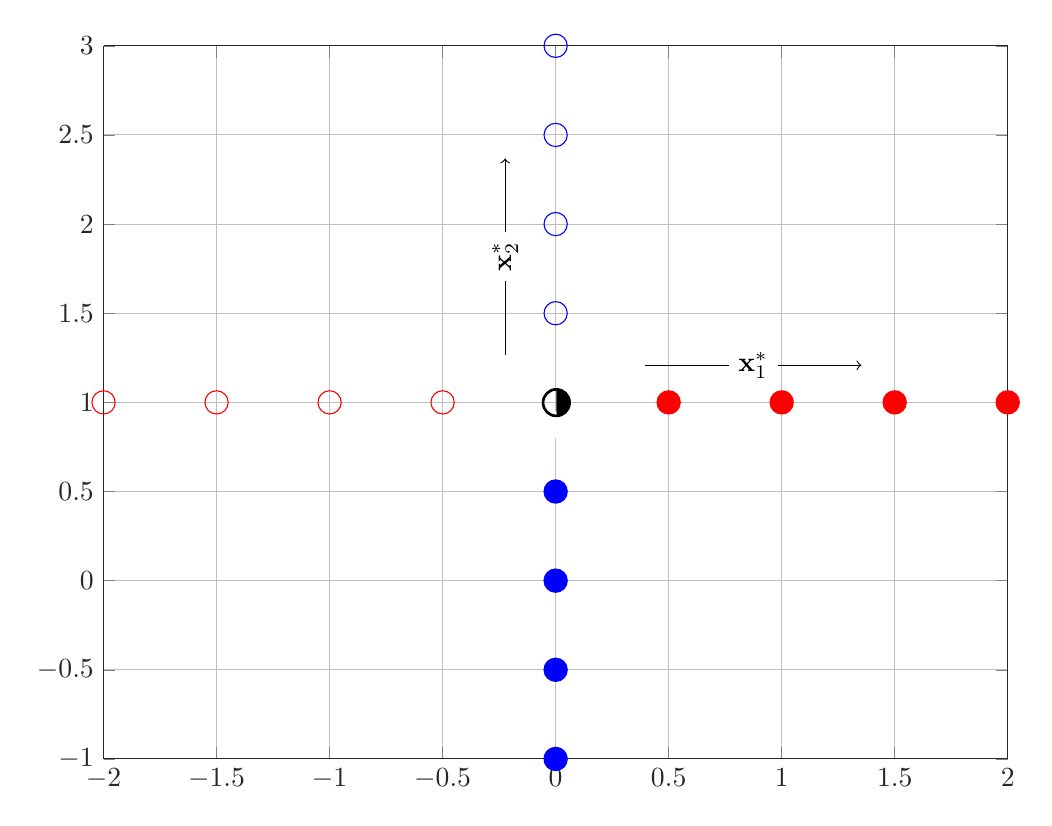
\begin{tikzpicture}

\begin{axis}[%
width=4.52083333333333in,
height=3.565625in,
scale only axis,
separate axis lines,
every outer x axis line/.append style={white!15!black},
every x tick label/.append style={font=\color{white!15!black}},
xmin=-2,
xmax=2,
xmajorgrids,
every outer y axis line/.append style={white!15!black},
every y tick label/.append style={font=\color{white!15!black}},
ymin=-1,
ymax=3,
ymajorgrids
]
\addplot [color=blue,mark size=4.2pt,only marks,mark=*,mark options={solid},forget plot]
  table[row sep=crcr]{0	-1\\
};
\addplot [color=red,only marks,mark size=4.2pt,mark=o,mark options={solid},forget plot]
  table[row sep=crcr]{-2	1\\
};
\addplot [color=blue,mark size=4.2pt,only marks,mark=*,mark options={solid},forget plot]
  table[row sep=crcr]{0	-0.5\\
};
\addplot [color=red,only marks,mark size=4.2pt,mark=o,mark options={solid},forget plot]
  table[row sep=crcr]{-1.5	1\\
};
\addplot [color=blue,mark size=4.2pt,only marks,mark=*,mark options={solid},forget plot]
  table[row sep=crcr]{0	0\\
};
\addplot [color=red,only marks,mark size=4.2pt,mark=o,mark options={solid},forget plot]
  table[row sep=crcr]{-1	1\\
};
\addplot [color=blue,mark size=4.2pt,only marks,mark=*,mark options={solid},forget plot]
  table[row sep=crcr]{0	0.5\\
};
\addplot [color=red,only marks,mark=o,mark size=4.2pt,mark options={solid},forget plot]
  table[row sep=crcr]{-0.5	1\\
};
%\addplot [color=black,mark size=4.2pt,only marks,mark=halfcircle,mark options={solid},forget plot]
%  table[row sep=crcr]{0	1\\
%};
\addplot [color=blue,only marks,mark size=4.2pt,mark=o,mark options={solid},forget plot]
  table[row sep=crcr]{0	1.5\\
};
\addplot [color=red,mark size=4.2pt,only marks,mark=*,mark options={solid},forget plot]
  table[row sep=crcr]{0.5	1\\
};
\addplot [color=blue,only marks,mark size=4.2pt,mark=o,mark options={solid},forget plot]
  table[row sep=crcr]{0	2\\
};
\addplot [color=red,mark size=4.2pt,only marks,mark=*,mark options={solid},forget plot]
  table[row sep=crcr]{1	1\\
};
\addplot [color=blue,only marks,mark size=4.2pt,mark=o,mark options={solid},forget plot]
  table[row sep=crcr]{0	2.5\\
};
\addplot [color=red,mark size=4.2pt,only marks,mark=*,mark options={solid},forget plot]
  table[row sep=crcr]{1.5	1\\
};
\addplot [color=blue,only marks,mark size=4.2pt,mark=o,mark options={solid},forget plot]
  table[row sep=crcr]{0	3\\
};
\addplot [color=red,mark size=4.2pt,only marks,mark=*,mark options={solid},forget plot]
  table[row sep=crcr]{2	1\\
};
\end{axis}

\node [rotate=-90, scale=2.4, text=black] at (5.75, 4.525) {\pgfuseplotmark{halfcircle*}};

\node(n1)       at (6.75,5)    {};
\node(n2)       at (9.75,5)    {};
% this path will place/draw a node call (text)
\path (n1) -- node[sloped] (text) {$\mathbf{x}_1^*$} (n2);
% Now draw arrows. This way it will be like you want.
\draw[->] (n1)--(text)--(n2);
% If you use two draw commands, will get two arrows.
%\draw[->] (n1)--(text);
%\draw[->] (text)--(n2);


\node(n1)       at (5.1,5)    {};
\node(n2)       at (5.1,7.75)    {};
% this path will place/draw a node call (text)
\path (n1) -- node[sloped] (text) {$\mathbf{x}_2^*$} (n2);
% Now draw arrows. This way it will be like you want.
\draw[->] (n1)--(text)--(n2);
% If you use two draw commands, will get two arrows.
%\draw[->] (n1)--(text);
%\draw[->] (text)--(n2);


\end{tikzpicture}%
\end{document}
\caption{Bifurcation diagram for the given system with $f=k=G=1$ and $p \in (-1,3)$. The filled circles indicate stable attracting fixed points. The empty ones symbolize a saddle point. The half filled circle represents a bifurcation.}
\end{figure}


\end{document}
